\documentclass[twoside]{book}

% Packages required by doxygen
\usepackage{calc}
\usepackage{doxygen}
\usepackage{graphicx}
\usepackage[utf8]{inputenc}
\usepackage{makeidx}
\usepackage{multicol}
\usepackage{multirow}
\usepackage{textcomp}
\usepackage[table]{xcolor}

% Font selection
\usepackage[T1]{fontenc}
\usepackage{mathptmx}
\usepackage[scaled=.90]{helvet}
\usepackage{courier}
\usepackage{amssymb}
\usepackage{sectsty}
\renewcommand{\familydefault}{\sfdefault}
\allsectionsfont{%
  \fontseries{bc}\selectfont%
  \color{darkgray}%
}
\renewcommand{\DoxyLabelFont}{%
  \fontseries{bc}\selectfont%
  \color{darkgray}%
}

% Page & text layout
\usepackage{geometry}
\geometry{%
  a4paper,%
  top=2.5cm,%
  bottom=2.5cm,%
  left=2.5cm,%
  right=2.5cm%
}
\tolerance=750
\hfuzz=15pt
\hbadness=750
\setlength{\emergencystretch}{15pt}
\setlength{\parindent}{0cm}
\setlength{\parskip}{0.2cm}
\makeatletter
\renewcommand{\paragraph}{%
  \@startsection{paragraph}{4}{0ex}{-1.0ex}{1.0ex}{%
    \normalfont\normalsize\bfseries\SS@parafont%
  }%
}
\renewcommand{\subparagraph}{%
  \@startsection{subparagraph}{5}{0ex}{-1.0ex}{1.0ex}{%
    \normalfont\normalsize\bfseries\SS@subparafont%
  }%
}
\makeatother

% Headers & footers
\usepackage{fancyhdr}
\pagestyle{fancyplain}
\fancyhead[LE]{\fancyplain{}{\bfseries\thepage}}
\fancyhead[CE]{\fancyplain{}{}}
\fancyhead[RE]{\fancyplain{}{\bfseries\leftmark}}
\fancyhead[LO]{\fancyplain{}{\bfseries\rightmark}}
\fancyhead[CO]{\fancyplain{}{}}
\fancyhead[RO]{\fancyplain{}{\bfseries\thepage}}
\fancyfoot[LE]{\fancyplain{}{}}
\fancyfoot[CE]{\fancyplain{}{}}
\fancyfoot[RE]{\fancyplain{}{\bfseries\scriptsize Generated on Tue Sep 4 2018 21\-:04\-:13 for Reborned\-Gen\-E\-Sy\-S by Doxygen }}
\fancyfoot[LO]{\fancyplain{}{\bfseries\scriptsize Generated on Tue Sep 4 2018 21\-:04\-:13 for Reborned\-Gen\-E\-Sy\-S by Doxygen }}
\fancyfoot[CO]{\fancyplain{}{}}
\fancyfoot[RO]{\fancyplain{}{}}
\renewcommand{\footrulewidth}{0.4pt}
\renewcommand{\chaptermark}[1]{%
  \markboth{#1}{}%
}
\renewcommand{\sectionmark}[1]{%
  \markright{\thesection\ #1}%
}

% Indices & bibliography
\usepackage{natbib}
\usepackage[titles]{tocloft}
\setcounter{tocdepth}{3}
\setcounter{secnumdepth}{5}
\makeindex

% Hyperlinks (required, but should be loaded last)
\usepackage{ifpdf}
\ifpdf
  \usepackage[pdftex,pagebackref=true]{hyperref}
\else
  \usepackage[ps2pdf,pagebackref=true]{hyperref}
\fi
\hypersetup{%
  colorlinks=true,%
  linkcolor=blue,%
  citecolor=blue,%
  unicode%
}

% Custom commands
\newcommand{\clearemptydoublepage}{%
  \newpage{\pagestyle{empty}\cleardoublepage}%
}


%===== C O N T E N T S =====

\begin{document}

% Titlepage & ToC
\hypersetup{pageanchor=false}
\pagenumbering{roman}
\begin{titlepage}
\vspace*{7cm}
\begin{center}%
{\Large Reborned\-Gen\-E\-Sy\-S \\[1ex]\large Reborned 20182 }\\
\vspace*{1cm}
{\large Generated by Doxygen 1.8.6}\\
\vspace*{0.5cm}
{\small Tue Sep 4 2018 21:04:13}\\
\end{center}
\end{titlepage}
\clearemptydoublepage
\tableofcontents
\clearemptydoublepage
\pagenumbering{arabic}
\hypersetup{pageanchor=true}

%--- Begin generated contents ---
\chapter{Gen\-E\-Sy\-S-\/\-Reborn}
\label{md__r_e_a_d_m_e}
\hypertarget{md__r_e_a_d_m_e}{}
\subsubsection*{Generic and Expansible System \hyperlink{class_simulator}{Simulator}}

\subparagraph*{(Work in progress C++ port from the original in Pascal)}

\subparagraph*{Developed by \href{https://github.com/rlcancian}{\tt rlcancian}}
\chapter{Hierarchical Index}
\section{Class Hierarchy}
This inheritance list is sorted roughly, but not completely, alphabetically\-:\begin{DoxyCompactList}
\item \contentsline{section}{Attribute\-Value}{\pageref{class_attribute_value}}{}
\item \contentsline{section}{Collector\-\_\-if}{\pageref{class_collector__if}}{}
\begin{DoxyCompactList}
\item \contentsline{section}{Collector\-Datafile\-\_\-if}{\pageref{class_collector_datafile__if}}{}
\begin{DoxyCompactList}
\item \contentsline{section}{Collector\-Datafile\-My\-Impl1}{\pageref{class_collector_datafile_my_impl1}}{}
\end{DoxyCompactList}
\item \contentsline{section}{Collector\-My\-Impl1}{\pageref{class_collector_my_impl1}}{}
\end{DoxyCompactList}
\item \contentsline{section}{Event}{\pageref{class_event}}{}
\item \contentsline{section}{Fitter\-\_\-if}{\pageref{class_fitter__if}}{}
\begin{DoxyCompactList}
\item \contentsline{section}{Fitter\-My\-Impl1}{\pageref{class_fitter_my_impl1}}{}
\end{DoxyCompactList}
\item \contentsline{section}{Hypothesis\-Tester\-\_\-if}{\pageref{class_hypothesis_tester__if}}{}
\begin{DoxyCompactList}
\item \contentsline{section}{Hypothesis\-Tester\-My\-Impl1}{\pageref{class_hypothesis_tester_my_impl1}}{}
\end{DoxyCompactList}
\item \contentsline{section}{Integrator\-\_\-if}{\pageref{class_integrator__if}}{}
\begin{DoxyCompactList}
\item \contentsline{section}{Integrator\-My\-Impl1}{\pageref{class_integrator_my_impl1}}{}
\end{DoxyCompactList}
\item \contentsline{section}{Linked\-By}{\pageref{class_linked_by}}{}
\begin{DoxyCompactList}
\item \contentsline{section}{Queue}{\pageref{class_queue}}{}
\item \contentsline{section}{Resource}{\pageref{class_resource}}{}
\end{DoxyCompactList}
\item \contentsline{section}{List$<$ T $>$}{\pageref{class_list}}{}
\item \contentsline{section}{List$<$ Event $\ast$ $>$}{\pageref{class_list}}{}
\item \contentsline{section}{List$<$ Model $\ast$ $>$}{\pageref{class_list}}{}
\item \contentsline{section}{List$<$ Model\-Component $\ast$ $>$}{\pageref{class_list}}{}
\item \contentsline{section}{List$<$ Plugin $\ast$ $>$}{\pageref{class_list}}{}
\item \contentsline{section}{List$<$ std\-:\-:string $>$}{\pageref{class_list}}{}
\item \contentsline{section}{List$<$ Waiting $\ast$ $>$}{\pageref{class_list}}{}
\item \contentsline{section}{Model}{\pageref{class_model}}{}
\item \contentsline{section}{Model\-Checker\-\_\-if}{\pageref{class_model_checker__if}}{}
\begin{DoxyCompactList}
\item \contentsline{section}{Model\-Checker\-My\-Impl1}{\pageref{class_model_checker_my_impl1}}{}
\end{DoxyCompactList}
\item \contentsline{section}{Model\-Infrastructure}{\pageref{class_model_infrastructure}}{}
\begin{DoxyCompactList}
\item \contentsline{section}{Entity}{\pageref{class_entity}}{}
\item \contentsline{section}{Entity\-Type}{\pageref{class_entity_type}}{}
\item \contentsline{section}{Model\-Component}{\pageref{class_model_component}}{}
\begin{DoxyCompactList}
\item \contentsline{section}{Assign}{\pageref{class_assign}}{}
\item \contentsline{section}{Delay}{\pageref{class_delay}}{}
\item \contentsline{section}{Release}{\pageref{class_release}}{}
\item \contentsline{section}{Seize}{\pageref{class_seize}}{}
\item \contentsline{section}{Sink\-Model\-Component}{\pageref{class_sink_model_component}}{}
\begin{DoxyCompactList}
\item \contentsline{section}{Dispose}{\pageref{class_dispose}}{}
\end{DoxyCompactList}
\item \contentsline{section}{Source\-Model\-Component}{\pageref{class_source_model_component}}{}
\begin{DoxyCompactList}
\item \contentsline{section}{Create}{\pageref{class_create}}{}
\end{DoxyCompactList}
\end{DoxyCompactList}
\item \contentsline{section}{Queue}{\pageref{class_queue}}{}
\item \contentsline{section}{Resource}{\pageref{class_resource}}{}
\item \contentsline{section}{Statistics\-Collector}{\pageref{class_statistics_collector}}{}
\item \contentsline{section}{Variable}{\pageref{class_variable}}{}
\end{DoxyCompactList}
\item \contentsline{section}{Model\-Persistence\-\_\-if}{\pageref{class_model_persistence__if}}{}
\begin{DoxyCompactList}
\item \contentsline{section}{Model\-Persistence\-My\-Impl1}{\pageref{class_model_persistence_my_impl1}}{}
\end{DoxyCompactList}
\item \contentsline{section}{Parser\-\_\-if}{\pageref{class_parser__if}}{}
\begin{DoxyCompactList}
\item \contentsline{section}{Parser\-My\-Impl1}{\pageref{class_parser_my_impl1}}{}
\end{DoxyCompactList}
\item \contentsline{section}{Plugin}{\pageref{class_plugin}}{}
\item \contentsline{section}{Prob\-Distrib}{\pageref{class_prob_distrib}}{}
\item \contentsline{section}{Sampler\-\_\-if\-:\-:R\-N\-G\-\_\-\-Parameters}{\pageref{class_sampler__if_1_1_r_n_g___parameters}}{}
\begin{DoxyCompactList}
\item \contentsline{section}{Sampler\-My\-Impl1\-:\-:My\-R\-N\-G\-\_\-\-Parameters}{\pageref{class_sampler_my_impl1_1_1_my_r_n_g___parameters}}{}
\end{DoxyCompactList}
\item \contentsline{section}{Sampler\-\_\-if}{\pageref{class_sampler__if}}{}
\begin{DoxyCompactList}
\item \contentsline{section}{Sampler\-My\-Impl1}{\pageref{class_sampler_my_impl1}}{}
\end{DoxyCompactList}
\item \contentsline{section}{Simulator}{\pageref{class_simulator}}{}
\item \contentsline{section}{Statistics\-\_\-if}{\pageref{class_statistics__if}}{}
\begin{DoxyCompactList}
\item \contentsline{section}{Statistics\-My\-Impl1}{\pageref{class_statistics_my_impl1}}{}
\begin{DoxyCompactList}
\item \contentsline{section}{Statistics\-Collector}{\pageref{class_statistics_collector}}{}
\end{DoxyCompactList}
\end{DoxyCompactList}
\item \contentsline{section}{Trace\-Event}{\pageref{class_trace_event}}{}
\begin{DoxyCompactList}
\item \contentsline{section}{Trace\-Error\-Event}{\pageref{class_trace_error_event}}{}
\item \contentsline{section}{Trace\-Simulation\-Event}{\pageref{class_trace_simulation_event}}{}
\end{DoxyCompactList}
\item \contentsline{section}{Traits$<$ T $>$}{\pageref{struct_traits}}{}
\item \contentsline{section}{Traits$<$ Collector\-\_\-if $>$}{\pageref{struct_traits_3_01_collector__if_01_4}}{}
\item \contentsline{section}{Traits$<$ Fitter\-\_\-if $>$}{\pageref{struct_traits_3_01_fitter__if_01_4}}{}
\item \contentsline{section}{Traits$<$ Hypothesis\-Tester\-\_\-if $>$}{\pageref{struct_traits_3_01_hypothesis_tester__if_01_4}}{}
\item \contentsline{section}{Traits$<$ Integrator\-\_\-if $>$}{\pageref{struct_traits_3_01_integrator__if_01_4}}{}
\item \contentsline{section}{Traits$<$ Model $>$}{\pageref{struct_traits_3_01_model_01_4}}{}
\item \contentsline{section}{Traits$<$ Model\-Checker\-\_\-if $>$}{\pageref{struct_traits_3_01_model_checker__if_01_4}}{}
\item \contentsline{section}{Traits$<$ Model\-Component $>$}{\pageref{struct_traits_3_01_model_component_01_4}}{}
\item \contentsline{section}{Traits$<$ Model\-Persistence\-\_\-if $>$}{\pageref{struct_traits_3_01_model_persistence__if_01_4}}{}
\item \contentsline{section}{Traits$<$ Parser\-\_\-if $>$}{\pageref{struct_traits_3_01_parser__if_01_4}}{}
\item \contentsline{section}{Traits$<$ Sampler\-\_\-if $>$}{\pageref{struct_traits_3_01_sampler__if_01_4}}{}
\item \contentsline{section}{Traits$<$ Statistics\-\_\-if $>$}{\pageref{struct_traits_3_01_statistics__if_01_4}}{}
\item \contentsline{section}{Util}{\pageref{class_util}}{}
\item \contentsline{section}{Waiting}{\pageref{class_waiting}}{}
\begin{DoxyCompactList}
\item \contentsline{section}{Waiting\-Resource}{\pageref{class_waiting_resource}}{}
\end{DoxyCompactList}
\end{DoxyCompactList}

\chapter{Class Index}
\section{Class List}
Here are the classes, structs, unions and interfaces with brief descriptions\-:\begin{DoxyCompactList}
\item\contentsline{section}{\hyperlink{class_assign}{Assign} }{\pageref{class_assign}}{}
\item\contentsline{section}{\hyperlink{class_attribute_value}{Attribute\-Value} }{\pageref{class_attribute_value}}{}
\item\contentsline{section}{\hyperlink{class_collector__if}{Collector\-\_\-if} }{\pageref{class_collector__if}}{}
\item\contentsline{section}{\hyperlink{class_collector_datafile__if}{Collector\-Datafile\-\_\-if} }{\pageref{class_collector_datafile__if}}{}
\item\contentsline{section}{\hyperlink{class_collector_datafile_my_impl1}{Collector\-Datafile\-My\-Impl1} }{\pageref{class_collector_datafile_my_impl1}}{}
\item\contentsline{section}{\hyperlink{class_collector_my_impl1}{Collector\-My\-Impl1} }{\pageref{class_collector_my_impl1}}{}
\item\contentsline{section}{\hyperlink{class_create}{Create} }{\pageref{class_create}}{}
\item\contentsline{section}{\hyperlink{class_delay}{Delay} }{\pageref{class_delay}}{}
\item\contentsline{section}{\hyperlink{class_dispose}{Dispose} }{\pageref{class_dispose}}{}
\item\contentsline{section}{\hyperlink{class_entity}{Entity} }{\pageref{class_entity}}{}
\item\contentsline{section}{\hyperlink{class_entity_type}{Entity\-Type} }{\pageref{class_entity_type}}{}
\item\contentsline{section}{\hyperlink{class_event}{Event} }{\pageref{class_event}}{}
\item\contentsline{section}{\hyperlink{class_fitter__if}{Fitter\-\_\-if} }{\pageref{class_fitter__if}}{}
\item\contentsline{section}{\hyperlink{class_fitter_my_impl1}{Fitter\-My\-Impl1} }{\pageref{class_fitter_my_impl1}}{}
\item\contentsline{section}{\hyperlink{class_hypothesis_tester__if}{Hypothesis\-Tester\-\_\-if} }{\pageref{class_hypothesis_tester__if}}{}
\item\contentsline{section}{\hyperlink{class_hypothesis_tester_my_impl1}{Hypothesis\-Tester\-My\-Impl1} }{\pageref{class_hypothesis_tester_my_impl1}}{}
\item\contentsline{section}{\hyperlink{class_integrator__if}{Integrator\-\_\-if} }{\pageref{class_integrator__if}}{}
\item\contentsline{section}{\hyperlink{class_integrator_my_impl1}{Integrator\-My\-Impl1} }{\pageref{class_integrator_my_impl1}}{}
\item\contentsline{section}{\hyperlink{class_linked_by}{Linked\-By} }{\pageref{class_linked_by}}{}
\item\contentsline{section}{\hyperlink{class_list}{List$<$ T $>$} }{\pageref{class_list}}{}
\item\contentsline{section}{\hyperlink{class_model}{Model} }{\pageref{class_model}}{}
\item\contentsline{section}{\hyperlink{class_model_checker__if}{Model\-Checker\-\_\-if} }{\pageref{class_model_checker__if}}{}
\item\contentsline{section}{\hyperlink{class_model_checker_my_impl1}{Model\-Checker\-My\-Impl1} }{\pageref{class_model_checker_my_impl1}}{}
\item\contentsline{section}{\hyperlink{class_model_component}{Model\-Component} }{\pageref{class_model_component}}{}
\item\contentsline{section}{\hyperlink{class_model_infrastructure}{Model\-Infrastructure} }{\pageref{class_model_infrastructure}}{}
\item\contentsline{section}{\hyperlink{class_model_persistence__if}{Model\-Persistence\-\_\-if} }{\pageref{class_model_persistence__if}}{}
\item\contentsline{section}{\hyperlink{class_model_persistence_my_impl1}{Model\-Persistence\-My\-Impl1} }{\pageref{class_model_persistence_my_impl1}}{}
\item\contentsline{section}{\hyperlink{class_sampler_my_impl1_1_1_my_r_n_g___parameters}{Sampler\-My\-Impl1\-::\-My\-R\-N\-G\-\_\-\-Parameters} }{\pageref{class_sampler_my_impl1_1_1_my_r_n_g___parameters}}{}
\item\contentsline{section}{\hyperlink{class_parser__if}{Parser\-\_\-if} }{\pageref{class_parser__if}}{}
\item\contentsline{section}{\hyperlink{class_parser_my_impl1}{Parser\-My\-Impl1} }{\pageref{class_parser_my_impl1}}{}
\item\contentsline{section}{\hyperlink{class_plugin}{Plugin} }{\pageref{class_plugin}}{}
\item\contentsline{section}{\hyperlink{class_prob_distrib}{Prob\-Distrib} }{\pageref{class_prob_distrib}}{}
\item\contentsline{section}{\hyperlink{class_queue}{Queue} }{\pageref{class_queue}}{}
\item\contentsline{section}{\hyperlink{class_release}{Release} }{\pageref{class_release}}{}
\item\contentsline{section}{\hyperlink{class_resource}{Resource} }{\pageref{class_resource}}{}
\item\contentsline{section}{\hyperlink{class_sampler__if_1_1_r_n_g___parameters}{Sampler\-\_\-if\-::\-R\-N\-G\-\_\-\-Parameters} }{\pageref{class_sampler__if_1_1_r_n_g___parameters}}{}
\item\contentsline{section}{\hyperlink{class_sampler__if}{Sampler\-\_\-if} }{\pageref{class_sampler__if}}{}
\item\contentsline{section}{\hyperlink{class_sampler_my_impl1}{Sampler\-My\-Impl1} }{\pageref{class_sampler_my_impl1}}{}
\item\contentsline{section}{\hyperlink{class_seize}{Seize} }{\pageref{class_seize}}{}
\item\contentsline{section}{\hyperlink{class_simulator}{Simulator} }{\pageref{class_simulator}}{}
\item\contentsline{section}{\hyperlink{class_sink_model_component}{Sink\-Model\-Component} }{\pageref{class_sink_model_component}}{}
\item\contentsline{section}{\hyperlink{class_source_model_component}{Source\-Model\-Component} }{\pageref{class_source_model_component}}{}
\item\contentsline{section}{\hyperlink{class_statistics__if}{Statistics\-\_\-if} }{\pageref{class_statistics__if}}{}
\item\contentsline{section}{\hyperlink{class_statistics_collector}{Statistics\-Collector} }{\pageref{class_statistics_collector}}{}
\item\contentsline{section}{\hyperlink{class_statistics_my_impl1}{Statistics\-My\-Impl1} }{\pageref{class_statistics_my_impl1}}{}
\item\contentsline{section}{\hyperlink{class_trace_error_event}{Trace\-Error\-Event} }{\pageref{class_trace_error_event}}{}
\item\contentsline{section}{\hyperlink{class_trace_event}{Trace\-Event} }{\pageref{class_trace_event}}{}
\item\contentsline{section}{\hyperlink{class_trace_simulation_event}{Trace\-Simulation\-Event} }{\pageref{class_trace_simulation_event}}{}
\item\contentsline{section}{\hyperlink{struct_traits}{Traits$<$ T $>$} }{\pageref{struct_traits}}{}
\item\contentsline{section}{\hyperlink{struct_traits_3_01_collector__if_01_4}{Traits$<$ Collector\-\_\-if $>$} }{\pageref{struct_traits_3_01_collector__if_01_4}}{}
\item\contentsline{section}{\hyperlink{struct_traits_3_01_fitter__if_01_4}{Traits$<$ Fitter\-\_\-if $>$} }{\pageref{struct_traits_3_01_fitter__if_01_4}}{}
\item\contentsline{section}{\hyperlink{struct_traits_3_01_hypothesis_tester__if_01_4}{Traits$<$ Hypothesis\-Tester\-\_\-if $>$} }{\pageref{struct_traits_3_01_hypothesis_tester__if_01_4}}{}
\item\contentsline{section}{\hyperlink{struct_traits_3_01_integrator__if_01_4}{Traits$<$ Integrator\-\_\-if $>$} }{\pageref{struct_traits_3_01_integrator__if_01_4}}{}
\item\contentsline{section}{\hyperlink{struct_traits_3_01_model_01_4}{Traits$<$ Model $>$} }{\pageref{struct_traits_3_01_model_01_4}}{}
\item\contentsline{section}{\hyperlink{struct_traits_3_01_model_checker__if_01_4}{Traits$<$ Model\-Checker\-\_\-if $>$} }{\pageref{struct_traits_3_01_model_checker__if_01_4}}{}
\item\contentsline{section}{\hyperlink{struct_traits_3_01_model_component_01_4}{Traits$<$ Model\-Component $>$} }{\pageref{struct_traits_3_01_model_component_01_4}}{}
\item\contentsline{section}{\hyperlink{struct_traits_3_01_model_persistence__if_01_4}{Traits$<$ Model\-Persistence\-\_\-if $>$} }{\pageref{struct_traits_3_01_model_persistence__if_01_4}}{}
\item\contentsline{section}{\hyperlink{struct_traits_3_01_parser__if_01_4}{Traits$<$ Parser\-\_\-if $>$} }{\pageref{struct_traits_3_01_parser__if_01_4}}{}
\item\contentsline{section}{\hyperlink{struct_traits_3_01_sampler__if_01_4}{Traits$<$ Sampler\-\_\-if $>$} }{\pageref{struct_traits_3_01_sampler__if_01_4}}{}
\item\contentsline{section}{\hyperlink{struct_traits_3_01_statistics__if_01_4}{Traits$<$ Statistics\-\_\-if $>$} }{\pageref{struct_traits_3_01_statistics__if_01_4}}{}
\item\contentsline{section}{\hyperlink{class_util}{Util} }{\pageref{class_util}}{}
\item\contentsline{section}{\hyperlink{class_variable}{Variable} }{\pageref{class_variable}}{}
\item\contentsline{section}{\hyperlink{class_waiting}{Waiting} }{\pageref{class_waiting}}{}
\item\contentsline{section}{\hyperlink{class_waiting_resource}{Waiting\-Resource} }{\pageref{class_waiting_resource}}{}
\end{DoxyCompactList}

\chapter{File Index}
\section{File List}
Here is a list of all files with brief descriptions\-:\begin{DoxyCompactList}
\item\contentsline{section}{\hyperlink{_8dep_8inc}{.\-dep.\-inc} }{\pageref{_8dep_8inc}}{}
\item\contentsline{section}{\hyperlink{_assign_8cpp}{Assign.\-cpp} }{\pageref{_assign_8cpp}}{}
\item\contentsline{section}{\hyperlink{_assign_8h}{Assign.\-h} }{\pageref{_assign_8h}}{}
\item\contentsline{section}{\hyperlink{_attribute_value_8cpp}{Attribute\-Value.\-cpp} }{\pageref{_attribute_value_8cpp}}{}
\item\contentsline{section}{\hyperlink{_attribute_value_8h}{Attribute\-Value.\-h} }{\pageref{_attribute_value_8h}}{}
\item\contentsline{section}{\hyperlink{_collector__if_8h}{Collector\-\_\-if.\-h} }{\pageref{_collector__if_8h}}{}
\item\contentsline{section}{\hyperlink{_collector_datafile__if_8h}{Collector\-Datafile\-\_\-if.\-h} }{\pageref{_collector_datafile__if_8h}}{}
\item\contentsline{section}{\hyperlink{_collector_datafile_my_impl1_8cpp}{Collector\-Datafile\-My\-Impl1.\-cpp} }{\pageref{_collector_datafile_my_impl1_8cpp}}{}
\item\contentsline{section}{\hyperlink{_collector_datafile_my_impl1_8h}{Collector\-Datafile\-My\-Impl1.\-h} }{\pageref{_collector_datafile_my_impl1_8h}}{}
\item\contentsline{section}{\hyperlink{_collector_my_impl1_8cpp}{Collector\-My\-Impl1.\-cpp} }{\pageref{_collector_my_impl1_8cpp}}{}
\item\contentsline{section}{\hyperlink{_collector_my_impl1_8h}{Collector\-My\-Impl1.\-h} }{\pageref{_collector_my_impl1_8h}}{}
\item\contentsline{section}{\hyperlink{_create_8cpp}{Create.\-cpp} }{\pageref{_create_8cpp}}{}
\item\contentsline{section}{\hyperlink{_create_8h}{Create.\-h} }{\pageref{_create_8h}}{}
\item\contentsline{section}{\hyperlink{_delay_8cpp}{Delay.\-cpp} }{\pageref{_delay_8cpp}}{}
\item\contentsline{section}{\hyperlink{_delay_8h}{Delay.\-h} }{\pageref{_delay_8h}}{}
\item\contentsline{section}{\hyperlink{_dispose_8cpp}{Dispose.\-cpp} }{\pageref{_dispose_8cpp}}{}
\item\contentsline{section}{\hyperlink{_dispose_8h}{Dispose.\-h} }{\pageref{_dispose_8h}}{}
\item\contentsline{section}{\hyperlink{_entity_8cpp}{Entity.\-cpp} }{\pageref{_entity_8cpp}}{}
\item\contentsline{section}{\hyperlink{_entity_8h}{Entity.\-h} }{\pageref{_entity_8h}}{}
\item\contentsline{section}{\hyperlink{_entity_type_8cpp}{Entity\-Type.\-cpp} }{\pageref{_entity_type_8cpp}}{}
\item\contentsline{section}{\hyperlink{_entity_type_8h}{Entity\-Type.\-h} }{\pageref{_entity_type_8h}}{}
\item\contentsline{section}{\hyperlink{_event_8cpp}{Event.\-cpp} }{\pageref{_event_8cpp}}{}
\item\contentsline{section}{\hyperlink{_event_8h}{Event.\-h} }{\pageref{_event_8h}}{}
\item\contentsline{section}{\hyperlink{_fitter__if_8h}{Fitter\-\_\-if.\-h} }{\pageref{_fitter__if_8h}}{}
\item\contentsline{section}{\hyperlink{_fitter_my_impl1_8cpp}{Fitter\-My\-Impl1.\-cpp} }{\pageref{_fitter_my_impl1_8cpp}}{}
\item\contentsline{section}{\hyperlink{_fitter_my_impl1_8h}{Fitter\-My\-Impl1.\-h} }{\pageref{_fitter_my_impl1_8h}}{}
\item\contentsline{section}{\hyperlink{_hypothesis_tester__if_8h}{Hypothesis\-Tester\-\_\-if.\-h} }{\pageref{_hypothesis_tester__if_8h}}{}
\item\contentsline{section}{\hyperlink{_hypothesis_tester_my_impl1_8cpp}{Hypothesis\-Tester\-My\-Impl1.\-cpp} }{\pageref{_hypothesis_tester_my_impl1_8cpp}}{}
\item\contentsline{section}{\hyperlink{_hypothesis_tester_my_impl1_8h}{Hypothesis\-Tester\-My\-Impl1.\-h} }{\pageref{_hypothesis_tester_my_impl1_8h}}{}
\item\contentsline{section}{\hyperlink{_integrator__if_8h}{Integrator\-\_\-if.\-h} }{\pageref{_integrator__if_8h}}{}
\item\contentsline{section}{\hyperlink{_integrator_my_impl1_8cpp}{Integrator\-My\-Impl1.\-cpp} }{\pageref{_integrator_my_impl1_8cpp}}{}
\item\contentsline{section}{\hyperlink{_integrator_my_impl1_8h}{Integrator\-My\-Impl1.\-h} }{\pageref{_integrator_my_impl1_8h}}{}
\item\contentsline{section}{\hyperlink{_linked_by_8cpp}{Linked\-By.\-cpp} }{\pageref{_linked_by_8cpp}}{}
\item\contentsline{section}{\hyperlink{_linked_by_8h}{Linked\-By.\-h} }{\pageref{_linked_by_8h}}{}
\item\contentsline{section}{\hyperlink{_list_8h}{List.\-h} }{\pageref{_list_8h}}{}
\item\contentsline{section}{\hyperlink{_listener_8cpp}{Listener.\-cpp} }{\pageref{_listener_8cpp}}{}
\item\contentsline{section}{\hyperlink{_listener_8h}{Listener.\-h} }{\pageref{_listener_8h}}{}
\item\contentsline{section}{\hyperlink{main_8cpp}{main.\-cpp} }{\pageref{main_8cpp}}{}
\item\contentsline{section}{\hyperlink{_model_8cpp}{Model.\-cpp} }{\pageref{_model_8cpp}}{}
\item\contentsline{section}{\hyperlink{_model_8h}{Model.\-h} }{\pageref{_model_8h}}{}
\item\contentsline{section}{\hyperlink{_model_checker__if_8h}{Model\-Checker\-\_\-if.\-h} }{\pageref{_model_checker__if_8h}}{}
\item\contentsline{section}{\hyperlink{_model_checker_my_impl1_8cpp}{Model\-Checker\-My\-Impl1.\-cpp} }{\pageref{_model_checker_my_impl1_8cpp}}{}
\item\contentsline{section}{\hyperlink{_model_checker_my_impl1_8h}{Model\-Checker\-My\-Impl1.\-h} }{\pageref{_model_checker_my_impl1_8h}}{}
\item\contentsline{section}{\hyperlink{_model_component_8cpp}{Model\-Component.\-cpp} }{\pageref{_model_component_8cpp}}{}
\item\contentsline{section}{\hyperlink{_model_component_8h}{Model\-Component.\-h} }{\pageref{_model_component_8h}}{}
\item\contentsline{section}{\hyperlink{_model_infrastructure_8cpp}{Model\-Infrastructure.\-cpp} }{\pageref{_model_infrastructure_8cpp}}{}
\item\contentsline{section}{\hyperlink{_model_infrastructure_8h}{Model\-Infrastructure.\-h} }{\pageref{_model_infrastructure_8h}}{}
\item\contentsline{section}{\hyperlink{_model_persistence__if_8h}{Model\-Persistence\-\_\-if.\-h} }{\pageref{_model_persistence__if_8h}}{}
\item\contentsline{section}{\hyperlink{_model_persistence_my_impl1_8cpp}{Model\-Persistence\-My\-Impl1.\-cpp} }{\pageref{_model_persistence_my_impl1_8cpp}}{}
\item\contentsline{section}{\hyperlink{_model_persistence_my_impl1_8h}{Model\-Persistence\-My\-Impl1.\-h} }{\pageref{_model_persistence_my_impl1_8h}}{}
\item\contentsline{section}{\hyperlink{_parser__if_8h}{Parser\-\_\-if.\-h} }{\pageref{_parser__if_8h}}{}
\item\contentsline{section}{\hyperlink{_parser_my_impl1_8cpp}{Parser\-My\-Impl1.\-cpp} }{\pageref{_parser_my_impl1_8cpp}}{}
\item\contentsline{section}{\hyperlink{_parser_my_impl1_8h}{Parser\-My\-Impl1.\-h} }{\pageref{_parser_my_impl1_8h}}{}
\item\contentsline{section}{\hyperlink{_plugin_8cpp}{Plugin.\-cpp} }{\pageref{_plugin_8cpp}}{}
\item\contentsline{section}{\hyperlink{_plugin_8h}{Plugin.\-h} }{\pageref{_plugin_8h}}{}
\item\contentsline{section}{\hyperlink{_prob_distrib_8cpp}{Prob\-Distrib.\-cpp} }{\pageref{_prob_distrib_8cpp}}{}
\item\contentsline{section}{\hyperlink{_prob_distrib_8h}{Prob\-Distrib.\-h} }{\pageref{_prob_distrib_8h}}{}
\item\contentsline{section}{\hyperlink{_queue_8cpp}{Queue.\-cpp} }{\pageref{_queue_8cpp}}{}
\item\contentsline{section}{\hyperlink{_queue_8h}{Queue.\-h} }{\pageref{_queue_8h}}{}
\item\contentsline{section}{\hyperlink{_release_8cpp}{Release.\-cpp} }{\pageref{_release_8cpp}}{}
\item\contentsline{section}{\hyperlink{_release_8h}{Release.\-h} }{\pageref{_release_8h}}{}
\item\contentsline{section}{\hyperlink{_resource_8cpp}{Resource.\-cpp} }{\pageref{_resource_8cpp}}{}
\item\contentsline{section}{\hyperlink{_resource_8h}{Resource.\-h} }{\pageref{_resource_8h}}{}
\item\contentsline{section}{\hyperlink{_sampler__if_8h}{Sampler\-\_\-if.\-h} }{\pageref{_sampler__if_8h}}{}
\item\contentsline{section}{\hyperlink{_sampler_my_impl1_8cpp}{Sampler\-My\-Impl1.\-cpp} }{\pageref{_sampler_my_impl1_8cpp}}{}
\item\contentsline{section}{\hyperlink{_sampler_my_impl1_8h}{Sampler\-My\-Impl1.\-h} }{\pageref{_sampler_my_impl1_8h}}{}
\item\contentsline{section}{\hyperlink{_seize_8cpp}{Seize.\-cpp} }{\pageref{_seize_8cpp}}{}
\item\contentsline{section}{\hyperlink{_seize_8h}{Seize.\-h} }{\pageref{_seize_8h}}{}
\item\contentsline{section}{\hyperlink{_simulator_8cpp}{Simulator.\-cpp} }{\pageref{_simulator_8cpp}}{}
\item\contentsline{section}{\hyperlink{_simulator_8h}{Simulator.\-h} }{\pageref{_simulator_8h}}{}
\item\contentsline{section}{\hyperlink{_sink_model_component_8cpp}{Sink\-Model\-Component.\-cpp} }{\pageref{_sink_model_component_8cpp}}{}
\item\contentsline{section}{\hyperlink{_sink_model_component_8h}{Sink\-Model\-Component.\-h} }{\pageref{_sink_model_component_8h}}{}
\item\contentsline{section}{\hyperlink{_source_model_component_8cpp}{Source\-Model\-Component.\-cpp} }{\pageref{_source_model_component_8cpp}}{}
\item\contentsline{section}{\hyperlink{_source_model_component_8h}{Source\-Model\-Component.\-h} }{\pageref{_source_model_component_8h}}{}
\item\contentsline{section}{\hyperlink{_statistics__if_8h}{Statistics\-\_\-if.\-h} }{\pageref{_statistics__if_8h}}{}
\item\contentsline{section}{\hyperlink{_statistics_collector_8cpp}{Statistics\-Collector.\-cpp} }{\pageref{_statistics_collector_8cpp}}{}
\item\contentsline{section}{\hyperlink{_statistics_collector_8h}{Statistics\-Collector.\-h} }{\pageref{_statistics_collector_8h}}{}
\item\contentsline{section}{\hyperlink{_statistics_my_impl1_8cpp}{Statistics\-My\-Impl1.\-cpp} }{\pageref{_statistics_my_impl1_8cpp}}{}
\item\contentsline{section}{\hyperlink{_statistics_my_impl1_8h}{Statistics\-My\-Impl1.\-h} }{\pageref{_statistics_my_impl1_8h}}{}
\item\contentsline{section}{\hyperlink{_traits_8h}{Traits.\-h} }{\pageref{_traits_8h}}{}
\item\contentsline{section}{\hyperlink{_util_8cpp}{Util.\-cpp} }{\pageref{_util_8cpp}}{}
\item\contentsline{section}{\hyperlink{_util_8h}{Util.\-h} }{\pageref{_util_8h}}{}
\item\contentsline{section}{\hyperlink{_variable_8cpp}{Variable.\-cpp} }{\pageref{_variable_8cpp}}{}
\item\contentsline{section}{\hyperlink{_variable_8h}{Variable.\-h} }{\pageref{_variable_8h}}{}
\item\contentsline{section}{\hyperlink{_waiting_8cpp}{Waiting.\-cpp} }{\pageref{_waiting_8cpp}}{}
\item\contentsline{section}{\hyperlink{_waiting_8h}{Waiting.\-h} }{\pageref{_waiting_8h}}{}
\item\contentsline{section}{\hyperlink{_waiting_resource_8cpp}{Waiting\-Resource.\-cpp} }{\pageref{_waiting_resource_8cpp}}{}
\item\contentsline{section}{\hyperlink{_waiting_resource_8h}{Waiting\-Resource.\-h} }{\pageref{_waiting_resource_8h}}{}
\end{DoxyCompactList}

\chapter{Class Documentation}
\hypertarget{class_assign}{\section{Assign Class Reference}
\label{class_assign}\index{Assign@{Assign}}
}


{\ttfamily \#include $<$Assign.\-h$>$}



Inheritance diagram for Assign\-:\nopagebreak
\begin{figure}[H]
\begin{center}
\leavevmode
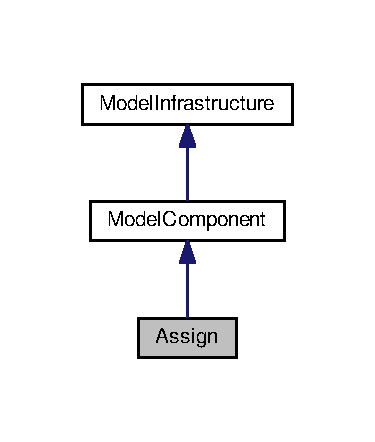
\includegraphics[width=180pt]{class_assign__inherit__graph}
\end{center}
\end{figure}


Collaboration diagram for Assign\-:\nopagebreak
\begin{figure}[H]
\begin{center}
\leavevmode
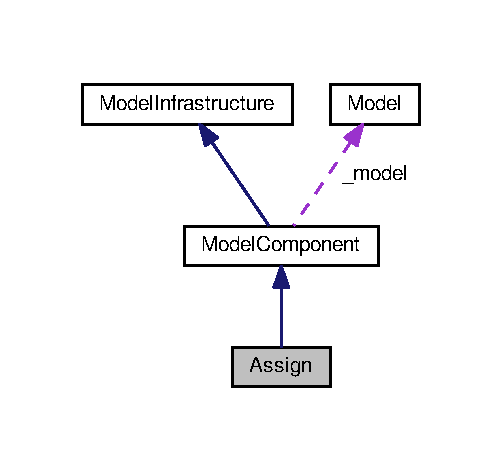
\includegraphics[width=241pt]{class_assign__coll__graph}
\end{center}
\end{figure}
\subsection*{Public Member Functions}
\begin{DoxyCompactItemize}
\item 
\hyperlink{class_assign_afaa746a0ce157d4606823ad508dc6281}{Assign} (\hyperlink{class_model}{Model} $\ast$model)
\item 
\hyperlink{class_assign_ae4945adcf1b5dcdd3f57faa9dd85a2b0}{Assign} (const \hyperlink{class_assign}{Assign} \&orig)
\item 
virtual \hyperlink{class_assign_aa005626af06022d9101c5e38e794dc47}{$\sim$\-Assign} ()
\item 
virtual std\-::string \hyperlink{class_assign_af5022b92204adcd9ee3e444b7e316d07}{show} ()
\end{DoxyCompactItemize}
\subsection*{Protected Member Functions}
\begin{DoxyCompactItemize}
\item 
virtual void \hyperlink{class_assign_a5fabf69268b2e65d8b01ce247be87a40}{\-\_\-execute} (\hyperlink{class_entity}{Entity} $\ast$entity)
\item 
virtual void \hyperlink{class_assign_a47728ac75ef40025f00cca46e04dd012}{\-\_\-read\-Component} (std\-::list$<$ std\-::string $>$ words)
\item 
virtual std\-::list$<$ std\-::string $>$ $\ast$ \hyperlink{class_assign_a6231f1e819d6baab3c9af142fd5b566a}{\-\_\-write\-Component} ()
\item 
virtual bool \hyperlink{class_assign_a5f3a7d8a7214574fea926cae1b1acb94}{\-\_\-verify\-Symbols} (std\-::string $\ast$error\-Message)
\end{DoxyCompactItemize}
\subsection*{Additional Inherited Members}


\subsection{Constructor \& Destructor Documentation}
\hypertarget{class_assign_afaa746a0ce157d4606823ad508dc6281}{\index{Assign@{Assign}!Assign@{Assign}}
\index{Assign@{Assign}!Assign@{Assign}}
\subsubsection[{Assign}]{\setlength{\rightskip}{0pt plus 5cm}Assign\-::\-Assign (
\begin{DoxyParamCaption}
\item[{{\bf Model} $\ast$}]{model}
\end{DoxyParamCaption}
)}}\label{class_assign_afaa746a0ce157d4606823ad508dc6281}
\hypertarget{class_assign_ae4945adcf1b5dcdd3f57faa9dd85a2b0}{\index{Assign@{Assign}!Assign@{Assign}}
\index{Assign@{Assign}!Assign@{Assign}}
\subsubsection[{Assign}]{\setlength{\rightskip}{0pt plus 5cm}Assign\-::\-Assign (
\begin{DoxyParamCaption}
\item[{const {\bf Assign} \&}]{orig}
\end{DoxyParamCaption}
)}}\label{class_assign_ae4945adcf1b5dcdd3f57faa9dd85a2b0}
\hypertarget{class_assign_aa005626af06022d9101c5e38e794dc47}{\index{Assign@{Assign}!$\sim$\-Assign@{$\sim$\-Assign}}
\index{$\sim$\-Assign@{$\sim$\-Assign}!Assign@{Assign}}
\subsubsection[{$\sim$\-Assign}]{\setlength{\rightskip}{0pt plus 5cm}Assign\-::$\sim$\-Assign (
\begin{DoxyParamCaption}
{}
\end{DoxyParamCaption}
)\hspace{0.3cm}{\ttfamily [virtual]}}}\label{class_assign_aa005626af06022d9101c5e38e794dc47}


\subsection{Member Function Documentation}
\hypertarget{class_assign_a5fabf69268b2e65d8b01ce247be87a40}{\index{Assign@{Assign}!\-\_\-execute@{\-\_\-execute}}
\index{\-\_\-execute@{\-\_\-execute}!Assign@{Assign}}
\subsubsection[{\-\_\-execute}]{\setlength{\rightskip}{0pt plus 5cm}void Assign\-::\-\_\-execute (
\begin{DoxyParamCaption}
\item[{{\bf Entity} $\ast$}]{entity}
\end{DoxyParamCaption}
)\hspace{0.3cm}{\ttfamily [protected]}, {\ttfamily [virtual]}}}\label{class_assign_a5fabf69268b2e65d8b01ce247be87a40}


Implements \hyperlink{class_model_component_ae3fcf8bbdd8368c882438424aa73f714}{Model\-Component}.



Here is the call graph for this function\-:\nopagebreak
\begin{figure}[H]
\begin{center}
\leavevmode
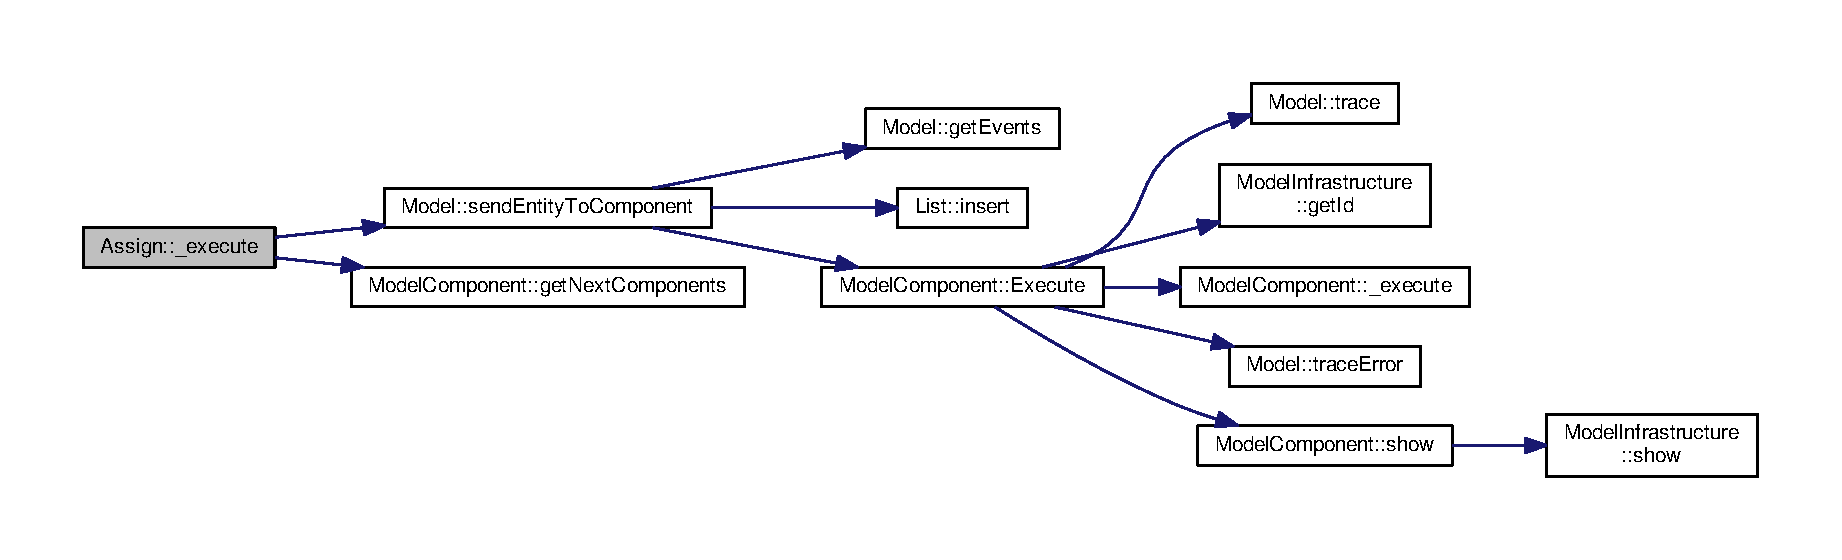
\includegraphics[width=350pt]{class_assign_a5fabf69268b2e65d8b01ce247be87a40_cgraph}
\end{center}
\end{figure}


\hypertarget{class_assign_a47728ac75ef40025f00cca46e04dd012}{\index{Assign@{Assign}!\-\_\-read\-Component@{\-\_\-read\-Component}}
\index{\-\_\-read\-Component@{\-\_\-read\-Component}!Assign@{Assign}}
\subsubsection[{\-\_\-read\-Component}]{\setlength{\rightskip}{0pt plus 5cm}void Assign\-::\-\_\-read\-Component (
\begin{DoxyParamCaption}
\item[{std\-::list$<$ std\-::string $>$}]{words}
\end{DoxyParamCaption}
)\hspace{0.3cm}{\ttfamily [protected]}, {\ttfamily [virtual]}}}\label{class_assign_a47728ac75ef40025f00cca46e04dd012}


Implements \hyperlink{class_model_component_aa16546b209d8fda2c8fa951e88652973}{Model\-Component}.

\hypertarget{class_assign_a5f3a7d8a7214574fea926cae1b1acb94}{\index{Assign@{Assign}!\-\_\-verify\-Symbols@{\-\_\-verify\-Symbols}}
\index{\-\_\-verify\-Symbols@{\-\_\-verify\-Symbols}!Assign@{Assign}}
\subsubsection[{\-\_\-verify\-Symbols}]{\setlength{\rightskip}{0pt plus 5cm}bool Assign\-::\-\_\-verify\-Symbols (
\begin{DoxyParamCaption}
\item[{std\-::string $\ast$}]{error\-Message}
\end{DoxyParamCaption}
)\hspace{0.3cm}{\ttfamily [protected]}, {\ttfamily [virtual]}}}\label{class_assign_a5f3a7d8a7214574fea926cae1b1acb94}


Implements \hyperlink{class_model_component_a183696468482133b2a09b761b7770521}{Model\-Component}.

\hypertarget{class_assign_a6231f1e819d6baab3c9af142fd5b566a}{\index{Assign@{Assign}!\-\_\-write\-Component@{\-\_\-write\-Component}}
\index{\-\_\-write\-Component@{\-\_\-write\-Component}!Assign@{Assign}}
\subsubsection[{\-\_\-write\-Component}]{\setlength{\rightskip}{0pt plus 5cm}std\-::list$<$ std\-::string $>$ $\ast$ Assign\-::\-\_\-write\-Component (
\begin{DoxyParamCaption}
{}
\end{DoxyParamCaption}
)\hspace{0.3cm}{\ttfamily [protected]}, {\ttfamily [virtual]}}}\label{class_assign_a6231f1e819d6baab3c9af142fd5b566a}


Implements \hyperlink{class_model_component_a5847971e860713d9df3e41c603c772c0}{Model\-Component}.

\hypertarget{class_assign_af5022b92204adcd9ee3e444b7e316d07}{\index{Assign@{Assign}!show@{show}}
\index{show@{show}!Assign@{Assign}}
\subsubsection[{show}]{\setlength{\rightskip}{0pt plus 5cm}std\-::string Assign\-::show (
\begin{DoxyParamCaption}
{}
\end{DoxyParamCaption}
)\hspace{0.3cm}{\ttfamily [virtual]}}}\label{class_assign_af5022b92204adcd9ee3e444b7e316d07}


Reimplemented from \hyperlink{class_model_component_ad8bc846e36b028eab7efb7da6c549eca}{Model\-Component}.



Here is the call graph for this function\-:\nopagebreak
\begin{figure}[H]
\begin{center}
\leavevmode
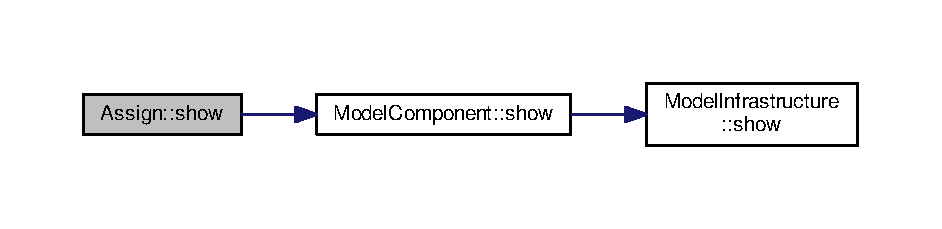
\includegraphics[width=350pt]{class_assign_af5022b92204adcd9ee3e444b7e316d07_cgraph}
\end{center}
\end{figure}




The documentation for this class was generated from the following files\-:\begin{DoxyCompactItemize}
\item 
\hyperlink{_assign_8h}{Assign.\-h}\item 
\hyperlink{_assign_8cpp}{Assign.\-cpp}\end{DoxyCompactItemize}

\hypertarget{class_attribute_value}{\section{Attribute\-Value Class Reference}
\label{class_attribute_value}\index{Attribute\-Value@{Attribute\-Value}}
}


{\ttfamily \#include $<$Attribute\-Value.\-h$>$}

\subsection*{Public Member Functions}
\begin{DoxyCompactItemize}
\item 
\hyperlink{class_attribute_value_a85fc10d30887464438324f511e415e04}{Attribute\-Value} ()
\item 
\hyperlink{class_attribute_value_a5992624b7267bf5e140edeee7181e79d}{Attribute\-Value} (const \hyperlink{class_attribute_value}{Attribute\-Value} \&orig)
\item 
virtual \hyperlink{class_attribute_value_a9d006ff00e58352efcdbc7c86b16a6df}{$\sim$\-Attribute\-Value} ()
\item 
void \hyperlink{class_attribute_value_a2289ac6979d8f6c1dfb1b3998f6f3665}{set\-Value} (double value)
\item 
double \hyperlink{class_attribute_value_a3516a35dd1c503eb73d73082c5c4d36c}{get\-Value} () const 
\end{DoxyCompactItemize}


\subsection{Constructor \& Destructor Documentation}
\hypertarget{class_attribute_value_a85fc10d30887464438324f511e415e04}{\index{Attribute\-Value@{Attribute\-Value}!Attribute\-Value@{Attribute\-Value}}
\index{Attribute\-Value@{Attribute\-Value}!AttributeValue@{Attribute\-Value}}
\subsubsection[{Attribute\-Value}]{\setlength{\rightskip}{0pt plus 5cm}Attribute\-Value\-::\-Attribute\-Value (
\begin{DoxyParamCaption}
{}
\end{DoxyParamCaption}
)}}\label{class_attribute_value_a85fc10d30887464438324f511e415e04}
\hypertarget{class_attribute_value_a5992624b7267bf5e140edeee7181e79d}{\index{Attribute\-Value@{Attribute\-Value}!Attribute\-Value@{Attribute\-Value}}
\index{Attribute\-Value@{Attribute\-Value}!AttributeValue@{Attribute\-Value}}
\subsubsection[{Attribute\-Value}]{\setlength{\rightskip}{0pt plus 5cm}Attribute\-Value\-::\-Attribute\-Value (
\begin{DoxyParamCaption}
\item[{const {\bf Attribute\-Value} \&}]{orig}
\end{DoxyParamCaption}
)}}\label{class_attribute_value_a5992624b7267bf5e140edeee7181e79d}
\hypertarget{class_attribute_value_a9d006ff00e58352efcdbc7c86b16a6df}{\index{Attribute\-Value@{Attribute\-Value}!$\sim$\-Attribute\-Value@{$\sim$\-Attribute\-Value}}
\index{$\sim$\-Attribute\-Value@{$\sim$\-Attribute\-Value}!AttributeValue@{Attribute\-Value}}
\subsubsection[{$\sim$\-Attribute\-Value}]{\setlength{\rightskip}{0pt plus 5cm}Attribute\-Value\-::$\sim$\-Attribute\-Value (
\begin{DoxyParamCaption}
{}
\end{DoxyParamCaption}
)\hspace{0.3cm}{\ttfamily [virtual]}}}\label{class_attribute_value_a9d006ff00e58352efcdbc7c86b16a6df}


\subsection{Member Function Documentation}
\hypertarget{class_attribute_value_a3516a35dd1c503eb73d73082c5c4d36c}{\index{Attribute\-Value@{Attribute\-Value}!get\-Value@{get\-Value}}
\index{get\-Value@{get\-Value}!AttributeValue@{Attribute\-Value}}
\subsubsection[{get\-Value}]{\setlength{\rightskip}{0pt plus 5cm}double Attribute\-Value\-::get\-Value (
\begin{DoxyParamCaption}
{}
\end{DoxyParamCaption}
) const}}\label{class_attribute_value_a3516a35dd1c503eb73d73082c5c4d36c}
\hypertarget{class_attribute_value_a2289ac6979d8f6c1dfb1b3998f6f3665}{\index{Attribute\-Value@{Attribute\-Value}!set\-Value@{set\-Value}}
\index{set\-Value@{set\-Value}!AttributeValue@{Attribute\-Value}}
\subsubsection[{set\-Value}]{\setlength{\rightskip}{0pt plus 5cm}void Attribute\-Value\-::set\-Value (
\begin{DoxyParamCaption}
\item[{double}]{value}
\end{DoxyParamCaption}
)}}\label{class_attribute_value_a2289ac6979d8f6c1dfb1b3998f6f3665}


The documentation for this class was generated from the following files\-:\begin{DoxyCompactItemize}
\item 
\hyperlink{_attribute_value_8h}{Attribute\-Value.\-h}\item 
\hyperlink{_attribute_value_8cpp}{Attribute\-Value.\-cpp}\end{DoxyCompactItemize}

\hypertarget{class_collector__if}{\section{Collector\-\_\-if Class Reference}
\label{class_collector__if}\index{Collector\-\_\-if@{Collector\-\_\-if}}
}


{\ttfamily \#include $<$Collector\-\_\-if.\-h$>$}



Inheritance diagram for Collector\-\_\-if\-:\nopagebreak
\begin{figure}[H]
\begin{center}
\leavevmode
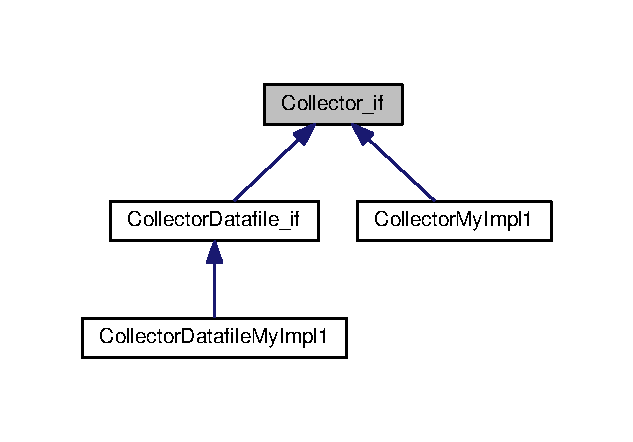
\includegraphics[width=304pt]{class_collector__if__inherit__graph}
\end{center}
\end{figure}
\subsection*{Public Member Functions}
\begin{DoxyCompactItemize}
\item 
virtual void \hyperlink{class_collector__if_a035bd1300c85866870c2f6178a9528e8}{clear} ()=0
\item 
virtual void \hyperlink{class_collector__if_ac7b83bce8ddb4903d247c1eddd656171}{add\-Value} (double value)=0
\item 
virtual double \hyperlink{class_collector__if_aa14f7e1065af8fd38ab592e224fb7e43}{get\-Last\-Value} ()=0
\item 
virtual unsigned int \hyperlink{class_collector__if_a75c20c68c54089105ca8c440997a7cca}{num\-Elements} ()=0
\end{DoxyCompactItemize}


\subsection{Detailed Description}
Interface for collecting values of a single stochastic variable. Values collected can be used as base for statistical analysis. 

\subsection{Member Function Documentation}
\hypertarget{class_collector__if_ac7b83bce8ddb4903d247c1eddd656171}{\index{Collector\-\_\-if@{Collector\-\_\-if}!add\-Value@{add\-Value}}
\index{add\-Value@{add\-Value}!Collector_if@{Collector\-\_\-if}}
\subsubsection[{add\-Value}]{\setlength{\rightskip}{0pt plus 5cm}virtual void Collector\-\_\-if\-::add\-Value (
\begin{DoxyParamCaption}
\item[{double}]{value}
\end{DoxyParamCaption}
)\hspace{0.3cm}{\ttfamily [pure virtual]}}}\label{class_collector__if_ac7b83bce8ddb4903d247c1eddd656171}


Implemented in \hyperlink{class_collector_my_impl1_acc5d658a3429af8b7d4265cbc37485b5}{Collector\-My\-Impl1}, and \hyperlink{class_collector_datafile_my_impl1_aa909fc87f2ee082512616840c9031365}{Collector\-Datafile\-My\-Impl1}.

\hypertarget{class_collector__if_a035bd1300c85866870c2f6178a9528e8}{\index{Collector\-\_\-if@{Collector\-\_\-if}!clear@{clear}}
\index{clear@{clear}!Collector_if@{Collector\-\_\-if}}
\subsubsection[{clear}]{\setlength{\rightskip}{0pt plus 5cm}virtual void Collector\-\_\-if\-::clear (
\begin{DoxyParamCaption}
{}
\end{DoxyParamCaption}
)\hspace{0.3cm}{\ttfamily [pure virtual]}}}\label{class_collector__if_a035bd1300c85866870c2f6178a9528e8}


Implemented in \hyperlink{class_collector_my_impl1_a9b570931955cafde878d6734aa914039}{Collector\-My\-Impl1}, and \hyperlink{class_collector_datafile_my_impl1_a594004f005db5dd1122946445f4db70d}{Collector\-Datafile\-My\-Impl1}.

\hypertarget{class_collector__if_aa14f7e1065af8fd38ab592e224fb7e43}{\index{Collector\-\_\-if@{Collector\-\_\-if}!get\-Last\-Value@{get\-Last\-Value}}
\index{get\-Last\-Value@{get\-Last\-Value}!Collector_if@{Collector\-\_\-if}}
\subsubsection[{get\-Last\-Value}]{\setlength{\rightskip}{0pt plus 5cm}virtual double Collector\-\_\-if\-::get\-Last\-Value (
\begin{DoxyParamCaption}
{}
\end{DoxyParamCaption}
)\hspace{0.3cm}{\ttfamily [pure virtual]}}}\label{class_collector__if_aa14f7e1065af8fd38ab592e224fb7e43}


Implemented in \hyperlink{class_collector_my_impl1_a56e754ba3175e2f335290e2a737e7104}{Collector\-My\-Impl1}, and \hyperlink{class_collector_datafile_my_impl1_a5a29b2f71a4630c658fb83c047fb1054}{Collector\-Datafile\-My\-Impl1}.

\hypertarget{class_collector__if_a75c20c68c54089105ca8c440997a7cca}{\index{Collector\-\_\-if@{Collector\-\_\-if}!num\-Elements@{num\-Elements}}
\index{num\-Elements@{num\-Elements}!Collector_if@{Collector\-\_\-if}}
\subsubsection[{num\-Elements}]{\setlength{\rightskip}{0pt plus 5cm}virtual unsigned int Collector\-\_\-if\-::num\-Elements (
\begin{DoxyParamCaption}
{}
\end{DoxyParamCaption}
)\hspace{0.3cm}{\ttfamily [pure virtual]}}}\label{class_collector__if_a75c20c68c54089105ca8c440997a7cca}


Implemented in \hyperlink{class_collector_my_impl1_ac71aac361d3c9a5d0c9cc76c1c75e47e}{Collector\-My\-Impl1}, and \hyperlink{class_collector_datafile_my_impl1_a6e20d49a94f677a7483412b8d9689950}{Collector\-Datafile\-My\-Impl1}.



The documentation for this class was generated from the following file\-:\begin{DoxyCompactItemize}
\item 
\hyperlink{_collector__if_8h}{Collector\-\_\-if.\-h}\end{DoxyCompactItemize}

\hypertarget{class_collector_datafile__if}{\section{Collector\-Datafile\-\_\-if Class Reference}
\label{class_collector_datafile__if}\index{Collector\-Datafile\-\_\-if@{Collector\-Datafile\-\_\-if}}
}


{\ttfamily \#include $<$Collector\-Datafile\-\_\-if.\-h$>$}



Inheritance diagram for Collector\-Datafile\-\_\-if\-:\nopagebreak
\begin{figure}[H]
\begin{center}
\leavevmode
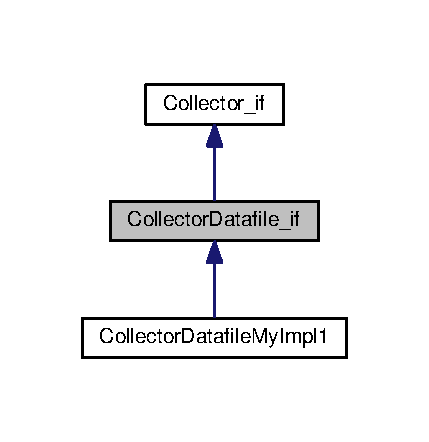
\includegraphics[width=206pt]{class_collector_datafile__if__inherit__graph}
\end{center}
\end{figure}


Collaboration diagram for Collector\-Datafile\-\_\-if\-:\nopagebreak
\begin{figure}[H]
\begin{center}
\leavevmode
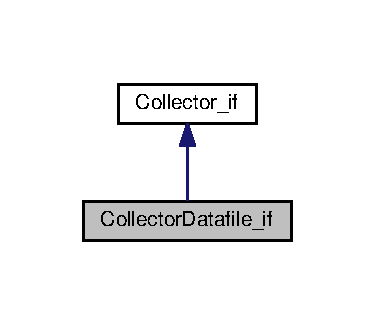
\includegraphics[width=180pt]{class_collector_datafile__if__coll__graph}
\end{center}
\end{figure}
\subsection*{Public Member Functions}
\begin{DoxyCompactItemize}
\item 
virtual double \hyperlink{class_collector_datafile__if_aa790efe68dfa16cebd66b481bbda8411}{get\-Value} (unsigned int num)=0
\item 
virtual std\-::string \hyperlink{class_collector_datafile__if_a81d109f34c25f5295f76ba13f4234a3c}{get\-Data\-Filename} ()=0
\item 
virtual void \hyperlink{class_collector_datafile__if_ab826bbf5472a5cfdbf2f2c30273da8eb}{set\-Data\-Filename} (std\-::string filename)=0
\end{DoxyCompactItemize}


\subsection{Detailed Description}
Interface for collecting values of a stochastic variable that will be stores in a datafile. 

\subsection{Member Function Documentation}
\hypertarget{class_collector_datafile__if_a81d109f34c25f5295f76ba13f4234a3c}{\index{Collector\-Datafile\-\_\-if@{Collector\-Datafile\-\_\-if}!get\-Data\-Filename@{get\-Data\-Filename}}
\index{get\-Data\-Filename@{get\-Data\-Filename}!CollectorDatafile_if@{Collector\-Datafile\-\_\-if}}
\subsubsection[{get\-Data\-Filename}]{\setlength{\rightskip}{0pt plus 5cm}virtual std\-::string Collector\-Datafile\-\_\-if\-::get\-Data\-Filename (
\begin{DoxyParamCaption}
{}
\end{DoxyParamCaption}
)\hspace{0.3cm}{\ttfamily [pure virtual]}}}\label{class_collector_datafile__if_a81d109f34c25f5295f76ba13f4234a3c}


Implemented in \hyperlink{class_collector_datafile_my_impl1_a5ebe8076b9eb9816a1b7d823943102cf}{Collector\-Datafile\-My\-Impl1}.

\hypertarget{class_collector_datafile__if_aa790efe68dfa16cebd66b481bbda8411}{\index{Collector\-Datafile\-\_\-if@{Collector\-Datafile\-\_\-if}!get\-Value@{get\-Value}}
\index{get\-Value@{get\-Value}!CollectorDatafile_if@{Collector\-Datafile\-\_\-if}}
\subsubsection[{get\-Value}]{\setlength{\rightskip}{0pt plus 5cm}virtual double Collector\-Datafile\-\_\-if\-::get\-Value (
\begin{DoxyParamCaption}
\item[{unsigned int}]{num}
\end{DoxyParamCaption}
)\hspace{0.3cm}{\ttfamily [pure virtual]}}}\label{class_collector_datafile__if_aa790efe68dfa16cebd66b481bbda8411}


Implemented in \hyperlink{class_collector_datafile_my_impl1_a55a505d56f9b95a55473bdf1ab24cffe}{Collector\-Datafile\-My\-Impl1}.

\hypertarget{class_collector_datafile__if_ab826bbf5472a5cfdbf2f2c30273da8eb}{\index{Collector\-Datafile\-\_\-if@{Collector\-Datafile\-\_\-if}!set\-Data\-Filename@{set\-Data\-Filename}}
\index{set\-Data\-Filename@{set\-Data\-Filename}!CollectorDatafile_if@{Collector\-Datafile\-\_\-if}}
\subsubsection[{set\-Data\-Filename}]{\setlength{\rightskip}{0pt plus 5cm}virtual void Collector\-Datafile\-\_\-if\-::set\-Data\-Filename (
\begin{DoxyParamCaption}
\item[{std\-::string}]{filename}
\end{DoxyParamCaption}
)\hspace{0.3cm}{\ttfamily [pure virtual]}}}\label{class_collector_datafile__if_ab826bbf5472a5cfdbf2f2c30273da8eb}


Implemented in \hyperlink{class_collector_datafile_my_impl1_ac4c401ae3cf4ccc723b6b9efa614ccd1}{Collector\-Datafile\-My\-Impl1}.



The documentation for this class was generated from the following file\-:\begin{DoxyCompactItemize}
\item 
\hyperlink{_collector_datafile__if_8h}{Collector\-Datafile\-\_\-if.\-h}\end{DoxyCompactItemize}

\hypertarget{class_collector_datafile_my_impl1}{\section{Collector\-Datafile\-My\-Impl1 Class Reference}
\label{class_collector_datafile_my_impl1}\index{Collector\-Datafile\-My\-Impl1@{Collector\-Datafile\-My\-Impl1}}
}


{\ttfamily \#include $<$Collector\-Datafile\-My\-Impl1.\-h$>$}



Inheritance diagram for Collector\-Datafile\-My\-Impl1\-:\nopagebreak
\begin{figure}[H]
\begin{center}
\leavevmode
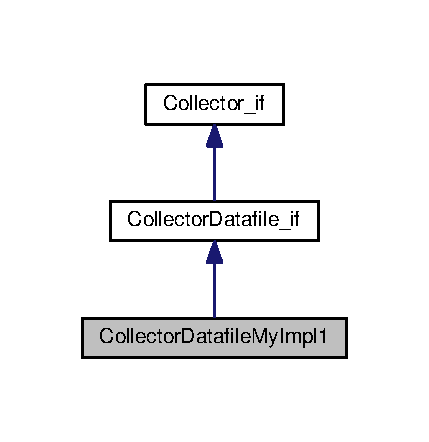
\includegraphics[width=206pt]{class_collector_datafile_my_impl1__inherit__graph}
\end{center}
\end{figure}


Collaboration diagram for Collector\-Datafile\-My\-Impl1\-:\nopagebreak
\begin{figure}[H]
\begin{center}
\leavevmode
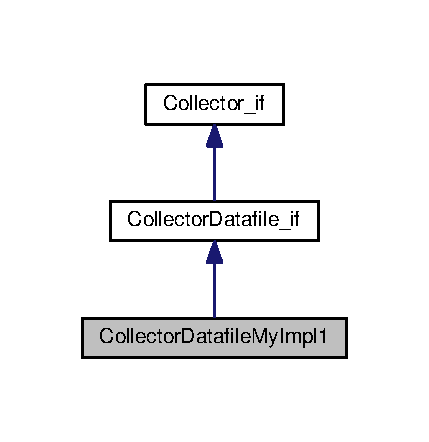
\includegraphics[width=206pt]{class_collector_datafile_my_impl1__coll__graph}
\end{center}
\end{figure}
\subsection*{Public Member Functions}
\begin{DoxyCompactItemize}
\item 
\hyperlink{class_collector_datafile_my_impl1_a88bec096f9b7d707bf436df5b2ab34e1}{Collector\-Datafile\-My\-Impl1} ()
\item 
\hyperlink{class_collector_datafile_my_impl1_a93b68a7b411573a7ff133856f22cbb1f}{Collector\-Datafile\-My\-Impl1} (const \hyperlink{class_collector_datafile_my_impl1}{Collector\-Datafile\-My\-Impl1} \&orig)
\item 
\hyperlink{class_collector_datafile_my_impl1_ac7362a33ec9e82bd3298068cc0c1c6f0}{$\sim$\-Collector\-Datafile\-My\-Impl1} ()
\item 
void \hyperlink{class_collector_datafile_my_impl1_a594004f005db5dd1122946445f4db70d}{clear} ()
\item 
void \hyperlink{class_collector_datafile_my_impl1_aa909fc87f2ee082512616840c9031365}{add\-Value} (double value)
\item 
double \hyperlink{class_collector_datafile_my_impl1_a5a29b2f71a4630c658fb83c047fb1054}{get\-Last\-Value} ()
\item 
unsigned int \hyperlink{class_collector_datafile_my_impl1_a6e20d49a94f677a7483412b8d9689950}{num\-Elements} ()
\item 
double \hyperlink{class_collector_datafile_my_impl1_a55a505d56f9b95a55473bdf1ab24cffe}{get\-Value} (unsigned int num)
\item 
std\-::string \hyperlink{class_collector_datafile_my_impl1_a5ebe8076b9eb9816a1b7d823943102cf}{get\-Data\-Filename} ()
\item 
void \hyperlink{class_collector_datafile_my_impl1_ac4c401ae3cf4ccc723b6b9efa614ccd1}{set\-Data\-Filename} (std\-::string filename)
\end{DoxyCompactItemize}


\subsection{Constructor \& Destructor Documentation}
\hypertarget{class_collector_datafile_my_impl1_a88bec096f9b7d707bf436df5b2ab34e1}{\index{Collector\-Datafile\-My\-Impl1@{Collector\-Datafile\-My\-Impl1}!Collector\-Datafile\-My\-Impl1@{Collector\-Datafile\-My\-Impl1}}
\index{Collector\-Datafile\-My\-Impl1@{Collector\-Datafile\-My\-Impl1}!CollectorDatafileMyImpl1@{Collector\-Datafile\-My\-Impl1}}
\subsubsection[{Collector\-Datafile\-My\-Impl1}]{\setlength{\rightskip}{0pt plus 5cm}Collector\-Datafile\-My\-Impl1\-::\-Collector\-Datafile\-My\-Impl1 (
\begin{DoxyParamCaption}
{}
\end{DoxyParamCaption}
)}}\label{class_collector_datafile_my_impl1_a88bec096f9b7d707bf436df5b2ab34e1}
\hypertarget{class_collector_datafile_my_impl1_a93b68a7b411573a7ff133856f22cbb1f}{\index{Collector\-Datafile\-My\-Impl1@{Collector\-Datafile\-My\-Impl1}!Collector\-Datafile\-My\-Impl1@{Collector\-Datafile\-My\-Impl1}}
\index{Collector\-Datafile\-My\-Impl1@{Collector\-Datafile\-My\-Impl1}!CollectorDatafileMyImpl1@{Collector\-Datafile\-My\-Impl1}}
\subsubsection[{Collector\-Datafile\-My\-Impl1}]{\setlength{\rightskip}{0pt plus 5cm}Collector\-Datafile\-My\-Impl1\-::\-Collector\-Datafile\-My\-Impl1 (
\begin{DoxyParamCaption}
\item[{const {\bf Collector\-Datafile\-My\-Impl1} \&}]{orig}
\end{DoxyParamCaption}
)}}\label{class_collector_datafile_my_impl1_a93b68a7b411573a7ff133856f22cbb1f}
\hypertarget{class_collector_datafile_my_impl1_ac7362a33ec9e82bd3298068cc0c1c6f0}{\index{Collector\-Datafile\-My\-Impl1@{Collector\-Datafile\-My\-Impl1}!$\sim$\-Collector\-Datafile\-My\-Impl1@{$\sim$\-Collector\-Datafile\-My\-Impl1}}
\index{$\sim$\-Collector\-Datafile\-My\-Impl1@{$\sim$\-Collector\-Datafile\-My\-Impl1}!CollectorDatafileMyImpl1@{Collector\-Datafile\-My\-Impl1}}
\subsubsection[{$\sim$\-Collector\-Datafile\-My\-Impl1}]{\setlength{\rightskip}{0pt plus 5cm}Collector\-Datafile\-My\-Impl1\-::$\sim$\-Collector\-Datafile\-My\-Impl1 (
\begin{DoxyParamCaption}
{}
\end{DoxyParamCaption}
)}}\label{class_collector_datafile_my_impl1_ac7362a33ec9e82bd3298068cc0c1c6f0}


\subsection{Member Function Documentation}
\hypertarget{class_collector_datafile_my_impl1_aa909fc87f2ee082512616840c9031365}{\index{Collector\-Datafile\-My\-Impl1@{Collector\-Datafile\-My\-Impl1}!add\-Value@{add\-Value}}
\index{add\-Value@{add\-Value}!CollectorDatafileMyImpl1@{Collector\-Datafile\-My\-Impl1}}
\subsubsection[{add\-Value}]{\setlength{\rightskip}{0pt plus 5cm}void Collector\-Datafile\-My\-Impl1\-::add\-Value (
\begin{DoxyParamCaption}
\item[{double}]{value}
\end{DoxyParamCaption}
)\hspace{0.3cm}{\ttfamily [virtual]}}}\label{class_collector_datafile_my_impl1_aa909fc87f2ee082512616840c9031365}


Implements \hyperlink{class_collector__if_ac7b83bce8ddb4903d247c1eddd656171}{Collector\-\_\-if}.

\hypertarget{class_collector_datafile_my_impl1_a594004f005db5dd1122946445f4db70d}{\index{Collector\-Datafile\-My\-Impl1@{Collector\-Datafile\-My\-Impl1}!clear@{clear}}
\index{clear@{clear}!CollectorDatafileMyImpl1@{Collector\-Datafile\-My\-Impl1}}
\subsubsection[{clear}]{\setlength{\rightskip}{0pt plus 5cm}void Collector\-Datafile\-My\-Impl1\-::clear (
\begin{DoxyParamCaption}
{}
\end{DoxyParamCaption}
)\hspace{0.3cm}{\ttfamily [virtual]}}}\label{class_collector_datafile_my_impl1_a594004f005db5dd1122946445f4db70d}


Implements \hyperlink{class_collector__if_a035bd1300c85866870c2f6178a9528e8}{Collector\-\_\-if}.

\hypertarget{class_collector_datafile_my_impl1_a5ebe8076b9eb9816a1b7d823943102cf}{\index{Collector\-Datafile\-My\-Impl1@{Collector\-Datafile\-My\-Impl1}!get\-Data\-Filename@{get\-Data\-Filename}}
\index{get\-Data\-Filename@{get\-Data\-Filename}!CollectorDatafileMyImpl1@{Collector\-Datafile\-My\-Impl1}}
\subsubsection[{get\-Data\-Filename}]{\setlength{\rightskip}{0pt plus 5cm}std\-::string Collector\-Datafile\-My\-Impl1\-::get\-Data\-Filename (
\begin{DoxyParamCaption}
{}
\end{DoxyParamCaption}
)\hspace{0.3cm}{\ttfamily [virtual]}}}\label{class_collector_datafile_my_impl1_a5ebe8076b9eb9816a1b7d823943102cf}


Implements \hyperlink{class_collector_datafile__if_a81d109f34c25f5295f76ba13f4234a3c}{Collector\-Datafile\-\_\-if}.

\hypertarget{class_collector_datafile_my_impl1_a5a29b2f71a4630c658fb83c047fb1054}{\index{Collector\-Datafile\-My\-Impl1@{Collector\-Datafile\-My\-Impl1}!get\-Last\-Value@{get\-Last\-Value}}
\index{get\-Last\-Value@{get\-Last\-Value}!CollectorDatafileMyImpl1@{Collector\-Datafile\-My\-Impl1}}
\subsubsection[{get\-Last\-Value}]{\setlength{\rightskip}{0pt plus 5cm}double Collector\-Datafile\-My\-Impl1\-::get\-Last\-Value (
\begin{DoxyParamCaption}
{}
\end{DoxyParamCaption}
)\hspace{0.3cm}{\ttfamily [virtual]}}}\label{class_collector_datafile_my_impl1_a5a29b2f71a4630c658fb83c047fb1054}


Implements \hyperlink{class_collector__if_aa14f7e1065af8fd38ab592e224fb7e43}{Collector\-\_\-if}.

\hypertarget{class_collector_datafile_my_impl1_a55a505d56f9b95a55473bdf1ab24cffe}{\index{Collector\-Datafile\-My\-Impl1@{Collector\-Datafile\-My\-Impl1}!get\-Value@{get\-Value}}
\index{get\-Value@{get\-Value}!CollectorDatafileMyImpl1@{Collector\-Datafile\-My\-Impl1}}
\subsubsection[{get\-Value}]{\setlength{\rightskip}{0pt plus 5cm}double Collector\-Datafile\-My\-Impl1\-::get\-Value (
\begin{DoxyParamCaption}
\item[{unsigned int}]{num}
\end{DoxyParamCaption}
)\hspace{0.3cm}{\ttfamily [virtual]}}}\label{class_collector_datafile_my_impl1_a55a505d56f9b95a55473bdf1ab24cffe}


Implements \hyperlink{class_collector_datafile__if_aa790efe68dfa16cebd66b481bbda8411}{Collector\-Datafile\-\_\-if}.

\hypertarget{class_collector_datafile_my_impl1_a6e20d49a94f677a7483412b8d9689950}{\index{Collector\-Datafile\-My\-Impl1@{Collector\-Datafile\-My\-Impl1}!num\-Elements@{num\-Elements}}
\index{num\-Elements@{num\-Elements}!CollectorDatafileMyImpl1@{Collector\-Datafile\-My\-Impl1}}
\subsubsection[{num\-Elements}]{\setlength{\rightskip}{0pt plus 5cm}unsigned int Collector\-Datafile\-My\-Impl1\-::num\-Elements (
\begin{DoxyParamCaption}
{}
\end{DoxyParamCaption}
)\hspace{0.3cm}{\ttfamily [virtual]}}}\label{class_collector_datafile_my_impl1_a6e20d49a94f677a7483412b8d9689950}


Implements \hyperlink{class_collector__if_a75c20c68c54089105ca8c440997a7cca}{Collector\-\_\-if}.

\hypertarget{class_collector_datafile_my_impl1_ac4c401ae3cf4ccc723b6b9efa614ccd1}{\index{Collector\-Datafile\-My\-Impl1@{Collector\-Datafile\-My\-Impl1}!set\-Data\-Filename@{set\-Data\-Filename}}
\index{set\-Data\-Filename@{set\-Data\-Filename}!CollectorDatafileMyImpl1@{Collector\-Datafile\-My\-Impl1}}
\subsubsection[{set\-Data\-Filename}]{\setlength{\rightskip}{0pt plus 5cm}void Collector\-Datafile\-My\-Impl1\-::set\-Data\-Filename (
\begin{DoxyParamCaption}
\item[{std\-::string}]{filename}
\end{DoxyParamCaption}
)\hspace{0.3cm}{\ttfamily [virtual]}}}\label{class_collector_datafile_my_impl1_ac4c401ae3cf4ccc723b6b9efa614ccd1}


Implements \hyperlink{class_collector_datafile__if_ab826bbf5472a5cfdbf2f2c30273da8eb}{Collector\-Datafile\-\_\-if}.



The documentation for this class was generated from the following files\-:\begin{DoxyCompactItemize}
\item 
\hyperlink{_collector_datafile_my_impl1_8h}{Collector\-Datafile\-My\-Impl1.\-h}\item 
\hyperlink{_collector_datafile_my_impl1_8cpp}{Collector\-Datafile\-My\-Impl1.\-cpp}\end{DoxyCompactItemize}

\hypertarget{class_collector_my_impl1}{\section{Collector\-My\-Impl1 Class Reference}
\label{class_collector_my_impl1}\index{Collector\-My\-Impl1@{Collector\-My\-Impl1}}
}


{\ttfamily \#include $<$Collector\-My\-Impl1.\-h$>$}



Inheritance diagram for Collector\-My\-Impl1\-:\nopagebreak
\begin{figure}[H]
\begin{center}
\leavevmode
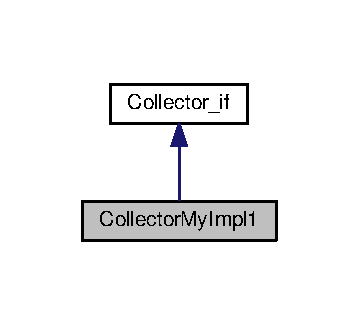
\includegraphics[width=172pt]{class_collector_my_impl1__inherit__graph}
\end{center}
\end{figure}


Collaboration diagram for Collector\-My\-Impl1\-:\nopagebreak
\begin{figure}[H]
\begin{center}
\leavevmode
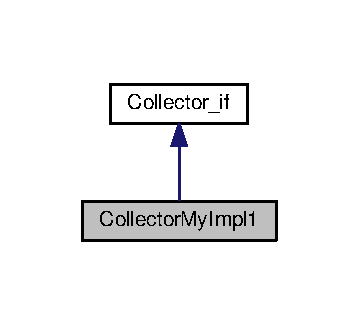
\includegraphics[width=172pt]{class_collector_my_impl1__coll__graph}
\end{center}
\end{figure}
\subsection*{Public Member Functions}
\begin{DoxyCompactItemize}
\item 
\hyperlink{class_collector_my_impl1_ab8d5d86d5d28f0cc3a4558fe5a6da56c}{Collector\-My\-Impl1} ()
\item 
\hyperlink{class_collector_my_impl1_a7d96fa7024ff2e2158613c4b55ea052f}{Collector\-My\-Impl1} (const \hyperlink{class_collector_my_impl1}{Collector\-My\-Impl1} \&orig)
\item 
\hyperlink{class_collector_my_impl1_a431e418b9b2cf55e6fb10ba688ae281e}{$\sim$\-Collector\-My\-Impl1} ()
\item 
void \hyperlink{class_collector_my_impl1_a9b570931955cafde878d6734aa914039}{clear} ()
\item 
void \hyperlink{class_collector_my_impl1_acc5d658a3429af8b7d4265cbc37485b5}{add\-Value} (double value)
\item 
double \hyperlink{class_collector_my_impl1_a56e754ba3175e2f335290e2a737e7104}{get\-Last\-Value} ()
\item 
unsigned int \hyperlink{class_collector_my_impl1_ac71aac361d3c9a5d0c9cc76c1c75e47e}{num\-Elements} ()
\end{DoxyCompactItemize}


\subsection{Constructor \& Destructor Documentation}
\hypertarget{class_collector_my_impl1_ab8d5d86d5d28f0cc3a4558fe5a6da56c}{\index{Collector\-My\-Impl1@{Collector\-My\-Impl1}!Collector\-My\-Impl1@{Collector\-My\-Impl1}}
\index{Collector\-My\-Impl1@{Collector\-My\-Impl1}!CollectorMyImpl1@{Collector\-My\-Impl1}}
\subsubsection[{Collector\-My\-Impl1}]{\setlength{\rightskip}{0pt plus 5cm}Collector\-My\-Impl1\-::\-Collector\-My\-Impl1 (
\begin{DoxyParamCaption}
{}
\end{DoxyParamCaption}
)}}\label{class_collector_my_impl1_ab8d5d86d5d28f0cc3a4558fe5a6da56c}
\hypertarget{class_collector_my_impl1_a7d96fa7024ff2e2158613c4b55ea052f}{\index{Collector\-My\-Impl1@{Collector\-My\-Impl1}!Collector\-My\-Impl1@{Collector\-My\-Impl1}}
\index{Collector\-My\-Impl1@{Collector\-My\-Impl1}!CollectorMyImpl1@{Collector\-My\-Impl1}}
\subsubsection[{Collector\-My\-Impl1}]{\setlength{\rightskip}{0pt plus 5cm}Collector\-My\-Impl1\-::\-Collector\-My\-Impl1 (
\begin{DoxyParamCaption}
\item[{const {\bf Collector\-My\-Impl1} \&}]{orig}
\end{DoxyParamCaption}
)}}\label{class_collector_my_impl1_a7d96fa7024ff2e2158613c4b55ea052f}
\hypertarget{class_collector_my_impl1_a431e418b9b2cf55e6fb10ba688ae281e}{\index{Collector\-My\-Impl1@{Collector\-My\-Impl1}!$\sim$\-Collector\-My\-Impl1@{$\sim$\-Collector\-My\-Impl1}}
\index{$\sim$\-Collector\-My\-Impl1@{$\sim$\-Collector\-My\-Impl1}!CollectorMyImpl1@{Collector\-My\-Impl1}}
\subsubsection[{$\sim$\-Collector\-My\-Impl1}]{\setlength{\rightskip}{0pt plus 5cm}Collector\-My\-Impl1\-::$\sim$\-Collector\-My\-Impl1 (
\begin{DoxyParamCaption}
{}
\end{DoxyParamCaption}
)}}\label{class_collector_my_impl1_a431e418b9b2cf55e6fb10ba688ae281e}


\subsection{Member Function Documentation}
\hypertarget{class_collector_my_impl1_acc5d658a3429af8b7d4265cbc37485b5}{\index{Collector\-My\-Impl1@{Collector\-My\-Impl1}!add\-Value@{add\-Value}}
\index{add\-Value@{add\-Value}!CollectorMyImpl1@{Collector\-My\-Impl1}}
\subsubsection[{add\-Value}]{\setlength{\rightskip}{0pt plus 5cm}void Collector\-My\-Impl1\-::add\-Value (
\begin{DoxyParamCaption}
\item[{double}]{value}
\end{DoxyParamCaption}
)\hspace{0.3cm}{\ttfamily [virtual]}}}\label{class_collector_my_impl1_acc5d658a3429af8b7d4265cbc37485b5}


Implements \hyperlink{class_collector__if_ac7b83bce8ddb4903d247c1eddd656171}{Collector\-\_\-if}.

\hypertarget{class_collector_my_impl1_a9b570931955cafde878d6734aa914039}{\index{Collector\-My\-Impl1@{Collector\-My\-Impl1}!clear@{clear}}
\index{clear@{clear}!CollectorMyImpl1@{Collector\-My\-Impl1}}
\subsubsection[{clear}]{\setlength{\rightskip}{0pt plus 5cm}void Collector\-My\-Impl1\-::clear (
\begin{DoxyParamCaption}
{}
\end{DoxyParamCaption}
)\hspace{0.3cm}{\ttfamily [virtual]}}}\label{class_collector_my_impl1_a9b570931955cafde878d6734aa914039}


Implements \hyperlink{class_collector__if_a035bd1300c85866870c2f6178a9528e8}{Collector\-\_\-if}.

\hypertarget{class_collector_my_impl1_a56e754ba3175e2f335290e2a737e7104}{\index{Collector\-My\-Impl1@{Collector\-My\-Impl1}!get\-Last\-Value@{get\-Last\-Value}}
\index{get\-Last\-Value@{get\-Last\-Value}!CollectorMyImpl1@{Collector\-My\-Impl1}}
\subsubsection[{get\-Last\-Value}]{\setlength{\rightskip}{0pt plus 5cm}double Collector\-My\-Impl1\-::get\-Last\-Value (
\begin{DoxyParamCaption}
{}
\end{DoxyParamCaption}
)\hspace{0.3cm}{\ttfamily [virtual]}}}\label{class_collector_my_impl1_a56e754ba3175e2f335290e2a737e7104}


Implements \hyperlink{class_collector__if_aa14f7e1065af8fd38ab592e224fb7e43}{Collector\-\_\-if}.

\hypertarget{class_collector_my_impl1_ac71aac361d3c9a5d0c9cc76c1c75e47e}{\index{Collector\-My\-Impl1@{Collector\-My\-Impl1}!num\-Elements@{num\-Elements}}
\index{num\-Elements@{num\-Elements}!CollectorMyImpl1@{Collector\-My\-Impl1}}
\subsubsection[{num\-Elements}]{\setlength{\rightskip}{0pt plus 5cm}unsigned int Collector\-My\-Impl1\-::num\-Elements (
\begin{DoxyParamCaption}
{}
\end{DoxyParamCaption}
)\hspace{0.3cm}{\ttfamily [virtual]}}}\label{class_collector_my_impl1_ac71aac361d3c9a5d0c9cc76c1c75e47e}


Implements \hyperlink{class_collector__if_a75c20c68c54089105ca8c440997a7cca}{Collector\-\_\-if}.



The documentation for this class was generated from the following files\-:\begin{DoxyCompactItemize}
\item 
\hyperlink{_collector_my_impl1_8h}{Collector\-My\-Impl1.\-h}\item 
\hyperlink{_collector_my_impl1_8cpp}{Collector\-My\-Impl1.\-cpp}\end{DoxyCompactItemize}

\hypertarget{class_create}{\section{Create Class Reference}
\label{class_create}\index{Create@{Create}}
}


{\ttfamily \#include $<$Create.\-h$>$}



Inheritance diagram for Create\-:\nopagebreak
\begin{figure}[H]
\begin{center}
\leavevmode
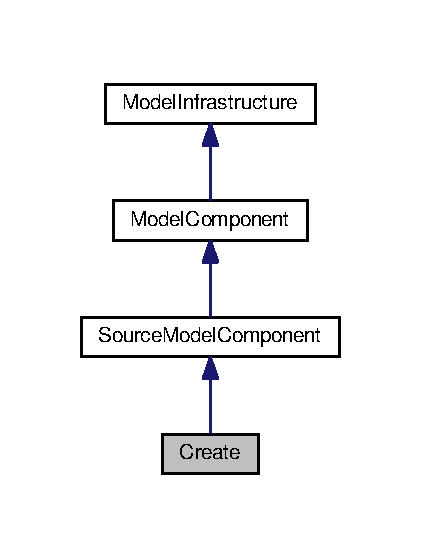
\includegraphics[width=202pt]{class_create__inherit__graph}
\end{center}
\end{figure}


Collaboration diagram for Create\-:\nopagebreak
\begin{figure}[H]
\begin{center}
\leavevmode
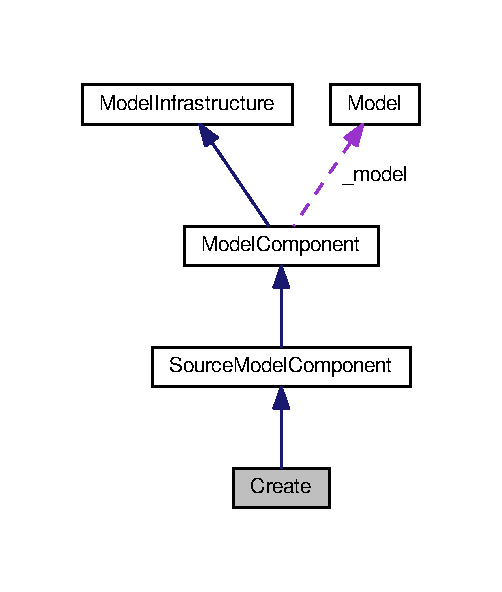
\includegraphics[width=241pt]{class_create__coll__graph}
\end{center}
\end{figure}
\subsection*{Public Member Functions}
\begin{DoxyCompactItemize}
\item 
\hyperlink{class_create_a81bd7a50b926660c264ebe29e2095170}{Create} (\hyperlink{class_model}{Model} $\ast$model)
\item 
\hyperlink{class_create_a035a6f7ddd02dace181b23913b91bad9}{Create} (const \hyperlink{class_create}{Create} \&orig)
\item 
virtual \hyperlink{class_create_a6060fda2b105228446ddddb09f63d127}{$\sim$\-Create} ()
\item 
virtual std\-::string \hyperlink{class_create_a8d1832d2165bbeea4a5a88aded883f86}{show} ()
\end{DoxyCompactItemize}
\subsection*{Protected Member Functions}
\begin{DoxyCompactItemize}
\item 
virtual void \hyperlink{class_create_acd3a4b8805561591e0c88d3fd689cf74}{\-\_\-execute} (\hyperlink{class_entity}{Entity} $\ast$entity)
\item 
virtual void \hyperlink{class_create_afccd427ad3821a95308498892dfe58f3}{\-\_\-read\-Component} (std\-::list$<$ std\-::string $>$ words)
\item 
virtual std\-::list$<$ std\-::string $>$ $\ast$ \hyperlink{class_create_ab0fd0c7afa14e91a82ecd151d22ce20b}{\-\_\-write\-Component} ()
\item 
virtual bool \hyperlink{class_create_ad445fd3bec94b4e66669089f10f96057}{\-\_\-verify\-Symbols} (std\-::string $\ast$error\-Message)
\end{DoxyCompactItemize}
\subsection*{Additional Inherited Members}


\subsection{Detailed Description}
\hyperlink{class_create}{Create} is the most basic component to include the first entities into the model, and therefore is a source component (derived from \hyperlink{class_source_model_component}{Source\-Model\-Component}) 

\subsection{Constructor \& Destructor Documentation}
\hypertarget{class_create_a81bd7a50b926660c264ebe29e2095170}{\index{Create@{Create}!Create@{Create}}
\index{Create@{Create}!Create@{Create}}
\subsubsection[{Create}]{\setlength{\rightskip}{0pt plus 5cm}Create\-::\-Create (
\begin{DoxyParamCaption}
\item[{{\bf Model} $\ast$}]{model}
\end{DoxyParamCaption}
)}}\label{class_create_a81bd7a50b926660c264ebe29e2095170}
\hypertarget{class_create_a035a6f7ddd02dace181b23913b91bad9}{\index{Create@{Create}!Create@{Create}}
\index{Create@{Create}!Create@{Create}}
\subsubsection[{Create}]{\setlength{\rightskip}{0pt plus 5cm}Create\-::\-Create (
\begin{DoxyParamCaption}
\item[{const {\bf Create} \&}]{orig}
\end{DoxyParamCaption}
)}}\label{class_create_a035a6f7ddd02dace181b23913b91bad9}
\hypertarget{class_create_a6060fda2b105228446ddddb09f63d127}{\index{Create@{Create}!$\sim$\-Create@{$\sim$\-Create}}
\index{$\sim$\-Create@{$\sim$\-Create}!Create@{Create}}
\subsubsection[{$\sim$\-Create}]{\setlength{\rightskip}{0pt plus 5cm}Create\-::$\sim$\-Create (
\begin{DoxyParamCaption}
{}
\end{DoxyParamCaption}
)\hspace{0.3cm}{\ttfamily [virtual]}}}\label{class_create_a6060fda2b105228446ddddb09f63d127}


\subsection{Member Function Documentation}
\hypertarget{class_create_acd3a4b8805561591e0c88d3fd689cf74}{\index{Create@{Create}!\-\_\-execute@{\-\_\-execute}}
\index{\-\_\-execute@{\-\_\-execute}!Create@{Create}}
\subsubsection[{\-\_\-execute}]{\setlength{\rightskip}{0pt plus 5cm}void Create\-::\-\_\-execute (
\begin{DoxyParamCaption}
\item[{{\bf Entity} $\ast$}]{entity}
\end{DoxyParamCaption}
)\hspace{0.3cm}{\ttfamily [protected]}, {\ttfamily [virtual]}}}\label{class_create_acd3a4b8805561591e0c88d3fd689cf74}


Implements \hyperlink{class_model_component_ae3fcf8bbdd8368c882438424aa73f714}{Model\-Component}.



Here is the call graph for this function\-:\nopagebreak
\begin{figure}[H]
\begin{center}
\leavevmode
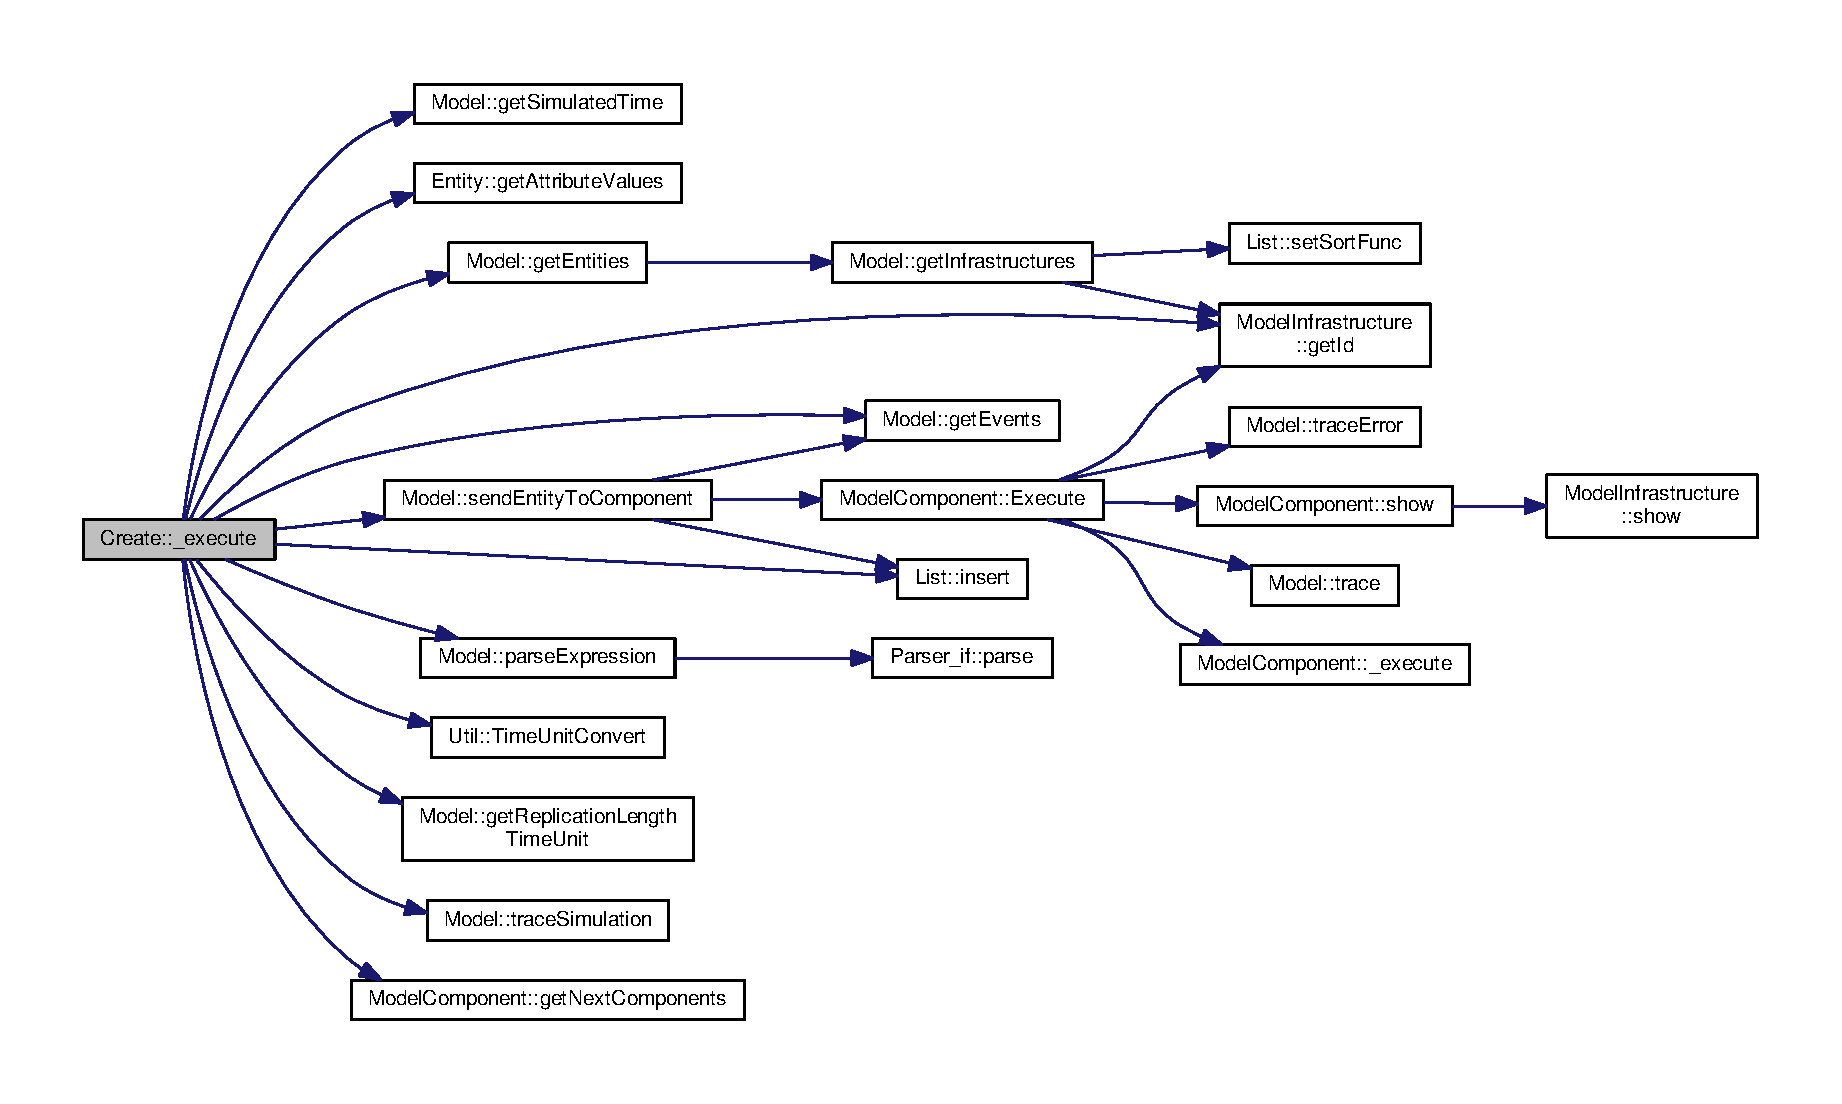
\includegraphics[width=350pt]{class_create_acd3a4b8805561591e0c88d3fd689cf74_cgraph}
\end{center}
\end{figure}


\hypertarget{class_create_afccd427ad3821a95308498892dfe58f3}{\index{Create@{Create}!\-\_\-read\-Component@{\-\_\-read\-Component}}
\index{\-\_\-read\-Component@{\-\_\-read\-Component}!Create@{Create}}
\subsubsection[{\-\_\-read\-Component}]{\setlength{\rightskip}{0pt plus 5cm}void Create\-::\-\_\-read\-Component (
\begin{DoxyParamCaption}
\item[{std\-::list$<$ std\-::string $>$}]{words}
\end{DoxyParamCaption}
)\hspace{0.3cm}{\ttfamily [protected]}, {\ttfamily [virtual]}}}\label{class_create_afccd427ad3821a95308498892dfe58f3}


Implements \hyperlink{class_model_component_aa16546b209d8fda2c8fa951e88652973}{Model\-Component}.

\hypertarget{class_create_ad445fd3bec94b4e66669089f10f96057}{\index{Create@{Create}!\-\_\-verify\-Symbols@{\-\_\-verify\-Symbols}}
\index{\-\_\-verify\-Symbols@{\-\_\-verify\-Symbols}!Create@{Create}}
\subsubsection[{\-\_\-verify\-Symbols}]{\setlength{\rightskip}{0pt plus 5cm}bool Create\-::\-\_\-verify\-Symbols (
\begin{DoxyParamCaption}
\item[{std\-::string $\ast$}]{error\-Message}
\end{DoxyParamCaption}
)\hspace{0.3cm}{\ttfamily [protected]}, {\ttfamily [virtual]}}}\label{class_create_ad445fd3bec94b4e66669089f10f96057}


Implements \hyperlink{class_model_component_a183696468482133b2a09b761b7770521}{Model\-Component}.



Here is the call graph for this function\-:\nopagebreak
\begin{figure}[H]
\begin{center}
\leavevmode
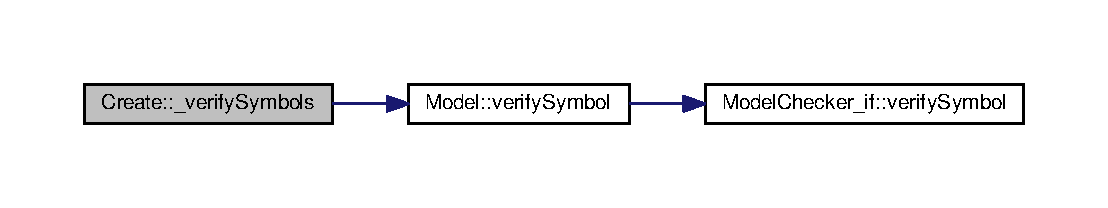
\includegraphics[width=350pt]{class_create_ad445fd3bec94b4e66669089f10f96057_cgraph}
\end{center}
\end{figure}


\hypertarget{class_create_ab0fd0c7afa14e91a82ecd151d22ce20b}{\index{Create@{Create}!\-\_\-write\-Component@{\-\_\-write\-Component}}
\index{\-\_\-write\-Component@{\-\_\-write\-Component}!Create@{Create}}
\subsubsection[{\-\_\-write\-Component}]{\setlength{\rightskip}{0pt plus 5cm}std\-::list$<$ std\-::string $>$ $\ast$ Create\-::\-\_\-write\-Component (
\begin{DoxyParamCaption}
{}
\end{DoxyParamCaption}
)\hspace{0.3cm}{\ttfamily [protected]}, {\ttfamily [virtual]}}}\label{class_create_ab0fd0c7afa14e91a82ecd151d22ce20b}


Implements \hyperlink{class_model_component_a5847971e860713d9df3e41c603c772c0}{Model\-Component}.



Here is the call graph for this function\-:\nopagebreak
\begin{figure}[H]
\begin{center}
\leavevmode
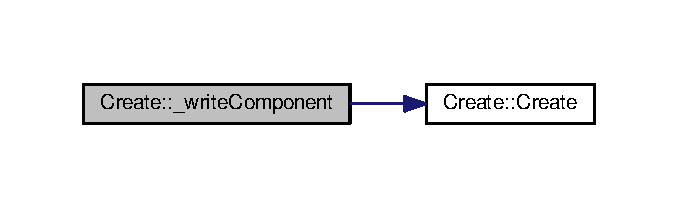
\includegraphics[width=326pt]{class_create_ab0fd0c7afa14e91a82ecd151d22ce20b_cgraph}
\end{center}
\end{figure}


\hypertarget{class_create_a8d1832d2165bbeea4a5a88aded883f86}{\index{Create@{Create}!show@{show}}
\index{show@{show}!Create@{Create}}
\subsubsection[{show}]{\setlength{\rightskip}{0pt plus 5cm}std\-::string Create\-::show (
\begin{DoxyParamCaption}
{}
\end{DoxyParamCaption}
)\hspace{0.3cm}{\ttfamily [virtual]}}}\label{class_create_a8d1832d2165bbeea4a5a88aded883f86}


Reimplemented from \hyperlink{class_source_model_component_a4011597b5780fcc0495e8e22ab8158f6}{Source\-Model\-Component}.



Here is the call graph for this function\-:\nopagebreak
\begin{figure}[H]
\begin{center}
\leavevmode
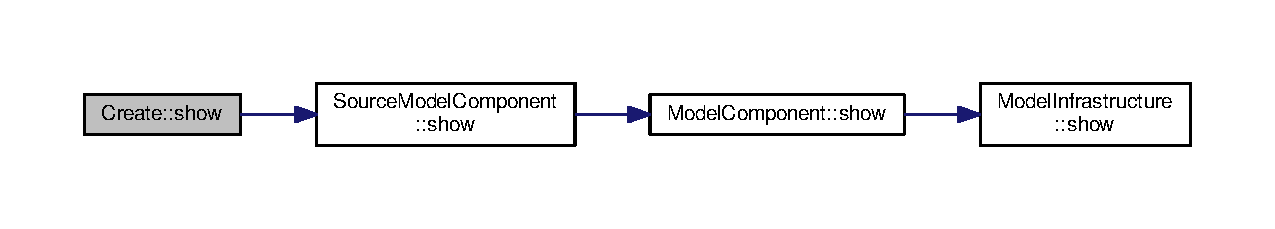
\includegraphics[width=350pt]{class_create_a8d1832d2165bbeea4a5a88aded883f86_cgraph}
\end{center}
\end{figure}




The documentation for this class was generated from the following files\-:\begin{DoxyCompactItemize}
\item 
\hyperlink{_create_8h}{Create.\-h}\item 
\hyperlink{_create_8cpp}{Create.\-cpp}\end{DoxyCompactItemize}

\hypertarget{class_delay}{\section{Delay Class Reference}
\label{class_delay}\index{Delay@{Delay}}
}


{\ttfamily \#include $<$Delay.\-h$>$}



Inheritance diagram for Delay\-:\nopagebreak
\begin{figure}[H]
\begin{center}
\leavevmode
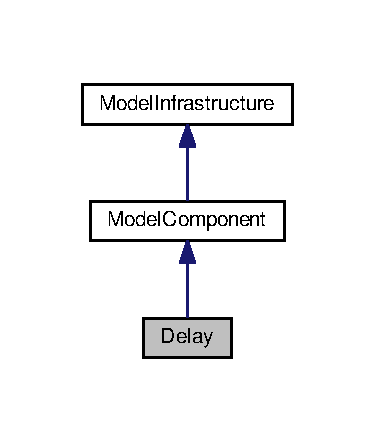
\includegraphics[width=180pt]{class_delay__inherit__graph}
\end{center}
\end{figure}


Collaboration diagram for Delay\-:\nopagebreak
\begin{figure}[H]
\begin{center}
\leavevmode
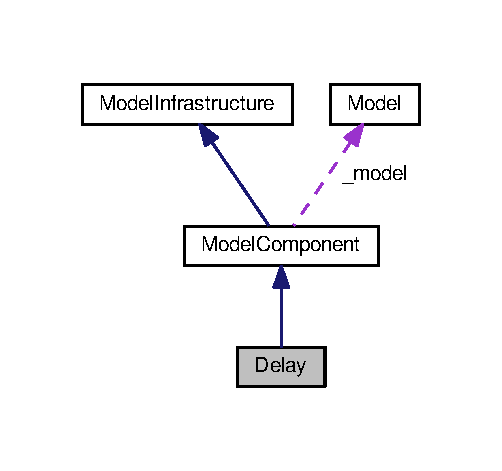
\includegraphics[width=241pt]{class_delay__coll__graph}
\end{center}
\end{figure}
\subsection*{Public Member Functions}
\begin{DoxyCompactItemize}
\item 
\hyperlink{class_delay_a155ad32911b3289d968cca746f940520}{Delay} (\hyperlink{class_model}{Model} $\ast$model)
\item 
\hyperlink{class_delay_a5892fd8feb283f11980c0a9adb9befa7}{Delay} (const \hyperlink{class_delay}{Delay} \&orig)
\item 
virtual \hyperlink{class_delay_afee934130955d45563a6c5baaaf052d2}{$\sim$\-Delay} ()
\item 
void \hyperlink{class_delay_a683b53af607a424477acb946eb3afdfc}{set\-Delay\-Expression} (std\-::string \-\_\-delay\-Expression)
\item 
std\-::string \hyperlink{class_delay_a58559eda9ed25330d29b967c1bb0add5}{get\-Delay\-Expression} () const 
\item 
void \hyperlink{class_delay_abe7e89dba0974a81d00e6d2c0548fc1e}{set\-Delay\-Time\-Unit} (\hyperlink{class_util_aadbd82055afeaa7d4fb4da513de628ff}{Util\-::\-Time\-Unit} \-\_\-delay\-Time\-Unit)
\item 
\hyperlink{class_util_aadbd82055afeaa7d4fb4da513de628ff}{Util\-::\-Time\-Unit} \hyperlink{class_delay_a0561a6fdb4dd317952b5bb8d87b0c15f}{get\-Delay\-Time\-Unit} () const 
\item 
virtual std\-::string \hyperlink{class_delay_af8187e4515417b547dc22b5ee0a1f95d}{show} ()
\end{DoxyCompactItemize}
\subsection*{Protected Member Functions}
\begin{DoxyCompactItemize}
\item 
virtual void \hyperlink{class_delay_a029d91a2cd736ff9c361c69336e6ab41}{\-\_\-execute} (\hyperlink{class_entity}{Entity} $\ast$entity)
\item 
virtual void \hyperlink{class_delay_a9d199bd226f9e504b6f6b6619d8f14dc}{\-\_\-read\-Component} (std\-::list$<$ std\-::string $>$ words)
\item 
virtual std\-::list$<$ std\-::string $>$ $\ast$ \hyperlink{class_delay_aeb8506fddf709ad5e55fc67170e875b0}{\-\_\-write\-Component} ()
\item 
virtual bool \hyperlink{class_delay_af1690df9ba58e9972f5721f5bdc2b520}{\-\_\-verify\-Symbols} (std\-::string $\ast$error\-Message)
\end{DoxyCompactItemize}
\subsection*{Additional Inherited Members}


\subsection{Constructor \& Destructor Documentation}
\hypertarget{class_delay_a155ad32911b3289d968cca746f940520}{\index{Delay@{Delay}!Delay@{Delay}}
\index{Delay@{Delay}!Delay@{Delay}}
\subsubsection[{Delay}]{\setlength{\rightskip}{0pt plus 5cm}Delay\-::\-Delay (
\begin{DoxyParamCaption}
\item[{{\bf Model} $\ast$}]{model}
\end{DoxyParamCaption}
)}}\label{class_delay_a155ad32911b3289d968cca746f940520}
\hypertarget{class_delay_a5892fd8feb283f11980c0a9adb9befa7}{\index{Delay@{Delay}!Delay@{Delay}}
\index{Delay@{Delay}!Delay@{Delay}}
\subsubsection[{Delay}]{\setlength{\rightskip}{0pt plus 5cm}Delay\-::\-Delay (
\begin{DoxyParamCaption}
\item[{const {\bf Delay} \&}]{orig}
\end{DoxyParamCaption}
)}}\label{class_delay_a5892fd8feb283f11980c0a9adb9befa7}
\hypertarget{class_delay_afee934130955d45563a6c5baaaf052d2}{\index{Delay@{Delay}!$\sim$\-Delay@{$\sim$\-Delay}}
\index{$\sim$\-Delay@{$\sim$\-Delay}!Delay@{Delay}}
\subsubsection[{$\sim$\-Delay}]{\setlength{\rightskip}{0pt plus 5cm}Delay\-::$\sim$\-Delay (
\begin{DoxyParamCaption}
{}
\end{DoxyParamCaption}
)\hspace{0.3cm}{\ttfamily [virtual]}}}\label{class_delay_afee934130955d45563a6c5baaaf052d2}


\subsection{Member Function Documentation}
\hypertarget{class_delay_a029d91a2cd736ff9c361c69336e6ab41}{\index{Delay@{Delay}!\-\_\-execute@{\-\_\-execute}}
\index{\-\_\-execute@{\-\_\-execute}!Delay@{Delay}}
\subsubsection[{\-\_\-execute}]{\setlength{\rightskip}{0pt plus 5cm}void Delay\-::\-\_\-execute (
\begin{DoxyParamCaption}
\item[{{\bf Entity} $\ast$}]{entity}
\end{DoxyParamCaption}
)\hspace{0.3cm}{\ttfamily [protected]}, {\ttfamily [virtual]}}}\label{class_delay_a029d91a2cd736ff9c361c69336e6ab41}


Implements \hyperlink{class_model_component_ae3fcf8bbdd8368c882438424aa73f714}{Model\-Component}.



Here is the call graph for this function\-:\nopagebreak
\begin{figure}[H]
\begin{center}
\leavevmode
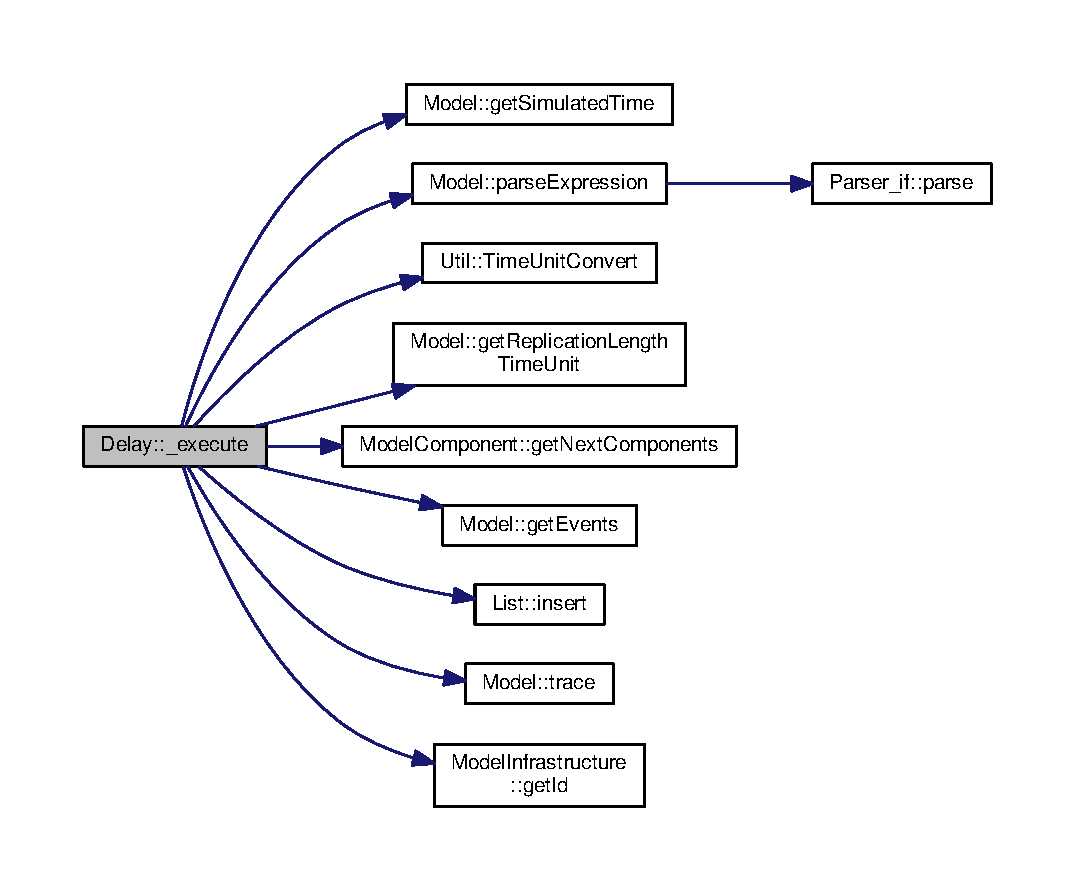
\includegraphics[width=350pt]{class_delay_a029d91a2cd736ff9c361c69336e6ab41_cgraph}
\end{center}
\end{figure}


\hypertarget{class_delay_a9d199bd226f9e504b6f6b6619d8f14dc}{\index{Delay@{Delay}!\-\_\-read\-Component@{\-\_\-read\-Component}}
\index{\-\_\-read\-Component@{\-\_\-read\-Component}!Delay@{Delay}}
\subsubsection[{\-\_\-read\-Component}]{\setlength{\rightskip}{0pt plus 5cm}void Delay\-::\-\_\-read\-Component (
\begin{DoxyParamCaption}
\item[{std\-::list$<$ std\-::string $>$}]{words}
\end{DoxyParamCaption}
)\hspace{0.3cm}{\ttfamily [protected]}, {\ttfamily [virtual]}}}\label{class_delay_a9d199bd226f9e504b6f6b6619d8f14dc}


Implements \hyperlink{class_model_component_aa16546b209d8fda2c8fa951e88652973}{Model\-Component}.

\hypertarget{class_delay_af1690df9ba58e9972f5721f5bdc2b520}{\index{Delay@{Delay}!\-\_\-verify\-Symbols@{\-\_\-verify\-Symbols}}
\index{\-\_\-verify\-Symbols@{\-\_\-verify\-Symbols}!Delay@{Delay}}
\subsubsection[{\-\_\-verify\-Symbols}]{\setlength{\rightskip}{0pt plus 5cm}bool Delay\-::\-\_\-verify\-Symbols (
\begin{DoxyParamCaption}
\item[{std\-::string $\ast$}]{error\-Message}
\end{DoxyParamCaption}
)\hspace{0.3cm}{\ttfamily [protected]}, {\ttfamily [virtual]}}}\label{class_delay_af1690df9ba58e9972f5721f5bdc2b520}


Implements \hyperlink{class_model_component_a183696468482133b2a09b761b7770521}{Model\-Component}.

\hypertarget{class_delay_aeb8506fddf709ad5e55fc67170e875b0}{\index{Delay@{Delay}!\-\_\-write\-Component@{\-\_\-write\-Component}}
\index{\-\_\-write\-Component@{\-\_\-write\-Component}!Delay@{Delay}}
\subsubsection[{\-\_\-write\-Component}]{\setlength{\rightskip}{0pt plus 5cm}std\-::list$<$ std\-::string $>$ $\ast$ Delay\-::\-\_\-write\-Component (
\begin{DoxyParamCaption}
{}
\end{DoxyParamCaption}
)\hspace{0.3cm}{\ttfamily [protected]}, {\ttfamily [virtual]}}}\label{class_delay_aeb8506fddf709ad5e55fc67170e875b0}


Implements \hyperlink{class_model_component_a5847971e860713d9df3e41c603c772c0}{Model\-Component}.

\hypertarget{class_delay_a58559eda9ed25330d29b967c1bb0add5}{\index{Delay@{Delay}!get\-Delay\-Expression@{get\-Delay\-Expression}}
\index{get\-Delay\-Expression@{get\-Delay\-Expression}!Delay@{Delay}}
\subsubsection[{get\-Delay\-Expression}]{\setlength{\rightskip}{0pt plus 5cm}std\-::string Delay\-::get\-Delay\-Expression (
\begin{DoxyParamCaption}
{}
\end{DoxyParamCaption}
) const}}\label{class_delay_a58559eda9ed25330d29b967c1bb0add5}
\hypertarget{class_delay_a0561a6fdb4dd317952b5bb8d87b0c15f}{\index{Delay@{Delay}!get\-Delay\-Time\-Unit@{get\-Delay\-Time\-Unit}}
\index{get\-Delay\-Time\-Unit@{get\-Delay\-Time\-Unit}!Delay@{Delay}}
\subsubsection[{get\-Delay\-Time\-Unit}]{\setlength{\rightskip}{0pt plus 5cm}{\bf Util\-::\-Time\-Unit} Delay\-::get\-Delay\-Time\-Unit (
\begin{DoxyParamCaption}
{}
\end{DoxyParamCaption}
) const}}\label{class_delay_a0561a6fdb4dd317952b5bb8d87b0c15f}
\hypertarget{class_delay_a683b53af607a424477acb946eb3afdfc}{\index{Delay@{Delay}!set\-Delay\-Expression@{set\-Delay\-Expression}}
\index{set\-Delay\-Expression@{set\-Delay\-Expression}!Delay@{Delay}}
\subsubsection[{set\-Delay\-Expression}]{\setlength{\rightskip}{0pt plus 5cm}void Delay\-::set\-Delay\-Expression (
\begin{DoxyParamCaption}
\item[{std\-::string}]{\-\_\-delay\-Expression}
\end{DoxyParamCaption}
)}}\label{class_delay_a683b53af607a424477acb946eb3afdfc}
\hypertarget{class_delay_abe7e89dba0974a81d00e6d2c0548fc1e}{\index{Delay@{Delay}!set\-Delay\-Time\-Unit@{set\-Delay\-Time\-Unit}}
\index{set\-Delay\-Time\-Unit@{set\-Delay\-Time\-Unit}!Delay@{Delay}}
\subsubsection[{set\-Delay\-Time\-Unit}]{\setlength{\rightskip}{0pt plus 5cm}void Delay\-::set\-Delay\-Time\-Unit (
\begin{DoxyParamCaption}
\item[{{\bf Util\-::\-Time\-Unit}}]{\-\_\-delay\-Time\-Unit}
\end{DoxyParamCaption}
)}}\label{class_delay_abe7e89dba0974a81d00e6d2c0548fc1e}
\hypertarget{class_delay_af8187e4515417b547dc22b5ee0a1f95d}{\index{Delay@{Delay}!show@{show}}
\index{show@{show}!Delay@{Delay}}
\subsubsection[{show}]{\setlength{\rightskip}{0pt plus 5cm}std\-::string Delay\-::show (
\begin{DoxyParamCaption}
{}
\end{DoxyParamCaption}
)\hspace{0.3cm}{\ttfamily [virtual]}}}\label{class_delay_af8187e4515417b547dc22b5ee0a1f95d}


Reimplemented from \hyperlink{class_model_component_ad8bc846e36b028eab7efb7da6c549eca}{Model\-Component}.



Here is the call graph for this function\-:\nopagebreak
\begin{figure}[H]
\begin{center}
\leavevmode
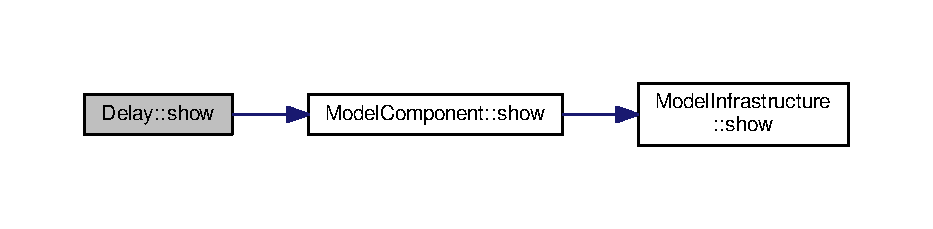
\includegraphics[width=350pt]{class_delay_af8187e4515417b547dc22b5ee0a1f95d_cgraph}
\end{center}
\end{figure}




The documentation for this class was generated from the following files\-:\begin{DoxyCompactItemize}
\item 
\hyperlink{_delay_8h}{Delay.\-h}\item 
\hyperlink{_delay_8cpp}{Delay.\-cpp}\end{DoxyCompactItemize}

\hypertarget{class_dispose}{\section{Dispose Class Reference}
\label{class_dispose}\index{Dispose@{Dispose}}
}


{\ttfamily \#include $<$Dispose.\-h$>$}



Inheritance diagram for Dispose\-:\nopagebreak
\begin{figure}[H]
\begin{center}
\leavevmode
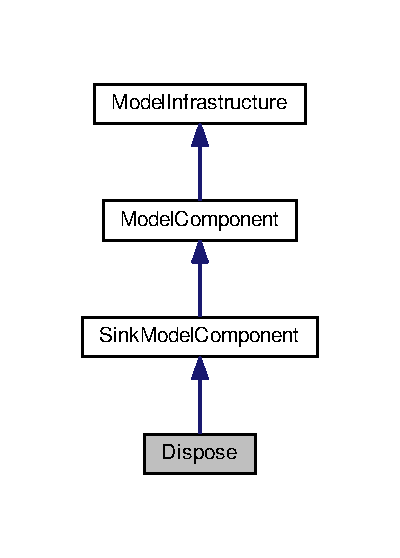
\includegraphics[width=192pt]{class_dispose__inherit__graph}
\end{center}
\end{figure}


Collaboration diagram for Dispose\-:\nopagebreak
\begin{figure}[H]
\begin{center}
\leavevmode
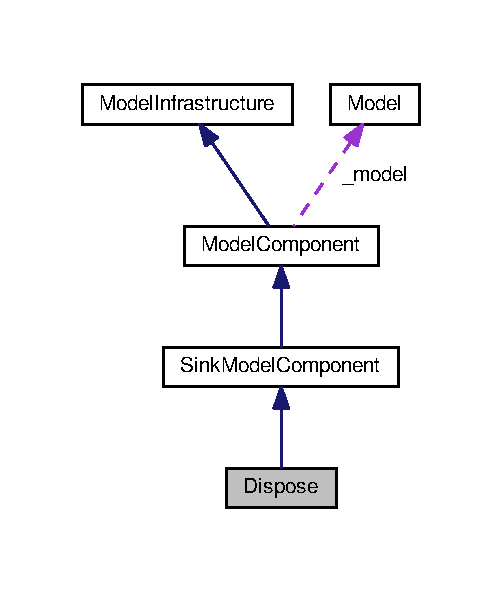
\includegraphics[width=241pt]{class_dispose__coll__graph}
\end{center}
\end{figure}
\subsection*{Public Member Functions}
\begin{DoxyCompactItemize}
\item 
\hyperlink{class_dispose_a9b5ccd61252e7f36d747fd832debdfaa}{Dispose} (\hyperlink{class_model}{Model} $\ast$model)
\item 
\hyperlink{class_dispose_a8d4515962baf1fd7c01912cb654aa683}{Dispose} (const \hyperlink{class_dispose}{Dispose} \&orig)
\item 
virtual \hyperlink{class_dispose_a2a2af23e9cbca66b02a142252a99096d}{$\sim$\-Dispose} ()
\item 
virtual std\-::string \hyperlink{class_dispose_aee8ef98d5ca22eb18a97b258ed059865}{show} ()
\item 
void \hyperlink{class_dispose_a8dc978664e640bc4d58760770b84b84e}{set\-Collect\-Statistics} (bool \-\_\-collect\-Statistics)
\item 
bool \hyperlink{class_dispose_aff15fbea8737b30efe9b3521d12350bd}{is\-Collect\-Statistics} () const 
\end{DoxyCompactItemize}
\subsection*{Protected Member Functions}
\begin{DoxyCompactItemize}
\item 
virtual void \hyperlink{class_dispose_a342eb428496534cdfd17524ad78b0c08}{\-\_\-execute} (\hyperlink{class_entity}{Entity} $\ast$entity)
\item 
virtual void \hyperlink{class_dispose_a2016b0e90d850753181417648557e3ce}{\-\_\-read\-Component} (std\-::list$<$ std\-::string $>$ words)
\item 
virtual std\-::list$<$ std\-::string $>$ $\ast$ \hyperlink{class_dispose_a2483f126094c4f58a2873ec7083a1903}{\-\_\-write\-Component} ()
\item 
virtual bool \hyperlink{class_dispose_a5ad64b97bbb16662aa9d914eda2a7e38}{\-\_\-verify\-Symbols} (std\-::string $\ast$error\-Message)
\end{DoxyCompactItemize}
\subsection*{Additional Inherited Members}


\subsection{Constructor \& Destructor Documentation}
\hypertarget{class_dispose_a9b5ccd61252e7f36d747fd832debdfaa}{\index{Dispose@{Dispose}!Dispose@{Dispose}}
\index{Dispose@{Dispose}!Dispose@{Dispose}}
\subsubsection[{Dispose}]{\setlength{\rightskip}{0pt plus 5cm}Dispose\-::\-Dispose (
\begin{DoxyParamCaption}
\item[{{\bf Model} $\ast$}]{model}
\end{DoxyParamCaption}
)}}\label{class_dispose_a9b5ccd61252e7f36d747fd832debdfaa}
\hypertarget{class_dispose_a8d4515962baf1fd7c01912cb654aa683}{\index{Dispose@{Dispose}!Dispose@{Dispose}}
\index{Dispose@{Dispose}!Dispose@{Dispose}}
\subsubsection[{Dispose}]{\setlength{\rightskip}{0pt plus 5cm}Dispose\-::\-Dispose (
\begin{DoxyParamCaption}
\item[{const {\bf Dispose} \&}]{orig}
\end{DoxyParamCaption}
)}}\label{class_dispose_a8d4515962baf1fd7c01912cb654aa683}
\hypertarget{class_dispose_a2a2af23e9cbca66b02a142252a99096d}{\index{Dispose@{Dispose}!$\sim$\-Dispose@{$\sim$\-Dispose}}
\index{$\sim$\-Dispose@{$\sim$\-Dispose}!Dispose@{Dispose}}
\subsubsection[{$\sim$\-Dispose}]{\setlength{\rightskip}{0pt plus 5cm}Dispose\-::$\sim$\-Dispose (
\begin{DoxyParamCaption}
{}
\end{DoxyParamCaption}
)\hspace{0.3cm}{\ttfamily [virtual]}}}\label{class_dispose_a2a2af23e9cbca66b02a142252a99096d}


\subsection{Member Function Documentation}
\hypertarget{class_dispose_a342eb428496534cdfd17524ad78b0c08}{\index{Dispose@{Dispose}!\-\_\-execute@{\-\_\-execute}}
\index{\-\_\-execute@{\-\_\-execute}!Dispose@{Dispose}}
\subsubsection[{\-\_\-execute}]{\setlength{\rightskip}{0pt plus 5cm}void Dispose\-::\-\_\-execute (
\begin{DoxyParamCaption}
\item[{{\bf Entity} $\ast$}]{entity}
\end{DoxyParamCaption}
)\hspace{0.3cm}{\ttfamily [protected]}, {\ttfamily [virtual]}}}\label{class_dispose_a342eb428496534cdfd17524ad78b0c08}


Implements \hyperlink{class_model_component_ae3fcf8bbdd8368c882438424aa73f714}{Model\-Component}.



Here is the call graph for this function\-:\nopagebreak
\begin{figure}[H]
\begin{center}
\leavevmode
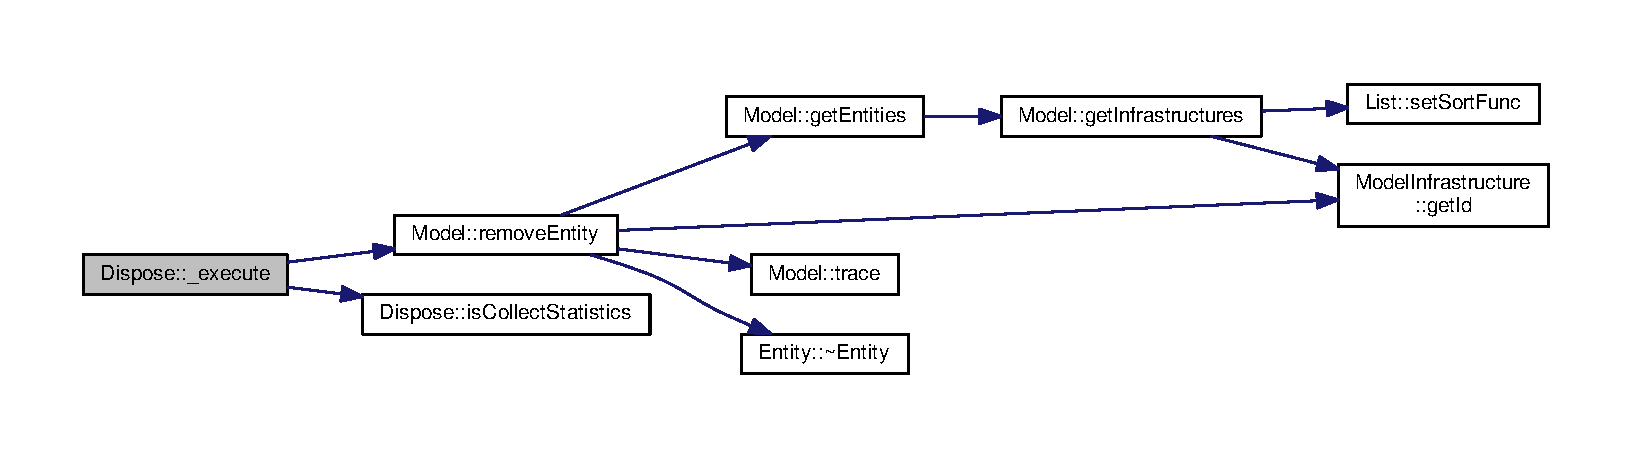
\includegraphics[width=350pt]{class_dispose_a342eb428496534cdfd17524ad78b0c08_cgraph}
\end{center}
\end{figure}


\hypertarget{class_dispose_a2016b0e90d850753181417648557e3ce}{\index{Dispose@{Dispose}!\-\_\-read\-Component@{\-\_\-read\-Component}}
\index{\-\_\-read\-Component@{\-\_\-read\-Component}!Dispose@{Dispose}}
\subsubsection[{\-\_\-read\-Component}]{\setlength{\rightskip}{0pt plus 5cm}void Dispose\-::\-\_\-read\-Component (
\begin{DoxyParamCaption}
\item[{std\-::list$<$ std\-::string $>$}]{words}
\end{DoxyParamCaption}
)\hspace{0.3cm}{\ttfamily [protected]}, {\ttfamily [virtual]}}}\label{class_dispose_a2016b0e90d850753181417648557e3ce}


Implements \hyperlink{class_model_component_aa16546b209d8fda2c8fa951e88652973}{Model\-Component}.

\hypertarget{class_dispose_a5ad64b97bbb16662aa9d914eda2a7e38}{\index{Dispose@{Dispose}!\-\_\-verify\-Symbols@{\-\_\-verify\-Symbols}}
\index{\-\_\-verify\-Symbols@{\-\_\-verify\-Symbols}!Dispose@{Dispose}}
\subsubsection[{\-\_\-verify\-Symbols}]{\setlength{\rightskip}{0pt plus 5cm}bool Dispose\-::\-\_\-verify\-Symbols (
\begin{DoxyParamCaption}
\item[{std\-::string $\ast$}]{error\-Message}
\end{DoxyParamCaption}
)\hspace{0.3cm}{\ttfamily [protected]}, {\ttfamily [virtual]}}}\label{class_dispose_a5ad64b97bbb16662aa9d914eda2a7e38}


Implements \hyperlink{class_model_component_a183696468482133b2a09b761b7770521}{Model\-Component}.

\hypertarget{class_dispose_a2483f126094c4f58a2873ec7083a1903}{\index{Dispose@{Dispose}!\-\_\-write\-Component@{\-\_\-write\-Component}}
\index{\-\_\-write\-Component@{\-\_\-write\-Component}!Dispose@{Dispose}}
\subsubsection[{\-\_\-write\-Component}]{\setlength{\rightskip}{0pt plus 5cm}std\-::list$<$ std\-::string $>$ $\ast$ Dispose\-::\-\_\-write\-Component (
\begin{DoxyParamCaption}
{}
\end{DoxyParamCaption}
)\hspace{0.3cm}{\ttfamily [protected]}, {\ttfamily [virtual]}}}\label{class_dispose_a2483f126094c4f58a2873ec7083a1903}


Implements \hyperlink{class_model_component_a5847971e860713d9df3e41c603c772c0}{Model\-Component}.

\hypertarget{class_dispose_aff15fbea8737b30efe9b3521d12350bd}{\index{Dispose@{Dispose}!is\-Collect\-Statistics@{is\-Collect\-Statistics}}
\index{is\-Collect\-Statistics@{is\-Collect\-Statistics}!Dispose@{Dispose}}
\subsubsection[{is\-Collect\-Statistics}]{\setlength{\rightskip}{0pt plus 5cm}bool Dispose\-::is\-Collect\-Statistics (
\begin{DoxyParamCaption}
{}
\end{DoxyParamCaption}
) const}}\label{class_dispose_aff15fbea8737b30efe9b3521d12350bd}
\hypertarget{class_dispose_a8dc978664e640bc4d58760770b84b84e}{\index{Dispose@{Dispose}!set\-Collect\-Statistics@{set\-Collect\-Statistics}}
\index{set\-Collect\-Statistics@{set\-Collect\-Statistics}!Dispose@{Dispose}}
\subsubsection[{set\-Collect\-Statistics}]{\setlength{\rightskip}{0pt plus 5cm}void Dispose\-::set\-Collect\-Statistics (
\begin{DoxyParamCaption}
\item[{bool}]{\-\_\-collect\-Statistics}
\end{DoxyParamCaption}
)}}\label{class_dispose_a8dc978664e640bc4d58760770b84b84e}
\hypertarget{class_dispose_aee8ef98d5ca22eb18a97b258ed059865}{\index{Dispose@{Dispose}!show@{show}}
\index{show@{show}!Dispose@{Dispose}}
\subsubsection[{show}]{\setlength{\rightskip}{0pt plus 5cm}std\-::string Dispose\-::show (
\begin{DoxyParamCaption}
{}
\end{DoxyParamCaption}
)\hspace{0.3cm}{\ttfamily [virtual]}}}\label{class_dispose_aee8ef98d5ca22eb18a97b258ed059865}


Reimplemented from \hyperlink{class_model_component_ad8bc846e36b028eab7efb7da6c549eca}{Model\-Component}.



Here is the call graph for this function\-:\nopagebreak
\begin{figure}[H]
\begin{center}
\leavevmode
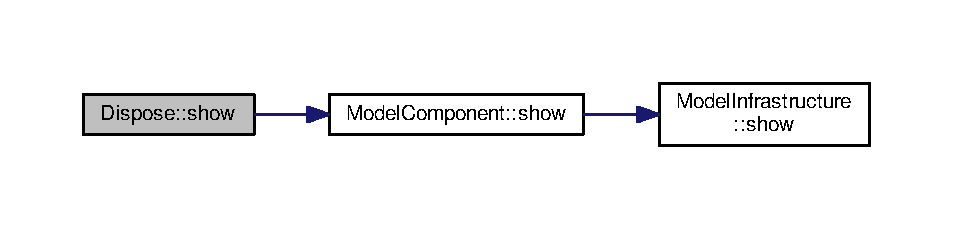
\includegraphics[width=350pt]{class_dispose_aee8ef98d5ca22eb18a97b258ed059865_cgraph}
\end{center}
\end{figure}




The documentation for this class was generated from the following files\-:\begin{DoxyCompactItemize}
\item 
\hyperlink{_dispose_8h}{Dispose.\-h}\item 
\hyperlink{_dispose_8cpp}{Dispose.\-cpp}\end{DoxyCompactItemize}

\hypertarget{class_entity}{\section{Entity Class Reference}
\label{class_entity}\index{Entity@{Entity}}
}


{\ttfamily \#include $<$Entity.\-h$>$}



Inheritance diagram for Entity\-:\nopagebreak
\begin{figure}[H]
\begin{center}
\leavevmode
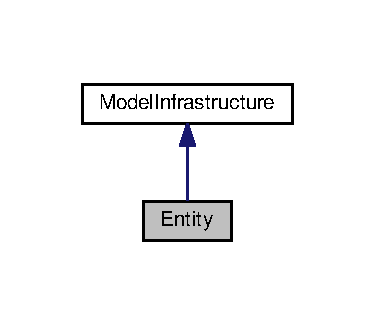
\includegraphics[width=180pt]{class_entity__inherit__graph}
\end{center}
\end{figure}


Collaboration diagram for Entity\-:\nopagebreak
\begin{figure}[H]
\begin{center}
\leavevmode
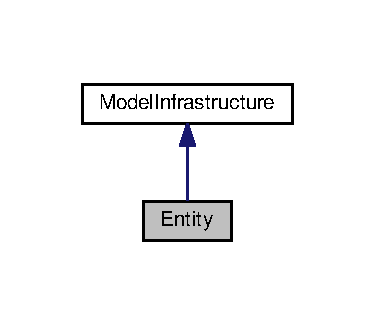
\includegraphics[width=180pt]{class_entity__coll__graph}
\end{center}
\end{figure}
\subsection*{Public Member Functions}
\begin{DoxyCompactItemize}
\item 
\hyperlink{class_entity_a980f368aa07ce358583982821533a54a}{Entity} ()
\item 
\hyperlink{class_entity_a9de139ff12775dd95fb80bec08247de7}{Entity} (const \hyperlink{class_entity}{Entity} \&orig)
\item 
virtual \hyperlink{class_entity_adf6d3f7cb1b2ba029b6b048a395cc8ae}{$\sim$\-Entity} ()
\item 
virtual std\-::string \hyperlink{class_entity_a86cc324050b451b31b134943e7978e36}{show} ()
\item 
std\-::map$<$ std\-::string, \\*
\hyperlink{class_attribute_value}{Attribute\-Value} $\ast$ $>$ $\ast$ \hyperlink{class_entity_a5990dbefc2f21a7e8e0f91f9bf434fb9}{get\-Attribute\-Values} () const 
\item 
void \hyperlink{class_entity_a40053760a2c84dd72fd5aeb425f6781d}{set\-Entity\-Type\-Name} (std\-::string \-\_\-entity\-Type\-Name)
\item 
std\-::string \hyperlink{class_entity_a860a6385aa2af6b8d205a8e3ea912c38}{get\-Entity\-Type\-Name} () const 
\end{DoxyCompactItemize}
\subsection*{Additional Inherited Members}


\subsection{Constructor \& Destructor Documentation}
\hypertarget{class_entity_a980f368aa07ce358583982821533a54a}{\index{Entity@{Entity}!Entity@{Entity}}
\index{Entity@{Entity}!Entity@{Entity}}
\subsubsection[{Entity}]{\setlength{\rightskip}{0pt plus 5cm}Entity\-::\-Entity (
\begin{DoxyParamCaption}
{}
\end{DoxyParamCaption}
)}}\label{class_entity_a980f368aa07ce358583982821533a54a}
\hypertarget{class_entity_a9de139ff12775dd95fb80bec08247de7}{\index{Entity@{Entity}!Entity@{Entity}}
\index{Entity@{Entity}!Entity@{Entity}}
\subsubsection[{Entity}]{\setlength{\rightskip}{0pt plus 5cm}Entity\-::\-Entity (
\begin{DoxyParamCaption}
\item[{const {\bf Entity} \&}]{orig}
\end{DoxyParamCaption}
)}}\label{class_entity_a9de139ff12775dd95fb80bec08247de7}
\hypertarget{class_entity_adf6d3f7cb1b2ba029b6b048a395cc8ae}{\index{Entity@{Entity}!$\sim$\-Entity@{$\sim$\-Entity}}
\index{$\sim$\-Entity@{$\sim$\-Entity}!Entity@{Entity}}
\subsubsection[{$\sim$\-Entity}]{\setlength{\rightskip}{0pt plus 5cm}Entity\-::$\sim$\-Entity (
\begin{DoxyParamCaption}
{}
\end{DoxyParamCaption}
)\hspace{0.3cm}{\ttfamily [virtual]}}}\label{class_entity_adf6d3f7cb1b2ba029b6b048a395cc8ae}


\subsection{Member Function Documentation}
\hypertarget{class_entity_a5990dbefc2f21a7e8e0f91f9bf434fb9}{\index{Entity@{Entity}!get\-Attribute\-Values@{get\-Attribute\-Values}}
\index{get\-Attribute\-Values@{get\-Attribute\-Values}!Entity@{Entity}}
\subsubsection[{get\-Attribute\-Values}]{\setlength{\rightskip}{0pt plus 5cm}std\-::map$<$ std\-::string, {\bf Attribute\-Value} $\ast$ $>$ $\ast$ Entity\-::get\-Attribute\-Values (
\begin{DoxyParamCaption}
{}
\end{DoxyParamCaption}
) const}}\label{class_entity_a5990dbefc2f21a7e8e0f91f9bf434fb9}
\hypertarget{class_entity_a860a6385aa2af6b8d205a8e3ea912c38}{\index{Entity@{Entity}!get\-Entity\-Type\-Name@{get\-Entity\-Type\-Name}}
\index{get\-Entity\-Type\-Name@{get\-Entity\-Type\-Name}!Entity@{Entity}}
\subsubsection[{get\-Entity\-Type\-Name}]{\setlength{\rightskip}{0pt plus 5cm}std\-::string Entity\-::get\-Entity\-Type\-Name (
\begin{DoxyParamCaption}
{}
\end{DoxyParamCaption}
) const}}\label{class_entity_a860a6385aa2af6b8d205a8e3ea912c38}
\hypertarget{class_entity_a40053760a2c84dd72fd5aeb425f6781d}{\index{Entity@{Entity}!set\-Entity\-Type\-Name@{set\-Entity\-Type\-Name}}
\index{set\-Entity\-Type\-Name@{set\-Entity\-Type\-Name}!Entity@{Entity}}
\subsubsection[{set\-Entity\-Type\-Name}]{\setlength{\rightskip}{0pt plus 5cm}void Entity\-::set\-Entity\-Type\-Name (
\begin{DoxyParamCaption}
\item[{std\-::string}]{\-\_\-entity\-Type\-Name}
\end{DoxyParamCaption}
)}}\label{class_entity_a40053760a2c84dd72fd5aeb425f6781d}
\hypertarget{class_entity_a86cc324050b451b31b134943e7978e36}{\index{Entity@{Entity}!show@{show}}
\index{show@{show}!Entity@{Entity}}
\subsubsection[{show}]{\setlength{\rightskip}{0pt plus 5cm}std\-::string Entity\-::show (
\begin{DoxyParamCaption}
{}
\end{DoxyParamCaption}
)\hspace{0.3cm}{\ttfamily [virtual]}}}\label{class_entity_a86cc324050b451b31b134943e7978e36}


Reimplemented from \hyperlink{class_model_infrastructure_a649a5a89a0c9931783d3c51de2acf266}{Model\-Infrastructure}.



Here is the call graph for this function\-:\nopagebreak
\begin{figure}[H]
\begin{center}
\leavevmode
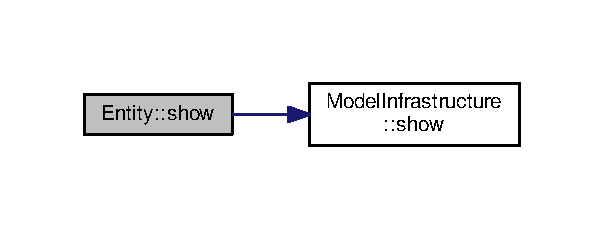
\includegraphics[width=290pt]{class_entity_a86cc324050b451b31b134943e7978e36_cgraph}
\end{center}
\end{figure}




The documentation for this class was generated from the following files\-:\begin{DoxyCompactItemize}
\item 
\hyperlink{_entity_8h}{Entity.\-h}\item 
\hyperlink{_entity_8cpp}{Entity.\-cpp}\end{DoxyCompactItemize}

\hypertarget{class_entity_type}{\section{Entity\-Type Class Reference}
\label{class_entity_type}\index{Entity\-Type@{Entity\-Type}}
}


{\ttfamily \#include $<$Entity\-Type.\-h$>$}



Inheritance diagram for Entity\-Type\-:\nopagebreak
\begin{figure}[H]
\begin{center}
\leavevmode
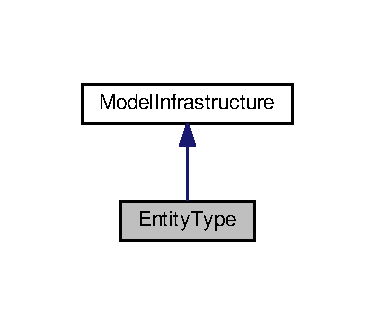
\includegraphics[width=180pt]{class_entity_type__inherit__graph}
\end{center}
\end{figure}


Collaboration diagram for Entity\-Type\-:\nopagebreak
\begin{figure}[H]
\begin{center}
\leavevmode
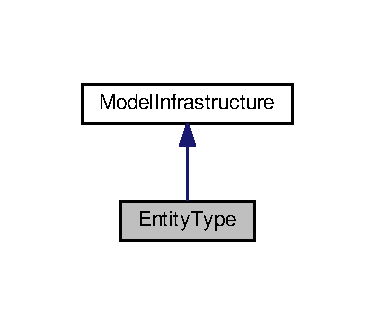
\includegraphics[width=180pt]{class_entity_type__coll__graph}
\end{center}
\end{figure}
\subsection*{Public Member Functions}
\begin{DoxyCompactItemize}
\item 
\hyperlink{class_entity_type_abea5cf6495bb0fb677ccf0a5e52716d3}{Entity\-Type} ()
\item 
\hyperlink{class_entity_type_a34b9576e2453ed309c75840319bbb2f8}{Entity\-Type} (const \hyperlink{class_entity_type}{Entity\-Type} \&orig)
\item 
virtual \hyperlink{class_entity_type_aee11e4242d000965f06018723bdf0946}{$\sim$\-Entity\-Type} ()
\item 
virtual std\-::string \hyperlink{class_entity_type_ab5a696912b12a9f51decded90f368dea}{show} ()
\item 
void \hyperlink{class_entity_type_affd1d2dd13149ae0989aae5cc9ea1e05}{set\-Initial\-Waiting\-Cost} (double \-\_\-initial\-Waiting\-Cost)
\item 
double \hyperlink{class_entity_type_a46dd0977b19bf167eeb12db97464b757}{get\-Initial\-Waiting\-Cost} () const 
\item 
void \hyperlink{class_entity_type_a32f126822c567a887a446a763db13d64}{set\-Initial\-Other\-Cost} (double \-\_\-initial\-Other\-Cost)
\item 
double \hyperlink{class_entity_type_ac5708811f5f6eaf7ac587fc88190b7f2}{get\-Initial\-Other\-Cost} () const 
\item 
void \hyperlink{class_entity_type_a935cac67adc2b13aa25290c3db04c847}{set\-Initial\-N\-V\-A\-Cost} (double \-\_\-initial\-N\-V\-A\-Cost)
\item 
double \hyperlink{class_entity_type_ae8b26deba82e687d5a07b863f750baf4}{get\-Initial\-N\-V\-A\-Cost} () const 
\item 
void \hyperlink{class_entity_type_aecd52de7178bb03be55798378d15d3e8}{set\-Initial\-V\-A\-Cost} (double \-\_\-initial\-V\-A\-Cost)
\item 
double \hyperlink{class_entity_type_a9833d4a85dcb5c5bd9db02e1e2e45dd9}{get\-Initial\-V\-A\-Cost} () const 
\item 
void \hyperlink{class_entity_type_ab3a19031f9b46b376bdd35aa3044c90e}{set\-Initial\-Picture} (std\-::string \-\_\-initial\-Picture)
\item 
std\-::string \hyperlink{class_entity_type_a9a464c546bc2f7fe56fbea9b761ac1f7}{get\-Initial\-Picture} () const 
\item 
\hyperlink{class_collector__if}{Collector\-\_\-if} $\ast$ \hyperlink{class_entity_type_a03977d36fb845ba7366185fa1f5fffd9}{get\-Cstat\-Time\-In\-System} () const 
\item 
\hyperlink{class_collector__if}{Collector\-\_\-if} $\ast$ \hyperlink{class_entity_type_acf55bd71e2f6bb30ea6a01a98afe7422}{get\-Cstat\-N\-V\-A\-Time} () const 
\item 
\hyperlink{class_collector__if}{Collector\-\_\-if} $\ast$ \hyperlink{class_entity_type_a846625383404c36329af057f674d825c}{get\-Cstat\-V\-A\-Time} () const 
\item 
\hyperlink{class_collector__if}{Collector\-\_\-if} $\ast$ \hyperlink{class_entity_type_abe5f66a11ccc80a4138b1f44c1e8a9fe}{get\-Cstat\-Other\-Time} () const 
\item 
\hyperlink{class_collector__if}{Collector\-\_\-if} $\ast$ \hyperlink{class_entity_type_acc36d61158eb2f6ab72caca114023bc2}{get\-Cstat\-Transfer\-Time} () const 
\item 
\hyperlink{class_collector__if}{Collector\-\_\-if} $\ast$ \hyperlink{class_entity_type_ac2682128310221efaaa81b3007ef8d50}{get\-Cstat\-Waiting\-Time} () const 
\end{DoxyCompactItemize}
\subsection*{Additional Inherited Members}


\subsection{Constructor \& Destructor Documentation}
\hypertarget{class_entity_type_abea5cf6495bb0fb677ccf0a5e52716d3}{\index{Entity\-Type@{Entity\-Type}!Entity\-Type@{Entity\-Type}}
\index{Entity\-Type@{Entity\-Type}!EntityType@{Entity\-Type}}
\subsubsection[{Entity\-Type}]{\setlength{\rightskip}{0pt plus 5cm}Entity\-Type\-::\-Entity\-Type (
\begin{DoxyParamCaption}
{}
\end{DoxyParamCaption}
)}}\label{class_entity_type_abea5cf6495bb0fb677ccf0a5e52716d3}
\hypertarget{class_entity_type_a34b9576e2453ed309c75840319bbb2f8}{\index{Entity\-Type@{Entity\-Type}!Entity\-Type@{Entity\-Type}}
\index{Entity\-Type@{Entity\-Type}!EntityType@{Entity\-Type}}
\subsubsection[{Entity\-Type}]{\setlength{\rightskip}{0pt plus 5cm}Entity\-Type\-::\-Entity\-Type (
\begin{DoxyParamCaption}
\item[{const {\bf Entity\-Type} \&}]{orig}
\end{DoxyParamCaption}
)}}\label{class_entity_type_a34b9576e2453ed309c75840319bbb2f8}
\hypertarget{class_entity_type_aee11e4242d000965f06018723bdf0946}{\index{Entity\-Type@{Entity\-Type}!$\sim$\-Entity\-Type@{$\sim$\-Entity\-Type}}
\index{$\sim$\-Entity\-Type@{$\sim$\-Entity\-Type}!EntityType@{Entity\-Type}}
\subsubsection[{$\sim$\-Entity\-Type}]{\setlength{\rightskip}{0pt plus 5cm}Entity\-Type\-::$\sim$\-Entity\-Type (
\begin{DoxyParamCaption}
{}
\end{DoxyParamCaption}
)\hspace{0.3cm}{\ttfamily [virtual]}}}\label{class_entity_type_aee11e4242d000965f06018723bdf0946}


\subsection{Member Function Documentation}
\hypertarget{class_entity_type_acf55bd71e2f6bb30ea6a01a98afe7422}{\index{Entity\-Type@{Entity\-Type}!get\-Cstat\-N\-V\-A\-Time@{get\-Cstat\-N\-V\-A\-Time}}
\index{get\-Cstat\-N\-V\-A\-Time@{get\-Cstat\-N\-V\-A\-Time}!EntityType@{Entity\-Type}}
\subsubsection[{get\-Cstat\-N\-V\-A\-Time}]{\setlength{\rightskip}{0pt plus 5cm}{\bf Collector\-\_\-if} $\ast$ Entity\-Type\-::get\-Cstat\-N\-V\-A\-Time (
\begin{DoxyParamCaption}
{}
\end{DoxyParamCaption}
) const}}\label{class_entity_type_acf55bd71e2f6bb30ea6a01a98afe7422}
\hypertarget{class_entity_type_abe5f66a11ccc80a4138b1f44c1e8a9fe}{\index{Entity\-Type@{Entity\-Type}!get\-Cstat\-Other\-Time@{get\-Cstat\-Other\-Time}}
\index{get\-Cstat\-Other\-Time@{get\-Cstat\-Other\-Time}!EntityType@{Entity\-Type}}
\subsubsection[{get\-Cstat\-Other\-Time}]{\setlength{\rightskip}{0pt plus 5cm}{\bf Collector\-\_\-if} $\ast$ Entity\-Type\-::get\-Cstat\-Other\-Time (
\begin{DoxyParamCaption}
{}
\end{DoxyParamCaption}
) const}}\label{class_entity_type_abe5f66a11ccc80a4138b1f44c1e8a9fe}
\hypertarget{class_entity_type_a03977d36fb845ba7366185fa1f5fffd9}{\index{Entity\-Type@{Entity\-Type}!get\-Cstat\-Time\-In\-System@{get\-Cstat\-Time\-In\-System}}
\index{get\-Cstat\-Time\-In\-System@{get\-Cstat\-Time\-In\-System}!EntityType@{Entity\-Type}}
\subsubsection[{get\-Cstat\-Time\-In\-System}]{\setlength{\rightskip}{0pt plus 5cm}{\bf Collector\-\_\-if} $\ast$ Entity\-Type\-::get\-Cstat\-Time\-In\-System (
\begin{DoxyParamCaption}
{}
\end{DoxyParamCaption}
) const}}\label{class_entity_type_a03977d36fb845ba7366185fa1f5fffd9}
\hypertarget{class_entity_type_acc36d61158eb2f6ab72caca114023bc2}{\index{Entity\-Type@{Entity\-Type}!get\-Cstat\-Transfer\-Time@{get\-Cstat\-Transfer\-Time}}
\index{get\-Cstat\-Transfer\-Time@{get\-Cstat\-Transfer\-Time}!EntityType@{Entity\-Type}}
\subsubsection[{get\-Cstat\-Transfer\-Time}]{\setlength{\rightskip}{0pt plus 5cm}{\bf Collector\-\_\-if} $\ast$ Entity\-Type\-::get\-Cstat\-Transfer\-Time (
\begin{DoxyParamCaption}
{}
\end{DoxyParamCaption}
) const}}\label{class_entity_type_acc36d61158eb2f6ab72caca114023bc2}
\hypertarget{class_entity_type_a846625383404c36329af057f674d825c}{\index{Entity\-Type@{Entity\-Type}!get\-Cstat\-V\-A\-Time@{get\-Cstat\-V\-A\-Time}}
\index{get\-Cstat\-V\-A\-Time@{get\-Cstat\-V\-A\-Time}!EntityType@{Entity\-Type}}
\subsubsection[{get\-Cstat\-V\-A\-Time}]{\setlength{\rightskip}{0pt plus 5cm}{\bf Collector\-\_\-if} $\ast$ Entity\-Type\-::get\-Cstat\-V\-A\-Time (
\begin{DoxyParamCaption}
{}
\end{DoxyParamCaption}
) const}}\label{class_entity_type_a846625383404c36329af057f674d825c}
\hypertarget{class_entity_type_ac2682128310221efaaa81b3007ef8d50}{\index{Entity\-Type@{Entity\-Type}!get\-Cstat\-Waiting\-Time@{get\-Cstat\-Waiting\-Time}}
\index{get\-Cstat\-Waiting\-Time@{get\-Cstat\-Waiting\-Time}!EntityType@{Entity\-Type}}
\subsubsection[{get\-Cstat\-Waiting\-Time}]{\setlength{\rightskip}{0pt plus 5cm}{\bf Collector\-\_\-if} $\ast$ Entity\-Type\-::get\-Cstat\-Waiting\-Time (
\begin{DoxyParamCaption}
{}
\end{DoxyParamCaption}
) const}}\label{class_entity_type_ac2682128310221efaaa81b3007ef8d50}
\hypertarget{class_entity_type_ae8b26deba82e687d5a07b863f750baf4}{\index{Entity\-Type@{Entity\-Type}!get\-Initial\-N\-V\-A\-Cost@{get\-Initial\-N\-V\-A\-Cost}}
\index{get\-Initial\-N\-V\-A\-Cost@{get\-Initial\-N\-V\-A\-Cost}!EntityType@{Entity\-Type}}
\subsubsection[{get\-Initial\-N\-V\-A\-Cost}]{\setlength{\rightskip}{0pt plus 5cm}double Entity\-Type\-::get\-Initial\-N\-V\-A\-Cost (
\begin{DoxyParamCaption}
{}
\end{DoxyParamCaption}
) const}}\label{class_entity_type_ae8b26deba82e687d5a07b863f750baf4}
\hypertarget{class_entity_type_ac5708811f5f6eaf7ac587fc88190b7f2}{\index{Entity\-Type@{Entity\-Type}!get\-Initial\-Other\-Cost@{get\-Initial\-Other\-Cost}}
\index{get\-Initial\-Other\-Cost@{get\-Initial\-Other\-Cost}!EntityType@{Entity\-Type}}
\subsubsection[{get\-Initial\-Other\-Cost}]{\setlength{\rightskip}{0pt plus 5cm}double Entity\-Type\-::get\-Initial\-Other\-Cost (
\begin{DoxyParamCaption}
{}
\end{DoxyParamCaption}
) const}}\label{class_entity_type_ac5708811f5f6eaf7ac587fc88190b7f2}
\hypertarget{class_entity_type_a9a464c546bc2f7fe56fbea9b761ac1f7}{\index{Entity\-Type@{Entity\-Type}!get\-Initial\-Picture@{get\-Initial\-Picture}}
\index{get\-Initial\-Picture@{get\-Initial\-Picture}!EntityType@{Entity\-Type}}
\subsubsection[{get\-Initial\-Picture}]{\setlength{\rightskip}{0pt plus 5cm}std\-::string Entity\-Type\-::get\-Initial\-Picture (
\begin{DoxyParamCaption}
{}
\end{DoxyParamCaption}
) const}}\label{class_entity_type_a9a464c546bc2f7fe56fbea9b761ac1f7}
\hypertarget{class_entity_type_a9833d4a85dcb5c5bd9db02e1e2e45dd9}{\index{Entity\-Type@{Entity\-Type}!get\-Initial\-V\-A\-Cost@{get\-Initial\-V\-A\-Cost}}
\index{get\-Initial\-V\-A\-Cost@{get\-Initial\-V\-A\-Cost}!EntityType@{Entity\-Type}}
\subsubsection[{get\-Initial\-V\-A\-Cost}]{\setlength{\rightskip}{0pt plus 5cm}double Entity\-Type\-::get\-Initial\-V\-A\-Cost (
\begin{DoxyParamCaption}
{}
\end{DoxyParamCaption}
) const}}\label{class_entity_type_a9833d4a85dcb5c5bd9db02e1e2e45dd9}
\hypertarget{class_entity_type_a46dd0977b19bf167eeb12db97464b757}{\index{Entity\-Type@{Entity\-Type}!get\-Initial\-Waiting\-Cost@{get\-Initial\-Waiting\-Cost}}
\index{get\-Initial\-Waiting\-Cost@{get\-Initial\-Waiting\-Cost}!EntityType@{Entity\-Type}}
\subsubsection[{get\-Initial\-Waiting\-Cost}]{\setlength{\rightskip}{0pt plus 5cm}double Entity\-Type\-::get\-Initial\-Waiting\-Cost (
\begin{DoxyParamCaption}
{}
\end{DoxyParamCaption}
) const}}\label{class_entity_type_a46dd0977b19bf167eeb12db97464b757}
\hypertarget{class_entity_type_a935cac67adc2b13aa25290c3db04c847}{\index{Entity\-Type@{Entity\-Type}!set\-Initial\-N\-V\-A\-Cost@{set\-Initial\-N\-V\-A\-Cost}}
\index{set\-Initial\-N\-V\-A\-Cost@{set\-Initial\-N\-V\-A\-Cost}!EntityType@{Entity\-Type}}
\subsubsection[{set\-Initial\-N\-V\-A\-Cost}]{\setlength{\rightskip}{0pt plus 5cm}void Entity\-Type\-::set\-Initial\-N\-V\-A\-Cost (
\begin{DoxyParamCaption}
\item[{double}]{\-\_\-initial\-N\-V\-A\-Cost}
\end{DoxyParamCaption}
)}}\label{class_entity_type_a935cac67adc2b13aa25290c3db04c847}
\hypertarget{class_entity_type_a32f126822c567a887a446a763db13d64}{\index{Entity\-Type@{Entity\-Type}!set\-Initial\-Other\-Cost@{set\-Initial\-Other\-Cost}}
\index{set\-Initial\-Other\-Cost@{set\-Initial\-Other\-Cost}!EntityType@{Entity\-Type}}
\subsubsection[{set\-Initial\-Other\-Cost}]{\setlength{\rightskip}{0pt plus 5cm}void Entity\-Type\-::set\-Initial\-Other\-Cost (
\begin{DoxyParamCaption}
\item[{double}]{\-\_\-initial\-Other\-Cost}
\end{DoxyParamCaption}
)}}\label{class_entity_type_a32f126822c567a887a446a763db13d64}
\hypertarget{class_entity_type_ab3a19031f9b46b376bdd35aa3044c90e}{\index{Entity\-Type@{Entity\-Type}!set\-Initial\-Picture@{set\-Initial\-Picture}}
\index{set\-Initial\-Picture@{set\-Initial\-Picture}!EntityType@{Entity\-Type}}
\subsubsection[{set\-Initial\-Picture}]{\setlength{\rightskip}{0pt plus 5cm}void Entity\-Type\-::set\-Initial\-Picture (
\begin{DoxyParamCaption}
\item[{std\-::string}]{\-\_\-initial\-Picture}
\end{DoxyParamCaption}
)}}\label{class_entity_type_ab3a19031f9b46b376bdd35aa3044c90e}
\hypertarget{class_entity_type_aecd52de7178bb03be55798378d15d3e8}{\index{Entity\-Type@{Entity\-Type}!set\-Initial\-V\-A\-Cost@{set\-Initial\-V\-A\-Cost}}
\index{set\-Initial\-V\-A\-Cost@{set\-Initial\-V\-A\-Cost}!EntityType@{Entity\-Type}}
\subsubsection[{set\-Initial\-V\-A\-Cost}]{\setlength{\rightskip}{0pt plus 5cm}void Entity\-Type\-::set\-Initial\-V\-A\-Cost (
\begin{DoxyParamCaption}
\item[{double}]{\-\_\-initial\-V\-A\-Cost}
\end{DoxyParamCaption}
)}}\label{class_entity_type_aecd52de7178bb03be55798378d15d3e8}
\hypertarget{class_entity_type_affd1d2dd13149ae0989aae5cc9ea1e05}{\index{Entity\-Type@{Entity\-Type}!set\-Initial\-Waiting\-Cost@{set\-Initial\-Waiting\-Cost}}
\index{set\-Initial\-Waiting\-Cost@{set\-Initial\-Waiting\-Cost}!EntityType@{Entity\-Type}}
\subsubsection[{set\-Initial\-Waiting\-Cost}]{\setlength{\rightskip}{0pt plus 5cm}void Entity\-Type\-::set\-Initial\-Waiting\-Cost (
\begin{DoxyParamCaption}
\item[{double}]{\-\_\-initial\-Waiting\-Cost}
\end{DoxyParamCaption}
)}}\label{class_entity_type_affd1d2dd13149ae0989aae5cc9ea1e05}
\hypertarget{class_entity_type_ab5a696912b12a9f51decded90f368dea}{\index{Entity\-Type@{Entity\-Type}!show@{show}}
\index{show@{show}!EntityType@{Entity\-Type}}
\subsubsection[{show}]{\setlength{\rightskip}{0pt plus 5cm}std\-::string Entity\-Type\-::show (
\begin{DoxyParamCaption}
{}
\end{DoxyParamCaption}
)\hspace{0.3cm}{\ttfamily [virtual]}}}\label{class_entity_type_ab5a696912b12a9f51decded90f368dea}


Reimplemented from \hyperlink{class_model_infrastructure_a649a5a89a0c9931783d3c51de2acf266}{Model\-Infrastructure}.



Here is the call graph for this function\-:\nopagebreak
\begin{figure}[H]
\begin{center}
\leavevmode
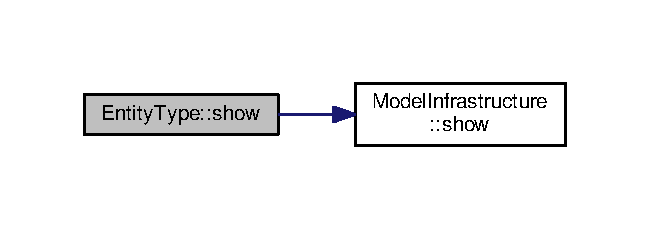
\includegraphics[width=312pt]{class_entity_type_ab5a696912b12a9f51decded90f368dea_cgraph}
\end{center}
\end{figure}




The documentation for this class was generated from the following files\-:\begin{DoxyCompactItemize}
\item 
\hyperlink{_entity_type_8h}{Entity\-Type.\-h}\item 
\hyperlink{_entity_type_8cpp}{Entity\-Type.\-cpp}\end{DoxyCompactItemize}

\hypertarget{class_event}{\section{Event Class Reference}
\label{class_event}\index{Event@{Event}}
}


{\ttfamily \#include $<$Event.\-h$>$}

\subsection*{Public Member Functions}
\begin{DoxyCompactItemize}
\item 
\hyperlink{class_event_a81e573f9452ca3a4d1b07e2347235e87}{Event} (double time, \hyperlink{class_entity}{Entity} $\ast$entity, \hyperlink{class_model_component}{Model\-Component} $\ast$component)
\item 
\hyperlink{class_event_a537ad58d679329069468e8cf2b2904d0}{Event} (const \hyperlink{class_event}{Event} \&orig)
\item 
virtual \hyperlink{class_event_a7704ec01ce91e673885792054214b3d2}{$\sim$\-Event} ()
\item 
double \hyperlink{class_event_a008a7989d0849a45613917cedc27f27e}{get\-Time} () const 
\item 
\hyperlink{class_model_component}{Model\-Component} $\ast$ \hyperlink{class_event_a7fb897ded1b3f0b946b25740f2e2eda0}{get\-Component} () const 
\item 
\hyperlink{class_entity}{Entity} $\ast$ \hyperlink{class_event_a6890c776c6c2e13abbc0892fc7333102}{get\-Entity} () const 
\item 
std\-::string \hyperlink{class_event_a640f132001d454af52cb0d0e20ebb856}{show} ()
\end{DoxyCompactItemize}


\subsection{Constructor \& Destructor Documentation}
\hypertarget{class_event_a81e573f9452ca3a4d1b07e2347235e87}{\index{Event@{Event}!Event@{Event}}
\index{Event@{Event}!Event@{Event}}
\subsubsection[{Event}]{\setlength{\rightskip}{0pt plus 5cm}Event\-::\-Event (
\begin{DoxyParamCaption}
\item[{double}]{time, }
\item[{{\bf Entity} $\ast$}]{entity, }
\item[{{\bf Model\-Component} $\ast$}]{component}
\end{DoxyParamCaption}
)}}\label{class_event_a81e573f9452ca3a4d1b07e2347235e87}
\hypertarget{class_event_a537ad58d679329069468e8cf2b2904d0}{\index{Event@{Event}!Event@{Event}}
\index{Event@{Event}!Event@{Event}}
\subsubsection[{Event}]{\setlength{\rightskip}{0pt plus 5cm}Event\-::\-Event (
\begin{DoxyParamCaption}
\item[{const {\bf Event} \&}]{orig}
\end{DoxyParamCaption}
)}}\label{class_event_a537ad58d679329069468e8cf2b2904d0}
\hypertarget{class_event_a7704ec01ce91e673885792054214b3d2}{\index{Event@{Event}!$\sim$\-Event@{$\sim$\-Event}}
\index{$\sim$\-Event@{$\sim$\-Event}!Event@{Event}}
\subsubsection[{$\sim$\-Event}]{\setlength{\rightskip}{0pt plus 5cm}Event\-::$\sim$\-Event (
\begin{DoxyParamCaption}
{}
\end{DoxyParamCaption}
)\hspace{0.3cm}{\ttfamily [virtual]}}}\label{class_event_a7704ec01ce91e673885792054214b3d2}


\subsection{Member Function Documentation}
\hypertarget{class_event_a7fb897ded1b3f0b946b25740f2e2eda0}{\index{Event@{Event}!get\-Component@{get\-Component}}
\index{get\-Component@{get\-Component}!Event@{Event}}
\subsubsection[{get\-Component}]{\setlength{\rightskip}{0pt plus 5cm}{\bf Model\-Component} $\ast$ Event\-::get\-Component (
\begin{DoxyParamCaption}
{}
\end{DoxyParamCaption}
) const}}\label{class_event_a7fb897ded1b3f0b946b25740f2e2eda0}
\hypertarget{class_event_a6890c776c6c2e13abbc0892fc7333102}{\index{Event@{Event}!get\-Entity@{get\-Entity}}
\index{get\-Entity@{get\-Entity}!Event@{Event}}
\subsubsection[{get\-Entity}]{\setlength{\rightskip}{0pt plus 5cm}{\bf Entity} $\ast$ Event\-::get\-Entity (
\begin{DoxyParamCaption}
{}
\end{DoxyParamCaption}
) const}}\label{class_event_a6890c776c6c2e13abbc0892fc7333102}
\hypertarget{class_event_a008a7989d0849a45613917cedc27f27e}{\index{Event@{Event}!get\-Time@{get\-Time}}
\index{get\-Time@{get\-Time}!Event@{Event}}
\subsubsection[{get\-Time}]{\setlength{\rightskip}{0pt plus 5cm}double Event\-::get\-Time (
\begin{DoxyParamCaption}
{}
\end{DoxyParamCaption}
) const}}\label{class_event_a008a7989d0849a45613917cedc27f27e}
\hypertarget{class_event_a640f132001d454af52cb0d0e20ebb856}{\index{Event@{Event}!show@{show}}
\index{show@{show}!Event@{Event}}
\subsubsection[{show}]{\setlength{\rightskip}{0pt plus 5cm}std\-::string Event\-::show (
\begin{DoxyParamCaption}
{}
\end{DoxyParamCaption}
)}}\label{class_event_a640f132001d454af52cb0d0e20ebb856}


Here is the call graph for this function\-:\nopagebreak
\begin{figure}[H]
\begin{center}
\leavevmode
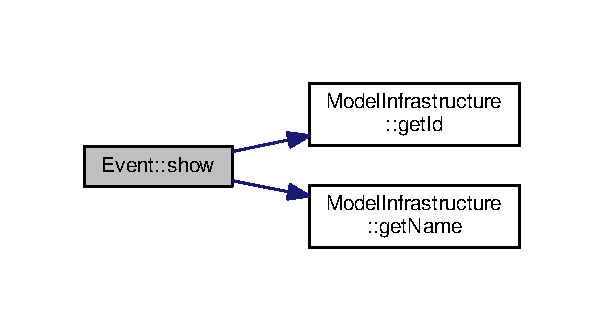
\includegraphics[width=290pt]{class_event_a640f132001d454af52cb0d0e20ebb856_cgraph}
\end{center}
\end{figure}




The documentation for this class was generated from the following files\-:\begin{DoxyCompactItemize}
\item 
\hyperlink{_event_8h}{Event.\-h}\item 
\hyperlink{_event_8cpp}{Event.\-cpp}\end{DoxyCompactItemize}

\hypertarget{class_fitter__if}{\section{Fitter\-\_\-if Class Reference}
\label{class_fitter__if}\index{Fitter\-\_\-if@{Fitter\-\_\-if}}
}


{\ttfamily \#include $<$Fitter\-\_\-if.\-h$>$}



Inheritance diagram for Fitter\-\_\-if\-:\nopagebreak
\begin{figure}[H]
\begin{center}
\leavevmode
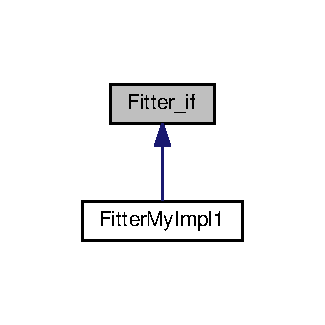
\includegraphics[width=156pt]{class_fitter__if__inherit__graph}
\end{center}
\end{figure}
\subsection*{Public Member Functions}
\begin{DoxyCompactItemize}
\item 
virtual bool \hyperlink{class_fitter__if_a53e98635fcdee314e8ade8089f41ddad}{is\-Normal\-Distributed} (double confidencelevel)=0
\item 
virtual void \hyperlink{class_fitter__if_adec53dfede4bdb31b175e57e6a2c2fc7}{fit\-Uniform} (double $\ast$sqrerror, double $\ast$min, double $\ast$max)=0
\item 
virtual void \hyperlink{class_fitter__if_a2bfc41c6a8044520aeafb2c5c71fe570}{fit\-Triangular} (double $\ast$sqrerror, double $\ast$min, double $\ast$mo, double $\ast$max)=0
\item 
virtual void \hyperlink{class_fitter__if_af95b4de00b7ed5d67b10d9ee458379bf}{fit\-Normal} (double $\ast$sqrerror, double $\ast$avg, double $\ast$stddev)=0
\item 
virtual void \hyperlink{class_fitter__if_a5ab5ac575b736bb720e6a40b334de5a3}{fit\-Expo} (double $\ast$sqrerror, double $\ast$avg1)=0
\item 
virtual void \hyperlink{class_fitter__if_aa46a5cd2d50d3cab34a719099e1058a1}{fit\-Erlang} (double $\ast$sqrerror, double $\ast$a, double $\ast$b, double $\ast$offset, double $\ast$mult)=0
\item 
virtual void \hyperlink{class_fitter__if_a686a7d540919b2e604df93b3049562d1}{fit\-Beta} (double $\ast$sqrerror, double $\ast$a, double $\ast$b, double $\ast$offset, double $\ast$mult)=0
\item 
virtual void \hyperlink{class_fitter__if_ae46e4cbb4354d6d06167aa498855d7ea}{fit\-Weibull} (double $\ast$sqrerror, double $\ast$a, double $\ast$b, double $\ast$offset, double $\ast$mult)=0
\item 
virtual void \hyperlink{class_fitter__if_a819a5ca8715ba4be30d2c7a3957aa467}{fit\-All} (double $\ast$sqrerror, std\-::string $\ast$name)=0
\item 
virtual void \hyperlink{class_fitter__if_aa2d2f13548a09a2f727a4190a6b9c2dd}{set\-Data\-Filename} (std\-::string data\-Filename)=0
\item 
virtual std\-::string \hyperlink{class_fitter__if_a3c6926020b1224a960890fe308abcc86}{get\-Data\-Filename} ()=0
\end{DoxyCompactItemize}


\subsection{Member Function Documentation}
\hypertarget{class_fitter__if_a819a5ca8715ba4be30d2c7a3957aa467}{\index{Fitter\-\_\-if@{Fitter\-\_\-if}!fit\-All@{fit\-All}}
\index{fit\-All@{fit\-All}!Fitter_if@{Fitter\-\_\-if}}
\subsubsection[{fit\-All}]{\setlength{\rightskip}{0pt plus 5cm}virtual void Fitter\-\_\-if\-::fit\-All (
\begin{DoxyParamCaption}
\item[{double $\ast$}]{sqrerror, }
\item[{std\-::string $\ast$}]{name}
\end{DoxyParamCaption}
)\hspace{0.3cm}{\ttfamily [pure virtual]}}}\label{class_fitter__if_a819a5ca8715ba4be30d2c7a3957aa467}


Implemented in \hyperlink{class_fitter_my_impl1_ad10f9269396cb86f2230edf652242f23}{Fitter\-My\-Impl1}.

\hypertarget{class_fitter__if_a686a7d540919b2e604df93b3049562d1}{\index{Fitter\-\_\-if@{Fitter\-\_\-if}!fit\-Beta@{fit\-Beta}}
\index{fit\-Beta@{fit\-Beta}!Fitter_if@{Fitter\-\_\-if}}
\subsubsection[{fit\-Beta}]{\setlength{\rightskip}{0pt plus 5cm}virtual void Fitter\-\_\-if\-::fit\-Beta (
\begin{DoxyParamCaption}
\item[{double $\ast$}]{sqrerror, }
\item[{double $\ast$}]{a, }
\item[{double $\ast$}]{b, }
\item[{double $\ast$}]{offset, }
\item[{double $\ast$}]{mult}
\end{DoxyParamCaption}
)\hspace{0.3cm}{\ttfamily [pure virtual]}}}\label{class_fitter__if_a686a7d540919b2e604df93b3049562d1}


Implemented in \hyperlink{class_fitter_my_impl1_acc9bcdffd5336751b197ed495c5826ca}{Fitter\-My\-Impl1}.

\hypertarget{class_fitter__if_aa46a5cd2d50d3cab34a719099e1058a1}{\index{Fitter\-\_\-if@{Fitter\-\_\-if}!fit\-Erlang@{fit\-Erlang}}
\index{fit\-Erlang@{fit\-Erlang}!Fitter_if@{Fitter\-\_\-if}}
\subsubsection[{fit\-Erlang}]{\setlength{\rightskip}{0pt plus 5cm}virtual void Fitter\-\_\-if\-::fit\-Erlang (
\begin{DoxyParamCaption}
\item[{double $\ast$}]{sqrerror, }
\item[{double $\ast$}]{a, }
\item[{double $\ast$}]{b, }
\item[{double $\ast$}]{offset, }
\item[{double $\ast$}]{mult}
\end{DoxyParamCaption}
)\hspace{0.3cm}{\ttfamily [pure virtual]}}}\label{class_fitter__if_aa46a5cd2d50d3cab34a719099e1058a1}


Implemented in \hyperlink{class_fitter_my_impl1_af5e7d08e466ae2154a97356939447f3c}{Fitter\-My\-Impl1}.

\hypertarget{class_fitter__if_a5ab5ac575b736bb720e6a40b334de5a3}{\index{Fitter\-\_\-if@{Fitter\-\_\-if}!fit\-Expo@{fit\-Expo}}
\index{fit\-Expo@{fit\-Expo}!Fitter_if@{Fitter\-\_\-if}}
\subsubsection[{fit\-Expo}]{\setlength{\rightskip}{0pt plus 5cm}virtual void Fitter\-\_\-if\-::fit\-Expo (
\begin{DoxyParamCaption}
\item[{double $\ast$}]{sqrerror, }
\item[{double $\ast$}]{avg1}
\end{DoxyParamCaption}
)\hspace{0.3cm}{\ttfamily [pure virtual]}}}\label{class_fitter__if_a5ab5ac575b736bb720e6a40b334de5a3}


Implemented in \hyperlink{class_fitter_my_impl1_aba4920314b8dcf17ee9d4f6d19ea48b2}{Fitter\-My\-Impl1}.

\hypertarget{class_fitter__if_af95b4de00b7ed5d67b10d9ee458379bf}{\index{Fitter\-\_\-if@{Fitter\-\_\-if}!fit\-Normal@{fit\-Normal}}
\index{fit\-Normal@{fit\-Normal}!Fitter_if@{Fitter\-\_\-if}}
\subsubsection[{fit\-Normal}]{\setlength{\rightskip}{0pt plus 5cm}virtual void Fitter\-\_\-if\-::fit\-Normal (
\begin{DoxyParamCaption}
\item[{double $\ast$}]{sqrerror, }
\item[{double $\ast$}]{avg, }
\item[{double $\ast$}]{stddev}
\end{DoxyParamCaption}
)\hspace{0.3cm}{\ttfamily [pure virtual]}}}\label{class_fitter__if_af95b4de00b7ed5d67b10d9ee458379bf}


Implemented in \hyperlink{class_fitter_my_impl1_a42ad0944837a2921674289c2ac264176}{Fitter\-My\-Impl1}.

\hypertarget{class_fitter__if_a2bfc41c6a8044520aeafb2c5c71fe570}{\index{Fitter\-\_\-if@{Fitter\-\_\-if}!fit\-Triangular@{fit\-Triangular}}
\index{fit\-Triangular@{fit\-Triangular}!Fitter_if@{Fitter\-\_\-if}}
\subsubsection[{fit\-Triangular}]{\setlength{\rightskip}{0pt plus 5cm}virtual void Fitter\-\_\-if\-::fit\-Triangular (
\begin{DoxyParamCaption}
\item[{double $\ast$}]{sqrerror, }
\item[{double $\ast$}]{min, }
\item[{double $\ast$}]{mo, }
\item[{double $\ast$}]{max}
\end{DoxyParamCaption}
)\hspace{0.3cm}{\ttfamily [pure virtual]}}}\label{class_fitter__if_a2bfc41c6a8044520aeafb2c5c71fe570}


Implemented in \hyperlink{class_fitter_my_impl1_a41a9b0e578a67a5bb33bb248388f5cb4}{Fitter\-My\-Impl1}.

\hypertarget{class_fitter__if_adec53dfede4bdb31b175e57e6a2c2fc7}{\index{Fitter\-\_\-if@{Fitter\-\_\-if}!fit\-Uniform@{fit\-Uniform}}
\index{fit\-Uniform@{fit\-Uniform}!Fitter_if@{Fitter\-\_\-if}}
\subsubsection[{fit\-Uniform}]{\setlength{\rightskip}{0pt plus 5cm}virtual void Fitter\-\_\-if\-::fit\-Uniform (
\begin{DoxyParamCaption}
\item[{double $\ast$}]{sqrerror, }
\item[{double $\ast$}]{min, }
\item[{double $\ast$}]{max}
\end{DoxyParamCaption}
)\hspace{0.3cm}{\ttfamily [pure virtual]}}}\label{class_fitter__if_adec53dfede4bdb31b175e57e6a2c2fc7}


Implemented in \hyperlink{class_fitter_my_impl1_adde8080641759eaea1d247d3c7436b1d}{Fitter\-My\-Impl1}.

\hypertarget{class_fitter__if_ae46e4cbb4354d6d06167aa498855d7ea}{\index{Fitter\-\_\-if@{Fitter\-\_\-if}!fit\-Weibull@{fit\-Weibull}}
\index{fit\-Weibull@{fit\-Weibull}!Fitter_if@{Fitter\-\_\-if}}
\subsubsection[{fit\-Weibull}]{\setlength{\rightskip}{0pt plus 5cm}virtual void Fitter\-\_\-if\-::fit\-Weibull (
\begin{DoxyParamCaption}
\item[{double $\ast$}]{sqrerror, }
\item[{double $\ast$}]{a, }
\item[{double $\ast$}]{b, }
\item[{double $\ast$}]{offset, }
\item[{double $\ast$}]{mult}
\end{DoxyParamCaption}
)\hspace{0.3cm}{\ttfamily [pure virtual]}}}\label{class_fitter__if_ae46e4cbb4354d6d06167aa498855d7ea}


Implemented in \hyperlink{class_fitter_my_impl1_a28bc8f7f558e4328bede20c941b6c32b}{Fitter\-My\-Impl1}.

\hypertarget{class_fitter__if_a3c6926020b1224a960890fe308abcc86}{\index{Fitter\-\_\-if@{Fitter\-\_\-if}!get\-Data\-Filename@{get\-Data\-Filename}}
\index{get\-Data\-Filename@{get\-Data\-Filename}!Fitter_if@{Fitter\-\_\-if}}
\subsubsection[{get\-Data\-Filename}]{\setlength{\rightskip}{0pt plus 5cm}virtual std\-::string Fitter\-\_\-if\-::get\-Data\-Filename (
\begin{DoxyParamCaption}
{}
\end{DoxyParamCaption}
)\hspace{0.3cm}{\ttfamily [pure virtual]}}}\label{class_fitter__if_a3c6926020b1224a960890fe308abcc86}


Implemented in \hyperlink{class_fitter_my_impl1_a7a9ea5c0a702ba2880dd3ed652f92030}{Fitter\-My\-Impl1}.

\hypertarget{class_fitter__if_a53e98635fcdee314e8ade8089f41ddad}{\index{Fitter\-\_\-if@{Fitter\-\_\-if}!is\-Normal\-Distributed@{is\-Normal\-Distributed}}
\index{is\-Normal\-Distributed@{is\-Normal\-Distributed}!Fitter_if@{Fitter\-\_\-if}}
\subsubsection[{is\-Normal\-Distributed}]{\setlength{\rightskip}{0pt plus 5cm}virtual bool Fitter\-\_\-if\-::is\-Normal\-Distributed (
\begin{DoxyParamCaption}
\item[{double}]{confidencelevel}
\end{DoxyParamCaption}
)\hspace{0.3cm}{\ttfamily [pure virtual]}}}\label{class_fitter__if_a53e98635fcdee314e8ade8089f41ddad}


Implemented in \hyperlink{class_fitter_my_impl1_abcb39383a71603a570d1e2c396c6b7ca}{Fitter\-My\-Impl1}.

\hypertarget{class_fitter__if_aa2d2f13548a09a2f727a4190a6b9c2dd}{\index{Fitter\-\_\-if@{Fitter\-\_\-if}!set\-Data\-Filename@{set\-Data\-Filename}}
\index{set\-Data\-Filename@{set\-Data\-Filename}!Fitter_if@{Fitter\-\_\-if}}
\subsubsection[{set\-Data\-Filename}]{\setlength{\rightskip}{0pt plus 5cm}virtual void Fitter\-\_\-if\-::set\-Data\-Filename (
\begin{DoxyParamCaption}
\item[{std\-::string}]{data\-Filename}
\end{DoxyParamCaption}
)\hspace{0.3cm}{\ttfamily [pure virtual]}}}\label{class_fitter__if_aa2d2f13548a09a2f727a4190a6b9c2dd}


Implemented in \hyperlink{class_fitter_my_impl1_a02c8f65838daa1f086586561aea6e4da}{Fitter\-My\-Impl1}.



The documentation for this class was generated from the following file\-:\begin{DoxyCompactItemize}
\item 
\hyperlink{_fitter__if_8h}{Fitter\-\_\-if.\-h}\end{DoxyCompactItemize}

\hypertarget{class_fitter_my_impl1}{\section{Fitter\-My\-Impl1 Class Reference}
\label{class_fitter_my_impl1}\index{Fitter\-My\-Impl1@{Fitter\-My\-Impl1}}
}


{\ttfamily \#include $<$Fitter\-My\-Impl1.\-h$>$}



Inheritance diagram for Fitter\-My\-Impl1\-:\nopagebreak
\begin{figure}[H]
\begin{center}
\leavevmode
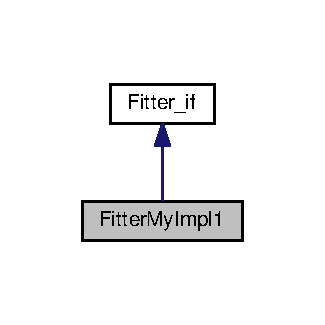
\includegraphics[width=156pt]{class_fitter_my_impl1__inherit__graph}
\end{center}
\end{figure}


Collaboration diagram for Fitter\-My\-Impl1\-:\nopagebreak
\begin{figure}[H]
\begin{center}
\leavevmode
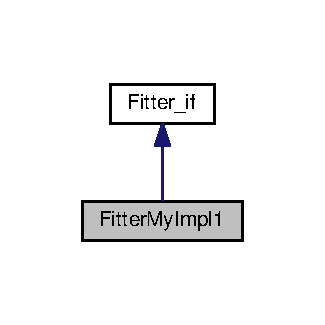
\includegraphics[width=156pt]{class_fitter_my_impl1__coll__graph}
\end{center}
\end{figure}
\subsection*{Public Member Functions}
\begin{DoxyCompactItemize}
\item 
\hyperlink{class_fitter_my_impl1_a9047919931ab66d267e9c91a378e7413}{Fitter\-My\-Impl1} ()
\item 
\hyperlink{class_fitter_my_impl1_a240ccdcb7aef045f1a31b554b990593a}{Fitter\-My\-Impl1} (const \hyperlink{class_fitter_my_impl1}{Fitter\-My\-Impl1} \&orig)
\item 
\hyperlink{class_fitter_my_impl1_a7097d3bca5ecc73393b54ef07973b841}{$\sim$\-Fitter\-My\-Impl1} ()
\item 
bool \hyperlink{class_fitter_my_impl1_abcb39383a71603a570d1e2c396c6b7ca}{is\-Normal\-Distributed} (double confidencelevel)
\item 
void \hyperlink{class_fitter_my_impl1_adde8080641759eaea1d247d3c7436b1d}{fit\-Uniform} (double $\ast$sqrerror, double $\ast$min, double $\ast$max)
\item 
void \hyperlink{class_fitter_my_impl1_a41a9b0e578a67a5bb33bb248388f5cb4}{fit\-Triangular} (double $\ast$sqrerror, double $\ast$min, double $\ast$mo, double $\ast$max)
\item 
void \hyperlink{class_fitter_my_impl1_a42ad0944837a2921674289c2ac264176}{fit\-Normal} (double $\ast$sqrerror, double $\ast$avg, double $\ast$stddev)
\item 
void \hyperlink{class_fitter_my_impl1_aba4920314b8dcf17ee9d4f6d19ea48b2}{fit\-Expo} (double $\ast$sqrerror, double $\ast$avg1)
\item 
void \hyperlink{class_fitter_my_impl1_af5e7d08e466ae2154a97356939447f3c}{fit\-Erlang} (double $\ast$sqrerror, double $\ast$a, double $\ast$b, double $\ast$offset, double $\ast$mult)
\item 
void \hyperlink{class_fitter_my_impl1_acc9bcdffd5336751b197ed495c5826ca}{fit\-Beta} (double $\ast$sqrerror, double $\ast$a, double $\ast$b, double $\ast$offset, double $\ast$mult)
\item 
void \hyperlink{class_fitter_my_impl1_a28bc8f7f558e4328bede20c941b6c32b}{fit\-Weibull} (double $\ast$sqrerror, double $\ast$a, double $\ast$b, double $\ast$offset, double $\ast$mult)
\item 
void \hyperlink{class_fitter_my_impl1_ad10f9269396cb86f2230edf652242f23}{fit\-All} (double $\ast$sqrerror, std\-::string $\ast$name)
\item 
void \hyperlink{class_fitter_my_impl1_a02c8f65838daa1f086586561aea6e4da}{set\-Data\-Filename} (std\-::string data\-Filename)
\item 
std\-::string \hyperlink{class_fitter_my_impl1_a7a9ea5c0a702ba2880dd3ed652f92030}{get\-Data\-Filename} ()
\end{DoxyCompactItemize}


\subsection{Constructor \& Destructor Documentation}
\hypertarget{class_fitter_my_impl1_a9047919931ab66d267e9c91a378e7413}{\index{Fitter\-My\-Impl1@{Fitter\-My\-Impl1}!Fitter\-My\-Impl1@{Fitter\-My\-Impl1}}
\index{Fitter\-My\-Impl1@{Fitter\-My\-Impl1}!FitterMyImpl1@{Fitter\-My\-Impl1}}
\subsubsection[{Fitter\-My\-Impl1}]{\setlength{\rightskip}{0pt plus 5cm}Fitter\-My\-Impl1\-::\-Fitter\-My\-Impl1 (
\begin{DoxyParamCaption}
{}
\end{DoxyParamCaption}
)}}\label{class_fitter_my_impl1_a9047919931ab66d267e9c91a378e7413}
\hypertarget{class_fitter_my_impl1_a240ccdcb7aef045f1a31b554b990593a}{\index{Fitter\-My\-Impl1@{Fitter\-My\-Impl1}!Fitter\-My\-Impl1@{Fitter\-My\-Impl1}}
\index{Fitter\-My\-Impl1@{Fitter\-My\-Impl1}!FitterMyImpl1@{Fitter\-My\-Impl1}}
\subsubsection[{Fitter\-My\-Impl1}]{\setlength{\rightskip}{0pt plus 5cm}Fitter\-My\-Impl1\-::\-Fitter\-My\-Impl1 (
\begin{DoxyParamCaption}
\item[{const {\bf Fitter\-My\-Impl1} \&}]{orig}
\end{DoxyParamCaption}
)}}\label{class_fitter_my_impl1_a240ccdcb7aef045f1a31b554b990593a}
\hypertarget{class_fitter_my_impl1_a7097d3bca5ecc73393b54ef07973b841}{\index{Fitter\-My\-Impl1@{Fitter\-My\-Impl1}!$\sim$\-Fitter\-My\-Impl1@{$\sim$\-Fitter\-My\-Impl1}}
\index{$\sim$\-Fitter\-My\-Impl1@{$\sim$\-Fitter\-My\-Impl1}!FitterMyImpl1@{Fitter\-My\-Impl1}}
\subsubsection[{$\sim$\-Fitter\-My\-Impl1}]{\setlength{\rightskip}{0pt plus 5cm}Fitter\-My\-Impl1\-::$\sim$\-Fitter\-My\-Impl1 (
\begin{DoxyParamCaption}
{}
\end{DoxyParamCaption}
)}}\label{class_fitter_my_impl1_a7097d3bca5ecc73393b54ef07973b841}


\subsection{Member Function Documentation}
\hypertarget{class_fitter_my_impl1_ad10f9269396cb86f2230edf652242f23}{\index{Fitter\-My\-Impl1@{Fitter\-My\-Impl1}!fit\-All@{fit\-All}}
\index{fit\-All@{fit\-All}!FitterMyImpl1@{Fitter\-My\-Impl1}}
\subsubsection[{fit\-All}]{\setlength{\rightskip}{0pt plus 5cm}void Fitter\-My\-Impl1\-::fit\-All (
\begin{DoxyParamCaption}
\item[{double $\ast$}]{sqrerror, }
\item[{std\-::string $\ast$}]{name}
\end{DoxyParamCaption}
)\hspace{0.3cm}{\ttfamily [virtual]}}}\label{class_fitter_my_impl1_ad10f9269396cb86f2230edf652242f23}


Implements \hyperlink{class_fitter__if_a819a5ca8715ba4be30d2c7a3957aa467}{Fitter\-\_\-if}.

\hypertarget{class_fitter_my_impl1_acc9bcdffd5336751b197ed495c5826ca}{\index{Fitter\-My\-Impl1@{Fitter\-My\-Impl1}!fit\-Beta@{fit\-Beta}}
\index{fit\-Beta@{fit\-Beta}!FitterMyImpl1@{Fitter\-My\-Impl1}}
\subsubsection[{fit\-Beta}]{\setlength{\rightskip}{0pt plus 5cm}void Fitter\-My\-Impl1\-::fit\-Beta (
\begin{DoxyParamCaption}
\item[{double $\ast$}]{sqrerror, }
\item[{double $\ast$}]{a, }
\item[{double $\ast$}]{b, }
\item[{double $\ast$}]{offset, }
\item[{double $\ast$}]{mult}
\end{DoxyParamCaption}
)\hspace{0.3cm}{\ttfamily [virtual]}}}\label{class_fitter_my_impl1_acc9bcdffd5336751b197ed495c5826ca}


Implements \hyperlink{class_fitter__if_a686a7d540919b2e604df93b3049562d1}{Fitter\-\_\-if}.

\hypertarget{class_fitter_my_impl1_af5e7d08e466ae2154a97356939447f3c}{\index{Fitter\-My\-Impl1@{Fitter\-My\-Impl1}!fit\-Erlang@{fit\-Erlang}}
\index{fit\-Erlang@{fit\-Erlang}!FitterMyImpl1@{Fitter\-My\-Impl1}}
\subsubsection[{fit\-Erlang}]{\setlength{\rightskip}{0pt plus 5cm}void Fitter\-My\-Impl1\-::fit\-Erlang (
\begin{DoxyParamCaption}
\item[{double $\ast$}]{sqrerror, }
\item[{double $\ast$}]{a, }
\item[{double $\ast$}]{b, }
\item[{double $\ast$}]{offset, }
\item[{double $\ast$}]{mult}
\end{DoxyParamCaption}
)\hspace{0.3cm}{\ttfamily [virtual]}}}\label{class_fitter_my_impl1_af5e7d08e466ae2154a97356939447f3c}


Implements \hyperlink{class_fitter__if_aa46a5cd2d50d3cab34a719099e1058a1}{Fitter\-\_\-if}.

\hypertarget{class_fitter_my_impl1_aba4920314b8dcf17ee9d4f6d19ea48b2}{\index{Fitter\-My\-Impl1@{Fitter\-My\-Impl1}!fit\-Expo@{fit\-Expo}}
\index{fit\-Expo@{fit\-Expo}!FitterMyImpl1@{Fitter\-My\-Impl1}}
\subsubsection[{fit\-Expo}]{\setlength{\rightskip}{0pt plus 5cm}void Fitter\-My\-Impl1\-::fit\-Expo (
\begin{DoxyParamCaption}
\item[{double $\ast$}]{sqrerror, }
\item[{double $\ast$}]{avg1}
\end{DoxyParamCaption}
)\hspace{0.3cm}{\ttfamily [virtual]}}}\label{class_fitter_my_impl1_aba4920314b8dcf17ee9d4f6d19ea48b2}


Implements \hyperlink{class_fitter__if_a5ab5ac575b736bb720e6a40b334de5a3}{Fitter\-\_\-if}.

\hypertarget{class_fitter_my_impl1_a42ad0944837a2921674289c2ac264176}{\index{Fitter\-My\-Impl1@{Fitter\-My\-Impl1}!fit\-Normal@{fit\-Normal}}
\index{fit\-Normal@{fit\-Normal}!FitterMyImpl1@{Fitter\-My\-Impl1}}
\subsubsection[{fit\-Normal}]{\setlength{\rightskip}{0pt plus 5cm}void Fitter\-My\-Impl1\-::fit\-Normal (
\begin{DoxyParamCaption}
\item[{double $\ast$}]{sqrerror, }
\item[{double $\ast$}]{avg, }
\item[{double $\ast$}]{stddev}
\end{DoxyParamCaption}
)\hspace{0.3cm}{\ttfamily [virtual]}}}\label{class_fitter_my_impl1_a42ad0944837a2921674289c2ac264176}


Implements \hyperlink{class_fitter__if_af95b4de00b7ed5d67b10d9ee458379bf}{Fitter\-\_\-if}.

\hypertarget{class_fitter_my_impl1_a41a9b0e578a67a5bb33bb248388f5cb4}{\index{Fitter\-My\-Impl1@{Fitter\-My\-Impl1}!fit\-Triangular@{fit\-Triangular}}
\index{fit\-Triangular@{fit\-Triangular}!FitterMyImpl1@{Fitter\-My\-Impl1}}
\subsubsection[{fit\-Triangular}]{\setlength{\rightskip}{0pt plus 5cm}void Fitter\-My\-Impl1\-::fit\-Triangular (
\begin{DoxyParamCaption}
\item[{double $\ast$}]{sqrerror, }
\item[{double $\ast$}]{min, }
\item[{double $\ast$}]{mo, }
\item[{double $\ast$}]{max}
\end{DoxyParamCaption}
)\hspace{0.3cm}{\ttfamily [virtual]}}}\label{class_fitter_my_impl1_a41a9b0e578a67a5bb33bb248388f5cb4}


Implements \hyperlink{class_fitter__if_a2bfc41c6a8044520aeafb2c5c71fe570}{Fitter\-\_\-if}.

\hypertarget{class_fitter_my_impl1_adde8080641759eaea1d247d3c7436b1d}{\index{Fitter\-My\-Impl1@{Fitter\-My\-Impl1}!fit\-Uniform@{fit\-Uniform}}
\index{fit\-Uniform@{fit\-Uniform}!FitterMyImpl1@{Fitter\-My\-Impl1}}
\subsubsection[{fit\-Uniform}]{\setlength{\rightskip}{0pt plus 5cm}void Fitter\-My\-Impl1\-::fit\-Uniform (
\begin{DoxyParamCaption}
\item[{double $\ast$}]{sqrerror, }
\item[{double $\ast$}]{min, }
\item[{double $\ast$}]{max}
\end{DoxyParamCaption}
)\hspace{0.3cm}{\ttfamily [virtual]}}}\label{class_fitter_my_impl1_adde8080641759eaea1d247d3c7436b1d}


Implements \hyperlink{class_fitter__if_adec53dfede4bdb31b175e57e6a2c2fc7}{Fitter\-\_\-if}.

\hypertarget{class_fitter_my_impl1_a28bc8f7f558e4328bede20c941b6c32b}{\index{Fitter\-My\-Impl1@{Fitter\-My\-Impl1}!fit\-Weibull@{fit\-Weibull}}
\index{fit\-Weibull@{fit\-Weibull}!FitterMyImpl1@{Fitter\-My\-Impl1}}
\subsubsection[{fit\-Weibull}]{\setlength{\rightskip}{0pt plus 5cm}void Fitter\-My\-Impl1\-::fit\-Weibull (
\begin{DoxyParamCaption}
\item[{double $\ast$}]{sqrerror, }
\item[{double $\ast$}]{a, }
\item[{double $\ast$}]{b, }
\item[{double $\ast$}]{offset, }
\item[{double $\ast$}]{mult}
\end{DoxyParamCaption}
)\hspace{0.3cm}{\ttfamily [virtual]}}}\label{class_fitter_my_impl1_a28bc8f7f558e4328bede20c941b6c32b}


Implements \hyperlink{class_fitter__if_ae46e4cbb4354d6d06167aa498855d7ea}{Fitter\-\_\-if}.

\hypertarget{class_fitter_my_impl1_a7a9ea5c0a702ba2880dd3ed652f92030}{\index{Fitter\-My\-Impl1@{Fitter\-My\-Impl1}!get\-Data\-Filename@{get\-Data\-Filename}}
\index{get\-Data\-Filename@{get\-Data\-Filename}!FitterMyImpl1@{Fitter\-My\-Impl1}}
\subsubsection[{get\-Data\-Filename}]{\setlength{\rightskip}{0pt plus 5cm}std\-::string Fitter\-My\-Impl1\-::get\-Data\-Filename (
\begin{DoxyParamCaption}
{}
\end{DoxyParamCaption}
)\hspace{0.3cm}{\ttfamily [virtual]}}}\label{class_fitter_my_impl1_a7a9ea5c0a702ba2880dd3ed652f92030}


Implements \hyperlink{class_fitter__if_a3c6926020b1224a960890fe308abcc86}{Fitter\-\_\-if}.

\hypertarget{class_fitter_my_impl1_abcb39383a71603a570d1e2c396c6b7ca}{\index{Fitter\-My\-Impl1@{Fitter\-My\-Impl1}!is\-Normal\-Distributed@{is\-Normal\-Distributed}}
\index{is\-Normal\-Distributed@{is\-Normal\-Distributed}!FitterMyImpl1@{Fitter\-My\-Impl1}}
\subsubsection[{is\-Normal\-Distributed}]{\setlength{\rightskip}{0pt plus 5cm}bool Fitter\-My\-Impl1\-::is\-Normal\-Distributed (
\begin{DoxyParamCaption}
\item[{double}]{confidencelevel}
\end{DoxyParamCaption}
)\hspace{0.3cm}{\ttfamily [virtual]}}}\label{class_fitter_my_impl1_abcb39383a71603a570d1e2c396c6b7ca}


Implements \hyperlink{class_fitter__if_a53e98635fcdee314e8ade8089f41ddad}{Fitter\-\_\-if}.

\hypertarget{class_fitter_my_impl1_a02c8f65838daa1f086586561aea6e4da}{\index{Fitter\-My\-Impl1@{Fitter\-My\-Impl1}!set\-Data\-Filename@{set\-Data\-Filename}}
\index{set\-Data\-Filename@{set\-Data\-Filename}!FitterMyImpl1@{Fitter\-My\-Impl1}}
\subsubsection[{set\-Data\-Filename}]{\setlength{\rightskip}{0pt plus 5cm}void Fitter\-My\-Impl1\-::set\-Data\-Filename (
\begin{DoxyParamCaption}
\item[{std\-::string}]{data\-Filename}
\end{DoxyParamCaption}
)\hspace{0.3cm}{\ttfamily [virtual]}}}\label{class_fitter_my_impl1_a02c8f65838daa1f086586561aea6e4da}


Implements \hyperlink{class_fitter__if_aa2d2f13548a09a2f727a4190a6b9c2dd}{Fitter\-\_\-if}.



The documentation for this class was generated from the following files\-:\begin{DoxyCompactItemize}
\item 
\hyperlink{_fitter_my_impl1_8h}{Fitter\-My\-Impl1.\-h}\item 
\hyperlink{_fitter_my_impl1_8cpp}{Fitter\-My\-Impl1.\-cpp}\end{DoxyCompactItemize}

\hypertarget{class_hypothesis_tester__if}{\section{Hypothesis\-Tester\-\_\-if Class Reference}
\label{class_hypothesis_tester__if}\index{Hypothesis\-Tester\-\_\-if@{Hypothesis\-Tester\-\_\-if}}
}


{\ttfamily \#include $<$Hypothesis\-Tester\-\_\-if.\-h$>$}



Inheritance diagram for Hypothesis\-Tester\-\_\-if\-:\nopagebreak
\begin{figure}[H]
\begin{center}
\leavevmode
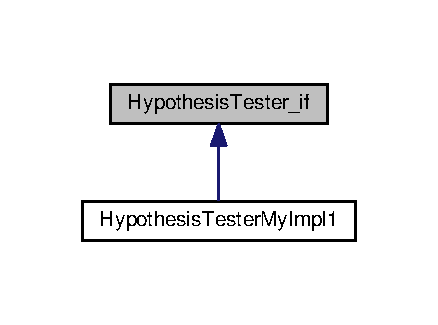
\includegraphics[width=210pt]{class_hypothesis_tester__if__inherit__graph}
\end{center}
\end{figure}
\subsection*{Public Types}
\begin{DoxyCompactItemize}
\item 
enum \hyperlink{class_hypothesis_tester__if_a89153ff990252f9f79856a2f2532c349}{H1\-Comparition} \{ \hyperlink{class_hypothesis_tester__if_a89153ff990252f9f79856a2f2532c349a58aba9f031dcbe91654e790416d84969}{L\-E\-S\-S\-\_\-\-T\-H\-A\-N} = 1, 
\hyperlink{class_hypothesis_tester__if_a89153ff990252f9f79856a2f2532c349a42d8b143727dc6856dddb0d0ce94c791}{E\-Q\-U\-A\-L} = 2, 
\hyperlink{class_hypothesis_tester__if_a89153ff990252f9f79856a2f2532c349acf8c0147414ce2a7cfdc8b26854464f8}{D\-I\-F\-F\-E\-R\-E\-N\-T} = 3, 
\hyperlink{class_hypothesis_tester__if_a89153ff990252f9f79856a2f2532c349ad0539d107f27b07e600a3c46da5b1934}{G\-R\-E\-A\-T\-E\-R\-\_\-\-T\-H\-A\-N} = 4
 \}
\end{DoxyCompactItemize}
\subsection*{Public Member Functions}
\begin{DoxyCompactItemize}
\item 
virtual bool \hyperlink{class_hypothesis_tester__if_a00a01e530acaf3f4db644b439c1c162e}{test\-Average} (double confidencelevel, double avg, \hyperlink{class_hypothesis_tester__if_a89153ff990252f9f79856a2f2532c349}{H1\-Comparition} comp)=0
\item 
virtual bool \hyperlink{class_hypothesis_tester__if_a9a07fdf3648371e4595acb3599f7b03b}{test\-Proportion} (double confidencelevel, double prop, \hyperlink{class_hypothesis_tester__if_a89153ff990252f9f79856a2f2532c349}{H1\-Comparition} comp)=0
\item 
virtual bool \hyperlink{class_hypothesis_tester__if_a1734abfa4bd0c3e8fc67c96172aca728}{test\-Variance} (double confidencelevel, double var, \hyperlink{class_hypothesis_tester__if_a89153ff990252f9f79856a2f2532c349}{H1\-Comparition} comp)=0
\item 
virtual bool \hyperlink{class_hypothesis_tester__if_a0c0314bc8ff8bef239583f2c8af4ed56}{test\-Average} (double confidencelevel, std\-::string second\-Population\-Data\-Filename, \hyperlink{class_hypothesis_tester__if_a89153ff990252f9f79856a2f2532c349}{H1\-Comparition} comp)=0
\item 
virtual bool \hyperlink{class_hypothesis_tester__if_a10b193007a3fde816120b32903241336}{test\-Proportion} (double confidencelevel, std\-::string second\-Population\-Data\-Filename, \hyperlink{class_hypothesis_tester__if_a89153ff990252f9f79856a2f2532c349}{H1\-Comparition} comp)=0
\item 
virtual bool \hyperlink{class_hypothesis_tester__if_ad2360392ccf3858da38092448152c33d}{test\-Variance} (double confidencelevel, std\-::string second\-Population\-Data\-Filename, \hyperlink{class_hypothesis_tester__if_a89153ff990252f9f79856a2f2532c349}{H1\-Comparition} comp)=0
\item 
virtual void \hyperlink{class_hypothesis_tester__if_ae7cfc801a3c0206844e3bc73e0b4234a}{set\-Data\-Filename} (std\-::string data\-Filename)=0
\item 
virtual std\-::string \hyperlink{class_hypothesis_tester__if_a37b02ea209d8f6b566af9e2fff6511cc}{get\-Data\-Filename} ()=0
\end{DoxyCompactItemize}


\subsection{Detailed Description}
Interface for parametric hypothesis tests based on a datafile. 

\subsection{Member Enumeration Documentation}
\hypertarget{class_hypothesis_tester__if_a89153ff990252f9f79856a2f2532c349}{\index{Hypothesis\-Tester\-\_\-if@{Hypothesis\-Tester\-\_\-if}!H1\-Comparition@{H1\-Comparition}}
\index{H1\-Comparition@{H1\-Comparition}!HypothesisTester_if@{Hypothesis\-Tester\-\_\-if}}
\subsubsection[{H1\-Comparition}]{\setlength{\rightskip}{0pt plus 5cm}enum {\bf Hypothesis\-Tester\-\_\-if\-::\-H1\-Comparition}}}\label{class_hypothesis_tester__if_a89153ff990252f9f79856a2f2532c349}
\begin{Desc}
\item[Enumerator]\par
\begin{description}
\index{L\-E\-S\-S\-\_\-\-T\-H\-A\-N@{L\-E\-S\-S\-\_\-\-T\-H\-A\-N}!Hypothesis\-Tester\-\_\-if@{Hypothesis\-Tester\-\_\-if}}\index{Hypothesis\-Tester\-\_\-if@{Hypothesis\-Tester\-\_\-if}!L\-E\-S\-S\-\_\-\-T\-H\-A\-N@{L\-E\-S\-S\-\_\-\-T\-H\-A\-N}}\item[{\em 
\hypertarget{class_hypothesis_tester__if_a89153ff990252f9f79856a2f2532c349a58aba9f031dcbe91654e790416d84969}{L\-E\-S\-S\-\_\-\-T\-H\-A\-N}\label{class_hypothesis_tester__if_a89153ff990252f9f79856a2f2532c349a58aba9f031dcbe91654e790416d84969}
}]\index{E\-Q\-U\-A\-L@{E\-Q\-U\-A\-L}!Hypothesis\-Tester\-\_\-if@{Hypothesis\-Tester\-\_\-if}}\index{Hypothesis\-Tester\-\_\-if@{Hypothesis\-Tester\-\_\-if}!E\-Q\-U\-A\-L@{E\-Q\-U\-A\-L}}\item[{\em 
\hypertarget{class_hypothesis_tester__if_a89153ff990252f9f79856a2f2532c349a42d8b143727dc6856dddb0d0ce94c791}{E\-Q\-U\-A\-L}\label{class_hypothesis_tester__if_a89153ff990252f9f79856a2f2532c349a42d8b143727dc6856dddb0d0ce94c791}
}]\index{D\-I\-F\-F\-E\-R\-E\-N\-T@{D\-I\-F\-F\-E\-R\-E\-N\-T}!Hypothesis\-Tester\-\_\-if@{Hypothesis\-Tester\-\_\-if}}\index{Hypothesis\-Tester\-\_\-if@{Hypothesis\-Tester\-\_\-if}!D\-I\-F\-F\-E\-R\-E\-N\-T@{D\-I\-F\-F\-E\-R\-E\-N\-T}}\item[{\em 
\hypertarget{class_hypothesis_tester__if_a89153ff990252f9f79856a2f2532c349acf8c0147414ce2a7cfdc8b26854464f8}{D\-I\-F\-F\-E\-R\-E\-N\-T}\label{class_hypothesis_tester__if_a89153ff990252f9f79856a2f2532c349acf8c0147414ce2a7cfdc8b26854464f8}
}]\index{G\-R\-E\-A\-T\-E\-R\-\_\-\-T\-H\-A\-N@{G\-R\-E\-A\-T\-E\-R\-\_\-\-T\-H\-A\-N}!Hypothesis\-Tester\-\_\-if@{Hypothesis\-Tester\-\_\-if}}\index{Hypothesis\-Tester\-\_\-if@{Hypothesis\-Tester\-\_\-if}!G\-R\-E\-A\-T\-E\-R\-\_\-\-T\-H\-A\-N@{G\-R\-E\-A\-T\-E\-R\-\_\-\-T\-H\-A\-N}}\item[{\em 
\hypertarget{class_hypothesis_tester__if_a89153ff990252f9f79856a2f2532c349ad0539d107f27b07e600a3c46da5b1934}{G\-R\-E\-A\-T\-E\-R\-\_\-\-T\-H\-A\-N}\label{class_hypothesis_tester__if_a89153ff990252f9f79856a2f2532c349ad0539d107f27b07e600a3c46da5b1934}
}]\end{description}
\end{Desc}


\subsection{Member Function Documentation}
\hypertarget{class_hypothesis_tester__if_a37b02ea209d8f6b566af9e2fff6511cc}{\index{Hypothesis\-Tester\-\_\-if@{Hypothesis\-Tester\-\_\-if}!get\-Data\-Filename@{get\-Data\-Filename}}
\index{get\-Data\-Filename@{get\-Data\-Filename}!HypothesisTester_if@{Hypothesis\-Tester\-\_\-if}}
\subsubsection[{get\-Data\-Filename}]{\setlength{\rightskip}{0pt plus 5cm}virtual std\-::string Hypothesis\-Tester\-\_\-if\-::get\-Data\-Filename (
\begin{DoxyParamCaption}
{}
\end{DoxyParamCaption}
)\hspace{0.3cm}{\ttfamily [pure virtual]}}}\label{class_hypothesis_tester__if_a37b02ea209d8f6b566af9e2fff6511cc}


Implemented in \hyperlink{class_hypothesis_tester_my_impl1_a78fc8e7ab09108a7c7698cc3a182b9d7}{Hypothesis\-Tester\-My\-Impl1}.

\hypertarget{class_hypothesis_tester__if_ae7cfc801a3c0206844e3bc73e0b4234a}{\index{Hypothesis\-Tester\-\_\-if@{Hypothesis\-Tester\-\_\-if}!set\-Data\-Filename@{set\-Data\-Filename}}
\index{set\-Data\-Filename@{set\-Data\-Filename}!HypothesisTester_if@{Hypothesis\-Tester\-\_\-if}}
\subsubsection[{set\-Data\-Filename}]{\setlength{\rightskip}{0pt plus 5cm}virtual void Hypothesis\-Tester\-\_\-if\-::set\-Data\-Filename (
\begin{DoxyParamCaption}
\item[{std\-::string}]{data\-Filename}
\end{DoxyParamCaption}
)\hspace{0.3cm}{\ttfamily [pure virtual]}}}\label{class_hypothesis_tester__if_ae7cfc801a3c0206844e3bc73e0b4234a}


Implemented in \hyperlink{class_hypothesis_tester_my_impl1_a96347967e7fb3ed8760d517b6dea9438}{Hypothesis\-Tester\-My\-Impl1}.

\hypertarget{class_hypothesis_tester__if_a00a01e530acaf3f4db644b439c1c162e}{\index{Hypothesis\-Tester\-\_\-if@{Hypothesis\-Tester\-\_\-if}!test\-Average@{test\-Average}}
\index{test\-Average@{test\-Average}!HypothesisTester_if@{Hypothesis\-Tester\-\_\-if}}
\subsubsection[{test\-Average}]{\setlength{\rightskip}{0pt plus 5cm}virtual bool Hypothesis\-Tester\-\_\-if\-::test\-Average (
\begin{DoxyParamCaption}
\item[{double}]{confidencelevel, }
\item[{double}]{avg, }
\item[{{\bf H1\-Comparition}}]{comp}
\end{DoxyParamCaption}
)\hspace{0.3cm}{\ttfamily [pure virtual]}}}\label{class_hypothesis_tester__if_a00a01e530acaf3f4db644b439c1c162e}


Implemented in \hyperlink{class_hypothesis_tester_my_impl1_ae221c4d7e9144d9ecdcb604c778ba0e8}{Hypothesis\-Tester\-My\-Impl1}.

\hypertarget{class_hypothesis_tester__if_a0c0314bc8ff8bef239583f2c8af4ed56}{\index{Hypothesis\-Tester\-\_\-if@{Hypothesis\-Tester\-\_\-if}!test\-Average@{test\-Average}}
\index{test\-Average@{test\-Average}!HypothesisTester_if@{Hypothesis\-Tester\-\_\-if}}
\subsubsection[{test\-Average}]{\setlength{\rightskip}{0pt plus 5cm}virtual bool Hypothesis\-Tester\-\_\-if\-::test\-Average (
\begin{DoxyParamCaption}
\item[{double}]{confidencelevel, }
\item[{std\-::string}]{second\-Population\-Data\-Filename, }
\item[{{\bf H1\-Comparition}}]{comp}
\end{DoxyParamCaption}
)\hspace{0.3cm}{\ttfamily [pure virtual]}}}\label{class_hypothesis_tester__if_a0c0314bc8ff8bef239583f2c8af4ed56}


Implemented in \hyperlink{class_hypothesis_tester_my_impl1_a0cfde7f4c69ea260350257b0c9c93c37}{Hypothesis\-Tester\-My\-Impl1}.

\hypertarget{class_hypothesis_tester__if_a9a07fdf3648371e4595acb3599f7b03b}{\index{Hypothesis\-Tester\-\_\-if@{Hypothesis\-Tester\-\_\-if}!test\-Proportion@{test\-Proportion}}
\index{test\-Proportion@{test\-Proportion}!HypothesisTester_if@{Hypothesis\-Tester\-\_\-if}}
\subsubsection[{test\-Proportion}]{\setlength{\rightskip}{0pt plus 5cm}virtual bool Hypothesis\-Tester\-\_\-if\-::test\-Proportion (
\begin{DoxyParamCaption}
\item[{double}]{confidencelevel, }
\item[{double}]{prop, }
\item[{{\bf H1\-Comparition}}]{comp}
\end{DoxyParamCaption}
)\hspace{0.3cm}{\ttfamily [pure virtual]}}}\label{class_hypothesis_tester__if_a9a07fdf3648371e4595acb3599f7b03b}


Implemented in \hyperlink{class_hypothesis_tester_my_impl1_a1adf16a900ed4c8b8296a9516877c38b}{Hypothesis\-Tester\-My\-Impl1}.

\hypertarget{class_hypothesis_tester__if_a10b193007a3fde816120b32903241336}{\index{Hypothesis\-Tester\-\_\-if@{Hypothesis\-Tester\-\_\-if}!test\-Proportion@{test\-Proportion}}
\index{test\-Proportion@{test\-Proportion}!HypothesisTester_if@{Hypothesis\-Tester\-\_\-if}}
\subsubsection[{test\-Proportion}]{\setlength{\rightskip}{0pt plus 5cm}virtual bool Hypothesis\-Tester\-\_\-if\-::test\-Proportion (
\begin{DoxyParamCaption}
\item[{double}]{confidencelevel, }
\item[{std\-::string}]{second\-Population\-Data\-Filename, }
\item[{{\bf H1\-Comparition}}]{comp}
\end{DoxyParamCaption}
)\hspace{0.3cm}{\ttfamily [pure virtual]}}}\label{class_hypothesis_tester__if_a10b193007a3fde816120b32903241336}


Implemented in \hyperlink{class_hypothesis_tester_my_impl1_a13d8ceafa5c23714105f7deae83b5b2e}{Hypothesis\-Tester\-My\-Impl1}.

\hypertarget{class_hypothesis_tester__if_a1734abfa4bd0c3e8fc67c96172aca728}{\index{Hypothesis\-Tester\-\_\-if@{Hypothesis\-Tester\-\_\-if}!test\-Variance@{test\-Variance}}
\index{test\-Variance@{test\-Variance}!HypothesisTester_if@{Hypothesis\-Tester\-\_\-if}}
\subsubsection[{test\-Variance}]{\setlength{\rightskip}{0pt plus 5cm}virtual bool Hypothesis\-Tester\-\_\-if\-::test\-Variance (
\begin{DoxyParamCaption}
\item[{double}]{confidencelevel, }
\item[{double}]{var, }
\item[{{\bf H1\-Comparition}}]{comp}
\end{DoxyParamCaption}
)\hspace{0.3cm}{\ttfamily [pure virtual]}}}\label{class_hypothesis_tester__if_a1734abfa4bd0c3e8fc67c96172aca728}


Implemented in \hyperlink{class_hypothesis_tester_my_impl1_a6aca02089c37992e8a6761807a5a127c}{Hypothesis\-Tester\-My\-Impl1}.

\hypertarget{class_hypothesis_tester__if_ad2360392ccf3858da38092448152c33d}{\index{Hypothesis\-Tester\-\_\-if@{Hypothesis\-Tester\-\_\-if}!test\-Variance@{test\-Variance}}
\index{test\-Variance@{test\-Variance}!HypothesisTester_if@{Hypothesis\-Tester\-\_\-if}}
\subsubsection[{test\-Variance}]{\setlength{\rightskip}{0pt plus 5cm}virtual bool Hypothesis\-Tester\-\_\-if\-::test\-Variance (
\begin{DoxyParamCaption}
\item[{double}]{confidencelevel, }
\item[{std\-::string}]{second\-Population\-Data\-Filename, }
\item[{{\bf H1\-Comparition}}]{comp}
\end{DoxyParamCaption}
)\hspace{0.3cm}{\ttfamily [pure virtual]}}}\label{class_hypothesis_tester__if_ad2360392ccf3858da38092448152c33d}


Implemented in \hyperlink{class_hypothesis_tester_my_impl1_aea5e966244b773179262205369d496d9}{Hypothesis\-Tester\-My\-Impl1}.



The documentation for this class was generated from the following file\-:\begin{DoxyCompactItemize}
\item 
\hyperlink{_hypothesis_tester__if_8h}{Hypothesis\-Tester\-\_\-if.\-h}\end{DoxyCompactItemize}

\hypertarget{class_hypothesis_tester_my_impl1}{\section{Hypothesis\-Tester\-My\-Impl1 Class Reference}
\label{class_hypothesis_tester_my_impl1}\index{Hypothesis\-Tester\-My\-Impl1@{Hypothesis\-Tester\-My\-Impl1}}
}


{\ttfamily \#include $<$Hypothesis\-Tester\-My\-Impl1.\-h$>$}



Inheritance diagram for Hypothesis\-Tester\-My\-Impl1\-:\nopagebreak
\begin{figure}[H]
\begin{center}
\leavevmode
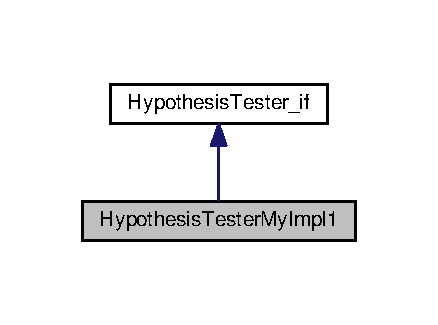
\includegraphics[width=210pt]{class_hypothesis_tester_my_impl1__inherit__graph}
\end{center}
\end{figure}


Collaboration diagram for Hypothesis\-Tester\-My\-Impl1\-:\nopagebreak
\begin{figure}[H]
\begin{center}
\leavevmode
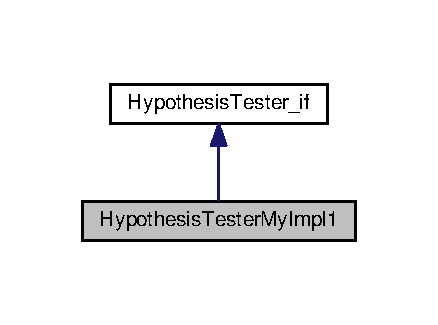
\includegraphics[width=210pt]{class_hypothesis_tester_my_impl1__coll__graph}
\end{center}
\end{figure}
\subsection*{Public Member Functions}
\begin{DoxyCompactItemize}
\item 
\hyperlink{class_hypothesis_tester_my_impl1_a1bc5f7e6d6a8f823e631b556f97179b9}{Hypothesis\-Tester\-My\-Impl1} ()
\item 
\hyperlink{class_hypothesis_tester_my_impl1_ac077c15369998d214ed4fda9a96ad046}{Hypothesis\-Tester\-My\-Impl1} (const \hyperlink{class_hypothesis_tester_my_impl1}{Hypothesis\-Tester\-My\-Impl1} \&orig)
\item 
\hyperlink{class_hypothesis_tester_my_impl1_a759939644e86036f014dae86e54e7297}{$\sim$\-Hypothesis\-Tester\-My\-Impl1} ()
\item 
bool \hyperlink{class_hypothesis_tester_my_impl1_ae221c4d7e9144d9ecdcb604c778ba0e8}{test\-Average} (double confidencelevel, double avg, \hyperlink{class_hypothesis_tester__if_a89153ff990252f9f79856a2f2532c349}{H1\-Comparition} comp)
\item 
bool \hyperlink{class_hypothesis_tester_my_impl1_a1adf16a900ed4c8b8296a9516877c38b}{test\-Proportion} (double confidencelevel, double prop, \hyperlink{class_hypothesis_tester__if_a89153ff990252f9f79856a2f2532c349}{H1\-Comparition} comp)
\item 
bool \hyperlink{class_hypothesis_tester_my_impl1_a6aca02089c37992e8a6761807a5a127c}{test\-Variance} (double confidencelevel, double var, \hyperlink{class_hypothesis_tester__if_a89153ff990252f9f79856a2f2532c349}{H1\-Comparition} comp)
\item 
bool \hyperlink{class_hypothesis_tester_my_impl1_a0cfde7f4c69ea260350257b0c9c93c37}{test\-Average} (double confidencelevel, std\-::string second\-Population\-Data\-Filename, \hyperlink{class_hypothesis_tester__if_a89153ff990252f9f79856a2f2532c349}{H1\-Comparition} comp)
\item 
bool \hyperlink{class_hypothesis_tester_my_impl1_a13d8ceafa5c23714105f7deae83b5b2e}{test\-Proportion} (double confidencelevel, std\-::string second\-Population\-Data\-Filename, \hyperlink{class_hypothesis_tester__if_a89153ff990252f9f79856a2f2532c349}{H1\-Comparition} comp)
\item 
bool \hyperlink{class_hypothesis_tester_my_impl1_aea5e966244b773179262205369d496d9}{test\-Variance} (double confidencelevel, std\-::string second\-Population\-Data\-Filename, \hyperlink{class_hypothesis_tester__if_a89153ff990252f9f79856a2f2532c349}{H1\-Comparition} comp)
\item 
void \hyperlink{class_hypothesis_tester_my_impl1_a96347967e7fb3ed8760d517b6dea9438}{set\-Data\-Filename} (std\-::string data\-Filename)
\item 
std\-::string \hyperlink{class_hypothesis_tester_my_impl1_a78fc8e7ab09108a7c7698cc3a182b9d7}{get\-Data\-Filename} ()
\end{DoxyCompactItemize}
\subsection*{Additional Inherited Members}


\subsection{Constructor \& Destructor Documentation}
\hypertarget{class_hypothesis_tester_my_impl1_a1bc5f7e6d6a8f823e631b556f97179b9}{\index{Hypothesis\-Tester\-My\-Impl1@{Hypothesis\-Tester\-My\-Impl1}!Hypothesis\-Tester\-My\-Impl1@{Hypothesis\-Tester\-My\-Impl1}}
\index{Hypothesis\-Tester\-My\-Impl1@{Hypothesis\-Tester\-My\-Impl1}!HypothesisTesterMyImpl1@{Hypothesis\-Tester\-My\-Impl1}}
\subsubsection[{Hypothesis\-Tester\-My\-Impl1}]{\setlength{\rightskip}{0pt plus 5cm}Hypothesis\-Tester\-My\-Impl1\-::\-Hypothesis\-Tester\-My\-Impl1 (
\begin{DoxyParamCaption}
{}
\end{DoxyParamCaption}
)}}\label{class_hypothesis_tester_my_impl1_a1bc5f7e6d6a8f823e631b556f97179b9}
\hypertarget{class_hypothesis_tester_my_impl1_ac077c15369998d214ed4fda9a96ad046}{\index{Hypothesis\-Tester\-My\-Impl1@{Hypothesis\-Tester\-My\-Impl1}!Hypothesis\-Tester\-My\-Impl1@{Hypothesis\-Tester\-My\-Impl1}}
\index{Hypothesis\-Tester\-My\-Impl1@{Hypothesis\-Tester\-My\-Impl1}!HypothesisTesterMyImpl1@{Hypothesis\-Tester\-My\-Impl1}}
\subsubsection[{Hypothesis\-Tester\-My\-Impl1}]{\setlength{\rightskip}{0pt plus 5cm}Hypothesis\-Tester\-My\-Impl1\-::\-Hypothesis\-Tester\-My\-Impl1 (
\begin{DoxyParamCaption}
\item[{const {\bf Hypothesis\-Tester\-My\-Impl1} \&}]{orig}
\end{DoxyParamCaption}
)}}\label{class_hypothesis_tester_my_impl1_ac077c15369998d214ed4fda9a96ad046}
\hypertarget{class_hypothesis_tester_my_impl1_a759939644e86036f014dae86e54e7297}{\index{Hypothesis\-Tester\-My\-Impl1@{Hypothesis\-Tester\-My\-Impl1}!$\sim$\-Hypothesis\-Tester\-My\-Impl1@{$\sim$\-Hypothesis\-Tester\-My\-Impl1}}
\index{$\sim$\-Hypothesis\-Tester\-My\-Impl1@{$\sim$\-Hypothesis\-Tester\-My\-Impl1}!HypothesisTesterMyImpl1@{Hypothesis\-Tester\-My\-Impl1}}
\subsubsection[{$\sim$\-Hypothesis\-Tester\-My\-Impl1}]{\setlength{\rightskip}{0pt plus 5cm}Hypothesis\-Tester\-My\-Impl1\-::$\sim$\-Hypothesis\-Tester\-My\-Impl1 (
\begin{DoxyParamCaption}
{}
\end{DoxyParamCaption}
)}}\label{class_hypothesis_tester_my_impl1_a759939644e86036f014dae86e54e7297}


\subsection{Member Function Documentation}
\hypertarget{class_hypothesis_tester_my_impl1_a78fc8e7ab09108a7c7698cc3a182b9d7}{\index{Hypothesis\-Tester\-My\-Impl1@{Hypothesis\-Tester\-My\-Impl1}!get\-Data\-Filename@{get\-Data\-Filename}}
\index{get\-Data\-Filename@{get\-Data\-Filename}!HypothesisTesterMyImpl1@{Hypothesis\-Tester\-My\-Impl1}}
\subsubsection[{get\-Data\-Filename}]{\setlength{\rightskip}{0pt plus 5cm}std\-::string Hypothesis\-Tester\-My\-Impl1\-::get\-Data\-Filename (
\begin{DoxyParamCaption}
{}
\end{DoxyParamCaption}
)\hspace{0.3cm}{\ttfamily [virtual]}}}\label{class_hypothesis_tester_my_impl1_a78fc8e7ab09108a7c7698cc3a182b9d7}


Implements \hyperlink{class_hypothesis_tester__if_a37b02ea209d8f6b566af9e2fff6511cc}{Hypothesis\-Tester\-\_\-if}.

\hypertarget{class_hypothesis_tester_my_impl1_a96347967e7fb3ed8760d517b6dea9438}{\index{Hypothesis\-Tester\-My\-Impl1@{Hypothesis\-Tester\-My\-Impl1}!set\-Data\-Filename@{set\-Data\-Filename}}
\index{set\-Data\-Filename@{set\-Data\-Filename}!HypothesisTesterMyImpl1@{Hypothesis\-Tester\-My\-Impl1}}
\subsubsection[{set\-Data\-Filename}]{\setlength{\rightskip}{0pt plus 5cm}void Hypothesis\-Tester\-My\-Impl1\-::set\-Data\-Filename (
\begin{DoxyParamCaption}
\item[{std\-::string}]{data\-Filename}
\end{DoxyParamCaption}
)\hspace{0.3cm}{\ttfamily [virtual]}}}\label{class_hypothesis_tester_my_impl1_a96347967e7fb3ed8760d517b6dea9438}


Implements \hyperlink{class_hypothesis_tester__if_ae7cfc801a3c0206844e3bc73e0b4234a}{Hypothesis\-Tester\-\_\-if}.

\hypertarget{class_hypothesis_tester_my_impl1_ae221c4d7e9144d9ecdcb604c778ba0e8}{\index{Hypothesis\-Tester\-My\-Impl1@{Hypothesis\-Tester\-My\-Impl1}!test\-Average@{test\-Average}}
\index{test\-Average@{test\-Average}!HypothesisTesterMyImpl1@{Hypothesis\-Tester\-My\-Impl1}}
\subsubsection[{test\-Average}]{\setlength{\rightskip}{0pt plus 5cm}bool Hypothesis\-Tester\-My\-Impl1\-::test\-Average (
\begin{DoxyParamCaption}
\item[{double}]{confidencelevel, }
\item[{double}]{avg, }
\item[{{\bf H1\-Comparition}}]{comp}
\end{DoxyParamCaption}
)\hspace{0.3cm}{\ttfamily [virtual]}}}\label{class_hypothesis_tester_my_impl1_ae221c4d7e9144d9ecdcb604c778ba0e8}


Implements \hyperlink{class_hypothesis_tester__if_a00a01e530acaf3f4db644b439c1c162e}{Hypothesis\-Tester\-\_\-if}.

\hypertarget{class_hypothesis_tester_my_impl1_a0cfde7f4c69ea260350257b0c9c93c37}{\index{Hypothesis\-Tester\-My\-Impl1@{Hypothesis\-Tester\-My\-Impl1}!test\-Average@{test\-Average}}
\index{test\-Average@{test\-Average}!HypothesisTesterMyImpl1@{Hypothesis\-Tester\-My\-Impl1}}
\subsubsection[{test\-Average}]{\setlength{\rightskip}{0pt plus 5cm}bool Hypothesis\-Tester\-My\-Impl1\-::test\-Average (
\begin{DoxyParamCaption}
\item[{double}]{confidencelevel, }
\item[{std\-::string}]{second\-Population\-Data\-Filename, }
\item[{{\bf H1\-Comparition}}]{comp}
\end{DoxyParamCaption}
)\hspace{0.3cm}{\ttfamily [virtual]}}}\label{class_hypothesis_tester_my_impl1_a0cfde7f4c69ea260350257b0c9c93c37}


Implements \hyperlink{class_hypothesis_tester__if_a0c0314bc8ff8bef239583f2c8af4ed56}{Hypothesis\-Tester\-\_\-if}.

\hypertarget{class_hypothesis_tester_my_impl1_a1adf16a900ed4c8b8296a9516877c38b}{\index{Hypothesis\-Tester\-My\-Impl1@{Hypothesis\-Tester\-My\-Impl1}!test\-Proportion@{test\-Proportion}}
\index{test\-Proportion@{test\-Proportion}!HypothesisTesterMyImpl1@{Hypothesis\-Tester\-My\-Impl1}}
\subsubsection[{test\-Proportion}]{\setlength{\rightskip}{0pt plus 5cm}bool Hypothesis\-Tester\-My\-Impl1\-::test\-Proportion (
\begin{DoxyParamCaption}
\item[{double}]{confidencelevel, }
\item[{double}]{prop, }
\item[{{\bf H1\-Comparition}}]{comp}
\end{DoxyParamCaption}
)\hspace{0.3cm}{\ttfamily [virtual]}}}\label{class_hypothesis_tester_my_impl1_a1adf16a900ed4c8b8296a9516877c38b}


Implements \hyperlink{class_hypothesis_tester__if_a9a07fdf3648371e4595acb3599f7b03b}{Hypothesis\-Tester\-\_\-if}.

\hypertarget{class_hypothesis_tester_my_impl1_a13d8ceafa5c23714105f7deae83b5b2e}{\index{Hypothesis\-Tester\-My\-Impl1@{Hypothesis\-Tester\-My\-Impl1}!test\-Proportion@{test\-Proportion}}
\index{test\-Proportion@{test\-Proportion}!HypothesisTesterMyImpl1@{Hypothesis\-Tester\-My\-Impl1}}
\subsubsection[{test\-Proportion}]{\setlength{\rightskip}{0pt plus 5cm}bool Hypothesis\-Tester\-My\-Impl1\-::test\-Proportion (
\begin{DoxyParamCaption}
\item[{double}]{confidencelevel, }
\item[{std\-::string}]{second\-Population\-Data\-Filename, }
\item[{{\bf H1\-Comparition}}]{comp}
\end{DoxyParamCaption}
)\hspace{0.3cm}{\ttfamily [virtual]}}}\label{class_hypothesis_tester_my_impl1_a13d8ceafa5c23714105f7deae83b5b2e}


Implements \hyperlink{class_hypothesis_tester__if_a10b193007a3fde816120b32903241336}{Hypothesis\-Tester\-\_\-if}.

\hypertarget{class_hypothesis_tester_my_impl1_a6aca02089c37992e8a6761807a5a127c}{\index{Hypothesis\-Tester\-My\-Impl1@{Hypothesis\-Tester\-My\-Impl1}!test\-Variance@{test\-Variance}}
\index{test\-Variance@{test\-Variance}!HypothesisTesterMyImpl1@{Hypothesis\-Tester\-My\-Impl1}}
\subsubsection[{test\-Variance}]{\setlength{\rightskip}{0pt plus 5cm}bool Hypothesis\-Tester\-My\-Impl1\-::test\-Variance (
\begin{DoxyParamCaption}
\item[{double}]{confidencelevel, }
\item[{double}]{var, }
\item[{{\bf H1\-Comparition}}]{comp}
\end{DoxyParamCaption}
)\hspace{0.3cm}{\ttfamily [virtual]}}}\label{class_hypothesis_tester_my_impl1_a6aca02089c37992e8a6761807a5a127c}


Implements \hyperlink{class_hypothesis_tester__if_a1734abfa4bd0c3e8fc67c96172aca728}{Hypothesis\-Tester\-\_\-if}.

\hypertarget{class_hypothesis_tester_my_impl1_aea5e966244b773179262205369d496d9}{\index{Hypothesis\-Tester\-My\-Impl1@{Hypothesis\-Tester\-My\-Impl1}!test\-Variance@{test\-Variance}}
\index{test\-Variance@{test\-Variance}!HypothesisTesterMyImpl1@{Hypothesis\-Tester\-My\-Impl1}}
\subsubsection[{test\-Variance}]{\setlength{\rightskip}{0pt plus 5cm}bool Hypothesis\-Tester\-My\-Impl1\-::test\-Variance (
\begin{DoxyParamCaption}
\item[{double}]{confidencelevel, }
\item[{std\-::string}]{second\-Population\-Data\-Filename, }
\item[{{\bf H1\-Comparition}}]{comp}
\end{DoxyParamCaption}
)\hspace{0.3cm}{\ttfamily [virtual]}}}\label{class_hypothesis_tester_my_impl1_aea5e966244b773179262205369d496d9}


Implements \hyperlink{class_hypothesis_tester__if_ad2360392ccf3858da38092448152c33d}{Hypothesis\-Tester\-\_\-if}.



The documentation for this class was generated from the following files\-:\begin{DoxyCompactItemize}
\item 
\hyperlink{_hypothesis_tester_my_impl1_8h}{Hypothesis\-Tester\-My\-Impl1.\-h}\item 
\hyperlink{_hypothesis_tester_my_impl1_8cpp}{Hypothesis\-Tester\-My\-Impl1.\-cpp}\end{DoxyCompactItemize}

\hypertarget{class_integrator__if}{\section{Integrator\-\_\-if Class Reference}
\label{class_integrator__if}\index{Integrator\-\_\-if@{Integrator\-\_\-if}}
}


{\ttfamily \#include $<$Integrator\-\_\-if.\-h$>$}



Inheritance diagram for Integrator\-\_\-if\-:\nopagebreak
\begin{figure}[H]
\begin{center}
\leavevmode
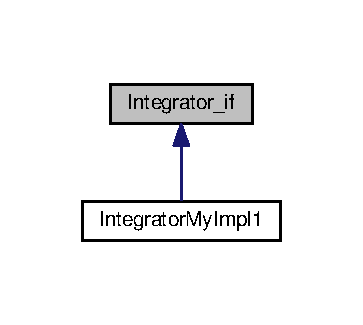
\includegraphics[width=174pt]{class_integrator__if__inherit__graph}
\end{center}
\end{figure}
\subsection*{Public Member Functions}
\begin{DoxyCompactItemize}
\item 
virtual void \hyperlink{class_integrator__if_a49c27818a4b0caf41c39d22a18b41337}{set\-Precision} (double e)=0
\item 
virtual double \hyperlink{class_integrator__if_af3ab4e8ffa96c8970b2e3c980f84e89d}{get\-Precision} ()=0
\item 
virtual double \hyperlink{class_integrator__if_a841c836fd72d4c428178d1e28a999ec9}{integrate} (double min, double max, double($\ast$f)(double, double), double p2)=0
\item 
virtual double \hyperlink{class_integrator__if_a193d992d6101517249d9bee153607aa6}{integrate} (double min, double max, double($\ast$f)(double, double, double), double p2, double p3)=0
\item 
virtual double \hyperlink{class_integrator__if_a306e4fcb840f789d7a918550fa20cc28}{integrate} (double min, double max, double($\ast$f)(double, double, double, double), double p2, double p3, double p4)=0
\item 
virtual double \hyperlink{class_integrator__if_abaeac01142a4da07ba0f07a52732ac79}{integrate} (double min, double max, double($\ast$f)(double, double, double, double, double), double p2, double p3, double p4, double p5)=0
\end{DoxyCompactItemize}


\subsection{Member Function Documentation}
\hypertarget{class_integrator__if_af3ab4e8ffa96c8970b2e3c980f84e89d}{\index{Integrator\-\_\-if@{Integrator\-\_\-if}!get\-Precision@{get\-Precision}}
\index{get\-Precision@{get\-Precision}!Integrator_if@{Integrator\-\_\-if}}
\subsubsection[{get\-Precision}]{\setlength{\rightskip}{0pt plus 5cm}virtual double Integrator\-\_\-if\-::get\-Precision (
\begin{DoxyParamCaption}
{}
\end{DoxyParamCaption}
)\hspace{0.3cm}{\ttfamily [pure virtual]}}}\label{class_integrator__if_af3ab4e8ffa96c8970b2e3c980f84e89d}


Implemented in \hyperlink{class_integrator_my_impl1_aea9d2dd973771048d4468af0ff8ec0d7}{Integrator\-My\-Impl1}.

\hypertarget{class_integrator__if_a841c836fd72d4c428178d1e28a999ec9}{\index{Integrator\-\_\-if@{Integrator\-\_\-if}!integrate@{integrate}}
\index{integrate@{integrate}!Integrator_if@{Integrator\-\_\-if}}
\subsubsection[{integrate}]{\setlength{\rightskip}{0pt plus 5cm}virtual double Integrator\-\_\-if\-::integrate (
\begin{DoxyParamCaption}
\item[{double}]{min, }
\item[{double}]{max, }
\item[{double($\ast$)(double, double)}]{f, }
\item[{double}]{p2}
\end{DoxyParamCaption}
)\hspace{0.3cm}{\ttfamily [pure virtual]}}}\label{class_integrator__if_a841c836fd72d4c428178d1e28a999ec9}


Implemented in \hyperlink{class_integrator_my_impl1_a0f5f36cb45c4d50832b1d9bc8bdfcf8b}{Integrator\-My\-Impl1}.

\hypertarget{class_integrator__if_a193d992d6101517249d9bee153607aa6}{\index{Integrator\-\_\-if@{Integrator\-\_\-if}!integrate@{integrate}}
\index{integrate@{integrate}!Integrator_if@{Integrator\-\_\-if}}
\subsubsection[{integrate}]{\setlength{\rightskip}{0pt plus 5cm}virtual double Integrator\-\_\-if\-::integrate (
\begin{DoxyParamCaption}
\item[{double}]{min, }
\item[{double}]{max, }
\item[{double($\ast$)(double, double, double)}]{f, }
\item[{double}]{p2, }
\item[{double}]{p3}
\end{DoxyParamCaption}
)\hspace{0.3cm}{\ttfamily [pure virtual]}}}\label{class_integrator__if_a193d992d6101517249d9bee153607aa6}


Implemented in \hyperlink{class_integrator_my_impl1_a841ac12407f9c2941d37e753c3916236}{Integrator\-My\-Impl1}.

\hypertarget{class_integrator__if_a306e4fcb840f789d7a918550fa20cc28}{\index{Integrator\-\_\-if@{Integrator\-\_\-if}!integrate@{integrate}}
\index{integrate@{integrate}!Integrator_if@{Integrator\-\_\-if}}
\subsubsection[{integrate}]{\setlength{\rightskip}{0pt plus 5cm}virtual double Integrator\-\_\-if\-::integrate (
\begin{DoxyParamCaption}
\item[{double}]{min, }
\item[{double}]{max, }
\item[{double($\ast$)(double, double, double, double)}]{f, }
\item[{double}]{p2, }
\item[{double}]{p3, }
\item[{double}]{p4}
\end{DoxyParamCaption}
)\hspace{0.3cm}{\ttfamily [pure virtual]}}}\label{class_integrator__if_a306e4fcb840f789d7a918550fa20cc28}


Implemented in \hyperlink{class_integrator_my_impl1_a9bf5693a1c2eff13b04a54771bd4c9df}{Integrator\-My\-Impl1}.

\hypertarget{class_integrator__if_abaeac01142a4da07ba0f07a52732ac79}{\index{Integrator\-\_\-if@{Integrator\-\_\-if}!integrate@{integrate}}
\index{integrate@{integrate}!Integrator_if@{Integrator\-\_\-if}}
\subsubsection[{integrate}]{\setlength{\rightskip}{0pt plus 5cm}virtual double Integrator\-\_\-if\-::integrate (
\begin{DoxyParamCaption}
\item[{double}]{min, }
\item[{double}]{max, }
\item[{double($\ast$)(double, double, double, double, double)}]{f, }
\item[{double}]{p2, }
\item[{double}]{p3, }
\item[{double}]{p4, }
\item[{double}]{p5}
\end{DoxyParamCaption}
)\hspace{0.3cm}{\ttfamily [pure virtual]}}}\label{class_integrator__if_abaeac01142a4da07ba0f07a52732ac79}


Implemented in \hyperlink{class_integrator_my_impl1_a5cff324672903d41acb47f852d1a5918}{Integrator\-My\-Impl1}.

\hypertarget{class_integrator__if_a49c27818a4b0caf41c39d22a18b41337}{\index{Integrator\-\_\-if@{Integrator\-\_\-if}!set\-Precision@{set\-Precision}}
\index{set\-Precision@{set\-Precision}!Integrator_if@{Integrator\-\_\-if}}
\subsubsection[{set\-Precision}]{\setlength{\rightskip}{0pt plus 5cm}virtual void Integrator\-\_\-if\-::set\-Precision (
\begin{DoxyParamCaption}
\item[{double}]{e}
\end{DoxyParamCaption}
)\hspace{0.3cm}{\ttfamily [pure virtual]}}}\label{class_integrator__if_a49c27818a4b0caf41c39d22a18b41337}


Implemented in \hyperlink{class_integrator_my_impl1_a74ca07f81a587332dab9aee756063c43}{Integrator\-My\-Impl1}.



The documentation for this class was generated from the following file\-:\begin{DoxyCompactItemize}
\item 
\hyperlink{_integrator__if_8h}{Integrator\-\_\-if.\-h}\end{DoxyCompactItemize}

\hypertarget{class_integrator_my_impl1}{\section{Integrator\-My\-Impl1 Class Reference}
\label{class_integrator_my_impl1}\index{Integrator\-My\-Impl1@{Integrator\-My\-Impl1}}
}


{\ttfamily \#include $<$Integrator\-My\-Impl1.\-h$>$}



Inheritance diagram for Integrator\-My\-Impl1\-:\nopagebreak
\begin{figure}[H]
\begin{center}
\leavevmode
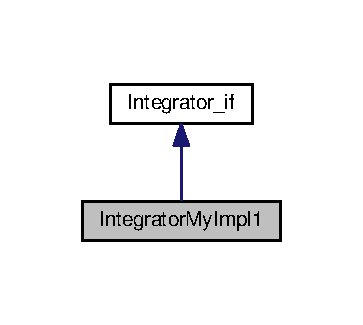
\includegraphics[width=174pt]{class_integrator_my_impl1__inherit__graph}
\end{center}
\end{figure}


Collaboration diagram for Integrator\-My\-Impl1\-:\nopagebreak
\begin{figure}[H]
\begin{center}
\leavevmode
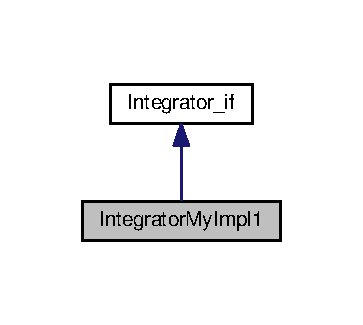
\includegraphics[width=174pt]{class_integrator_my_impl1__coll__graph}
\end{center}
\end{figure}
\subsection*{Public Member Functions}
\begin{DoxyCompactItemize}
\item 
\hyperlink{class_integrator_my_impl1_a1d1b8df78549b530f99b88d6a83e85b0}{Integrator\-My\-Impl1} ()
\item 
\hyperlink{class_integrator_my_impl1_a1cf39ec6d11720cc9965a0b04495080b}{Integrator\-My\-Impl1} (const \hyperlink{class_integrator_my_impl1}{Integrator\-My\-Impl1} \&orig)
\item 
\hyperlink{class_integrator_my_impl1_a483165ecb54e8cf6c43e2972f0ab07b4}{$\sim$\-Integrator\-My\-Impl1} ()
\item 
void \hyperlink{class_integrator_my_impl1_a74ca07f81a587332dab9aee756063c43}{set\-Precision} (double e)
\item 
double \hyperlink{class_integrator_my_impl1_aea9d2dd973771048d4468af0ff8ec0d7}{get\-Precision} ()
\item 
double \hyperlink{class_integrator_my_impl1_a0f5f36cb45c4d50832b1d9bc8bdfcf8b}{integrate} (double min, double max, double($\ast$f)(double, double), double p2)
\item 
double \hyperlink{class_integrator_my_impl1_a841ac12407f9c2941d37e753c3916236}{integrate} (double min, double max, double($\ast$f)(double, double, double), double p2, double p3)
\item 
double \hyperlink{class_integrator_my_impl1_a9bf5693a1c2eff13b04a54771bd4c9df}{integrate} (double min, double max, double($\ast$f)(double, double, double, double), double p2, double p3, double p4)
\item 
double \hyperlink{class_integrator_my_impl1_a5cff324672903d41acb47f852d1a5918}{integrate} (double min, double max, double($\ast$f)(double, double, double, double, double), double p2, double p3, double p4, double p5)
\end{DoxyCompactItemize}


\subsection{Constructor \& Destructor Documentation}
\hypertarget{class_integrator_my_impl1_a1d1b8df78549b530f99b88d6a83e85b0}{\index{Integrator\-My\-Impl1@{Integrator\-My\-Impl1}!Integrator\-My\-Impl1@{Integrator\-My\-Impl1}}
\index{Integrator\-My\-Impl1@{Integrator\-My\-Impl1}!IntegratorMyImpl1@{Integrator\-My\-Impl1}}
\subsubsection[{Integrator\-My\-Impl1}]{\setlength{\rightskip}{0pt plus 5cm}Integrator\-My\-Impl1\-::\-Integrator\-My\-Impl1 (
\begin{DoxyParamCaption}
{}
\end{DoxyParamCaption}
)}}\label{class_integrator_my_impl1_a1d1b8df78549b530f99b88d6a83e85b0}
\hypertarget{class_integrator_my_impl1_a1cf39ec6d11720cc9965a0b04495080b}{\index{Integrator\-My\-Impl1@{Integrator\-My\-Impl1}!Integrator\-My\-Impl1@{Integrator\-My\-Impl1}}
\index{Integrator\-My\-Impl1@{Integrator\-My\-Impl1}!IntegratorMyImpl1@{Integrator\-My\-Impl1}}
\subsubsection[{Integrator\-My\-Impl1}]{\setlength{\rightskip}{0pt plus 5cm}Integrator\-My\-Impl1\-::\-Integrator\-My\-Impl1 (
\begin{DoxyParamCaption}
\item[{const {\bf Integrator\-My\-Impl1} \&}]{orig}
\end{DoxyParamCaption}
)}}\label{class_integrator_my_impl1_a1cf39ec6d11720cc9965a0b04495080b}
\hypertarget{class_integrator_my_impl1_a483165ecb54e8cf6c43e2972f0ab07b4}{\index{Integrator\-My\-Impl1@{Integrator\-My\-Impl1}!$\sim$\-Integrator\-My\-Impl1@{$\sim$\-Integrator\-My\-Impl1}}
\index{$\sim$\-Integrator\-My\-Impl1@{$\sim$\-Integrator\-My\-Impl1}!IntegratorMyImpl1@{Integrator\-My\-Impl1}}
\subsubsection[{$\sim$\-Integrator\-My\-Impl1}]{\setlength{\rightskip}{0pt plus 5cm}Integrator\-My\-Impl1\-::$\sim$\-Integrator\-My\-Impl1 (
\begin{DoxyParamCaption}
{}
\end{DoxyParamCaption}
)}}\label{class_integrator_my_impl1_a483165ecb54e8cf6c43e2972f0ab07b4}


\subsection{Member Function Documentation}
\hypertarget{class_integrator_my_impl1_aea9d2dd973771048d4468af0ff8ec0d7}{\index{Integrator\-My\-Impl1@{Integrator\-My\-Impl1}!get\-Precision@{get\-Precision}}
\index{get\-Precision@{get\-Precision}!IntegratorMyImpl1@{Integrator\-My\-Impl1}}
\subsubsection[{get\-Precision}]{\setlength{\rightskip}{0pt plus 5cm}double Integrator\-My\-Impl1\-::get\-Precision (
\begin{DoxyParamCaption}
{}
\end{DoxyParamCaption}
)\hspace{0.3cm}{\ttfamily [virtual]}}}\label{class_integrator_my_impl1_aea9d2dd973771048d4468af0ff8ec0d7}


Implements \hyperlink{class_integrator__if_af3ab4e8ffa96c8970b2e3c980f84e89d}{Integrator\-\_\-if}.

\hypertarget{class_integrator_my_impl1_a0f5f36cb45c4d50832b1d9bc8bdfcf8b}{\index{Integrator\-My\-Impl1@{Integrator\-My\-Impl1}!integrate@{integrate}}
\index{integrate@{integrate}!IntegratorMyImpl1@{Integrator\-My\-Impl1}}
\subsubsection[{integrate}]{\setlength{\rightskip}{0pt plus 5cm}double Integrator\-My\-Impl1\-::integrate (
\begin{DoxyParamCaption}
\item[{double}]{min, }
\item[{double}]{max, }
\item[{double($\ast$)(double, double)}]{f, }
\item[{double}]{p2}
\end{DoxyParamCaption}
)\hspace{0.3cm}{\ttfamily [virtual]}}}\label{class_integrator_my_impl1_a0f5f36cb45c4d50832b1d9bc8bdfcf8b}


Implements \hyperlink{class_integrator__if_a841c836fd72d4c428178d1e28a999ec9}{Integrator\-\_\-if}.

\hypertarget{class_integrator_my_impl1_a841ac12407f9c2941d37e753c3916236}{\index{Integrator\-My\-Impl1@{Integrator\-My\-Impl1}!integrate@{integrate}}
\index{integrate@{integrate}!IntegratorMyImpl1@{Integrator\-My\-Impl1}}
\subsubsection[{integrate}]{\setlength{\rightskip}{0pt plus 5cm}double Integrator\-My\-Impl1\-::integrate (
\begin{DoxyParamCaption}
\item[{double}]{min, }
\item[{double}]{max, }
\item[{double($\ast$)(double, double, double)}]{f, }
\item[{double}]{p2, }
\item[{double}]{p3}
\end{DoxyParamCaption}
)\hspace{0.3cm}{\ttfamily [virtual]}}}\label{class_integrator_my_impl1_a841ac12407f9c2941d37e753c3916236}


Implements \hyperlink{class_integrator__if_a193d992d6101517249d9bee153607aa6}{Integrator\-\_\-if}.

\hypertarget{class_integrator_my_impl1_a9bf5693a1c2eff13b04a54771bd4c9df}{\index{Integrator\-My\-Impl1@{Integrator\-My\-Impl1}!integrate@{integrate}}
\index{integrate@{integrate}!IntegratorMyImpl1@{Integrator\-My\-Impl1}}
\subsubsection[{integrate}]{\setlength{\rightskip}{0pt plus 5cm}double Integrator\-My\-Impl1\-::integrate (
\begin{DoxyParamCaption}
\item[{double}]{min, }
\item[{double}]{max, }
\item[{double($\ast$)(double, double, double, double)}]{f, }
\item[{double}]{p2, }
\item[{double}]{p3, }
\item[{double}]{p4}
\end{DoxyParamCaption}
)\hspace{0.3cm}{\ttfamily [virtual]}}}\label{class_integrator_my_impl1_a9bf5693a1c2eff13b04a54771bd4c9df}


Implements \hyperlink{class_integrator__if_a306e4fcb840f789d7a918550fa20cc28}{Integrator\-\_\-if}.

\hypertarget{class_integrator_my_impl1_a5cff324672903d41acb47f852d1a5918}{\index{Integrator\-My\-Impl1@{Integrator\-My\-Impl1}!integrate@{integrate}}
\index{integrate@{integrate}!IntegratorMyImpl1@{Integrator\-My\-Impl1}}
\subsubsection[{integrate}]{\setlength{\rightskip}{0pt plus 5cm}double Integrator\-My\-Impl1\-::integrate (
\begin{DoxyParamCaption}
\item[{double}]{min, }
\item[{double}]{max, }
\item[{double($\ast$)(double, double, double, double, double)}]{f, }
\item[{double}]{p2, }
\item[{double}]{p3, }
\item[{double}]{p4, }
\item[{double}]{p5}
\end{DoxyParamCaption}
)\hspace{0.3cm}{\ttfamily [virtual]}}}\label{class_integrator_my_impl1_a5cff324672903d41acb47f852d1a5918}


Implements \hyperlink{class_integrator__if_abaeac01142a4da07ba0f07a52732ac79}{Integrator\-\_\-if}.

\hypertarget{class_integrator_my_impl1_a74ca07f81a587332dab9aee756063c43}{\index{Integrator\-My\-Impl1@{Integrator\-My\-Impl1}!set\-Precision@{set\-Precision}}
\index{set\-Precision@{set\-Precision}!IntegratorMyImpl1@{Integrator\-My\-Impl1}}
\subsubsection[{set\-Precision}]{\setlength{\rightskip}{0pt plus 5cm}void Integrator\-My\-Impl1\-::set\-Precision (
\begin{DoxyParamCaption}
\item[{double}]{e}
\end{DoxyParamCaption}
)\hspace{0.3cm}{\ttfamily [virtual]}}}\label{class_integrator_my_impl1_a74ca07f81a587332dab9aee756063c43}


Implements \hyperlink{class_integrator__if_a49c27818a4b0caf41c39d22a18b41337}{Integrator\-\_\-if}.



The documentation for this class was generated from the following files\-:\begin{DoxyCompactItemize}
\item 
\hyperlink{_integrator_my_impl1_8h}{Integrator\-My\-Impl1.\-h}\item 
\hyperlink{_integrator_my_impl1_8cpp}{Integrator\-My\-Impl1.\-cpp}\end{DoxyCompactItemize}

\hypertarget{class_linked_by}{\section{Linked\-By Class Reference}
\label{class_linked_by}\index{Linked\-By@{Linked\-By}}
}


{\ttfamily \#include $<$Linked\-By.\-h$>$}



Inheritance diagram for Linked\-By\-:\nopagebreak
\begin{figure}[H]
\begin{center}
\leavevmode
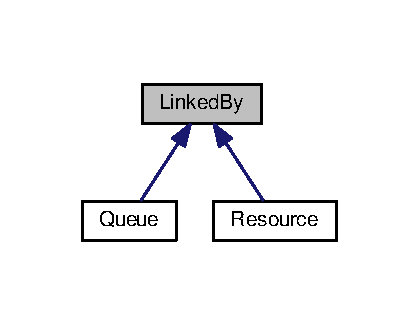
\includegraphics[width=201pt]{class_linked_by__inherit__graph}
\end{center}
\end{figure}
\subsection*{Public Member Functions}
\begin{DoxyCompactItemize}
\item 
\hyperlink{class_linked_by_af786842e7d3f98fe43067114dc777b8b}{Linked\-By} ()
\item 
\hyperlink{class_linked_by_ace412273cc6d87ffab7da022c2ae0d65}{Linked\-By} (const \hyperlink{class_linked_by}{Linked\-By} \&orig)
\item 
virtual \hyperlink{class_linked_by_af5c2ee380dcad914ac10cf4132e4a7ae}{$\sim$\-Linked\-By} ()
\item 
void \hyperlink{class_linked_by_afbfa186e0511d6ce2efdb58c89d834c9}{add\-Link} ()
\item 
void \hyperlink{class_linked_by_a2cd33b134ec4bf9043d0bf7e7d4d8f25}{remove\-Link} ()
\item 
bool \hyperlink{class_linked_by_a5f1cd64ec1f6eb15f06d3332071d82b7}{is\-Linked} ()
\end{DoxyCompactItemize}


\subsection{Constructor \& Destructor Documentation}
\hypertarget{class_linked_by_af786842e7d3f98fe43067114dc777b8b}{\index{Linked\-By@{Linked\-By}!Linked\-By@{Linked\-By}}
\index{Linked\-By@{Linked\-By}!LinkedBy@{Linked\-By}}
\subsubsection[{Linked\-By}]{\setlength{\rightskip}{0pt plus 5cm}Linked\-By\-::\-Linked\-By (
\begin{DoxyParamCaption}
{}
\end{DoxyParamCaption}
)}}\label{class_linked_by_af786842e7d3f98fe43067114dc777b8b}
\hypertarget{class_linked_by_ace412273cc6d87ffab7da022c2ae0d65}{\index{Linked\-By@{Linked\-By}!Linked\-By@{Linked\-By}}
\index{Linked\-By@{Linked\-By}!LinkedBy@{Linked\-By}}
\subsubsection[{Linked\-By}]{\setlength{\rightskip}{0pt plus 5cm}Linked\-By\-::\-Linked\-By (
\begin{DoxyParamCaption}
\item[{const {\bf Linked\-By} \&}]{orig}
\end{DoxyParamCaption}
)}}\label{class_linked_by_ace412273cc6d87ffab7da022c2ae0d65}
\hypertarget{class_linked_by_af5c2ee380dcad914ac10cf4132e4a7ae}{\index{Linked\-By@{Linked\-By}!$\sim$\-Linked\-By@{$\sim$\-Linked\-By}}
\index{$\sim$\-Linked\-By@{$\sim$\-Linked\-By}!LinkedBy@{Linked\-By}}
\subsubsection[{$\sim$\-Linked\-By}]{\setlength{\rightskip}{0pt plus 5cm}Linked\-By\-::$\sim$\-Linked\-By (
\begin{DoxyParamCaption}
{}
\end{DoxyParamCaption}
)\hspace{0.3cm}{\ttfamily [virtual]}}}\label{class_linked_by_af5c2ee380dcad914ac10cf4132e4a7ae}


\subsection{Member Function Documentation}
\hypertarget{class_linked_by_afbfa186e0511d6ce2efdb58c89d834c9}{\index{Linked\-By@{Linked\-By}!add\-Link@{add\-Link}}
\index{add\-Link@{add\-Link}!LinkedBy@{Linked\-By}}
\subsubsection[{add\-Link}]{\setlength{\rightskip}{0pt plus 5cm}void Linked\-By\-::add\-Link (
\begin{DoxyParamCaption}
{}
\end{DoxyParamCaption}
)}}\label{class_linked_by_afbfa186e0511d6ce2efdb58c89d834c9}
\hypertarget{class_linked_by_a5f1cd64ec1f6eb15f06d3332071d82b7}{\index{Linked\-By@{Linked\-By}!is\-Linked@{is\-Linked}}
\index{is\-Linked@{is\-Linked}!LinkedBy@{Linked\-By}}
\subsubsection[{is\-Linked}]{\setlength{\rightskip}{0pt plus 5cm}bool Linked\-By\-::is\-Linked (
\begin{DoxyParamCaption}
{}
\end{DoxyParamCaption}
)}}\label{class_linked_by_a5f1cd64ec1f6eb15f06d3332071d82b7}
\hypertarget{class_linked_by_a2cd33b134ec4bf9043d0bf7e7d4d8f25}{\index{Linked\-By@{Linked\-By}!remove\-Link@{remove\-Link}}
\index{remove\-Link@{remove\-Link}!LinkedBy@{Linked\-By}}
\subsubsection[{remove\-Link}]{\setlength{\rightskip}{0pt plus 5cm}void Linked\-By\-::remove\-Link (
\begin{DoxyParamCaption}
{}
\end{DoxyParamCaption}
)}}\label{class_linked_by_a2cd33b134ec4bf9043d0bf7e7d4d8f25}


The documentation for this class was generated from the following files\-:\begin{DoxyCompactItemize}
\item 
\hyperlink{_linked_by_8h}{Linked\-By.\-h}\item 
\hyperlink{_linked_by_8cpp}{Linked\-By.\-cpp}\end{DoxyCompactItemize}

\hypertarget{class_list}{\section{List$<$ T $>$ Class Template Reference}
\label{class_list}\index{List$<$ T $>$@{List$<$ T $>$}}
}


{\ttfamily \#include $<$List.\-h$>$}

\subsection*{Public Types}
\begin{DoxyCompactItemize}
\item 
using \hyperlink{class_list_ae43380038701ec3a2fbecaf31f37dd19}{Comp\-Funct} = std\-::function$<$ bool(const T, const T)$>$
\end{DoxyCompactItemize}
\subsection*{Public Member Functions}
\begin{DoxyCompactItemize}
\item 
\hyperlink{class_list_a5c5e27671b21b3815d4e25b953c69454}{List} ()
\item 
\hyperlink{class_list_a46e402e625d805b8ccb565129d4d9680}{List} (const \hyperlink{class_list}{List} \&orig)
\item 
virtual \hyperlink{class_list_a2b58189090f6e5ce52939c9195e59e85}{$\sim$\-List} ()
\item 
unsigned int \hyperlink{class_list_ad908ab5cf19370fcdf61cf1927e5e8f5}{size} ()
\item 
bool \hyperlink{class_list_a3737ca60365287ce663393d8c07d1a41}{empty} ()
\item 
void \hyperlink{class_list_ae296516a252e11963dbf963727ce429a}{clear} ()
\item 
void \hyperlink{class_list_a024af4543f71544345351a45850c42d8}{pop\-\_\-front} ()
\item 
{\footnotesize template$<$class Compare $>$ }\\void \hyperlink{class_list_af5bf0ad4812b1a9da9eb20a4646e3e96}{sort} (Compare comp)
\item 
std\-::list$<$ T $>$ $\ast$ \hyperlink{class_list_a570498345450f635b72d1ca2675145cc}{get\-List} () const 
\item 
T \hyperlink{class_list_a3439065c3222c241427e9deb6adf1b01}{create} ()
\item 
{\footnotesize template$<$typename U $>$ }\\T \hyperlink{class_list_a767b6b53a19368f4623d72cea74f9c7b}{create} (U arg)
\item 
std\-::string \hyperlink{class_list_a8f30a708a550bcca33f64dc6fea8affa}{show} ()
\item 
std\-::list$<$ T $>$\-::iterator \hyperlink{class_list_a2f50d3342e016ec57876798ad4e8bf31}{find} (T element)
\item 
void \hyperlink{class_list_a518d00fd77740525522949d4316e8826}{insert} (T element)
\item 
void \hyperlink{class_list_a0ac08f7f3dad900b99e9a73e76d2beee}{remove} (T element)
\item 
T \hyperlink{class_list_a2dce655743c2b6c7cc7c9b6034badf78}{next} ()
\item 
T \hyperlink{class_list_a42761114ff6730da1402089d4bd3f795}{first} ()
\item 
T \hyperlink{class_list_a9944c09ee1bd6390bbf017be5c858063}{last} ()
\item 
T \hyperlink{class_list_ab43f87321c901694807e6c9315a72cd0}{previous} ()
\item 
T \hyperlink{class_list_a58474bac3aa3d1ef7208aa06a3789d57}{actual} ()
\item 
void \hyperlink{class_list_a31a37746c0d960f2f2bb4071b2735c5e}{set\-Sort\-Func} (\hyperlink{class_list_ae43380038701ec3a2fbecaf31f37dd19}{Comp\-Funct} \-\_\-sort\-Func)
\end{DoxyCompactItemize}


\subsection{Member Typedef Documentation}
\hypertarget{class_list_ae43380038701ec3a2fbecaf31f37dd19}{\index{List@{List}!Comp\-Funct@{Comp\-Funct}}
\index{Comp\-Funct@{Comp\-Funct}!List@{List}}
\subsubsection[{Comp\-Funct}]{\setlength{\rightskip}{0pt plus 5cm}template$<$typename T$>$ using {\bf List}$<$ T $>$\-::{\bf Comp\-Funct} =  std\-::function$<$bool(const T, const T)$>$}}\label{class_list_ae43380038701ec3a2fbecaf31f37dd19}


\subsection{Constructor \& Destructor Documentation}
\hypertarget{class_list_a5c5e27671b21b3815d4e25b953c69454}{\index{List@{List}!List@{List}}
\index{List@{List}!List@{List}}
\subsubsection[{List}]{\setlength{\rightskip}{0pt plus 5cm}template$<$typename T $>$ {\bf List}$<$ T $>$\-::{\bf List} (
\begin{DoxyParamCaption}
{}
\end{DoxyParamCaption}
)}}\label{class_list_a5c5e27671b21b3815d4e25b953c69454}
\hypertarget{class_list_a46e402e625d805b8ccb565129d4d9680}{\index{List@{List}!List@{List}}
\index{List@{List}!List@{List}}
\subsubsection[{List}]{\setlength{\rightskip}{0pt plus 5cm}template$<$typename T $>$ {\bf List}$<$ T $>$\-::{\bf List} (
\begin{DoxyParamCaption}
\item[{const {\bf List}$<$ T $>$ \&}]{orig}
\end{DoxyParamCaption}
)}}\label{class_list_a46e402e625d805b8ccb565129d4d9680}
\hypertarget{class_list_a2b58189090f6e5ce52939c9195e59e85}{\index{List@{List}!$\sim$\-List@{$\sim$\-List}}
\index{$\sim$\-List@{$\sim$\-List}!List@{List}}
\subsubsection[{$\sim$\-List}]{\setlength{\rightskip}{0pt plus 5cm}template$<$typename T $>$ {\bf List}$<$ T $>$\-::$\sim${\bf List} (
\begin{DoxyParamCaption}
{}
\end{DoxyParamCaption}
)\hspace{0.3cm}{\ttfamily [virtual]}}}\label{class_list_a2b58189090f6e5ce52939c9195e59e85}


\subsection{Member Function Documentation}
\hypertarget{class_list_a58474bac3aa3d1ef7208aa06a3789d57}{\index{List@{List}!actual@{actual}}
\index{actual@{actual}!List@{List}}
\subsubsection[{actual}]{\setlength{\rightskip}{0pt plus 5cm}template$<$typename T $>$ T {\bf List}$<$ T $>$\-::actual (
\begin{DoxyParamCaption}
{}
\end{DoxyParamCaption}
)}}\label{class_list_a58474bac3aa3d1ef7208aa06a3789d57}
\hypertarget{class_list_ae296516a252e11963dbf963727ce429a}{\index{List@{List}!clear@{clear}}
\index{clear@{clear}!List@{List}}
\subsubsection[{clear}]{\setlength{\rightskip}{0pt plus 5cm}template$<$typename T $>$ void {\bf List}$<$ T $>$\-::clear (
\begin{DoxyParamCaption}
{}
\end{DoxyParamCaption}
)}}\label{class_list_ae296516a252e11963dbf963727ce429a}
\hypertarget{class_list_a3439065c3222c241427e9deb6adf1b01}{\index{List@{List}!create@{create}}
\index{create@{create}!List@{List}}
\subsubsection[{create}]{\setlength{\rightskip}{0pt plus 5cm}template$<$typename T $>$ T {\bf List}$<$ T $>$\-::create (
\begin{DoxyParamCaption}
{}
\end{DoxyParamCaption}
)}}\label{class_list_a3439065c3222c241427e9deb6adf1b01}
\hypertarget{class_list_a767b6b53a19368f4623d72cea74f9c7b}{\index{List@{List}!create@{create}}
\index{create@{create}!List@{List}}
\subsubsection[{create}]{\setlength{\rightskip}{0pt plus 5cm}template$<$typename T $>$ template$<$typename U $>$ T {\bf List}$<$ T $>$\-::create (
\begin{DoxyParamCaption}
\item[{U}]{arg}
\end{DoxyParamCaption}
)}}\label{class_list_a767b6b53a19368f4623d72cea74f9c7b}
\hypertarget{class_list_a3737ca60365287ce663393d8c07d1a41}{\index{List@{List}!empty@{empty}}
\index{empty@{empty}!List@{List}}
\subsubsection[{empty}]{\setlength{\rightskip}{0pt plus 5cm}template$<$typename T $>$ bool {\bf List}$<$ T $>$\-::empty (
\begin{DoxyParamCaption}
{}
\end{DoxyParamCaption}
)}}\label{class_list_a3737ca60365287ce663393d8c07d1a41}
\hypertarget{class_list_a2f50d3342e016ec57876798ad4e8bf31}{\index{List@{List}!find@{find}}
\index{find@{find}!List@{List}}
\subsubsection[{find}]{\setlength{\rightskip}{0pt plus 5cm}template$<$typename T$>$ std\-::list$<$ T $>$\-::iterator {\bf List}$<$ T $>$\-::find (
\begin{DoxyParamCaption}
\item[{T}]{element}
\end{DoxyParamCaption}
)}}\label{class_list_a2f50d3342e016ec57876798ad4e8bf31}
\hypertarget{class_list_a42761114ff6730da1402089d4bd3f795}{\index{List@{List}!first@{first}}
\index{first@{first}!List@{List}}
\subsubsection[{first}]{\setlength{\rightskip}{0pt plus 5cm}template$<$typename T $>$ T {\bf List}$<$ T $>$\-::first (
\begin{DoxyParamCaption}
{}
\end{DoxyParamCaption}
)}}\label{class_list_a42761114ff6730da1402089d4bd3f795}
\hypertarget{class_list_a570498345450f635b72d1ca2675145cc}{\index{List@{List}!get\-List@{get\-List}}
\index{get\-List@{get\-List}!List@{List}}
\subsubsection[{get\-List}]{\setlength{\rightskip}{0pt plus 5cm}template$<$typename T $>$ std\-::list$<$ T $>$ $\ast$ {\bf List}$<$ T $>$\-::get\-List (
\begin{DoxyParamCaption}
{}
\end{DoxyParamCaption}
) const}}\label{class_list_a570498345450f635b72d1ca2675145cc}
\hypertarget{class_list_a518d00fd77740525522949d4316e8826}{\index{List@{List}!insert@{insert}}
\index{insert@{insert}!List@{List}}
\subsubsection[{insert}]{\setlength{\rightskip}{0pt plus 5cm}template$<$typename T$>$ void {\bf List}$<$ T $>$\-::insert (
\begin{DoxyParamCaption}
\item[{T}]{element}
\end{DoxyParamCaption}
)}}\label{class_list_a518d00fd77740525522949d4316e8826}
\hypertarget{class_list_a9944c09ee1bd6390bbf017be5c858063}{\index{List@{List}!last@{last}}
\index{last@{last}!List@{List}}
\subsubsection[{last}]{\setlength{\rightskip}{0pt plus 5cm}template$<$typename T $>$ T {\bf List}$<$ T $>$\-::last (
\begin{DoxyParamCaption}
{}
\end{DoxyParamCaption}
)}}\label{class_list_a9944c09ee1bd6390bbf017be5c858063}
\hypertarget{class_list_a2dce655743c2b6c7cc7c9b6034badf78}{\index{List@{List}!next@{next}}
\index{next@{next}!List@{List}}
\subsubsection[{next}]{\setlength{\rightskip}{0pt plus 5cm}template$<$typename T $>$ T {\bf List}$<$ T $>$\-::next (
\begin{DoxyParamCaption}
{}
\end{DoxyParamCaption}
)}}\label{class_list_a2dce655743c2b6c7cc7c9b6034badf78}
\hypertarget{class_list_a024af4543f71544345351a45850c42d8}{\index{List@{List}!pop\-\_\-front@{pop\-\_\-front}}
\index{pop\-\_\-front@{pop\-\_\-front}!List@{List}}
\subsubsection[{pop\-\_\-front}]{\setlength{\rightskip}{0pt plus 5cm}template$<$typename T $>$ void {\bf List}$<$ T $>$\-::pop\-\_\-front (
\begin{DoxyParamCaption}
{}
\end{DoxyParamCaption}
)}}\label{class_list_a024af4543f71544345351a45850c42d8}
\hypertarget{class_list_ab43f87321c901694807e6c9315a72cd0}{\index{List@{List}!previous@{previous}}
\index{previous@{previous}!List@{List}}
\subsubsection[{previous}]{\setlength{\rightskip}{0pt plus 5cm}template$<$typename T $>$ T {\bf List}$<$ T $>$\-::previous (
\begin{DoxyParamCaption}
{}
\end{DoxyParamCaption}
)}}\label{class_list_ab43f87321c901694807e6c9315a72cd0}
\hypertarget{class_list_a0ac08f7f3dad900b99e9a73e76d2beee}{\index{List@{List}!remove@{remove}}
\index{remove@{remove}!List@{List}}
\subsubsection[{remove}]{\setlength{\rightskip}{0pt plus 5cm}template$<$typename T$>$ void {\bf List}$<$ T $>$\-::remove (
\begin{DoxyParamCaption}
\item[{T}]{element}
\end{DoxyParamCaption}
)}}\label{class_list_a0ac08f7f3dad900b99e9a73e76d2beee}
\hypertarget{class_list_a31a37746c0d960f2f2bb4071b2735c5e}{\index{List@{List}!set\-Sort\-Func@{set\-Sort\-Func}}
\index{set\-Sort\-Func@{set\-Sort\-Func}!List@{List}}
\subsubsection[{set\-Sort\-Func}]{\setlength{\rightskip}{0pt plus 5cm}template$<$typename T $>$ void {\bf List}$<$ T $>$\-::set\-Sort\-Func (
\begin{DoxyParamCaption}
\item[{{\bf Comp\-Funct}}]{\-\_\-sort\-Func}
\end{DoxyParamCaption}
)}}\label{class_list_a31a37746c0d960f2f2bb4071b2735c5e}
\hypertarget{class_list_a8f30a708a550bcca33f64dc6fea8affa}{\index{List@{List}!show@{show}}
\index{show@{show}!List@{List}}
\subsubsection[{show}]{\setlength{\rightskip}{0pt plus 5cm}template$<$typename T $>$ std\-::string {\bf List}$<$ T $>$\-::show (
\begin{DoxyParamCaption}
{}
\end{DoxyParamCaption}
)}}\label{class_list_a8f30a708a550bcca33f64dc6fea8affa}
\hypertarget{class_list_ad908ab5cf19370fcdf61cf1927e5e8f5}{\index{List@{List}!size@{size}}
\index{size@{size}!List@{List}}
\subsubsection[{size}]{\setlength{\rightskip}{0pt plus 5cm}template$<$typename T $>$ unsigned int {\bf List}$<$ T $>$\-::size (
\begin{DoxyParamCaption}
{}
\end{DoxyParamCaption}
)}}\label{class_list_ad908ab5cf19370fcdf61cf1927e5e8f5}
\hypertarget{class_list_af5bf0ad4812b1a9da9eb20a4646e3e96}{\index{List@{List}!sort@{sort}}
\index{sort@{sort}!List@{List}}
\subsubsection[{sort}]{\setlength{\rightskip}{0pt plus 5cm}template$<$typename T $>$ template$<$class Compare $>$ void {\bf List}$<$ T $>$\-::sort (
\begin{DoxyParamCaption}
\item[{Compare}]{comp}
\end{DoxyParamCaption}
)}}\label{class_list_af5bf0ad4812b1a9da9eb20a4646e3e96}


The documentation for this class was generated from the following file\-:\begin{DoxyCompactItemize}
\item 
\hyperlink{_list_8h}{List.\-h}\end{DoxyCompactItemize}

\hypertarget{class_model}{\section{Model Class Reference}
\label{class_model}\index{Model@{Model}}
}


{\ttfamily \#include $<$Model.\-h$>$}

\subsection*{Public Member Functions}
\begin{DoxyCompactItemize}
\item 
\hyperlink{class_model_ae86e1403523e8036ba6366d1967ecac0}{Model} (\hyperlink{class_simulator}{Simulator} $\ast$simulator)
\item 
\hyperlink{class_model_afdedf278781f785abeecf5f450e43653}{Model} (const \hyperlink{class_model}{Model} \&orig)
\item 
virtual \hyperlink{class_model_ad6ebd2062a0b823db841a0b88baac4c0}{$\sim$\-Model} ()
\item 
void \hyperlink{class_model_a6fd6613a5141552a6493eb3a840cde24}{start\-Simulation} ()
\item 
void \hyperlink{class_model_ab10d4bdc433d11bf4bb7117675091d8c}{pause\-Simulation} ()
\item 
void \hyperlink{class_model_a025b6ab3112a1df6f7773389b096302c}{step\-Simulation} ()
\item 
void \hyperlink{class_model_a6452e846a5e560220236b7a59f1dd84b}{stop\-Simulation} ()
\item 
void \hyperlink{class_model_a8be70da19c6c315269acc5a3fd2e3b7d}{restart\-Simulation} ()
\item 
void \hyperlink{class_model_a44c66f552308e7a6a5701801186a8637}{show\-Reports} ()
\item 
void \hyperlink{class_model_a99238439363a292fe1fc503eb2157a55}{set\-Pause\-On\-Event} (bool \-\_\-pause\-On\-Event)
\item 
bool \hyperlink{class_model_a1dda07db7bddff456907067eeeb5c21a}{is\-Pause\-On\-Event} () const 
\item 
bool \hyperlink{class_model_ae099910781f5267a51fb5d607246af4a}{save\-Model} (std\-::string filename)
\item 
bool \hyperlink{class_model_aba57e8b62d4dcc3ac8e3037933fa6f04}{load\-Model} (std\-::string filename)
\item 
bool \hyperlink{class_model_ae3b293adffbef6fd254d661ceeb2e116}{check\-Model} ()
\item 
bool \hyperlink{class_model_ae2be8579f8519eec5da9e6f72c7ec361}{verify\-Symbol} (std\-::string component\-Name, std\-::string expression\-Name, std\-::string expression, std\-::string expression\-Result, bool mandatory)
\item 
void \hyperlink{class_model_ae62bb3a21cd56fbf9d34195edf2fb9e0}{remove\-Entity} (\hyperlink{class_entity}{Entity} $\ast$entity, bool collect\-Statistics)
\item 
void \hyperlink{class_model_a244dff6d6bef962b0d95fbe712954079}{send\-Entity\-To\-Component} (\hyperlink{class_entity}{Entity} $\ast$entity, \hyperlink{class_model_component}{Model\-Component} $\ast$component, double time\-Delay)
\item 
double \hyperlink{class_model_a5ea283e339b50c0b77040bf908e25af3}{parse\-Expression} (const std\-::string expression)
\item 
void \hyperlink{class_model_a144f16211e64bdc0ac4622cda5f5f4ae}{add\-Trace\-Listener} (\hyperlink{_listener_8h_a5ce1a9a31f5f0fa77de45c6e6622c435}{trace\-Listener} \hyperlink{_listener_8h_a5ce1a9a31f5f0fa77de45c6e6622c435}{trace\-Listener})
\item 
void \hyperlink{class_model_a0b632c73e85b352d7ea914b30bb455f9}{add\-Trace\-Error\-Listener} (\hyperlink{_listener_8h_afad9be20bdf6a8241ae57bc2fcb678c7}{trace\-Error\-Listener} \hyperlink{_listener_8h_afad9be20bdf6a8241ae57bc2fcb678c7}{trace\-Error\-Listener})
\item 
void \hyperlink{class_model_ad94736b0e6c53b3dedd112f21506092a}{add\-Trace\-Report\-Listener} (\hyperlink{_listener_8h_a5ce1a9a31f5f0fa77de45c6e6622c435}{trace\-Listener} trace\-Report\-Listener)
\item 
void \hyperlink{class_model_a06f7035263e7ad33360651a9569ed2d6}{add\-Trace\-Simulation\-Listener} (\hyperlink{_listener_8h_a615775a0e20f41866ee44014f198fa59}{trace\-Simulation\-Listener} \hyperlink{_listener_8h_a615775a0e20f41866ee44014f198fa59}{trace\-Simulation\-Listener})
\item 
void \hyperlink{class_model_a5de086b514742e84b61ac9a7b128ae8b}{trace} (\hyperlink{class_util_a604561d00f5999b5ca280401140e58d9}{Util\-::\-Trace\-Level} tracelevel, std\-::string text)
\item 
void \hyperlink{class_model_a092b7062edcb59344f286d858ed10fac}{trace\-Error} (std\-::exception e, std\-::string text)
\item 
void \hyperlink{class_model_a0d866e0ef942638d63c1d8c3eb98fa19}{trace\-Simulation} (\hyperlink{class_util_a604561d00f5999b5ca280401140e58d9}{Util\-::\-Trace\-Level} tracelevel, double time, \hyperlink{class_entity}{Entity} $\ast$entity, \hyperlink{class_model_component}{Model\-Component} $\ast$component, std\-::string text)
\item 
void \hyperlink{class_model_ab601f70b29eed01e6a495924c852caf0}{trace\-Report} (\hyperlink{class_util_a604561d00f5999b5ca280401140e58d9}{Util\-::\-Trace\-Level} tracelevel, std\-::string text)
\item 
\hyperlink{class_list}{List}$<$ std\-::string $>$ $\ast$ \hyperlink{class_model_ae0d77f48384e180cfabb8fd8ed16e4db}{get\-Error\-Messages} () const 
\item 
void \hyperlink{class_model_a2aab01a2871b2924eeb3c265267fabef}{set\-Name} (std\-::string \-\_\-name)
\item 
std\-::string \hyperlink{class_model_a1a1c7e795ee409d8e61c942db5f94d17}{get\-Name} () const 
\item 
void \hyperlink{class_model_a52c044c61c8411b083006d2c5fbe0abf}{set\-Analyst\-Name} (std\-::string \-\_\-analyst\-Name)
\item 
std\-::string \hyperlink{class_model_a9b539226cc78c36bfe911252e9ccd055}{get\-Analyst\-Name} () const 
\item 
void \hyperlink{class_model_a84eb0333d18ac7f8a684d1cd32c64dbd}{set\-Description} (std\-::string \-\_\-description)
\item 
std\-::string \hyperlink{class_model_a40ad9af9a5cebe907d483fb51d0f4974}{get\-Description} () const 
\item 
void \hyperlink{class_model_a97ce94d618caee4364e82a8790f00052}{set\-Project\-Title} (std\-::string \-\_\-project\-Title)
\item 
std\-::string \hyperlink{class_model_ae2197c7da38542ec199491c3d5797efd}{get\-Project\-Title} () const 
\item 
void \hyperlink{class_model_a630f152feb166751ecf53e5c628a7826}{set\-Version} (std\-::string \-\_\-version)
\item 
std\-::string \hyperlink{class_model_a073ecbf56dfd06e46af31bbd67a0402d}{get\-Version} () const 
\item 
void \hyperlink{class_model_a55d597e867b5c3e27cb2e1511414e7f3}{set\-Number\-Of\-Replications} (unsigned int \-\_\-number\-Of\-Replications)
\item 
unsigned int \hyperlink{class_model_af2fe357b860298f4977f8f48cee7115a}{get\-Number\-Of\-Replications} () const 
\item 
void \hyperlink{class_model_a5be13e4bb83891e8caed52b3eae1470f}{set\-Replication\-Length} (double \-\_\-replication\-Length)
\item 
double \hyperlink{class_model_a6bb4d4fbf90f49c990a00385a9df18d9}{get\-Replication\-Length} () const 
\item 
void \hyperlink{class_model_a0261d2009ad7a3f9025e31cf02e6297a}{set\-Replication\-Length\-Time\-Unit} (\hyperlink{class_util_aadbd82055afeaa7d4fb4da513de628ff}{Util\-::\-Time\-Unit} \-\_\-replication\-Length\-Time\-Unit)
\item 
\hyperlink{class_util_aadbd82055afeaa7d4fb4da513de628ff}{Util\-::\-Time\-Unit} \hyperlink{class_model_aeaba7aa3fb5a75f469b7617910eee446}{get\-Replication\-Length\-Time\-Unit} () const 
\item 
void \hyperlink{class_model_ac6e4c4bd49b999b2f6ce5ad97d45bbae}{set\-Warm\-Up\-Period} (double \-\_\-warm\-Up\-Period)
\item 
double \hyperlink{class_model_aa7b278f97a29269a18dbcbb6513f39da}{get\-Warm\-Up\-Period} () const 
\item 
void \hyperlink{class_model_a864c1a3f96cd05b83894042e41ef5ea6}{set\-Warm\-Up\-Period\-Time\-Unit} (\hyperlink{class_util_aadbd82055afeaa7d4fb4da513de628ff}{Util\-::\-Time\-Unit} \-\_\-warm\-Up\-Period\-Time\-Unit)
\item 
\hyperlink{class_util_aadbd82055afeaa7d4fb4da513de628ff}{Util\-::\-Time\-Unit} \hyperlink{class_model_a12a97aefe53ac31b8e7801b50a87715a}{get\-Warm\-Up\-Period\-Time\-Unit} () const 
\item 
void \hyperlink{class_model_a480b4220ecfe82a1826ca29366a8d2b6}{set\-Terminating\-Condition} (std\-::string \-\_\-terminating\-Condition)
\item 
std\-::string \hyperlink{class_model_a3da1140b818632e728fd57445ab1880b}{get\-Terminating\-Condition} () const 
\item 
void \hyperlink{class_model_a538fdc09de27b077b4e4c84fdc78a61e}{set\-Trace\-Level} (\hyperlink{class_util_a604561d00f5999b5ca280401140e58d9}{Util\-::\-Trace\-Level} \-\_\-trace\-Level)
\item 
\hyperlink{class_util_a604561d00f5999b5ca280401140e58d9}{Util\-::\-Trace\-Level} \hyperlink{class_model_a0fa341be1579f13861af2eda84d4f840}{get\-Trace\-Level} () const 
\item 
void \hyperlink{class_model_a2b4b1bb4e9c082e8b0c893a35f5a8f53}{set\-Step\-By\-Step} (bool \-\_\-step\-By\-Step)
\item 
bool \hyperlink{class_model_a8bc24806234d057bedb4262ecc090bf0}{is\-Step\-By\-Step} () const 
\item 
void \hyperlink{class_model_a2fe72bb622b3d75479822f68710a36c7}{set\-Initialize\-Statistics} (bool \-\_\-initialize\-Statistics)
\item 
bool \hyperlink{class_model_aefe1365d9a032fe1ac62991f45446d6a}{is\-Initialize\-Statistics} () const 
\item 
void \hyperlink{class_model_ac1299b28921f4d246319b2624e4ad98f}{set\-Initialize\-System} (bool \-\_\-initialize\-System)
\item 
bool \hyperlink{class_model_afd5e0285a55278e266045112ef795868}{is\-Initialize\-System} () const 
\item 
void \hyperlink{class_model_ae1f205bd8b328b3785694567eaeb77ef}{set\-Pause\-On\-Replication} (bool \-\_\-pause\-Between\-Replications)
\item 
bool \hyperlink{class_model_a269e5b3c45f3c7ce606205fec8f0b3b4}{is\-Pause\-On\-Replication} () const 
\item 
double \hyperlink{class_model_a74eb096b8229aa036d11adeeb8787599}{get\-Simulated\-Time} () const 
\item 
bool \hyperlink{class_model_a597bdaa89e9b6b396bded780e6d32fdf}{is\-Running} () const 
\item 
bool \hyperlink{class_model_a8d47ce2750e22e14e5249b724cdf4fd3}{is\-Saved} () const 
\item 
\hyperlink{class_util_ad17d458d9344b10bba64347e514d6d71}{Util\-::identitifcation} \hyperlink{class_model_abfd7753d30de6abea64b3f0846e097eb}{get\-Id} () const 
\item 
\hyperlink{class_list}{List}$<$ \hyperlink{class_model_component}{Model\-Component} $\ast$ $>$ $\ast$ \hyperlink{class_model_ae5773d78fc47cb35be7fbeb74b7d63e4}{get\-Components} () const 
\item 
\hyperlink{class_list}{List}$<$ \hyperlink{class_event}{Event} $\ast$ $>$ $\ast$ \hyperlink{class_model_a841c78bda0eb27c652c6921094dc5921}{get\-Events} () const 
\item 
\hyperlink{class_list}{List}$<$ \hyperlink{class_entity}{Entity} $\ast$ $>$ $\ast$ \hyperlink{class_model_ae09e777b481981772818ea3fd2880c4c}{get\-Entities} () const 
\item 
\hyperlink{class_list}{List}$<$ \hyperlink{class_model_infrastructure}{Model\-Infrastructure} $\ast$ $>$ $\ast$ \hyperlink{class_model_a43ca6ff93bd0b9fbc4c2792962e6b4ed}{get\-Infrastructures} (std\-::string infra\-Typename) const 
\item 
\hyperlink{class_model_infrastructure}{Model\-Infrastructure} $\ast$ \hyperlink{class_model_ab460d8d215b5e4fb353f129c04493fa5}{get\-Infrastructure} (std\-::string infra\-Typename, \hyperlink{class_util_ad17d458d9344b10bba64347e514d6d71}{Util\-::identitifcation} id)
\item 
\hyperlink{class_model_infrastructure}{Model\-Infrastructure} $\ast$ \hyperlink{class_model_ad6711b51ea9feeacb59eaf70cc8faaed}{get\-Infrastructure} (std\-::string infra\-Typename, std\-::string name)
\end{DoxyCompactItemize}


\subsection{Detailed Description}
\hyperlink{class_model}{Model} is probably the most important class of Genesys kernel. It represents a discrete event-\/driven simulation model. Each model is responsible for controlling its own simulation, ie, for sequentially processing events and collecting statistical results. A model is mainly represented by a collection of components (\hyperlink{class_model_component}{Model\-Component}), adequately configurated and connected, and a collection of under layered infrastructure (\hyperlink{class_model_infrastructure}{Model\-Infrastructure}). 

\subsection{Constructor \& Destructor Documentation}
\hypertarget{class_model_ae86e1403523e8036ba6366d1967ecac0}{\index{Model@{Model}!Model@{Model}}
\index{Model@{Model}!Model@{Model}}
\subsubsection[{Model}]{\setlength{\rightskip}{0pt plus 5cm}Model\-::\-Model (
\begin{DoxyParamCaption}
\item[{{\bf Simulator} $\ast$}]{simulator}
\end{DoxyParamCaption}
)}}\label{class_model_ae86e1403523e8036ba6366d1967ecac0}
Components are sorted by I\-D

Events are sorted chronologically

Infrastructures are organized as a map from a string (key), the type of an infrastructure, and a list of infrastructures of that type 

Here is the call graph for this function\-:\nopagebreak
\begin{figure}[H]
\begin{center}
\leavevmode
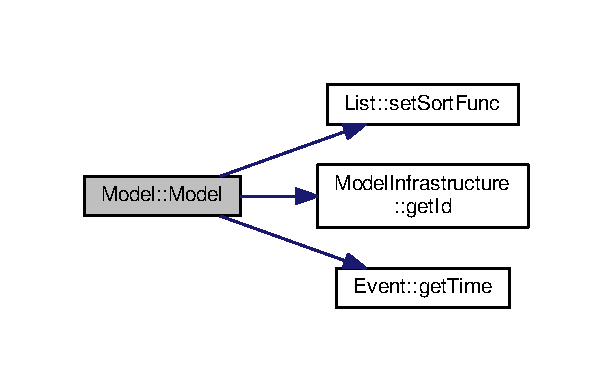
\includegraphics[width=294pt]{class_model_ae86e1403523e8036ba6366d1967ecac0_cgraph}
\end{center}
\end{figure}


\hypertarget{class_model_afdedf278781f785abeecf5f450e43653}{\index{Model@{Model}!Model@{Model}}
\index{Model@{Model}!Model@{Model}}
\subsubsection[{Model}]{\setlength{\rightskip}{0pt plus 5cm}Model\-::\-Model (
\begin{DoxyParamCaption}
\item[{const {\bf Model} \&}]{orig}
\end{DoxyParamCaption}
)}}\label{class_model_afdedf278781f785abeecf5f450e43653}
\hypertarget{class_model_ad6ebd2062a0b823db841a0b88baac4c0}{\index{Model@{Model}!$\sim$\-Model@{$\sim$\-Model}}
\index{$\sim$\-Model@{$\sim$\-Model}!Model@{Model}}
\subsubsection[{$\sim$\-Model}]{\setlength{\rightskip}{0pt plus 5cm}Model\-::$\sim$\-Model (
\begin{DoxyParamCaption}
{}
\end{DoxyParamCaption}
)\hspace{0.3cm}{\ttfamily [virtual]}}}\label{class_model_ad6ebd2062a0b823db841a0b88baac4c0}


\subsection{Member Function Documentation}
\hypertarget{class_model_a0b632c73e85b352d7ea914b30bb455f9}{\index{Model@{Model}!add\-Trace\-Error\-Listener@{add\-Trace\-Error\-Listener}}
\index{add\-Trace\-Error\-Listener@{add\-Trace\-Error\-Listener}!Model@{Model}}
\subsubsection[{add\-Trace\-Error\-Listener}]{\setlength{\rightskip}{0pt plus 5cm}void Model\-::add\-Trace\-Error\-Listener (
\begin{DoxyParamCaption}
\item[{{\bf trace\-Error\-Listener}}]{trace\-Error\-Listener}
\end{DoxyParamCaption}
)}}\label{class_model_a0b632c73e85b352d7ea914b30bb455f9}
\hypertarget{class_model_a144f16211e64bdc0ac4622cda5f5f4ae}{\index{Model@{Model}!add\-Trace\-Listener@{add\-Trace\-Listener}}
\index{add\-Trace\-Listener@{add\-Trace\-Listener}!Model@{Model}}
\subsubsection[{add\-Trace\-Listener}]{\setlength{\rightskip}{0pt plus 5cm}void Model\-::add\-Trace\-Listener (
\begin{DoxyParamCaption}
\item[{{\bf trace\-Listener}}]{trace\-Listener}
\end{DoxyParamCaption}
)}}\label{class_model_a144f16211e64bdc0ac4622cda5f5f4ae}
\hypertarget{class_model_ad94736b0e6c53b3dedd112f21506092a}{\index{Model@{Model}!add\-Trace\-Report\-Listener@{add\-Trace\-Report\-Listener}}
\index{add\-Trace\-Report\-Listener@{add\-Trace\-Report\-Listener}!Model@{Model}}
\subsubsection[{add\-Trace\-Report\-Listener}]{\setlength{\rightskip}{0pt plus 5cm}void Model\-::add\-Trace\-Report\-Listener (
\begin{DoxyParamCaption}
\item[{{\bf trace\-Listener}}]{trace\-Report\-Listener}
\end{DoxyParamCaption}
)}}\label{class_model_ad94736b0e6c53b3dedd112f21506092a}
\hypertarget{class_model_a06f7035263e7ad33360651a9569ed2d6}{\index{Model@{Model}!add\-Trace\-Simulation\-Listener@{add\-Trace\-Simulation\-Listener}}
\index{add\-Trace\-Simulation\-Listener@{add\-Trace\-Simulation\-Listener}!Model@{Model}}
\subsubsection[{add\-Trace\-Simulation\-Listener}]{\setlength{\rightskip}{0pt plus 5cm}void Model\-::add\-Trace\-Simulation\-Listener (
\begin{DoxyParamCaption}
\item[{{\bf trace\-Simulation\-Listener}}]{trace\-Simulation\-Listener}
\end{DoxyParamCaption}
)}}\label{class_model_a06f7035263e7ad33360651a9569ed2d6}
\hypertarget{class_model_ae3b293adffbef6fd254d661ceeb2e116}{\index{Model@{Model}!check\-Model@{check\-Model}}
\index{check\-Model@{check\-Model}!Model@{Model}}
\subsubsection[{check\-Model}]{\setlength{\rightskip}{0pt plus 5cm}bool Model\-::check\-Model (
\begin{DoxyParamCaption}
{}
\end{DoxyParamCaption}
)}}\label{class_model_ae3b293adffbef6fd254d661ceeb2e116}


Here is the call graph for this function\-:\nopagebreak
\begin{figure}[H]
\begin{center}
\leavevmode
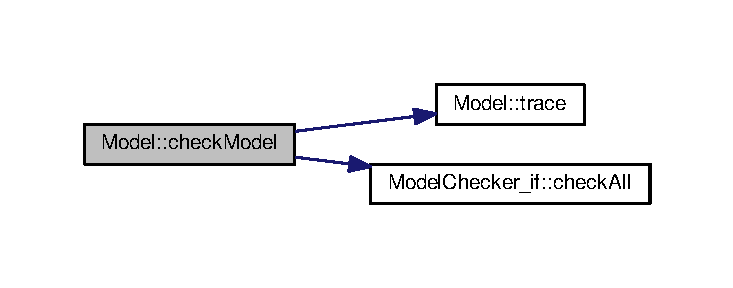
\includegraphics[width=350pt]{class_model_ae3b293adffbef6fd254d661ceeb2e116_cgraph}
\end{center}
\end{figure}


\hypertarget{class_model_a9b539226cc78c36bfe911252e9ccd055}{\index{Model@{Model}!get\-Analyst\-Name@{get\-Analyst\-Name}}
\index{get\-Analyst\-Name@{get\-Analyst\-Name}!Model@{Model}}
\subsubsection[{get\-Analyst\-Name}]{\setlength{\rightskip}{0pt plus 5cm}std\-::string Model\-::get\-Analyst\-Name (
\begin{DoxyParamCaption}
{}
\end{DoxyParamCaption}
) const}}\label{class_model_a9b539226cc78c36bfe911252e9ccd055}
\hypertarget{class_model_ae5773d78fc47cb35be7fbeb74b7d63e4}{\index{Model@{Model}!get\-Components@{get\-Components}}
\index{get\-Components@{get\-Components}!Model@{Model}}
\subsubsection[{get\-Components}]{\setlength{\rightskip}{0pt plus 5cm}{\bf List}$<$ {\bf Model\-Component} $\ast$ $>$ $\ast$ Model\-::get\-Components (
\begin{DoxyParamCaption}
{}
\end{DoxyParamCaption}
) const}}\label{class_model_ae5773d78fc47cb35be7fbeb74b7d63e4}
\hypertarget{class_model_a40ad9af9a5cebe907d483fb51d0f4974}{\index{Model@{Model}!get\-Description@{get\-Description}}
\index{get\-Description@{get\-Description}!Model@{Model}}
\subsubsection[{get\-Description}]{\setlength{\rightskip}{0pt plus 5cm}std\-::string Model\-::get\-Description (
\begin{DoxyParamCaption}
{}
\end{DoxyParamCaption}
) const}}\label{class_model_a40ad9af9a5cebe907d483fb51d0f4974}
\hypertarget{class_model_ae09e777b481981772818ea3fd2880c4c}{\index{Model@{Model}!get\-Entities@{get\-Entities}}
\index{get\-Entities@{get\-Entities}!Model@{Model}}
\subsubsection[{get\-Entities}]{\setlength{\rightskip}{0pt plus 5cm}{\bf List}$<$ {\bf Entity} $\ast$ $>$ $\ast$ Model\-::get\-Entities (
\begin{DoxyParamCaption}
{}
\end{DoxyParamCaption}
) const}}\label{class_model_ae09e777b481981772818ea3fd2880c4c}
The future events list chronologically sorted; Events are scheduled by components when processing other events, and a replication evolves over time by sequentially processing the very first event in this list. It's initialized with events first described by source components (Source\-Component\-Model) 

Here is the call graph for this function\-:\nopagebreak
\begin{figure}[H]
\begin{center}
\leavevmode
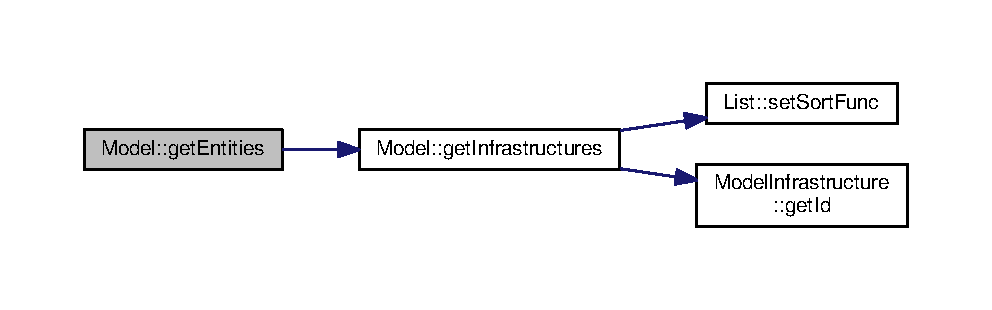
\includegraphics[width=350pt]{class_model_ae09e777b481981772818ea3fd2880c4c_cgraph}
\end{center}
\end{figure}


\hypertarget{class_model_ae0d77f48384e180cfabb8fd8ed16e4db}{\index{Model@{Model}!get\-Error\-Messages@{get\-Error\-Messages}}
\index{get\-Error\-Messages@{get\-Error\-Messages}!Model@{Model}}
\subsubsection[{get\-Error\-Messages}]{\setlength{\rightskip}{0pt plus 5cm}{\bf List}$<$ std\-::string $>$ $\ast$ Model\-::get\-Error\-Messages (
\begin{DoxyParamCaption}
{}
\end{DoxyParamCaption}
) const}}\label{class_model_ae0d77f48384e180cfabb8fd8ed16e4db}
\hypertarget{class_model_a841c78bda0eb27c652c6921094dc5921}{\index{Model@{Model}!get\-Events@{get\-Events}}
\index{get\-Events@{get\-Events}!Model@{Model}}
\subsubsection[{get\-Events}]{\setlength{\rightskip}{0pt plus 5cm}{\bf List}$<$ {\bf Event} $\ast$ $>$ $\ast$ Model\-::get\-Events (
\begin{DoxyParamCaption}
{}
\end{DoxyParamCaption}
) const}}\label{class_model_a841c78bda0eb27c652c6921094dc5921}
A list of components that compose this model \hypertarget{class_model_abfd7753d30de6abea64b3f0846e097eb}{\index{Model@{Model}!get\-Id@{get\-Id}}
\index{get\-Id@{get\-Id}!Model@{Model}}
\subsubsection[{get\-Id}]{\setlength{\rightskip}{0pt plus 5cm}{\bf Util\-::identitifcation} Model\-::get\-Id (
\begin{DoxyParamCaption}
{}
\end{DoxyParamCaption}
) const}}\label{class_model_abfd7753d30de6abea64b3f0846e097eb}
\hypertarget{class_model_ab460d8d215b5e4fb353f129c04493fa5}{\index{Model@{Model}!get\-Infrastructure@{get\-Infrastructure}}
\index{get\-Infrastructure@{get\-Infrastructure}!Model@{Model}}
\subsubsection[{get\-Infrastructure}]{\setlength{\rightskip}{0pt plus 5cm}{\bf Model\-Infrastructure} $\ast$ Model\-::get\-Infrastructure (
\begin{DoxyParamCaption}
\item[{std\-::string}]{infra\-Typename, }
\item[{{\bf Util\-::identitifcation}}]{id}
\end{DoxyParamCaption}
)}}\label{class_model_ab460d8d215b5e4fb353f129c04493fa5}


Here is the call graph for this function\-:\nopagebreak
\begin{figure}[H]
\begin{center}
\leavevmode
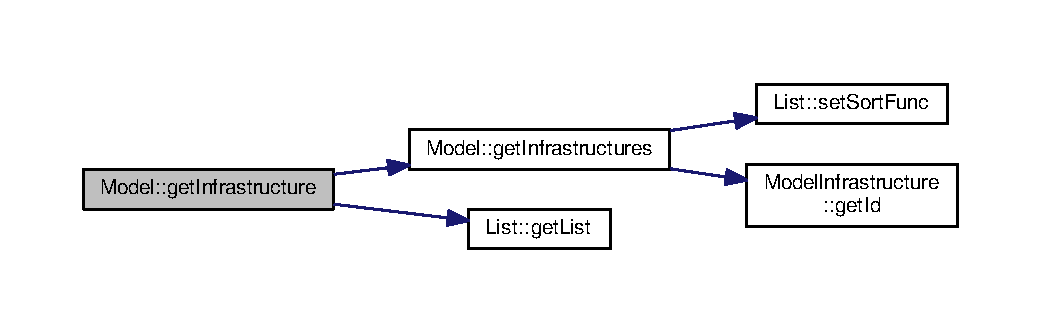
\includegraphics[width=350pt]{class_model_ab460d8d215b5e4fb353f129c04493fa5_cgraph}
\end{center}
\end{figure}


\hypertarget{class_model_ad6711b51ea9feeacb59eaf70cc8faaed}{\index{Model@{Model}!get\-Infrastructure@{get\-Infrastructure}}
\index{get\-Infrastructure@{get\-Infrastructure}!Model@{Model}}
\subsubsection[{get\-Infrastructure}]{\setlength{\rightskip}{0pt plus 5cm}{\bf Model\-Infrastructure} $\ast$ Model\-::get\-Infrastructure (
\begin{DoxyParamCaption}
\item[{std\-::string}]{infra\-Typename, }
\item[{std\-::string}]{name}
\end{DoxyParamCaption}
)}}\label{class_model_ad6711b51ea9feeacb59eaf70cc8faaed}


Here is the call graph for this function\-:\nopagebreak
\begin{figure}[H]
\begin{center}
\leavevmode
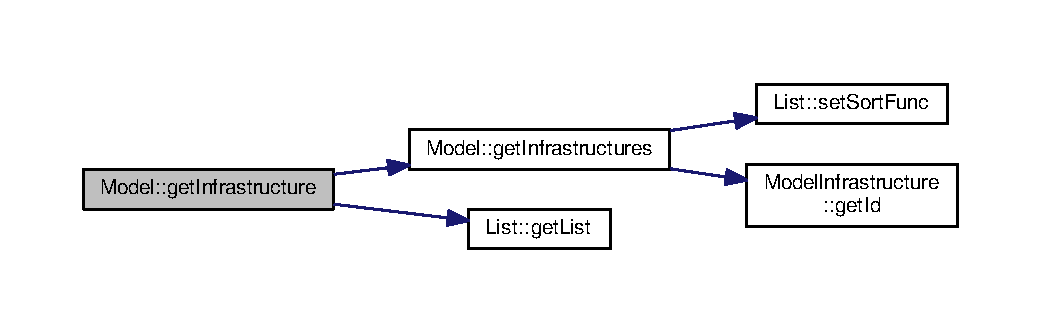
\includegraphics[width=350pt]{class_model_ad6711b51ea9feeacb59eaf70cc8faaed_cgraph}
\end{center}
\end{figure}


\hypertarget{class_model_a43ca6ff93bd0b9fbc4c2792962e6b4ed}{\index{Model@{Model}!get\-Infrastructures@{get\-Infrastructures}}
\index{get\-Infrastructures@{get\-Infrastructures}!Model@{Model}}
\subsubsection[{get\-Infrastructures}]{\setlength{\rightskip}{0pt plus 5cm}{\bf List}$<$ {\bf Model\-Infrastructure} $\ast$ $>$ $\ast$ Model\-::get\-Infrastructures (
\begin{DoxyParamCaption}
\item[{std\-::string}]{infra\-Typename}
\end{DoxyParamCaption}
) const}}\label{class_model_a43ca6ff93bd0b9fbc4c2792962e6b4ed}


Here is the call graph for this function\-:\nopagebreak
\begin{figure}[H]
\begin{center}
\leavevmode
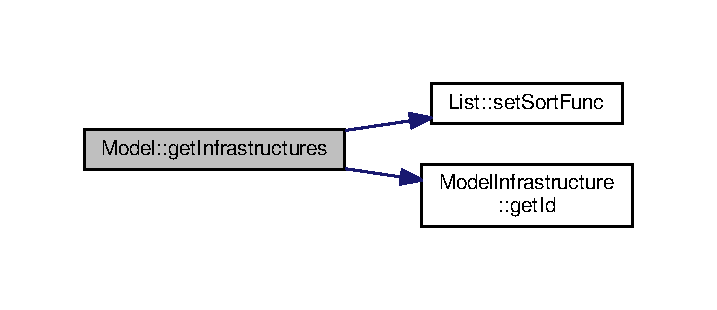
\includegraphics[width=344pt]{class_model_a43ca6ff93bd0b9fbc4c2792962e6b4ed_cgraph}
\end{center}
\end{figure}


\hypertarget{class_model_a1a1c7e795ee409d8e61c942db5f94d17}{\index{Model@{Model}!get\-Name@{get\-Name}}
\index{get\-Name@{get\-Name}!Model@{Model}}
\subsubsection[{get\-Name}]{\setlength{\rightskip}{0pt plus 5cm}std\-::string Model\-::get\-Name (
\begin{DoxyParamCaption}
{}
\end{DoxyParamCaption}
) const}}\label{class_model_a1a1c7e795ee409d8e61c942db5f94d17}
\hypertarget{class_model_af2fe357b860298f4977f8f48cee7115a}{\index{Model@{Model}!get\-Number\-Of\-Replications@{get\-Number\-Of\-Replications}}
\index{get\-Number\-Of\-Replications@{get\-Number\-Of\-Replications}!Model@{Model}}
\subsubsection[{get\-Number\-Of\-Replications}]{\setlength{\rightskip}{0pt plus 5cm}unsigned int Model\-::get\-Number\-Of\-Replications (
\begin{DoxyParamCaption}
{}
\end{DoxyParamCaption}
) const}}\label{class_model_af2fe357b860298f4977f8f48cee7115a}
\hypertarget{class_model_ae2197c7da38542ec199491c3d5797efd}{\index{Model@{Model}!get\-Project\-Title@{get\-Project\-Title}}
\index{get\-Project\-Title@{get\-Project\-Title}!Model@{Model}}
\subsubsection[{get\-Project\-Title}]{\setlength{\rightskip}{0pt plus 5cm}std\-::string Model\-::get\-Project\-Title (
\begin{DoxyParamCaption}
{}
\end{DoxyParamCaption}
) const}}\label{class_model_ae2197c7da38542ec199491c3d5797efd}
\hypertarget{class_model_a6bb4d4fbf90f49c990a00385a9df18d9}{\index{Model@{Model}!get\-Replication\-Length@{get\-Replication\-Length}}
\index{get\-Replication\-Length@{get\-Replication\-Length}!Model@{Model}}
\subsubsection[{get\-Replication\-Length}]{\setlength{\rightskip}{0pt plus 5cm}double Model\-::get\-Replication\-Length (
\begin{DoxyParamCaption}
{}
\end{DoxyParamCaption}
) const}}\label{class_model_a6bb4d4fbf90f49c990a00385a9df18d9}
\hypertarget{class_model_aeaba7aa3fb5a75f469b7617910eee446}{\index{Model@{Model}!get\-Replication\-Length\-Time\-Unit@{get\-Replication\-Length\-Time\-Unit}}
\index{get\-Replication\-Length\-Time\-Unit@{get\-Replication\-Length\-Time\-Unit}!Model@{Model}}
\subsubsection[{get\-Replication\-Length\-Time\-Unit}]{\setlength{\rightskip}{0pt plus 5cm}{\bf Util\-::\-Time\-Unit} Model\-::get\-Replication\-Length\-Time\-Unit (
\begin{DoxyParamCaption}
{}
\end{DoxyParamCaption}
) const}}\label{class_model_aeaba7aa3fb5a75f469b7617910eee446}
\hypertarget{class_model_a74eb096b8229aa036d11adeeb8787599}{\index{Model@{Model}!get\-Simulated\-Time@{get\-Simulated\-Time}}
\index{get\-Simulated\-Time@{get\-Simulated\-Time}!Model@{Model}}
\subsubsection[{get\-Simulated\-Time}]{\setlength{\rightskip}{0pt plus 5cm}double Model\-::get\-Simulated\-Time (
\begin{DoxyParamCaption}
{}
\end{DoxyParamCaption}
) const}}\label{class_model_a74eb096b8229aa036d11adeeb8787599}
\hypertarget{class_model_a3da1140b818632e728fd57445ab1880b}{\index{Model@{Model}!get\-Terminating\-Condition@{get\-Terminating\-Condition}}
\index{get\-Terminating\-Condition@{get\-Terminating\-Condition}!Model@{Model}}
\subsubsection[{get\-Terminating\-Condition}]{\setlength{\rightskip}{0pt plus 5cm}std\-::string Model\-::get\-Terminating\-Condition (
\begin{DoxyParamCaption}
{}
\end{DoxyParamCaption}
) const}}\label{class_model_a3da1140b818632e728fd57445ab1880b}
\hypertarget{class_model_a0fa341be1579f13861af2eda84d4f840}{\index{Model@{Model}!get\-Trace\-Level@{get\-Trace\-Level}}
\index{get\-Trace\-Level@{get\-Trace\-Level}!Model@{Model}}
\subsubsection[{get\-Trace\-Level}]{\setlength{\rightskip}{0pt plus 5cm}{\bf Util\-::\-Trace\-Level} Model\-::get\-Trace\-Level (
\begin{DoxyParamCaption}
{}
\end{DoxyParamCaption}
) const}}\label{class_model_a0fa341be1579f13861af2eda84d4f840}
\hypertarget{class_model_a073ecbf56dfd06e46af31bbd67a0402d}{\index{Model@{Model}!get\-Version@{get\-Version}}
\index{get\-Version@{get\-Version}!Model@{Model}}
\subsubsection[{get\-Version}]{\setlength{\rightskip}{0pt plus 5cm}std\-::string Model\-::get\-Version (
\begin{DoxyParamCaption}
{}
\end{DoxyParamCaption}
) const}}\label{class_model_a073ecbf56dfd06e46af31bbd67a0402d}
\hypertarget{class_model_aa7b278f97a29269a18dbcbb6513f39da}{\index{Model@{Model}!get\-Warm\-Up\-Period@{get\-Warm\-Up\-Period}}
\index{get\-Warm\-Up\-Period@{get\-Warm\-Up\-Period}!Model@{Model}}
\subsubsection[{get\-Warm\-Up\-Period}]{\setlength{\rightskip}{0pt plus 5cm}double Model\-::get\-Warm\-Up\-Period (
\begin{DoxyParamCaption}
{}
\end{DoxyParamCaption}
) const}}\label{class_model_aa7b278f97a29269a18dbcbb6513f39da}
\hypertarget{class_model_a12a97aefe53ac31b8e7801b50a87715a}{\index{Model@{Model}!get\-Warm\-Up\-Period\-Time\-Unit@{get\-Warm\-Up\-Period\-Time\-Unit}}
\index{get\-Warm\-Up\-Period\-Time\-Unit@{get\-Warm\-Up\-Period\-Time\-Unit}!Model@{Model}}
\subsubsection[{get\-Warm\-Up\-Period\-Time\-Unit}]{\setlength{\rightskip}{0pt plus 5cm}{\bf Util\-::\-Time\-Unit} Model\-::get\-Warm\-Up\-Period\-Time\-Unit (
\begin{DoxyParamCaption}
{}
\end{DoxyParamCaption}
) const}}\label{class_model_a12a97aefe53ac31b8e7801b50a87715a}
\hypertarget{class_model_aefe1365d9a032fe1ac62991f45446d6a}{\index{Model@{Model}!is\-Initialize\-Statistics@{is\-Initialize\-Statistics}}
\index{is\-Initialize\-Statistics@{is\-Initialize\-Statistics}!Model@{Model}}
\subsubsection[{is\-Initialize\-Statistics}]{\setlength{\rightskip}{0pt plus 5cm}bool Model\-::is\-Initialize\-Statistics (
\begin{DoxyParamCaption}
{}
\end{DoxyParamCaption}
) const}}\label{class_model_aefe1365d9a032fe1ac62991f45446d6a}
\hypertarget{class_model_afd5e0285a55278e266045112ef795868}{\index{Model@{Model}!is\-Initialize\-System@{is\-Initialize\-System}}
\index{is\-Initialize\-System@{is\-Initialize\-System}!Model@{Model}}
\subsubsection[{is\-Initialize\-System}]{\setlength{\rightskip}{0pt plus 5cm}bool Model\-::is\-Initialize\-System (
\begin{DoxyParamCaption}
{}
\end{DoxyParamCaption}
) const}}\label{class_model_afd5e0285a55278e266045112ef795868}
\hypertarget{class_model_a1dda07db7bddff456907067eeeb5c21a}{\index{Model@{Model}!is\-Pause\-On\-Event@{is\-Pause\-On\-Event}}
\index{is\-Pause\-On\-Event@{is\-Pause\-On\-Event}!Model@{Model}}
\subsubsection[{is\-Pause\-On\-Event}]{\setlength{\rightskip}{0pt plus 5cm}bool Model\-::is\-Pause\-On\-Event (
\begin{DoxyParamCaption}
{}
\end{DoxyParamCaption}
) const}}\label{class_model_a1dda07db7bddff456907067eeeb5c21a}
\hypertarget{class_model_a269e5b3c45f3c7ce606205fec8f0b3b4}{\index{Model@{Model}!is\-Pause\-On\-Replication@{is\-Pause\-On\-Replication}}
\index{is\-Pause\-On\-Replication@{is\-Pause\-On\-Replication}!Model@{Model}}
\subsubsection[{is\-Pause\-On\-Replication}]{\setlength{\rightskip}{0pt plus 5cm}bool Model\-::is\-Pause\-On\-Replication (
\begin{DoxyParamCaption}
{}
\end{DoxyParamCaption}
) const}}\label{class_model_a269e5b3c45f3c7ce606205fec8f0b3b4}
\hypertarget{class_model_a597bdaa89e9b6b396bded780e6d32fdf}{\index{Model@{Model}!is\-Running@{is\-Running}}
\index{is\-Running@{is\-Running}!Model@{Model}}
\subsubsection[{is\-Running}]{\setlength{\rightskip}{0pt plus 5cm}bool Model\-::is\-Running (
\begin{DoxyParamCaption}
{}
\end{DoxyParamCaption}
) const}}\label{class_model_a597bdaa89e9b6b396bded780e6d32fdf}
The current time in the model being simulated, i.\-e., the instant when the current event was triggered \hypertarget{class_model_a8d47ce2750e22e14e5249b724cdf4fd3}{\index{Model@{Model}!is\-Saved@{is\-Saved}}
\index{is\-Saved@{is\-Saved}!Model@{Model}}
\subsubsection[{is\-Saved}]{\setlength{\rightskip}{0pt plus 5cm}bool Model\-::is\-Saved (
\begin{DoxyParamCaption}
{}
\end{DoxyParamCaption}
) const}}\label{class_model_a8d47ce2750e22e14e5249b724cdf4fd3}
\hypertarget{class_model_a8bc24806234d057bedb4262ecc090bf0}{\index{Model@{Model}!is\-Step\-By\-Step@{is\-Step\-By\-Step}}
\index{is\-Step\-By\-Step@{is\-Step\-By\-Step}!Model@{Model}}
\subsubsection[{is\-Step\-By\-Step}]{\setlength{\rightskip}{0pt plus 5cm}bool Model\-::is\-Step\-By\-Step (
\begin{DoxyParamCaption}
{}
\end{DoxyParamCaption}
) const}}\label{class_model_a8bc24806234d057bedb4262ecc090bf0}
\hypertarget{class_model_aba57e8b62d4dcc3ac8e3037933fa6f04}{\index{Model@{Model}!load\-Model@{load\-Model}}
\index{load\-Model@{load\-Model}!Model@{Model}}
\subsubsection[{load\-Model}]{\setlength{\rightskip}{0pt plus 5cm}bool Model\-::load\-Model (
\begin{DoxyParamCaption}
\item[{std\-::string}]{filename}
\end{DoxyParamCaption}
)}}\label{class_model_aba57e8b62d4dcc3ac8e3037933fa6f04}


Here is the call graph for this function\-:\nopagebreak
\begin{figure}[H]
\begin{center}
\leavevmode
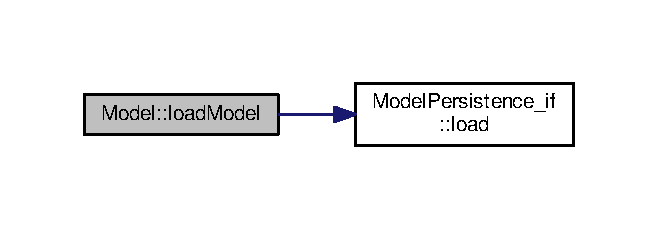
\includegraphics[width=316pt]{class_model_aba57e8b62d4dcc3ac8e3037933fa6f04_cgraph}
\end{center}
\end{figure}


\hypertarget{class_model_a5ea283e339b50c0b77040bf908e25af3}{\index{Model@{Model}!parse\-Expression@{parse\-Expression}}
\index{parse\-Expression@{parse\-Expression}!Model@{Model}}
\subsubsection[{parse\-Expression}]{\setlength{\rightskip}{0pt plus 5cm}double Model\-::parse\-Expression (
\begin{DoxyParamCaption}
\item[{const std\-::string}]{expression}
\end{DoxyParamCaption}
)}}\label{class_model_a5ea283e339b50c0b77040bf908e25af3}
Used by components (\hyperlink{class_model_component}{Model\-Component}) to send entities to another specific component, usually the next one connected to it, or used by the model itself, when processing an event (\hyperlink{class_event}{Event}). 

Here is the call graph for this function\-:\nopagebreak
\begin{figure}[H]
\begin{center}
\leavevmode
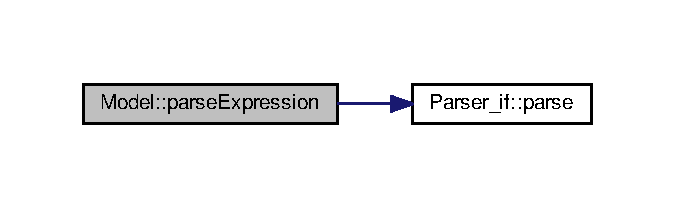
\includegraphics[width=324pt]{class_model_a5ea283e339b50c0b77040bf908e25af3_cgraph}
\end{center}
\end{figure}


\hypertarget{class_model_ab10d4bdc433d11bf4bb7117675091d8c}{\index{Model@{Model}!pause\-Simulation@{pause\-Simulation}}
\index{pause\-Simulation@{pause\-Simulation}!Model@{Model}}
\subsubsection[{pause\-Simulation}]{\setlength{\rightskip}{0pt plus 5cm}void Model\-::pause\-Simulation (
\begin{DoxyParamCaption}
{}
\end{DoxyParamCaption}
)}}\label{class_model_ab10d4bdc433d11bf4bb7117675091d8c}
Starts a sequential execution of a simulation, ie, a set of repliations of this model \hypertarget{class_model_ae62bb3a21cd56fbf9d34195edf2fb9e0}{\index{Model@{Model}!remove\-Entity@{remove\-Entity}}
\index{remove\-Entity@{remove\-Entity}!Model@{Model}}
\subsubsection[{remove\-Entity}]{\setlength{\rightskip}{0pt plus 5cm}void Model\-::remove\-Entity (
\begin{DoxyParamCaption}
\item[{{\bf Entity} $\ast$}]{entity, }
\item[{bool}]{collect\-Statistics}
\end{DoxyParamCaption}
)}}\label{class_model_ae62bb3a21cd56fbf9d34195edf2fb9e0}
Verifies if a symbol defined in a component (\hyperlink{class_model_component}{Model\-Component}) or infrastructure is syntactically valid and addresses existing components or infrastructures. It's used only by and directed by the component that defines the symbol. 

Here is the call graph for this function\-:\nopagebreak
\begin{figure}[H]
\begin{center}
\leavevmode
\includegraphics[width=350pt]{class_model_ae62bb3a21cd56fbf9d34195edf2fb9e0_cgraph}
\end{center}
\end{figure}


\hypertarget{class_model_a8be70da19c6c315269acc5a3fd2e3b7d}{\index{Model@{Model}!restart\-Simulation@{restart\-Simulation}}
\index{restart\-Simulation@{restart\-Simulation}!Model@{Model}}
\subsubsection[{restart\-Simulation}]{\setlength{\rightskip}{0pt plus 5cm}void Model\-::restart\-Simulation (
\begin{DoxyParamCaption}
{}
\end{DoxyParamCaption}
)}}\label{class_model_a8be70da19c6c315269acc5a3fd2e3b7d}
\hypertarget{class_model_ae099910781f5267a51fb5d607246af4a}{\index{Model@{Model}!save\-Model@{save\-Model}}
\index{save\-Model@{save\-Model}!Model@{Model}}
\subsubsection[{save\-Model}]{\setlength{\rightskip}{0pt plus 5cm}bool Model\-::save\-Model (
\begin{DoxyParamCaption}
\item[{std\-::string}]{filename}
\end{DoxyParamCaption}
)}}\label{class_model_ae099910781f5267a51fb5d607246af4a}


Here is the call graph for this function\-:\nopagebreak
\begin{figure}[H]
\begin{center}
\leavevmode
\includegraphics[width=318pt]{class_model_ae099910781f5267a51fb5d607246af4a_cgraph}
\end{center}
\end{figure}


\hypertarget{class_model_a244dff6d6bef962b0d95fbe712954079}{\index{Model@{Model}!send\-Entity\-To\-Component@{send\-Entity\-To\-Component}}
\index{send\-Entity\-To\-Component@{send\-Entity\-To\-Component}!Model@{Model}}
\subsubsection[{send\-Entity\-To\-Component}]{\setlength{\rightskip}{0pt plus 5cm}void Model\-::send\-Entity\-To\-Component (
\begin{DoxyParamCaption}
\item[{{\bf Entity} $\ast$}]{entity, }
\item[{{\bf Model\-Component} $\ast$}]{component, }
\item[{double}]{time\-Delay}
\end{DoxyParamCaption}
)}}\label{class_model_a244dff6d6bef962b0d95fbe712954079}


Here is the call graph for this function\-:\nopagebreak
\begin{figure}[H]
\begin{center}
\leavevmode
\includegraphics[width=350pt]{class_model_a244dff6d6bef962b0d95fbe712954079_cgraph}
\end{center}
\end{figure}


\hypertarget{class_model_a52c044c61c8411b083006d2c5fbe0abf}{\index{Model@{Model}!set\-Analyst\-Name@{set\-Analyst\-Name}}
\index{set\-Analyst\-Name@{set\-Analyst\-Name}!Model@{Model}}
\subsubsection[{set\-Analyst\-Name}]{\setlength{\rightskip}{0pt plus 5cm}void Model\-::set\-Analyst\-Name (
\begin{DoxyParamCaption}
\item[{std\-::string}]{\-\_\-analyst\-Name}
\end{DoxyParamCaption}
)}}\label{class_model_a52c044c61c8411b083006d2c5fbe0abf}
\hypertarget{class_model_a84eb0333d18ac7f8a684d1cd32c64dbd}{\index{Model@{Model}!set\-Description@{set\-Description}}
\index{set\-Description@{set\-Description}!Model@{Model}}
\subsubsection[{set\-Description}]{\setlength{\rightskip}{0pt plus 5cm}void Model\-::set\-Description (
\begin{DoxyParamCaption}
\item[{std\-::string}]{\-\_\-description}
\end{DoxyParamCaption}
)}}\label{class_model_a84eb0333d18ac7f8a684d1cd32c64dbd}
\hypertarget{class_model_a2fe72bb622b3d75479822f68710a36c7}{\index{Model@{Model}!set\-Initialize\-Statistics@{set\-Initialize\-Statistics}}
\index{set\-Initialize\-Statistics@{set\-Initialize\-Statistics}!Model@{Model}}
\subsubsection[{set\-Initialize\-Statistics}]{\setlength{\rightskip}{0pt plus 5cm}void Model\-::set\-Initialize\-Statistics (
\begin{DoxyParamCaption}
\item[{bool}]{\-\_\-initialize\-Statistics}
\end{DoxyParamCaption}
)}}\label{class_model_a2fe72bb622b3d75479822f68710a36c7}
\hypertarget{class_model_ac1299b28921f4d246319b2624e4ad98f}{\index{Model@{Model}!set\-Initialize\-System@{set\-Initialize\-System}}
\index{set\-Initialize\-System@{set\-Initialize\-System}!Model@{Model}}
\subsubsection[{set\-Initialize\-System}]{\setlength{\rightskip}{0pt plus 5cm}void Model\-::set\-Initialize\-System (
\begin{DoxyParamCaption}
\item[{bool}]{\-\_\-initialize\-System}
\end{DoxyParamCaption}
)}}\label{class_model_ac1299b28921f4d246319b2624e4ad98f}
\hypertarget{class_model_a2aab01a2871b2924eeb3c265267fabef}{\index{Model@{Model}!set\-Name@{set\-Name}}
\index{set\-Name@{set\-Name}!Model@{Model}}
\subsubsection[{set\-Name}]{\setlength{\rightskip}{0pt plus 5cm}void Model\-::set\-Name (
\begin{DoxyParamCaption}
\item[{std\-::string}]{\-\_\-name}
\end{DoxyParamCaption}
)}}\label{class_model_a2aab01a2871b2924eeb3c265267fabef}
\hypertarget{class_model_a55d597e867b5c3e27cb2e1511414e7f3}{\index{Model@{Model}!set\-Number\-Of\-Replications@{set\-Number\-Of\-Replications}}
\index{set\-Number\-Of\-Replications@{set\-Number\-Of\-Replications}!Model@{Model}}
\subsubsection[{set\-Number\-Of\-Replications}]{\setlength{\rightskip}{0pt plus 5cm}void Model\-::set\-Number\-Of\-Replications (
\begin{DoxyParamCaption}
\item[{unsigned int}]{\-\_\-number\-Of\-Replications}
\end{DoxyParamCaption}
)}}\label{class_model_a55d597e867b5c3e27cb2e1511414e7f3}
\hypertarget{class_model_a99238439363a292fe1fc503eb2157a55}{\index{Model@{Model}!set\-Pause\-On\-Event@{set\-Pause\-On\-Event}}
\index{set\-Pause\-On\-Event@{set\-Pause\-On\-Event}!Model@{Model}}
\subsubsection[{set\-Pause\-On\-Event}]{\setlength{\rightskip}{0pt plus 5cm}void Model\-::set\-Pause\-On\-Event (
\begin{DoxyParamCaption}
\item[{bool}]{\-\_\-pause\-On\-Event}
\end{DoxyParamCaption}
)}}\label{class_model_a99238439363a292fe1fc503eb2157a55}
\hypertarget{class_model_ae1f205bd8b328b3785694567eaeb77ef}{\index{Model@{Model}!set\-Pause\-On\-Replication@{set\-Pause\-On\-Replication}}
\index{set\-Pause\-On\-Replication@{set\-Pause\-On\-Replication}!Model@{Model}}
\subsubsection[{set\-Pause\-On\-Replication}]{\setlength{\rightskip}{0pt plus 5cm}void Model\-::set\-Pause\-On\-Replication (
\begin{DoxyParamCaption}
\item[{bool}]{\-\_\-pause\-Between\-Replications}
\end{DoxyParamCaption}
)}}\label{class_model_ae1f205bd8b328b3785694567eaeb77ef}
\hypertarget{class_model_a97ce94d618caee4364e82a8790f00052}{\index{Model@{Model}!set\-Project\-Title@{set\-Project\-Title}}
\index{set\-Project\-Title@{set\-Project\-Title}!Model@{Model}}
\subsubsection[{set\-Project\-Title}]{\setlength{\rightskip}{0pt plus 5cm}void Model\-::set\-Project\-Title (
\begin{DoxyParamCaption}
\item[{std\-::string}]{\-\_\-project\-Title}
\end{DoxyParamCaption}
)}}\label{class_model_a97ce94d618caee4364e82a8790f00052}
\hypertarget{class_model_a5be13e4bb83891e8caed52b3eae1470f}{\index{Model@{Model}!set\-Replication\-Length@{set\-Replication\-Length}}
\index{set\-Replication\-Length@{set\-Replication\-Length}!Model@{Model}}
\subsubsection[{set\-Replication\-Length}]{\setlength{\rightskip}{0pt plus 5cm}void Model\-::set\-Replication\-Length (
\begin{DoxyParamCaption}
\item[{double}]{\-\_\-replication\-Length}
\end{DoxyParamCaption}
)}}\label{class_model_a5be13e4bb83891e8caed52b3eae1470f}
\hypertarget{class_model_a0261d2009ad7a3f9025e31cf02e6297a}{\index{Model@{Model}!set\-Replication\-Length\-Time\-Unit@{set\-Replication\-Length\-Time\-Unit}}
\index{set\-Replication\-Length\-Time\-Unit@{set\-Replication\-Length\-Time\-Unit}!Model@{Model}}
\subsubsection[{set\-Replication\-Length\-Time\-Unit}]{\setlength{\rightskip}{0pt plus 5cm}void Model\-::set\-Replication\-Length\-Time\-Unit (
\begin{DoxyParamCaption}
\item[{{\bf Util\-::\-Time\-Unit}}]{\-\_\-replication\-Length\-Time\-Unit}
\end{DoxyParamCaption}
)}}\label{class_model_a0261d2009ad7a3f9025e31cf02e6297a}
\hypertarget{class_model_a2b4b1bb4e9c082e8b0c893a35f5a8f53}{\index{Model@{Model}!set\-Step\-By\-Step@{set\-Step\-By\-Step}}
\index{set\-Step\-By\-Step@{set\-Step\-By\-Step}!Model@{Model}}
\subsubsection[{set\-Step\-By\-Step}]{\setlength{\rightskip}{0pt plus 5cm}void Model\-::set\-Step\-By\-Step (
\begin{DoxyParamCaption}
\item[{bool}]{\-\_\-step\-By\-Step}
\end{DoxyParamCaption}
)}}\label{class_model_a2b4b1bb4e9c082e8b0c893a35f5a8f53}
\hypertarget{class_model_a480b4220ecfe82a1826ca29366a8d2b6}{\index{Model@{Model}!set\-Terminating\-Condition@{set\-Terminating\-Condition}}
\index{set\-Terminating\-Condition@{set\-Terminating\-Condition}!Model@{Model}}
\subsubsection[{set\-Terminating\-Condition}]{\setlength{\rightskip}{0pt plus 5cm}void Model\-::set\-Terminating\-Condition (
\begin{DoxyParamCaption}
\item[{std\-::string}]{\-\_\-terminating\-Condition}
\end{DoxyParamCaption}
)}}\label{class_model_a480b4220ecfe82a1826ca29366a8d2b6}
\hypertarget{class_model_a538fdc09de27b077b4e4c84fdc78a61e}{\index{Model@{Model}!set\-Trace\-Level@{set\-Trace\-Level}}
\index{set\-Trace\-Level@{set\-Trace\-Level}!Model@{Model}}
\subsubsection[{set\-Trace\-Level}]{\setlength{\rightskip}{0pt plus 5cm}void Model\-::set\-Trace\-Level (
\begin{DoxyParamCaption}
\item[{{\bf Util\-::\-Trace\-Level}}]{\-\_\-trace\-Level}
\end{DoxyParamCaption}
)}}\label{class_model_a538fdc09de27b077b4e4c84fdc78a61e}
\hypertarget{class_model_a630f152feb166751ecf53e5c628a7826}{\index{Model@{Model}!set\-Version@{set\-Version}}
\index{set\-Version@{set\-Version}!Model@{Model}}
\subsubsection[{set\-Version}]{\setlength{\rightskip}{0pt plus 5cm}void Model\-::set\-Version (
\begin{DoxyParamCaption}
\item[{std\-::string}]{\-\_\-version}
\end{DoxyParamCaption}
)}}\label{class_model_a630f152feb166751ecf53e5c628a7826}
\hypertarget{class_model_ac6e4c4bd49b999b2f6ce5ad97d45bbae}{\index{Model@{Model}!set\-Warm\-Up\-Period@{set\-Warm\-Up\-Period}}
\index{set\-Warm\-Up\-Period@{set\-Warm\-Up\-Period}!Model@{Model}}
\subsubsection[{set\-Warm\-Up\-Period}]{\setlength{\rightskip}{0pt plus 5cm}void Model\-::set\-Warm\-Up\-Period (
\begin{DoxyParamCaption}
\item[{double}]{\-\_\-warm\-Up\-Period}
\end{DoxyParamCaption}
)}}\label{class_model_ac6e4c4bd49b999b2f6ce5ad97d45bbae}
\hypertarget{class_model_a864c1a3f96cd05b83894042e41ef5ea6}{\index{Model@{Model}!set\-Warm\-Up\-Period\-Time\-Unit@{set\-Warm\-Up\-Period\-Time\-Unit}}
\index{set\-Warm\-Up\-Period\-Time\-Unit@{set\-Warm\-Up\-Period\-Time\-Unit}!Model@{Model}}
\subsubsection[{set\-Warm\-Up\-Period\-Time\-Unit}]{\setlength{\rightskip}{0pt plus 5cm}void Model\-::set\-Warm\-Up\-Period\-Time\-Unit (
\begin{DoxyParamCaption}
\item[{{\bf Util\-::\-Time\-Unit}}]{\-\_\-warm\-Up\-Period\-Time\-Unit}
\end{DoxyParamCaption}
)}}\label{class_model_a864c1a3f96cd05b83894042e41ef5ea6}
\hypertarget{class_model_a44c66f552308e7a6a5701801186a8637}{\index{Model@{Model}!show\-Reports@{show\-Reports}}
\index{show\-Reports@{show\-Reports}!Model@{Model}}
\subsubsection[{show\-Reports}]{\setlength{\rightskip}{0pt plus 5cm}void Model\-::show\-Reports (
\begin{DoxyParamCaption}
{}
\end{DoxyParamCaption}
)}}\label{class_model_a44c66f552308e7a6a5701801186a8637}
\hypertarget{class_model_a6fd6613a5141552a6493eb3a840cde24}{\index{Model@{Model}!start\-Simulation@{start\-Simulation}}
\index{start\-Simulation@{start\-Simulation}!Model@{Model}}
\subsubsection[{start\-Simulation}]{\setlength{\rightskip}{0pt plus 5cm}void Model\-::start\-Simulation (
\begin{DoxyParamCaption}
{}
\end{DoxyParamCaption}
)}}\label{class_model_a6fd6613a5141552a6493eb3a840cde24}


Here is the call graph for this function\-:\nopagebreak
\begin{figure}[H]
\begin{center}
\leavevmode
\includegraphics[width=350pt]{class_model_a6fd6613a5141552a6493eb3a840cde24_cgraph}
\end{center}
\end{figure}


\hypertarget{class_model_a025b6ab3112a1df6f7773389b096302c}{\index{Model@{Model}!step\-Simulation@{step\-Simulation}}
\index{step\-Simulation@{step\-Simulation}!Model@{Model}}
\subsubsection[{step\-Simulation}]{\setlength{\rightskip}{0pt plus 5cm}void Model\-::step\-Simulation (
\begin{DoxyParamCaption}
{}
\end{DoxyParamCaption}
)}}\label{class_model_a025b6ab3112a1df6f7773389b096302c}


Here is the call graph for this function\-:\nopagebreak
\begin{figure}[H]
\begin{center}
\leavevmode
\includegraphics[width=322pt]{class_model_a025b6ab3112a1df6f7773389b096302c_cgraph}
\end{center}
\end{figure}


\hypertarget{class_model_a6452e846a5e560220236b7a59f1dd84b}{\index{Model@{Model}!stop\-Simulation@{stop\-Simulation}}
\index{stop\-Simulation@{stop\-Simulation}!Model@{Model}}
\subsubsection[{stop\-Simulation}]{\setlength{\rightskip}{0pt plus 5cm}void Model\-::stop\-Simulation (
\begin{DoxyParamCaption}
{}
\end{DoxyParamCaption}
)}}\label{class_model_a6452e846a5e560220236b7a59f1dd84b}
Executes the processing of a single event, the next one in the future events list \hypertarget{class_model_a5de086b514742e84b61ac9a7b128ae8b}{\index{Model@{Model}!trace@{trace}}
\index{trace@{trace}!Model@{Model}}
\subsubsection[{trace}]{\setlength{\rightskip}{0pt plus 5cm}void Model\-::trace (
\begin{DoxyParamCaption}
\item[{{\bf Util\-::\-Trace\-Level}}]{tracelevel, }
\item[{std\-::string}]{text}
\end{DoxyParamCaption}
)}}\label{class_model_a5de086b514742e84b61ac9a7b128ae8b}
\hypertarget{class_model_a092b7062edcb59344f286d858ed10fac}{\index{Model@{Model}!trace\-Error@{trace\-Error}}
\index{trace\-Error@{trace\-Error}!Model@{Model}}
\subsubsection[{trace\-Error}]{\setlength{\rightskip}{0pt plus 5cm}void Model\-::trace\-Error (
\begin{DoxyParamCaption}
\item[{std\-::exception}]{e, }
\item[{std\-::string}]{text}
\end{DoxyParamCaption}
)}}\label{class_model_a092b7062edcb59344f286d858ed10fac}
\hypertarget{class_model_ab601f70b29eed01e6a495924c852caf0}{\index{Model@{Model}!trace\-Report@{trace\-Report}}
\index{trace\-Report@{trace\-Report}!Model@{Model}}
\subsubsection[{trace\-Report}]{\setlength{\rightskip}{0pt plus 5cm}void Model\-::trace\-Report (
\begin{DoxyParamCaption}
\item[{{\bf Util\-::\-Trace\-Level}}]{tracelevel, }
\item[{std\-::string}]{text}
\end{DoxyParamCaption}
)}}\label{class_model_ab601f70b29eed01e6a495924c852caf0}
\hypertarget{class_model_a0d866e0ef942638d63c1d8c3eb98fa19}{\index{Model@{Model}!trace\-Simulation@{trace\-Simulation}}
\index{trace\-Simulation@{trace\-Simulation}!Model@{Model}}
\subsubsection[{trace\-Simulation}]{\setlength{\rightskip}{0pt plus 5cm}void Model\-::trace\-Simulation (
\begin{DoxyParamCaption}
\item[{{\bf Util\-::\-Trace\-Level}}]{tracelevel, }
\item[{double}]{time, }
\item[{{\bf Entity} $\ast$}]{entity, }
\item[{{\bf Model\-Component} $\ast$}]{component, }
\item[{std\-::string}]{text}
\end{DoxyParamCaption}
)}}\label{class_model_a0d866e0ef942638d63c1d8c3eb98fa19}
\hypertarget{class_model_ae2be8579f8519eec5da9e6f72c7ec361}{\index{Model@{Model}!verify\-Symbol@{verify\-Symbol}}
\index{verify\-Symbol@{verify\-Symbol}!Model@{Model}}
\subsubsection[{verify\-Symbol}]{\setlength{\rightskip}{0pt plus 5cm}bool Model\-::verify\-Symbol (
\begin{DoxyParamCaption}
\item[{std\-::string}]{component\-Name, }
\item[{std\-::string}]{expression\-Name, }
\item[{std\-::string}]{expression, }
\item[{std\-::string}]{expression\-Result, }
\item[{bool}]{mandatory}
\end{DoxyParamCaption}
)}}\label{class_model_ae2be8579f8519eec5da9e6f72c7ec361}
Checks the integrity and consistency of the model, possibly corrects some inconsistencies, and returns if the model is in position to the simulated. 

Here is the call graph for this function\-:\nopagebreak
\begin{figure}[H]
\begin{center}
\leavevmode
\includegraphics[width=350pt]{class_model_ae2be8579f8519eec5da9e6f72c7ec361_cgraph}
\end{center}
\end{figure}




The documentation for this class was generated from the following files\-:\begin{DoxyCompactItemize}
\item 
\hyperlink{_model_8h}{Model.\-h}\item 
\hyperlink{_model_8cpp}{Model.\-cpp}\end{DoxyCompactItemize}

\hypertarget{class_model_checker__if}{\section{Model\-Checker\-\_\-if Class Reference}
\label{class_model_checker__if}\index{Model\-Checker\-\_\-if@{Model\-Checker\-\_\-if}}
}


{\ttfamily \#include $<$Model\-Checker\-\_\-if.\-h$>$}



Inheritance diagram for Model\-Checker\-\_\-if\-:\nopagebreak
\begin{figure}[H]
\begin{center}
\leavevmode
\includegraphics[width=196pt]{class_model_checker__if__inherit__graph}
\end{center}
\end{figure}
\subsection*{Public Member Functions}
\begin{DoxyCompactItemize}
\item 
virtual bool \hyperlink{class_model_checker__if_a83bc988696c49a17e0e7668e24743251}{check\-All} ()=0
\item 
virtual bool \hyperlink{class_model_checker__if_a22989b69e688a96fd200e740d33181a5}{check\-And\-Add\-Internal\-Literals} ()=0
\item 
virtual bool \hyperlink{class_model_checker__if_a0d527f054d705b5527bb6521e51c34a7}{check\-Connected} ()=0
\item 
virtual bool \hyperlink{class_model_checker__if_a92ab650708e675a1818b41fe4eb93a59}{check\-Symbols} ()=0
\item 
virtual bool \hyperlink{class_model_checker__if_a1d1e71dcfd02500cf2a844a62395ac36}{check\-Pathway} ()=0
\item 
virtual bool \hyperlink{class_model_checker__if_af5be5d01ea1c549eee6b94907f5ccb74}{check\-Activation\-Code} ()=0
\item 
virtual bool \hyperlink{class_model_checker__if_a36eada12fe9753f5c89099c572e27426}{verify\-Symbol} (std\-::string component\-Name, std\-::string expression\-Name, std\-::string expression, std\-::string expression\-Result, bool mandatory)=0
\end{DoxyCompactItemize}


\subsection{Member Function Documentation}
\hypertarget{class_model_checker__if_af5be5d01ea1c549eee6b94907f5ccb74}{\index{Model\-Checker\-\_\-if@{Model\-Checker\-\_\-if}!check\-Activation\-Code@{check\-Activation\-Code}}
\index{check\-Activation\-Code@{check\-Activation\-Code}!ModelChecker_if@{Model\-Checker\-\_\-if}}
\subsubsection[{check\-Activation\-Code}]{\setlength{\rightskip}{0pt plus 5cm}virtual bool Model\-Checker\-\_\-if\-::check\-Activation\-Code (
\begin{DoxyParamCaption}
{}
\end{DoxyParamCaption}
)\hspace{0.3cm}{\ttfamily [pure virtual]}}}\label{class_model_checker__if_af5be5d01ea1c549eee6b94907f5ccb74}
Check if components forms a valid pathway, including logical connections, such as routes, statios and pickups, for example 

Implemented in \hyperlink{class_model_checker_my_impl1_a1139d516075b03d96eaa0db01e108c2c}{Model\-Checker\-My\-Impl1}.

\hypertarget{class_model_checker__if_a83bc988696c49a17e0e7668e24743251}{\index{Model\-Checker\-\_\-if@{Model\-Checker\-\_\-if}!check\-All@{check\-All}}
\index{check\-All@{check\-All}!ModelChecker_if@{Model\-Checker\-\_\-if}}
\subsubsection[{check\-All}]{\setlength{\rightskip}{0pt plus 5cm}virtual bool Model\-Checker\-\_\-if\-::check\-All (
\begin{DoxyParamCaption}
{}
\end{DoxyParamCaption}
)\hspace{0.3cm}{\ttfamily [pure virtual]}}}\label{class_model_checker__if_a83bc988696c49a17e0e7668e24743251}


Implemented in \hyperlink{class_model_checker_my_impl1_adbed52d807b882ee75f10372b8b379e1}{Model\-Checker\-My\-Impl1}.

\hypertarget{class_model_checker__if_a22989b69e688a96fd200e740d33181a5}{\index{Model\-Checker\-\_\-if@{Model\-Checker\-\_\-if}!check\-And\-Add\-Internal\-Literals@{check\-And\-Add\-Internal\-Literals}}
\index{check\-And\-Add\-Internal\-Literals@{check\-And\-Add\-Internal\-Literals}!ModelChecker_if@{Model\-Checker\-\_\-if}}
\subsubsection[{check\-And\-Add\-Internal\-Literals}]{\setlength{\rightskip}{0pt plus 5cm}virtual bool Model\-Checker\-\_\-if\-::check\-And\-Add\-Internal\-Literals (
\begin{DoxyParamCaption}
{}
\end{DoxyParamCaption}
)\hspace{0.3cm}{\ttfamily [pure virtual]}}}\label{class_model_checker__if_a22989b69e688a96fd200e740d33181a5}
Invoques all other checks and returns true only if all of them returned true 

Implemented in \hyperlink{class_model_checker_my_impl1_aa6dc0de6220d37a63a3037a090335d61}{Model\-Checker\-My\-Impl1}.

\hypertarget{class_model_checker__if_a0d527f054d705b5527bb6521e51c34a7}{\index{Model\-Checker\-\_\-if@{Model\-Checker\-\_\-if}!check\-Connected@{check\-Connected}}
\index{check\-Connected@{check\-Connected}!ModelChecker_if@{Model\-Checker\-\_\-if}}
\subsubsection[{check\-Connected}]{\setlength{\rightskip}{0pt plus 5cm}virtual bool Model\-Checker\-\_\-if\-::check\-Connected (
\begin{DoxyParamCaption}
{}
\end{DoxyParamCaption}
)\hspace{0.3cm}{\ttfamily [pure virtual]}}}\label{class_model_checker__if_a0d527f054d705b5527bb6521e51c34a7}


Implemented in \hyperlink{class_model_checker_my_impl1_a2a7abd0bdf163415ec9aa92741ea5d03}{Model\-Checker\-My\-Impl1}.

\hypertarget{class_model_checker__if_a1d1e71dcfd02500cf2a844a62395ac36}{\index{Model\-Checker\-\_\-if@{Model\-Checker\-\_\-if}!check\-Pathway@{check\-Pathway}}
\index{check\-Pathway@{check\-Pathway}!ModelChecker_if@{Model\-Checker\-\_\-if}}
\subsubsection[{check\-Pathway}]{\setlength{\rightskip}{0pt plus 5cm}virtual bool Model\-Checker\-\_\-if\-::check\-Pathway (
\begin{DoxyParamCaption}
{}
\end{DoxyParamCaption}
)\hspace{0.3cm}{\ttfamily [pure virtual]}}}\label{class_model_checker__if_a1d1e71dcfd02500cf2a844a62395ac36}
Checks if user-\/defined strings for symbols required by components, usually expressions or functions, are valid or references existing and valid infrastructures. 

Implemented in \hyperlink{class_model_checker_my_impl1_afd162b06a60ec5bf1e3a4f3340728ac3}{Model\-Checker\-My\-Impl1}.

\hypertarget{class_model_checker__if_a92ab650708e675a1818b41fe4eb93a59}{\index{Model\-Checker\-\_\-if@{Model\-Checker\-\_\-if}!check\-Symbols@{check\-Symbols}}
\index{check\-Symbols@{check\-Symbols}!ModelChecker_if@{Model\-Checker\-\_\-if}}
\subsubsection[{check\-Symbols}]{\setlength{\rightskip}{0pt plus 5cm}virtual bool Model\-Checker\-\_\-if\-::check\-Symbols (
\begin{DoxyParamCaption}
{}
\end{DoxyParamCaption}
)\hspace{0.3cm}{\ttfamily [pure virtual]}}}\label{class_model_checker__if_a92ab650708e675a1818b41fe4eb93a59}
Checks if components are consistently connected to other to form a valid process-\/oriented model, describing how entities proceed to the flow 

Implemented in \hyperlink{class_model_checker_my_impl1_a37856818d6597563f079401bf6652cbb}{Model\-Checker\-My\-Impl1}.

\hypertarget{class_model_checker__if_a36eada12fe9753f5c89099c572e27426}{\index{Model\-Checker\-\_\-if@{Model\-Checker\-\_\-if}!verify\-Symbol@{verify\-Symbol}}
\index{verify\-Symbol@{verify\-Symbol}!ModelChecker_if@{Model\-Checker\-\_\-if}}
\subsubsection[{verify\-Symbol}]{\setlength{\rightskip}{0pt plus 5cm}virtual bool Model\-Checker\-\_\-if\-::verify\-Symbol (
\begin{DoxyParamCaption}
\item[{std\-::string}]{component\-Name, }
\item[{std\-::string}]{expression\-Name, }
\item[{std\-::string}]{expression, }
\item[{std\-::string}]{expression\-Result, }
\item[{bool}]{mandatory}
\end{DoxyParamCaption}
)\hspace{0.3cm}{\ttfamily [pure virtual]}}}\label{class_model_checker__if_a36eada12fe9753f5c89099c572e27426}
unnecessary 

Implemented in \hyperlink{class_model_checker_my_impl1_af92c7b51b8207c1718b496df104b1f11}{Model\-Checker\-My\-Impl1}.



The documentation for this class was generated from the following file\-:\begin{DoxyCompactItemize}
\item 
\hyperlink{_model_checker__if_8h}{Model\-Checker\-\_\-if.\-h}\end{DoxyCompactItemize}

\hypertarget{class_model_checker_my_impl1}{\section{Model\-Checker\-My\-Impl1 Class Reference}
\label{class_model_checker_my_impl1}\index{Model\-Checker\-My\-Impl1@{Model\-Checker\-My\-Impl1}}
}


{\ttfamily \#include $<$Model\-Checker\-My\-Impl1.\-h$>$}



Inheritance diagram for Model\-Checker\-My\-Impl1\-:\nopagebreak
\begin{figure}[H]
\begin{center}
\leavevmode
\includegraphics[width=196pt]{class_model_checker_my_impl1__inherit__graph}
\end{center}
\end{figure}


Collaboration diagram for Model\-Checker\-My\-Impl1\-:\nopagebreak
\begin{figure}[H]
\begin{center}
\leavevmode
\includegraphics[width=196pt]{class_model_checker_my_impl1__coll__graph}
\end{center}
\end{figure}
\subsection*{Public Member Functions}
\begin{DoxyCompactItemize}
\item 
\hyperlink{class_model_checker_my_impl1_a1e20144586ebb7290ee270ed4f61d322}{Model\-Checker\-My\-Impl1} (\hyperlink{class_model}{Model} $\ast$model)
\item 
\hyperlink{class_model_checker_my_impl1_ad66b5eebec60d37add1629f96e9488ce}{Model\-Checker\-My\-Impl1} (const \hyperlink{class_model_checker_my_impl1}{Model\-Checker\-My\-Impl1} \&orig)
\item 
\hyperlink{class_model_checker_my_impl1_acd10fffc264cf286a304fce9538a7189}{$\sim$\-Model\-Checker\-My\-Impl1} ()
\item 
bool \hyperlink{class_model_checker_my_impl1_adbed52d807b882ee75f10372b8b379e1}{check\-All} ()
\item 
bool \hyperlink{class_model_checker_my_impl1_aa6dc0de6220d37a63a3037a090335d61}{check\-And\-Add\-Internal\-Literals} ()
\item 
bool \hyperlink{class_model_checker_my_impl1_a2a7abd0bdf163415ec9aa92741ea5d03}{check\-Connected} ()
\item 
bool \hyperlink{class_model_checker_my_impl1_a37856818d6597563f079401bf6652cbb}{check\-Symbols} ()
\item 
bool \hyperlink{class_model_checker_my_impl1_afd162b06a60ec5bf1e3a4f3340728ac3}{check\-Pathway} ()
\item 
bool \hyperlink{class_model_checker_my_impl1_a1139d516075b03d96eaa0db01e108c2c}{check\-Activation\-Code} ()
\item 
bool \hyperlink{class_model_checker_my_impl1_af92c7b51b8207c1718b496df104b1f11}{verify\-Symbol} (std\-::string component\-Name, std\-::string expression\-Name, std\-::string expression, std\-::string expression\-Result, bool mandatory)
\end{DoxyCompactItemize}


\subsection{Detailed Description}
Just an example of possible implementation of the Model\-Checker interface. Developers can implement their own class 

\subsection{Constructor \& Destructor Documentation}
\hypertarget{class_model_checker_my_impl1_a1e20144586ebb7290ee270ed4f61d322}{\index{Model\-Checker\-My\-Impl1@{Model\-Checker\-My\-Impl1}!Model\-Checker\-My\-Impl1@{Model\-Checker\-My\-Impl1}}
\index{Model\-Checker\-My\-Impl1@{Model\-Checker\-My\-Impl1}!ModelCheckerMyImpl1@{Model\-Checker\-My\-Impl1}}
\subsubsection[{Model\-Checker\-My\-Impl1}]{\setlength{\rightskip}{0pt plus 5cm}Model\-Checker\-My\-Impl1\-::\-Model\-Checker\-My\-Impl1 (
\begin{DoxyParamCaption}
\item[{{\bf Model} $\ast$}]{model}
\end{DoxyParamCaption}
)}}\label{class_model_checker_my_impl1_a1e20144586ebb7290ee270ed4f61d322}
\hypertarget{class_model_checker_my_impl1_ad66b5eebec60d37add1629f96e9488ce}{\index{Model\-Checker\-My\-Impl1@{Model\-Checker\-My\-Impl1}!Model\-Checker\-My\-Impl1@{Model\-Checker\-My\-Impl1}}
\index{Model\-Checker\-My\-Impl1@{Model\-Checker\-My\-Impl1}!ModelCheckerMyImpl1@{Model\-Checker\-My\-Impl1}}
\subsubsection[{Model\-Checker\-My\-Impl1}]{\setlength{\rightskip}{0pt plus 5cm}Model\-Checker\-My\-Impl1\-::\-Model\-Checker\-My\-Impl1 (
\begin{DoxyParamCaption}
\item[{const {\bf Model\-Checker\-My\-Impl1} \&}]{orig}
\end{DoxyParamCaption}
)}}\label{class_model_checker_my_impl1_ad66b5eebec60d37add1629f96e9488ce}
\hypertarget{class_model_checker_my_impl1_acd10fffc264cf286a304fce9538a7189}{\index{Model\-Checker\-My\-Impl1@{Model\-Checker\-My\-Impl1}!$\sim$\-Model\-Checker\-My\-Impl1@{$\sim$\-Model\-Checker\-My\-Impl1}}
\index{$\sim$\-Model\-Checker\-My\-Impl1@{$\sim$\-Model\-Checker\-My\-Impl1}!ModelCheckerMyImpl1@{Model\-Checker\-My\-Impl1}}
\subsubsection[{$\sim$\-Model\-Checker\-My\-Impl1}]{\setlength{\rightskip}{0pt plus 5cm}Model\-Checker\-My\-Impl1\-::$\sim$\-Model\-Checker\-My\-Impl1 (
\begin{DoxyParamCaption}
{}
\end{DoxyParamCaption}
)}}\label{class_model_checker_my_impl1_acd10fffc264cf286a304fce9538a7189}


\subsection{Member Function Documentation}
\hypertarget{class_model_checker_my_impl1_a1139d516075b03d96eaa0db01e108c2c}{\index{Model\-Checker\-My\-Impl1@{Model\-Checker\-My\-Impl1}!check\-Activation\-Code@{check\-Activation\-Code}}
\index{check\-Activation\-Code@{check\-Activation\-Code}!ModelCheckerMyImpl1@{Model\-Checker\-My\-Impl1}}
\subsubsection[{check\-Activation\-Code}]{\setlength{\rightskip}{0pt plus 5cm}bool Model\-Checker\-My\-Impl1\-::check\-Activation\-Code (
\begin{DoxyParamCaption}
{}
\end{DoxyParamCaption}
)\hspace{0.3cm}{\ttfamily [virtual]}}}\label{class_model_checker_my_impl1_a1139d516075b03d96eaa0db01e108c2c}
Check if components forms a valid pathway, including logical connections, such as routes, statios and pickups, for example 

Implements \hyperlink{class_model_checker__if_af5be5d01ea1c549eee6b94907f5ccb74}{Model\-Checker\-\_\-if}.

\hypertarget{class_model_checker_my_impl1_adbed52d807b882ee75f10372b8b379e1}{\index{Model\-Checker\-My\-Impl1@{Model\-Checker\-My\-Impl1}!check\-All@{check\-All}}
\index{check\-All@{check\-All}!ModelCheckerMyImpl1@{Model\-Checker\-My\-Impl1}}
\subsubsection[{check\-All}]{\setlength{\rightskip}{0pt plus 5cm}bool Model\-Checker\-My\-Impl1\-::check\-All (
\begin{DoxyParamCaption}
{}
\end{DoxyParamCaption}
)\hspace{0.3cm}{\ttfamily [virtual]}}}\label{class_model_checker_my_impl1_adbed52d807b882ee75f10372b8b379e1}


Implements \hyperlink{class_model_checker__if_a83bc988696c49a17e0e7668e24743251}{Model\-Checker\-\_\-if}.



Here is the call graph for this function\-:\nopagebreak
\begin{figure}[H]
\begin{center}
\leavevmode
\includegraphics[width=350pt]{class_model_checker_my_impl1_adbed52d807b882ee75f10372b8b379e1_cgraph}
\end{center}
\end{figure}


\hypertarget{class_model_checker_my_impl1_aa6dc0de6220d37a63a3037a090335d61}{\index{Model\-Checker\-My\-Impl1@{Model\-Checker\-My\-Impl1}!check\-And\-Add\-Internal\-Literals@{check\-And\-Add\-Internal\-Literals}}
\index{check\-And\-Add\-Internal\-Literals@{check\-And\-Add\-Internal\-Literals}!ModelCheckerMyImpl1@{Model\-Checker\-My\-Impl1}}
\subsubsection[{check\-And\-Add\-Internal\-Literals}]{\setlength{\rightskip}{0pt plus 5cm}bool Model\-Checker\-My\-Impl1\-::check\-And\-Add\-Internal\-Literals (
\begin{DoxyParamCaption}
{}
\end{DoxyParamCaption}
)\hspace{0.3cm}{\ttfamily [virtual]}}}\label{class_model_checker_my_impl1_aa6dc0de6220d37a63a3037a090335d61}
Invoques all other checks and returns true only if all of them returned true 

Implements \hyperlink{class_model_checker__if_a22989b69e688a96fd200e740d33181a5}{Model\-Checker\-\_\-if}.

\hypertarget{class_model_checker_my_impl1_a2a7abd0bdf163415ec9aa92741ea5d03}{\index{Model\-Checker\-My\-Impl1@{Model\-Checker\-My\-Impl1}!check\-Connected@{check\-Connected}}
\index{check\-Connected@{check\-Connected}!ModelCheckerMyImpl1@{Model\-Checker\-My\-Impl1}}
\subsubsection[{check\-Connected}]{\setlength{\rightskip}{0pt plus 5cm}bool Model\-Checker\-My\-Impl1\-::check\-Connected (
\begin{DoxyParamCaption}
{}
\end{DoxyParamCaption}
)\hspace{0.3cm}{\ttfamily [virtual]}}}\label{class_model_checker_my_impl1_a2a7abd0bdf163415ec9aa92741ea5d03}


Implements \hyperlink{class_model_checker__if_a0d527f054d705b5527bb6521e51c34a7}{Model\-Checker\-\_\-if}.

\hypertarget{class_model_checker_my_impl1_afd162b06a60ec5bf1e3a4f3340728ac3}{\index{Model\-Checker\-My\-Impl1@{Model\-Checker\-My\-Impl1}!check\-Pathway@{check\-Pathway}}
\index{check\-Pathway@{check\-Pathway}!ModelCheckerMyImpl1@{Model\-Checker\-My\-Impl1}}
\subsubsection[{check\-Pathway}]{\setlength{\rightskip}{0pt plus 5cm}bool Model\-Checker\-My\-Impl1\-::check\-Pathway (
\begin{DoxyParamCaption}
{}
\end{DoxyParamCaption}
)\hspace{0.3cm}{\ttfamily [virtual]}}}\label{class_model_checker_my_impl1_afd162b06a60ec5bf1e3a4f3340728ac3}
Checks if user-\/defined strings for symbols required by components, usually expressions or functions, are valid or references existing and valid infrastructures. 

Implements \hyperlink{class_model_checker__if_a1d1e71dcfd02500cf2a844a62395ac36}{Model\-Checker\-\_\-if}.

\hypertarget{class_model_checker_my_impl1_a37856818d6597563f079401bf6652cbb}{\index{Model\-Checker\-My\-Impl1@{Model\-Checker\-My\-Impl1}!check\-Symbols@{check\-Symbols}}
\index{check\-Symbols@{check\-Symbols}!ModelCheckerMyImpl1@{Model\-Checker\-My\-Impl1}}
\subsubsection[{check\-Symbols}]{\setlength{\rightskip}{0pt plus 5cm}bool Model\-Checker\-My\-Impl1\-::check\-Symbols (
\begin{DoxyParamCaption}
{}
\end{DoxyParamCaption}
)\hspace{0.3cm}{\ttfamily [virtual]}}}\label{class_model_checker_my_impl1_a37856818d6597563f079401bf6652cbb}
Checks if components are consistently connected to other to form a valid process-\/oriented model, describing how entities proceed to the flow 

Implements \hyperlink{class_model_checker__if_a92ab650708e675a1818b41fe4eb93a59}{Model\-Checker\-\_\-if}.



Here is the call graph for this function\-:\nopagebreak
\begin{figure}[H]
\begin{center}
\leavevmode
\includegraphics[width=350pt]{class_model_checker_my_impl1_a37856818d6597563f079401bf6652cbb_cgraph}
\end{center}
\end{figure}


\hypertarget{class_model_checker_my_impl1_af92c7b51b8207c1718b496df104b1f11}{\index{Model\-Checker\-My\-Impl1@{Model\-Checker\-My\-Impl1}!verify\-Symbol@{verify\-Symbol}}
\index{verify\-Symbol@{verify\-Symbol}!ModelCheckerMyImpl1@{Model\-Checker\-My\-Impl1}}
\subsubsection[{verify\-Symbol}]{\setlength{\rightskip}{0pt plus 5cm}bool Model\-Checker\-My\-Impl1\-::verify\-Symbol (
\begin{DoxyParamCaption}
\item[{std\-::string}]{component\-Name, }
\item[{std\-::string}]{expression\-Name, }
\item[{std\-::string}]{expression, }
\item[{std\-::string}]{expression\-Result, }
\item[{bool}]{mandatory}
\end{DoxyParamCaption}
)\hspace{0.3cm}{\ttfamily [virtual]}}}\label{class_model_checker_my_impl1_af92c7b51b8207c1718b496df104b1f11}
unnecessary 

Implements \hyperlink{class_model_checker__if_a36eada12fe9753f5c89099c572e27426}{Model\-Checker\-\_\-if}.



Here is the call graph for this function\-:\nopagebreak
\begin{figure}[H]
\begin{center}
\leavevmode
\includegraphics[width=350pt]{class_model_checker_my_impl1_af92c7b51b8207c1718b496df104b1f11_cgraph}
\end{center}
\end{figure}




The documentation for this class was generated from the following files\-:\begin{DoxyCompactItemize}
\item 
\hyperlink{_model_checker_my_impl1_8h}{Model\-Checker\-My\-Impl1.\-h}\item 
\hyperlink{_model_checker_my_impl1_8cpp}{Model\-Checker\-My\-Impl1.\-cpp}\end{DoxyCompactItemize}

\hypertarget{class_model_component}{\section{Model\-Component Class Reference}
\label{class_model_component}\index{Model\-Component@{Model\-Component}}
}


{\ttfamily \#include $<$Model\-Component.\-h$>$}



Inheritance diagram for Model\-Component\-:\nopagebreak
\begin{figure}[H]
\begin{center}
\leavevmode
\includegraphics[width=350pt]{class_model_component__inherit__graph}
\end{center}
\end{figure}


Collaboration diagram for Model\-Component\-:\nopagebreak
\begin{figure}[H]
\begin{center}
\leavevmode
\includegraphics[width=241pt]{class_model_component__coll__graph}
\end{center}
\end{figure}
\subsection*{Public Member Functions}
\begin{DoxyCompactItemize}
\item 
\hyperlink{class_model_component_a1e2b24c3592711a9bd3f131706b7f0c7}{Model\-Component} (\hyperlink{class_model}{Model} $\ast$model)
\item 
\hyperlink{class_model_component_a5b95933e7a265039eb01f6ec88d92675}{Model\-Component} (const \hyperlink{class_model_component}{Model\-Component} \&orig)
\item 
virtual \hyperlink{class_model_component_a6d490d6a2fdf66ad13ed8adcc39ec611}{$\sim$\-Model\-Component} ()
\item 
virtual std\-::string \hyperlink{class_model_component_ad8bc846e36b028eab7efb7da6c549eca}{show} ()
\item 
\hyperlink{class_list}{List}$<$ \hyperlink{class_model_component}{Model\-Component} $\ast$ $>$ $\ast$ \hyperlink{class_model_component_a89fe8e3fb064c68aebbecd36eeed7d43}{get\-Next\-Components} () const 
\item 
std\-::list$<$ std\-::string $>$ $\ast$ \hyperlink{class_model_component_a3bdf3706c49706e674ab13fd9d1d83ed}{Write\-Component} (\hyperlink{class_model_component}{Model\-Component} $\ast$component)
\end{DoxyCompactItemize}
\subsection*{Static Public Member Functions}
\begin{DoxyCompactItemize}
\item 
static void \hyperlink{class_model_component_a08c5312c2f94f6621577cc1836c2d3e0}{Execute} (\hyperlink{class_entity}{Entity} $\ast$entity, \hyperlink{class_model_component}{Model\-Component} $\ast$component)
\item 
static void \hyperlink{class_model_component_a1629e990c010688878b8d378058e8eeb}{Read\-Component} (std\-::list$<$ std\-::string $>$ words)
\item 
static bool \hyperlink{class_model_component_a0798a220cf903b34ce28c40e136d207d}{Verify\-Symbols} (\hyperlink{class_model_component}{Model\-Component} $\ast$component, std\-::string $\ast$error\-Message)
\end{DoxyCompactItemize}
\subsection*{Protected Member Functions}
\begin{DoxyCompactItemize}
\item 
virtual void \hyperlink{class_model_component_ae3fcf8bbdd8368c882438424aa73f714}{\-\_\-execute} (\hyperlink{class_entity}{Entity} $\ast$entity)=0
\item 
virtual void \hyperlink{class_model_component_aa16546b209d8fda2c8fa951e88652973}{\-\_\-read\-Component} (std\-::list$<$ std\-::string $>$ words)=0
\item 
virtual std\-::list$<$ std\-::string $>$ $\ast$ \hyperlink{class_model_component_a5847971e860713d9df3e41c603c772c0}{\-\_\-write\-Component} ()=0
\item 
virtual bool \hyperlink{class_model_component_a183696468482133b2a09b761b7770521}{\-\_\-verify\-Symbols} (std\-::string $\ast$error\-Message)=0
\end{DoxyCompactItemize}
\subsection*{Protected Attributes}
\begin{DoxyCompactItemize}
\item 
\hyperlink{class_model}{Model} $\ast$ \hyperlink{class_model_component_a9d9e835755618a794c9759882641bc3c}{\-\_\-model}
\end{DoxyCompactItemize}


\subsection{Constructor \& Destructor Documentation}
\hypertarget{class_model_component_a1e2b24c3592711a9bd3f131706b7f0c7}{\index{Model\-Component@{Model\-Component}!Model\-Component@{Model\-Component}}
\index{Model\-Component@{Model\-Component}!ModelComponent@{Model\-Component}}
\subsubsection[{Model\-Component}]{\setlength{\rightskip}{0pt plus 5cm}Model\-Component\-::\-Model\-Component (
\begin{DoxyParamCaption}
\item[{{\bf Model} $\ast$}]{model}
\end{DoxyParamCaption}
)}}\label{class_model_component_a1e2b24c3592711a9bd3f131706b7f0c7}
\hypertarget{class_model_component_a5b95933e7a265039eb01f6ec88d92675}{\index{Model\-Component@{Model\-Component}!Model\-Component@{Model\-Component}}
\index{Model\-Component@{Model\-Component}!ModelComponent@{Model\-Component}}
\subsubsection[{Model\-Component}]{\setlength{\rightskip}{0pt plus 5cm}Model\-Component\-::\-Model\-Component (
\begin{DoxyParamCaption}
\item[{const {\bf Model\-Component} \&}]{orig}
\end{DoxyParamCaption}
)}}\label{class_model_component_a5b95933e7a265039eb01f6ec88d92675}
\hypertarget{class_model_component_a6d490d6a2fdf66ad13ed8adcc39ec611}{\index{Model\-Component@{Model\-Component}!$\sim$\-Model\-Component@{$\sim$\-Model\-Component}}
\index{$\sim$\-Model\-Component@{$\sim$\-Model\-Component}!ModelComponent@{Model\-Component}}
\subsubsection[{$\sim$\-Model\-Component}]{\setlength{\rightskip}{0pt plus 5cm}Model\-Component\-::$\sim$\-Model\-Component (
\begin{DoxyParamCaption}
{}
\end{DoxyParamCaption}
)\hspace{0.3cm}{\ttfamily [virtual]}}}\label{class_model_component_a6d490d6a2fdf66ad13ed8adcc39ec611}


\subsection{Member Function Documentation}
\hypertarget{class_model_component_ae3fcf8bbdd8368c882438424aa73f714}{\index{Model\-Component@{Model\-Component}!\-\_\-execute@{\-\_\-execute}}
\index{\-\_\-execute@{\-\_\-execute}!ModelComponent@{Model\-Component}}
\subsubsection[{\-\_\-execute}]{\setlength{\rightskip}{0pt plus 5cm}virtual void Model\-Component\-::\-\_\-execute (
\begin{DoxyParamCaption}
\item[{{\bf Entity} $\ast$}]{entity}
\end{DoxyParamCaption}
)\hspace{0.3cm}{\ttfamily [protected]}, {\ttfamily [pure virtual]}}}\label{class_model_component_ae3fcf8bbdd8368c882438424aa73f714}


Implemented in \hyperlink{class_seize_a96f6517a40b3bfd0d5ea753d59cef797}{Seize}, \hyperlink{class_release_a63c3cd89082e7f6c1fb61646b93a5c32}{Release}, \hyperlink{class_create_acd3a4b8805561591e0c88d3fd689cf74}{Create}, \hyperlink{class_delay_a029d91a2cd736ff9c361c69336e6ab41}{Delay}, \hyperlink{class_dispose_a342eb428496534cdfd17524ad78b0c08}{Dispose}, and \hyperlink{class_assign_a5fabf69268b2e65d8b01ce247be87a40}{Assign}.

\hypertarget{class_model_component_aa16546b209d8fda2c8fa951e88652973}{\index{Model\-Component@{Model\-Component}!\-\_\-read\-Component@{\-\_\-read\-Component}}
\index{\-\_\-read\-Component@{\-\_\-read\-Component}!ModelComponent@{Model\-Component}}
\subsubsection[{\-\_\-read\-Component}]{\setlength{\rightskip}{0pt plus 5cm}virtual void Model\-Component\-::\-\_\-read\-Component (
\begin{DoxyParamCaption}
\item[{std\-::list$<$ std\-::string $>$}]{words}
\end{DoxyParamCaption}
)\hspace{0.3cm}{\ttfamily [protected]}, {\ttfamily [pure virtual]}}}\label{class_model_component_aa16546b209d8fda2c8fa951e88652973}


Implemented in \hyperlink{class_seize_a69fe928579655a1bdd550ff368965419}{Seize}, \hyperlink{class_release_a1854b0152f9c2d935afdfdb007a85b4e}{Release}, \hyperlink{class_create_afccd427ad3821a95308498892dfe58f3}{Create}, \hyperlink{class_delay_a9d199bd226f9e504b6f6b6619d8f14dc}{Delay}, \hyperlink{class_dispose_a2016b0e90d850753181417648557e3ce}{Dispose}, and \hyperlink{class_assign_a47728ac75ef40025f00cca46e04dd012}{Assign}.

\hypertarget{class_model_component_a183696468482133b2a09b761b7770521}{\index{Model\-Component@{Model\-Component}!\-\_\-verify\-Symbols@{\-\_\-verify\-Symbols}}
\index{\-\_\-verify\-Symbols@{\-\_\-verify\-Symbols}!ModelComponent@{Model\-Component}}
\subsubsection[{\-\_\-verify\-Symbols}]{\setlength{\rightskip}{0pt plus 5cm}virtual bool Model\-Component\-::\-\_\-verify\-Symbols (
\begin{DoxyParamCaption}
\item[{std\-::string $\ast$}]{error\-Message}
\end{DoxyParamCaption}
)\hspace{0.3cm}{\ttfamily [protected]}, {\ttfamily [pure virtual]}}}\label{class_model_component_a183696468482133b2a09b761b7770521}


Implemented in \hyperlink{class_seize_a51dc9257dc692083006f676546ddfff8}{Seize}, \hyperlink{class_release_a81a30c1357d00e830bdc044418865e31}{Release}, \hyperlink{class_create_ad445fd3bec94b4e66669089f10f96057}{Create}, \hyperlink{class_delay_af1690df9ba58e9972f5721f5bdc2b520}{Delay}, \hyperlink{class_dispose_a5ad64b97bbb16662aa9d914eda2a7e38}{Dispose}, and \hyperlink{class_assign_a5f3a7d8a7214574fea926cae1b1acb94}{Assign}.

\hypertarget{class_model_component_a5847971e860713d9df3e41c603c772c0}{\index{Model\-Component@{Model\-Component}!\-\_\-write\-Component@{\-\_\-write\-Component}}
\index{\-\_\-write\-Component@{\-\_\-write\-Component}!ModelComponent@{Model\-Component}}
\subsubsection[{\-\_\-write\-Component}]{\setlength{\rightskip}{0pt plus 5cm}virtual std\-::list$<$std\-::string$>$$\ast$ Model\-Component\-::\-\_\-write\-Component (
\begin{DoxyParamCaption}
{}
\end{DoxyParamCaption}
)\hspace{0.3cm}{\ttfamily [protected]}, {\ttfamily [pure virtual]}}}\label{class_model_component_a5847971e860713d9df3e41c603c772c0}


Implemented in \hyperlink{class_seize_a870a593f82847bce26272e27a66bbc69}{Seize}, \hyperlink{class_release_a8404da29344d4a662de80736792639ea}{Release}, \hyperlink{class_create_ab0fd0c7afa14e91a82ecd151d22ce20b}{Create}, \hyperlink{class_delay_aeb8506fddf709ad5e55fc67170e875b0}{Delay}, \hyperlink{class_dispose_a2483f126094c4f58a2873ec7083a1903}{Dispose}, and \hyperlink{class_assign_a6231f1e819d6baab3c9af142fd5b566a}{Assign}.

\hypertarget{class_model_component_a08c5312c2f94f6621577cc1836c2d3e0}{\index{Model\-Component@{Model\-Component}!Execute@{Execute}}
\index{Execute@{Execute}!ModelComponent@{Model\-Component}}
\subsubsection[{Execute}]{\setlength{\rightskip}{0pt plus 5cm}void Model\-Component\-::\-Execute (
\begin{DoxyParamCaption}
\item[{{\bf Entity} $\ast$}]{entity, }
\item[{{\bf Model\-Component} $\ast$}]{component}
\end{DoxyParamCaption}
)\hspace{0.3cm}{\ttfamily [static]}}}\label{class_model_component_a08c5312c2f94f6621577cc1836c2d3e0}


Here is the call graph for this function\-:\nopagebreak
\begin{figure}[H]
\begin{center}
\leavevmode
\includegraphics[width=350pt]{class_model_component_a08c5312c2f94f6621577cc1836c2d3e0_cgraph}
\end{center}
\end{figure}


\hypertarget{class_model_component_a89fe8e3fb064c68aebbecd36eeed7d43}{\index{Model\-Component@{Model\-Component}!get\-Next\-Components@{get\-Next\-Components}}
\index{get\-Next\-Components@{get\-Next\-Components}!ModelComponent@{Model\-Component}}
\subsubsection[{get\-Next\-Components}]{\setlength{\rightskip}{0pt plus 5cm}{\bf List}$<$ {\bf Model\-Component} $\ast$ $>$ $\ast$ Model\-Component\-::get\-Next\-Components (
\begin{DoxyParamCaption}
{}
\end{DoxyParamCaption}
) const}}\label{class_model_component_a89fe8e3fb064c68aebbecd36eeed7d43}
\hypertarget{class_model_component_a1629e990c010688878b8d378058e8eeb}{\index{Model\-Component@{Model\-Component}!Read\-Component@{Read\-Component}}
\index{Read\-Component@{Read\-Component}!ModelComponent@{Model\-Component}}
\subsubsection[{Read\-Component}]{\setlength{\rightskip}{0pt plus 5cm}static void Model\-Component\-::\-Read\-Component (
\begin{DoxyParamCaption}
\item[{std\-::list$<$ std\-::string $>$}]{words}
\end{DoxyParamCaption}
)\hspace{0.3cm}{\ttfamily [static]}}}\label{class_model_component_a1629e990c010688878b8d378058e8eeb}
\hypertarget{class_model_component_ad8bc846e36b028eab7efb7da6c549eca}{\index{Model\-Component@{Model\-Component}!show@{show}}
\index{show@{show}!ModelComponent@{Model\-Component}}
\subsubsection[{show}]{\setlength{\rightskip}{0pt plus 5cm}std\-::string Model\-Component\-::show (
\begin{DoxyParamCaption}
{}
\end{DoxyParamCaption}
)\hspace{0.3cm}{\ttfamily [virtual]}}}\label{class_model_component_ad8bc846e36b028eab7efb7da6c549eca}


Reimplemented from \hyperlink{class_model_infrastructure_a649a5a89a0c9931783d3c51de2acf266}{Model\-Infrastructure}.



Reimplemented in \hyperlink{class_source_model_component_a4011597b5780fcc0495e8e22ab8158f6}{Source\-Model\-Component}, \hyperlink{class_create_a8d1832d2165bbeea4a5a88aded883f86}{Create}, \hyperlink{class_delay_af8187e4515417b547dc22b5ee0a1f95d}{Delay}, \hyperlink{class_seize_a495ace3a156680b5816c8b285135322c}{Seize}, \hyperlink{class_release_a1ec7b35553820f0f228f31be1df468c3}{Release}, \hyperlink{class_assign_af5022b92204adcd9ee3e444b7e316d07}{Assign}, and \hyperlink{class_dispose_aee8ef98d5ca22eb18a97b258ed059865}{Dispose}.



Here is the call graph for this function\-:\nopagebreak
\begin{figure}[H]
\begin{center}
\leavevmode
\includegraphics[width=340pt]{class_model_component_ad8bc846e36b028eab7efb7da6c549eca_cgraph}
\end{center}
\end{figure}


\hypertarget{class_model_component_a0798a220cf903b34ce28c40e136d207d}{\index{Model\-Component@{Model\-Component}!Verify\-Symbols@{Verify\-Symbols}}
\index{Verify\-Symbols@{Verify\-Symbols}!ModelComponent@{Model\-Component}}
\subsubsection[{Verify\-Symbols}]{\setlength{\rightskip}{0pt plus 5cm}bool Model\-Component\-::\-Verify\-Symbols (
\begin{DoxyParamCaption}
\item[{{\bf Model\-Component} $\ast$}]{component, }
\item[{std\-::string $\ast$}]{error\-Message}
\end{DoxyParamCaption}
)\hspace{0.3cm}{\ttfamily [static]}}}\label{class_model_component_a0798a220cf903b34ce28c40e136d207d}


Here is the call graph for this function\-:\nopagebreak
\begin{figure}[H]
\begin{center}
\leavevmode
\includegraphics[width=350pt]{class_model_component_a0798a220cf903b34ce28c40e136d207d_cgraph}
\end{center}
\end{figure}


\hypertarget{class_model_component_a3bdf3706c49706e674ab13fd9d1d83ed}{\index{Model\-Component@{Model\-Component}!Write\-Component@{Write\-Component}}
\index{Write\-Component@{Write\-Component}!ModelComponent@{Model\-Component}}
\subsubsection[{Write\-Component}]{\setlength{\rightskip}{0pt plus 5cm}std\-::list$<$ std\-::string $>$ $\ast$ Model\-Component\-::\-Write\-Component (
\begin{DoxyParamCaption}
\item[{{\bf Model\-Component} $\ast$}]{component}
\end{DoxyParamCaption}
)}}\label{class_model_component_a3bdf3706c49706e674ab13fd9d1d83ed}


Here is the call graph for this function\-:\nopagebreak
\begin{figure}[H]
\begin{center}
\leavevmode
\includegraphics[width=350pt]{class_model_component_a3bdf3706c49706e674ab13fd9d1d83ed_cgraph}
\end{center}
\end{figure}




\subsection{Member Data Documentation}
\hypertarget{class_model_component_a9d9e835755618a794c9759882641bc3c}{\index{Model\-Component@{Model\-Component}!\-\_\-model@{\-\_\-model}}
\index{\-\_\-model@{\-\_\-model}!ModelComponent@{Model\-Component}}
\subsubsection[{\-\_\-model}]{\setlength{\rightskip}{0pt plus 5cm}{\bf Model}$\ast$ Model\-Component\-::\-\_\-model\hspace{0.3cm}{\ttfamily [protected]}}}\label{class_model_component_a9d9e835755618a794c9759882641bc3c}


The documentation for this class was generated from the following files\-:\begin{DoxyCompactItemize}
\item 
\hyperlink{_model_component_8h}{Model\-Component.\-h}\item 
\hyperlink{_model_component_8cpp}{Model\-Component.\-cpp}\end{DoxyCompactItemize}

\hypertarget{class_model_infrastructure}{\section{Model\-Infrastructure Class Reference}
\label{class_model_infrastructure}\index{Model\-Infrastructure@{Model\-Infrastructure}}
}


{\ttfamily \#include $<$Model\-Infrastructure.\-h$>$}



Inheritance diagram for Model\-Infrastructure\-:
\nopagebreak
\begin{figure}[H]
\begin{center}
\leavevmode
\includegraphics[width=350pt]{class_model_infrastructure__inherit__graph}
\end{center}
\end{figure}
\subsection*{Public Member Functions}
\begin{DoxyCompactItemize}
\item 
\hyperlink{class_model_infrastructure_aa7e7206a487b4e3ac89df8a23546a187}{Model\-Infrastructure} (std\-::string infrastructure\-Typename)
\item 
\hyperlink{class_model_infrastructure_a530efed59a4cd02b607849dc0538eddf}{Model\-Infrastructure} (const \hyperlink{class_model_infrastructure}{Model\-Infrastructure} \&orig)
\item 
virtual \hyperlink{class_model_infrastructure_aeedd4148c2b9c97600789f884c2ef549}{$\sim$\-Model\-Infrastructure} ()
\item 
virtual std\-::string \hyperlink{class_model_infrastructure_a649a5a89a0c9931783d3c51de2acf266}{show} ()
\item 
\hyperlink{class_util_ad17d458d9344b10bba64347e514d6d71}{Util\-::identitifcation} \hyperlink{class_model_infrastructure_aa4d3fa8f302cc6dc4fccdd3187e6a168}{get\-Id} () const 
\item 
void \hyperlink{class_model_infrastructure_a8ebb1f9b4475e732d31b6c8980ddccc0}{set\-Name} (std\-::string \hyperlink{class_model_infrastructure_aa73c0444ba8e3515e2aec3154eaad85d}{\-\_\-name})
\item 
std\-::string \hyperlink{class_model_infrastructure_ac06ca99d36c8d1a957697ef003e979b1}{get\-Name} () const 
\end{DoxyCompactItemize}
\subsection*{Protected Attributes}
\begin{DoxyCompactItemize}
\item 
\hyperlink{class_util_ad17d458d9344b10bba64347e514d6d71}{Util\-::identitifcation} \hyperlink{class_model_infrastructure_af6fe00f683f5e29cbcd667e4d3bd24d0}{\-\_\-id}
\item 
std\-::string \hyperlink{class_model_infrastructure_aa73c0444ba8e3515e2aec3154eaad85d}{\-\_\-name}
\end{DoxyCompactItemize}


\subsection{Constructor \& Destructor Documentation}
\hypertarget{class_model_infrastructure_aa7e7206a487b4e3ac89df8a23546a187}{\index{Model\-Infrastructure@{Model\-Infrastructure}!Model\-Infrastructure@{Model\-Infrastructure}}
\index{Model\-Infrastructure@{Model\-Infrastructure}!ModelInfrastructure@{Model\-Infrastructure}}
\subsubsection[{Model\-Infrastructure}]{\setlength{\rightskip}{0pt plus 5cm}Model\-Infrastructure\-::\-Model\-Infrastructure (
\begin{DoxyParamCaption}
\item[{std\-::string}]{infrastructure\-Typename}
\end{DoxyParamCaption}
)}}\label{class_model_infrastructure_aa7e7206a487b4e3ac89df8a23546a187}


Here is the call graph for this function\-:\nopagebreak
\begin{figure}[H]
\begin{center}
\leavevmode
\includegraphics[width=350pt]{class_model_infrastructure_aa7e7206a487b4e3ac89df8a23546a187_cgraph}
\end{center}
\end{figure}


\hypertarget{class_model_infrastructure_a530efed59a4cd02b607849dc0538eddf}{\index{Model\-Infrastructure@{Model\-Infrastructure}!Model\-Infrastructure@{Model\-Infrastructure}}
\index{Model\-Infrastructure@{Model\-Infrastructure}!ModelInfrastructure@{Model\-Infrastructure}}
\subsubsection[{Model\-Infrastructure}]{\setlength{\rightskip}{0pt plus 5cm}Model\-Infrastructure\-::\-Model\-Infrastructure (
\begin{DoxyParamCaption}
\item[{const {\bf Model\-Infrastructure} \&}]{orig}
\end{DoxyParamCaption}
)}}\label{class_model_infrastructure_a530efed59a4cd02b607849dc0538eddf}
\hypertarget{class_model_infrastructure_aeedd4148c2b9c97600789f884c2ef549}{\index{Model\-Infrastructure@{Model\-Infrastructure}!$\sim$\-Model\-Infrastructure@{$\sim$\-Model\-Infrastructure}}
\index{$\sim$\-Model\-Infrastructure@{$\sim$\-Model\-Infrastructure}!ModelInfrastructure@{Model\-Infrastructure}}
\subsubsection[{$\sim$\-Model\-Infrastructure}]{\setlength{\rightskip}{0pt plus 5cm}Model\-Infrastructure\-::$\sim$\-Model\-Infrastructure (
\begin{DoxyParamCaption}
{}
\end{DoxyParamCaption}
)\hspace{0.3cm}{\ttfamily [virtual]}}}\label{class_model_infrastructure_aeedd4148c2b9c97600789f884c2ef549}


\subsection{Member Function Documentation}
\hypertarget{class_model_infrastructure_aa4d3fa8f302cc6dc4fccdd3187e6a168}{\index{Model\-Infrastructure@{Model\-Infrastructure}!get\-Id@{get\-Id}}
\index{get\-Id@{get\-Id}!ModelInfrastructure@{Model\-Infrastructure}}
\subsubsection[{get\-Id}]{\setlength{\rightskip}{0pt plus 5cm}{\bf Util\-::identitifcation} Model\-Infrastructure\-::get\-Id (
\begin{DoxyParamCaption}
{}
\end{DoxyParamCaption}
) const}}\label{class_model_infrastructure_aa4d3fa8f302cc6dc4fccdd3187e6a168}
\hypertarget{class_model_infrastructure_ac06ca99d36c8d1a957697ef003e979b1}{\index{Model\-Infrastructure@{Model\-Infrastructure}!get\-Name@{get\-Name}}
\index{get\-Name@{get\-Name}!ModelInfrastructure@{Model\-Infrastructure}}
\subsubsection[{get\-Name}]{\setlength{\rightskip}{0pt plus 5cm}std\-::string Model\-Infrastructure\-::get\-Name (
\begin{DoxyParamCaption}
{}
\end{DoxyParamCaption}
) const}}\label{class_model_infrastructure_ac06ca99d36c8d1a957697ef003e979b1}
\hypertarget{class_model_infrastructure_a8ebb1f9b4475e732d31b6c8980ddccc0}{\index{Model\-Infrastructure@{Model\-Infrastructure}!set\-Name@{set\-Name}}
\index{set\-Name@{set\-Name}!ModelInfrastructure@{Model\-Infrastructure}}
\subsubsection[{set\-Name}]{\setlength{\rightskip}{0pt plus 5cm}void Model\-Infrastructure\-::set\-Name (
\begin{DoxyParamCaption}
\item[{std\-::string}]{\-\_\-name}
\end{DoxyParamCaption}
)}}\label{class_model_infrastructure_a8ebb1f9b4475e732d31b6c8980ddccc0}
\hypertarget{class_model_infrastructure_a649a5a89a0c9931783d3c51de2acf266}{\index{Model\-Infrastructure@{Model\-Infrastructure}!show@{show}}
\index{show@{show}!ModelInfrastructure@{Model\-Infrastructure}}
\subsubsection[{show}]{\setlength{\rightskip}{0pt plus 5cm}std\-::string Model\-Infrastructure\-::show (
\begin{DoxyParamCaption}
{}
\end{DoxyParamCaption}
)\hspace{0.3cm}{\ttfamily [virtual]}}}\label{class_model_infrastructure_a649a5a89a0c9931783d3c51de2acf266}


Reimplemented in \hyperlink{class_model_component_ad8bc846e36b028eab7efb7da6c549eca}{Model\-Component}, \hyperlink{class_source_model_component_a4011597b5780fcc0495e8e22ab8158f6}{Source\-Model\-Component}, \hyperlink{class_resource_a593cf83404dc90706943b4e60213fd01}{Resource}, \hyperlink{class_queue_ac78cc84cd91539c7f38d95dc17dabac5}{Queue}, \hyperlink{class_create_a8d1832d2165bbeea4a5a88aded883f86}{Create}, \hyperlink{class_delay_af8187e4515417b547dc22b5ee0a1f95d}{Delay}, \hyperlink{class_entity_a86cc324050b451b31b134943e7978e36}{Entity}, \hyperlink{class_seize_a495ace3a156680b5816c8b285135322c}{Seize}, \hyperlink{class_release_a1ec7b35553820f0f228f31be1df468c3}{Release}, \hyperlink{class_entity_type_ab5a696912b12a9f51decded90f368dea}{Entity\-Type}, \hyperlink{class_statistics_collector_a7ce8dad7e29d06c73a01d2ddee93fe00}{Statistics\-Collector}, \hyperlink{class_assign_af5022b92204adcd9ee3e444b7e316d07}{Assign}, \hyperlink{class_dispose_aee8ef98d5ca22eb18a97b258ed059865}{Dispose}, and \hyperlink{class_variable_a8bd0a772bb32fd630e252306306cd154}{Variable}.



\subsection{Member Data Documentation}
\hypertarget{class_model_infrastructure_af6fe00f683f5e29cbcd667e4d3bd24d0}{\index{Model\-Infrastructure@{Model\-Infrastructure}!\-\_\-id@{\-\_\-id}}
\index{\-\_\-id@{\-\_\-id}!ModelInfrastructure@{Model\-Infrastructure}}
\subsubsection[{\-\_\-id}]{\setlength{\rightskip}{0pt plus 5cm}{\bf Util\-::identitifcation} Model\-Infrastructure\-::\-\_\-id\hspace{0.3cm}{\ttfamily [protected]}}}\label{class_model_infrastructure_af6fe00f683f5e29cbcd667e4d3bd24d0}
\hypertarget{class_model_infrastructure_aa73c0444ba8e3515e2aec3154eaad85d}{\index{Model\-Infrastructure@{Model\-Infrastructure}!\-\_\-name@{\-\_\-name}}
\index{\-\_\-name@{\-\_\-name}!ModelInfrastructure@{Model\-Infrastructure}}
\subsubsection[{\-\_\-name}]{\setlength{\rightskip}{0pt plus 5cm}std\-::string Model\-Infrastructure\-::\-\_\-name\hspace{0.3cm}{\ttfamily [protected]}}}\label{class_model_infrastructure_aa73c0444ba8e3515e2aec3154eaad85d}


The documentation for this class was generated from the following files\-:\begin{DoxyCompactItemize}
\item 
\hyperlink{_model_infrastructure_8h}{Model\-Infrastructure.\-h}\item 
\hyperlink{_model_infrastructure_8cpp}{Model\-Infrastructure.\-cpp}\end{DoxyCompactItemize}

\hypertarget{class_model_persistence__if}{\section{Model\-Persistence\-\_\-if Class Reference}
\label{class_model_persistence__if}\index{Model\-Persistence\-\_\-if@{Model\-Persistence\-\_\-if}}
}


{\ttfamily \#include $<$Model\-Persistence\-\_\-if.\-h$>$}



Inheritance diagram for Model\-Persistence\-\_\-if\-:\nopagebreak
\begin{figure}[H]
\begin{center}
\leavevmode
\includegraphics[width=212pt]{class_model_persistence__if__inherit__graph}
\end{center}
\end{figure}
\subsection*{Public Member Functions}
\begin{DoxyCompactItemize}
\item 
virtual bool \hyperlink{class_model_persistence__if_a4cabe06b4f610b9237c52208ee6c51bd}{save\-As\-T\-X\-T} (std\-::string filename)=0
\item 
virtual bool \hyperlink{class_model_persistence__if_af1ee016d7810fc3798b5bf013398de7f}{load\-As\-T\-X\-T} (std\-::string filename)=0
\item 
virtual bool \hyperlink{class_model_persistence__if_afb8e1011e873757febfb0d055d592d38}{save\-As\-X\-M\-L} (std\-::string filename)=0
\item 
virtual bool \hyperlink{class_model_persistence__if_a8c44f9b2e917b33812cbaa7c844854c8}{load\-As\-X\-M\-L} (std\-::string filename)=0
\item 
virtual bool \hyperlink{class_model_persistence__if_a960acf977c56ed52a153524c6ed8d4c6}{save} (std\-::string filename)=0
\item 
virtual bool \hyperlink{class_model_persistence__if_a48f90bbb37e106ee4b423075660d5a73}{load} (std\-::string filename)=0
\end{DoxyCompactItemize}


\subsection{Detailed Description}
First and inadequate interface for persistence. It should use the best pattern for the D\-A\-O approach 

\subsection{Member Function Documentation}
\hypertarget{class_model_persistence__if_a48f90bbb37e106ee4b423075660d5a73}{\index{Model\-Persistence\-\_\-if@{Model\-Persistence\-\_\-if}!load@{load}}
\index{load@{load}!ModelPersistence_if@{Model\-Persistence\-\_\-if}}
\subsubsection[{load}]{\setlength{\rightskip}{0pt plus 5cm}virtual bool Model\-Persistence\-\_\-if\-::load (
\begin{DoxyParamCaption}
\item[{std\-::string}]{filename}
\end{DoxyParamCaption}
)\hspace{0.3cm}{\ttfamily [pure virtual]}}}\label{class_model_persistence__if_a48f90bbb37e106ee4b423075660d5a73}


Implemented in \hyperlink{class_model_persistence_my_impl1_a5e35c3da319f209a8d2585ec6e781a45}{Model\-Persistence\-My\-Impl1}.

\hypertarget{class_model_persistence__if_af1ee016d7810fc3798b5bf013398de7f}{\index{Model\-Persistence\-\_\-if@{Model\-Persistence\-\_\-if}!load\-As\-T\-X\-T@{load\-As\-T\-X\-T}}
\index{load\-As\-T\-X\-T@{load\-As\-T\-X\-T}!ModelPersistence_if@{Model\-Persistence\-\_\-if}}
\subsubsection[{load\-As\-T\-X\-T}]{\setlength{\rightskip}{0pt plus 5cm}virtual bool Model\-Persistence\-\_\-if\-::load\-As\-T\-X\-T (
\begin{DoxyParamCaption}
\item[{std\-::string}]{filename}
\end{DoxyParamCaption}
)\hspace{0.3cm}{\ttfamily [pure virtual]}}}\label{class_model_persistence__if_af1ee016d7810fc3798b5bf013398de7f}


Implemented in \hyperlink{class_model_persistence_my_impl1_aa4cf0301bf21bc177eee3e9f9320c382}{Model\-Persistence\-My\-Impl1}.

\hypertarget{class_model_persistence__if_a8c44f9b2e917b33812cbaa7c844854c8}{\index{Model\-Persistence\-\_\-if@{Model\-Persistence\-\_\-if}!load\-As\-X\-M\-L@{load\-As\-X\-M\-L}}
\index{load\-As\-X\-M\-L@{load\-As\-X\-M\-L}!ModelPersistence_if@{Model\-Persistence\-\_\-if}}
\subsubsection[{load\-As\-X\-M\-L}]{\setlength{\rightskip}{0pt plus 5cm}virtual bool Model\-Persistence\-\_\-if\-::load\-As\-X\-M\-L (
\begin{DoxyParamCaption}
\item[{std\-::string}]{filename}
\end{DoxyParamCaption}
)\hspace{0.3cm}{\ttfamily [pure virtual]}}}\label{class_model_persistence__if_a8c44f9b2e917b33812cbaa7c844854c8}


Implemented in \hyperlink{class_model_persistence_my_impl1_a9047bd5d2f72ef6978cf27a8df38b7b5}{Model\-Persistence\-My\-Impl1}.

\hypertarget{class_model_persistence__if_a960acf977c56ed52a153524c6ed8d4c6}{\index{Model\-Persistence\-\_\-if@{Model\-Persistence\-\_\-if}!save@{save}}
\index{save@{save}!ModelPersistence_if@{Model\-Persistence\-\_\-if}}
\subsubsection[{save}]{\setlength{\rightskip}{0pt plus 5cm}virtual bool Model\-Persistence\-\_\-if\-::save (
\begin{DoxyParamCaption}
\item[{std\-::string}]{filename}
\end{DoxyParamCaption}
)\hspace{0.3cm}{\ttfamily [pure virtual]}}}\label{class_model_persistence__if_a960acf977c56ed52a153524c6ed8d4c6}


Implemented in \hyperlink{class_model_persistence_my_impl1_ab24f2e3aea25d628748dd8b9e63d326a}{Model\-Persistence\-My\-Impl1}.

\hypertarget{class_model_persistence__if_a4cabe06b4f610b9237c52208ee6c51bd}{\index{Model\-Persistence\-\_\-if@{Model\-Persistence\-\_\-if}!save\-As\-T\-X\-T@{save\-As\-T\-X\-T}}
\index{save\-As\-T\-X\-T@{save\-As\-T\-X\-T}!ModelPersistence_if@{Model\-Persistence\-\_\-if}}
\subsubsection[{save\-As\-T\-X\-T}]{\setlength{\rightskip}{0pt plus 5cm}virtual bool Model\-Persistence\-\_\-if\-::save\-As\-T\-X\-T (
\begin{DoxyParamCaption}
\item[{std\-::string}]{filename}
\end{DoxyParamCaption}
)\hspace{0.3cm}{\ttfamily [pure virtual]}}}\label{class_model_persistence__if_a4cabe06b4f610b9237c52208ee6c51bd}


Implemented in \hyperlink{class_model_persistence_my_impl1_a367b40dfac801508f75a3176f7b40c6a}{Model\-Persistence\-My\-Impl1}.

\hypertarget{class_model_persistence__if_afb8e1011e873757febfb0d055d592d38}{\index{Model\-Persistence\-\_\-if@{Model\-Persistence\-\_\-if}!save\-As\-X\-M\-L@{save\-As\-X\-M\-L}}
\index{save\-As\-X\-M\-L@{save\-As\-X\-M\-L}!ModelPersistence_if@{Model\-Persistence\-\_\-if}}
\subsubsection[{save\-As\-X\-M\-L}]{\setlength{\rightskip}{0pt plus 5cm}virtual bool Model\-Persistence\-\_\-if\-::save\-As\-X\-M\-L (
\begin{DoxyParamCaption}
\item[{std\-::string}]{filename}
\end{DoxyParamCaption}
)\hspace{0.3cm}{\ttfamily [pure virtual]}}}\label{class_model_persistence__if_afb8e1011e873757febfb0d055d592d38}


Implemented in \hyperlink{class_model_persistence_my_impl1_a0a4c157a22510a188c4b76324ea666b0}{Model\-Persistence\-My\-Impl1}.



The documentation for this class was generated from the following file\-:\begin{DoxyCompactItemize}
\item 
\hyperlink{_model_persistence__if_8h}{Model\-Persistence\-\_\-if.\-h}\end{DoxyCompactItemize}

\hypertarget{class_model_persistence_my_impl1}{\section{Model\-Persistence\-My\-Impl1 Class Reference}
\label{class_model_persistence_my_impl1}\index{Model\-Persistence\-My\-Impl1@{Model\-Persistence\-My\-Impl1}}
}


{\ttfamily \#include $<$Model\-Persistence\-My\-Impl1.\-h$>$}



Inheritance diagram for Model\-Persistence\-My\-Impl1\-:\nopagebreak
\begin{figure}[H]
\begin{center}
\leavevmode
\includegraphics[width=212pt]{class_model_persistence_my_impl1__inherit__graph}
\end{center}
\end{figure}


Collaboration diagram for Model\-Persistence\-My\-Impl1\-:\nopagebreak
\begin{figure}[H]
\begin{center}
\leavevmode
\includegraphics[width=212pt]{class_model_persistence_my_impl1__coll__graph}
\end{center}
\end{figure}
\subsection*{Public Member Functions}
\begin{DoxyCompactItemize}
\item 
\hyperlink{class_model_persistence_my_impl1_a1f1c3099ee5470514ac021fbe8f6fac0}{Model\-Persistence\-My\-Impl1} (\hyperlink{class_model}{Model} $\ast$model)
\item 
\hyperlink{class_model_persistence_my_impl1_a3df2056ec9c57daea05630b3df1439b8}{Model\-Persistence\-My\-Impl1} (const \hyperlink{class_model_persistence_my_impl1}{Model\-Persistence\-My\-Impl1} \&orig)
\item 
\hyperlink{class_model_persistence_my_impl1_ab84fa247d7415d856141a8932502c362}{$\sim$\-Model\-Persistence\-My\-Impl1} ()
\item 
bool \hyperlink{class_model_persistence_my_impl1_a367b40dfac801508f75a3176f7b40c6a}{save\-As\-T\-X\-T} (std\-::string filename)
\item 
bool \hyperlink{class_model_persistence_my_impl1_aa4cf0301bf21bc177eee3e9f9320c382}{load\-As\-T\-X\-T} (std\-::string filename)
\item 
bool \hyperlink{class_model_persistence_my_impl1_a0a4c157a22510a188c4b76324ea666b0}{save\-As\-X\-M\-L} (std\-::string filename)
\item 
bool \hyperlink{class_model_persistence_my_impl1_a9047bd5d2f72ef6978cf27a8df38b7b5}{load\-As\-X\-M\-L} (std\-::string filename)
\item 
bool \hyperlink{class_model_persistence_my_impl1_ab24f2e3aea25d628748dd8b9e63d326a}{save} (std\-::string filename)
\item 
bool \hyperlink{class_model_persistence_my_impl1_a5e35c3da319f209a8d2585ec6e781a45}{load} (std\-::string filename)
\end{DoxyCompactItemize}


\subsection{Constructor \& Destructor Documentation}
\hypertarget{class_model_persistence_my_impl1_a1f1c3099ee5470514ac021fbe8f6fac0}{\index{Model\-Persistence\-My\-Impl1@{Model\-Persistence\-My\-Impl1}!Model\-Persistence\-My\-Impl1@{Model\-Persistence\-My\-Impl1}}
\index{Model\-Persistence\-My\-Impl1@{Model\-Persistence\-My\-Impl1}!ModelPersistenceMyImpl1@{Model\-Persistence\-My\-Impl1}}
\subsubsection[{Model\-Persistence\-My\-Impl1}]{\setlength{\rightskip}{0pt plus 5cm}Model\-Persistence\-My\-Impl1\-::\-Model\-Persistence\-My\-Impl1 (
\begin{DoxyParamCaption}
\item[{{\bf Model} $\ast$}]{model}
\end{DoxyParamCaption}
)}}\label{class_model_persistence_my_impl1_a1f1c3099ee5470514ac021fbe8f6fac0}
\hypertarget{class_model_persistence_my_impl1_a3df2056ec9c57daea05630b3df1439b8}{\index{Model\-Persistence\-My\-Impl1@{Model\-Persistence\-My\-Impl1}!Model\-Persistence\-My\-Impl1@{Model\-Persistence\-My\-Impl1}}
\index{Model\-Persistence\-My\-Impl1@{Model\-Persistence\-My\-Impl1}!ModelPersistenceMyImpl1@{Model\-Persistence\-My\-Impl1}}
\subsubsection[{Model\-Persistence\-My\-Impl1}]{\setlength{\rightskip}{0pt plus 5cm}Model\-Persistence\-My\-Impl1\-::\-Model\-Persistence\-My\-Impl1 (
\begin{DoxyParamCaption}
\item[{const {\bf Model\-Persistence\-My\-Impl1} \&}]{orig}
\end{DoxyParamCaption}
)}}\label{class_model_persistence_my_impl1_a3df2056ec9c57daea05630b3df1439b8}
\hypertarget{class_model_persistence_my_impl1_ab84fa247d7415d856141a8932502c362}{\index{Model\-Persistence\-My\-Impl1@{Model\-Persistence\-My\-Impl1}!$\sim$\-Model\-Persistence\-My\-Impl1@{$\sim$\-Model\-Persistence\-My\-Impl1}}
\index{$\sim$\-Model\-Persistence\-My\-Impl1@{$\sim$\-Model\-Persistence\-My\-Impl1}!ModelPersistenceMyImpl1@{Model\-Persistence\-My\-Impl1}}
\subsubsection[{$\sim$\-Model\-Persistence\-My\-Impl1}]{\setlength{\rightskip}{0pt plus 5cm}Model\-Persistence\-My\-Impl1\-::$\sim$\-Model\-Persistence\-My\-Impl1 (
\begin{DoxyParamCaption}
{}
\end{DoxyParamCaption}
)}}\label{class_model_persistence_my_impl1_ab84fa247d7415d856141a8932502c362}


\subsection{Member Function Documentation}
\hypertarget{class_model_persistence_my_impl1_a5e35c3da319f209a8d2585ec6e781a45}{\index{Model\-Persistence\-My\-Impl1@{Model\-Persistence\-My\-Impl1}!load@{load}}
\index{load@{load}!ModelPersistenceMyImpl1@{Model\-Persistence\-My\-Impl1}}
\subsubsection[{load}]{\setlength{\rightskip}{0pt plus 5cm}bool Model\-Persistence\-My\-Impl1\-::load (
\begin{DoxyParamCaption}
\item[{std\-::string}]{filename}
\end{DoxyParamCaption}
)\hspace{0.3cm}{\ttfamily [virtual]}}}\label{class_model_persistence_my_impl1_a5e35c3da319f209a8d2585ec6e781a45}


Implements \hyperlink{class_model_persistence__if_a48f90bbb37e106ee4b423075660d5a73}{Model\-Persistence\-\_\-if}.



Here is the call graph for this function\-:\nopagebreak
\begin{figure}[H]
\begin{center}
\leavevmode
\includegraphics[width=350pt]{class_model_persistence_my_impl1_a5e35c3da319f209a8d2585ec6e781a45_cgraph}
\end{center}
\end{figure}


\hypertarget{class_model_persistence_my_impl1_aa4cf0301bf21bc177eee3e9f9320c382}{\index{Model\-Persistence\-My\-Impl1@{Model\-Persistence\-My\-Impl1}!load\-As\-T\-X\-T@{load\-As\-T\-X\-T}}
\index{load\-As\-T\-X\-T@{load\-As\-T\-X\-T}!ModelPersistenceMyImpl1@{Model\-Persistence\-My\-Impl1}}
\subsubsection[{load\-As\-T\-X\-T}]{\setlength{\rightskip}{0pt plus 5cm}bool Model\-Persistence\-My\-Impl1\-::load\-As\-T\-X\-T (
\begin{DoxyParamCaption}
\item[{std\-::string}]{filename}
\end{DoxyParamCaption}
)\hspace{0.3cm}{\ttfamily [virtual]}}}\label{class_model_persistence_my_impl1_aa4cf0301bf21bc177eee3e9f9320c382}


Implements \hyperlink{class_model_persistence__if_af1ee016d7810fc3798b5bf013398de7f}{Model\-Persistence\-\_\-if}.



Here is the call graph for this function\-:\nopagebreak
\begin{figure}[H]
\begin{center}
\leavevmode
\includegraphics[width=350pt]{class_model_persistence_my_impl1_aa4cf0301bf21bc177eee3e9f9320c382_cgraph}
\end{center}
\end{figure}


\hypertarget{class_model_persistence_my_impl1_a9047bd5d2f72ef6978cf27a8df38b7b5}{\index{Model\-Persistence\-My\-Impl1@{Model\-Persistence\-My\-Impl1}!load\-As\-X\-M\-L@{load\-As\-X\-M\-L}}
\index{load\-As\-X\-M\-L@{load\-As\-X\-M\-L}!ModelPersistenceMyImpl1@{Model\-Persistence\-My\-Impl1}}
\subsubsection[{load\-As\-X\-M\-L}]{\setlength{\rightskip}{0pt plus 5cm}bool Model\-Persistence\-My\-Impl1\-::load\-As\-X\-M\-L (
\begin{DoxyParamCaption}
\item[{std\-::string}]{filename}
\end{DoxyParamCaption}
)\hspace{0.3cm}{\ttfamily [virtual]}}}\label{class_model_persistence_my_impl1_a9047bd5d2f72ef6978cf27a8df38b7b5}


Implements \hyperlink{class_model_persistence__if_a8c44f9b2e917b33812cbaa7c844854c8}{Model\-Persistence\-\_\-if}.

\hypertarget{class_model_persistence_my_impl1_ab24f2e3aea25d628748dd8b9e63d326a}{\index{Model\-Persistence\-My\-Impl1@{Model\-Persistence\-My\-Impl1}!save@{save}}
\index{save@{save}!ModelPersistenceMyImpl1@{Model\-Persistence\-My\-Impl1}}
\subsubsection[{save}]{\setlength{\rightskip}{0pt plus 5cm}bool Model\-Persistence\-My\-Impl1\-::save (
\begin{DoxyParamCaption}
\item[{std\-::string}]{filename}
\end{DoxyParamCaption}
)\hspace{0.3cm}{\ttfamily [virtual]}}}\label{class_model_persistence_my_impl1_ab24f2e3aea25d628748dd8b9e63d326a}


Implements \hyperlink{class_model_persistence__if_a960acf977c56ed52a153524c6ed8d4c6}{Model\-Persistence\-\_\-if}.



Here is the call graph for this function\-:\nopagebreak
\begin{figure}[H]
\begin{center}
\leavevmode
\includegraphics[width=350pt]{class_model_persistence_my_impl1_ab24f2e3aea25d628748dd8b9e63d326a_cgraph}
\end{center}
\end{figure}


\hypertarget{class_model_persistence_my_impl1_a367b40dfac801508f75a3176f7b40c6a}{\index{Model\-Persistence\-My\-Impl1@{Model\-Persistence\-My\-Impl1}!save\-As\-T\-X\-T@{save\-As\-T\-X\-T}}
\index{save\-As\-T\-X\-T@{save\-As\-T\-X\-T}!ModelPersistenceMyImpl1@{Model\-Persistence\-My\-Impl1}}
\subsubsection[{save\-As\-T\-X\-T}]{\setlength{\rightskip}{0pt plus 5cm}bool Model\-Persistence\-My\-Impl1\-::save\-As\-T\-X\-T (
\begin{DoxyParamCaption}
\item[{std\-::string}]{filename}
\end{DoxyParamCaption}
)\hspace{0.3cm}{\ttfamily [virtual]}}}\label{class_model_persistence_my_impl1_a367b40dfac801508f75a3176f7b40c6a}


Implements \hyperlink{class_model_persistence__if_a4cabe06b4f610b9237c52208ee6c51bd}{Model\-Persistence\-\_\-if}.

\hypertarget{class_model_persistence_my_impl1_a0a4c157a22510a188c4b76324ea666b0}{\index{Model\-Persistence\-My\-Impl1@{Model\-Persistence\-My\-Impl1}!save\-As\-X\-M\-L@{save\-As\-X\-M\-L}}
\index{save\-As\-X\-M\-L@{save\-As\-X\-M\-L}!ModelPersistenceMyImpl1@{Model\-Persistence\-My\-Impl1}}
\subsubsection[{save\-As\-X\-M\-L}]{\setlength{\rightskip}{0pt plus 5cm}bool Model\-Persistence\-My\-Impl1\-::save\-As\-X\-M\-L (
\begin{DoxyParamCaption}
\item[{std\-::string}]{filename}
\end{DoxyParamCaption}
)\hspace{0.3cm}{\ttfamily [virtual]}}}\label{class_model_persistence_my_impl1_a0a4c157a22510a188c4b76324ea666b0}


Implements \hyperlink{class_model_persistence__if_afb8e1011e873757febfb0d055d592d38}{Model\-Persistence\-\_\-if}.



The documentation for this class was generated from the following files\-:\begin{DoxyCompactItemize}
\item 
\hyperlink{_model_persistence_my_impl1_8h}{Model\-Persistence\-My\-Impl1.\-h}\item 
\hyperlink{_model_persistence_my_impl1_8cpp}{Model\-Persistence\-My\-Impl1.\-cpp}\end{DoxyCompactItemize}

\hypertarget{class_sampler_my_impl1_1_1_my_r_n_g___parameters}{\section{Sampler\-My\-Impl1\-:\-:My\-R\-N\-G\-\_\-\-Parameters Class Reference}
\label{class_sampler_my_impl1_1_1_my_r_n_g___parameters}\index{Sampler\-My\-Impl1\-::\-My\-R\-N\-G\-\_\-\-Parameters@{Sampler\-My\-Impl1\-::\-My\-R\-N\-G\-\_\-\-Parameters}}
}


{\ttfamily \#include $<$Sampler\-My\-Impl1.\-h$>$}



Inheritance diagram for Sampler\-My\-Impl1\-:\-:My\-R\-N\-G\-\_\-\-Parameters\-:\nopagebreak
\begin{figure}[H]
\begin{center}
\leavevmode
\includegraphics[width=226pt]{class_sampler_my_impl1_1_1_my_r_n_g___parameters__inherit__graph}
\end{center}
\end{figure}


Collaboration diagram for Sampler\-My\-Impl1\-:\-:My\-R\-N\-G\-\_\-\-Parameters\-:\nopagebreak
\begin{figure}[H]
\begin{center}
\leavevmode
\includegraphics[width=226pt]{class_sampler_my_impl1_1_1_my_r_n_g___parameters__coll__graph}
\end{center}
\end{figure}
\subsection*{Public Attributes}
\begin{DoxyCompactItemize}
\item 
unsigned int \hyperlink{class_sampler_my_impl1_1_1_my_r_n_g___parameters_a4fd3cd31977ef5d606d31d2d68def258}{seed}
\item 
unsigned int \hyperlink{class_sampler_my_impl1_1_1_my_r_n_g___parameters_a7e4c25cb935ac5ecd7732028dbe4541f}{module}
\item 
unsigned int \hyperlink{class_sampler_my_impl1_1_1_my_r_n_g___parameters_a5038aa739c1c072931154d7d8c1a8cb0}{multiplier}
\end{DoxyCompactItemize}


\subsection{Member Data Documentation}
\hypertarget{class_sampler_my_impl1_1_1_my_r_n_g___parameters_a7e4c25cb935ac5ecd7732028dbe4541f}{\index{Sampler\-My\-Impl1\-::\-My\-R\-N\-G\-\_\-\-Parameters@{Sampler\-My\-Impl1\-::\-My\-R\-N\-G\-\_\-\-Parameters}!module@{module}}
\index{module@{module}!SamplerMyImpl1::MyRNG_Parameters@{Sampler\-My\-Impl1\-::\-My\-R\-N\-G\-\_\-\-Parameters}}
\subsubsection[{module}]{\setlength{\rightskip}{0pt plus 5cm}unsigned int Sampler\-My\-Impl1\-::\-My\-R\-N\-G\-\_\-\-Parameters\-::module}}\label{class_sampler_my_impl1_1_1_my_r_n_g___parameters_a7e4c25cb935ac5ecd7732028dbe4541f}
\hypertarget{class_sampler_my_impl1_1_1_my_r_n_g___parameters_a5038aa739c1c072931154d7d8c1a8cb0}{\index{Sampler\-My\-Impl1\-::\-My\-R\-N\-G\-\_\-\-Parameters@{Sampler\-My\-Impl1\-::\-My\-R\-N\-G\-\_\-\-Parameters}!multiplier@{multiplier}}
\index{multiplier@{multiplier}!SamplerMyImpl1::MyRNG_Parameters@{Sampler\-My\-Impl1\-::\-My\-R\-N\-G\-\_\-\-Parameters}}
\subsubsection[{multiplier}]{\setlength{\rightskip}{0pt plus 5cm}unsigned int Sampler\-My\-Impl1\-::\-My\-R\-N\-G\-\_\-\-Parameters\-::multiplier}}\label{class_sampler_my_impl1_1_1_my_r_n_g___parameters_a5038aa739c1c072931154d7d8c1a8cb0}
\hypertarget{class_sampler_my_impl1_1_1_my_r_n_g___parameters_a4fd3cd31977ef5d606d31d2d68def258}{\index{Sampler\-My\-Impl1\-::\-My\-R\-N\-G\-\_\-\-Parameters@{Sampler\-My\-Impl1\-::\-My\-R\-N\-G\-\_\-\-Parameters}!seed@{seed}}
\index{seed@{seed}!SamplerMyImpl1::MyRNG_Parameters@{Sampler\-My\-Impl1\-::\-My\-R\-N\-G\-\_\-\-Parameters}}
\subsubsection[{seed}]{\setlength{\rightskip}{0pt plus 5cm}unsigned int Sampler\-My\-Impl1\-::\-My\-R\-N\-G\-\_\-\-Parameters\-::seed}}\label{class_sampler_my_impl1_1_1_my_r_n_g___parameters_a4fd3cd31977ef5d606d31d2d68def258}


The documentation for this class was generated from the following file\-:\begin{DoxyCompactItemize}
\item 
\hyperlink{_sampler_my_impl1_8h}{Sampler\-My\-Impl1.\-h}\end{DoxyCompactItemize}

\hypertarget{class_parser__if}{\section{Parser\-\_\-if Class Reference}
\label{class_parser__if}\index{Parser\-\_\-if@{Parser\-\_\-if}}
}


{\ttfamily \#include $<$Parser\-\_\-if.\-h$>$}



Inheritance diagram for Parser\-\_\-if\-:\nopagebreak
\begin{figure}[H]
\begin{center}
\leavevmode
\includegraphics[width=162pt]{class_parser__if__inherit__graph}
\end{center}
\end{figure}
\subsection*{Public Member Functions}
\begin{DoxyCompactItemize}
\item 
virtual double \hyperlink{class_parser__if_a4a5dacf0588b29e7eb6c639ae2701fa6}{parse} (const std\-::string expression)=0
\item 
virtual double \hyperlink{class_parser__if_af163b0c5b081ccfa2ba04267cd4741b1}{parse} (const std\-::string expression, bool $\ast$success, std\-::string $\ast$error\-Message)=0
\end{DoxyCompactItemize}


\subsection{Member Function Documentation}
\hypertarget{class_parser__if_a4a5dacf0588b29e7eb6c639ae2701fa6}{\index{Parser\-\_\-if@{Parser\-\_\-if}!parse@{parse}}
\index{parse@{parse}!Parser_if@{Parser\-\_\-if}}
\subsubsection[{parse}]{\setlength{\rightskip}{0pt plus 5cm}virtual double Parser\-\_\-if\-::parse (
\begin{DoxyParamCaption}
\item[{const std\-::string}]{expression}
\end{DoxyParamCaption}
)\hspace{0.3cm}{\ttfamily [pure virtual]}}}\label{class_parser__if_a4a5dacf0588b29e7eb6c639ae2701fa6}


Implemented in \hyperlink{class_parser_my_impl1_aacc6dcad2235633f216088cb78a10554}{Parser\-My\-Impl1}.

\hypertarget{class_parser__if_af163b0c5b081ccfa2ba04267cd4741b1}{\index{Parser\-\_\-if@{Parser\-\_\-if}!parse@{parse}}
\index{parse@{parse}!Parser_if@{Parser\-\_\-if}}
\subsubsection[{parse}]{\setlength{\rightskip}{0pt plus 5cm}virtual double Parser\-\_\-if\-::parse (
\begin{DoxyParamCaption}
\item[{const std\-::string}]{expression, }
\item[{bool $\ast$}]{success, }
\item[{std\-::string $\ast$}]{error\-Message}
\end{DoxyParamCaption}
)\hspace{0.3cm}{\ttfamily [pure virtual]}}}\label{class_parser__if_af163b0c5b081ccfa2ba04267cd4741b1}


Implemented in \hyperlink{class_parser_my_impl1_a16e3fabb410b9b7aa73050e25a89c49b}{Parser\-My\-Impl1}.



The documentation for this class was generated from the following file\-:\begin{DoxyCompactItemize}
\item 
\hyperlink{_parser__if_8h}{Parser\-\_\-if.\-h}\end{DoxyCompactItemize}

\hypertarget{class_parser_my_impl1}{\section{Parser\-My\-Impl1 Class Reference}
\label{class_parser_my_impl1}\index{Parser\-My\-Impl1@{Parser\-My\-Impl1}}
}


{\ttfamily \#include $<$Parser\-My\-Impl1.\-h$>$}



Inheritance diagram for Parser\-My\-Impl1\-:\nopagebreak
\begin{figure}[H]
\begin{center}
\leavevmode
\includegraphics[width=162pt]{class_parser_my_impl1__inherit__graph}
\end{center}
\end{figure}


Collaboration diagram for Parser\-My\-Impl1\-:\nopagebreak
\begin{figure}[H]
\begin{center}
\leavevmode
\includegraphics[width=162pt]{class_parser_my_impl1__coll__graph}
\end{center}
\end{figure}
\subsection*{Public Member Functions}
\begin{DoxyCompactItemize}
\item 
\hyperlink{class_parser_my_impl1_a09612c2d483378a394d98b79b2d286d9}{Parser\-My\-Impl1} (\hyperlink{class_model}{Model} $\ast$model)
\item 
\hyperlink{class_parser_my_impl1_ad59c32deaf5b413ce531d76dccd748d4}{Parser\-My\-Impl1} (const \hyperlink{class_parser_my_impl1}{Parser\-My\-Impl1} \&orig)
\item 
virtual \hyperlink{class_parser_my_impl1_a66c1b7f8305dc7d7f0f5000f771e9b99}{$\sim$\-Parser\-My\-Impl1} ()
\item 
double \hyperlink{class_parser_my_impl1_aacc6dcad2235633f216088cb78a10554}{parse} (const std\-::string expression)
\item 
double \hyperlink{class_parser_my_impl1_a16e3fabb410b9b7aa73050e25a89c49b}{parse} (const std\-::string expression, bool $\ast$success, std\-::string $\ast$error\-Message)
\end{DoxyCompactItemize}


\subsection{Constructor \& Destructor Documentation}
\hypertarget{class_parser_my_impl1_a09612c2d483378a394d98b79b2d286d9}{\index{Parser\-My\-Impl1@{Parser\-My\-Impl1}!Parser\-My\-Impl1@{Parser\-My\-Impl1}}
\index{Parser\-My\-Impl1@{Parser\-My\-Impl1}!ParserMyImpl1@{Parser\-My\-Impl1}}
\subsubsection[{Parser\-My\-Impl1}]{\setlength{\rightskip}{0pt plus 5cm}Parser\-My\-Impl1\-::\-Parser\-My\-Impl1 (
\begin{DoxyParamCaption}
\item[{{\bf Model} $\ast$}]{model}
\end{DoxyParamCaption}
)}}\label{class_parser_my_impl1_a09612c2d483378a394d98b79b2d286d9}
\hypertarget{class_parser_my_impl1_ad59c32deaf5b413ce531d76dccd748d4}{\index{Parser\-My\-Impl1@{Parser\-My\-Impl1}!Parser\-My\-Impl1@{Parser\-My\-Impl1}}
\index{Parser\-My\-Impl1@{Parser\-My\-Impl1}!ParserMyImpl1@{Parser\-My\-Impl1}}
\subsubsection[{Parser\-My\-Impl1}]{\setlength{\rightskip}{0pt plus 5cm}Parser\-My\-Impl1\-::\-Parser\-My\-Impl1 (
\begin{DoxyParamCaption}
\item[{const {\bf Parser\-My\-Impl1} \&}]{orig}
\end{DoxyParamCaption}
)}}\label{class_parser_my_impl1_ad59c32deaf5b413ce531d76dccd748d4}
\hypertarget{class_parser_my_impl1_a66c1b7f8305dc7d7f0f5000f771e9b99}{\index{Parser\-My\-Impl1@{Parser\-My\-Impl1}!$\sim$\-Parser\-My\-Impl1@{$\sim$\-Parser\-My\-Impl1}}
\index{$\sim$\-Parser\-My\-Impl1@{$\sim$\-Parser\-My\-Impl1}!ParserMyImpl1@{Parser\-My\-Impl1}}
\subsubsection[{$\sim$\-Parser\-My\-Impl1}]{\setlength{\rightskip}{0pt plus 5cm}Parser\-My\-Impl1\-::$\sim$\-Parser\-My\-Impl1 (
\begin{DoxyParamCaption}
{}
\end{DoxyParamCaption}
)\hspace{0.3cm}{\ttfamily [virtual]}}}\label{class_parser_my_impl1_a66c1b7f8305dc7d7f0f5000f771e9b99}


\subsection{Member Function Documentation}
\hypertarget{class_parser_my_impl1_aacc6dcad2235633f216088cb78a10554}{\index{Parser\-My\-Impl1@{Parser\-My\-Impl1}!parse@{parse}}
\index{parse@{parse}!ParserMyImpl1@{Parser\-My\-Impl1}}
\subsubsection[{parse}]{\setlength{\rightskip}{0pt plus 5cm}double Parser\-My\-Impl1\-::parse (
\begin{DoxyParamCaption}
\item[{const std\-::string}]{expression}
\end{DoxyParamCaption}
)\hspace{0.3cm}{\ttfamily [virtual]}}}\label{class_parser_my_impl1_aacc6dcad2235633f216088cb78a10554}


Implements \hyperlink{class_parser__if_a4a5dacf0588b29e7eb6c639ae2701fa6}{Parser\-\_\-if}.

\hypertarget{class_parser_my_impl1_a16e3fabb410b9b7aa73050e25a89c49b}{\index{Parser\-My\-Impl1@{Parser\-My\-Impl1}!parse@{parse}}
\index{parse@{parse}!ParserMyImpl1@{Parser\-My\-Impl1}}
\subsubsection[{parse}]{\setlength{\rightskip}{0pt plus 5cm}double Parser\-My\-Impl1\-::parse (
\begin{DoxyParamCaption}
\item[{const std\-::string}]{expression, }
\item[{bool $\ast$}]{success, }
\item[{std\-::string $\ast$}]{error\-Message}
\end{DoxyParamCaption}
)\hspace{0.3cm}{\ttfamily [virtual]}}}\label{class_parser_my_impl1_a16e3fabb410b9b7aa73050e25a89c49b}


Implements \hyperlink{class_parser__if_af163b0c5b081ccfa2ba04267cd4741b1}{Parser\-\_\-if}.



Here is the call graph for this function\-:
\nopagebreak
\begin{figure}[H]
\begin{center}
\leavevmode
\includegraphics[width=344pt]{class_parser_my_impl1_a16e3fabb410b9b7aa73050e25a89c49b_cgraph}
\end{center}
\end{figure}




The documentation for this class was generated from the following files\-:\begin{DoxyCompactItemize}
\item 
\hyperlink{_parser_my_impl1_8h}{Parser\-My\-Impl1.\-h}\item 
\hyperlink{_parser_my_impl1_8cpp}{Parser\-My\-Impl1.\-cpp}\end{DoxyCompactItemize}

\hypertarget{class_plugin}{\section{Plugin Class Reference}
\label{class_plugin}\index{Plugin@{Plugin}}
}


{\ttfamily \#include $<$Plugin.\-h$>$}

\subsection*{Public Member Functions}
\begin{DoxyCompactItemize}
\item 
\hyperlink{class_plugin_a1180a8be15f3a920f1044e528d807ea1}{Plugin} (std\-::string name, bool source, bool drain)
\item 
\hyperlink{class_plugin_acececc8908162c6b0c883e62995abad8}{Plugin} (const \hyperlink{class_plugin}{Plugin} \&orig)
\item 
virtual \hyperlink{class_plugin_aee4cc1864a2afa84a9ad935153f3fe39}{$\sim$\-Plugin} ()
\item 
bool \hyperlink{class_plugin_a1f1610d1eee7009dedf030f8495ab748}{is\-Drain} () const 
\item 
bool \hyperlink{class_plugin_a87ed4a6c7eab8e84a650c4e057f15dd1}{is\-Source} () const 
\end{DoxyCompactItemize}


\subsection{Detailed Description}
A \hyperlink{class_plugin}{Plugin} represents a dynamically linked component class (\hyperlink{class_model_component}{Model\-Component}) or infrastructure class (\hyperlink{class_model_infrastructure}{Model\-Infrastructure}); It gives access to a \hyperlink{class_model_component}{Model\-Component} so it can be used by the model. Classes like \hyperlink{class_create}{Create}, \hyperlink{class_delay}{Delay}, and \hyperlink{class_dispose}{Dispose} are examples of Plug\-Ins. It corresponds directly to the \char`\"{}\-Expansible\char`\"{} part (the capitalized 'E') of the Gen\-E\-Sy\-S acronymous Plug\-Ins are N\-O\-T implemented yet 

\subsection{Constructor \& Destructor Documentation}
\hypertarget{class_plugin_a1180a8be15f3a920f1044e528d807ea1}{\index{Plugin@{Plugin}!Plugin@{Plugin}}
\index{Plugin@{Plugin}!Plugin@{Plugin}}
\subsubsection[{Plugin}]{\setlength{\rightskip}{0pt plus 5cm}Plugin\-::\-Plugin (
\begin{DoxyParamCaption}
\item[{std\-::string}]{name, }
\item[{bool}]{source, }
\item[{bool}]{drain}
\end{DoxyParamCaption}
)}}\label{class_plugin_a1180a8be15f3a920f1044e528d807ea1}
\hypertarget{class_plugin_acececc8908162c6b0c883e62995abad8}{\index{Plugin@{Plugin}!Plugin@{Plugin}}
\index{Plugin@{Plugin}!Plugin@{Plugin}}
\subsubsection[{Plugin}]{\setlength{\rightskip}{0pt plus 5cm}Plugin\-::\-Plugin (
\begin{DoxyParamCaption}
\item[{const {\bf Plugin} \&}]{orig}
\end{DoxyParamCaption}
)}}\label{class_plugin_acececc8908162c6b0c883e62995abad8}
\hypertarget{class_plugin_aee4cc1864a2afa84a9ad935153f3fe39}{\index{Plugin@{Plugin}!$\sim$\-Plugin@{$\sim$\-Plugin}}
\index{$\sim$\-Plugin@{$\sim$\-Plugin}!Plugin@{Plugin}}
\subsubsection[{$\sim$\-Plugin}]{\setlength{\rightskip}{0pt plus 5cm}Plugin\-::$\sim$\-Plugin (
\begin{DoxyParamCaption}
{}
\end{DoxyParamCaption}
)\hspace{0.3cm}{\ttfamily [virtual]}}}\label{class_plugin_aee4cc1864a2afa84a9ad935153f3fe39}


\subsection{Member Function Documentation}
\hypertarget{class_plugin_a1f1610d1eee7009dedf030f8495ab748}{\index{Plugin@{Plugin}!is\-Drain@{is\-Drain}}
\index{is\-Drain@{is\-Drain}!Plugin@{Plugin}}
\subsubsection[{is\-Drain}]{\setlength{\rightskip}{0pt plus 5cm}bool Plugin\-::is\-Drain (
\begin{DoxyParamCaption}
{}
\end{DoxyParamCaption}
) const}}\label{class_plugin_a1f1610d1eee7009dedf030f8495ab748}
\hypertarget{class_plugin_a87ed4a6c7eab8e84a650c4e057f15dd1}{\index{Plugin@{Plugin}!is\-Source@{is\-Source}}
\index{is\-Source@{is\-Source}!Plugin@{Plugin}}
\subsubsection[{is\-Source}]{\setlength{\rightskip}{0pt plus 5cm}bool Plugin\-::is\-Source (
\begin{DoxyParamCaption}
{}
\end{DoxyParamCaption}
) const}}\label{class_plugin_a87ed4a6c7eab8e84a650c4e057f15dd1}


The documentation for this class was generated from the following files\-:\begin{DoxyCompactItemize}
\item 
\hyperlink{_plugin_8h}{Plugin.\-h}\item 
\hyperlink{_plugin_8cpp}{Plugin.\-cpp}\end{DoxyCompactItemize}

\hypertarget{class_prob_distrib}{\section{Prob\-Distrib Class Reference}
\label{class_prob_distrib}\index{Prob\-Distrib@{Prob\-Distrib}}
}


{\ttfamily \#include $<$Prob\-Distrib.\-h$>$}

\subsection*{Static Public Member Functions}
\begin{DoxyCompactItemize}
\item 
static double \hyperlink{class_prob_distrib_a4ff9f4d4faa1c29eb970c2629b332032}{uniform} (double x, double min, double max)
\item 
static double \hyperlink{class_prob_distrib_ad638ee57a1ad9ffe4a81e6f7607736a2}{exponential} (double x, double mean)
\item 
static double \hyperlink{class_prob_distrib_a479f7cbaef301482e924d57627675796}{erlang} (double x, double mean, int M)
\item 
static double \hyperlink{class_prob_distrib_a5ca4ebda2818070339b707a880e3d1a4}{normal} (double x, double mean, double stddev)
\item 
static double \hyperlink{class_prob_distrib_a2a5a2f10a9ba6475591597643b555ab9}{gamma} (double x, double mean, double alpha)
\item 
static double \hyperlink{class_prob_distrib_af74e5c70a59727220d52a7f445992b28}{beta} (double x, double alpha, double beta)
\item 
static double \hyperlink{class_prob_distrib_a74aadd83aaa5459d3a9dd534f6dce82a}{weibull} (double x, double alpha, double scale)
\item 
static double \hyperlink{class_prob_distrib_ad6e3ae223763aae5c2fe7d347523adbb}{log\-Normal} (double x, double mean, double stddev)
\item 
static double \hyperlink{class_prob_distrib_a057f5c5a97ab296f60b1a92ec1886162}{triangular} (double x, double min, double mode, double max)
\end{DoxyCompactItemize}


\subsection{Member Function Documentation}
\hypertarget{class_prob_distrib_af74e5c70a59727220d52a7f445992b28}{\index{Prob\-Distrib@{Prob\-Distrib}!beta@{beta}}
\index{beta@{beta}!ProbDistrib@{Prob\-Distrib}}
\subsubsection[{beta}]{\setlength{\rightskip}{0pt plus 5cm}double Prob\-Distrib\-::beta (
\begin{DoxyParamCaption}
\item[{double}]{x, }
\item[{double}]{alpha, }
\item[{double}]{beta}
\end{DoxyParamCaption}
)\hspace{0.3cm}{\ttfamily [static]}}}\label{class_prob_distrib_af74e5c70a59727220d52a7f445992b28}
\hypertarget{class_prob_distrib_a479f7cbaef301482e924d57627675796}{\index{Prob\-Distrib@{Prob\-Distrib}!erlang@{erlang}}
\index{erlang@{erlang}!ProbDistrib@{Prob\-Distrib}}
\subsubsection[{erlang}]{\setlength{\rightskip}{0pt plus 5cm}double Prob\-Distrib\-::erlang (
\begin{DoxyParamCaption}
\item[{double}]{x, }
\item[{double}]{mean, }
\item[{int}]{M}
\end{DoxyParamCaption}
)\hspace{0.3cm}{\ttfamily [static]}}}\label{class_prob_distrib_a479f7cbaef301482e924d57627675796}
\hypertarget{class_prob_distrib_ad638ee57a1ad9ffe4a81e6f7607736a2}{\index{Prob\-Distrib@{Prob\-Distrib}!exponential@{exponential}}
\index{exponential@{exponential}!ProbDistrib@{Prob\-Distrib}}
\subsubsection[{exponential}]{\setlength{\rightskip}{0pt plus 5cm}double Prob\-Distrib\-::exponential (
\begin{DoxyParamCaption}
\item[{double}]{x, }
\item[{double}]{mean}
\end{DoxyParamCaption}
)\hspace{0.3cm}{\ttfamily [static]}}}\label{class_prob_distrib_ad638ee57a1ad9ffe4a81e6f7607736a2}
\hypertarget{class_prob_distrib_a2a5a2f10a9ba6475591597643b555ab9}{\index{Prob\-Distrib@{Prob\-Distrib}!gamma@{gamma}}
\index{gamma@{gamma}!ProbDistrib@{Prob\-Distrib}}
\subsubsection[{gamma}]{\setlength{\rightskip}{0pt plus 5cm}double Prob\-Distrib\-::gamma (
\begin{DoxyParamCaption}
\item[{double}]{x, }
\item[{double}]{mean, }
\item[{double}]{alpha}
\end{DoxyParamCaption}
)\hspace{0.3cm}{\ttfamily [static]}}}\label{class_prob_distrib_a2a5a2f10a9ba6475591597643b555ab9}
\hypertarget{class_prob_distrib_ad6e3ae223763aae5c2fe7d347523adbb}{\index{Prob\-Distrib@{Prob\-Distrib}!log\-Normal@{log\-Normal}}
\index{log\-Normal@{log\-Normal}!ProbDistrib@{Prob\-Distrib}}
\subsubsection[{log\-Normal}]{\setlength{\rightskip}{0pt plus 5cm}double Prob\-Distrib\-::log\-Normal (
\begin{DoxyParamCaption}
\item[{double}]{x, }
\item[{double}]{mean, }
\item[{double}]{stddev}
\end{DoxyParamCaption}
)\hspace{0.3cm}{\ttfamily [static]}}}\label{class_prob_distrib_ad6e3ae223763aae5c2fe7d347523adbb}
\hypertarget{class_prob_distrib_a5ca4ebda2818070339b707a880e3d1a4}{\index{Prob\-Distrib@{Prob\-Distrib}!normal@{normal}}
\index{normal@{normal}!ProbDistrib@{Prob\-Distrib}}
\subsubsection[{normal}]{\setlength{\rightskip}{0pt plus 5cm}double Prob\-Distrib\-::normal (
\begin{DoxyParamCaption}
\item[{double}]{x, }
\item[{double}]{mean, }
\item[{double}]{stddev}
\end{DoxyParamCaption}
)\hspace{0.3cm}{\ttfamily [static]}}}\label{class_prob_distrib_a5ca4ebda2818070339b707a880e3d1a4}
\hypertarget{class_prob_distrib_a057f5c5a97ab296f60b1a92ec1886162}{\index{Prob\-Distrib@{Prob\-Distrib}!triangular@{triangular}}
\index{triangular@{triangular}!ProbDistrib@{Prob\-Distrib}}
\subsubsection[{triangular}]{\setlength{\rightskip}{0pt plus 5cm}double Prob\-Distrib\-::triangular (
\begin{DoxyParamCaption}
\item[{double}]{x, }
\item[{double}]{min, }
\item[{double}]{mode, }
\item[{double}]{max}
\end{DoxyParamCaption}
)\hspace{0.3cm}{\ttfamily [static]}}}\label{class_prob_distrib_a057f5c5a97ab296f60b1a92ec1886162}
\hypertarget{class_prob_distrib_a4ff9f4d4faa1c29eb970c2629b332032}{\index{Prob\-Distrib@{Prob\-Distrib}!uniform@{uniform}}
\index{uniform@{uniform}!ProbDistrib@{Prob\-Distrib}}
\subsubsection[{uniform}]{\setlength{\rightskip}{0pt plus 5cm}double Prob\-Distrib\-::uniform (
\begin{DoxyParamCaption}
\item[{double}]{x, }
\item[{double}]{min, }
\item[{double}]{max}
\end{DoxyParamCaption}
)\hspace{0.3cm}{\ttfamily [static]}}}\label{class_prob_distrib_a4ff9f4d4faa1c29eb970c2629b332032}
\hypertarget{class_prob_distrib_a74aadd83aaa5459d3a9dd534f6dce82a}{\index{Prob\-Distrib@{Prob\-Distrib}!weibull@{weibull}}
\index{weibull@{weibull}!ProbDistrib@{Prob\-Distrib}}
\subsubsection[{weibull}]{\setlength{\rightskip}{0pt plus 5cm}double Prob\-Distrib\-::weibull (
\begin{DoxyParamCaption}
\item[{double}]{x, }
\item[{double}]{alpha, }
\item[{double}]{scale}
\end{DoxyParamCaption}
)\hspace{0.3cm}{\ttfamily [static]}}}\label{class_prob_distrib_a74aadd83aaa5459d3a9dd534f6dce82a}


The documentation for this class was generated from the following files\-:\begin{DoxyCompactItemize}
\item 
\hyperlink{_prob_distrib_8h}{Prob\-Distrib.\-h}\item 
\hyperlink{_prob_distrib_8cpp}{Prob\-Distrib.\-cpp}\end{DoxyCompactItemize}

\hypertarget{class_queue}{\section{Queue Class Reference}
\label{class_queue}\index{Queue@{Queue}}
}


{\ttfamily \#include $<$Queue.\-h$>$}



Inheritance diagram for Queue\-:\nopagebreak
\begin{figure}[H]
\begin{center}
\leavevmode
\includegraphics[width=255pt]{class_queue__inherit__graph}
\end{center}
\end{figure}


Collaboration diagram for Queue\-:\nopagebreak
\begin{figure}[H]
\begin{center}
\leavevmode
\includegraphics[width=255pt]{class_queue__coll__graph}
\end{center}
\end{figure}
\subsection*{Public Member Functions}
\begin{DoxyCompactItemize}
\item 
\hyperlink{class_queue_a7cfca3637d57c4a9e37351b3426ffd40}{Queue} ()
\item 
\hyperlink{class_queue_a09f908d6edb810d86871bda50fdf4bac}{Queue} (const \hyperlink{class_queue}{Queue} \&orig)
\item 
virtual \hyperlink{class_queue_a00d119db8fa3050da37746e82cbcf94f}{$\sim$\-Queue} ()
\item 
virtual std\-::string \hyperlink{class_queue_ac78cc84cd91539c7f38d95dc17dabac5}{show} ()
\item 
void \hyperlink{class_queue_a961b5b7ca80317aa69f958612fb988ad}{insert\-Element} (\hyperlink{class_waiting}{Waiting} $\ast$element)
\item 
void \hyperlink{class_queue_a114d5144b3026b57cca9cf481b1f0d65}{remove\-Element} (\hyperlink{class_waiting}{Waiting} $\ast$element, double tnow)
\item 
unsigned int \hyperlink{class_queue_a4cd92f99b7abc9ec4df32690dc5a037d}{size} ()
\item 
\hyperlink{class_waiting}{Waiting} $\ast$ \hyperlink{class_queue_a39a1f5a1733f61634339ecee7aac7907}{first} ()
\end{DoxyCompactItemize}
\subsection*{Additional Inherited Members}


\subsection{Constructor \& Destructor Documentation}
\hypertarget{class_queue_a7cfca3637d57c4a9e37351b3426ffd40}{\index{Queue@{Queue}!Queue@{Queue}}
\index{Queue@{Queue}!Queue@{Queue}}
\subsubsection[{Queue}]{\setlength{\rightskip}{0pt plus 5cm}Queue\-::\-Queue (
\begin{DoxyParamCaption}
{}
\end{DoxyParamCaption}
)}}\label{class_queue_a7cfca3637d57c4a9e37351b3426ffd40}
\hypertarget{class_queue_a09f908d6edb810d86871bda50fdf4bac}{\index{Queue@{Queue}!Queue@{Queue}}
\index{Queue@{Queue}!Queue@{Queue}}
\subsubsection[{Queue}]{\setlength{\rightskip}{0pt plus 5cm}Queue\-::\-Queue (
\begin{DoxyParamCaption}
\item[{const {\bf Queue} \&}]{orig}
\end{DoxyParamCaption}
)}}\label{class_queue_a09f908d6edb810d86871bda50fdf4bac}
\hypertarget{class_queue_a00d119db8fa3050da37746e82cbcf94f}{\index{Queue@{Queue}!$\sim$\-Queue@{$\sim$\-Queue}}
\index{$\sim$\-Queue@{$\sim$\-Queue}!Queue@{Queue}}
\subsubsection[{$\sim$\-Queue}]{\setlength{\rightskip}{0pt plus 5cm}Queue\-::$\sim$\-Queue (
\begin{DoxyParamCaption}
{}
\end{DoxyParamCaption}
)\hspace{0.3cm}{\ttfamily [virtual]}}}\label{class_queue_a00d119db8fa3050da37746e82cbcf94f}


\subsection{Member Function Documentation}
\hypertarget{class_queue_a39a1f5a1733f61634339ecee7aac7907}{\index{Queue@{Queue}!first@{first}}
\index{first@{first}!Queue@{Queue}}
\subsubsection[{first}]{\setlength{\rightskip}{0pt plus 5cm}{\bf Waiting} $\ast$ Queue\-::first (
\begin{DoxyParamCaption}
{}
\end{DoxyParamCaption}
)}}\label{class_queue_a39a1f5a1733f61634339ecee7aac7907}


Here is the call graph for this function\-:\nopagebreak
\begin{figure}[H]
\begin{center}
\leavevmode
\includegraphics[width=240pt]{class_queue_a39a1f5a1733f61634339ecee7aac7907_cgraph}
\end{center}
\end{figure}


\hypertarget{class_queue_a961b5b7ca80317aa69f958612fb988ad}{\index{Queue@{Queue}!insert\-Element@{insert\-Element}}
\index{insert\-Element@{insert\-Element}!Queue@{Queue}}
\subsubsection[{insert\-Element}]{\setlength{\rightskip}{0pt plus 5cm}void Queue\-::insert\-Element (
\begin{DoxyParamCaption}
\item[{{\bf Waiting} $\ast$}]{element}
\end{DoxyParamCaption}
)}}\label{class_queue_a961b5b7ca80317aa69f958612fb988ad}


Here is the call graph for this function\-:\nopagebreak
\begin{figure}[H]
\begin{center}
\leavevmode
\includegraphics[width=342pt]{class_queue_a961b5b7ca80317aa69f958612fb988ad_cgraph}
\end{center}
\end{figure}


\hypertarget{class_queue_a114d5144b3026b57cca9cf481b1f0d65}{\index{Queue@{Queue}!remove\-Element@{remove\-Element}}
\index{remove\-Element@{remove\-Element}!Queue@{Queue}}
\subsubsection[{remove\-Element}]{\setlength{\rightskip}{0pt plus 5cm}void Queue\-::remove\-Element (
\begin{DoxyParamCaption}
\item[{{\bf Waiting} $\ast$}]{element, }
\item[{double}]{tnow}
\end{DoxyParamCaption}
)}}\label{class_queue_a114d5144b3026b57cca9cf481b1f0d65}


Here is the call graph for this function\-:\nopagebreak
\begin{figure}[H]
\begin{center}
\leavevmode
\includegraphics[width=350pt]{class_queue_a114d5144b3026b57cca9cf481b1f0d65_cgraph}
\end{center}
\end{figure}


\hypertarget{class_queue_ac78cc84cd91539c7f38d95dc17dabac5}{\index{Queue@{Queue}!show@{show}}
\index{show@{show}!Queue@{Queue}}
\subsubsection[{show}]{\setlength{\rightskip}{0pt plus 5cm}std\-::string Queue\-::show (
\begin{DoxyParamCaption}
{}
\end{DoxyParamCaption}
)\hspace{0.3cm}{\ttfamily [virtual]}}}\label{class_queue_ac78cc84cd91539c7f38d95dc17dabac5}


Reimplemented from \hyperlink{class_model_infrastructure_a649a5a89a0c9931783d3c51de2acf266}{Model\-Infrastructure}.



Here is the call graph for this function\-:\nopagebreak
\begin{figure}[H]
\begin{center}
\leavevmode
\includegraphics[width=292pt]{class_queue_ac78cc84cd91539c7f38d95dc17dabac5_cgraph}
\end{center}
\end{figure}


\hypertarget{class_queue_a4cd92f99b7abc9ec4df32690dc5a037d}{\index{Queue@{Queue}!size@{size}}
\index{size@{size}!Queue@{Queue}}
\subsubsection[{size}]{\setlength{\rightskip}{0pt plus 5cm}unsigned int Queue\-::size (
\begin{DoxyParamCaption}
{}
\end{DoxyParamCaption}
)}}\label{class_queue_a4cd92f99b7abc9ec4df32690dc5a037d}


Here is the call graph for this function\-:\nopagebreak
\begin{figure}[H]
\begin{center}
\leavevmode
\includegraphics[width=242pt]{class_queue_a4cd92f99b7abc9ec4df32690dc5a037d_cgraph}
\end{center}
\end{figure}




The documentation for this class was generated from the following files\-:\begin{DoxyCompactItemize}
\item 
\hyperlink{_queue_8h}{Queue.\-h}\item 
\hyperlink{_queue_8cpp}{Queue.\-cpp}\end{DoxyCompactItemize}

\hypertarget{class_release}{\section{Release Class Reference}
\label{class_release}\index{Release@{Release}}
}


{\ttfamily \#include $<$Release.\-h$>$}



Inheritance diagram for Release\-:\nopagebreak
\begin{figure}[H]
\begin{center}
\leavevmode
\includegraphics[width=180pt]{class_release__inherit__graph}
\end{center}
\end{figure}


Collaboration diagram for Release\-:\nopagebreak
\begin{figure}[H]
\begin{center}
\leavevmode
\includegraphics[width=241pt]{class_release__coll__graph}
\end{center}
\end{figure}
\subsection*{Public Member Functions}
\begin{DoxyCompactItemize}
\item 
\hyperlink{class_release_a4abb6616f9b6de8183558f0c380ccea3}{Release} (\hyperlink{class_model}{Model} $\ast$model)
\item 
\hyperlink{class_release_a25a9193717393a31a696cfcaf87f8a8b}{Release} (const \hyperlink{class_release}{Release} \&orig)
\item 
virtual \hyperlink{class_release_ab1a1b4ee65816a9e64076851013197cd}{$\sim$\-Release} ()
\item 
virtual std\-::string \hyperlink{class_release_a1ec7b35553820f0f228f31be1df468c3}{show} ()
\item 
void \hyperlink{class_release_a2ae04a23e51878dd38ef863e81b68e3c}{set\-Priority} (unsigned short \-\_\-priority)
\item 
unsigned short \hyperlink{class_release_acada98c95b08a9070630cde5bd922aaf}{get\-Priority} () const 
\item 
void \hyperlink{class_release_a07cc476fd514c72640bdef6e8cb2b512}{set\-Resource\-Type} (\hyperlink{class_resource_ae2554291a9f2c6b3fedb01d0ca41bfd8}{Resource\-::\-Resource\-Type} \-\_\-resource\-Type)
\item 
\hyperlink{class_resource_ae2554291a9f2c6b3fedb01d0ca41bfd8}{Resource\-::\-Resource\-Type} \hyperlink{class_release_a8dd7c5b8c0135c223bef50c9e463d980}{get\-Resource\-Type} () const 
\item 
void \hyperlink{class_release_a79c838d313189712919ca132d3e4102a}{set\-Quantity} (std\-::string \-\_\-quantity)
\item 
std\-::string \hyperlink{class_release_ab71d29f1a502f6b0a1d65d34ff999efc}{get\-Quantity} () const 
\item 
void \hyperlink{class_release_a13fb0d59da84d24db8718e8ffc339594}{set\-Rule} (\hyperlink{class_resource_a8e67503c93766e1ecb47c6a9d744f86d}{Resource\-::\-Resource\-Rule} \-\_\-rule)
\item 
\hyperlink{class_resource_a8e67503c93766e1ecb47c6a9d744f86d}{Resource\-::\-Resource\-Rule} \hyperlink{class_release_ad2a09b00d0be4bf0234ad054675b6fe1}{get\-Rule} () const 
\item 
void \hyperlink{class_release_a6f9e951b23189c70d3b323be8a76a102}{set\-Save\-Attribute} (std\-::string \-\_\-save\-Attribute)
\item 
std\-::string \hyperlink{class_release_a525e021be268daa004f06559d83081c3}{get\-Save\-Attribute} () const 
\item 
void \hyperlink{class_release_a26fda460abe6f9a92872027014c41d4a}{set\-Resource\-Name} (std\-::string \-\_\-resource\-Name)
\item 
std\-::string \hyperlink{class_release_a75e54be899af04450feb2d8a1c32cfe7}{get\-Resource\-Name} () const 
\item 
void \hyperlink{class_release_ae845be9db739fbb317bd05f0b0fe21c5}{set\-Queue\-Name} (std\-::string \-\_\-queue\-Name)
\item 
std\-::string \hyperlink{class_release_aa8571b1bd8a9880d316a2556df1a07f3}{get\-Queue\-Name} () const 
\end{DoxyCompactItemize}
\subsection*{Protected Member Functions}
\begin{DoxyCompactItemize}
\item 
virtual void \hyperlink{class_release_a63c3cd89082e7f6c1fb61646b93a5c32}{\-\_\-execute} (\hyperlink{class_entity}{Entity} $\ast$entity)
\item 
virtual void \hyperlink{class_release_a1854b0152f9c2d935afdfdb007a85b4e}{\-\_\-read\-Component} (std\-::list$<$ std\-::string $>$ words)
\item 
virtual std\-::list$<$ std\-::string $>$ $\ast$ \hyperlink{class_release_a8404da29344d4a662de80736792639ea}{\-\_\-write\-Component} ()
\item 
virtual bool \hyperlink{class_release_a81a30c1357d00e830bdc044418865e31}{\-\_\-verify\-Symbols} (std\-::string $\ast$error\-Message)
\end{DoxyCompactItemize}
\subsection*{Additional Inherited Members}


\subsection{Constructor \& Destructor Documentation}
\hypertarget{class_release_a4abb6616f9b6de8183558f0c380ccea3}{\index{Release@{Release}!Release@{Release}}
\index{Release@{Release}!Release@{Release}}
\subsubsection[{Release}]{\setlength{\rightskip}{0pt plus 5cm}Release\-::\-Release (
\begin{DoxyParamCaption}
\item[{{\bf Model} $\ast$}]{model}
\end{DoxyParamCaption}
)}}\label{class_release_a4abb6616f9b6de8183558f0c380ccea3}


Here is the call graph for this function\-:\nopagebreak
\begin{figure}[H]
\begin{center}
\leavevmode
\includegraphics[width=350pt]{class_release_a4abb6616f9b6de8183558f0c380ccea3_cgraph}
\end{center}
\end{figure}


\hypertarget{class_release_a25a9193717393a31a696cfcaf87f8a8b}{\index{Release@{Release}!Release@{Release}}
\index{Release@{Release}!Release@{Release}}
\subsubsection[{Release}]{\setlength{\rightskip}{0pt plus 5cm}Release\-::\-Release (
\begin{DoxyParamCaption}
\item[{const {\bf Release} \&}]{orig}
\end{DoxyParamCaption}
)}}\label{class_release_a25a9193717393a31a696cfcaf87f8a8b}
\hypertarget{class_release_ab1a1b4ee65816a9e64076851013197cd}{\index{Release@{Release}!$\sim$\-Release@{$\sim$\-Release}}
\index{$\sim$\-Release@{$\sim$\-Release}!Release@{Release}}
\subsubsection[{$\sim$\-Release}]{\setlength{\rightskip}{0pt plus 5cm}Release\-::$\sim$\-Release (
\begin{DoxyParamCaption}
{}
\end{DoxyParamCaption}
)\hspace{0.3cm}{\ttfamily [virtual]}}}\label{class_release_ab1a1b4ee65816a9e64076851013197cd}


\subsection{Member Function Documentation}
\hypertarget{class_release_a63c3cd89082e7f6c1fb61646b93a5c32}{\index{Release@{Release}!\-\_\-execute@{\-\_\-execute}}
\index{\-\_\-execute@{\-\_\-execute}!Release@{Release}}
\subsubsection[{\-\_\-execute}]{\setlength{\rightskip}{0pt plus 5cm}void Release\-::\-\_\-execute (
\begin{DoxyParamCaption}
\item[{{\bf Entity} $\ast$}]{entity}
\end{DoxyParamCaption}
)\hspace{0.3cm}{\ttfamily [protected]}, {\ttfamily [virtual]}}}\label{class_release_a63c3cd89082e7f6c1fb61646b93a5c32}


Implements \hyperlink{class_model_component_ae3fcf8bbdd8368c882438424aa73f714}{Model\-Component}.



Here is the call graph for this function\-:\nopagebreak
\begin{figure}[H]
\begin{center}
\leavevmode
\includegraphics[width=350pt]{class_release_a63c3cd89082e7f6c1fb61646b93a5c32_cgraph}
\end{center}
\end{figure}


\hypertarget{class_release_a1854b0152f9c2d935afdfdb007a85b4e}{\index{Release@{Release}!\-\_\-read\-Component@{\-\_\-read\-Component}}
\index{\-\_\-read\-Component@{\-\_\-read\-Component}!Release@{Release}}
\subsubsection[{\-\_\-read\-Component}]{\setlength{\rightskip}{0pt plus 5cm}void Release\-::\-\_\-read\-Component (
\begin{DoxyParamCaption}
\item[{std\-::list$<$ std\-::string $>$}]{words}
\end{DoxyParamCaption}
)\hspace{0.3cm}{\ttfamily [protected]}, {\ttfamily [virtual]}}}\label{class_release_a1854b0152f9c2d935afdfdb007a85b4e}


Implements \hyperlink{class_model_component_aa16546b209d8fda2c8fa951e88652973}{Model\-Component}.

\hypertarget{class_release_a81a30c1357d00e830bdc044418865e31}{\index{Release@{Release}!\-\_\-verify\-Symbols@{\-\_\-verify\-Symbols}}
\index{\-\_\-verify\-Symbols@{\-\_\-verify\-Symbols}!Release@{Release}}
\subsubsection[{\-\_\-verify\-Symbols}]{\setlength{\rightskip}{0pt plus 5cm}bool Release\-::\-\_\-verify\-Symbols (
\begin{DoxyParamCaption}
\item[{std\-::string $\ast$}]{error\-Message}
\end{DoxyParamCaption}
)\hspace{0.3cm}{\ttfamily [protected]}, {\ttfamily [virtual]}}}\label{class_release_a81a30c1357d00e830bdc044418865e31}


Implements \hyperlink{class_model_component_a183696468482133b2a09b761b7770521}{Model\-Component}.

\hypertarget{class_release_a8404da29344d4a662de80736792639ea}{\index{Release@{Release}!\-\_\-write\-Component@{\-\_\-write\-Component}}
\index{\-\_\-write\-Component@{\-\_\-write\-Component}!Release@{Release}}
\subsubsection[{\-\_\-write\-Component}]{\setlength{\rightskip}{0pt plus 5cm}std\-::list$<$ std\-::string $>$ $\ast$ Release\-::\-\_\-write\-Component (
\begin{DoxyParamCaption}
{}
\end{DoxyParamCaption}
)\hspace{0.3cm}{\ttfamily [protected]}, {\ttfamily [virtual]}}}\label{class_release_a8404da29344d4a662de80736792639ea}


Implements \hyperlink{class_model_component_a5847971e860713d9df3e41c603c772c0}{Model\-Component}.

\hypertarget{class_release_acada98c95b08a9070630cde5bd922aaf}{\index{Release@{Release}!get\-Priority@{get\-Priority}}
\index{get\-Priority@{get\-Priority}!Release@{Release}}
\subsubsection[{get\-Priority}]{\setlength{\rightskip}{0pt plus 5cm}unsigned short Release\-::get\-Priority (
\begin{DoxyParamCaption}
{}
\end{DoxyParamCaption}
) const}}\label{class_release_acada98c95b08a9070630cde5bd922aaf}
\hypertarget{class_release_ab71d29f1a502f6b0a1d65d34ff999efc}{\index{Release@{Release}!get\-Quantity@{get\-Quantity}}
\index{get\-Quantity@{get\-Quantity}!Release@{Release}}
\subsubsection[{get\-Quantity}]{\setlength{\rightskip}{0pt plus 5cm}std\-::string Release\-::get\-Quantity (
\begin{DoxyParamCaption}
{}
\end{DoxyParamCaption}
) const}}\label{class_release_ab71d29f1a502f6b0a1d65d34ff999efc}
\hypertarget{class_release_aa8571b1bd8a9880d316a2556df1a07f3}{\index{Release@{Release}!get\-Queue\-Name@{get\-Queue\-Name}}
\index{get\-Queue\-Name@{get\-Queue\-Name}!Release@{Release}}
\subsubsection[{get\-Queue\-Name}]{\setlength{\rightskip}{0pt plus 5cm}std\-::string Release\-::get\-Queue\-Name (
\begin{DoxyParamCaption}
{}
\end{DoxyParamCaption}
) const}}\label{class_release_aa8571b1bd8a9880d316a2556df1a07f3}


Here is the call graph for this function\-:\nopagebreak
\begin{figure}[H]
\begin{center}
\leavevmode
\includegraphics[width=346pt]{class_release_aa8571b1bd8a9880d316a2556df1a07f3_cgraph}
\end{center}
\end{figure}


\hypertarget{class_release_a75e54be899af04450feb2d8a1c32cfe7}{\index{Release@{Release}!get\-Resource\-Name@{get\-Resource\-Name}}
\index{get\-Resource\-Name@{get\-Resource\-Name}!Release@{Release}}
\subsubsection[{get\-Resource\-Name}]{\setlength{\rightskip}{0pt plus 5cm}std\-::string Release\-::get\-Resource\-Name (
\begin{DoxyParamCaption}
{}
\end{DoxyParamCaption}
) const}}\label{class_release_a75e54be899af04450feb2d8a1c32cfe7}


Here is the call graph for this function\-:\nopagebreak
\begin{figure}[H]
\begin{center}
\leavevmode
\includegraphics[width=350pt]{class_release_a75e54be899af04450feb2d8a1c32cfe7_cgraph}
\end{center}
\end{figure}


\hypertarget{class_release_a8dd7c5b8c0135c223bef50c9e463d980}{\index{Release@{Release}!get\-Resource\-Type@{get\-Resource\-Type}}
\index{get\-Resource\-Type@{get\-Resource\-Type}!Release@{Release}}
\subsubsection[{get\-Resource\-Type}]{\setlength{\rightskip}{0pt plus 5cm}{\bf Resource\-::\-Resource\-Type} Release\-::get\-Resource\-Type (
\begin{DoxyParamCaption}
{}
\end{DoxyParamCaption}
) const}}\label{class_release_a8dd7c5b8c0135c223bef50c9e463d980}
\hypertarget{class_release_ad2a09b00d0be4bf0234ad054675b6fe1}{\index{Release@{Release}!get\-Rule@{get\-Rule}}
\index{get\-Rule@{get\-Rule}!Release@{Release}}
\subsubsection[{get\-Rule}]{\setlength{\rightskip}{0pt plus 5cm}{\bf Resource\-::\-Resource\-Rule} Release\-::get\-Rule (
\begin{DoxyParamCaption}
{}
\end{DoxyParamCaption}
) const}}\label{class_release_ad2a09b00d0be4bf0234ad054675b6fe1}
\hypertarget{class_release_a525e021be268daa004f06559d83081c3}{\index{Release@{Release}!get\-Save\-Attribute@{get\-Save\-Attribute}}
\index{get\-Save\-Attribute@{get\-Save\-Attribute}!Release@{Release}}
\subsubsection[{get\-Save\-Attribute}]{\setlength{\rightskip}{0pt plus 5cm}std\-::string Release\-::get\-Save\-Attribute (
\begin{DoxyParamCaption}
{}
\end{DoxyParamCaption}
) const}}\label{class_release_a525e021be268daa004f06559d83081c3}
\hypertarget{class_release_a2ae04a23e51878dd38ef863e81b68e3c}{\index{Release@{Release}!set\-Priority@{set\-Priority}}
\index{set\-Priority@{set\-Priority}!Release@{Release}}
\subsubsection[{set\-Priority}]{\setlength{\rightskip}{0pt plus 5cm}void Release\-::set\-Priority (
\begin{DoxyParamCaption}
\item[{unsigned short}]{\-\_\-priority}
\end{DoxyParamCaption}
)}}\label{class_release_a2ae04a23e51878dd38ef863e81b68e3c}
\hypertarget{class_release_a79c838d313189712919ca132d3e4102a}{\index{Release@{Release}!set\-Quantity@{set\-Quantity}}
\index{set\-Quantity@{set\-Quantity}!Release@{Release}}
\subsubsection[{set\-Quantity}]{\setlength{\rightskip}{0pt plus 5cm}void Release\-::set\-Quantity (
\begin{DoxyParamCaption}
\item[{std\-::string}]{\-\_\-quantity}
\end{DoxyParamCaption}
)}}\label{class_release_a79c838d313189712919ca132d3e4102a}
\hypertarget{class_release_ae845be9db739fbb317bd05f0b0fe21c5}{\index{Release@{Release}!set\-Queue\-Name@{set\-Queue\-Name}}
\index{set\-Queue\-Name@{set\-Queue\-Name}!Release@{Release}}
\subsubsection[{set\-Queue\-Name}]{\setlength{\rightskip}{0pt plus 5cm}void Release\-::set\-Queue\-Name (
\begin{DoxyParamCaption}
\item[{std\-::string}]{\-\_\-queue\-Name}
\end{DoxyParamCaption}
)}}\label{class_release_ae845be9db739fbb317bd05f0b0fe21c5}


Here is the call graph for this function\-:\nopagebreak
\begin{figure}[H]
\begin{center}
\leavevmode
\includegraphics[width=350pt]{class_release_ae845be9db739fbb317bd05f0b0fe21c5_cgraph}
\end{center}
\end{figure}


\hypertarget{class_release_a26fda460abe6f9a92872027014c41d4a}{\index{Release@{Release}!set\-Resource\-Name@{set\-Resource\-Name}}
\index{set\-Resource\-Name@{set\-Resource\-Name}!Release@{Release}}
\subsubsection[{set\-Resource\-Name}]{\setlength{\rightskip}{0pt plus 5cm}void Release\-::set\-Resource\-Name (
\begin{DoxyParamCaption}
\item[{std\-::string}]{\-\_\-resource\-Name}
\end{DoxyParamCaption}
)}}\label{class_release_a26fda460abe6f9a92872027014c41d4a}


Here is the call graph for this function\-:\nopagebreak
\begin{figure}[H]
\begin{center}
\leavevmode
\includegraphics[width=350pt]{class_release_a26fda460abe6f9a92872027014c41d4a_cgraph}
\end{center}
\end{figure}


\hypertarget{class_release_a07cc476fd514c72640bdef6e8cb2b512}{\index{Release@{Release}!set\-Resource\-Type@{set\-Resource\-Type}}
\index{set\-Resource\-Type@{set\-Resource\-Type}!Release@{Release}}
\subsubsection[{set\-Resource\-Type}]{\setlength{\rightskip}{0pt plus 5cm}void Release\-::set\-Resource\-Type (
\begin{DoxyParamCaption}
\item[{{\bf Resource\-::\-Resource\-Type}}]{\-\_\-resource\-Type}
\end{DoxyParamCaption}
)}}\label{class_release_a07cc476fd514c72640bdef6e8cb2b512}
\hypertarget{class_release_a13fb0d59da84d24db8718e8ffc339594}{\index{Release@{Release}!set\-Rule@{set\-Rule}}
\index{set\-Rule@{set\-Rule}!Release@{Release}}
\subsubsection[{set\-Rule}]{\setlength{\rightskip}{0pt plus 5cm}void Release\-::set\-Rule (
\begin{DoxyParamCaption}
\item[{{\bf Resource\-::\-Resource\-Rule}}]{\-\_\-rule}
\end{DoxyParamCaption}
)}}\label{class_release_a13fb0d59da84d24db8718e8ffc339594}
\hypertarget{class_release_a6f9e951b23189c70d3b323be8a76a102}{\index{Release@{Release}!set\-Save\-Attribute@{set\-Save\-Attribute}}
\index{set\-Save\-Attribute@{set\-Save\-Attribute}!Release@{Release}}
\subsubsection[{set\-Save\-Attribute}]{\setlength{\rightskip}{0pt plus 5cm}void Release\-::set\-Save\-Attribute (
\begin{DoxyParamCaption}
\item[{std\-::string}]{\-\_\-save\-Attribute}
\end{DoxyParamCaption}
)}}\label{class_release_a6f9e951b23189c70d3b323be8a76a102}
\hypertarget{class_release_a1ec7b35553820f0f228f31be1df468c3}{\index{Release@{Release}!show@{show}}
\index{show@{show}!Release@{Release}}
\subsubsection[{show}]{\setlength{\rightskip}{0pt plus 5cm}std\-::string Release\-::show (
\begin{DoxyParamCaption}
{}
\end{DoxyParamCaption}
)\hspace{0.3cm}{\ttfamily [virtual]}}}\label{class_release_a1ec7b35553820f0f228f31be1df468c3}


Reimplemented from \hyperlink{class_model_component_ad8bc846e36b028eab7efb7da6c549eca}{Model\-Component}.



Here is the call graph for this function\-:\nopagebreak
\begin{figure}[H]
\begin{center}
\leavevmode
\includegraphics[width=350pt]{class_release_a1ec7b35553820f0f228f31be1df468c3_cgraph}
\end{center}
\end{figure}




The documentation for this class was generated from the following files\-:\begin{DoxyCompactItemize}
\item 
\hyperlink{_release_8h}{Release.\-h}\item 
\hyperlink{_release_8cpp}{Release.\-cpp}\end{DoxyCompactItemize}

\hypertarget{class_resource}{\section{Resource Class Reference}
\label{class_resource}\index{Resource@{Resource}}
}


{\ttfamily \#include $<$Resource.\-h$>$}



Inheritance diagram for Resource\-:\nopagebreak
\begin{figure}[H]
\begin{center}
\leavevmode
\includegraphics[width=255pt]{class_resource__inherit__graph}
\end{center}
\end{figure}


Collaboration diagram for Resource\-:\nopagebreak
\begin{figure}[H]
\begin{center}
\leavevmode
\includegraphics[width=255pt]{class_resource__coll__graph}
\end{center}
\end{figure}
\subsection*{Public Types}
\begin{DoxyCompactItemize}
\item 
enum \hyperlink{class_resource_ae2554291a9f2c6b3fedb01d0ca41bfd8}{Resource\-Type} \{ \hyperlink{class_resource_ae2554291a9f2c6b3fedb01d0ca41bfd8a4d9374214afc5a64dc30c7406fa2282d}{rt\-S\-E\-T}, 
\hyperlink{class_resource_ae2554291a9f2c6b3fedb01d0ca41bfd8a9d86c2e4e2f9cb022e88d5593a9517af}{rt\-R\-E\-S\-O\-U\-R\-C\-E}
 \}
\item 
enum \hyperlink{class_resource_a8e67503c93766e1ecb47c6a9d744f86d}{Resource\-Rule} \{ \\*
\hyperlink{class_resource_a8e67503c93766e1ecb47c6a9d744f86da35e421844dca71ec174971aa97115840}{rr\-R\-A\-N\-D\-O\-M}, 
\hyperlink{class_resource_a8e67503c93766e1ecb47c6a9d744f86dafe57c66e48e17e6731cfbc8a172b98bb}{rr\-C\-I\-C\-L\-I\-C\-A\-L}, 
\hyperlink{class_resource_a8e67503c93766e1ecb47c6a9d744f86da3d868b559ad89a9b17c107d5f1fea2c8}{rr\-E\-S\-P\-E\-C\-I\-F\-I\-C}, 
\hyperlink{class_resource_a8e67503c93766e1ecb47c6a9d744f86da8423d3c9eb253a2aaab93238704bcc27}{rr\-S\-M\-A\-L\-L\-E\-S\-T\-B\-U\-S\-Y}, 
\\*
\hyperlink{class_resource_a8e67503c93766e1ecb47c6a9d744f86da732d729550952cbc7a1ae02d4d29f029}{rr\-L\-A\-R\-G\-E\-S\-T\-R\-E\-M\-A\-I\-N\-I\-N\-G\-C\-A\-P\-A\-C\-I\-T\-Y}
 \}
\item 
enum \hyperlink{class_resource_ad7a514f9a27e0010b59e147b8368970f}{Resource\-State} \{ \\*
\hyperlink{class_resource_ad7a514f9a27e0010b59e147b8368970fa58d7f4e406cf4c81434aeba75bc2c5ce}{rs\-I\-D\-L\-E}, 
\hyperlink{class_resource_ad7a514f9a27e0010b59e147b8368970fab5265186ddf53906ee4b96b376f5eac6}{rs\-B\-U\-S\-Y}, 
\hyperlink{class_resource_ad7a514f9a27e0010b59e147b8368970fa42c07e49a872f3c388028ca9c9f23f9a}{rs\-F\-A\-I\-L\-E\-D}, 
\hyperlink{class_resource_ad7a514f9a27e0010b59e147b8368970fa69fd406e2c63317863f50fe9de605305}{rs\-I\-N\-A\-C\-T\-I\-V\-E}, 
\\*
\hyperlink{class_resource_ad7a514f9a27e0010b59e147b8368970fae6ab6440bf6274e3965c6cddd700a5d2}{rs\-O\-T\-H\-E\-R}
 \}
\end{DoxyCompactItemize}
\subsection*{Public Member Functions}
\begin{DoxyCompactItemize}
\item 
\hyperlink{class_resource_a5a87b23dc0327bbf8d53c6f38f637f48}{Resource} ()
\item 
\hyperlink{class_resource_a30f2ca8f0617a6628ebd246b14b50566}{Resource} (const \hyperlink{class_resource}{Resource} \&orig)
\item 
virtual \hyperlink{class_resource_a0e5ec475e2601bdb33644468e86f6f10}{$\sim$\-Resource} ()
\item 
virtual std\-::string \hyperlink{class_resource_a593cf83404dc90706943b4e60213fd01}{show} ()
\item 
void \hyperlink{class_resource_a4c9cc891367f2af07511d8897255d625}{seize} (unsigned int quantity, double tnow)
\item 
void \hyperlink{class_resource_ad5da4dca5dd48a4818827e6273c20c2d}{release} (unsigned int quantity, double tnow)
\item 
void \hyperlink{class_resource_aba60047e3a2400f2aec478b1cfa3647e}{set\-Resource\-State} (\hyperlink{class_resource_ad7a514f9a27e0010b59e147b8368970f}{Resource\-State} \-\_\-resource\-State)
\item 
\hyperlink{class_resource_ad7a514f9a27e0010b59e147b8368970f}{Resource\-State} \hyperlink{class_resource_ac832a54ae1e20a2f7137aefd3a5fc003}{get\-Resource\-State} () const 
\item 
void \hyperlink{class_resource_aa8530e4507ab493de34feb4fef7d4d03}{set\-Capacity} (unsigned int \-\_\-capacity)
\item 
unsigned int \hyperlink{class_resource_a0aa3a9287571af52be298611580e661e}{get\-Capacity} () const 
\item 
void \hyperlink{class_resource_a28c348f8562fcf63e174229e9001f55c}{set\-Cost\-Busy\-Hour} (double \-\_\-cost\-Busy\-Hour)
\item 
double \hyperlink{class_resource_a66bd7e365c6ccb088afad2a6f24afdae}{get\-Cost\-Busy\-Hour} () const 
\item 
void \hyperlink{class_resource_aee4482e9f914b0b4e83cdb4ada50e45e}{set\-Cost\-Idle\-Hour} (double \-\_\-cost\-Idle\-Hour)
\item 
double \hyperlink{class_resource_a8033fb963bed0116f01af2b637bd4cad}{get\-Cost\-Idle\-Hour} () const 
\item 
void \hyperlink{class_resource_adedf8ae8388efb1a194441613647b669}{set\-Cost\-Per\-Use} (double \-\_\-cost\-Per\-Use)
\item 
double \hyperlink{class_resource_a93d303fba82b1ef9879cc75fbafef506}{get\-Cost\-Per\-Use} () const 
\item 
unsigned int \hyperlink{class_resource_a6fafa0b8da75c9596ca52932482a5568}{get\-Number\-Busy} () const 
\item 
unsigned int \hyperlink{class_resource_a1aedd0bf239010a6b7e2a6c15a324481}{get\-Number\-Out} () const 
\end{DoxyCompactItemize}
\subsection*{Additional Inherited Members}


\subsection{Member Enumeration Documentation}
\hypertarget{class_resource_a8e67503c93766e1ecb47c6a9d744f86d}{\index{Resource@{Resource}!Resource\-Rule@{Resource\-Rule}}
\index{Resource\-Rule@{Resource\-Rule}!Resource@{Resource}}
\subsubsection[{Resource\-Rule}]{\setlength{\rightskip}{0pt plus 5cm}enum {\bf Resource\-::\-Resource\-Rule}}}\label{class_resource_a8e67503c93766e1ecb47c6a9d744f86d}
\begin{Desc}
\item[Enumerator]\par
\begin{description}
\index{rr\-R\-A\-N\-D\-O\-M@{rr\-R\-A\-N\-D\-O\-M}!Resource@{Resource}}\index{Resource@{Resource}!rr\-R\-A\-N\-D\-O\-M@{rr\-R\-A\-N\-D\-O\-M}}\item[{\em 
\hypertarget{class_resource_a8e67503c93766e1ecb47c6a9d744f86da35e421844dca71ec174971aa97115840}{rr\-R\-A\-N\-D\-O\-M}\label{class_resource_a8e67503c93766e1ecb47c6a9d744f86da35e421844dca71ec174971aa97115840}
}]\index{rr\-C\-I\-C\-L\-I\-C\-A\-L@{rr\-C\-I\-C\-L\-I\-C\-A\-L}!Resource@{Resource}}\index{Resource@{Resource}!rr\-C\-I\-C\-L\-I\-C\-A\-L@{rr\-C\-I\-C\-L\-I\-C\-A\-L}}\item[{\em 
\hypertarget{class_resource_a8e67503c93766e1ecb47c6a9d744f86dafe57c66e48e17e6731cfbc8a172b98bb}{rr\-C\-I\-C\-L\-I\-C\-A\-L}\label{class_resource_a8e67503c93766e1ecb47c6a9d744f86dafe57c66e48e17e6731cfbc8a172b98bb}
}]\index{rr\-E\-S\-P\-E\-C\-I\-F\-I\-C@{rr\-E\-S\-P\-E\-C\-I\-F\-I\-C}!Resource@{Resource}}\index{Resource@{Resource}!rr\-E\-S\-P\-E\-C\-I\-F\-I\-C@{rr\-E\-S\-P\-E\-C\-I\-F\-I\-C}}\item[{\em 
\hypertarget{class_resource_a8e67503c93766e1ecb47c6a9d744f86da3d868b559ad89a9b17c107d5f1fea2c8}{rr\-E\-S\-P\-E\-C\-I\-F\-I\-C}\label{class_resource_a8e67503c93766e1ecb47c6a9d744f86da3d868b559ad89a9b17c107d5f1fea2c8}
}]\index{rr\-S\-M\-A\-L\-L\-E\-S\-T\-B\-U\-S\-Y@{rr\-S\-M\-A\-L\-L\-E\-S\-T\-B\-U\-S\-Y}!Resource@{Resource}}\index{Resource@{Resource}!rr\-S\-M\-A\-L\-L\-E\-S\-T\-B\-U\-S\-Y@{rr\-S\-M\-A\-L\-L\-E\-S\-T\-B\-U\-S\-Y}}\item[{\em 
\hypertarget{class_resource_a8e67503c93766e1ecb47c6a9d744f86da8423d3c9eb253a2aaab93238704bcc27}{rr\-S\-M\-A\-L\-L\-E\-S\-T\-B\-U\-S\-Y}\label{class_resource_a8e67503c93766e1ecb47c6a9d744f86da8423d3c9eb253a2aaab93238704bcc27}
}]\index{rr\-L\-A\-R\-G\-E\-S\-T\-R\-E\-M\-A\-I\-N\-I\-N\-G\-C\-A\-P\-A\-C\-I\-T\-Y@{rr\-L\-A\-R\-G\-E\-S\-T\-R\-E\-M\-A\-I\-N\-I\-N\-G\-C\-A\-P\-A\-C\-I\-T\-Y}!Resource@{Resource}}\index{Resource@{Resource}!rr\-L\-A\-R\-G\-E\-S\-T\-R\-E\-M\-A\-I\-N\-I\-N\-G\-C\-A\-P\-A\-C\-I\-T\-Y@{rr\-L\-A\-R\-G\-E\-S\-T\-R\-E\-M\-A\-I\-N\-I\-N\-G\-C\-A\-P\-A\-C\-I\-T\-Y}}\item[{\em 
\hypertarget{class_resource_a8e67503c93766e1ecb47c6a9d744f86da732d729550952cbc7a1ae02d4d29f029}{rr\-L\-A\-R\-G\-E\-S\-T\-R\-E\-M\-A\-I\-N\-I\-N\-G\-C\-A\-P\-A\-C\-I\-T\-Y}\label{class_resource_a8e67503c93766e1ecb47c6a9d744f86da732d729550952cbc7a1ae02d4d29f029}
}]\end{description}
\end{Desc}
\hypertarget{class_resource_ad7a514f9a27e0010b59e147b8368970f}{\index{Resource@{Resource}!Resource\-State@{Resource\-State}}
\index{Resource\-State@{Resource\-State}!Resource@{Resource}}
\subsubsection[{Resource\-State}]{\setlength{\rightskip}{0pt plus 5cm}enum {\bf Resource\-::\-Resource\-State}}}\label{class_resource_ad7a514f9a27e0010b59e147b8368970f}
\begin{Desc}
\item[Enumerator]\par
\begin{description}
\index{rs\-I\-D\-L\-E@{rs\-I\-D\-L\-E}!Resource@{Resource}}\index{Resource@{Resource}!rs\-I\-D\-L\-E@{rs\-I\-D\-L\-E}}\item[{\em 
\hypertarget{class_resource_ad7a514f9a27e0010b59e147b8368970fa58d7f4e406cf4c81434aeba75bc2c5ce}{rs\-I\-D\-L\-E}\label{class_resource_ad7a514f9a27e0010b59e147b8368970fa58d7f4e406cf4c81434aeba75bc2c5ce}
}]\index{rs\-B\-U\-S\-Y@{rs\-B\-U\-S\-Y}!Resource@{Resource}}\index{Resource@{Resource}!rs\-B\-U\-S\-Y@{rs\-B\-U\-S\-Y}}\item[{\em 
\hypertarget{class_resource_ad7a514f9a27e0010b59e147b8368970fab5265186ddf53906ee4b96b376f5eac6}{rs\-B\-U\-S\-Y}\label{class_resource_ad7a514f9a27e0010b59e147b8368970fab5265186ddf53906ee4b96b376f5eac6}
}]\index{rs\-F\-A\-I\-L\-E\-D@{rs\-F\-A\-I\-L\-E\-D}!Resource@{Resource}}\index{Resource@{Resource}!rs\-F\-A\-I\-L\-E\-D@{rs\-F\-A\-I\-L\-E\-D}}\item[{\em 
\hypertarget{class_resource_ad7a514f9a27e0010b59e147b8368970fa42c07e49a872f3c388028ca9c9f23f9a}{rs\-F\-A\-I\-L\-E\-D}\label{class_resource_ad7a514f9a27e0010b59e147b8368970fa42c07e49a872f3c388028ca9c9f23f9a}
}]\index{rs\-I\-N\-A\-C\-T\-I\-V\-E@{rs\-I\-N\-A\-C\-T\-I\-V\-E}!Resource@{Resource}}\index{Resource@{Resource}!rs\-I\-N\-A\-C\-T\-I\-V\-E@{rs\-I\-N\-A\-C\-T\-I\-V\-E}}\item[{\em 
\hypertarget{class_resource_ad7a514f9a27e0010b59e147b8368970fa69fd406e2c63317863f50fe9de605305}{rs\-I\-N\-A\-C\-T\-I\-V\-E}\label{class_resource_ad7a514f9a27e0010b59e147b8368970fa69fd406e2c63317863f50fe9de605305}
}]\index{rs\-O\-T\-H\-E\-R@{rs\-O\-T\-H\-E\-R}!Resource@{Resource}}\index{Resource@{Resource}!rs\-O\-T\-H\-E\-R@{rs\-O\-T\-H\-E\-R}}\item[{\em 
\hypertarget{class_resource_ad7a514f9a27e0010b59e147b8368970fae6ab6440bf6274e3965c6cddd700a5d2}{rs\-O\-T\-H\-E\-R}\label{class_resource_ad7a514f9a27e0010b59e147b8368970fae6ab6440bf6274e3965c6cddd700a5d2}
}]\end{description}
\end{Desc}
\hypertarget{class_resource_ae2554291a9f2c6b3fedb01d0ca41bfd8}{\index{Resource@{Resource}!Resource\-Type@{Resource\-Type}}
\index{Resource\-Type@{Resource\-Type}!Resource@{Resource}}
\subsubsection[{Resource\-Type}]{\setlength{\rightskip}{0pt plus 5cm}enum {\bf Resource\-::\-Resource\-Type}}}\label{class_resource_ae2554291a9f2c6b3fedb01d0ca41bfd8}
\begin{Desc}
\item[Enumerator]\par
\begin{description}
\index{rt\-S\-E\-T@{rt\-S\-E\-T}!Resource@{Resource}}\index{Resource@{Resource}!rt\-S\-E\-T@{rt\-S\-E\-T}}\item[{\em 
\hypertarget{class_resource_ae2554291a9f2c6b3fedb01d0ca41bfd8a4d9374214afc5a64dc30c7406fa2282d}{rt\-S\-E\-T}\label{class_resource_ae2554291a9f2c6b3fedb01d0ca41bfd8a4d9374214afc5a64dc30c7406fa2282d}
}]\index{rt\-R\-E\-S\-O\-U\-R\-C\-E@{rt\-R\-E\-S\-O\-U\-R\-C\-E}!Resource@{Resource}}\index{Resource@{Resource}!rt\-R\-E\-S\-O\-U\-R\-C\-E@{rt\-R\-E\-S\-O\-U\-R\-C\-E}}\item[{\em 
\hypertarget{class_resource_ae2554291a9f2c6b3fedb01d0ca41bfd8a9d86c2e4e2f9cb022e88d5593a9517af}{rt\-R\-E\-S\-O\-U\-R\-C\-E}\label{class_resource_ae2554291a9f2c6b3fedb01d0ca41bfd8a9d86c2e4e2f9cb022e88d5593a9517af}
}]\end{description}
\end{Desc}


\subsection{Constructor \& Destructor Documentation}
\hypertarget{class_resource_a5a87b23dc0327bbf8d53c6f38f637f48}{\index{Resource@{Resource}!Resource@{Resource}}
\index{Resource@{Resource}!Resource@{Resource}}
\subsubsection[{Resource}]{\setlength{\rightskip}{0pt plus 5cm}Resource\-::\-Resource (
\begin{DoxyParamCaption}
{}
\end{DoxyParamCaption}
)}}\label{class_resource_a5a87b23dc0327bbf8d53c6f38f637f48}
\hypertarget{class_resource_a30f2ca8f0617a6628ebd246b14b50566}{\index{Resource@{Resource}!Resource@{Resource}}
\index{Resource@{Resource}!Resource@{Resource}}
\subsubsection[{Resource}]{\setlength{\rightskip}{0pt plus 5cm}Resource\-::\-Resource (
\begin{DoxyParamCaption}
\item[{const {\bf Resource} \&}]{orig}
\end{DoxyParamCaption}
)}}\label{class_resource_a30f2ca8f0617a6628ebd246b14b50566}
\hypertarget{class_resource_a0e5ec475e2601bdb33644468e86f6f10}{\index{Resource@{Resource}!$\sim$\-Resource@{$\sim$\-Resource}}
\index{$\sim$\-Resource@{$\sim$\-Resource}!Resource@{Resource}}
\subsubsection[{$\sim$\-Resource}]{\setlength{\rightskip}{0pt plus 5cm}Resource\-::$\sim$\-Resource (
\begin{DoxyParamCaption}
{}
\end{DoxyParamCaption}
)\hspace{0.3cm}{\ttfamily [virtual]}}}\label{class_resource_a0e5ec475e2601bdb33644468e86f6f10}


\subsection{Member Function Documentation}
\hypertarget{class_resource_a0aa3a9287571af52be298611580e661e}{\index{Resource@{Resource}!get\-Capacity@{get\-Capacity}}
\index{get\-Capacity@{get\-Capacity}!Resource@{Resource}}
\subsubsection[{get\-Capacity}]{\setlength{\rightskip}{0pt plus 5cm}unsigned int Resource\-::get\-Capacity (
\begin{DoxyParamCaption}
{}
\end{DoxyParamCaption}
) const}}\label{class_resource_a0aa3a9287571af52be298611580e661e}
\hypertarget{class_resource_a66bd7e365c6ccb088afad2a6f24afdae}{\index{Resource@{Resource}!get\-Cost\-Busy\-Hour@{get\-Cost\-Busy\-Hour}}
\index{get\-Cost\-Busy\-Hour@{get\-Cost\-Busy\-Hour}!Resource@{Resource}}
\subsubsection[{get\-Cost\-Busy\-Hour}]{\setlength{\rightskip}{0pt plus 5cm}double Resource\-::get\-Cost\-Busy\-Hour (
\begin{DoxyParamCaption}
{}
\end{DoxyParamCaption}
) const}}\label{class_resource_a66bd7e365c6ccb088afad2a6f24afdae}
\hypertarget{class_resource_a8033fb963bed0116f01af2b637bd4cad}{\index{Resource@{Resource}!get\-Cost\-Idle\-Hour@{get\-Cost\-Idle\-Hour}}
\index{get\-Cost\-Idle\-Hour@{get\-Cost\-Idle\-Hour}!Resource@{Resource}}
\subsubsection[{get\-Cost\-Idle\-Hour}]{\setlength{\rightskip}{0pt plus 5cm}double Resource\-::get\-Cost\-Idle\-Hour (
\begin{DoxyParamCaption}
{}
\end{DoxyParamCaption}
) const}}\label{class_resource_a8033fb963bed0116f01af2b637bd4cad}
\hypertarget{class_resource_a93d303fba82b1ef9879cc75fbafef506}{\index{Resource@{Resource}!get\-Cost\-Per\-Use@{get\-Cost\-Per\-Use}}
\index{get\-Cost\-Per\-Use@{get\-Cost\-Per\-Use}!Resource@{Resource}}
\subsubsection[{get\-Cost\-Per\-Use}]{\setlength{\rightskip}{0pt plus 5cm}double Resource\-::get\-Cost\-Per\-Use (
\begin{DoxyParamCaption}
{}
\end{DoxyParamCaption}
) const}}\label{class_resource_a93d303fba82b1ef9879cc75fbafef506}
\hypertarget{class_resource_a6fafa0b8da75c9596ca52932482a5568}{\index{Resource@{Resource}!get\-Number\-Busy@{get\-Number\-Busy}}
\index{get\-Number\-Busy@{get\-Number\-Busy}!Resource@{Resource}}
\subsubsection[{get\-Number\-Busy}]{\setlength{\rightskip}{0pt plus 5cm}unsigned int Resource\-::get\-Number\-Busy (
\begin{DoxyParamCaption}
{}
\end{DoxyParamCaption}
) const}}\label{class_resource_a6fafa0b8da75c9596ca52932482a5568}
\hypertarget{class_resource_a1aedd0bf239010a6b7e2a6c15a324481}{\index{Resource@{Resource}!get\-Number\-Out@{get\-Number\-Out}}
\index{get\-Number\-Out@{get\-Number\-Out}!Resource@{Resource}}
\subsubsection[{get\-Number\-Out}]{\setlength{\rightskip}{0pt plus 5cm}unsigned int Resource\-::get\-Number\-Out (
\begin{DoxyParamCaption}
{}
\end{DoxyParamCaption}
) const}}\label{class_resource_a1aedd0bf239010a6b7e2a6c15a324481}
\hypertarget{class_resource_ac832a54ae1e20a2f7137aefd3a5fc003}{\index{Resource@{Resource}!get\-Resource\-State@{get\-Resource\-State}}
\index{get\-Resource\-State@{get\-Resource\-State}!Resource@{Resource}}
\subsubsection[{get\-Resource\-State}]{\setlength{\rightskip}{0pt plus 5cm}{\bf Resource\-::\-Resource\-State} Resource\-::get\-Resource\-State (
\begin{DoxyParamCaption}
{}
\end{DoxyParamCaption}
) const}}\label{class_resource_ac832a54ae1e20a2f7137aefd3a5fc003}
\hypertarget{class_resource_ad5da4dca5dd48a4818827e6273c20c2d}{\index{Resource@{Resource}!release@{release}}
\index{release@{release}!Resource@{Resource}}
\subsubsection[{release}]{\setlength{\rightskip}{0pt plus 5cm}void Resource\-::release (
\begin{DoxyParamCaption}
\item[{unsigned int}]{quantity, }
\item[{double}]{tnow}
\end{DoxyParamCaption}
)}}\label{class_resource_ad5da4dca5dd48a4818827e6273c20c2d}


Here is the call graph for this function\-:\nopagebreak
\begin{figure}[H]
\begin{center}
\leavevmode
\includegraphics[width=326pt]{class_resource_ad5da4dca5dd48a4818827e6273c20c2d_cgraph}
\end{center}
\end{figure}


\hypertarget{class_resource_a4c9cc891367f2af07511d8897255d625}{\index{Resource@{Resource}!seize@{seize}}
\index{seize@{seize}!Resource@{Resource}}
\subsubsection[{seize}]{\setlength{\rightskip}{0pt plus 5cm}void Resource\-::seize (
\begin{DoxyParamCaption}
\item[{unsigned int}]{quantity, }
\item[{double}]{tnow}
\end{DoxyParamCaption}
)}}\label{class_resource_a4c9cc891367f2af07511d8897255d625}
\hypertarget{class_resource_aa8530e4507ab493de34feb4fef7d4d03}{\index{Resource@{Resource}!set\-Capacity@{set\-Capacity}}
\index{set\-Capacity@{set\-Capacity}!Resource@{Resource}}
\subsubsection[{set\-Capacity}]{\setlength{\rightskip}{0pt plus 5cm}void Resource\-::set\-Capacity (
\begin{DoxyParamCaption}
\item[{unsigned int}]{\-\_\-capacity}
\end{DoxyParamCaption}
)}}\label{class_resource_aa8530e4507ab493de34feb4fef7d4d03}
\hypertarget{class_resource_a28c348f8562fcf63e174229e9001f55c}{\index{Resource@{Resource}!set\-Cost\-Busy\-Hour@{set\-Cost\-Busy\-Hour}}
\index{set\-Cost\-Busy\-Hour@{set\-Cost\-Busy\-Hour}!Resource@{Resource}}
\subsubsection[{set\-Cost\-Busy\-Hour}]{\setlength{\rightskip}{0pt plus 5cm}void Resource\-::set\-Cost\-Busy\-Hour (
\begin{DoxyParamCaption}
\item[{double}]{\-\_\-cost\-Busy\-Hour}
\end{DoxyParamCaption}
)}}\label{class_resource_a28c348f8562fcf63e174229e9001f55c}
\hypertarget{class_resource_aee4482e9f914b0b4e83cdb4ada50e45e}{\index{Resource@{Resource}!set\-Cost\-Idle\-Hour@{set\-Cost\-Idle\-Hour}}
\index{set\-Cost\-Idle\-Hour@{set\-Cost\-Idle\-Hour}!Resource@{Resource}}
\subsubsection[{set\-Cost\-Idle\-Hour}]{\setlength{\rightskip}{0pt plus 5cm}void Resource\-::set\-Cost\-Idle\-Hour (
\begin{DoxyParamCaption}
\item[{double}]{\-\_\-cost\-Idle\-Hour}
\end{DoxyParamCaption}
)}}\label{class_resource_aee4482e9f914b0b4e83cdb4ada50e45e}
\hypertarget{class_resource_adedf8ae8388efb1a194441613647b669}{\index{Resource@{Resource}!set\-Cost\-Per\-Use@{set\-Cost\-Per\-Use}}
\index{set\-Cost\-Per\-Use@{set\-Cost\-Per\-Use}!Resource@{Resource}}
\subsubsection[{set\-Cost\-Per\-Use}]{\setlength{\rightskip}{0pt plus 5cm}void Resource\-::set\-Cost\-Per\-Use (
\begin{DoxyParamCaption}
\item[{double}]{\-\_\-cost\-Per\-Use}
\end{DoxyParamCaption}
)}}\label{class_resource_adedf8ae8388efb1a194441613647b669}
\hypertarget{class_resource_aba60047e3a2400f2aec478b1cfa3647e}{\index{Resource@{Resource}!set\-Resource\-State@{set\-Resource\-State}}
\index{set\-Resource\-State@{set\-Resource\-State}!Resource@{Resource}}
\subsubsection[{set\-Resource\-State}]{\setlength{\rightskip}{0pt plus 5cm}void Resource\-::set\-Resource\-State (
\begin{DoxyParamCaption}
\item[{{\bf Resource\-State}}]{\-\_\-resource\-State}
\end{DoxyParamCaption}
)}}\label{class_resource_aba60047e3a2400f2aec478b1cfa3647e}
\hypertarget{class_resource_a593cf83404dc90706943b4e60213fd01}{\index{Resource@{Resource}!show@{show}}
\index{show@{show}!Resource@{Resource}}
\subsubsection[{show}]{\setlength{\rightskip}{0pt plus 5cm}std\-::string Resource\-::show (
\begin{DoxyParamCaption}
{}
\end{DoxyParamCaption}
)\hspace{0.3cm}{\ttfamily [virtual]}}}\label{class_resource_a593cf83404dc90706943b4e60213fd01}


Reimplemented from \hyperlink{class_model_infrastructure_a649a5a89a0c9931783d3c51de2acf266}{Model\-Infrastructure}.



Here is the call graph for this function\-:\nopagebreak
\begin{figure}[H]
\begin{center}
\leavevmode
\includegraphics[width=306pt]{class_resource_a593cf83404dc90706943b4e60213fd01_cgraph}
\end{center}
\end{figure}




The documentation for this class was generated from the following files\-:\begin{DoxyCompactItemize}
\item 
\hyperlink{_resource_8h}{Resource.\-h}\item 
\hyperlink{_resource_8cpp}{Resource.\-cpp}\end{DoxyCompactItemize}

\hypertarget{class_sampler__if_1_1_r_n_g___parameters}{\section{Sampler\-\_\-if\-:\-:R\-N\-G\-\_\-\-Parameters Class Reference}
\label{class_sampler__if_1_1_r_n_g___parameters}\index{Sampler\-\_\-if\-::\-R\-N\-G\-\_\-\-Parameters@{Sampler\-\_\-if\-::\-R\-N\-G\-\_\-\-Parameters}}
}


{\ttfamily \#include $<$Sampler\-\_\-if.\-h$>$}



Inheritance diagram for Sampler\-\_\-if\-:\-:R\-N\-G\-\_\-\-Parameters\-:\nopagebreak
\begin{figure}[H]
\begin{center}
\leavevmode
\includegraphics[width=226pt]{class_sampler__if_1_1_r_n_g___parameters__inherit__graph}
\end{center}
\end{figure}


The documentation for this class was generated from the following file\-:\begin{DoxyCompactItemize}
\item 
\hyperlink{_sampler__if_8h}{Sampler\-\_\-if.\-h}\end{DoxyCompactItemize}

\hypertarget{class_sampler__if}{\section{Sampler\-\_\-if Class Reference}
\label{class_sampler__if}\index{Sampler\-\_\-if@{Sampler\-\_\-if}}
}


{\ttfamily \#include $<$Sampler\-\_\-if.\-h$>$}



Inheritance diagram for Sampler\-\_\-if\-:\nopagebreak
\begin{figure}[H]
\begin{center}
\leavevmode
\includegraphics[width=170pt]{class_sampler__if__inherit__graph}
\end{center}
\end{figure}
\subsection*{Classes}
\begin{DoxyCompactItemize}
\item 
class \hyperlink{class_sampler__if_1_1_r_n_g___parameters}{R\-N\-G\-\_\-\-Parameters}
\end{DoxyCompactItemize}
\subsection*{Public Member Functions}
\begin{DoxyCompactItemize}
\item 
virtual double \hyperlink{class_sampler__if_a8136ccd467ee5621813269fa23791423}{random} ()=0
\item 
virtual double \hyperlink{class_sampler__if_a0643f4ca1d770d01afefa956e9f78edf}{sample\-Uniform} (double min, double max)=0
\item 
virtual double \hyperlink{class_sampler__if_aeb17b9d84bc05c14f0be2ce0b60ed263}{sample\-Exponential} (double mean)=0
\item 
virtual double \hyperlink{class_sampler__if_acd16e61c373f5e051c5f4103848e5c8a}{sample\-Erlang} (double mean, int M)=0
\item 
virtual double \hyperlink{class_sampler__if_a559f1f29b5e4455c9e59cf00d622da47}{sample\-Normal} (double mean, double stddev)=0
\item 
virtual double \hyperlink{class_sampler__if_aafcceb6ad73790ddca45af1ea7f2088d}{sample\-Gamma} (double mean, double alpha)=0
\item 
virtual double \hyperlink{class_sampler__if_a1081daf677b12de42f0abfcbe5ba9301}{sample\-Beta} (double alpha, double beta, double inf\-Limit, double sup\-Limit)=0
\item 
virtual double \hyperlink{class_sampler__if_ac02b82a18e78c4bbaea1bc90c617857b}{sample\-Weibull} (double alpha, double scale)=0
\item 
virtual double \hyperlink{class_sampler__if_a031e1170c529e2cc67131d4da6ee683e}{sample\-Log\-Normal} (double mean, double stddev)=0
\item 
virtual double \hyperlink{class_sampler__if_a02d68c26089c6dd53b99882da79c88ca}{sample\-Triangular} (double min, double mode, double max)=0
\item 
virtual double \hyperlink{class_sampler__if_a2fcdf79225b5cdd023db7751655f1ceb}{sample\-Discrete} (double value, double acum\-Prob,...)=0
\item 
virtual void \hyperlink{class_sampler__if_a630a0cbbef6e49869063530b03d3bb35}{set\-R\-N\-Gparameters} (\hyperlink{class_sampler__if_1_1_r_n_g___parameters}{R\-N\-G\-\_\-\-Parameters} $\ast$param)=0
\item 
virtual \hyperlink{class_sampler__if_1_1_r_n_g___parameters}{R\-N\-G\-\_\-\-Parameters} $\ast$ \hyperlink{class_sampler__if_adb21edf9170ad5d9b27f4788db74bafa}{get\-R\-N\-Gparameters} () const =0
\end{DoxyCompactItemize}


\subsection{Member Function Documentation}
\hypertarget{class_sampler__if_adb21edf9170ad5d9b27f4788db74bafa}{\index{Sampler\-\_\-if@{Sampler\-\_\-if}!get\-R\-N\-Gparameters@{get\-R\-N\-Gparameters}}
\index{get\-R\-N\-Gparameters@{get\-R\-N\-Gparameters}!Sampler_if@{Sampler\-\_\-if}}
\subsubsection[{get\-R\-N\-Gparameters}]{\setlength{\rightskip}{0pt plus 5cm}virtual {\bf R\-N\-G\-\_\-\-Parameters}$\ast$ Sampler\-\_\-if\-::get\-R\-N\-Gparameters (
\begin{DoxyParamCaption}
{}
\end{DoxyParamCaption}
) const\hspace{0.3cm}{\ttfamily [pure virtual]}}}\label{class_sampler__if_adb21edf9170ad5d9b27f4788db74bafa}


Implemented in \hyperlink{class_sampler_my_impl1_aca9bb2c81e9e7aa64f16ce0219da3265}{Sampler\-My\-Impl1}.

\hypertarget{class_sampler__if_a8136ccd467ee5621813269fa23791423}{\index{Sampler\-\_\-if@{Sampler\-\_\-if}!random@{random}}
\index{random@{random}!Sampler_if@{Sampler\-\_\-if}}
\subsubsection[{random}]{\setlength{\rightskip}{0pt plus 5cm}virtual double Sampler\-\_\-if\-::random (
\begin{DoxyParamCaption}
{}
\end{DoxyParamCaption}
)\hspace{0.3cm}{\ttfamily [pure virtual]}}}\label{class_sampler__if_a8136ccd467ee5621813269fa23791423}


Implemented in \hyperlink{class_sampler_my_impl1_a41e356a35042c5ecd982081d867c6d29}{Sampler\-My\-Impl1}.

\hypertarget{class_sampler__if_a1081daf677b12de42f0abfcbe5ba9301}{\index{Sampler\-\_\-if@{Sampler\-\_\-if}!sample\-Beta@{sample\-Beta}}
\index{sample\-Beta@{sample\-Beta}!Sampler_if@{Sampler\-\_\-if}}
\subsubsection[{sample\-Beta}]{\setlength{\rightskip}{0pt plus 5cm}virtual double Sampler\-\_\-if\-::sample\-Beta (
\begin{DoxyParamCaption}
\item[{double}]{alpha, }
\item[{double}]{beta, }
\item[{double}]{inf\-Limit, }
\item[{double}]{sup\-Limit}
\end{DoxyParamCaption}
)\hspace{0.3cm}{\ttfamily [pure virtual]}}}\label{class_sampler__if_a1081daf677b12de42f0abfcbe5ba9301}


Implemented in \hyperlink{class_sampler_my_impl1_ad47d2778be3363f99508a7cfa6669de1}{Sampler\-My\-Impl1}.

\hypertarget{class_sampler__if_a2fcdf79225b5cdd023db7751655f1ceb}{\index{Sampler\-\_\-if@{Sampler\-\_\-if}!sample\-Discrete@{sample\-Discrete}}
\index{sample\-Discrete@{sample\-Discrete}!Sampler_if@{Sampler\-\_\-if}}
\subsubsection[{sample\-Discrete}]{\setlength{\rightskip}{0pt plus 5cm}virtual double Sampler\-\_\-if\-::sample\-Discrete (
\begin{DoxyParamCaption}
\item[{double}]{value, }
\item[{double}]{acum\-Prob, }
\item[{}]{...}
\end{DoxyParamCaption}
)\hspace{0.3cm}{\ttfamily [pure virtual]}}}\label{class_sampler__if_a2fcdf79225b5cdd023db7751655f1ceb}


Implemented in \hyperlink{class_sampler_my_impl1_ad7afa6ea23e55b07fc600b4d992dd3ac}{Sampler\-My\-Impl1}.

\hypertarget{class_sampler__if_acd16e61c373f5e051c5f4103848e5c8a}{\index{Sampler\-\_\-if@{Sampler\-\_\-if}!sample\-Erlang@{sample\-Erlang}}
\index{sample\-Erlang@{sample\-Erlang}!Sampler_if@{Sampler\-\_\-if}}
\subsubsection[{sample\-Erlang}]{\setlength{\rightskip}{0pt plus 5cm}virtual double Sampler\-\_\-if\-::sample\-Erlang (
\begin{DoxyParamCaption}
\item[{double}]{mean, }
\item[{int}]{M}
\end{DoxyParamCaption}
)\hspace{0.3cm}{\ttfamily [pure virtual]}}}\label{class_sampler__if_acd16e61c373f5e051c5f4103848e5c8a}


Implemented in \hyperlink{class_sampler_my_impl1_a6b2b8cc459b89d37c6c9793374875e04}{Sampler\-My\-Impl1}.

\hypertarget{class_sampler__if_aeb17b9d84bc05c14f0be2ce0b60ed263}{\index{Sampler\-\_\-if@{Sampler\-\_\-if}!sample\-Exponential@{sample\-Exponential}}
\index{sample\-Exponential@{sample\-Exponential}!Sampler_if@{Sampler\-\_\-if}}
\subsubsection[{sample\-Exponential}]{\setlength{\rightskip}{0pt plus 5cm}virtual double Sampler\-\_\-if\-::sample\-Exponential (
\begin{DoxyParamCaption}
\item[{double}]{mean}
\end{DoxyParamCaption}
)\hspace{0.3cm}{\ttfamily [pure virtual]}}}\label{class_sampler__if_aeb17b9d84bc05c14f0be2ce0b60ed263}


Implemented in \hyperlink{class_sampler_my_impl1_a5ca6b9ca11b938d27521ae066b825af2}{Sampler\-My\-Impl1}.

\hypertarget{class_sampler__if_aafcceb6ad73790ddca45af1ea7f2088d}{\index{Sampler\-\_\-if@{Sampler\-\_\-if}!sample\-Gamma@{sample\-Gamma}}
\index{sample\-Gamma@{sample\-Gamma}!Sampler_if@{Sampler\-\_\-if}}
\subsubsection[{sample\-Gamma}]{\setlength{\rightskip}{0pt plus 5cm}virtual double Sampler\-\_\-if\-::sample\-Gamma (
\begin{DoxyParamCaption}
\item[{double}]{mean, }
\item[{double}]{alpha}
\end{DoxyParamCaption}
)\hspace{0.3cm}{\ttfamily [pure virtual]}}}\label{class_sampler__if_aafcceb6ad73790ddca45af1ea7f2088d}


Implemented in \hyperlink{class_sampler_my_impl1_a67a7d791f7e738d49843fd8df97130f5}{Sampler\-My\-Impl1}.

\hypertarget{class_sampler__if_a031e1170c529e2cc67131d4da6ee683e}{\index{Sampler\-\_\-if@{Sampler\-\_\-if}!sample\-Log\-Normal@{sample\-Log\-Normal}}
\index{sample\-Log\-Normal@{sample\-Log\-Normal}!Sampler_if@{Sampler\-\_\-if}}
\subsubsection[{sample\-Log\-Normal}]{\setlength{\rightskip}{0pt plus 5cm}virtual double Sampler\-\_\-if\-::sample\-Log\-Normal (
\begin{DoxyParamCaption}
\item[{double}]{mean, }
\item[{double}]{stddev}
\end{DoxyParamCaption}
)\hspace{0.3cm}{\ttfamily [pure virtual]}}}\label{class_sampler__if_a031e1170c529e2cc67131d4da6ee683e}


Implemented in \hyperlink{class_sampler_my_impl1_a7f7e069b65ffaafb2d1196ccbc23ec8a}{Sampler\-My\-Impl1}.

\hypertarget{class_sampler__if_a559f1f29b5e4455c9e59cf00d622da47}{\index{Sampler\-\_\-if@{Sampler\-\_\-if}!sample\-Normal@{sample\-Normal}}
\index{sample\-Normal@{sample\-Normal}!Sampler_if@{Sampler\-\_\-if}}
\subsubsection[{sample\-Normal}]{\setlength{\rightskip}{0pt plus 5cm}virtual double Sampler\-\_\-if\-::sample\-Normal (
\begin{DoxyParamCaption}
\item[{double}]{mean, }
\item[{double}]{stddev}
\end{DoxyParamCaption}
)\hspace{0.3cm}{\ttfamily [pure virtual]}}}\label{class_sampler__if_a559f1f29b5e4455c9e59cf00d622da47}


Implemented in \hyperlink{class_sampler_my_impl1_a0c925e9a73dfbab332d95a92f5a08fc2}{Sampler\-My\-Impl1}.

\hypertarget{class_sampler__if_a02d68c26089c6dd53b99882da79c88ca}{\index{Sampler\-\_\-if@{Sampler\-\_\-if}!sample\-Triangular@{sample\-Triangular}}
\index{sample\-Triangular@{sample\-Triangular}!Sampler_if@{Sampler\-\_\-if}}
\subsubsection[{sample\-Triangular}]{\setlength{\rightskip}{0pt plus 5cm}virtual double Sampler\-\_\-if\-::sample\-Triangular (
\begin{DoxyParamCaption}
\item[{double}]{min, }
\item[{double}]{mode, }
\item[{double}]{max}
\end{DoxyParamCaption}
)\hspace{0.3cm}{\ttfamily [pure virtual]}}}\label{class_sampler__if_a02d68c26089c6dd53b99882da79c88ca}


Implemented in \hyperlink{class_sampler_my_impl1_a370bcf50d6f899ded0214d782df4c37f}{Sampler\-My\-Impl1}.

\hypertarget{class_sampler__if_a0643f4ca1d770d01afefa956e9f78edf}{\index{Sampler\-\_\-if@{Sampler\-\_\-if}!sample\-Uniform@{sample\-Uniform}}
\index{sample\-Uniform@{sample\-Uniform}!Sampler_if@{Sampler\-\_\-if}}
\subsubsection[{sample\-Uniform}]{\setlength{\rightskip}{0pt plus 5cm}virtual double Sampler\-\_\-if\-::sample\-Uniform (
\begin{DoxyParamCaption}
\item[{double}]{min, }
\item[{double}]{max}
\end{DoxyParamCaption}
)\hspace{0.3cm}{\ttfamily [pure virtual]}}}\label{class_sampler__if_a0643f4ca1d770d01afefa956e9f78edf}


Implemented in \hyperlink{class_sampler_my_impl1_a49871c3b67c7dbf262fbe23b7a0e8719}{Sampler\-My\-Impl1}.

\hypertarget{class_sampler__if_ac02b82a18e78c4bbaea1bc90c617857b}{\index{Sampler\-\_\-if@{Sampler\-\_\-if}!sample\-Weibull@{sample\-Weibull}}
\index{sample\-Weibull@{sample\-Weibull}!Sampler_if@{Sampler\-\_\-if}}
\subsubsection[{sample\-Weibull}]{\setlength{\rightskip}{0pt plus 5cm}virtual double Sampler\-\_\-if\-::sample\-Weibull (
\begin{DoxyParamCaption}
\item[{double}]{alpha, }
\item[{double}]{scale}
\end{DoxyParamCaption}
)\hspace{0.3cm}{\ttfamily [pure virtual]}}}\label{class_sampler__if_ac02b82a18e78c4bbaea1bc90c617857b}


Implemented in \hyperlink{class_sampler_my_impl1_a6027d811554b7f90740b549778ed66e2}{Sampler\-My\-Impl1}.

\hypertarget{class_sampler__if_a630a0cbbef6e49869063530b03d3bb35}{\index{Sampler\-\_\-if@{Sampler\-\_\-if}!set\-R\-N\-Gparameters@{set\-R\-N\-Gparameters}}
\index{set\-R\-N\-Gparameters@{set\-R\-N\-Gparameters}!Sampler_if@{Sampler\-\_\-if}}
\subsubsection[{set\-R\-N\-Gparameters}]{\setlength{\rightskip}{0pt plus 5cm}virtual void Sampler\-\_\-if\-::set\-R\-N\-Gparameters (
\begin{DoxyParamCaption}
\item[{{\bf R\-N\-G\-\_\-\-Parameters} $\ast$}]{param}
\end{DoxyParamCaption}
)\hspace{0.3cm}{\ttfamily [pure virtual]}}}\label{class_sampler__if_a630a0cbbef6e49869063530b03d3bb35}


Implemented in \hyperlink{class_sampler_my_impl1_a7a1cad991badceb2f2445bc28064355a}{Sampler\-My\-Impl1}.



The documentation for this class was generated from the following file\-:\begin{DoxyCompactItemize}
\item 
\hyperlink{_sampler__if_8h}{Sampler\-\_\-if.\-h}\end{DoxyCompactItemize}

\hypertarget{class_sampler_my_impl1}{\section{Sampler\-My\-Impl1 Class Reference}
\label{class_sampler_my_impl1}\index{Sampler\-My\-Impl1@{Sampler\-My\-Impl1}}
}


{\ttfamily \#include $<$Sampler\-My\-Impl1.\-h$>$}



Inheritance diagram for Sampler\-My\-Impl1\-:\nopagebreak
\begin{figure}[H]
\begin{center}
\leavevmode
\includegraphics[width=170pt]{class_sampler_my_impl1__inherit__graph}
\end{center}
\end{figure}


Collaboration diagram for Sampler\-My\-Impl1\-:\nopagebreak
\begin{figure}[H]
\begin{center}
\leavevmode
\includegraphics[width=170pt]{class_sampler_my_impl1__coll__graph}
\end{center}
\end{figure}
\subsection*{Classes}
\begin{DoxyCompactItemize}
\item 
class \hyperlink{class_sampler_my_impl1_1_1_my_r_n_g___parameters}{My\-R\-N\-G\-\_\-\-Parameters}
\end{DoxyCompactItemize}
\subsection*{Public Member Functions}
\begin{DoxyCompactItemize}
\item 
\hyperlink{class_sampler_my_impl1_a340d6001ebd51e2b6465e3a33471f17f}{Sampler\-My\-Impl1} ()
\item 
\hyperlink{class_sampler_my_impl1_a51879515ec245c844ae354dabd60aa3f}{Sampler\-My\-Impl1} (const \hyperlink{class_sampler_my_impl1}{Sampler\-My\-Impl1} \&orig)
\item 
\hyperlink{class_sampler_my_impl1_a40eae27af7e36a153d28f1259065f114}{$\sim$\-Sampler\-My\-Impl1} ()
\item 
double \hyperlink{class_sampler_my_impl1_a41e356a35042c5ecd982081d867c6d29}{random} ()
\item 
double \hyperlink{class_sampler_my_impl1_a49871c3b67c7dbf262fbe23b7a0e8719}{sample\-Uniform} (double min, double max)
\item 
double \hyperlink{class_sampler_my_impl1_a5ca6b9ca11b938d27521ae066b825af2}{sample\-Exponential} (double mean)
\item 
double \hyperlink{class_sampler_my_impl1_a6b2b8cc459b89d37c6c9793374875e04}{sample\-Erlang} (double mean, int M)
\item 
double \hyperlink{class_sampler_my_impl1_a0c925e9a73dfbab332d95a92f5a08fc2}{sample\-Normal} (double mean, double stddev)
\item 
double \hyperlink{class_sampler_my_impl1_a67a7d791f7e738d49843fd8df97130f5}{sample\-Gamma} (double mean, double alpha)
\item 
double \hyperlink{class_sampler_my_impl1_ad47d2778be3363f99508a7cfa6669de1}{sample\-Beta} (double alpha, double beta, double inf\-Limit, double sup\-Limit)
\item 
double \hyperlink{class_sampler_my_impl1_a6027d811554b7f90740b549778ed66e2}{sample\-Weibull} (double alpha, double scale)
\item 
double \hyperlink{class_sampler_my_impl1_a7f7e069b65ffaafb2d1196ccbc23ec8a}{sample\-Log\-Normal} (double mean, double stddev)
\item 
double \hyperlink{class_sampler_my_impl1_a370bcf50d6f899ded0214d782df4c37f}{sample\-Triangular} (double min, double mode, double max)
\item 
double \hyperlink{class_sampler_my_impl1_ad7afa6ea23e55b07fc600b4d992dd3ac}{sample\-Discrete} (double value, double acum\-Prob,...)
\item 
void \hyperlink{class_sampler_my_impl1_a7a1cad991badceb2f2445bc28064355a}{set\-R\-N\-Gparameters} (\hyperlink{class_sampler__if_1_1_r_n_g___parameters}{R\-N\-G\-\_\-\-Parameters} $\ast$param)
\item 
\hyperlink{class_sampler__if_1_1_r_n_g___parameters}{R\-N\-G\-\_\-\-Parameters} $\ast$ \hyperlink{class_sampler_my_impl1_aca9bb2c81e9e7aa64f16ce0219da3265}{get\-R\-N\-Gparameters} () const 
\end{DoxyCompactItemize}


\subsection{Constructor \& Destructor Documentation}
\hypertarget{class_sampler_my_impl1_a340d6001ebd51e2b6465e3a33471f17f}{\index{Sampler\-My\-Impl1@{Sampler\-My\-Impl1}!Sampler\-My\-Impl1@{Sampler\-My\-Impl1}}
\index{Sampler\-My\-Impl1@{Sampler\-My\-Impl1}!SamplerMyImpl1@{Sampler\-My\-Impl1}}
\subsubsection[{Sampler\-My\-Impl1}]{\setlength{\rightskip}{0pt plus 5cm}Sampler\-My\-Impl1\-::\-Sampler\-My\-Impl1 (
\begin{DoxyParamCaption}
{}
\end{DoxyParamCaption}
)}}\label{class_sampler_my_impl1_a340d6001ebd51e2b6465e3a33471f17f}
\hypertarget{class_sampler_my_impl1_a51879515ec245c844ae354dabd60aa3f}{\index{Sampler\-My\-Impl1@{Sampler\-My\-Impl1}!Sampler\-My\-Impl1@{Sampler\-My\-Impl1}}
\index{Sampler\-My\-Impl1@{Sampler\-My\-Impl1}!SamplerMyImpl1@{Sampler\-My\-Impl1}}
\subsubsection[{Sampler\-My\-Impl1}]{\setlength{\rightskip}{0pt plus 5cm}Sampler\-My\-Impl1\-::\-Sampler\-My\-Impl1 (
\begin{DoxyParamCaption}
\item[{const {\bf Sampler\-My\-Impl1} \&}]{orig}
\end{DoxyParamCaption}
)}}\label{class_sampler_my_impl1_a51879515ec245c844ae354dabd60aa3f}
\hypertarget{class_sampler_my_impl1_a40eae27af7e36a153d28f1259065f114}{\index{Sampler\-My\-Impl1@{Sampler\-My\-Impl1}!$\sim$\-Sampler\-My\-Impl1@{$\sim$\-Sampler\-My\-Impl1}}
\index{$\sim$\-Sampler\-My\-Impl1@{$\sim$\-Sampler\-My\-Impl1}!SamplerMyImpl1@{Sampler\-My\-Impl1}}
\subsubsection[{$\sim$\-Sampler\-My\-Impl1}]{\setlength{\rightskip}{0pt plus 5cm}Sampler\-My\-Impl1\-::$\sim$\-Sampler\-My\-Impl1 (
\begin{DoxyParamCaption}
{}
\end{DoxyParamCaption}
)}}\label{class_sampler_my_impl1_a40eae27af7e36a153d28f1259065f114}


\subsection{Member Function Documentation}
\hypertarget{class_sampler_my_impl1_aca9bb2c81e9e7aa64f16ce0219da3265}{\index{Sampler\-My\-Impl1@{Sampler\-My\-Impl1}!get\-R\-N\-Gparameters@{get\-R\-N\-Gparameters}}
\index{get\-R\-N\-Gparameters@{get\-R\-N\-Gparameters}!SamplerMyImpl1@{Sampler\-My\-Impl1}}
\subsubsection[{get\-R\-N\-Gparameters}]{\setlength{\rightskip}{0pt plus 5cm}{\bf Sampler\-\_\-if\-::\-R\-N\-G\-\_\-\-Parameters} $\ast$ Sampler\-My\-Impl1\-::get\-R\-N\-Gparameters (
\begin{DoxyParamCaption}
{}
\end{DoxyParamCaption}
) const\hspace{0.3cm}{\ttfamily [virtual]}}}\label{class_sampler_my_impl1_aca9bb2c81e9e7aa64f16ce0219da3265}


Implements \hyperlink{class_sampler__if_adb21edf9170ad5d9b27f4788db74bafa}{Sampler\-\_\-if}.

\hypertarget{class_sampler_my_impl1_a41e356a35042c5ecd982081d867c6d29}{\index{Sampler\-My\-Impl1@{Sampler\-My\-Impl1}!random@{random}}
\index{random@{random}!SamplerMyImpl1@{Sampler\-My\-Impl1}}
\subsubsection[{random}]{\setlength{\rightskip}{0pt plus 5cm}double Sampler\-My\-Impl1\-::random (
\begin{DoxyParamCaption}
{}
\end{DoxyParamCaption}
)\hspace{0.3cm}{\ttfamily [virtual]}}}\label{class_sampler_my_impl1_a41e356a35042c5ecd982081d867c6d29}


Implements \hyperlink{class_sampler__if_a8136ccd467ee5621813269fa23791423}{Sampler\-\_\-if}.

\hypertarget{class_sampler_my_impl1_ad47d2778be3363f99508a7cfa6669de1}{\index{Sampler\-My\-Impl1@{Sampler\-My\-Impl1}!sample\-Beta@{sample\-Beta}}
\index{sample\-Beta@{sample\-Beta}!SamplerMyImpl1@{Sampler\-My\-Impl1}}
\subsubsection[{sample\-Beta}]{\setlength{\rightskip}{0pt plus 5cm}double Sampler\-My\-Impl1\-::sample\-Beta (
\begin{DoxyParamCaption}
\item[{double}]{alpha, }
\item[{double}]{beta, }
\item[{double}]{inf\-Limit, }
\item[{double}]{sup\-Limit}
\end{DoxyParamCaption}
)\hspace{0.3cm}{\ttfamily [virtual]}}}\label{class_sampler_my_impl1_ad47d2778be3363f99508a7cfa6669de1}


Implements \hyperlink{class_sampler__if_a1081daf677b12de42f0abfcbe5ba9301}{Sampler\-\_\-if}.

\hypertarget{class_sampler_my_impl1_ad7afa6ea23e55b07fc600b4d992dd3ac}{\index{Sampler\-My\-Impl1@{Sampler\-My\-Impl1}!sample\-Discrete@{sample\-Discrete}}
\index{sample\-Discrete@{sample\-Discrete}!SamplerMyImpl1@{Sampler\-My\-Impl1}}
\subsubsection[{sample\-Discrete}]{\setlength{\rightskip}{0pt plus 5cm}double Sampler\-My\-Impl1\-::sample\-Discrete (
\begin{DoxyParamCaption}
\item[{double}]{value, }
\item[{double}]{acum\-Prob, }
\item[{}]{...}
\end{DoxyParamCaption}
)\hspace{0.3cm}{\ttfamily [virtual]}}}\label{class_sampler_my_impl1_ad7afa6ea23e55b07fc600b4d992dd3ac}


Implements \hyperlink{class_sampler__if_a2fcdf79225b5cdd023db7751655f1ceb}{Sampler\-\_\-if}.

\hypertarget{class_sampler_my_impl1_a6b2b8cc459b89d37c6c9793374875e04}{\index{Sampler\-My\-Impl1@{Sampler\-My\-Impl1}!sample\-Erlang@{sample\-Erlang}}
\index{sample\-Erlang@{sample\-Erlang}!SamplerMyImpl1@{Sampler\-My\-Impl1}}
\subsubsection[{sample\-Erlang}]{\setlength{\rightskip}{0pt plus 5cm}double Sampler\-My\-Impl1\-::sample\-Erlang (
\begin{DoxyParamCaption}
\item[{double}]{mean, }
\item[{int}]{M}
\end{DoxyParamCaption}
)\hspace{0.3cm}{\ttfamily [virtual]}}}\label{class_sampler_my_impl1_a6b2b8cc459b89d37c6c9793374875e04}


Implements \hyperlink{class_sampler__if_acd16e61c373f5e051c5f4103848e5c8a}{Sampler\-\_\-if}.

\hypertarget{class_sampler_my_impl1_a5ca6b9ca11b938d27521ae066b825af2}{\index{Sampler\-My\-Impl1@{Sampler\-My\-Impl1}!sample\-Exponential@{sample\-Exponential}}
\index{sample\-Exponential@{sample\-Exponential}!SamplerMyImpl1@{Sampler\-My\-Impl1}}
\subsubsection[{sample\-Exponential}]{\setlength{\rightskip}{0pt plus 5cm}double Sampler\-My\-Impl1\-::sample\-Exponential (
\begin{DoxyParamCaption}
\item[{double}]{mean}
\end{DoxyParamCaption}
)\hspace{0.3cm}{\ttfamily [virtual]}}}\label{class_sampler_my_impl1_a5ca6b9ca11b938d27521ae066b825af2}


Implements \hyperlink{class_sampler__if_aeb17b9d84bc05c14f0be2ce0b60ed263}{Sampler\-\_\-if}.

\hypertarget{class_sampler_my_impl1_a67a7d791f7e738d49843fd8df97130f5}{\index{Sampler\-My\-Impl1@{Sampler\-My\-Impl1}!sample\-Gamma@{sample\-Gamma}}
\index{sample\-Gamma@{sample\-Gamma}!SamplerMyImpl1@{Sampler\-My\-Impl1}}
\subsubsection[{sample\-Gamma}]{\setlength{\rightskip}{0pt plus 5cm}double Sampler\-My\-Impl1\-::sample\-Gamma (
\begin{DoxyParamCaption}
\item[{double}]{mean, }
\item[{double}]{alpha}
\end{DoxyParamCaption}
)\hspace{0.3cm}{\ttfamily [virtual]}}}\label{class_sampler_my_impl1_a67a7d791f7e738d49843fd8df97130f5}


Implements \hyperlink{class_sampler__if_aafcceb6ad73790ddca45af1ea7f2088d}{Sampler\-\_\-if}.

\hypertarget{class_sampler_my_impl1_a7f7e069b65ffaafb2d1196ccbc23ec8a}{\index{Sampler\-My\-Impl1@{Sampler\-My\-Impl1}!sample\-Log\-Normal@{sample\-Log\-Normal}}
\index{sample\-Log\-Normal@{sample\-Log\-Normal}!SamplerMyImpl1@{Sampler\-My\-Impl1}}
\subsubsection[{sample\-Log\-Normal}]{\setlength{\rightskip}{0pt plus 5cm}double Sampler\-My\-Impl1\-::sample\-Log\-Normal (
\begin{DoxyParamCaption}
\item[{double}]{mean, }
\item[{double}]{stddev}
\end{DoxyParamCaption}
)\hspace{0.3cm}{\ttfamily [virtual]}}}\label{class_sampler_my_impl1_a7f7e069b65ffaafb2d1196ccbc23ec8a}


Implements \hyperlink{class_sampler__if_a031e1170c529e2cc67131d4da6ee683e}{Sampler\-\_\-if}.

\hypertarget{class_sampler_my_impl1_a0c925e9a73dfbab332d95a92f5a08fc2}{\index{Sampler\-My\-Impl1@{Sampler\-My\-Impl1}!sample\-Normal@{sample\-Normal}}
\index{sample\-Normal@{sample\-Normal}!SamplerMyImpl1@{Sampler\-My\-Impl1}}
\subsubsection[{sample\-Normal}]{\setlength{\rightskip}{0pt plus 5cm}double Sampler\-My\-Impl1\-::sample\-Normal (
\begin{DoxyParamCaption}
\item[{double}]{mean, }
\item[{double}]{stddev}
\end{DoxyParamCaption}
)\hspace{0.3cm}{\ttfamily [virtual]}}}\label{class_sampler_my_impl1_a0c925e9a73dfbab332d95a92f5a08fc2}


Implements \hyperlink{class_sampler__if_a559f1f29b5e4455c9e59cf00d622da47}{Sampler\-\_\-if}.

\hypertarget{class_sampler_my_impl1_a370bcf50d6f899ded0214d782df4c37f}{\index{Sampler\-My\-Impl1@{Sampler\-My\-Impl1}!sample\-Triangular@{sample\-Triangular}}
\index{sample\-Triangular@{sample\-Triangular}!SamplerMyImpl1@{Sampler\-My\-Impl1}}
\subsubsection[{sample\-Triangular}]{\setlength{\rightskip}{0pt plus 5cm}double Sampler\-My\-Impl1\-::sample\-Triangular (
\begin{DoxyParamCaption}
\item[{double}]{min, }
\item[{double}]{mode, }
\item[{double}]{max}
\end{DoxyParamCaption}
)\hspace{0.3cm}{\ttfamily [virtual]}}}\label{class_sampler_my_impl1_a370bcf50d6f899ded0214d782df4c37f}


Implements \hyperlink{class_sampler__if_a02d68c26089c6dd53b99882da79c88ca}{Sampler\-\_\-if}.

\hypertarget{class_sampler_my_impl1_a49871c3b67c7dbf262fbe23b7a0e8719}{\index{Sampler\-My\-Impl1@{Sampler\-My\-Impl1}!sample\-Uniform@{sample\-Uniform}}
\index{sample\-Uniform@{sample\-Uniform}!SamplerMyImpl1@{Sampler\-My\-Impl1}}
\subsubsection[{sample\-Uniform}]{\setlength{\rightskip}{0pt plus 5cm}double Sampler\-My\-Impl1\-::sample\-Uniform (
\begin{DoxyParamCaption}
\item[{double}]{min, }
\item[{double}]{max}
\end{DoxyParamCaption}
)\hspace{0.3cm}{\ttfamily [virtual]}}}\label{class_sampler_my_impl1_a49871c3b67c7dbf262fbe23b7a0e8719}


Implements \hyperlink{class_sampler__if_a0643f4ca1d770d01afefa956e9f78edf}{Sampler\-\_\-if}.

\hypertarget{class_sampler_my_impl1_a6027d811554b7f90740b549778ed66e2}{\index{Sampler\-My\-Impl1@{Sampler\-My\-Impl1}!sample\-Weibull@{sample\-Weibull}}
\index{sample\-Weibull@{sample\-Weibull}!SamplerMyImpl1@{Sampler\-My\-Impl1}}
\subsubsection[{sample\-Weibull}]{\setlength{\rightskip}{0pt plus 5cm}double Sampler\-My\-Impl1\-::sample\-Weibull (
\begin{DoxyParamCaption}
\item[{double}]{alpha, }
\item[{double}]{scale}
\end{DoxyParamCaption}
)\hspace{0.3cm}{\ttfamily [virtual]}}}\label{class_sampler_my_impl1_a6027d811554b7f90740b549778ed66e2}


Implements \hyperlink{class_sampler__if_ac02b82a18e78c4bbaea1bc90c617857b}{Sampler\-\_\-if}.

\hypertarget{class_sampler_my_impl1_a7a1cad991badceb2f2445bc28064355a}{\index{Sampler\-My\-Impl1@{Sampler\-My\-Impl1}!set\-R\-N\-Gparameters@{set\-R\-N\-Gparameters}}
\index{set\-R\-N\-Gparameters@{set\-R\-N\-Gparameters}!SamplerMyImpl1@{Sampler\-My\-Impl1}}
\subsubsection[{set\-R\-N\-Gparameters}]{\setlength{\rightskip}{0pt plus 5cm}void Sampler\-My\-Impl1\-::set\-R\-N\-Gparameters (
\begin{DoxyParamCaption}
\item[{{\bf Sampler\-\_\-if\-::\-R\-N\-G\-\_\-\-Parameters} $\ast$}]{param}
\end{DoxyParamCaption}
)\hspace{0.3cm}{\ttfamily [virtual]}}}\label{class_sampler_my_impl1_a7a1cad991badceb2f2445bc28064355a}


Implements \hyperlink{class_sampler__if_a630a0cbbef6e49869063530b03d3bb35}{Sampler\-\_\-if}.



The documentation for this class was generated from the following files\-:\begin{DoxyCompactItemize}
\item 
\hyperlink{_sampler_my_impl1_8h}{Sampler\-My\-Impl1.\-h}\item 
\hyperlink{_sampler_my_impl1_8cpp}{Sampler\-My\-Impl1.\-cpp}\end{DoxyCompactItemize}

\hypertarget{class_seize}{\section{Seize Class Reference}
\label{class_seize}\index{Seize@{Seize}}
}


{\ttfamily \#include $<$Seize.\-h$>$}



Inheritance diagram for Seize\-:\nopagebreak
\begin{figure}[H]
\begin{center}
\leavevmode
\includegraphics[width=180pt]{class_seize__inherit__graph}
\end{center}
\end{figure}


Collaboration diagram for Seize\-:\nopagebreak
\begin{figure}[H]
\begin{center}
\leavevmode
\includegraphics[width=241pt]{class_seize__coll__graph}
\end{center}
\end{figure}
\subsection*{Public Member Functions}
\begin{DoxyCompactItemize}
\item 
\hyperlink{class_seize_a28a360900407ddb26fe627fd147a93fe}{Seize} (\hyperlink{class_model}{Model} $\ast$model)
\item 
\hyperlink{class_seize_a0aa70f5748586700ec6c23ef57ba27c2}{Seize} (const \hyperlink{class_seize}{Seize} \&orig)
\item 
virtual \hyperlink{class_seize_a45d3e0e4c34c669f5467cc7789bbfab9}{$\sim$\-Seize} ()
\item 
virtual std\-::string \hyperlink{class_seize_a495ace3a156680b5816c8b285135322c}{show} ()
\item 
void \hyperlink{class_seize_ad4788b62f2b68266930b8916e69df8c7}{set\-Last\-Member\-Seized} (unsigned int \-\_\-last\-Member\-Seized)
\item 
unsigned int \hyperlink{class_seize_ad9b9ad81692568b0462b4336c1e65141}{get\-Last\-Member\-Seized} () const 
\item 
void \hyperlink{class_seize_a2081e282fce820d86490607063c4d631}{set\-Save\-Attribute} (std\-::string \-\_\-save\-Attribute)
\item 
std\-::string \hyperlink{class_seize_aaa1af663808e0e80f59aae5b2bc93398}{get\-Save\-Attribute} () const 
\item 
void \hyperlink{class_seize_afabaeaa0ca4eecc40e8196368ca6b6ed}{set\-Rule} (\hyperlink{class_resource_a8e67503c93766e1ecb47c6a9d744f86d}{Resource\-::\-Resource\-Rule} \-\_\-rule)
\item 
\hyperlink{class_resource_a8e67503c93766e1ecb47c6a9d744f86d}{Resource\-::\-Resource\-Rule} \hyperlink{class_seize_a00c5526a54b5ca033afdeb3b2a5c4bee}{get\-Rule} () const 
\item 
void \hyperlink{class_seize_af1d376022212dabf763f28d67a1a549b}{set\-Quantity} (std\-::string \-\_\-quantity)
\item 
std\-::string \hyperlink{class_seize_a3d35c1a3b959b045aeeaf11ec8a86cbc}{get\-Quantity} () const 
\item 
void \hyperlink{class_seize_a8e01625b7a2c0fa8eb5c374c98a4266d}{set\-Resource\-Type} (\hyperlink{class_resource_ae2554291a9f2c6b3fedb01d0ca41bfd8}{Resource\-::\-Resource\-Type} \-\_\-resource\-Type)
\item 
\hyperlink{class_resource_ae2554291a9f2c6b3fedb01d0ca41bfd8}{Resource\-::\-Resource\-Type} \hyperlink{class_seize_a2b10c5172c67b6fa033dc5ef8a002af6}{get\-Resource\-Type} () const 
\item 
void \hyperlink{class_seize_aa9c7a856ef519696526192a06dab9551}{set\-Priority} (unsigned short \-\_\-priority)
\item 
unsigned short \hyperlink{class_seize_aae382dc1d1d3dc9a3de927cc9d7811c9}{get\-Priority} () const 
\item 
void \hyperlink{class_seize_a4f6354bf4897ce4c46ff9c1e2dd5c150}{set\-Allocation\-Type} (unsigned int \-\_\-allocation\-Type)
\item 
unsigned int \hyperlink{class_seize_ac40f22e56d4448c5d5bae40b64ef4deb}{get\-Allocation\-Type} () const 
\item 
void \hyperlink{class_seize_a2bdaa616c4fd499f754099eb59729547}{set\-Resource\-Name} (std\-::string \-\_\-resource\-Name)
\item 
std\-::string \hyperlink{class_seize_a30781601e8fcfb165c99aee731c081e8}{get\-Resource\-Name} () const 
\item 
void \hyperlink{class_seize_a4d24a3326db05e92439379e1c4efa940}{set\-Queue\-Name} (std\-::string \-\_\-queue\-Name)
\item 
std\-::string \hyperlink{class_seize_a37f2b1a10e1ae390d5186a87bdebe30a}{get\-Queue\-Name} () const 
\end{DoxyCompactItemize}
\subsection*{Protected Member Functions}
\begin{DoxyCompactItemize}
\item 
virtual void \hyperlink{class_seize_a96f6517a40b3bfd0d5ea753d59cef797}{\-\_\-execute} (\hyperlink{class_entity}{Entity} $\ast$entity)
\item 
virtual void \hyperlink{class_seize_a69fe928579655a1bdd550ff368965419}{\-\_\-read\-Component} (std\-::list$<$ std\-::string $>$ words)
\item 
virtual std\-::list$<$ std\-::string $>$ $\ast$ \hyperlink{class_seize_a870a593f82847bce26272e27a66bbc69}{\-\_\-write\-Component} ()
\item 
virtual bool \hyperlink{class_seize_a51dc9257dc692083006f676546ddfff8}{\-\_\-verify\-Symbols} (std\-::string $\ast$error\-Message)
\end{DoxyCompactItemize}
\subsection*{Additional Inherited Members}


\subsection{Constructor \& Destructor Documentation}
\hypertarget{class_seize_a28a360900407ddb26fe627fd147a93fe}{\index{Seize@{Seize}!Seize@{Seize}}
\index{Seize@{Seize}!Seize@{Seize}}
\subsubsection[{Seize}]{\setlength{\rightskip}{0pt plus 5cm}Seize\-::\-Seize (
\begin{DoxyParamCaption}
\item[{{\bf Model} $\ast$}]{model}
\end{DoxyParamCaption}
)}}\label{class_seize_a28a360900407ddb26fe627fd147a93fe}


Here is the call graph for this function\-:\nopagebreak
\begin{figure}[H]
\begin{center}
\leavevmode
\includegraphics[width=350pt]{class_seize_a28a360900407ddb26fe627fd147a93fe_cgraph}
\end{center}
\end{figure}


\hypertarget{class_seize_a0aa70f5748586700ec6c23ef57ba27c2}{\index{Seize@{Seize}!Seize@{Seize}}
\index{Seize@{Seize}!Seize@{Seize}}
\subsubsection[{Seize}]{\setlength{\rightskip}{0pt plus 5cm}Seize\-::\-Seize (
\begin{DoxyParamCaption}
\item[{const {\bf Seize} \&}]{orig}
\end{DoxyParamCaption}
)}}\label{class_seize_a0aa70f5748586700ec6c23ef57ba27c2}
\hypertarget{class_seize_a45d3e0e4c34c669f5467cc7789bbfab9}{\index{Seize@{Seize}!$\sim$\-Seize@{$\sim$\-Seize}}
\index{$\sim$\-Seize@{$\sim$\-Seize}!Seize@{Seize}}
\subsubsection[{$\sim$\-Seize}]{\setlength{\rightskip}{0pt plus 5cm}Seize\-::$\sim$\-Seize (
\begin{DoxyParamCaption}
{}
\end{DoxyParamCaption}
)\hspace{0.3cm}{\ttfamily [virtual]}}}\label{class_seize_a45d3e0e4c34c669f5467cc7789bbfab9}


\subsection{Member Function Documentation}
\hypertarget{class_seize_a96f6517a40b3bfd0d5ea753d59cef797}{\index{Seize@{Seize}!\-\_\-execute@{\-\_\-execute}}
\index{\-\_\-execute@{\-\_\-execute}!Seize@{Seize}}
\subsubsection[{\-\_\-execute}]{\setlength{\rightskip}{0pt plus 5cm}void Seize\-::\-\_\-execute (
\begin{DoxyParamCaption}
\item[{{\bf Entity} $\ast$}]{entity}
\end{DoxyParamCaption}
)\hspace{0.3cm}{\ttfamily [protected]}, {\ttfamily [virtual]}}}\label{class_seize_a96f6517a40b3bfd0d5ea753d59cef797}


Implements \hyperlink{class_model_component_ae3fcf8bbdd8368c882438424aa73f714}{Model\-Component}.



Here is the call graph for this function\-:\nopagebreak
\begin{figure}[H]
\begin{center}
\leavevmode
\includegraphics[width=350pt]{class_seize_a96f6517a40b3bfd0d5ea753d59cef797_cgraph}
\end{center}
\end{figure}


\hypertarget{class_seize_a69fe928579655a1bdd550ff368965419}{\index{Seize@{Seize}!\-\_\-read\-Component@{\-\_\-read\-Component}}
\index{\-\_\-read\-Component@{\-\_\-read\-Component}!Seize@{Seize}}
\subsubsection[{\-\_\-read\-Component}]{\setlength{\rightskip}{0pt plus 5cm}void Seize\-::\-\_\-read\-Component (
\begin{DoxyParamCaption}
\item[{std\-::list$<$ std\-::string $>$}]{words}
\end{DoxyParamCaption}
)\hspace{0.3cm}{\ttfamily [protected]}, {\ttfamily [virtual]}}}\label{class_seize_a69fe928579655a1bdd550ff368965419}


Implements \hyperlink{class_model_component_aa16546b209d8fda2c8fa951e88652973}{Model\-Component}.

\hypertarget{class_seize_a51dc9257dc692083006f676546ddfff8}{\index{Seize@{Seize}!\-\_\-verify\-Symbols@{\-\_\-verify\-Symbols}}
\index{\-\_\-verify\-Symbols@{\-\_\-verify\-Symbols}!Seize@{Seize}}
\subsubsection[{\-\_\-verify\-Symbols}]{\setlength{\rightskip}{0pt plus 5cm}bool Seize\-::\-\_\-verify\-Symbols (
\begin{DoxyParamCaption}
\item[{std\-::string $\ast$}]{error\-Message}
\end{DoxyParamCaption}
)\hspace{0.3cm}{\ttfamily [protected]}, {\ttfamily [virtual]}}}\label{class_seize_a51dc9257dc692083006f676546ddfff8}


Implements \hyperlink{class_model_component_a183696468482133b2a09b761b7770521}{Model\-Component}.

\hypertarget{class_seize_a870a593f82847bce26272e27a66bbc69}{\index{Seize@{Seize}!\-\_\-write\-Component@{\-\_\-write\-Component}}
\index{\-\_\-write\-Component@{\-\_\-write\-Component}!Seize@{Seize}}
\subsubsection[{\-\_\-write\-Component}]{\setlength{\rightskip}{0pt plus 5cm}std\-::list$<$ std\-::string $>$ $\ast$ Seize\-::\-\_\-write\-Component (
\begin{DoxyParamCaption}
{}
\end{DoxyParamCaption}
)\hspace{0.3cm}{\ttfamily [protected]}, {\ttfamily [virtual]}}}\label{class_seize_a870a593f82847bce26272e27a66bbc69}


Implements \hyperlink{class_model_component_a5847971e860713d9df3e41c603c772c0}{Model\-Component}.

\hypertarget{class_seize_ac40f22e56d4448c5d5bae40b64ef4deb}{\index{Seize@{Seize}!get\-Allocation\-Type@{get\-Allocation\-Type}}
\index{get\-Allocation\-Type@{get\-Allocation\-Type}!Seize@{Seize}}
\subsubsection[{get\-Allocation\-Type}]{\setlength{\rightskip}{0pt plus 5cm}unsigned int Seize\-::get\-Allocation\-Type (
\begin{DoxyParamCaption}
{}
\end{DoxyParamCaption}
) const}}\label{class_seize_ac40f22e56d4448c5d5bae40b64ef4deb}
\hypertarget{class_seize_ad9b9ad81692568b0462b4336c1e65141}{\index{Seize@{Seize}!get\-Last\-Member\-Seized@{get\-Last\-Member\-Seized}}
\index{get\-Last\-Member\-Seized@{get\-Last\-Member\-Seized}!Seize@{Seize}}
\subsubsection[{get\-Last\-Member\-Seized}]{\setlength{\rightskip}{0pt plus 5cm}unsigned int Seize\-::get\-Last\-Member\-Seized (
\begin{DoxyParamCaption}
{}
\end{DoxyParamCaption}
) const}}\label{class_seize_ad9b9ad81692568b0462b4336c1e65141}
\hypertarget{class_seize_aae382dc1d1d3dc9a3de927cc9d7811c9}{\index{Seize@{Seize}!get\-Priority@{get\-Priority}}
\index{get\-Priority@{get\-Priority}!Seize@{Seize}}
\subsubsection[{get\-Priority}]{\setlength{\rightskip}{0pt plus 5cm}unsigned short Seize\-::get\-Priority (
\begin{DoxyParamCaption}
{}
\end{DoxyParamCaption}
) const}}\label{class_seize_aae382dc1d1d3dc9a3de927cc9d7811c9}
\hypertarget{class_seize_a3d35c1a3b959b045aeeaf11ec8a86cbc}{\index{Seize@{Seize}!get\-Quantity@{get\-Quantity}}
\index{get\-Quantity@{get\-Quantity}!Seize@{Seize}}
\subsubsection[{get\-Quantity}]{\setlength{\rightskip}{0pt plus 5cm}std\-::string Seize\-::get\-Quantity (
\begin{DoxyParamCaption}
{}
\end{DoxyParamCaption}
) const}}\label{class_seize_a3d35c1a3b959b045aeeaf11ec8a86cbc}
\hypertarget{class_seize_a37f2b1a10e1ae390d5186a87bdebe30a}{\index{Seize@{Seize}!get\-Queue\-Name@{get\-Queue\-Name}}
\index{get\-Queue\-Name@{get\-Queue\-Name}!Seize@{Seize}}
\subsubsection[{get\-Queue\-Name}]{\setlength{\rightskip}{0pt plus 5cm}std\-::string Seize\-::get\-Queue\-Name (
\begin{DoxyParamCaption}
{}
\end{DoxyParamCaption}
) const}}\label{class_seize_a37f2b1a10e1ae390d5186a87bdebe30a}


Here is the call graph for this function\-:\nopagebreak
\begin{figure}[H]
\begin{center}
\leavevmode
\includegraphics[width=334pt]{class_seize_a37f2b1a10e1ae390d5186a87bdebe30a_cgraph}
\end{center}
\end{figure}


\hypertarget{class_seize_a30781601e8fcfb165c99aee731c081e8}{\index{Seize@{Seize}!get\-Resource\-Name@{get\-Resource\-Name}}
\index{get\-Resource\-Name@{get\-Resource\-Name}!Seize@{Seize}}
\subsubsection[{get\-Resource\-Name}]{\setlength{\rightskip}{0pt plus 5cm}std\-::string Seize\-::get\-Resource\-Name (
\begin{DoxyParamCaption}
{}
\end{DoxyParamCaption}
) const}}\label{class_seize_a30781601e8fcfb165c99aee731c081e8}


Here is the call graph for this function\-:\nopagebreak
\begin{figure}[H]
\begin{center}
\leavevmode
\includegraphics[width=348pt]{class_seize_a30781601e8fcfb165c99aee731c081e8_cgraph}
\end{center}
\end{figure}


\hypertarget{class_seize_a2b10c5172c67b6fa033dc5ef8a002af6}{\index{Seize@{Seize}!get\-Resource\-Type@{get\-Resource\-Type}}
\index{get\-Resource\-Type@{get\-Resource\-Type}!Seize@{Seize}}
\subsubsection[{get\-Resource\-Type}]{\setlength{\rightskip}{0pt plus 5cm}{\bf Resource\-::\-Resource\-Type} Seize\-::get\-Resource\-Type (
\begin{DoxyParamCaption}
{}
\end{DoxyParamCaption}
) const}}\label{class_seize_a2b10c5172c67b6fa033dc5ef8a002af6}
\hypertarget{class_seize_a00c5526a54b5ca033afdeb3b2a5c4bee}{\index{Seize@{Seize}!get\-Rule@{get\-Rule}}
\index{get\-Rule@{get\-Rule}!Seize@{Seize}}
\subsubsection[{get\-Rule}]{\setlength{\rightskip}{0pt plus 5cm}{\bf Resource\-::\-Resource\-Rule} Seize\-::get\-Rule (
\begin{DoxyParamCaption}
{}
\end{DoxyParamCaption}
) const}}\label{class_seize_a00c5526a54b5ca033afdeb3b2a5c4bee}
\hypertarget{class_seize_aaa1af663808e0e80f59aae5b2bc93398}{\index{Seize@{Seize}!get\-Save\-Attribute@{get\-Save\-Attribute}}
\index{get\-Save\-Attribute@{get\-Save\-Attribute}!Seize@{Seize}}
\subsubsection[{get\-Save\-Attribute}]{\setlength{\rightskip}{0pt plus 5cm}std\-::string Seize\-::get\-Save\-Attribute (
\begin{DoxyParamCaption}
{}
\end{DoxyParamCaption}
) const}}\label{class_seize_aaa1af663808e0e80f59aae5b2bc93398}
\hypertarget{class_seize_a4f6354bf4897ce4c46ff9c1e2dd5c150}{\index{Seize@{Seize}!set\-Allocation\-Type@{set\-Allocation\-Type}}
\index{set\-Allocation\-Type@{set\-Allocation\-Type}!Seize@{Seize}}
\subsubsection[{set\-Allocation\-Type}]{\setlength{\rightskip}{0pt plus 5cm}void Seize\-::set\-Allocation\-Type (
\begin{DoxyParamCaption}
\item[{unsigned int}]{\-\_\-allocation\-Type}
\end{DoxyParamCaption}
)}}\label{class_seize_a4f6354bf4897ce4c46ff9c1e2dd5c150}
\hypertarget{class_seize_ad4788b62f2b68266930b8916e69df8c7}{\index{Seize@{Seize}!set\-Last\-Member\-Seized@{set\-Last\-Member\-Seized}}
\index{set\-Last\-Member\-Seized@{set\-Last\-Member\-Seized}!Seize@{Seize}}
\subsubsection[{set\-Last\-Member\-Seized}]{\setlength{\rightskip}{0pt plus 5cm}void Seize\-::set\-Last\-Member\-Seized (
\begin{DoxyParamCaption}
\item[{unsigned int}]{\-\_\-last\-Member\-Seized}
\end{DoxyParamCaption}
)}}\label{class_seize_ad4788b62f2b68266930b8916e69df8c7}
\hypertarget{class_seize_aa9c7a856ef519696526192a06dab9551}{\index{Seize@{Seize}!set\-Priority@{set\-Priority}}
\index{set\-Priority@{set\-Priority}!Seize@{Seize}}
\subsubsection[{set\-Priority}]{\setlength{\rightskip}{0pt plus 5cm}void Seize\-::set\-Priority (
\begin{DoxyParamCaption}
\item[{unsigned short}]{\-\_\-priority}
\end{DoxyParamCaption}
)}}\label{class_seize_aa9c7a856ef519696526192a06dab9551}
\hypertarget{class_seize_af1d376022212dabf763f28d67a1a549b}{\index{Seize@{Seize}!set\-Quantity@{set\-Quantity}}
\index{set\-Quantity@{set\-Quantity}!Seize@{Seize}}
\subsubsection[{set\-Quantity}]{\setlength{\rightskip}{0pt plus 5cm}void Seize\-::set\-Quantity (
\begin{DoxyParamCaption}
\item[{std\-::string}]{\-\_\-quantity}
\end{DoxyParamCaption}
)}}\label{class_seize_af1d376022212dabf763f28d67a1a549b}
\hypertarget{class_seize_a4d24a3326db05e92439379e1c4efa940}{\index{Seize@{Seize}!set\-Queue\-Name@{set\-Queue\-Name}}
\index{set\-Queue\-Name@{set\-Queue\-Name}!Seize@{Seize}}
\subsubsection[{set\-Queue\-Name}]{\setlength{\rightskip}{0pt plus 5cm}void Seize\-::set\-Queue\-Name (
\begin{DoxyParamCaption}
\item[{std\-::string}]{\-\_\-queue\-Name}
\end{DoxyParamCaption}
)}}\label{class_seize_a4d24a3326db05e92439379e1c4efa940}


Here is the call graph for this function\-:\nopagebreak
\begin{figure}[H]
\begin{center}
\leavevmode
\includegraphics[width=350pt]{class_seize_a4d24a3326db05e92439379e1c4efa940_cgraph}
\end{center}
\end{figure}


\hypertarget{class_seize_a2bdaa616c4fd499f754099eb59729547}{\index{Seize@{Seize}!set\-Resource\-Name@{set\-Resource\-Name}}
\index{set\-Resource\-Name@{set\-Resource\-Name}!Seize@{Seize}}
\subsubsection[{set\-Resource\-Name}]{\setlength{\rightskip}{0pt plus 5cm}void Seize\-::set\-Resource\-Name (
\begin{DoxyParamCaption}
\item[{std\-::string}]{\-\_\-resource\-Name}
\end{DoxyParamCaption}
)}}\label{class_seize_a2bdaa616c4fd499f754099eb59729547}


Here is the call graph for this function\-:\nopagebreak
\begin{figure}[H]
\begin{center}
\leavevmode
\includegraphics[width=350pt]{class_seize_a2bdaa616c4fd499f754099eb59729547_cgraph}
\end{center}
\end{figure}


\hypertarget{class_seize_a8e01625b7a2c0fa8eb5c374c98a4266d}{\index{Seize@{Seize}!set\-Resource\-Type@{set\-Resource\-Type}}
\index{set\-Resource\-Type@{set\-Resource\-Type}!Seize@{Seize}}
\subsubsection[{set\-Resource\-Type}]{\setlength{\rightskip}{0pt plus 5cm}void Seize\-::set\-Resource\-Type (
\begin{DoxyParamCaption}
\item[{{\bf Resource\-::\-Resource\-Type}}]{\-\_\-resource\-Type}
\end{DoxyParamCaption}
)}}\label{class_seize_a8e01625b7a2c0fa8eb5c374c98a4266d}
\hypertarget{class_seize_afabaeaa0ca4eecc40e8196368ca6b6ed}{\index{Seize@{Seize}!set\-Rule@{set\-Rule}}
\index{set\-Rule@{set\-Rule}!Seize@{Seize}}
\subsubsection[{set\-Rule}]{\setlength{\rightskip}{0pt plus 5cm}void Seize\-::set\-Rule (
\begin{DoxyParamCaption}
\item[{{\bf Resource\-::\-Resource\-Rule}}]{\-\_\-rule}
\end{DoxyParamCaption}
)}}\label{class_seize_afabaeaa0ca4eecc40e8196368ca6b6ed}
\hypertarget{class_seize_a2081e282fce820d86490607063c4d631}{\index{Seize@{Seize}!set\-Save\-Attribute@{set\-Save\-Attribute}}
\index{set\-Save\-Attribute@{set\-Save\-Attribute}!Seize@{Seize}}
\subsubsection[{set\-Save\-Attribute}]{\setlength{\rightskip}{0pt plus 5cm}void Seize\-::set\-Save\-Attribute (
\begin{DoxyParamCaption}
\item[{std\-::string}]{\-\_\-save\-Attribute}
\end{DoxyParamCaption}
)}}\label{class_seize_a2081e282fce820d86490607063c4d631}
\hypertarget{class_seize_a495ace3a156680b5816c8b285135322c}{\index{Seize@{Seize}!show@{show}}
\index{show@{show}!Seize@{Seize}}
\subsubsection[{show}]{\setlength{\rightskip}{0pt plus 5cm}std\-::string Seize\-::show (
\begin{DoxyParamCaption}
{}
\end{DoxyParamCaption}
)\hspace{0.3cm}{\ttfamily [virtual]}}}\label{class_seize_a495ace3a156680b5816c8b285135322c}


Reimplemented from \hyperlink{class_model_component_ad8bc846e36b028eab7efb7da6c549eca}{Model\-Component}.



Here is the call graph for this function\-:\nopagebreak
\begin{figure}[H]
\begin{center}
\leavevmode
\includegraphics[width=350pt]{class_seize_a495ace3a156680b5816c8b285135322c_cgraph}
\end{center}
\end{figure}




The documentation for this class was generated from the following files\-:\begin{DoxyCompactItemize}
\item 
\hyperlink{_seize_8h}{Seize.\-h}\item 
\hyperlink{_seize_8cpp}{Seize.\-cpp}\end{DoxyCompactItemize}

\hypertarget{class_simulator}{\section{Simulator Class Reference}
\label{class_simulator}\index{Simulator@{Simulator}}
}


{\ttfamily \#include $<$Simulator.\-h$>$}

\subsection*{Public Member Functions}
\begin{DoxyCompactItemize}
\item 
\hyperlink{class_simulator_a031573bfcfe2e0f5c9539bcc1c7fc5d9}{Simulator} ()
\item 
\hyperlink{class_simulator_ad0a136ed876c971effe90fa749f18148}{Simulator} (const \hyperlink{class_simulator}{Simulator} \&orig)
\item 
virtual \hyperlink{class_simulator_a0f49aa04f42060a785adf77346b9de9f}{$\sim$\-Simulator} ()
\item 
\hyperlink{class_list}{List}$<$ \hyperlink{class_model}{Model} $\ast$ $>$ $\ast$ \hyperlink{class_simulator_adf2949b99c40c3c94c790786de1a038f}{get\-Models} () const 
\item 
\hyperlink{class_list}{List}$<$ \hyperlink{class_plugin}{Plugin} $\ast$ $>$ $\ast$ \hyperlink{class_simulator_a0e68b96d9af4bb7cf3f0b8a5c2e66d31}{get\-Plugins} () const 
\item 
std\-::string \hyperlink{class_simulator_a2e9d26646db9e0cc35a870514d8dcc3e}{get\-Version} () const 
\item 
std\-::string \hyperlink{class_simulator_ae180aeffe94a7b0af5fb64ce8ad29810}{get\-License} () const 
\item 
std\-::string \hyperlink{class_simulator_a767a6811df08f6327524ab6ccb715672}{get\-Name} () const 
\item 
\hyperlink{class_sampler__if}{Sampler\-\_\-if} $\ast$ \hyperlink{class_simulator_a7477e74d6751ea9e4b841178b0c42f34}{get\-Sampler} () const 
\item 
\hyperlink{class_fitter__if}{Fitter\-\_\-if} $\ast$ \hyperlink{class_simulator_a7498ab51b3112e487f73eefb6d384b74}{get\-Fitter} () const 
\end{DoxyCompactItemize}


\subsection{Detailed Description}
The main class of the Genesys K\-E\-R\-N\-E\-L simulation. It gives access to simulation models and tools. 

\subsection{Constructor \& Destructor Documentation}
\hypertarget{class_simulator_a031573bfcfe2e0f5c9539bcc1c7fc5d9}{\index{Simulator@{Simulator}!Simulator@{Simulator}}
\index{Simulator@{Simulator}!Simulator@{Simulator}}
\subsubsection[{Simulator}]{\setlength{\rightskip}{0pt plus 5cm}Simulator\-::\-Simulator (
\begin{DoxyParamCaption}
{}
\end{DoxyParamCaption}
)}}\label{class_simulator_a031573bfcfe2e0f5c9539bcc1c7fc5d9}
\hypertarget{class_simulator_ad0a136ed876c971effe90fa749f18148}{\index{Simulator@{Simulator}!Simulator@{Simulator}}
\index{Simulator@{Simulator}!Simulator@{Simulator}}
\subsubsection[{Simulator}]{\setlength{\rightskip}{0pt plus 5cm}Simulator\-::\-Simulator (
\begin{DoxyParamCaption}
\item[{const {\bf Simulator} \&}]{orig}
\end{DoxyParamCaption}
)}}\label{class_simulator_ad0a136ed876c971effe90fa749f18148}
\hypertarget{class_simulator_a0f49aa04f42060a785adf77346b9de9f}{\index{Simulator@{Simulator}!$\sim$\-Simulator@{$\sim$\-Simulator}}
\index{$\sim$\-Simulator@{$\sim$\-Simulator}!Simulator@{Simulator}}
\subsubsection[{$\sim$\-Simulator}]{\setlength{\rightskip}{0pt plus 5cm}Simulator\-::$\sim$\-Simulator (
\begin{DoxyParamCaption}
{}
\end{DoxyParamCaption}
)\hspace{0.3cm}{\ttfamily [virtual]}}}\label{class_simulator_a0f49aa04f42060a785adf77346b9de9f}


\subsection{Member Function Documentation}
\hypertarget{class_simulator_a7498ab51b3112e487f73eefb6d384b74}{\index{Simulator@{Simulator}!get\-Fitter@{get\-Fitter}}
\index{get\-Fitter@{get\-Fitter}!Simulator@{Simulator}}
\subsubsection[{get\-Fitter}]{\setlength{\rightskip}{0pt plus 5cm}{\bf Fitter\-\_\-if} $\ast$ Simulator\-::get\-Fitter (
\begin{DoxyParamCaption}
{}
\end{DoxyParamCaption}
) const}}\label{class_simulator_a7498ab51b3112e487f73eefb6d384b74}
\hypertarget{class_simulator_ae180aeffe94a7b0af5fb64ce8ad29810}{\index{Simulator@{Simulator}!get\-License@{get\-License}}
\index{get\-License@{get\-License}!Simulator@{Simulator}}
\subsubsection[{get\-License}]{\setlength{\rightskip}{0pt plus 5cm}std\-::string Simulator\-::get\-License (
\begin{DoxyParamCaption}
{}
\end{DoxyParamCaption}
) const}}\label{class_simulator_ae180aeffe94a7b0af5fb64ce8ad29810}
\hypertarget{class_simulator_adf2949b99c40c3c94c790786de1a038f}{\index{Simulator@{Simulator}!get\-Models@{get\-Models}}
\index{get\-Models@{get\-Models}!Simulator@{Simulator}}
\subsubsection[{get\-Models}]{\setlength{\rightskip}{0pt plus 5cm}{\bf List}$<$ {\bf Model} $\ast$ $>$ $\ast$ Simulator\-::get\-Models (
\begin{DoxyParamCaption}
{}
\end{DoxyParamCaption}
) const}}\label{class_simulator_adf2949b99c40c3c94c790786de1a038f}
\hypertarget{class_simulator_a767a6811df08f6327524ab6ccb715672}{\index{Simulator@{Simulator}!get\-Name@{get\-Name}}
\index{get\-Name@{get\-Name}!Simulator@{Simulator}}
\subsubsection[{get\-Name}]{\setlength{\rightskip}{0pt plus 5cm}std\-::string Simulator\-::get\-Name (
\begin{DoxyParamCaption}
{}
\end{DoxyParamCaption}
) const}}\label{class_simulator_a767a6811df08f6327524ab6ccb715672}
\hypertarget{class_simulator_a0e68b96d9af4bb7cf3f0b8a5c2e66d31}{\index{Simulator@{Simulator}!get\-Plugins@{get\-Plugins}}
\index{get\-Plugins@{get\-Plugins}!Simulator@{Simulator}}
\subsubsection[{get\-Plugins}]{\setlength{\rightskip}{0pt plus 5cm}{\bf List}$<$ {\bf Plugin} $\ast$ $>$ $\ast$ Simulator\-::get\-Plugins (
\begin{DoxyParamCaption}
{}
\end{DoxyParamCaption}
) const}}\label{class_simulator_a0e68b96d9af4bb7cf3f0b8a5c2e66d31}
\hypertarget{class_simulator_a7477e74d6751ea9e4b841178b0c42f34}{\index{Simulator@{Simulator}!get\-Sampler@{get\-Sampler}}
\index{get\-Sampler@{get\-Sampler}!Simulator@{Simulator}}
\subsubsection[{get\-Sampler}]{\setlength{\rightskip}{0pt plus 5cm}{\bf Sampler\-\_\-if} $\ast$ Simulator\-::get\-Sampler (
\begin{DoxyParamCaption}
{}
\end{DoxyParamCaption}
) const}}\label{class_simulator_a7477e74d6751ea9e4b841178b0c42f34}
\hypertarget{class_simulator_a2e9d26646db9e0cc35a870514d8dcc3e}{\index{Simulator@{Simulator}!get\-Version@{get\-Version}}
\index{get\-Version@{get\-Version}!Simulator@{Simulator}}
\subsubsection[{get\-Version}]{\setlength{\rightskip}{0pt plus 5cm}std\-::string Simulator\-::get\-Version (
\begin{DoxyParamCaption}
{}
\end{DoxyParamCaption}
) const}}\label{class_simulator_a2e9d26646db9e0cc35a870514d8dcc3e}


The documentation for this class was generated from the following files\-:\begin{DoxyCompactItemize}
\item 
\hyperlink{_simulator_8h}{Simulator.\-h}\item 
\hyperlink{_simulator_8cpp}{Simulator.\-cpp}\end{DoxyCompactItemize}

\hypertarget{class_sink_model_component}{\section{Sink\-Model\-Component Class Reference}
\label{class_sink_model_component}\index{Sink\-Model\-Component@{Sink\-Model\-Component}}
}


{\ttfamily \#include $<$Sink\-Model\-Component.\-h$>$}



Inheritance diagram for Sink\-Model\-Component\-:\nopagebreak
\begin{figure}[H]
\begin{center}
\leavevmode
\includegraphics[width=192pt]{class_sink_model_component__inherit__graph}
\end{center}
\end{figure}


Collaboration diagram for Sink\-Model\-Component\-:\nopagebreak
\begin{figure}[H]
\begin{center}
\leavevmode
\includegraphics[width=241pt]{class_sink_model_component__coll__graph}
\end{center}
\end{figure}
\subsection*{Public Member Functions}
\begin{DoxyCompactItemize}
\item 
\hyperlink{class_sink_model_component_ad0bea3a4288e894bfe9bd2f412d9b25c}{Sink\-Model\-Component} (\hyperlink{class_model}{Model} $\ast$model)
\item 
\hyperlink{class_sink_model_component_a9074380d87e73a31df7cec56884d99da}{Sink\-Model\-Component} (const \hyperlink{class_sink_model_component}{Sink\-Model\-Component} \&orig)
\item 
virtual \hyperlink{class_sink_model_component_ae2e67a7f5e9078eedcf168b0fd27cb8c}{$\sim$\-Sink\-Model\-Component} ()
\item 
void \hyperlink{class_sink_model_component_af7ece39b496cfb6da23ebb598a476e76}{set\-Collect\-Statistics} (bool \-\_\-collect\-Statistics)
\item 
bool \hyperlink{class_sink_model_component_ab41fead68af669b8bd497427cd1cf884}{is\-Collect\-Statistics} () const 
\end{DoxyCompactItemize}
\subsection*{Additional Inherited Members}


\subsection{Constructor \& Destructor Documentation}
\hypertarget{class_sink_model_component_ad0bea3a4288e894bfe9bd2f412d9b25c}{\index{Sink\-Model\-Component@{Sink\-Model\-Component}!Sink\-Model\-Component@{Sink\-Model\-Component}}
\index{Sink\-Model\-Component@{Sink\-Model\-Component}!SinkModelComponent@{Sink\-Model\-Component}}
\subsubsection[{Sink\-Model\-Component}]{\setlength{\rightskip}{0pt plus 5cm}Sink\-Model\-Component\-::\-Sink\-Model\-Component (
\begin{DoxyParamCaption}
\item[{{\bf Model} $\ast$}]{model}
\end{DoxyParamCaption}
)}}\label{class_sink_model_component_ad0bea3a4288e894bfe9bd2f412d9b25c}
\hypertarget{class_sink_model_component_a9074380d87e73a31df7cec56884d99da}{\index{Sink\-Model\-Component@{Sink\-Model\-Component}!Sink\-Model\-Component@{Sink\-Model\-Component}}
\index{Sink\-Model\-Component@{Sink\-Model\-Component}!SinkModelComponent@{Sink\-Model\-Component}}
\subsubsection[{Sink\-Model\-Component}]{\setlength{\rightskip}{0pt plus 5cm}Sink\-Model\-Component\-::\-Sink\-Model\-Component (
\begin{DoxyParamCaption}
\item[{const {\bf Sink\-Model\-Component} \&}]{orig}
\end{DoxyParamCaption}
)}}\label{class_sink_model_component_a9074380d87e73a31df7cec56884d99da}
\hypertarget{class_sink_model_component_ae2e67a7f5e9078eedcf168b0fd27cb8c}{\index{Sink\-Model\-Component@{Sink\-Model\-Component}!$\sim$\-Sink\-Model\-Component@{$\sim$\-Sink\-Model\-Component}}
\index{$\sim$\-Sink\-Model\-Component@{$\sim$\-Sink\-Model\-Component}!SinkModelComponent@{Sink\-Model\-Component}}
\subsubsection[{$\sim$\-Sink\-Model\-Component}]{\setlength{\rightskip}{0pt plus 5cm}Sink\-Model\-Component\-::$\sim$\-Sink\-Model\-Component (
\begin{DoxyParamCaption}
{}
\end{DoxyParamCaption}
)\hspace{0.3cm}{\ttfamily [virtual]}}}\label{class_sink_model_component_ae2e67a7f5e9078eedcf168b0fd27cb8c}


\subsection{Member Function Documentation}
\hypertarget{class_sink_model_component_ab41fead68af669b8bd497427cd1cf884}{\index{Sink\-Model\-Component@{Sink\-Model\-Component}!is\-Collect\-Statistics@{is\-Collect\-Statistics}}
\index{is\-Collect\-Statistics@{is\-Collect\-Statistics}!SinkModelComponent@{Sink\-Model\-Component}}
\subsubsection[{is\-Collect\-Statistics}]{\setlength{\rightskip}{0pt plus 5cm}bool Sink\-Model\-Component\-::is\-Collect\-Statistics (
\begin{DoxyParamCaption}
{}
\end{DoxyParamCaption}
) const}}\label{class_sink_model_component_ab41fead68af669b8bd497427cd1cf884}
\hypertarget{class_sink_model_component_af7ece39b496cfb6da23ebb598a476e76}{\index{Sink\-Model\-Component@{Sink\-Model\-Component}!set\-Collect\-Statistics@{set\-Collect\-Statistics}}
\index{set\-Collect\-Statistics@{set\-Collect\-Statistics}!SinkModelComponent@{Sink\-Model\-Component}}
\subsubsection[{set\-Collect\-Statistics}]{\setlength{\rightskip}{0pt plus 5cm}void Sink\-Model\-Component\-::set\-Collect\-Statistics (
\begin{DoxyParamCaption}
\item[{bool}]{\-\_\-collect\-Statistics}
\end{DoxyParamCaption}
)}}\label{class_sink_model_component_af7ece39b496cfb6da23ebb598a476e76}


The documentation for this class was generated from the following files\-:\begin{DoxyCompactItemize}
\item 
\hyperlink{_sink_model_component_8h}{Sink\-Model\-Component.\-h}\item 
\hyperlink{_sink_model_component_8cpp}{Sink\-Model\-Component.\-cpp}\end{DoxyCompactItemize}

\hypertarget{class_source_model_component}{\section{Source\-Model\-Component Class Reference}
\label{class_source_model_component}\index{Source\-Model\-Component@{Source\-Model\-Component}}
}


{\ttfamily \#include $<$Source\-Model\-Component.\-h$>$}



Inheritance diagram for Source\-Model\-Component\-:\nopagebreak
\begin{figure}[H]
\begin{center}
\leavevmode
\includegraphics[width=202pt]{class_source_model_component__inherit__graph}
\end{center}
\end{figure}


Collaboration diagram for Source\-Model\-Component\-:\nopagebreak
\begin{figure}[H]
\begin{center}
\leavevmode
\includegraphics[width=241pt]{class_source_model_component__coll__graph}
\end{center}
\end{figure}
\subsection*{Public Member Functions}
\begin{DoxyCompactItemize}
\item 
\hyperlink{class_source_model_component_ac4d6d7dc2cae463094ebaafc3830028a}{Source\-Model\-Component} (\hyperlink{class_model}{Model} $\ast$model)
\item 
\hyperlink{class_source_model_component_a8b959636a75fb95d6c8ae21cbf601639}{Source\-Model\-Component} (const \hyperlink{class_source_model_component}{Source\-Model\-Component} \&orig)
\item 
virtual \hyperlink{class_source_model_component_ab8a4b0d8035f1fe9da093fdde16c421c}{$\sim$\-Source\-Model\-Component} ()
\item 
void \hyperlink{class_source_model_component_a4951c6a3662437ed87155293f6b35122}{set\-First\-Creation} (double \hyperlink{class_source_model_component_ad58dddde2b6a81d85f261fa8a11243b3}{\-\_\-first\-Creation})
\item 
double \hyperlink{class_source_model_component_ab7688b78b8e069ebe245446dce9224f7}{get\-First\-Creation} () const 
\item 
void \hyperlink{class_source_model_component_a5558d791e079e06678639995f548479f}{set\-Collect\-Statistics} (bool \hyperlink{class_source_model_component_ac0c009ff9a2e8169d251118dabcd19eb}{\-\_\-collect\-Statistics})
\item 
bool \hyperlink{class_source_model_component_aa7964063eb075c229570e2e3dcc013cf}{is\-Collect\-Statistics} () const 
\item 
void \hyperlink{class_source_model_component_aade34add37e4e4f90077e1a0e88b1bc6}{set\-Entity\-Type} (std\-::string \hyperlink{class_source_model_component_ad001e8ae30c828916f271ac72c7817d1}{\-\_\-entity\-Type})
\item 
std\-::string \hyperlink{class_source_model_component_a04b26c3973ba1bde5b008f8967f2c477}{get\-Entity\-Type} () const 
\item 
void \hyperlink{class_source_model_component_a970939206ab664141633f75e42abfc8e}{set\-Time\-Unit} (\hyperlink{class_util_aadbd82055afeaa7d4fb4da513de628ff}{Util\-::\-Time\-Unit} \-\_\-time\-Unit)
\item 
\hyperlink{class_util_aadbd82055afeaa7d4fb4da513de628ff}{Util\-::\-Time\-Unit} \hyperlink{class_source_model_component_a16ef9a226d3f57ad1c0c098cf0dfc8f7}{get\-Time\-Unit} () const 
\item 
void \hyperlink{class_source_model_component_ab1c513f6c32f4bccbca41ce87c415e00}{set\-Time\-Between\-Creations\-Expression} (std\-::string \-\_\-time\-Between\-Creations)
\item 
std\-::string \hyperlink{class_source_model_component_a0463fc8af388faab69968113a662565a}{get\-Time\-Between\-Creations\-Expression} () const 
\item 
void \hyperlink{class_source_model_component_aaf51d5648e91b08ef11c4ef1c8264513}{set\-Max\-Creations} (unsigned int \hyperlink{class_source_model_component_a99525d31bdc32efd5bbdcfbbbf115ec5}{\-\_\-max\-Creations})
\item 
unsigned int \hyperlink{class_source_model_component_a52795a6abee5baacaad70b86c7434cbd}{get\-Max\-Creations} () const 
\item 
unsigned int \hyperlink{class_source_model_component_ac6cd112b238392ebe994ef5faa92e8c5}{get\-Entities\-Created} () const 
\item 
void \hyperlink{class_source_model_component_a16fc93b43bdf07c1571713eee77f1878}{set\-Entities\-Created} (unsigned int \-\_\-entities\-Created)
\item 
void \hyperlink{class_source_model_component_ae7a609afb2b921642258d063a0704030}{set\-Entities\-Per\-Creation} (unsigned int \hyperlink{class_source_model_component_a68b0576903281a4716eb3ea0281dd133}{\-\_\-entities\-Per\-Creation})
\item 
unsigned int \hyperlink{class_source_model_component_a6edc1b939b60f4f21747699875a326e4}{get\-Entities\-Per\-Creation} () const 
\item 
virtual std\-::string \hyperlink{class_source_model_component_a4011597b5780fcc0495e8e22ab8158f6}{show} ()
\end{DoxyCompactItemize}
\subsection*{Protected Attributes}
\begin{DoxyCompactItemize}
\item 
std\-::string \hyperlink{class_source_model_component_ad001e8ae30c828916f271ac72c7817d1}{\-\_\-entity\-Type} = \char`\"{}Entity Type 1\char`\"{}
\item 
double \hyperlink{class_source_model_component_ad58dddde2b6a81d85f261fa8a11243b3}{\-\_\-first\-Creation} = 0.\-0
\item 
unsigned int \hyperlink{class_source_model_component_a68b0576903281a4716eb3ea0281dd133}{\-\_\-entities\-Per\-Creation} = 1
\item 
unsigned int \hyperlink{class_source_model_component_a99525d31bdc32efd5bbdcfbbbf115ec5}{\-\_\-max\-Creations} = std\-::numeric\-\_\-limits$<$unsigned int$>$\-::max()
\item 
std\-::string \hyperlink{class_source_model_component_ab0c96af4d61d8125773fa41cff865211}{\-\_\-time\-Between\-Creations\-Expression} = \char`\"{}10\char`\"{}
\item 
\hyperlink{class_util_aadbd82055afeaa7d4fb4da513de628ff}{Util\-::\-Time\-Unit} \hyperlink{class_source_model_component_af34df20551bc223eb103ca87e9f1463e}{\-\_\-time\-Between\-Creations\-Time\-Unit} = Util\-::\-Time\-Unit\-::\-T\-U\-\_\-second
\item 
bool \hyperlink{class_source_model_component_ac0c009ff9a2e8169d251118dabcd19eb}{\-\_\-collect\-Statistics} = true
\item 
unsigned int \hyperlink{class_source_model_component_af1f4fb38d2c0c4ac08235d7aec131bc9}{\-\_\-entities\-Created\-So\-Far} = 0
\end{DoxyCompactItemize}
\subsection*{Additional Inherited Members}


\subsection{Constructor \& Destructor Documentation}
\hypertarget{class_source_model_component_ac4d6d7dc2cae463094ebaafc3830028a}{\index{Source\-Model\-Component@{Source\-Model\-Component}!Source\-Model\-Component@{Source\-Model\-Component}}
\index{Source\-Model\-Component@{Source\-Model\-Component}!SourceModelComponent@{Source\-Model\-Component}}
\subsubsection[{Source\-Model\-Component}]{\setlength{\rightskip}{0pt plus 5cm}Source\-Model\-Component\-::\-Source\-Model\-Component (
\begin{DoxyParamCaption}
\item[{{\bf Model} $\ast$}]{model}
\end{DoxyParamCaption}
)}}\label{class_source_model_component_ac4d6d7dc2cae463094ebaafc3830028a}
\hypertarget{class_source_model_component_a8b959636a75fb95d6c8ae21cbf601639}{\index{Source\-Model\-Component@{Source\-Model\-Component}!Source\-Model\-Component@{Source\-Model\-Component}}
\index{Source\-Model\-Component@{Source\-Model\-Component}!SourceModelComponent@{Source\-Model\-Component}}
\subsubsection[{Source\-Model\-Component}]{\setlength{\rightskip}{0pt plus 5cm}Source\-Model\-Component\-::\-Source\-Model\-Component (
\begin{DoxyParamCaption}
\item[{const {\bf Source\-Model\-Component} \&}]{orig}
\end{DoxyParamCaption}
)}}\label{class_source_model_component_a8b959636a75fb95d6c8ae21cbf601639}
\hypertarget{class_source_model_component_ab8a4b0d8035f1fe9da093fdde16c421c}{\index{Source\-Model\-Component@{Source\-Model\-Component}!$\sim$\-Source\-Model\-Component@{$\sim$\-Source\-Model\-Component}}
\index{$\sim$\-Source\-Model\-Component@{$\sim$\-Source\-Model\-Component}!SourceModelComponent@{Source\-Model\-Component}}
\subsubsection[{$\sim$\-Source\-Model\-Component}]{\setlength{\rightskip}{0pt plus 5cm}Source\-Model\-Component\-::$\sim$\-Source\-Model\-Component (
\begin{DoxyParamCaption}
{}
\end{DoxyParamCaption}
)\hspace{0.3cm}{\ttfamily [virtual]}}}\label{class_source_model_component_ab8a4b0d8035f1fe9da093fdde16c421c}


\subsection{Member Function Documentation}
\hypertarget{class_source_model_component_ac6cd112b238392ebe994ef5faa92e8c5}{\index{Source\-Model\-Component@{Source\-Model\-Component}!get\-Entities\-Created@{get\-Entities\-Created}}
\index{get\-Entities\-Created@{get\-Entities\-Created}!SourceModelComponent@{Source\-Model\-Component}}
\subsubsection[{get\-Entities\-Created}]{\setlength{\rightskip}{0pt plus 5cm}unsigned int Source\-Model\-Component\-::get\-Entities\-Created (
\begin{DoxyParamCaption}
{}
\end{DoxyParamCaption}
) const}}\label{class_source_model_component_ac6cd112b238392ebe994ef5faa92e8c5}
\hypertarget{class_source_model_component_a6edc1b939b60f4f21747699875a326e4}{\index{Source\-Model\-Component@{Source\-Model\-Component}!get\-Entities\-Per\-Creation@{get\-Entities\-Per\-Creation}}
\index{get\-Entities\-Per\-Creation@{get\-Entities\-Per\-Creation}!SourceModelComponent@{Source\-Model\-Component}}
\subsubsection[{get\-Entities\-Per\-Creation}]{\setlength{\rightskip}{0pt plus 5cm}unsigned int Source\-Model\-Component\-::get\-Entities\-Per\-Creation (
\begin{DoxyParamCaption}
{}
\end{DoxyParamCaption}
) const}}\label{class_source_model_component_a6edc1b939b60f4f21747699875a326e4}
\hypertarget{class_source_model_component_a04b26c3973ba1bde5b008f8967f2c477}{\index{Source\-Model\-Component@{Source\-Model\-Component}!get\-Entity\-Type@{get\-Entity\-Type}}
\index{get\-Entity\-Type@{get\-Entity\-Type}!SourceModelComponent@{Source\-Model\-Component}}
\subsubsection[{get\-Entity\-Type}]{\setlength{\rightskip}{0pt plus 5cm}std\-::string Source\-Model\-Component\-::get\-Entity\-Type (
\begin{DoxyParamCaption}
{}
\end{DoxyParamCaption}
) const}}\label{class_source_model_component_a04b26c3973ba1bde5b008f8967f2c477}
\hypertarget{class_source_model_component_ab7688b78b8e069ebe245446dce9224f7}{\index{Source\-Model\-Component@{Source\-Model\-Component}!get\-First\-Creation@{get\-First\-Creation}}
\index{get\-First\-Creation@{get\-First\-Creation}!SourceModelComponent@{Source\-Model\-Component}}
\subsubsection[{get\-First\-Creation}]{\setlength{\rightskip}{0pt plus 5cm}double Source\-Model\-Component\-::get\-First\-Creation (
\begin{DoxyParamCaption}
{}
\end{DoxyParamCaption}
) const}}\label{class_source_model_component_ab7688b78b8e069ebe245446dce9224f7}
\hypertarget{class_source_model_component_a52795a6abee5baacaad70b86c7434cbd}{\index{Source\-Model\-Component@{Source\-Model\-Component}!get\-Max\-Creations@{get\-Max\-Creations}}
\index{get\-Max\-Creations@{get\-Max\-Creations}!SourceModelComponent@{Source\-Model\-Component}}
\subsubsection[{get\-Max\-Creations}]{\setlength{\rightskip}{0pt plus 5cm}unsigned int Source\-Model\-Component\-::get\-Max\-Creations (
\begin{DoxyParamCaption}
{}
\end{DoxyParamCaption}
) const}}\label{class_source_model_component_a52795a6abee5baacaad70b86c7434cbd}
\hypertarget{class_source_model_component_a0463fc8af388faab69968113a662565a}{\index{Source\-Model\-Component@{Source\-Model\-Component}!get\-Time\-Between\-Creations\-Expression@{get\-Time\-Between\-Creations\-Expression}}
\index{get\-Time\-Between\-Creations\-Expression@{get\-Time\-Between\-Creations\-Expression}!SourceModelComponent@{Source\-Model\-Component}}
\subsubsection[{get\-Time\-Between\-Creations\-Expression}]{\setlength{\rightskip}{0pt plus 5cm}std\-::string Source\-Model\-Component\-::get\-Time\-Between\-Creations\-Expression (
\begin{DoxyParamCaption}
{}
\end{DoxyParamCaption}
) const}}\label{class_source_model_component_a0463fc8af388faab69968113a662565a}
\hypertarget{class_source_model_component_a16ef9a226d3f57ad1c0c098cf0dfc8f7}{\index{Source\-Model\-Component@{Source\-Model\-Component}!get\-Time\-Unit@{get\-Time\-Unit}}
\index{get\-Time\-Unit@{get\-Time\-Unit}!SourceModelComponent@{Source\-Model\-Component}}
\subsubsection[{get\-Time\-Unit}]{\setlength{\rightskip}{0pt plus 5cm}{\bf Util\-::\-Time\-Unit} Source\-Model\-Component\-::get\-Time\-Unit (
\begin{DoxyParamCaption}
{}
\end{DoxyParamCaption}
) const}}\label{class_source_model_component_a16ef9a226d3f57ad1c0c098cf0dfc8f7}
\hypertarget{class_source_model_component_aa7964063eb075c229570e2e3dcc013cf}{\index{Source\-Model\-Component@{Source\-Model\-Component}!is\-Collect\-Statistics@{is\-Collect\-Statistics}}
\index{is\-Collect\-Statistics@{is\-Collect\-Statistics}!SourceModelComponent@{Source\-Model\-Component}}
\subsubsection[{is\-Collect\-Statistics}]{\setlength{\rightskip}{0pt plus 5cm}bool Source\-Model\-Component\-::is\-Collect\-Statistics (
\begin{DoxyParamCaption}
{}
\end{DoxyParamCaption}
) const}}\label{class_source_model_component_aa7964063eb075c229570e2e3dcc013cf}
\hypertarget{class_source_model_component_a5558d791e079e06678639995f548479f}{\index{Source\-Model\-Component@{Source\-Model\-Component}!set\-Collect\-Statistics@{set\-Collect\-Statistics}}
\index{set\-Collect\-Statistics@{set\-Collect\-Statistics}!SourceModelComponent@{Source\-Model\-Component}}
\subsubsection[{set\-Collect\-Statistics}]{\setlength{\rightskip}{0pt plus 5cm}void Source\-Model\-Component\-::set\-Collect\-Statistics (
\begin{DoxyParamCaption}
\item[{bool}]{\-\_\-collect\-Statistics}
\end{DoxyParamCaption}
)}}\label{class_source_model_component_a5558d791e079e06678639995f548479f}
\hypertarget{class_source_model_component_a16fc93b43bdf07c1571713eee77f1878}{\index{Source\-Model\-Component@{Source\-Model\-Component}!set\-Entities\-Created@{set\-Entities\-Created}}
\index{set\-Entities\-Created@{set\-Entities\-Created}!SourceModelComponent@{Source\-Model\-Component}}
\subsubsection[{set\-Entities\-Created}]{\setlength{\rightskip}{0pt plus 5cm}void Source\-Model\-Component\-::set\-Entities\-Created (
\begin{DoxyParamCaption}
\item[{unsigned int}]{\-\_\-entities\-Created}
\end{DoxyParamCaption}
)}}\label{class_source_model_component_a16fc93b43bdf07c1571713eee77f1878}
\hypertarget{class_source_model_component_ae7a609afb2b921642258d063a0704030}{\index{Source\-Model\-Component@{Source\-Model\-Component}!set\-Entities\-Per\-Creation@{set\-Entities\-Per\-Creation}}
\index{set\-Entities\-Per\-Creation@{set\-Entities\-Per\-Creation}!SourceModelComponent@{Source\-Model\-Component}}
\subsubsection[{set\-Entities\-Per\-Creation}]{\setlength{\rightskip}{0pt plus 5cm}void Source\-Model\-Component\-::set\-Entities\-Per\-Creation (
\begin{DoxyParamCaption}
\item[{unsigned int}]{\-\_\-entities\-Per\-Creation}
\end{DoxyParamCaption}
)}}\label{class_source_model_component_ae7a609afb2b921642258d063a0704030}
\hypertarget{class_source_model_component_aade34add37e4e4f90077e1a0e88b1bc6}{\index{Source\-Model\-Component@{Source\-Model\-Component}!set\-Entity\-Type@{set\-Entity\-Type}}
\index{set\-Entity\-Type@{set\-Entity\-Type}!SourceModelComponent@{Source\-Model\-Component}}
\subsubsection[{set\-Entity\-Type}]{\setlength{\rightskip}{0pt plus 5cm}void Source\-Model\-Component\-::set\-Entity\-Type (
\begin{DoxyParamCaption}
\item[{std\-::string}]{\-\_\-entity\-Type}
\end{DoxyParamCaption}
)}}\label{class_source_model_component_aade34add37e4e4f90077e1a0e88b1bc6}
\hypertarget{class_source_model_component_a4951c6a3662437ed87155293f6b35122}{\index{Source\-Model\-Component@{Source\-Model\-Component}!set\-First\-Creation@{set\-First\-Creation}}
\index{set\-First\-Creation@{set\-First\-Creation}!SourceModelComponent@{Source\-Model\-Component}}
\subsubsection[{set\-First\-Creation}]{\setlength{\rightskip}{0pt plus 5cm}void Source\-Model\-Component\-::set\-First\-Creation (
\begin{DoxyParamCaption}
\item[{double}]{\-\_\-first\-Creation}
\end{DoxyParamCaption}
)}}\label{class_source_model_component_a4951c6a3662437ed87155293f6b35122}
\hypertarget{class_source_model_component_aaf51d5648e91b08ef11c4ef1c8264513}{\index{Source\-Model\-Component@{Source\-Model\-Component}!set\-Max\-Creations@{set\-Max\-Creations}}
\index{set\-Max\-Creations@{set\-Max\-Creations}!SourceModelComponent@{Source\-Model\-Component}}
\subsubsection[{set\-Max\-Creations}]{\setlength{\rightskip}{0pt plus 5cm}void Source\-Model\-Component\-::set\-Max\-Creations (
\begin{DoxyParamCaption}
\item[{unsigned int}]{\-\_\-max\-Creations}
\end{DoxyParamCaption}
)}}\label{class_source_model_component_aaf51d5648e91b08ef11c4ef1c8264513}
\hypertarget{class_source_model_component_ab1c513f6c32f4bccbca41ce87c415e00}{\index{Source\-Model\-Component@{Source\-Model\-Component}!set\-Time\-Between\-Creations\-Expression@{set\-Time\-Between\-Creations\-Expression}}
\index{set\-Time\-Between\-Creations\-Expression@{set\-Time\-Between\-Creations\-Expression}!SourceModelComponent@{Source\-Model\-Component}}
\subsubsection[{set\-Time\-Between\-Creations\-Expression}]{\setlength{\rightskip}{0pt plus 5cm}void Source\-Model\-Component\-::set\-Time\-Between\-Creations\-Expression (
\begin{DoxyParamCaption}
\item[{std\-::string}]{\-\_\-time\-Between\-Creations}
\end{DoxyParamCaption}
)}}\label{class_source_model_component_ab1c513f6c32f4bccbca41ce87c415e00}
\hypertarget{class_source_model_component_a970939206ab664141633f75e42abfc8e}{\index{Source\-Model\-Component@{Source\-Model\-Component}!set\-Time\-Unit@{set\-Time\-Unit}}
\index{set\-Time\-Unit@{set\-Time\-Unit}!SourceModelComponent@{Source\-Model\-Component}}
\subsubsection[{set\-Time\-Unit}]{\setlength{\rightskip}{0pt plus 5cm}void Source\-Model\-Component\-::set\-Time\-Unit (
\begin{DoxyParamCaption}
\item[{{\bf Util\-::\-Time\-Unit}}]{\-\_\-time\-Unit}
\end{DoxyParamCaption}
)}}\label{class_source_model_component_a970939206ab664141633f75e42abfc8e}
\hypertarget{class_source_model_component_a4011597b5780fcc0495e8e22ab8158f6}{\index{Source\-Model\-Component@{Source\-Model\-Component}!show@{show}}
\index{show@{show}!SourceModelComponent@{Source\-Model\-Component}}
\subsubsection[{show}]{\setlength{\rightskip}{0pt plus 5cm}std\-::string Source\-Model\-Component\-::show (
\begin{DoxyParamCaption}
{}
\end{DoxyParamCaption}
)\hspace{0.3cm}{\ttfamily [virtual]}}}\label{class_source_model_component_a4011597b5780fcc0495e8e22ab8158f6}


Reimplemented from \hyperlink{class_model_component_ad8bc846e36b028eab7efb7da6c549eca}{Model\-Component}.



Reimplemented in \hyperlink{class_create_a8d1832d2165bbeea4a5a88aded883f86}{Create}.



Here is the call graph for this function\-:\nopagebreak
\begin{figure}[H]
\begin{center}
\leavevmode
\includegraphics[width=350pt]{class_source_model_component_a4011597b5780fcc0495e8e22ab8158f6_cgraph}
\end{center}
\end{figure}




\subsection{Member Data Documentation}
\hypertarget{class_source_model_component_ac0c009ff9a2e8169d251118dabcd19eb}{\index{Source\-Model\-Component@{Source\-Model\-Component}!\-\_\-collect\-Statistics@{\-\_\-collect\-Statistics}}
\index{\-\_\-collect\-Statistics@{\-\_\-collect\-Statistics}!SourceModelComponent@{Source\-Model\-Component}}
\subsubsection[{\-\_\-collect\-Statistics}]{\setlength{\rightskip}{0pt plus 5cm}bool Source\-Model\-Component\-::\-\_\-collect\-Statistics = true\hspace{0.3cm}{\ttfamily [protected]}}}\label{class_source_model_component_ac0c009ff9a2e8169d251118dabcd19eb}
\hypertarget{class_source_model_component_af1f4fb38d2c0c4ac08235d7aec131bc9}{\index{Source\-Model\-Component@{Source\-Model\-Component}!\-\_\-entities\-Created\-So\-Far@{\-\_\-entities\-Created\-So\-Far}}
\index{\-\_\-entities\-Created\-So\-Far@{\-\_\-entities\-Created\-So\-Far}!SourceModelComponent@{Source\-Model\-Component}}
\subsubsection[{\-\_\-entities\-Created\-So\-Far}]{\setlength{\rightskip}{0pt plus 5cm}unsigned int Source\-Model\-Component\-::\-\_\-entities\-Created\-So\-Far = 0\hspace{0.3cm}{\ttfamily [protected]}}}\label{class_source_model_component_af1f4fb38d2c0c4ac08235d7aec131bc9}
\hypertarget{class_source_model_component_a68b0576903281a4716eb3ea0281dd133}{\index{Source\-Model\-Component@{Source\-Model\-Component}!\-\_\-entities\-Per\-Creation@{\-\_\-entities\-Per\-Creation}}
\index{\-\_\-entities\-Per\-Creation@{\-\_\-entities\-Per\-Creation}!SourceModelComponent@{Source\-Model\-Component}}
\subsubsection[{\-\_\-entities\-Per\-Creation}]{\setlength{\rightskip}{0pt plus 5cm}unsigned int Source\-Model\-Component\-::\-\_\-entities\-Per\-Creation = 1\hspace{0.3cm}{\ttfamily [protected]}}}\label{class_source_model_component_a68b0576903281a4716eb3ea0281dd133}
\hypertarget{class_source_model_component_ad001e8ae30c828916f271ac72c7817d1}{\index{Source\-Model\-Component@{Source\-Model\-Component}!\-\_\-entity\-Type@{\-\_\-entity\-Type}}
\index{\-\_\-entity\-Type@{\-\_\-entity\-Type}!SourceModelComponent@{Source\-Model\-Component}}
\subsubsection[{\-\_\-entity\-Type}]{\setlength{\rightskip}{0pt plus 5cm}std\-::string Source\-Model\-Component\-::\-\_\-entity\-Type = \char`\"{}Entity Type 1\char`\"{}\hspace{0.3cm}{\ttfamily [protected]}}}\label{class_source_model_component_ad001e8ae30c828916f271ac72c7817d1}
\hypertarget{class_source_model_component_ad58dddde2b6a81d85f261fa8a11243b3}{\index{Source\-Model\-Component@{Source\-Model\-Component}!\-\_\-first\-Creation@{\-\_\-first\-Creation}}
\index{\-\_\-first\-Creation@{\-\_\-first\-Creation}!SourceModelComponent@{Source\-Model\-Component}}
\subsubsection[{\-\_\-first\-Creation}]{\setlength{\rightskip}{0pt plus 5cm}double Source\-Model\-Component\-::\-\_\-first\-Creation = 0.\-0\hspace{0.3cm}{\ttfamily [protected]}}}\label{class_source_model_component_ad58dddde2b6a81d85f261fa8a11243b3}
\hypertarget{class_source_model_component_a99525d31bdc32efd5bbdcfbbbf115ec5}{\index{Source\-Model\-Component@{Source\-Model\-Component}!\-\_\-max\-Creations@{\-\_\-max\-Creations}}
\index{\-\_\-max\-Creations@{\-\_\-max\-Creations}!SourceModelComponent@{Source\-Model\-Component}}
\subsubsection[{\-\_\-max\-Creations}]{\setlength{\rightskip}{0pt plus 5cm}unsigned int Source\-Model\-Component\-::\-\_\-max\-Creations = std\-::numeric\-\_\-limits$<$unsigned int$>$\-::max()\hspace{0.3cm}{\ttfamily [protected]}}}\label{class_source_model_component_a99525d31bdc32efd5bbdcfbbbf115ec5}
\hypertarget{class_source_model_component_ab0c96af4d61d8125773fa41cff865211}{\index{Source\-Model\-Component@{Source\-Model\-Component}!\-\_\-time\-Between\-Creations\-Expression@{\-\_\-time\-Between\-Creations\-Expression}}
\index{\-\_\-time\-Between\-Creations\-Expression@{\-\_\-time\-Between\-Creations\-Expression}!SourceModelComponent@{Source\-Model\-Component}}
\subsubsection[{\-\_\-time\-Between\-Creations\-Expression}]{\setlength{\rightskip}{0pt plus 5cm}std\-::string Source\-Model\-Component\-::\-\_\-time\-Between\-Creations\-Expression = \char`\"{}10\char`\"{}\hspace{0.3cm}{\ttfamily [protected]}}}\label{class_source_model_component_ab0c96af4d61d8125773fa41cff865211}
\hypertarget{class_source_model_component_af34df20551bc223eb103ca87e9f1463e}{\index{Source\-Model\-Component@{Source\-Model\-Component}!\-\_\-time\-Between\-Creations\-Time\-Unit@{\-\_\-time\-Between\-Creations\-Time\-Unit}}
\index{\-\_\-time\-Between\-Creations\-Time\-Unit@{\-\_\-time\-Between\-Creations\-Time\-Unit}!SourceModelComponent@{Source\-Model\-Component}}
\subsubsection[{\-\_\-time\-Between\-Creations\-Time\-Unit}]{\setlength{\rightskip}{0pt plus 5cm}{\bf Util\-::\-Time\-Unit} Source\-Model\-Component\-::\-\_\-time\-Between\-Creations\-Time\-Unit = Util\-::\-Time\-Unit\-::\-T\-U\-\_\-second\hspace{0.3cm}{\ttfamily [protected]}}}\label{class_source_model_component_af34df20551bc223eb103ca87e9f1463e}


The documentation for this class was generated from the following files\-:\begin{DoxyCompactItemize}
\item 
\hyperlink{_source_model_component_8h}{Source\-Model\-Component.\-h}\item 
\hyperlink{_source_model_component_8cpp}{Source\-Model\-Component.\-cpp}\end{DoxyCompactItemize}

\hypertarget{class_statistics__if}{\section{Statistics\-\_\-if Class Reference}
\label{class_statistics__if}\index{Statistics\-\_\-if@{Statistics\-\_\-if}}
}


{\ttfamily \#include $<$Statistics\-\_\-if.\-h$>$}



Inheritance diagram for Statistics\-\_\-if\-:\nopagebreak
\begin{figure}[H]
\begin{center}
\leavevmode
\includegraphics[width=176pt]{class_statistics__if__inherit__graph}
\end{center}
\end{figure}
\subsection*{Public Member Functions}
\begin{DoxyCompactItemize}
\item 
virtual \hyperlink{class_collector__if}{Collector\-\_\-if} $\ast$ \hyperlink{class_statistics__if_a49a730541ca9a3d8272f39f4000485c4}{get\-Collector} ()=0
\item 
virtual void \hyperlink{class_statistics__if_a203ffe8e5215e887b716b7810023adc6}{set\-Collector} (\hyperlink{class_collector__if}{Collector\-\_\-if} $\ast$collector)=0
\item 
virtual unsigned int \hyperlink{class_statistics__if_a1e76d98f8a61fe03df9e36194eaa5722}{num\-Elements} ()=0
\item 
virtual double \hyperlink{class_statistics__if_acdeb9880a7362e9105871c7fb3f65db6}{min} ()=0
\item 
virtual double \hyperlink{class_statistics__if_a24e3652122f2ec649b4c7d3accc43da0}{max} ()=0
\item 
virtual double \hyperlink{class_statistics__if_a791ab6bbd166254429a3131bdf6e8dd6}{average} ()=0
\item 
virtual double \hyperlink{class_statistics__if_a43b850db407a9a64ab3e2f4d06eab350}{mode} ()=0
\item 
virtual double \hyperlink{class_statistics__if_a0414c1df9272ca674cba6fc30f027684}{mediane} ()=0
\item 
virtual double \hyperlink{class_statistics__if_a1b563f7e92eda3cf3a8f47f07824b96b}{variance} ()=0
\item 
virtual double \hyperlink{class_statistics__if_a88d2478c6dfd8de19436ab248080a509}{stddeviation} ()=0
\item 
virtual double \hyperlink{class_statistics__if_ae0ad6bf18f8263003b0ac7552318be57}{variation\-Coef} ()=0
\item 
virtual double \hyperlink{class_statistics__if_a093e08a43aefa0738f94ea4f68eaa40d}{half\-Width\-Confidence\-Interval} (double confidencelevel)=0
\item 
virtual unsigned int \hyperlink{class_statistics__if_a041cafef3eb831901296987871f707f0}{new\-Sample\-Size} (double confidencelevel, double half\-Width)=0
\item 
virtual double \hyperlink{class_statistics__if_af85daafcb428420ceeacdd4807c045eb}{quartil} (unsigned short num)=0
\item 
virtual double \hyperlink{class_statistics__if_a562230cad7a31c8af403217743b156f3}{decil} (unsigned short num)=0
\item 
virtual double \hyperlink{class_statistics__if_a906e7f2428e5e6482daf5dd1b2d54bfc}{centil} (unsigned short num)=0
\item 
virtual void \hyperlink{class_statistics__if_a82349cd351436591c909d39f580c2f63}{set\-Histogram\-Num\-Classes} (unsigned short num)=0
\item 
virtual unsigned short \hyperlink{class_statistics__if_ab86db530e84375431be9d13c88424de3}{histogram\-Num\-Classes} ()=0
\item 
virtual double \hyperlink{class_statistics__if_abedad81a78b2c04ade10994e5503825c}{histogram\-Class\-Lower\-Limit} (unsigned short class\-Num)=0
\item 
virtual unsigned int \hyperlink{class_statistics__if_a7b72e8473ff71da5f8b77e4f2c15a407}{histogram\-Class\-Frequency} (unsigned short class\-Num)=0
\end{DoxyCompactItemize}


\subsection{Detailed Description}
Interface for statisct synthesis of a stochastic variable collected by a \hyperlink{class_collector__if}{Collector\-\_\-if}. The statistics generated may be updated based only on the previous statistics and the single newest added value or they may be updated based on a datafile, depending on the Collector implementation. 

\subsection{Member Function Documentation}
\hypertarget{class_statistics__if_a791ab6bbd166254429a3131bdf6e8dd6}{\index{Statistics\-\_\-if@{Statistics\-\_\-if}!average@{average}}
\index{average@{average}!Statistics_if@{Statistics\-\_\-if}}
\subsubsection[{average}]{\setlength{\rightskip}{0pt plus 5cm}virtual double Statistics\-\_\-if\-::average (
\begin{DoxyParamCaption}
{}
\end{DoxyParamCaption}
)\hspace{0.3cm}{\ttfamily [pure virtual]}}}\label{class_statistics__if_a791ab6bbd166254429a3131bdf6e8dd6}


Implemented in \hyperlink{class_statistics_my_impl1_aed2e463c216a215c23004904c5fdb520}{Statistics\-My\-Impl1}.

\hypertarget{class_statistics__if_a906e7f2428e5e6482daf5dd1b2d54bfc}{\index{Statistics\-\_\-if@{Statistics\-\_\-if}!centil@{centil}}
\index{centil@{centil}!Statistics_if@{Statistics\-\_\-if}}
\subsubsection[{centil}]{\setlength{\rightskip}{0pt plus 5cm}virtual double Statistics\-\_\-if\-::centil (
\begin{DoxyParamCaption}
\item[{unsigned short}]{num}
\end{DoxyParamCaption}
)\hspace{0.3cm}{\ttfamily [pure virtual]}}}\label{class_statistics__if_a906e7f2428e5e6482daf5dd1b2d54bfc}


Implemented in \hyperlink{class_statistics_my_impl1_acdadfa7b651ae6dcbe5c43d77b0cb084}{Statistics\-My\-Impl1}.

\hypertarget{class_statistics__if_a562230cad7a31c8af403217743b156f3}{\index{Statistics\-\_\-if@{Statistics\-\_\-if}!decil@{decil}}
\index{decil@{decil}!Statistics_if@{Statistics\-\_\-if}}
\subsubsection[{decil}]{\setlength{\rightskip}{0pt plus 5cm}virtual double Statistics\-\_\-if\-::decil (
\begin{DoxyParamCaption}
\item[{unsigned short}]{num}
\end{DoxyParamCaption}
)\hspace{0.3cm}{\ttfamily [pure virtual]}}}\label{class_statistics__if_a562230cad7a31c8af403217743b156f3}


Implemented in \hyperlink{class_statistics_my_impl1_ae9b726c6f571f906cf413a618da7e87b}{Statistics\-My\-Impl1}.

\hypertarget{class_statistics__if_a49a730541ca9a3d8272f39f4000485c4}{\index{Statistics\-\_\-if@{Statistics\-\_\-if}!get\-Collector@{get\-Collector}}
\index{get\-Collector@{get\-Collector}!Statistics_if@{Statistics\-\_\-if}}
\subsubsection[{get\-Collector}]{\setlength{\rightskip}{0pt plus 5cm}virtual {\bf Collector\-\_\-if}$\ast$ Statistics\-\_\-if\-::get\-Collector (
\begin{DoxyParamCaption}
{}
\end{DoxyParamCaption}
)\hspace{0.3cm}{\ttfamily [pure virtual]}}}\label{class_statistics__if_a49a730541ca9a3d8272f39f4000485c4}


Implemented in \hyperlink{class_statistics_my_impl1_a7c01fbd99fabf6edd4e039c125a6eb3d}{Statistics\-My\-Impl1}.

\hypertarget{class_statistics__if_a093e08a43aefa0738f94ea4f68eaa40d}{\index{Statistics\-\_\-if@{Statistics\-\_\-if}!half\-Width\-Confidence\-Interval@{half\-Width\-Confidence\-Interval}}
\index{half\-Width\-Confidence\-Interval@{half\-Width\-Confidence\-Interval}!Statistics_if@{Statistics\-\_\-if}}
\subsubsection[{half\-Width\-Confidence\-Interval}]{\setlength{\rightskip}{0pt plus 5cm}virtual double Statistics\-\_\-if\-::half\-Width\-Confidence\-Interval (
\begin{DoxyParamCaption}
\item[{double}]{confidencelevel}
\end{DoxyParamCaption}
)\hspace{0.3cm}{\ttfamily [pure virtual]}}}\label{class_statistics__if_a093e08a43aefa0738f94ea4f68eaa40d}


Implemented in \hyperlink{class_statistics_my_impl1_ac0211d104dab15928738fea6990ccad8}{Statistics\-My\-Impl1}.

\hypertarget{class_statistics__if_a7b72e8473ff71da5f8b77e4f2c15a407}{\index{Statistics\-\_\-if@{Statistics\-\_\-if}!histogram\-Class\-Frequency@{histogram\-Class\-Frequency}}
\index{histogram\-Class\-Frequency@{histogram\-Class\-Frequency}!Statistics_if@{Statistics\-\_\-if}}
\subsubsection[{histogram\-Class\-Frequency}]{\setlength{\rightskip}{0pt plus 5cm}virtual unsigned int Statistics\-\_\-if\-::histogram\-Class\-Frequency (
\begin{DoxyParamCaption}
\item[{unsigned short}]{class\-Num}
\end{DoxyParamCaption}
)\hspace{0.3cm}{\ttfamily [pure virtual]}}}\label{class_statistics__if_a7b72e8473ff71da5f8b77e4f2c15a407}


Implemented in \hyperlink{class_statistics_my_impl1_a01889ba1456bea0be29caac98de4d666}{Statistics\-My\-Impl1}.

\hypertarget{class_statistics__if_abedad81a78b2c04ade10994e5503825c}{\index{Statistics\-\_\-if@{Statistics\-\_\-if}!histogram\-Class\-Lower\-Limit@{histogram\-Class\-Lower\-Limit}}
\index{histogram\-Class\-Lower\-Limit@{histogram\-Class\-Lower\-Limit}!Statistics_if@{Statistics\-\_\-if}}
\subsubsection[{histogram\-Class\-Lower\-Limit}]{\setlength{\rightskip}{0pt plus 5cm}virtual double Statistics\-\_\-if\-::histogram\-Class\-Lower\-Limit (
\begin{DoxyParamCaption}
\item[{unsigned short}]{class\-Num}
\end{DoxyParamCaption}
)\hspace{0.3cm}{\ttfamily [pure virtual]}}}\label{class_statistics__if_abedad81a78b2c04ade10994e5503825c}


Implemented in \hyperlink{class_statistics_my_impl1_aa78fe0eff5d2aa36dda26837d18796f4}{Statistics\-My\-Impl1}.

\hypertarget{class_statistics__if_ab86db530e84375431be9d13c88424de3}{\index{Statistics\-\_\-if@{Statistics\-\_\-if}!histogram\-Num\-Classes@{histogram\-Num\-Classes}}
\index{histogram\-Num\-Classes@{histogram\-Num\-Classes}!Statistics_if@{Statistics\-\_\-if}}
\subsubsection[{histogram\-Num\-Classes}]{\setlength{\rightskip}{0pt plus 5cm}virtual unsigned short Statistics\-\_\-if\-::histogram\-Num\-Classes (
\begin{DoxyParamCaption}
{}
\end{DoxyParamCaption}
)\hspace{0.3cm}{\ttfamily [pure virtual]}}}\label{class_statistics__if_ab86db530e84375431be9d13c88424de3}


Implemented in \hyperlink{class_statistics_my_impl1_a43e7f87f01b84e9f137eb8c60a036a6f}{Statistics\-My\-Impl1}.

\hypertarget{class_statistics__if_a24e3652122f2ec649b4c7d3accc43da0}{\index{Statistics\-\_\-if@{Statistics\-\_\-if}!max@{max}}
\index{max@{max}!Statistics_if@{Statistics\-\_\-if}}
\subsubsection[{max}]{\setlength{\rightskip}{0pt plus 5cm}virtual double Statistics\-\_\-if\-::max (
\begin{DoxyParamCaption}
{}
\end{DoxyParamCaption}
)\hspace{0.3cm}{\ttfamily [pure virtual]}}}\label{class_statistics__if_a24e3652122f2ec649b4c7d3accc43da0}


Implemented in \hyperlink{class_statistics_my_impl1_a74d67916a66528d0813ed066788f0010}{Statistics\-My\-Impl1}.

\hypertarget{class_statistics__if_a0414c1df9272ca674cba6fc30f027684}{\index{Statistics\-\_\-if@{Statistics\-\_\-if}!mediane@{mediane}}
\index{mediane@{mediane}!Statistics_if@{Statistics\-\_\-if}}
\subsubsection[{mediane}]{\setlength{\rightskip}{0pt plus 5cm}virtual double Statistics\-\_\-if\-::mediane (
\begin{DoxyParamCaption}
{}
\end{DoxyParamCaption}
)\hspace{0.3cm}{\ttfamily [pure virtual]}}}\label{class_statistics__if_a0414c1df9272ca674cba6fc30f027684}


Implemented in \hyperlink{class_statistics_my_impl1_aa50da1ebb25c6c8fb30b8f4355ac5a89}{Statistics\-My\-Impl1}.

\hypertarget{class_statistics__if_acdeb9880a7362e9105871c7fb3f65db6}{\index{Statistics\-\_\-if@{Statistics\-\_\-if}!min@{min}}
\index{min@{min}!Statistics_if@{Statistics\-\_\-if}}
\subsubsection[{min}]{\setlength{\rightskip}{0pt plus 5cm}virtual double Statistics\-\_\-if\-::min (
\begin{DoxyParamCaption}
{}
\end{DoxyParamCaption}
)\hspace{0.3cm}{\ttfamily [pure virtual]}}}\label{class_statistics__if_acdeb9880a7362e9105871c7fb3f65db6}


Implemented in \hyperlink{class_statistics_my_impl1_a6342489ef309c427fd2de529e8d27f93}{Statistics\-My\-Impl1}.

\hypertarget{class_statistics__if_a43b850db407a9a64ab3e2f4d06eab350}{\index{Statistics\-\_\-if@{Statistics\-\_\-if}!mode@{mode}}
\index{mode@{mode}!Statistics_if@{Statistics\-\_\-if}}
\subsubsection[{mode}]{\setlength{\rightskip}{0pt plus 5cm}virtual double Statistics\-\_\-if\-::mode (
\begin{DoxyParamCaption}
{}
\end{DoxyParamCaption}
)\hspace{0.3cm}{\ttfamily [pure virtual]}}}\label{class_statistics__if_a43b850db407a9a64ab3e2f4d06eab350}


Implemented in \hyperlink{class_statistics_my_impl1_a3bdde1e171fbfac219d8f22e654deb8d}{Statistics\-My\-Impl1}.

\hypertarget{class_statistics__if_a041cafef3eb831901296987871f707f0}{\index{Statistics\-\_\-if@{Statistics\-\_\-if}!new\-Sample\-Size@{new\-Sample\-Size}}
\index{new\-Sample\-Size@{new\-Sample\-Size}!Statistics_if@{Statistics\-\_\-if}}
\subsubsection[{new\-Sample\-Size}]{\setlength{\rightskip}{0pt plus 5cm}virtual unsigned int Statistics\-\_\-if\-::new\-Sample\-Size (
\begin{DoxyParamCaption}
\item[{double}]{confidencelevel, }
\item[{double}]{half\-Width}
\end{DoxyParamCaption}
)\hspace{0.3cm}{\ttfamily [pure virtual]}}}\label{class_statistics__if_a041cafef3eb831901296987871f707f0}


Implemented in \hyperlink{class_statistics_my_impl1_a61278828268208d484ae1ceb82bc8ad8}{Statistics\-My\-Impl1}.

\hypertarget{class_statistics__if_a1e76d98f8a61fe03df9e36194eaa5722}{\index{Statistics\-\_\-if@{Statistics\-\_\-if}!num\-Elements@{num\-Elements}}
\index{num\-Elements@{num\-Elements}!Statistics_if@{Statistics\-\_\-if}}
\subsubsection[{num\-Elements}]{\setlength{\rightskip}{0pt plus 5cm}virtual unsigned int Statistics\-\_\-if\-::num\-Elements (
\begin{DoxyParamCaption}
{}
\end{DoxyParamCaption}
)\hspace{0.3cm}{\ttfamily [pure virtual]}}}\label{class_statistics__if_a1e76d98f8a61fe03df9e36194eaa5722}


Implemented in \hyperlink{class_statistics_my_impl1_a2849b72a9be58c379b5a97281082e63a}{Statistics\-My\-Impl1}.

\hypertarget{class_statistics__if_af85daafcb428420ceeacdd4807c045eb}{\index{Statistics\-\_\-if@{Statistics\-\_\-if}!quartil@{quartil}}
\index{quartil@{quartil}!Statistics_if@{Statistics\-\_\-if}}
\subsubsection[{quartil}]{\setlength{\rightskip}{0pt plus 5cm}virtual double Statistics\-\_\-if\-::quartil (
\begin{DoxyParamCaption}
\item[{unsigned short}]{num}
\end{DoxyParamCaption}
)\hspace{0.3cm}{\ttfamily [pure virtual]}}}\label{class_statistics__if_af85daafcb428420ceeacdd4807c045eb}


Implemented in \hyperlink{class_statistics_my_impl1_abf81ba44177a032fce8bbe7f775b77b6}{Statistics\-My\-Impl1}.

\hypertarget{class_statistics__if_a203ffe8e5215e887b716b7810023adc6}{\index{Statistics\-\_\-if@{Statistics\-\_\-if}!set\-Collector@{set\-Collector}}
\index{set\-Collector@{set\-Collector}!Statistics_if@{Statistics\-\_\-if}}
\subsubsection[{set\-Collector}]{\setlength{\rightskip}{0pt plus 5cm}virtual void Statistics\-\_\-if\-::set\-Collector (
\begin{DoxyParamCaption}
\item[{{\bf Collector\-\_\-if} $\ast$}]{collector}
\end{DoxyParamCaption}
)\hspace{0.3cm}{\ttfamily [pure virtual]}}}\label{class_statistics__if_a203ffe8e5215e887b716b7810023adc6}


Implemented in \hyperlink{class_statistics_my_impl1_a220ad0da6ffa6dc237dcd182f35c3221}{Statistics\-My\-Impl1}.

\hypertarget{class_statistics__if_a82349cd351436591c909d39f580c2f63}{\index{Statistics\-\_\-if@{Statistics\-\_\-if}!set\-Histogram\-Num\-Classes@{set\-Histogram\-Num\-Classes}}
\index{set\-Histogram\-Num\-Classes@{set\-Histogram\-Num\-Classes}!Statistics_if@{Statistics\-\_\-if}}
\subsubsection[{set\-Histogram\-Num\-Classes}]{\setlength{\rightskip}{0pt plus 5cm}virtual void Statistics\-\_\-if\-::set\-Histogram\-Num\-Classes (
\begin{DoxyParamCaption}
\item[{unsigned short}]{num}
\end{DoxyParamCaption}
)\hspace{0.3cm}{\ttfamily [pure virtual]}}}\label{class_statistics__if_a82349cd351436591c909d39f580c2f63}


Implemented in \hyperlink{class_statistics_my_impl1_a589bb9a58d92720b4b9ab18456fcf95a}{Statistics\-My\-Impl1}.

\hypertarget{class_statistics__if_a88d2478c6dfd8de19436ab248080a509}{\index{Statistics\-\_\-if@{Statistics\-\_\-if}!stddeviation@{stddeviation}}
\index{stddeviation@{stddeviation}!Statistics_if@{Statistics\-\_\-if}}
\subsubsection[{stddeviation}]{\setlength{\rightskip}{0pt plus 5cm}virtual double Statistics\-\_\-if\-::stddeviation (
\begin{DoxyParamCaption}
{}
\end{DoxyParamCaption}
)\hspace{0.3cm}{\ttfamily [pure virtual]}}}\label{class_statistics__if_a88d2478c6dfd8de19436ab248080a509}


Implemented in \hyperlink{class_statistics_my_impl1_ac5bb46f4782920b8be4a297b0ae2bd5e}{Statistics\-My\-Impl1}.

\hypertarget{class_statistics__if_a1b563f7e92eda3cf3a8f47f07824b96b}{\index{Statistics\-\_\-if@{Statistics\-\_\-if}!variance@{variance}}
\index{variance@{variance}!Statistics_if@{Statistics\-\_\-if}}
\subsubsection[{variance}]{\setlength{\rightskip}{0pt plus 5cm}virtual double Statistics\-\_\-if\-::variance (
\begin{DoxyParamCaption}
{}
\end{DoxyParamCaption}
)\hspace{0.3cm}{\ttfamily [pure virtual]}}}\label{class_statistics__if_a1b563f7e92eda3cf3a8f47f07824b96b}


Implemented in \hyperlink{class_statistics_my_impl1_afa5cfa9ad68d31cb2707dbfccf8fb5c5}{Statistics\-My\-Impl1}.

\hypertarget{class_statistics__if_ae0ad6bf18f8263003b0ac7552318be57}{\index{Statistics\-\_\-if@{Statistics\-\_\-if}!variation\-Coef@{variation\-Coef}}
\index{variation\-Coef@{variation\-Coef}!Statistics_if@{Statistics\-\_\-if}}
\subsubsection[{variation\-Coef}]{\setlength{\rightskip}{0pt plus 5cm}virtual double Statistics\-\_\-if\-::variation\-Coef (
\begin{DoxyParamCaption}
{}
\end{DoxyParamCaption}
)\hspace{0.3cm}{\ttfamily [pure virtual]}}}\label{class_statistics__if_ae0ad6bf18f8263003b0ac7552318be57}


Implemented in \hyperlink{class_statistics_my_impl1_abe90460ab3f591c78a60a1924ebe43f5}{Statistics\-My\-Impl1}.



The documentation for this class was generated from the following file\-:\begin{DoxyCompactItemize}
\item 
\hyperlink{_statistics__if_8h}{Statistics\-\_\-if.\-h}\end{DoxyCompactItemize}

\hypertarget{class_statistics_collector}{\section{Statistics\-Collector Class Reference}
\label{class_statistics_collector}\index{Statistics\-Collector@{Statistics\-Collector}}
}


{\ttfamily \#include $<$Statistics\-Collector.\-h$>$}



Inheritance diagram for Statistics\-Collector\-:\nopagebreak
\begin{figure}[H]
\begin{center}
\leavevmode
\includegraphics[width=293pt]{class_statistics_collector__inherit__graph}
\end{center}
\end{figure}


Collaboration diagram for Statistics\-Collector\-:\nopagebreak
\begin{figure}[H]
\begin{center}
\leavevmode
\includegraphics[width=293pt]{class_statistics_collector__coll__graph}
\end{center}
\end{figure}
\subsection*{Public Member Functions}
\begin{DoxyCompactItemize}
\item 
\hyperlink{class_statistics_collector_a2129c2bd19f9d64814fbfe18974a6d2e}{Statistics\-Collector} ()
\item 
\hyperlink{class_statistics_collector_a25e8def6d91decdf48d7c0fedb4382dc}{Statistics\-Collector} (const \hyperlink{class_statistics_collector}{Statistics\-Collector} \&orig)
\item 
virtual \hyperlink{class_statistics_collector_aef9244a0c9f715bc19136d283b759c6e}{$\sim$\-Statistics\-Collector} ()
\item 
virtual std\-::string \hyperlink{class_statistics_collector_a7ce8dad7e29d06c73a01d2ddee93fe00}{show} ()
\end{DoxyCompactItemize}
\subsection*{Additional Inherited Members}


\subsection{Constructor \& Destructor Documentation}
\hypertarget{class_statistics_collector_a2129c2bd19f9d64814fbfe18974a6d2e}{\index{Statistics\-Collector@{Statistics\-Collector}!Statistics\-Collector@{Statistics\-Collector}}
\index{Statistics\-Collector@{Statistics\-Collector}!StatisticsCollector@{Statistics\-Collector}}
\subsubsection[{Statistics\-Collector}]{\setlength{\rightskip}{0pt plus 5cm}Statistics\-Collector\-::\-Statistics\-Collector (
\begin{DoxyParamCaption}
{}
\end{DoxyParamCaption}
)}}\label{class_statistics_collector_a2129c2bd19f9d64814fbfe18974a6d2e}
\hypertarget{class_statistics_collector_a25e8def6d91decdf48d7c0fedb4382dc}{\index{Statistics\-Collector@{Statistics\-Collector}!Statistics\-Collector@{Statistics\-Collector}}
\index{Statistics\-Collector@{Statistics\-Collector}!StatisticsCollector@{Statistics\-Collector}}
\subsubsection[{Statistics\-Collector}]{\setlength{\rightskip}{0pt plus 5cm}Statistics\-Collector\-::\-Statistics\-Collector (
\begin{DoxyParamCaption}
\item[{const {\bf Statistics\-Collector} \&}]{orig}
\end{DoxyParamCaption}
)}}\label{class_statistics_collector_a25e8def6d91decdf48d7c0fedb4382dc}
\hypertarget{class_statistics_collector_aef9244a0c9f715bc19136d283b759c6e}{\index{Statistics\-Collector@{Statistics\-Collector}!$\sim$\-Statistics\-Collector@{$\sim$\-Statistics\-Collector}}
\index{$\sim$\-Statistics\-Collector@{$\sim$\-Statistics\-Collector}!StatisticsCollector@{Statistics\-Collector}}
\subsubsection[{$\sim$\-Statistics\-Collector}]{\setlength{\rightskip}{0pt plus 5cm}Statistics\-Collector\-::$\sim$\-Statistics\-Collector (
\begin{DoxyParamCaption}
{}
\end{DoxyParamCaption}
)\hspace{0.3cm}{\ttfamily [virtual]}}}\label{class_statistics_collector_aef9244a0c9f715bc19136d283b759c6e}


\subsection{Member Function Documentation}
\hypertarget{class_statistics_collector_a7ce8dad7e29d06c73a01d2ddee93fe00}{\index{Statistics\-Collector@{Statistics\-Collector}!show@{show}}
\index{show@{show}!StatisticsCollector@{Statistics\-Collector}}
\subsubsection[{show}]{\setlength{\rightskip}{0pt plus 5cm}std\-::string Statistics\-Collector\-::show (
\begin{DoxyParamCaption}
{}
\end{DoxyParamCaption}
)\hspace{0.3cm}{\ttfamily [virtual]}}}\label{class_statistics_collector_a7ce8dad7e29d06c73a01d2ddee93fe00}


Reimplemented from \hyperlink{class_model_infrastructure_a649a5a89a0c9931783d3c51de2acf266}{Model\-Infrastructure}.



Here is the call graph for this function\-:\nopagebreak
\begin{figure}[H]
\begin{center}
\leavevmode
\includegraphics[width=316pt]{class_statistics_collector_a7ce8dad7e29d06c73a01d2ddee93fe00_cgraph}
\end{center}
\end{figure}




The documentation for this class was generated from the following files\-:\begin{DoxyCompactItemize}
\item 
\hyperlink{_statistics_collector_8h}{Statistics\-Collector.\-h}\item 
\hyperlink{_statistics_collector_8cpp}{Statistics\-Collector.\-cpp}\end{DoxyCompactItemize}

\hypertarget{class_statistics_my_impl1}{\section{Statistics\-My\-Impl1 Class Reference}
\label{class_statistics_my_impl1}\index{Statistics\-My\-Impl1@{Statistics\-My\-Impl1}}
}


{\ttfamily \#include $<$Statistics\-My\-Impl1.\-h$>$}



Inheritance diagram for Statistics\-My\-Impl1\-:\nopagebreak
\begin{figure}[H]
\begin{center}
\leavevmode
\includegraphics[width=176pt]{class_statistics_my_impl1__inherit__graph}
\end{center}
\end{figure}


Collaboration diagram for Statistics\-My\-Impl1\-:\nopagebreak
\begin{figure}[H]
\begin{center}
\leavevmode
\includegraphics[width=174pt]{class_statistics_my_impl1__coll__graph}
\end{center}
\end{figure}
\subsection*{Public Member Functions}
\begin{DoxyCompactItemize}
\item 
\hyperlink{class_statistics_my_impl1_a74965279c4d06cea81c4f64903a21b74}{Statistics\-My\-Impl1} ()
\item 
\hyperlink{class_statistics_my_impl1_a887576759d5f1d83de788fda0c1efb84}{Statistics\-My\-Impl1} (const \hyperlink{class_statistics_my_impl1}{Statistics\-My\-Impl1} \&orig)
\item 
virtual \hyperlink{class_statistics_my_impl1_abac2ae9a1f5c27467969017fb0bc0298}{$\sim$\-Statistics\-My\-Impl1} ()
\item 
\hyperlink{class_collector__if}{Collector\-\_\-if} $\ast$ \hyperlink{class_statistics_my_impl1_a7c01fbd99fabf6edd4e039c125a6eb3d}{get\-Collector} ()
\item 
void \hyperlink{class_statistics_my_impl1_a220ad0da6ffa6dc237dcd182f35c3221}{set\-Collector} (\hyperlink{class_collector__if}{Collector\-\_\-if} $\ast$collector)
\item 
unsigned int \hyperlink{class_statistics_my_impl1_a2849b72a9be58c379b5a97281082e63a}{num\-Elements} ()
\item 
double \hyperlink{class_statistics_my_impl1_a6342489ef309c427fd2de529e8d27f93}{min} ()
\item 
double \hyperlink{class_statistics_my_impl1_a74d67916a66528d0813ed066788f0010}{max} ()
\item 
double \hyperlink{class_statistics_my_impl1_aed2e463c216a215c23004904c5fdb520}{average} ()
\item 
double \hyperlink{class_statistics_my_impl1_a3bdde1e171fbfac219d8f22e654deb8d}{mode} ()
\item 
double \hyperlink{class_statistics_my_impl1_aa50da1ebb25c6c8fb30b8f4355ac5a89}{mediane} ()
\item 
double \hyperlink{class_statistics_my_impl1_afa5cfa9ad68d31cb2707dbfccf8fb5c5}{variance} ()
\item 
double \hyperlink{class_statistics_my_impl1_ac5bb46f4782920b8be4a297b0ae2bd5e}{stddeviation} ()
\item 
double \hyperlink{class_statistics_my_impl1_abe90460ab3f591c78a60a1924ebe43f5}{variation\-Coef} ()
\item 
double \hyperlink{class_statistics_my_impl1_ac0211d104dab15928738fea6990ccad8}{half\-Width\-Confidence\-Interval} (double confidencelevel)
\item 
unsigned int \hyperlink{class_statistics_my_impl1_a61278828268208d484ae1ceb82bc8ad8}{new\-Sample\-Size} (double confidencelevel, double half\-Width)
\item 
double \hyperlink{class_statistics_my_impl1_abf81ba44177a032fce8bbe7f775b77b6}{quartil} (unsigned short num)
\item 
double \hyperlink{class_statistics_my_impl1_ae9b726c6f571f906cf413a618da7e87b}{decil} (unsigned short num)
\item 
double \hyperlink{class_statistics_my_impl1_acdadfa7b651ae6dcbe5c43d77b0cb084}{centil} (unsigned short num)
\item 
void \hyperlink{class_statistics_my_impl1_a589bb9a58d92720b4b9ab18456fcf95a}{set\-Histogram\-Num\-Classes} (unsigned short num)
\item 
unsigned short \hyperlink{class_statistics_my_impl1_a43e7f87f01b84e9f137eb8c60a036a6f}{histogram\-Num\-Classes} ()
\item 
double \hyperlink{class_statistics_my_impl1_aa78fe0eff5d2aa36dda26837d18796f4}{histogram\-Class\-Lower\-Limit} (unsigned short class\-Num)
\item 
unsigned int \hyperlink{class_statistics_my_impl1_a01889ba1456bea0be29caac98de4d666}{histogram\-Class\-Frequency} (unsigned short class\-Num)
\end{DoxyCompactItemize}


\subsection{Constructor \& Destructor Documentation}
\hypertarget{class_statistics_my_impl1_a74965279c4d06cea81c4f64903a21b74}{\index{Statistics\-My\-Impl1@{Statistics\-My\-Impl1}!Statistics\-My\-Impl1@{Statistics\-My\-Impl1}}
\index{Statistics\-My\-Impl1@{Statistics\-My\-Impl1}!StatisticsMyImpl1@{Statistics\-My\-Impl1}}
\subsubsection[{Statistics\-My\-Impl1}]{\setlength{\rightskip}{0pt plus 5cm}Statistics\-My\-Impl1\-::\-Statistics\-My\-Impl1 (
\begin{DoxyParamCaption}
{}
\end{DoxyParamCaption}
)}}\label{class_statistics_my_impl1_a74965279c4d06cea81c4f64903a21b74}
\hypertarget{class_statistics_my_impl1_a887576759d5f1d83de788fda0c1efb84}{\index{Statistics\-My\-Impl1@{Statistics\-My\-Impl1}!Statistics\-My\-Impl1@{Statistics\-My\-Impl1}}
\index{Statistics\-My\-Impl1@{Statistics\-My\-Impl1}!StatisticsMyImpl1@{Statistics\-My\-Impl1}}
\subsubsection[{Statistics\-My\-Impl1}]{\setlength{\rightskip}{0pt plus 5cm}Statistics\-My\-Impl1\-::\-Statistics\-My\-Impl1 (
\begin{DoxyParamCaption}
\item[{const {\bf Statistics\-My\-Impl1} \&}]{orig}
\end{DoxyParamCaption}
)}}\label{class_statistics_my_impl1_a887576759d5f1d83de788fda0c1efb84}
\hypertarget{class_statistics_my_impl1_abac2ae9a1f5c27467969017fb0bc0298}{\index{Statistics\-My\-Impl1@{Statistics\-My\-Impl1}!$\sim$\-Statistics\-My\-Impl1@{$\sim$\-Statistics\-My\-Impl1}}
\index{$\sim$\-Statistics\-My\-Impl1@{$\sim$\-Statistics\-My\-Impl1}!StatisticsMyImpl1@{Statistics\-My\-Impl1}}
\subsubsection[{$\sim$\-Statistics\-My\-Impl1}]{\setlength{\rightskip}{0pt plus 5cm}Statistics\-My\-Impl1\-::$\sim$\-Statistics\-My\-Impl1 (
\begin{DoxyParamCaption}
{}
\end{DoxyParamCaption}
)\hspace{0.3cm}{\ttfamily [virtual]}}}\label{class_statistics_my_impl1_abac2ae9a1f5c27467969017fb0bc0298}


\subsection{Member Function Documentation}
\hypertarget{class_statistics_my_impl1_aed2e463c216a215c23004904c5fdb520}{\index{Statistics\-My\-Impl1@{Statistics\-My\-Impl1}!average@{average}}
\index{average@{average}!StatisticsMyImpl1@{Statistics\-My\-Impl1}}
\subsubsection[{average}]{\setlength{\rightskip}{0pt plus 5cm}double Statistics\-My\-Impl1\-::average (
\begin{DoxyParamCaption}
{}
\end{DoxyParamCaption}
)\hspace{0.3cm}{\ttfamily [virtual]}}}\label{class_statistics_my_impl1_aed2e463c216a215c23004904c5fdb520}


Implements \hyperlink{class_statistics__if_a791ab6bbd166254429a3131bdf6e8dd6}{Statistics\-\_\-if}.

\hypertarget{class_statistics_my_impl1_acdadfa7b651ae6dcbe5c43d77b0cb084}{\index{Statistics\-My\-Impl1@{Statistics\-My\-Impl1}!centil@{centil}}
\index{centil@{centil}!StatisticsMyImpl1@{Statistics\-My\-Impl1}}
\subsubsection[{centil}]{\setlength{\rightskip}{0pt plus 5cm}double Statistics\-My\-Impl1\-::centil (
\begin{DoxyParamCaption}
\item[{unsigned short}]{num}
\end{DoxyParamCaption}
)\hspace{0.3cm}{\ttfamily [virtual]}}}\label{class_statistics_my_impl1_acdadfa7b651ae6dcbe5c43d77b0cb084}


Implements \hyperlink{class_statistics__if_a906e7f2428e5e6482daf5dd1b2d54bfc}{Statistics\-\_\-if}.

\hypertarget{class_statistics_my_impl1_ae9b726c6f571f906cf413a618da7e87b}{\index{Statistics\-My\-Impl1@{Statistics\-My\-Impl1}!decil@{decil}}
\index{decil@{decil}!StatisticsMyImpl1@{Statistics\-My\-Impl1}}
\subsubsection[{decil}]{\setlength{\rightskip}{0pt plus 5cm}double Statistics\-My\-Impl1\-::decil (
\begin{DoxyParamCaption}
\item[{unsigned short}]{num}
\end{DoxyParamCaption}
)\hspace{0.3cm}{\ttfamily [virtual]}}}\label{class_statistics_my_impl1_ae9b726c6f571f906cf413a618da7e87b}


Implements \hyperlink{class_statistics__if_a562230cad7a31c8af403217743b156f3}{Statistics\-\_\-if}.

\hypertarget{class_statistics_my_impl1_a7c01fbd99fabf6edd4e039c125a6eb3d}{\index{Statistics\-My\-Impl1@{Statistics\-My\-Impl1}!get\-Collector@{get\-Collector}}
\index{get\-Collector@{get\-Collector}!StatisticsMyImpl1@{Statistics\-My\-Impl1}}
\subsubsection[{get\-Collector}]{\setlength{\rightskip}{0pt plus 5cm}{\bf Collector\-\_\-if} $\ast$ Statistics\-My\-Impl1\-::get\-Collector (
\begin{DoxyParamCaption}
{}
\end{DoxyParamCaption}
)\hspace{0.3cm}{\ttfamily [virtual]}}}\label{class_statistics_my_impl1_a7c01fbd99fabf6edd4e039c125a6eb3d}


Implements \hyperlink{class_statistics__if_a49a730541ca9a3d8272f39f4000485c4}{Statistics\-\_\-if}.

\hypertarget{class_statistics_my_impl1_ac0211d104dab15928738fea6990ccad8}{\index{Statistics\-My\-Impl1@{Statistics\-My\-Impl1}!half\-Width\-Confidence\-Interval@{half\-Width\-Confidence\-Interval}}
\index{half\-Width\-Confidence\-Interval@{half\-Width\-Confidence\-Interval}!StatisticsMyImpl1@{Statistics\-My\-Impl1}}
\subsubsection[{half\-Width\-Confidence\-Interval}]{\setlength{\rightskip}{0pt plus 5cm}double Statistics\-My\-Impl1\-::half\-Width\-Confidence\-Interval (
\begin{DoxyParamCaption}
\item[{double}]{confidencelevel}
\end{DoxyParamCaption}
)\hspace{0.3cm}{\ttfamily [virtual]}}}\label{class_statistics_my_impl1_ac0211d104dab15928738fea6990ccad8}


Implements \hyperlink{class_statistics__if_a093e08a43aefa0738f94ea4f68eaa40d}{Statistics\-\_\-if}.

\hypertarget{class_statistics_my_impl1_a01889ba1456bea0be29caac98de4d666}{\index{Statistics\-My\-Impl1@{Statistics\-My\-Impl1}!histogram\-Class\-Frequency@{histogram\-Class\-Frequency}}
\index{histogram\-Class\-Frequency@{histogram\-Class\-Frequency}!StatisticsMyImpl1@{Statistics\-My\-Impl1}}
\subsubsection[{histogram\-Class\-Frequency}]{\setlength{\rightskip}{0pt plus 5cm}unsigned int Statistics\-My\-Impl1\-::histogram\-Class\-Frequency (
\begin{DoxyParamCaption}
\item[{unsigned short}]{class\-Num}
\end{DoxyParamCaption}
)\hspace{0.3cm}{\ttfamily [virtual]}}}\label{class_statistics_my_impl1_a01889ba1456bea0be29caac98de4d666}


Implements \hyperlink{class_statistics__if_a7b72e8473ff71da5f8b77e4f2c15a407}{Statistics\-\_\-if}.

\hypertarget{class_statistics_my_impl1_aa78fe0eff5d2aa36dda26837d18796f4}{\index{Statistics\-My\-Impl1@{Statistics\-My\-Impl1}!histogram\-Class\-Lower\-Limit@{histogram\-Class\-Lower\-Limit}}
\index{histogram\-Class\-Lower\-Limit@{histogram\-Class\-Lower\-Limit}!StatisticsMyImpl1@{Statistics\-My\-Impl1}}
\subsubsection[{histogram\-Class\-Lower\-Limit}]{\setlength{\rightskip}{0pt plus 5cm}double Statistics\-My\-Impl1\-::histogram\-Class\-Lower\-Limit (
\begin{DoxyParamCaption}
\item[{unsigned short}]{class\-Num}
\end{DoxyParamCaption}
)\hspace{0.3cm}{\ttfamily [virtual]}}}\label{class_statistics_my_impl1_aa78fe0eff5d2aa36dda26837d18796f4}


Implements \hyperlink{class_statistics__if_abedad81a78b2c04ade10994e5503825c}{Statistics\-\_\-if}.

\hypertarget{class_statistics_my_impl1_a43e7f87f01b84e9f137eb8c60a036a6f}{\index{Statistics\-My\-Impl1@{Statistics\-My\-Impl1}!histogram\-Num\-Classes@{histogram\-Num\-Classes}}
\index{histogram\-Num\-Classes@{histogram\-Num\-Classes}!StatisticsMyImpl1@{Statistics\-My\-Impl1}}
\subsubsection[{histogram\-Num\-Classes}]{\setlength{\rightskip}{0pt plus 5cm}unsigned short Statistics\-My\-Impl1\-::histogram\-Num\-Classes (
\begin{DoxyParamCaption}
{}
\end{DoxyParamCaption}
)\hspace{0.3cm}{\ttfamily [virtual]}}}\label{class_statistics_my_impl1_a43e7f87f01b84e9f137eb8c60a036a6f}


Implements \hyperlink{class_statistics__if_ab86db530e84375431be9d13c88424de3}{Statistics\-\_\-if}.

\hypertarget{class_statistics_my_impl1_a74d67916a66528d0813ed066788f0010}{\index{Statistics\-My\-Impl1@{Statistics\-My\-Impl1}!max@{max}}
\index{max@{max}!StatisticsMyImpl1@{Statistics\-My\-Impl1}}
\subsubsection[{max}]{\setlength{\rightskip}{0pt plus 5cm}double Statistics\-My\-Impl1\-::max (
\begin{DoxyParamCaption}
{}
\end{DoxyParamCaption}
)\hspace{0.3cm}{\ttfamily [virtual]}}}\label{class_statistics_my_impl1_a74d67916a66528d0813ed066788f0010}


Implements \hyperlink{class_statistics__if_a24e3652122f2ec649b4c7d3accc43da0}{Statistics\-\_\-if}.

\hypertarget{class_statistics_my_impl1_aa50da1ebb25c6c8fb30b8f4355ac5a89}{\index{Statistics\-My\-Impl1@{Statistics\-My\-Impl1}!mediane@{mediane}}
\index{mediane@{mediane}!StatisticsMyImpl1@{Statistics\-My\-Impl1}}
\subsubsection[{mediane}]{\setlength{\rightskip}{0pt plus 5cm}double Statistics\-My\-Impl1\-::mediane (
\begin{DoxyParamCaption}
{}
\end{DoxyParamCaption}
)\hspace{0.3cm}{\ttfamily [virtual]}}}\label{class_statistics_my_impl1_aa50da1ebb25c6c8fb30b8f4355ac5a89}


Implements \hyperlink{class_statistics__if_a0414c1df9272ca674cba6fc30f027684}{Statistics\-\_\-if}.

\hypertarget{class_statistics_my_impl1_a6342489ef309c427fd2de529e8d27f93}{\index{Statistics\-My\-Impl1@{Statistics\-My\-Impl1}!min@{min}}
\index{min@{min}!StatisticsMyImpl1@{Statistics\-My\-Impl1}}
\subsubsection[{min}]{\setlength{\rightskip}{0pt plus 5cm}double Statistics\-My\-Impl1\-::min (
\begin{DoxyParamCaption}
{}
\end{DoxyParamCaption}
)\hspace{0.3cm}{\ttfamily [virtual]}}}\label{class_statistics_my_impl1_a6342489ef309c427fd2de529e8d27f93}


Implements \hyperlink{class_statistics__if_acdeb9880a7362e9105871c7fb3f65db6}{Statistics\-\_\-if}.

\hypertarget{class_statistics_my_impl1_a3bdde1e171fbfac219d8f22e654deb8d}{\index{Statistics\-My\-Impl1@{Statistics\-My\-Impl1}!mode@{mode}}
\index{mode@{mode}!StatisticsMyImpl1@{Statistics\-My\-Impl1}}
\subsubsection[{mode}]{\setlength{\rightskip}{0pt plus 5cm}double Statistics\-My\-Impl1\-::mode (
\begin{DoxyParamCaption}
{}
\end{DoxyParamCaption}
)\hspace{0.3cm}{\ttfamily [virtual]}}}\label{class_statistics_my_impl1_a3bdde1e171fbfac219d8f22e654deb8d}


Implements \hyperlink{class_statistics__if_a43b850db407a9a64ab3e2f4d06eab350}{Statistics\-\_\-if}.

\hypertarget{class_statistics_my_impl1_a61278828268208d484ae1ceb82bc8ad8}{\index{Statistics\-My\-Impl1@{Statistics\-My\-Impl1}!new\-Sample\-Size@{new\-Sample\-Size}}
\index{new\-Sample\-Size@{new\-Sample\-Size}!StatisticsMyImpl1@{Statistics\-My\-Impl1}}
\subsubsection[{new\-Sample\-Size}]{\setlength{\rightskip}{0pt plus 5cm}unsigned int Statistics\-My\-Impl1\-::new\-Sample\-Size (
\begin{DoxyParamCaption}
\item[{double}]{confidencelevel, }
\item[{double}]{half\-Width}
\end{DoxyParamCaption}
)\hspace{0.3cm}{\ttfamily [virtual]}}}\label{class_statistics_my_impl1_a61278828268208d484ae1ceb82bc8ad8}


Implements \hyperlink{class_statistics__if_a041cafef3eb831901296987871f707f0}{Statistics\-\_\-if}.

\hypertarget{class_statistics_my_impl1_a2849b72a9be58c379b5a97281082e63a}{\index{Statistics\-My\-Impl1@{Statistics\-My\-Impl1}!num\-Elements@{num\-Elements}}
\index{num\-Elements@{num\-Elements}!StatisticsMyImpl1@{Statistics\-My\-Impl1}}
\subsubsection[{num\-Elements}]{\setlength{\rightskip}{0pt plus 5cm}unsigned int Statistics\-My\-Impl1\-::num\-Elements (
\begin{DoxyParamCaption}
{}
\end{DoxyParamCaption}
)\hspace{0.3cm}{\ttfamily [virtual]}}}\label{class_statistics_my_impl1_a2849b72a9be58c379b5a97281082e63a}


Implements \hyperlink{class_statistics__if_a1e76d98f8a61fe03df9e36194eaa5722}{Statistics\-\_\-if}.

\hypertarget{class_statistics_my_impl1_abf81ba44177a032fce8bbe7f775b77b6}{\index{Statistics\-My\-Impl1@{Statistics\-My\-Impl1}!quartil@{quartil}}
\index{quartil@{quartil}!StatisticsMyImpl1@{Statistics\-My\-Impl1}}
\subsubsection[{quartil}]{\setlength{\rightskip}{0pt plus 5cm}double Statistics\-My\-Impl1\-::quartil (
\begin{DoxyParamCaption}
\item[{unsigned short}]{num}
\end{DoxyParamCaption}
)\hspace{0.3cm}{\ttfamily [virtual]}}}\label{class_statistics_my_impl1_abf81ba44177a032fce8bbe7f775b77b6}


Implements \hyperlink{class_statistics__if_af85daafcb428420ceeacdd4807c045eb}{Statistics\-\_\-if}.

\hypertarget{class_statistics_my_impl1_a220ad0da6ffa6dc237dcd182f35c3221}{\index{Statistics\-My\-Impl1@{Statistics\-My\-Impl1}!set\-Collector@{set\-Collector}}
\index{set\-Collector@{set\-Collector}!StatisticsMyImpl1@{Statistics\-My\-Impl1}}
\subsubsection[{set\-Collector}]{\setlength{\rightskip}{0pt plus 5cm}void Statistics\-My\-Impl1\-::set\-Collector (
\begin{DoxyParamCaption}
\item[{{\bf Collector\-\_\-if} $\ast$}]{collector}
\end{DoxyParamCaption}
)\hspace{0.3cm}{\ttfamily [virtual]}}}\label{class_statistics_my_impl1_a220ad0da6ffa6dc237dcd182f35c3221}


Implements \hyperlink{class_statistics__if_a203ffe8e5215e887b716b7810023adc6}{Statistics\-\_\-if}.

\hypertarget{class_statistics_my_impl1_a589bb9a58d92720b4b9ab18456fcf95a}{\index{Statistics\-My\-Impl1@{Statistics\-My\-Impl1}!set\-Histogram\-Num\-Classes@{set\-Histogram\-Num\-Classes}}
\index{set\-Histogram\-Num\-Classes@{set\-Histogram\-Num\-Classes}!StatisticsMyImpl1@{Statistics\-My\-Impl1}}
\subsubsection[{set\-Histogram\-Num\-Classes}]{\setlength{\rightskip}{0pt plus 5cm}void Statistics\-My\-Impl1\-::set\-Histogram\-Num\-Classes (
\begin{DoxyParamCaption}
\item[{unsigned short}]{num}
\end{DoxyParamCaption}
)\hspace{0.3cm}{\ttfamily [virtual]}}}\label{class_statistics_my_impl1_a589bb9a58d92720b4b9ab18456fcf95a}


Implements \hyperlink{class_statistics__if_a82349cd351436591c909d39f580c2f63}{Statistics\-\_\-if}.

\hypertarget{class_statistics_my_impl1_ac5bb46f4782920b8be4a297b0ae2bd5e}{\index{Statistics\-My\-Impl1@{Statistics\-My\-Impl1}!stddeviation@{stddeviation}}
\index{stddeviation@{stddeviation}!StatisticsMyImpl1@{Statistics\-My\-Impl1}}
\subsubsection[{stddeviation}]{\setlength{\rightskip}{0pt plus 5cm}double Statistics\-My\-Impl1\-::stddeviation (
\begin{DoxyParamCaption}
{}
\end{DoxyParamCaption}
)\hspace{0.3cm}{\ttfamily [virtual]}}}\label{class_statistics_my_impl1_ac5bb46f4782920b8be4a297b0ae2bd5e}


Implements \hyperlink{class_statistics__if_a88d2478c6dfd8de19436ab248080a509}{Statistics\-\_\-if}.

\hypertarget{class_statistics_my_impl1_afa5cfa9ad68d31cb2707dbfccf8fb5c5}{\index{Statistics\-My\-Impl1@{Statistics\-My\-Impl1}!variance@{variance}}
\index{variance@{variance}!StatisticsMyImpl1@{Statistics\-My\-Impl1}}
\subsubsection[{variance}]{\setlength{\rightskip}{0pt plus 5cm}double Statistics\-My\-Impl1\-::variance (
\begin{DoxyParamCaption}
{}
\end{DoxyParamCaption}
)\hspace{0.3cm}{\ttfamily [virtual]}}}\label{class_statistics_my_impl1_afa5cfa9ad68d31cb2707dbfccf8fb5c5}


Implements \hyperlink{class_statistics__if_a1b563f7e92eda3cf3a8f47f07824b96b}{Statistics\-\_\-if}.

\hypertarget{class_statistics_my_impl1_abe90460ab3f591c78a60a1924ebe43f5}{\index{Statistics\-My\-Impl1@{Statistics\-My\-Impl1}!variation\-Coef@{variation\-Coef}}
\index{variation\-Coef@{variation\-Coef}!StatisticsMyImpl1@{Statistics\-My\-Impl1}}
\subsubsection[{variation\-Coef}]{\setlength{\rightskip}{0pt plus 5cm}double Statistics\-My\-Impl1\-::variation\-Coef (
\begin{DoxyParamCaption}
{}
\end{DoxyParamCaption}
)\hspace{0.3cm}{\ttfamily [virtual]}}}\label{class_statistics_my_impl1_abe90460ab3f591c78a60a1924ebe43f5}


Implements \hyperlink{class_statistics__if_ae0ad6bf18f8263003b0ac7552318be57}{Statistics\-\_\-if}.



The documentation for this class was generated from the following files\-:\begin{DoxyCompactItemize}
\item 
\hyperlink{_statistics_my_impl1_8h}{Statistics\-My\-Impl1.\-h}\item 
\hyperlink{_statistics_my_impl1_8cpp}{Statistics\-My\-Impl1.\-cpp}\end{DoxyCompactItemize}

\hypertarget{class_trace_error_event}{\section{Trace\-Error\-Event Class Reference}
\label{class_trace_error_event}\index{Trace\-Error\-Event@{Trace\-Error\-Event}}
}


{\ttfamily \#include $<$Listener.\-h$>$}



Inheritance diagram for Trace\-Error\-Event\-:\nopagebreak
\begin{figure}[H]
\begin{center}
\leavevmode
\includegraphics[width=166pt]{class_trace_error_event__inherit__graph}
\end{center}
\end{figure}


Collaboration diagram for Trace\-Error\-Event\-:\nopagebreak
\begin{figure}[H]
\begin{center}
\leavevmode
\includegraphics[width=166pt]{class_trace_error_event__coll__graph}
\end{center}
\end{figure}
\subsection*{Public Member Functions}
\begin{DoxyCompactItemize}
\item 
\hyperlink{class_trace_error_event_a0dc19a8fa402afe8d99001f842cd62d2}{Trace\-Error\-Event} (std\-::string text, std\-::exception e)
\item 
std\-::exception \hyperlink{class_trace_error_event_a914c08001f46f73cf5c73f711bd14701}{get\-Exception} () const 
\end{DoxyCompactItemize}


\subsection{Constructor \& Destructor Documentation}
\hypertarget{class_trace_error_event_a0dc19a8fa402afe8d99001f842cd62d2}{\index{Trace\-Error\-Event@{Trace\-Error\-Event}!Trace\-Error\-Event@{Trace\-Error\-Event}}
\index{Trace\-Error\-Event@{Trace\-Error\-Event}!TraceErrorEvent@{Trace\-Error\-Event}}
\subsubsection[{Trace\-Error\-Event}]{\setlength{\rightskip}{0pt plus 5cm}Trace\-Error\-Event\-::\-Trace\-Error\-Event (
\begin{DoxyParamCaption}
\item[{std\-::string}]{text, }
\item[{std\-::exception}]{e}
\end{DoxyParamCaption}
)\hspace{0.3cm}{\ttfamily [inline]}}}\label{class_trace_error_event_a0dc19a8fa402afe8d99001f842cd62d2}


\subsection{Member Function Documentation}
\hypertarget{class_trace_error_event_a914c08001f46f73cf5c73f711bd14701}{\index{Trace\-Error\-Event@{Trace\-Error\-Event}!get\-Exception@{get\-Exception}}
\index{get\-Exception@{get\-Exception}!TraceErrorEvent@{Trace\-Error\-Event}}
\subsubsection[{get\-Exception}]{\setlength{\rightskip}{0pt plus 5cm}std\-::exception Trace\-Error\-Event\-::get\-Exception (
\begin{DoxyParamCaption}
{}
\end{DoxyParamCaption}
) const\hspace{0.3cm}{\ttfamily [inline]}}}\label{class_trace_error_event_a914c08001f46f73cf5c73f711bd14701}


The documentation for this class was generated from the following file\-:\begin{DoxyCompactItemize}
\item 
\hyperlink{_listener_8h}{Listener.\-h}\end{DoxyCompactItemize}

\hypertarget{class_trace_event}{\section{Trace\-Event Class Reference}
\label{class_trace_event}\index{Trace\-Event@{Trace\-Event}}
}


{\ttfamily \#include $<$Listener.\-h$>$}



Inheritance diagram for Trace\-Event\-:\nopagebreak
\begin{figure}[H]
\begin{center}
\leavevmode
\includegraphics[width=299pt]{class_trace_event__inherit__graph}
\end{center}
\end{figure}
\subsection*{Public Member Functions}
\begin{DoxyCompactItemize}
\item 
\hyperlink{class_trace_event_a8badc6f1cb1b2ce4001002f5d8953326}{Trace\-Event} (\hyperlink{class_util_a604561d00f5999b5ca280401140e58d9}{Util\-::\-Trace\-Level} tracelevel, std\-::string text)
\item 
\hyperlink{class_util_a604561d00f5999b5ca280401140e58d9}{Util\-::\-Trace\-Level} \hyperlink{class_trace_event_a807c41f98545db38343e77059825606d}{get\-Tracelevel} () const 
\item 
std\-::string \hyperlink{class_trace_event_a7d38a69ad31f86e77a10b9e7a88a6d9c}{get\-Text} () const 
\end{DoxyCompactItemize}


\subsection{Constructor \& Destructor Documentation}
\hypertarget{class_trace_event_a8badc6f1cb1b2ce4001002f5d8953326}{\index{Trace\-Event@{Trace\-Event}!Trace\-Event@{Trace\-Event}}
\index{Trace\-Event@{Trace\-Event}!TraceEvent@{Trace\-Event}}
\subsubsection[{Trace\-Event}]{\setlength{\rightskip}{0pt plus 5cm}Trace\-Event\-::\-Trace\-Event (
\begin{DoxyParamCaption}
\item[{{\bf Util\-::\-Trace\-Level}}]{tracelevel, }
\item[{std\-::string}]{text}
\end{DoxyParamCaption}
)\hspace{0.3cm}{\ttfamily [inline]}}}\label{class_trace_event_a8badc6f1cb1b2ce4001002f5d8953326}


\subsection{Member Function Documentation}
\hypertarget{class_trace_event_a7d38a69ad31f86e77a10b9e7a88a6d9c}{\index{Trace\-Event@{Trace\-Event}!get\-Text@{get\-Text}}
\index{get\-Text@{get\-Text}!TraceEvent@{Trace\-Event}}
\subsubsection[{get\-Text}]{\setlength{\rightskip}{0pt plus 5cm}std\-::string Trace\-Event\-::get\-Text (
\begin{DoxyParamCaption}
{}
\end{DoxyParamCaption}
) const\hspace{0.3cm}{\ttfamily [inline]}}}\label{class_trace_event_a7d38a69ad31f86e77a10b9e7a88a6d9c}
\hypertarget{class_trace_event_a807c41f98545db38343e77059825606d}{\index{Trace\-Event@{Trace\-Event}!get\-Tracelevel@{get\-Tracelevel}}
\index{get\-Tracelevel@{get\-Tracelevel}!TraceEvent@{Trace\-Event}}
\subsubsection[{get\-Tracelevel}]{\setlength{\rightskip}{0pt plus 5cm}{\bf Util\-::\-Trace\-Level} Trace\-Event\-::get\-Tracelevel (
\begin{DoxyParamCaption}
{}
\end{DoxyParamCaption}
) const\hspace{0.3cm}{\ttfamily [inline]}}}\label{class_trace_event_a807c41f98545db38343e77059825606d}


The documentation for this class was generated from the following file\-:\begin{DoxyCompactItemize}
\item 
\hyperlink{_listener_8h}{Listener.\-h}\end{DoxyCompactItemize}

\hypertarget{class_trace_simulation_event}{\section{Trace\-Simulation\-Event Class Reference}
\label{class_trace_simulation_event}\index{Trace\-Simulation\-Event@{Trace\-Simulation\-Event}}
}


{\ttfamily \#include $<$Listener.\-h$>$}



Inheritance diagram for Trace\-Simulation\-Event\-:\nopagebreak
\begin{figure}[H]
\begin{center}
\leavevmode
\includegraphics[width=192pt]{class_trace_simulation_event__inherit__graph}
\end{center}
\end{figure}


Collaboration diagram for Trace\-Simulation\-Event\-:\nopagebreak
\begin{figure}[H]
\begin{center}
\leavevmode
\includegraphics[width=192pt]{class_trace_simulation_event__coll__graph}
\end{center}
\end{figure}
\subsection*{Public Member Functions}
\begin{DoxyCompactItemize}
\item 
\hyperlink{class_model_component}{Model\-Component} $\ast$ \hyperlink{class_trace_simulation_event_a515740421dcc54e44648f33dce35e5fd}{get\-Component} () const 
\item 
\hyperlink{class_entity}{Entity} $\ast$ \hyperlink{class_trace_simulation_event_a9aeed30adff0c3a62e188849749d82d6}{get\-Entity} () const 
\item 
double \hyperlink{class_trace_simulation_event_a2f1b902637ec9c715f86afd138179747}{get\-Time} () const 
\item 
\hyperlink{class_trace_simulation_event_a1cfe7064284da6210356de8313ae3f32}{Trace\-Simulation\-Event} (\hyperlink{class_util_a604561d00f5999b5ca280401140e58d9}{Util\-::\-Trace\-Level} tracelevel, double time, \hyperlink{class_entity}{Entity} $\ast$entity, \hyperlink{class_model_component}{Model\-Component} $\ast$component, std\-::string text)
\end{DoxyCompactItemize}


\subsection{Constructor \& Destructor Documentation}
\hypertarget{class_trace_simulation_event_a1cfe7064284da6210356de8313ae3f32}{\index{Trace\-Simulation\-Event@{Trace\-Simulation\-Event}!Trace\-Simulation\-Event@{Trace\-Simulation\-Event}}
\index{Trace\-Simulation\-Event@{Trace\-Simulation\-Event}!TraceSimulationEvent@{Trace\-Simulation\-Event}}
\subsubsection[{Trace\-Simulation\-Event}]{\setlength{\rightskip}{0pt plus 5cm}Trace\-Simulation\-Event\-::\-Trace\-Simulation\-Event (
\begin{DoxyParamCaption}
\item[{{\bf Util\-::\-Trace\-Level}}]{tracelevel, }
\item[{double}]{time, }
\item[{{\bf Entity} $\ast$}]{entity, }
\item[{{\bf Model\-Component} $\ast$}]{component, }
\item[{std\-::string}]{text}
\end{DoxyParamCaption}
)\hspace{0.3cm}{\ttfamily [inline]}}}\label{class_trace_simulation_event_a1cfe7064284da6210356de8313ae3f32}


\subsection{Member Function Documentation}
\hypertarget{class_trace_simulation_event_a515740421dcc54e44648f33dce35e5fd}{\index{Trace\-Simulation\-Event@{Trace\-Simulation\-Event}!get\-Component@{get\-Component}}
\index{get\-Component@{get\-Component}!TraceSimulationEvent@{Trace\-Simulation\-Event}}
\subsubsection[{get\-Component}]{\setlength{\rightskip}{0pt plus 5cm}{\bf Model\-Component}$\ast$ Trace\-Simulation\-Event\-::get\-Component (
\begin{DoxyParamCaption}
{}
\end{DoxyParamCaption}
) const\hspace{0.3cm}{\ttfamily [inline]}}}\label{class_trace_simulation_event_a515740421dcc54e44648f33dce35e5fd}
\hypertarget{class_trace_simulation_event_a9aeed30adff0c3a62e188849749d82d6}{\index{Trace\-Simulation\-Event@{Trace\-Simulation\-Event}!get\-Entity@{get\-Entity}}
\index{get\-Entity@{get\-Entity}!TraceSimulationEvent@{Trace\-Simulation\-Event}}
\subsubsection[{get\-Entity}]{\setlength{\rightskip}{0pt plus 5cm}{\bf Entity}$\ast$ Trace\-Simulation\-Event\-::get\-Entity (
\begin{DoxyParamCaption}
{}
\end{DoxyParamCaption}
) const\hspace{0.3cm}{\ttfamily [inline]}}}\label{class_trace_simulation_event_a9aeed30adff0c3a62e188849749d82d6}
\hypertarget{class_trace_simulation_event_a2f1b902637ec9c715f86afd138179747}{\index{Trace\-Simulation\-Event@{Trace\-Simulation\-Event}!get\-Time@{get\-Time}}
\index{get\-Time@{get\-Time}!TraceSimulationEvent@{Trace\-Simulation\-Event}}
\subsubsection[{get\-Time}]{\setlength{\rightskip}{0pt plus 5cm}double Trace\-Simulation\-Event\-::get\-Time (
\begin{DoxyParamCaption}
{}
\end{DoxyParamCaption}
) const\hspace{0.3cm}{\ttfamily [inline]}}}\label{class_trace_simulation_event_a2f1b902637ec9c715f86afd138179747}


The documentation for this class was generated from the following file\-:\begin{DoxyCompactItemize}
\item 
\hyperlink{_listener_8h}{Listener.\-h}\end{DoxyCompactItemize}

\hypertarget{struct_traits}{\section{Traits$<$ T $>$ Struct Template Reference}
\label{struct_traits}\index{Traits$<$ T $>$@{Traits$<$ T $>$}}
}


{\ttfamily \#include $<$Traits.\-h$>$}

\subsection*{Static Public Attributes}
\begin{DoxyCompactItemize}
\item 
static const bool \hyperlink{struct_traits_a0abb19a116800ab778598eed38bad4a0}{debugged} = true
\item 
static const \hyperlink{class_util_a604561d00f5999b5ca280401140e58d9}{Util\-::\-Trace\-Level} \hyperlink{struct_traits_a032499d15672915dd3349e6cc0e9c673}{trace\-Level} = Util\-::\-Trace\-Level\-::\-T\-L\-\_\-most\-Detailed
\end{DoxyCompactItemize}


\subsection{Member Data Documentation}
\hypertarget{struct_traits_a0abb19a116800ab778598eed38bad4a0}{\index{Traits@{Traits}!debugged@{debugged}}
\index{debugged@{debugged}!Traits@{Traits}}
\subsubsection[{debugged}]{\setlength{\rightskip}{0pt plus 5cm}template$<$typename T$>$ const bool {\bf Traits}$<$ T $>$\-::debugged = true\hspace{0.3cm}{\ttfamily [static]}}}\label{struct_traits_a0abb19a116800ab778598eed38bad4a0}
\hypertarget{struct_traits_a032499d15672915dd3349e6cc0e9c673}{\index{Traits@{Traits}!trace\-Level@{trace\-Level}}
\index{trace\-Level@{trace\-Level}!Traits@{Traits}}
\subsubsection[{trace\-Level}]{\setlength{\rightskip}{0pt plus 5cm}template$<$typename T$>$ const {\bf Util\-::\-Trace\-Level} {\bf Traits}$<$ T $>$\-::trace\-Level = Util\-::\-Trace\-Level\-::\-T\-L\-\_\-most\-Detailed\hspace{0.3cm}{\ttfamily [static]}}}\label{struct_traits_a032499d15672915dd3349e6cc0e9c673}


The documentation for this struct was generated from the following file\-:\begin{DoxyCompactItemize}
\item 
\hyperlink{_traits_8h}{Traits.\-h}\end{DoxyCompactItemize}

\hypertarget{struct_traits_3_01_collector__if_01_4}{\section{Traits$<$ Collector\-\_\-if $>$ Struct Template Reference}
\label{struct_traits_3_01_collector__if_01_4}\index{Traits$<$ Collector\-\_\-if $>$@{Traits$<$ Collector\-\_\-if $>$}}
}


{\ttfamily \#include $<$Traits.\-h$>$}

\subsection*{Public Types}
\begin{DoxyCompactItemize}
\item 
typedef \hyperlink{class_collector_datafile_my_impl1}{Collector\-Datafile\-My\-Impl1} \hyperlink{struct_traits_3_01_collector__if_01_4_a1d9580805be9a661541a69cbf3a947da}{Implementation}
\item 
typedef \hyperlink{class_collector_my_impl1}{Collector\-My\-Impl1} \hyperlink{struct_traits_3_01_collector__if_01_4_a38ef8e0ef3488a361965174720a895ae}{Model\-Implementation}
\end{DoxyCompactItemize}


\subsection{Member Typedef Documentation}
\hypertarget{struct_traits_3_01_collector__if_01_4_a1d9580805be9a661541a69cbf3a947da}{\index{Traits$<$ Collector\-\_\-if $>$@{Traits$<$ Collector\-\_\-if $>$}!Implementation@{Implementation}}
\index{Implementation@{Implementation}!Traits< Collector_if >@{Traits$<$ Collector\-\_\-if $>$}}
\subsubsection[{Implementation}]{\setlength{\rightskip}{0pt plus 5cm}typedef {\bf Collector\-Datafile\-My\-Impl1} {\bf Traits}$<$ {\bf Collector\-\_\-if} $>$\-::{\bf Implementation}}}\label{struct_traits_3_01_collector__if_01_4_a1d9580805be9a661541a69cbf3a947da}
\hypertarget{struct_traits_3_01_collector__if_01_4_a38ef8e0ef3488a361965174720a895ae}{\index{Traits$<$ Collector\-\_\-if $>$@{Traits$<$ Collector\-\_\-if $>$}!Model\-Implementation@{Model\-Implementation}}
\index{Model\-Implementation@{Model\-Implementation}!Traits< Collector_if >@{Traits$<$ Collector\-\_\-if $>$}}
\subsubsection[{Model\-Implementation}]{\setlength{\rightskip}{0pt plus 5cm}typedef {\bf Collector\-My\-Impl1} {\bf Traits}$<$ {\bf Collector\-\_\-if} $>$\-::{\bf Model\-Implementation}}}\label{struct_traits_3_01_collector__if_01_4_a38ef8e0ef3488a361965174720a895ae}


The documentation for this struct was generated from the following file\-:\begin{DoxyCompactItemize}
\item 
\hyperlink{_traits_8h}{Traits.\-h}\end{DoxyCompactItemize}

\hypertarget{struct_traits_3_01_fitter__if_01_4}{\section{Traits$<$ Fitter\-\_\-if $>$ Struct Template Reference}
\label{struct_traits_3_01_fitter__if_01_4}\index{Traits$<$ Fitter\-\_\-if $>$@{Traits$<$ Fitter\-\_\-if $>$}}
}


{\ttfamily \#include $<$Traits.\-h$>$}

\subsection*{Public Types}
\begin{DoxyCompactItemize}
\item 
typedef \hyperlink{class_fitter_my_impl1}{Fitter\-My\-Impl1} \hyperlink{struct_traits_3_01_fitter__if_01_4_ae583860c62ded7016b4d038d17b9b480}{Implementation}
\end{DoxyCompactItemize}


\subsection{Member Typedef Documentation}
\hypertarget{struct_traits_3_01_fitter__if_01_4_ae583860c62ded7016b4d038d17b9b480}{\index{Traits$<$ Fitter\-\_\-if $>$@{Traits$<$ Fitter\-\_\-if $>$}!Implementation@{Implementation}}
\index{Implementation@{Implementation}!Traits< Fitter_if >@{Traits$<$ Fitter\-\_\-if $>$}}
\subsubsection[{Implementation}]{\setlength{\rightskip}{0pt plus 5cm}typedef {\bf Fitter\-My\-Impl1} {\bf Traits}$<$ {\bf Fitter\-\_\-if} $>$\-::{\bf Implementation}}}\label{struct_traits_3_01_fitter__if_01_4_ae583860c62ded7016b4d038d17b9b480}


The documentation for this struct was generated from the following file\-:\begin{DoxyCompactItemize}
\item 
\hyperlink{_traits_8h}{Traits.\-h}\end{DoxyCompactItemize}

\hypertarget{struct_traits_3_01_hypothesis_tester__if_01_4}{\section{Traits$<$ Hypothesis\-Tester\-\_\-if $>$ Struct Template Reference}
\label{struct_traits_3_01_hypothesis_tester__if_01_4}\index{Traits$<$ Hypothesis\-Tester\-\_\-if $>$@{Traits$<$ Hypothesis\-Tester\-\_\-if $>$}}
}


{\ttfamily \#include $<$Traits.\-h$>$}

\subsection*{Public Types}
\begin{DoxyCompactItemize}
\item 
typedef \hyperlink{class_hypothesis_tester_my_impl1}{Hypothesis\-Tester\-My\-Impl1} \hyperlink{struct_traits_3_01_hypothesis_tester__if_01_4_a5fd3508bb7c3e86b2b16161c70eae52f}{Implementation}
\end{DoxyCompactItemize}


\subsection{Member Typedef Documentation}
\hypertarget{struct_traits_3_01_hypothesis_tester__if_01_4_a5fd3508bb7c3e86b2b16161c70eae52f}{\index{Traits$<$ Hypothesis\-Tester\-\_\-if $>$@{Traits$<$ Hypothesis\-Tester\-\_\-if $>$}!Implementation@{Implementation}}
\index{Implementation@{Implementation}!Traits< HypothesisTester_if >@{Traits$<$ Hypothesis\-Tester\-\_\-if $>$}}
\subsubsection[{Implementation}]{\setlength{\rightskip}{0pt plus 5cm}typedef {\bf Hypothesis\-Tester\-My\-Impl1} {\bf Traits}$<$ {\bf Hypothesis\-Tester\-\_\-if} $>$\-::{\bf Implementation}}}\label{struct_traits_3_01_hypothesis_tester__if_01_4_a5fd3508bb7c3e86b2b16161c70eae52f}


The documentation for this struct was generated from the following file\-:\begin{DoxyCompactItemize}
\item 
\hyperlink{_traits_8h}{Traits.\-h}\end{DoxyCompactItemize}

\hypertarget{struct_traits_3_01_integrator__if_01_4}{\section{Traits$<$ Integrator\-\_\-if $>$ Struct Template Reference}
\label{struct_traits_3_01_integrator__if_01_4}\index{Traits$<$ Integrator\-\_\-if $>$@{Traits$<$ Integrator\-\_\-if $>$}}
}


{\ttfamily \#include $<$Traits.\-h$>$}

\subsection*{Public Types}
\begin{DoxyCompactItemize}
\item 
typedef \hyperlink{class_integrator_my_impl1}{Integrator\-My\-Impl1} \hyperlink{struct_traits_3_01_integrator__if_01_4_a5bc6f81f74b024535b7d5ec3a5a414f0}{Implementation}
\end{DoxyCompactItemize}


\subsection{Member Typedef Documentation}
\hypertarget{struct_traits_3_01_integrator__if_01_4_a5bc6f81f74b024535b7d5ec3a5a414f0}{\index{Traits$<$ Integrator\-\_\-if $>$@{Traits$<$ Integrator\-\_\-if $>$}!Implementation@{Implementation}}
\index{Implementation@{Implementation}!Traits< Integrator_if >@{Traits$<$ Integrator\-\_\-if $>$}}
\subsubsection[{Implementation}]{\setlength{\rightskip}{0pt plus 5cm}typedef {\bf Integrator\-My\-Impl1} {\bf Traits}$<$ {\bf Integrator\-\_\-if} $>$\-::{\bf Implementation}}}\label{struct_traits_3_01_integrator__if_01_4_a5bc6f81f74b024535b7d5ec3a5a414f0}


The documentation for this struct was generated from the following file\-:\begin{DoxyCompactItemize}
\item 
\hyperlink{_traits_8h}{Traits.\-h}\end{DoxyCompactItemize}

\hypertarget{struct_traits_3_01_model_01_4}{\section{Traits$<$ Model $>$ Struct Template Reference}
\label{struct_traits_3_01_model_01_4}\index{Traits$<$ Model $>$@{Traits$<$ Model $>$}}
}


{\ttfamily \#include $<$Traits.\-h$>$}



The documentation for this struct was generated from the following file\-:\begin{DoxyCompactItemize}
\item 
\hyperlink{_traits_8h}{Traits.\-h}\end{DoxyCompactItemize}

\hypertarget{struct_traits_3_01_model_checker__if_01_4}{\section{Traits$<$ Model\-Checker\-\_\-if $>$ Struct Template Reference}
\label{struct_traits_3_01_model_checker__if_01_4}\index{Traits$<$ Model\-Checker\-\_\-if $>$@{Traits$<$ Model\-Checker\-\_\-if $>$}}
}


{\ttfamily \#include $<$Traits.\-h$>$}

\subsection*{Public Types}
\begin{DoxyCompactItemize}
\item 
typedef \hyperlink{class_model_checker_my_impl1}{Model\-Checker\-My\-Impl1} \hyperlink{struct_traits_3_01_model_checker__if_01_4_aa969b0d5a3092d9a06c83185140de59b}{Implementation}
\end{DoxyCompactItemize}


\subsection{Member Typedef Documentation}
\hypertarget{struct_traits_3_01_model_checker__if_01_4_aa969b0d5a3092d9a06c83185140de59b}{\index{Traits$<$ Model\-Checker\-\_\-if $>$@{Traits$<$ Model\-Checker\-\_\-if $>$}!Implementation@{Implementation}}
\index{Implementation@{Implementation}!Traits< ModelChecker_if >@{Traits$<$ Model\-Checker\-\_\-if $>$}}
\subsubsection[{Implementation}]{\setlength{\rightskip}{0pt plus 5cm}typedef {\bf Model\-Checker\-My\-Impl1} {\bf Traits}$<$ {\bf Model\-Checker\-\_\-if} $>$\-::{\bf Implementation}}}\label{struct_traits_3_01_model_checker__if_01_4_aa969b0d5a3092d9a06c83185140de59b}


The documentation for this struct was generated from the following file\-:\begin{DoxyCompactItemize}
\item 
\hyperlink{_traits_8h}{Traits.\-h}\end{DoxyCompactItemize}

\hypertarget{struct_traits_3_01_model_component_01_4}{\section{Traits$<$ Model\-Component $>$ Struct Template Reference}
\label{struct_traits_3_01_model_component_01_4}\index{Traits$<$ Model\-Component $>$@{Traits$<$ Model\-Component $>$}}
}


{\ttfamily \#include $<$Traits.\-h$>$}

\subsection*{Public Types}
\begin{DoxyCompactItemize}
\item 
typedef \hyperlink{class_collector_my_impl1}{Collector\-My\-Impl1} \hyperlink{struct_traits_3_01_model_component_01_4_aea662c7138c7186aa5d60a6912d0010a}{Collector\-Implementation}
\end{DoxyCompactItemize}


\subsection{Member Typedef Documentation}
\hypertarget{struct_traits_3_01_model_component_01_4_aea662c7138c7186aa5d60a6912d0010a}{\index{Traits$<$ Model\-Component $>$@{Traits$<$ Model\-Component $>$}!Collector\-Implementation@{Collector\-Implementation}}
\index{Collector\-Implementation@{Collector\-Implementation}!Traits< ModelComponent >@{Traits$<$ Model\-Component $>$}}
\subsubsection[{Collector\-Implementation}]{\setlength{\rightskip}{0pt plus 5cm}typedef {\bf Collector\-My\-Impl1} {\bf Traits}$<$ {\bf Model\-Component} $>$\-::{\bf Collector\-Implementation}}}\label{struct_traits_3_01_model_component_01_4_aea662c7138c7186aa5d60a6912d0010a}


The documentation for this struct was generated from the following file\-:\begin{DoxyCompactItemize}
\item 
\hyperlink{_traits_8h}{Traits.\-h}\end{DoxyCompactItemize}

\hypertarget{struct_traits_3_01_model_persistence__if_01_4}{\section{Traits$<$ Model\-Persistence\-\_\-if $>$ Struct Template Reference}
\label{struct_traits_3_01_model_persistence__if_01_4}\index{Traits$<$ Model\-Persistence\-\_\-if $>$@{Traits$<$ Model\-Persistence\-\_\-if $>$}}
}


{\ttfamily \#include $<$Traits.\-h$>$}

\subsection*{Public Types}
\begin{DoxyCompactItemize}
\item 
typedef \hyperlink{class_model_persistence_my_impl1}{Model\-Persistence\-My\-Impl1} \hyperlink{struct_traits_3_01_model_persistence__if_01_4_aab21a3f51580006b6926b0ee0e4d6302}{Implementation}
\end{DoxyCompactItemize}


\subsection{Member Typedef Documentation}
\hypertarget{struct_traits_3_01_model_persistence__if_01_4_aab21a3f51580006b6926b0ee0e4d6302}{\index{Traits$<$ Model\-Persistence\-\_\-if $>$@{Traits$<$ Model\-Persistence\-\_\-if $>$}!Implementation@{Implementation}}
\index{Implementation@{Implementation}!Traits< ModelPersistence_if >@{Traits$<$ Model\-Persistence\-\_\-if $>$}}
\subsubsection[{Implementation}]{\setlength{\rightskip}{0pt plus 5cm}typedef {\bf Model\-Persistence\-My\-Impl1} {\bf Traits}$<$ {\bf Model\-Persistence\-\_\-if} $>$\-::{\bf Implementation}}}\label{struct_traits_3_01_model_persistence__if_01_4_aab21a3f51580006b6926b0ee0e4d6302}


The documentation for this struct was generated from the following file\-:\begin{DoxyCompactItemize}
\item 
\hyperlink{_traits_8h}{Traits.\-h}\end{DoxyCompactItemize}

\hypertarget{struct_traits_3_01_parser__if_01_4}{\section{Traits$<$ Parser\-\_\-if $>$ Struct Template Reference}
\label{struct_traits_3_01_parser__if_01_4}\index{Traits$<$ Parser\-\_\-if $>$@{Traits$<$ Parser\-\_\-if $>$}}
}


{\ttfamily \#include $<$Traits.\-h$>$}

\subsection*{Public Types}
\begin{DoxyCompactItemize}
\item 
typedef \hyperlink{class_parser_my_impl1}{Parser\-My\-Impl1} \hyperlink{struct_traits_3_01_parser__if_01_4_ad255fa4d0635c0fd54986d3c2e8f53da}{Implementation}
\end{DoxyCompactItemize}


\subsection{Member Typedef Documentation}
\hypertarget{struct_traits_3_01_parser__if_01_4_ad255fa4d0635c0fd54986d3c2e8f53da}{\index{Traits$<$ Parser\-\_\-if $>$@{Traits$<$ Parser\-\_\-if $>$}!Implementation@{Implementation}}
\index{Implementation@{Implementation}!Traits< Parser_if >@{Traits$<$ Parser\-\_\-if $>$}}
\subsubsection[{Implementation}]{\setlength{\rightskip}{0pt plus 5cm}typedef {\bf Parser\-My\-Impl1} {\bf Traits}$<$ {\bf Parser\-\_\-if} $>$\-::{\bf Implementation}}}\label{struct_traits_3_01_parser__if_01_4_ad255fa4d0635c0fd54986d3c2e8f53da}


The documentation for this struct was generated from the following file\-:\begin{DoxyCompactItemize}
\item 
\hyperlink{_traits_8h}{Traits.\-h}\end{DoxyCompactItemize}

\hypertarget{struct_traits_3_01_sampler__if_01_4}{\section{Traits$<$ Sampler\-\_\-if $>$ Struct Template Reference}
\label{struct_traits_3_01_sampler__if_01_4}\index{Traits$<$ Sampler\-\_\-if $>$@{Traits$<$ Sampler\-\_\-if $>$}}
}


{\ttfamily \#include $<$Traits.\-h$>$}

\subsection*{Public Types}
\begin{DoxyCompactItemize}
\item 
typedef \hyperlink{class_sampler_my_impl1}{Sampler\-My\-Impl1} \hyperlink{struct_traits_3_01_sampler__if_01_4_aabc4648655c0f3f075ddf4c2a8ca0140}{Implementation}
\item 
typedef \\*
\hyperlink{class_sampler_my_impl1_1_1_my_r_n_g___parameters}{Sampler\-My\-Impl1\-::\-My\-R\-N\-G\-\_\-\-Parameters} \hyperlink{struct_traits_3_01_sampler__if_01_4_a4ad2f3625d3d6fc6cfb35de363d5594e}{Parameters}
\end{DoxyCompactItemize}


\subsection{Member Typedef Documentation}
\hypertarget{struct_traits_3_01_sampler__if_01_4_aabc4648655c0f3f075ddf4c2a8ca0140}{\index{Traits$<$ Sampler\-\_\-if $>$@{Traits$<$ Sampler\-\_\-if $>$}!Implementation@{Implementation}}
\index{Implementation@{Implementation}!Traits< Sampler_if >@{Traits$<$ Sampler\-\_\-if $>$}}
\subsubsection[{Implementation}]{\setlength{\rightskip}{0pt plus 5cm}typedef {\bf Sampler\-My\-Impl1} {\bf Traits}$<$ {\bf Sampler\-\_\-if} $>$\-::{\bf Implementation}}}\label{struct_traits_3_01_sampler__if_01_4_aabc4648655c0f3f075ddf4c2a8ca0140}
\hypertarget{struct_traits_3_01_sampler__if_01_4_a4ad2f3625d3d6fc6cfb35de363d5594e}{\index{Traits$<$ Sampler\-\_\-if $>$@{Traits$<$ Sampler\-\_\-if $>$}!Parameters@{Parameters}}
\index{Parameters@{Parameters}!Traits< Sampler_if >@{Traits$<$ Sampler\-\_\-if $>$}}
\subsubsection[{Parameters}]{\setlength{\rightskip}{0pt plus 5cm}typedef {\bf Sampler\-My\-Impl1\-::\-My\-R\-N\-G\-\_\-\-Parameters} {\bf Traits}$<$ {\bf Sampler\-\_\-if} $>$\-::{\bf Parameters}}}\label{struct_traits_3_01_sampler__if_01_4_a4ad2f3625d3d6fc6cfb35de363d5594e}


The documentation for this struct was generated from the following file\-:\begin{DoxyCompactItemize}
\item 
\hyperlink{_traits_8h}{Traits.\-h}\end{DoxyCompactItemize}

\hypertarget{struct_traits_3_01_statistics__if_01_4}{\section{Traits$<$ Statistics\-\_\-if $>$ Struct Template Reference}
\label{struct_traits_3_01_statistics__if_01_4}\index{Traits$<$ Statistics\-\_\-if $>$@{Traits$<$ Statistics\-\_\-if $>$}}
}


{\ttfamily \#include $<$Traits.\-h$>$}

\subsection*{Public Types}
\begin{DoxyCompactItemize}
\item 
typedef \hyperlink{class_statistics_my_impl1}{Statistics\-My\-Impl1} \hyperlink{struct_traits_3_01_statistics__if_01_4_aa783d604a6a3ee386790463a4ccc3b94}{Implementation}
\end{DoxyCompactItemize}


\subsection{Member Typedef Documentation}
\hypertarget{struct_traits_3_01_statistics__if_01_4_aa783d604a6a3ee386790463a4ccc3b94}{\index{Traits$<$ Statistics\-\_\-if $>$@{Traits$<$ Statistics\-\_\-if $>$}!Implementation@{Implementation}}
\index{Implementation@{Implementation}!Traits< Statistics_if >@{Traits$<$ Statistics\-\_\-if $>$}}
\subsubsection[{Implementation}]{\setlength{\rightskip}{0pt plus 5cm}typedef {\bf Statistics\-My\-Impl1} {\bf Traits}$<$ {\bf Statistics\-\_\-if} $>$\-::{\bf Implementation}}}\label{struct_traits_3_01_statistics__if_01_4_aa783d604a6a3ee386790463a4ccc3b94}


The documentation for this struct was generated from the following file\-:\begin{DoxyCompactItemize}
\item 
\hyperlink{_traits_8h}{Traits.\-h}\end{DoxyCompactItemize}

\hypertarget{class_util}{\section{Util Class Reference}
\label{class_util}\index{Util@{Util}}
}


{\ttfamily \#include $<$Util.\-h$>$}

\subsection*{Public Types}
\begin{DoxyCompactItemize}
\item 
enum \hyperlink{class_util_aadbd82055afeaa7d4fb4da513de628ff}{Time\-Unit} \{ \\*
\hyperlink{class_util_aadbd82055afeaa7d4fb4da513de628ffa61a2b7f78d5154e21558eeb7f7dcf189}{T\-U\-\_\-picosecond} = 1, 
\hyperlink{class_util_aadbd82055afeaa7d4fb4da513de628ffa180a2c9d13a0f09f4736faadcf647652}{T\-U\-\_\-nanosecond} = 2, 
\hyperlink{class_util_aadbd82055afeaa7d4fb4da513de628ffaea45c265b26be1b824e13c8c0197c596}{T\-U\-\_\-microsecond} = 3, 
\hyperlink{class_util_aadbd82055afeaa7d4fb4da513de628ffab2d1939f8eede127ea155ff7377a6408}{T\-U\-\_\-milisecond} = 4, 
\\*
\hyperlink{class_util_aadbd82055afeaa7d4fb4da513de628ffa2b8682aecb882a22a72fa80cee868574}{T\-U\-\_\-second} = 5, 
\hyperlink{class_util_aadbd82055afeaa7d4fb4da513de628ffa8a8dec2e0147e6d1d6de316c6607022c}{T\-U\-\_\-minute} = 6, 
\hyperlink{class_util_aadbd82055afeaa7d4fb4da513de628ffaed08a13fb576de0d635c1ada62e6ed64}{T\-U\-\_\-hour} = 7, 
\hyperlink{class_util_aadbd82055afeaa7d4fb4da513de628ffa7c189f7f3cfd7d611da081990ebd3971}{T\-U\-\_\-day} = 8, 
\\*
\hyperlink{class_util_aadbd82055afeaa7d4fb4da513de628ffa556642171373fb32274a3ff32e9818a9}{T\-U\-\_\-week} = 9
 \}
\item 
enum \hyperlink{class_util_a604561d00f5999b5ca280401140e58d9}{Trace\-Level} \{ \\*
\hyperlink{class_util_a604561d00f5999b5ca280401140e58d9ae16cd2d59f52612b89b7a094bf6ed758}{T\-L\-\_\-no\-Traces} = 0, 
\hyperlink{class_util_a604561d00f5999b5ca280401140e58d9a301dc2838784fa24261650a639c11cf1}{T\-L\-\_\-errors} = 10, 
\hyperlink{class_util_a604561d00f5999b5ca280401140e58d9a4b58bddec93bc38da370802e995c3e60}{T\-L\-\_\-simulation} = 20, 
\hyperlink{class_util_a604561d00f5999b5ca280401140e58d9a8b8962b6e41245523e7d7b967f582272}{T\-L\-\_\-transfer\-Only} = 30, 
\\*
\hyperlink{class_util_a604561d00f5999b5ca280401140e58d9a3a33606fc3e2b432131173eeed280d9a}{T\-L\-\_\-block\-Arrival} = 40, 
\hyperlink{class_util_a604561d00f5999b5ca280401140e58d9a3bf34b905a3128734e417619af900d0e}{T\-L\-\_\-block\-Internal} = 50, 
\hyperlink{class_util_a604561d00f5999b5ca280401140e58d9a64fd55e7b2e7fa00956ebc5185cef8b0}{T\-L\-\_\-most\-Detailed} = 60
 \}
\item 
typedef unsigned long \hyperlink{class_util_ad17d458d9344b10bba64347e514d6d71}{identitifcation}
\item 
typedef unsigned int \hyperlink{class_util_a2a402b3a3a889d699bb3a1a87cbe6d1e}{rank}
\end{DoxyCompactItemize}
\subsection*{Static Public Member Functions}
\begin{DoxyCompactItemize}
\item 
static \hyperlink{class_util_ad17d458d9344b10bba64347e514d6d71}{Util\-::identitifcation} \hyperlink{class_util_a59ecba8027c38a9d0a3a0e9e9dc94ad7}{Generate\-New\-Id} ()
\item 
static double \hyperlink{class_util_a5f537febaa83db4721745a4730657bab}{Time\-Unit\-Convert} (\hyperlink{class_util_aadbd82055afeaa7d4fb4da513de628ff}{Util\-::\-Time\-Unit} time\-Unit1, \hyperlink{class_util_aadbd82055afeaa7d4fb4da513de628ff}{Util\-::\-Time\-Unit} time\-Unit2)
\item 
static \hyperlink{class_util_ad17d458d9344b10bba64347e514d6d71}{Util\-::identitifcation} \hyperlink{class_util_ab92bcba2a33782b6228d575da4aae0ad}{\-\_\-\-Generate\-New\-Id\-Of\-Type} (std\-::string objtyp)
\item 
{\footnotesize template$<$class T $>$ }\\static std\-::string \hyperlink{class_util_a1010d1207367e48e1d417381f32abf1f}{Type\-Of} ()
\item 
{\footnotesize template$<$class T $>$ }\\static \hyperlink{class_util_ad17d458d9344b10bba64347e514d6d71}{Util\-::identitifcation} \hyperlink{class_util_aec5f31f4f467113c25a6aef7bb5f4a40}{Generate\-New\-Id\-Of\-Type} ()
\end{DoxyCompactItemize}
\subsection*{Static Public Attributes}
\begin{DoxyCompactItemize}
\item 
static \hyperlink{class_util_ad17d458d9344b10bba64347e514d6d71}{Util\-::identitifcation} \hyperlink{class_util_afe2f6d8c09ef1108299a4dc8ec59b133}{\-\_\-\-S\-\_\-last\-Id} = 0
\item 
static std\-::map$<$ std\-::string, \\*
\hyperlink{class_util_ad17d458d9344b10bba64347e514d6d71}{Util\-::identitifcation} $>$ \hyperlink{class_util_a06a8897362f4bd17c68d59557083fc56}{\-\_\-\-S\-\_\-last\-Id\-Of\-Type} = std\-::map$<$std\-::string,\hyperlink{class_util_ad17d458d9344b10bba64347e514d6d71}{Util\-::identitifcation}$>$()
\end{DoxyCompactItemize}


\subsection{Member Typedef Documentation}
\hypertarget{class_util_ad17d458d9344b10bba64347e514d6d71}{\index{Util@{Util}!identitifcation@{identitifcation}}
\index{identitifcation@{identitifcation}!Util@{Util}}
\subsubsection[{identitifcation}]{\setlength{\rightskip}{0pt plus 5cm}typedef unsigned long {\bf Util\-::identitifcation}}}\label{class_util_ad17d458d9344b10bba64347e514d6d71}
\hypertarget{class_util_a2a402b3a3a889d699bb3a1a87cbe6d1e}{\index{Util@{Util}!rank@{rank}}
\index{rank@{rank}!Util@{Util}}
\subsubsection[{rank}]{\setlength{\rightskip}{0pt plus 5cm}typedef unsigned int {\bf Util\-::rank}}}\label{class_util_a2a402b3a3a889d699bb3a1a87cbe6d1e}


\subsection{Member Enumeration Documentation}
\hypertarget{class_util_aadbd82055afeaa7d4fb4da513de628ff}{\index{Util@{Util}!Time\-Unit@{Time\-Unit}}
\index{Time\-Unit@{Time\-Unit}!Util@{Util}}
\subsubsection[{Time\-Unit}]{\setlength{\rightskip}{0pt plus 5cm}enum {\bf Util\-::\-Time\-Unit}}}\label{class_util_aadbd82055afeaa7d4fb4da513de628ff}
\begin{Desc}
\item[Enumerator]\par
\begin{description}
\index{T\-U\-\_\-picosecond@{T\-U\-\_\-picosecond}!Util@{Util}}\index{Util@{Util}!T\-U\-\_\-picosecond@{T\-U\-\_\-picosecond}}\item[{\em 
\hypertarget{class_util_aadbd82055afeaa7d4fb4da513de628ffa61a2b7f78d5154e21558eeb7f7dcf189}{T\-U\-\_\-picosecond}\label{class_util_aadbd82055afeaa7d4fb4da513de628ffa61a2b7f78d5154e21558eeb7f7dcf189}
}]\index{T\-U\-\_\-nanosecond@{T\-U\-\_\-nanosecond}!Util@{Util}}\index{Util@{Util}!T\-U\-\_\-nanosecond@{T\-U\-\_\-nanosecond}}\item[{\em 
\hypertarget{class_util_aadbd82055afeaa7d4fb4da513de628ffa180a2c9d13a0f09f4736faadcf647652}{T\-U\-\_\-nanosecond}\label{class_util_aadbd82055afeaa7d4fb4da513de628ffa180a2c9d13a0f09f4736faadcf647652}
}]\index{T\-U\-\_\-microsecond@{T\-U\-\_\-microsecond}!Util@{Util}}\index{Util@{Util}!T\-U\-\_\-microsecond@{T\-U\-\_\-microsecond}}\item[{\em 
\hypertarget{class_util_aadbd82055afeaa7d4fb4da513de628ffaea45c265b26be1b824e13c8c0197c596}{T\-U\-\_\-microsecond}\label{class_util_aadbd82055afeaa7d4fb4da513de628ffaea45c265b26be1b824e13c8c0197c596}
}]\index{T\-U\-\_\-milisecond@{T\-U\-\_\-milisecond}!Util@{Util}}\index{Util@{Util}!T\-U\-\_\-milisecond@{T\-U\-\_\-milisecond}}\item[{\em 
\hypertarget{class_util_aadbd82055afeaa7d4fb4da513de628ffab2d1939f8eede127ea155ff7377a6408}{T\-U\-\_\-milisecond}\label{class_util_aadbd82055afeaa7d4fb4da513de628ffab2d1939f8eede127ea155ff7377a6408}
}]\index{T\-U\-\_\-second@{T\-U\-\_\-second}!Util@{Util}}\index{Util@{Util}!T\-U\-\_\-second@{T\-U\-\_\-second}}\item[{\em 
\hypertarget{class_util_aadbd82055afeaa7d4fb4da513de628ffa2b8682aecb882a22a72fa80cee868574}{T\-U\-\_\-second}\label{class_util_aadbd82055afeaa7d4fb4da513de628ffa2b8682aecb882a22a72fa80cee868574}
}]\index{T\-U\-\_\-minute@{T\-U\-\_\-minute}!Util@{Util}}\index{Util@{Util}!T\-U\-\_\-minute@{T\-U\-\_\-minute}}\item[{\em 
\hypertarget{class_util_aadbd82055afeaa7d4fb4da513de628ffa8a8dec2e0147e6d1d6de316c6607022c}{T\-U\-\_\-minute}\label{class_util_aadbd82055afeaa7d4fb4da513de628ffa8a8dec2e0147e6d1d6de316c6607022c}
}]\index{T\-U\-\_\-hour@{T\-U\-\_\-hour}!Util@{Util}}\index{Util@{Util}!T\-U\-\_\-hour@{T\-U\-\_\-hour}}\item[{\em 
\hypertarget{class_util_aadbd82055afeaa7d4fb4da513de628ffaed08a13fb576de0d635c1ada62e6ed64}{T\-U\-\_\-hour}\label{class_util_aadbd82055afeaa7d4fb4da513de628ffaed08a13fb576de0d635c1ada62e6ed64}
}]\index{T\-U\-\_\-day@{T\-U\-\_\-day}!Util@{Util}}\index{Util@{Util}!T\-U\-\_\-day@{T\-U\-\_\-day}}\item[{\em 
\hypertarget{class_util_aadbd82055afeaa7d4fb4da513de628ffa7c189f7f3cfd7d611da081990ebd3971}{T\-U\-\_\-day}\label{class_util_aadbd82055afeaa7d4fb4da513de628ffa7c189f7f3cfd7d611da081990ebd3971}
}]\index{T\-U\-\_\-week@{T\-U\-\_\-week}!Util@{Util}}\index{Util@{Util}!T\-U\-\_\-week@{T\-U\-\_\-week}}\item[{\em 
\hypertarget{class_util_aadbd82055afeaa7d4fb4da513de628ffa556642171373fb32274a3ff32e9818a9}{T\-U\-\_\-week}\label{class_util_aadbd82055afeaa7d4fb4da513de628ffa556642171373fb32274a3ff32e9818a9}
}]\end{description}
\end{Desc}
\hypertarget{class_util_a604561d00f5999b5ca280401140e58d9}{\index{Util@{Util}!Trace\-Level@{Trace\-Level}}
\index{Trace\-Level@{Trace\-Level}!Util@{Util}}
\subsubsection[{Trace\-Level}]{\setlength{\rightskip}{0pt plus 5cm}enum {\bf Util\-::\-Trace\-Level}}}\label{class_util_a604561d00f5999b5ca280401140e58d9}
\begin{Desc}
\item[Enumerator]\par
\begin{description}
\index{T\-L\-\_\-no\-Traces@{T\-L\-\_\-no\-Traces}!Util@{Util}}\index{Util@{Util}!T\-L\-\_\-no\-Traces@{T\-L\-\_\-no\-Traces}}\item[{\em 
\hypertarget{class_util_a604561d00f5999b5ca280401140e58d9ae16cd2d59f52612b89b7a094bf6ed758}{T\-L\-\_\-no\-Traces}\label{class_util_a604561d00f5999b5ca280401140e58d9ae16cd2d59f52612b89b7a094bf6ed758}
}]\index{T\-L\-\_\-errors@{T\-L\-\_\-errors}!Util@{Util}}\index{Util@{Util}!T\-L\-\_\-errors@{T\-L\-\_\-errors}}\item[{\em 
\hypertarget{class_util_a604561d00f5999b5ca280401140e58d9a301dc2838784fa24261650a639c11cf1}{T\-L\-\_\-errors}\label{class_util_a604561d00f5999b5ca280401140e58d9a301dc2838784fa24261650a639c11cf1}
}]\index{T\-L\-\_\-simulation@{T\-L\-\_\-simulation}!Util@{Util}}\index{Util@{Util}!T\-L\-\_\-simulation@{T\-L\-\_\-simulation}}\item[{\em 
\hypertarget{class_util_a604561d00f5999b5ca280401140e58d9a4b58bddec93bc38da370802e995c3e60}{T\-L\-\_\-simulation}\label{class_util_a604561d00f5999b5ca280401140e58d9a4b58bddec93bc38da370802e995c3e60}
}]\index{T\-L\-\_\-transfer\-Only@{T\-L\-\_\-transfer\-Only}!Util@{Util}}\index{Util@{Util}!T\-L\-\_\-transfer\-Only@{T\-L\-\_\-transfer\-Only}}\item[{\em 
\hypertarget{class_util_a604561d00f5999b5ca280401140e58d9a8b8962b6e41245523e7d7b967f582272}{T\-L\-\_\-transfer\-Only}\label{class_util_a604561d00f5999b5ca280401140e58d9a8b8962b6e41245523e7d7b967f582272}
}]\index{T\-L\-\_\-block\-Arrival@{T\-L\-\_\-block\-Arrival}!Util@{Util}}\index{Util@{Util}!T\-L\-\_\-block\-Arrival@{T\-L\-\_\-block\-Arrival}}\item[{\em 
\hypertarget{class_util_a604561d00f5999b5ca280401140e58d9a3a33606fc3e2b432131173eeed280d9a}{T\-L\-\_\-block\-Arrival}\label{class_util_a604561d00f5999b5ca280401140e58d9a3a33606fc3e2b432131173eeed280d9a}
}]\index{T\-L\-\_\-block\-Internal@{T\-L\-\_\-block\-Internal}!Util@{Util}}\index{Util@{Util}!T\-L\-\_\-block\-Internal@{T\-L\-\_\-block\-Internal}}\item[{\em 
\hypertarget{class_util_a604561d00f5999b5ca280401140e58d9a3bf34b905a3128734e417619af900d0e}{T\-L\-\_\-block\-Internal}\label{class_util_a604561d00f5999b5ca280401140e58d9a3bf34b905a3128734e417619af900d0e}
}]\index{T\-L\-\_\-most\-Detailed@{T\-L\-\_\-most\-Detailed}!Util@{Util}}\index{Util@{Util}!T\-L\-\_\-most\-Detailed@{T\-L\-\_\-most\-Detailed}}\item[{\em 
\hypertarget{class_util_a604561d00f5999b5ca280401140e58d9a64fd55e7b2e7fa00956ebc5185cef8b0}{T\-L\-\_\-most\-Detailed}\label{class_util_a604561d00f5999b5ca280401140e58d9a64fd55e7b2e7fa00956ebc5185cef8b0}
}]\end{description}
\end{Desc}


\subsection{Member Function Documentation}
\hypertarget{class_util_ab92bcba2a33782b6228d575da4aae0ad}{\index{Util@{Util}!\-\_\-\-Generate\-New\-Id\-Of\-Type@{\-\_\-\-Generate\-New\-Id\-Of\-Type}}
\index{\-\_\-\-Generate\-New\-Id\-Of\-Type@{\-\_\-\-Generate\-New\-Id\-Of\-Type}!Util@{Util}}
\subsubsection[{\-\_\-\-Generate\-New\-Id\-Of\-Type}]{\setlength{\rightskip}{0pt plus 5cm}{\bf Util\-::identitifcation} Util\-::\-\_\-\-Generate\-New\-Id\-Of\-Type (
\begin{DoxyParamCaption}
\item[{std\-::string}]{objtyp}
\end{DoxyParamCaption}
)\hspace{0.3cm}{\ttfamily [static]}}}\label{class_util_ab92bcba2a33782b6228d575da4aae0ad}
\hypertarget{class_util_a59ecba8027c38a9d0a3a0e9e9dc94ad7}{\index{Util@{Util}!Generate\-New\-Id@{Generate\-New\-Id}}
\index{Generate\-New\-Id@{Generate\-New\-Id}!Util@{Util}}
\subsubsection[{Generate\-New\-Id}]{\setlength{\rightskip}{0pt plus 5cm}{\bf Util\-::identitifcation} Util\-::\-Generate\-New\-Id (
\begin{DoxyParamCaption}
{}
\end{DoxyParamCaption}
)\hspace{0.3cm}{\ttfamily [static]}}}\label{class_util_a59ecba8027c38a9d0a3a0e9e9dc94ad7}
\hypertarget{class_util_aec5f31f4f467113c25a6aef7bb5f4a40}{\index{Util@{Util}!Generate\-New\-Id\-Of\-Type@{Generate\-New\-Id\-Of\-Type}}
\index{Generate\-New\-Id\-Of\-Type@{Generate\-New\-Id\-Of\-Type}!Util@{Util}}
\subsubsection[{Generate\-New\-Id\-Of\-Type}]{\setlength{\rightskip}{0pt plus 5cm}template$<$class T $>$ static {\bf Util\-::identitifcation} Util\-::\-Generate\-New\-Id\-Of\-Type (
\begin{DoxyParamCaption}
{}
\end{DoxyParamCaption}
)\hspace{0.3cm}{\ttfamily [inline]}, {\ttfamily [static]}}}\label{class_util_aec5f31f4f467113c25a6aef7bb5f4a40}
\hypertarget{class_util_a5f537febaa83db4721745a4730657bab}{\index{Util@{Util}!Time\-Unit\-Convert@{Time\-Unit\-Convert}}
\index{Time\-Unit\-Convert@{Time\-Unit\-Convert}!Util@{Util}}
\subsubsection[{Time\-Unit\-Convert}]{\setlength{\rightskip}{0pt plus 5cm}double Util\-::\-Time\-Unit\-Convert (
\begin{DoxyParamCaption}
\item[{{\bf Util\-::\-Time\-Unit}}]{time\-Unit1, }
\item[{{\bf Util\-::\-Time\-Unit}}]{time\-Unit2}
\end{DoxyParamCaption}
)\hspace{0.3cm}{\ttfamily [static]}}}\label{class_util_a5f537febaa83db4721745a4730657bab}
\hypertarget{class_util_a1010d1207367e48e1d417381f32abf1f}{\index{Util@{Util}!Type\-Of@{Type\-Of}}
\index{Type\-Of@{Type\-Of}!Util@{Util}}
\subsubsection[{Type\-Of}]{\setlength{\rightskip}{0pt plus 5cm}template$<$class T $>$ static std\-::string Util\-::\-Type\-Of (
\begin{DoxyParamCaption}
{}
\end{DoxyParamCaption}
)\hspace{0.3cm}{\ttfamily [inline]}, {\ttfamily [static]}}}\label{class_util_a1010d1207367e48e1d417381f32abf1f}


\subsection{Member Data Documentation}
\hypertarget{class_util_afe2f6d8c09ef1108299a4dc8ec59b133}{\index{Util@{Util}!\-\_\-\-S\-\_\-last\-Id@{\-\_\-\-S\-\_\-last\-Id}}
\index{\-\_\-\-S\-\_\-last\-Id@{\-\_\-\-S\-\_\-last\-Id}!Util@{Util}}
\subsubsection[{\-\_\-\-S\-\_\-last\-Id}]{\setlength{\rightskip}{0pt plus 5cm}{\bf Util\-::identitifcation} Util\-::\-\_\-\-S\-\_\-last\-Id = 0\hspace{0.3cm}{\ttfamily [static]}}}\label{class_util_afe2f6d8c09ef1108299a4dc8ec59b133}
\hypertarget{class_util_a06a8897362f4bd17c68d59557083fc56}{\index{Util@{Util}!\-\_\-\-S\-\_\-last\-Id\-Of\-Type@{\-\_\-\-S\-\_\-last\-Id\-Of\-Type}}
\index{\-\_\-\-S\-\_\-last\-Id\-Of\-Type@{\-\_\-\-S\-\_\-last\-Id\-Of\-Type}!Util@{Util}}
\subsubsection[{\-\_\-\-S\-\_\-last\-Id\-Of\-Type}]{\setlength{\rightskip}{0pt plus 5cm}std\-::map$<$ std\-::string, {\bf Util\-::identitifcation} $>$ Util\-::\-\_\-\-S\-\_\-last\-Id\-Of\-Type = std\-::map$<$std\-::string,{\bf Util\-::identitifcation}$>$()\hspace{0.3cm}{\ttfamily [static]}}}\label{class_util_a06a8897362f4bd17c68d59557083fc56}


The documentation for this class was generated from the following files\-:\begin{DoxyCompactItemize}
\item 
\hyperlink{_util_8h}{Util.\-h}\item 
\hyperlink{_util_8cpp}{Util.\-cpp}\end{DoxyCompactItemize}

\hypertarget{class_variable}{\section{Variable Class Reference}
\label{class_variable}\index{Variable@{Variable}}
}


{\ttfamily \#include $<$Variable.\-h$>$}



Inheritance diagram for Variable\-:
\nopagebreak
\begin{figure}[H]
\begin{center}
\leavevmode
\includegraphics[width=180pt]{class_variable__inherit__graph}
\end{center}
\end{figure}


Collaboration diagram for Variable\-:
\nopagebreak
\begin{figure}[H]
\begin{center}
\leavevmode
\includegraphics[width=180pt]{class_variable__coll__graph}
\end{center}
\end{figure}
\subsection*{Public Member Functions}
\begin{DoxyCompactItemize}
\item 
\hyperlink{class_variable_a5716c9dcafcc8cf59a6f6b5dac3ec7a2}{Variable} ()
\item 
\hyperlink{class_variable_a1974dd984e1ee5bf74f25d03301108c1}{Variable} (const \hyperlink{class_variable}{Variable} \&orig)
\item 
virtual \hyperlink{class_variable_acfc14d0ad77af53025f890b4d3a7745a}{$\sim$\-Variable} ()
\item 
virtual std\-::string \hyperlink{class_variable_a8bd0a772bb32fd630e252306306cd154}{show} ()
\end{DoxyCompactItemize}
\subsection*{Additional Inherited Members}


\subsection{Constructor \& Destructor Documentation}
\hypertarget{class_variable_a5716c9dcafcc8cf59a6f6b5dac3ec7a2}{\index{Variable@{Variable}!Variable@{Variable}}
\index{Variable@{Variable}!Variable@{Variable}}
\subsubsection[{Variable}]{\setlength{\rightskip}{0pt plus 5cm}Variable\-::\-Variable (
\begin{DoxyParamCaption}
{}
\end{DoxyParamCaption}
)}}\label{class_variable_a5716c9dcafcc8cf59a6f6b5dac3ec7a2}
\hypertarget{class_variable_a1974dd984e1ee5bf74f25d03301108c1}{\index{Variable@{Variable}!Variable@{Variable}}
\index{Variable@{Variable}!Variable@{Variable}}
\subsubsection[{Variable}]{\setlength{\rightskip}{0pt plus 5cm}Variable\-::\-Variable (
\begin{DoxyParamCaption}
\item[{const {\bf Variable} \&}]{orig}
\end{DoxyParamCaption}
)}}\label{class_variable_a1974dd984e1ee5bf74f25d03301108c1}
\hypertarget{class_variable_acfc14d0ad77af53025f890b4d3a7745a}{\index{Variable@{Variable}!$\sim$\-Variable@{$\sim$\-Variable}}
\index{$\sim$\-Variable@{$\sim$\-Variable}!Variable@{Variable}}
\subsubsection[{$\sim$\-Variable}]{\setlength{\rightskip}{0pt plus 5cm}Variable\-::$\sim$\-Variable (
\begin{DoxyParamCaption}
{}
\end{DoxyParamCaption}
)\hspace{0.3cm}{\ttfamily [virtual]}}}\label{class_variable_acfc14d0ad77af53025f890b4d3a7745a}


\subsection{Member Function Documentation}
\hypertarget{class_variable_a8bd0a772bb32fd630e252306306cd154}{\index{Variable@{Variable}!show@{show}}
\index{show@{show}!Variable@{Variable}}
\subsubsection[{show}]{\setlength{\rightskip}{0pt plus 5cm}std\-::string Variable\-::show (
\begin{DoxyParamCaption}
{}
\end{DoxyParamCaption}
)\hspace{0.3cm}{\ttfamily [virtual]}}}\label{class_variable_a8bd0a772bb32fd630e252306306cd154}


Reimplemented from \hyperlink{class_model_infrastructure_a649a5a89a0c9931783d3c51de2acf266}{Model\-Infrastructure}.



Here is the call graph for this function\-:
\nopagebreak
\begin{figure}[H]
\begin{center}
\leavevmode
\includegraphics[width=300pt]{class_variable_a8bd0a772bb32fd630e252306306cd154_cgraph}
\end{center}
\end{figure}




The documentation for this class was generated from the following files\-:\begin{DoxyCompactItemize}
\item 
\hyperlink{_variable_8h}{Variable.\-h}\item 
\hyperlink{_variable_8cpp}{Variable.\-cpp}\end{DoxyCompactItemize}

\hypertarget{class_waiting}{\section{Waiting Class Reference}
\label{class_waiting}\index{Waiting@{Waiting}}
}


{\ttfamily \#include $<$Waiting.\-h$>$}



Inheritance diagram for Waiting\-:\nopagebreak
\begin{figure}[H]
\begin{center}
\leavevmode
\includegraphics[width=172pt]{class_waiting__inherit__graph}
\end{center}
\end{figure}
\subsection*{Public Member Functions}
\begin{DoxyCompactItemize}
\item 
\hyperlink{class_waiting_af7d1cfae938291ec27b4a56903e1f22a}{Waiting} (\hyperlink{class_entity}{Entity} $\ast$entity, \hyperlink{class_model_component}{Model\-Component} $\ast$component, double time\-Started\-Waiting)
\item 
\hyperlink{class_waiting_ada76900d8ad0e1684007b44e64d6ab58}{Waiting} (const \hyperlink{class_waiting}{Waiting} \&orig)
\item 
virtual \hyperlink{class_waiting_a21c753b1e80111e3ee5fd7f50dd31a14}{$\sim$\-Waiting} ()
\item 
virtual std\-::string \hyperlink{class_waiting_aa8b8a3e589f580e3e066a0f9423f4c76}{show} ()
\item 
double \hyperlink{class_waiting_aa8e4f3da6ac3258608614fe1d87b02f3}{get\-Time\-Started\-Waiting} () const 
\item 
\hyperlink{class_model_component}{Model\-Component} $\ast$ \hyperlink{class_waiting_a438cf79ba5abb0f3128b4bc9b8677728}{get\-Component} () const 
\item 
\hyperlink{class_entity}{Entity} $\ast$ \hyperlink{class_waiting_a6da280243a164c9304f91902001d5edd}{get\-Entity} () const 
\end{DoxyCompactItemize}


\subsection{Constructor \& Destructor Documentation}
\hypertarget{class_waiting_af7d1cfae938291ec27b4a56903e1f22a}{\index{Waiting@{Waiting}!Waiting@{Waiting}}
\index{Waiting@{Waiting}!Waiting@{Waiting}}
\subsubsection[{Waiting}]{\setlength{\rightskip}{0pt plus 5cm}Waiting\-::\-Waiting (
\begin{DoxyParamCaption}
\item[{{\bf Entity} $\ast$}]{entity, }
\item[{{\bf Model\-Component} $\ast$}]{component, }
\item[{double}]{time\-Started\-Waiting}
\end{DoxyParamCaption}
)}}\label{class_waiting_af7d1cfae938291ec27b4a56903e1f22a}
\hypertarget{class_waiting_ada76900d8ad0e1684007b44e64d6ab58}{\index{Waiting@{Waiting}!Waiting@{Waiting}}
\index{Waiting@{Waiting}!Waiting@{Waiting}}
\subsubsection[{Waiting}]{\setlength{\rightskip}{0pt plus 5cm}Waiting\-::\-Waiting (
\begin{DoxyParamCaption}
\item[{const {\bf Waiting} \&}]{orig}
\end{DoxyParamCaption}
)}}\label{class_waiting_ada76900d8ad0e1684007b44e64d6ab58}
\hypertarget{class_waiting_a21c753b1e80111e3ee5fd7f50dd31a14}{\index{Waiting@{Waiting}!$\sim$\-Waiting@{$\sim$\-Waiting}}
\index{$\sim$\-Waiting@{$\sim$\-Waiting}!Waiting@{Waiting}}
\subsubsection[{$\sim$\-Waiting}]{\setlength{\rightskip}{0pt plus 5cm}Waiting\-::$\sim$\-Waiting (
\begin{DoxyParamCaption}
{}
\end{DoxyParamCaption}
)\hspace{0.3cm}{\ttfamily [virtual]}}}\label{class_waiting_a21c753b1e80111e3ee5fd7f50dd31a14}


\subsection{Member Function Documentation}
\hypertarget{class_waiting_a438cf79ba5abb0f3128b4bc9b8677728}{\index{Waiting@{Waiting}!get\-Component@{get\-Component}}
\index{get\-Component@{get\-Component}!Waiting@{Waiting}}
\subsubsection[{get\-Component}]{\setlength{\rightskip}{0pt plus 5cm}{\bf Model\-Component} $\ast$ Waiting\-::get\-Component (
\begin{DoxyParamCaption}
{}
\end{DoxyParamCaption}
) const}}\label{class_waiting_a438cf79ba5abb0f3128b4bc9b8677728}
\hypertarget{class_waiting_a6da280243a164c9304f91902001d5edd}{\index{Waiting@{Waiting}!get\-Entity@{get\-Entity}}
\index{get\-Entity@{get\-Entity}!Waiting@{Waiting}}
\subsubsection[{get\-Entity}]{\setlength{\rightskip}{0pt plus 5cm}{\bf Entity} $\ast$ Waiting\-::get\-Entity (
\begin{DoxyParamCaption}
{}
\end{DoxyParamCaption}
) const}}\label{class_waiting_a6da280243a164c9304f91902001d5edd}
\hypertarget{class_waiting_aa8e4f3da6ac3258608614fe1d87b02f3}{\index{Waiting@{Waiting}!get\-Time\-Started\-Waiting@{get\-Time\-Started\-Waiting}}
\index{get\-Time\-Started\-Waiting@{get\-Time\-Started\-Waiting}!Waiting@{Waiting}}
\subsubsection[{get\-Time\-Started\-Waiting}]{\setlength{\rightskip}{0pt plus 5cm}double Waiting\-::get\-Time\-Started\-Waiting (
\begin{DoxyParamCaption}
{}
\end{DoxyParamCaption}
) const}}\label{class_waiting_aa8e4f3da6ac3258608614fe1d87b02f3}
\hypertarget{class_waiting_aa8b8a3e589f580e3e066a0f9423f4c76}{\index{Waiting@{Waiting}!show@{show}}
\index{show@{show}!Waiting@{Waiting}}
\subsubsection[{show}]{\setlength{\rightskip}{0pt plus 5cm}std\-::string Waiting\-::show (
\begin{DoxyParamCaption}
{}
\end{DoxyParamCaption}
)\hspace{0.3cm}{\ttfamily [virtual]}}}\label{class_waiting_aa8b8a3e589f580e3e066a0f9423f4c76}


Reimplemented in \hyperlink{class_waiting_resource_afb0323a90d99b50d66de7f38d069b122}{Waiting\-Resource}.



Here is the call graph for this function\-:\nopagebreak
\begin{figure}[H]
\begin{center}
\leavevmode
\includegraphics[width=298pt]{class_waiting_aa8b8a3e589f580e3e066a0f9423f4c76_cgraph}
\end{center}
\end{figure}




The documentation for this class was generated from the following files\-:\begin{DoxyCompactItemize}
\item 
\hyperlink{_waiting_8h}{Waiting.\-h}\item 
\hyperlink{_waiting_8cpp}{Waiting.\-cpp}\end{DoxyCompactItemize}

\hypertarget{class_waiting_resource}{\section{Waiting\-Resource Class Reference}
\label{class_waiting_resource}\index{Waiting\-Resource@{Waiting\-Resource}}
}


{\ttfamily \#include $<$Waiting\-Resource.\-h$>$}



Inheritance diagram for Waiting\-Resource\-:\nopagebreak
\begin{figure}[H]
\begin{center}
\leavevmode
\includegraphics[width=172pt]{class_waiting_resource__inherit__graph}
\end{center}
\end{figure}


Collaboration diagram for Waiting\-Resource\-:\nopagebreak
\begin{figure}[H]
\begin{center}
\leavevmode
\includegraphics[width=172pt]{class_waiting_resource__coll__graph}
\end{center}
\end{figure}
\subsection*{Public Member Functions}
\begin{DoxyCompactItemize}
\item 
\hyperlink{class_waiting_resource_a845b5f09fb41f14f9d084f17094560d5}{Waiting\-Resource} (\hyperlink{class_entity}{Entity} $\ast$entity, \hyperlink{class_model_component}{Model\-Component} $\ast$component, double time\-Started\-Waiting, unsigned int quantity)
\item 
\hyperlink{class_waiting_resource_a7780ace7c4d94f544e7f894c5daaa2f8}{Waiting\-Resource} (const \hyperlink{class_waiting_resource}{Waiting\-Resource} \&orig)
\item 
virtual \hyperlink{class_waiting_resource_ac25ae06be17218e803d623fb1398aa8a}{$\sim$\-Waiting\-Resource} ()
\item 
virtual std\-::string \hyperlink{class_waiting_resource_afb0323a90d99b50d66de7f38d069b122}{show} ()
\item 
unsigned int \hyperlink{class_waiting_resource_a3a2be33ed8850145e393e8bf29c6c7ca}{get\-Quantity} () const 
\end{DoxyCompactItemize}


\subsection{Constructor \& Destructor Documentation}
\hypertarget{class_waiting_resource_a845b5f09fb41f14f9d084f17094560d5}{\index{Waiting\-Resource@{Waiting\-Resource}!Waiting\-Resource@{Waiting\-Resource}}
\index{Waiting\-Resource@{Waiting\-Resource}!WaitingResource@{Waiting\-Resource}}
\subsubsection[{Waiting\-Resource}]{\setlength{\rightskip}{0pt plus 5cm}Waiting\-Resource\-::\-Waiting\-Resource (
\begin{DoxyParamCaption}
\item[{{\bf Entity} $\ast$}]{entity, }
\item[{{\bf Model\-Component} $\ast$}]{component, }
\item[{double}]{time\-Started\-Waiting, }
\item[{unsigned int}]{quantity}
\end{DoxyParamCaption}
)}}\label{class_waiting_resource_a845b5f09fb41f14f9d084f17094560d5}
\hypertarget{class_waiting_resource_a7780ace7c4d94f544e7f894c5daaa2f8}{\index{Waiting\-Resource@{Waiting\-Resource}!Waiting\-Resource@{Waiting\-Resource}}
\index{Waiting\-Resource@{Waiting\-Resource}!WaitingResource@{Waiting\-Resource}}
\subsubsection[{Waiting\-Resource}]{\setlength{\rightskip}{0pt plus 5cm}Waiting\-Resource\-::\-Waiting\-Resource (
\begin{DoxyParamCaption}
\item[{const {\bf Waiting\-Resource} \&}]{orig}
\end{DoxyParamCaption}
)}}\label{class_waiting_resource_a7780ace7c4d94f544e7f894c5daaa2f8}
\hypertarget{class_waiting_resource_ac25ae06be17218e803d623fb1398aa8a}{\index{Waiting\-Resource@{Waiting\-Resource}!$\sim$\-Waiting\-Resource@{$\sim$\-Waiting\-Resource}}
\index{$\sim$\-Waiting\-Resource@{$\sim$\-Waiting\-Resource}!WaitingResource@{Waiting\-Resource}}
\subsubsection[{$\sim$\-Waiting\-Resource}]{\setlength{\rightskip}{0pt plus 5cm}Waiting\-Resource\-::$\sim$\-Waiting\-Resource (
\begin{DoxyParamCaption}
{}
\end{DoxyParamCaption}
)\hspace{0.3cm}{\ttfamily [virtual]}}}\label{class_waiting_resource_ac25ae06be17218e803d623fb1398aa8a}


\subsection{Member Function Documentation}
\hypertarget{class_waiting_resource_a3a2be33ed8850145e393e8bf29c6c7ca}{\index{Waiting\-Resource@{Waiting\-Resource}!get\-Quantity@{get\-Quantity}}
\index{get\-Quantity@{get\-Quantity}!WaitingResource@{Waiting\-Resource}}
\subsubsection[{get\-Quantity}]{\setlength{\rightskip}{0pt plus 5cm}unsigned int Waiting\-Resource\-::get\-Quantity (
\begin{DoxyParamCaption}
{}
\end{DoxyParamCaption}
) const}}\label{class_waiting_resource_a3a2be33ed8850145e393e8bf29c6c7ca}
\hypertarget{class_waiting_resource_afb0323a90d99b50d66de7f38d069b122}{\index{Waiting\-Resource@{Waiting\-Resource}!show@{show}}
\index{show@{show}!WaitingResource@{Waiting\-Resource}}
\subsubsection[{show}]{\setlength{\rightskip}{0pt plus 5cm}std\-::string Waiting\-Resource\-::show (
\begin{DoxyParamCaption}
{}
\end{DoxyParamCaption}
)\hspace{0.3cm}{\ttfamily [virtual]}}}\label{class_waiting_resource_afb0323a90d99b50d66de7f38d069b122}


Reimplemented from \hyperlink{class_waiting_aa8b8a3e589f580e3e066a0f9423f4c76}{Waiting}.



Here is the call graph for this function\-:\nopagebreak
\begin{figure}[H]
\begin{center}
\leavevmode
\includegraphics[width=350pt]{class_waiting_resource_afb0323a90d99b50d66de7f38d069b122_cgraph}
\end{center}
\end{figure}




The documentation for this class was generated from the following files\-:\begin{DoxyCompactItemize}
\item 
\hyperlink{_waiting_resource_8h}{Waiting\-Resource.\-h}\item 
\hyperlink{_waiting_resource_8cpp}{Waiting\-Resource.\-cpp}\end{DoxyCompactItemize}

\chapter{File Documentation}
\hypertarget{_8dep_8inc}{\section{.dep.\-inc File Reference}
\label{_8dep_8inc}\index{.\-dep.\-inc@{.\-dep.\-inc}}
}

\hypertarget{_assign_8cpp}{\section{Assign.\-cpp File Reference}
\label{_assign_8cpp}\index{Assign.\-cpp@{Assign.\-cpp}}
}
{\ttfamily \#include \char`\"{}Assign.\-h\char`\"{}}\\*
{\ttfamily \#include \char`\"{}Model.\-h\char`\"{}}\\*
Include dependency graph for Assign.\-cpp\-:\nopagebreak
\begin{figure}[H]
\begin{center}
\leavevmode
\includegraphics[width=350pt]{_assign_8cpp__incl}
\end{center}
\end{figure}

\hypertarget{_assign_8h}{\section{Assign.\-h File Reference}
\label{_assign_8h}\index{Assign.\-h@{Assign.\-h}}
}
{\ttfamily \#include \char`\"{}Model\-Component.\-h\char`\"{}}\\*
Include dependency graph for Assign.\-h\-:\nopagebreak
\begin{figure}[H]
\begin{center}
\leavevmode
\includegraphics[width=350pt]{_assign_8h__incl}
\end{center}
\end{figure}
\subsection*{Classes}
\begin{DoxyCompactItemize}
\item 
class \hyperlink{class_assign}{Assign}
\end{DoxyCompactItemize}

\hypertarget{_attribute_value_8cpp}{\section{Attribute\-Value.\-cpp File Reference}
\label{_attribute_value_8cpp}\index{Attribute\-Value.\-cpp@{Attribute\-Value.\-cpp}}
}
{\ttfamily \#include \char`\"{}Attribute\-Value.\-h\char`\"{}}\\*
Include dependency graph for Attribute\-Value.\-cpp\-:\nopagebreak
\begin{figure}[H]
\begin{center}
\leavevmode
\includegraphics[width=176pt]{_attribute_value_8cpp__incl}
\end{center}
\end{figure}

\hypertarget{_attribute_value_8h}{\section{Attribute\-Value.\-h File Reference}
\label{_attribute_value_8h}\index{Attribute\-Value.\-h@{Attribute\-Value.\-h}}
}
\subsection*{Classes}
\begin{DoxyCompactItemize}
\item 
class \hyperlink{class_attribute_value}{Attribute\-Value}
\end{DoxyCompactItemize}

\hypertarget{_collector__if_8h}{\section{Collector\-\_\-if.\-h File Reference}
\label{_collector__if_8h}\index{Collector\-\_\-if.\-h@{Collector\-\_\-if.\-h}}
}
{\ttfamily \#include $<$string$>$}\\*
Include dependency graph for Collector\-\_\-if.\-h\-:\nopagebreak
\begin{figure}[H]
\begin{center}
\leavevmode
\includegraphics[width=154pt]{_collector__if_8h__incl}
\end{center}
\end{figure}
\subsection*{Classes}
\begin{DoxyCompactItemize}
\item 
class \hyperlink{class_collector__if}{Collector\-\_\-if}
\end{DoxyCompactItemize}

\hypertarget{_collector_datafile__if_8h}{\section{Collector\-Datafile\-\_\-if.\-h File Reference}
\label{_collector_datafile__if_8h}\index{Collector\-Datafile\-\_\-if.\-h@{Collector\-Datafile\-\_\-if.\-h}}
}
{\ttfamily \#include \char`\"{}Collector\-\_\-if.\-h\char`\"{}}\\*
Include dependency graph for Collector\-Datafile\-\_\-if.\-h\-:\nopagebreak
\begin{figure}[H]
\begin{center}
\leavevmode
\includegraphics[width=188pt]{_collector_datafile__if_8h__incl}
\end{center}
\end{figure}
\subsection*{Classes}
\begin{DoxyCompactItemize}
\item 
class \hyperlink{class_collector_datafile__if}{Collector\-Datafile\-\_\-if}
\end{DoxyCompactItemize}

\hypertarget{_collector_datafile_my_impl1_8cpp}{\section{Collector\-Datafile\-My\-Impl1.\-cpp File Reference}
\label{_collector_datafile_my_impl1_8cpp}\index{Collector\-Datafile\-My\-Impl1.\-cpp@{Collector\-Datafile\-My\-Impl1.\-cpp}}
}
{\ttfamily \#include \char`\"{}Collector\-Datafile\-My\-Impl1.\-h\char`\"{}}\\*
Include dependency graph for Collector\-Datafile\-My\-Impl1.\-cpp\-:\nopagebreak
\begin{figure}[H]
\begin{center}
\leavevmode
\includegraphics[width=226pt]{_collector_datafile_my_impl1_8cpp__incl}
\end{center}
\end{figure}

\hypertarget{_collector_datafile_my_impl1_8h}{\section{Collector\-Datafile\-My\-Impl1.\-h File Reference}
\label{_collector_datafile_my_impl1_8h}\index{Collector\-Datafile\-My\-Impl1.\-h@{Collector\-Datafile\-My\-Impl1.\-h}}
}
{\ttfamily \#include \char`\"{}Collector\-Datafile\-\_\-if.\-h\char`\"{}}\\*
Include dependency graph for Collector\-Datafile\-My\-Impl1.\-h\-:\nopagebreak
\begin{figure}[H]
\begin{center}
\leavevmode
\includegraphics[width=214pt]{_collector_datafile_my_impl1_8h__incl}
\end{center}
\end{figure}
\subsection*{Classes}
\begin{DoxyCompactItemize}
\item 
class \hyperlink{class_collector_datafile_my_impl1}{Collector\-Datafile\-My\-Impl1}
\end{DoxyCompactItemize}

\hypertarget{_collector_my_impl1_8cpp}{\section{Collector\-My\-Impl1.\-cpp File Reference}
\label{_collector_my_impl1_8cpp}\index{Collector\-My\-Impl1.\-cpp@{Collector\-My\-Impl1.\-cpp}}
}
{\ttfamily \#include \char`\"{}Collector\-My\-Impl1.\-h\char`\"{}}\\*
Include dependency graph for Collector\-My\-Impl1.\-cpp\-:\nopagebreak
\begin{figure}[H]
\begin{center}
\leavevmode
\includegraphics[width=205pt]{_collector_my_impl1_8cpp__incl}
\end{center}
\end{figure}

\hypertarget{_collector_my_impl1_8h}{\section{Collector\-My\-Impl1.\-h File Reference}
\label{_collector_my_impl1_8h}\index{Collector\-My\-Impl1.\-h@{Collector\-My\-Impl1.\-h}}
}
{\ttfamily \#include $<$string$>$}\\*
{\ttfamily \#include \char`\"{}Collector\-\_\-if.\-h\char`\"{}}\\*
Include dependency graph for Collector\-My\-Impl1.\-h\-:\nopagebreak
\begin{figure}[H]
\begin{center}
\leavevmode
\includegraphics[width=200pt]{_collector_my_impl1_8h__incl}
\end{center}
\end{figure}
\subsection*{Classes}
\begin{DoxyCompactItemize}
\item 
class \hyperlink{class_collector_my_impl1}{Collector\-My\-Impl1}
\end{DoxyCompactItemize}

\hypertarget{_create_8cpp}{\section{Create.\-cpp File Reference}
\label{_create_8cpp}\index{Create.\-cpp@{Create.\-cpp}}
}
{\ttfamily \#include \char`\"{}Create.\-h\char`\"{}}\\*
{\ttfamily \#include \char`\"{}Model.\-h\char`\"{}}\\*
{\ttfamily \#include $<$typeinfo$>$}\\*
Include dependency graph for Create.\-cpp\-:\nopagebreak
\begin{figure}[H]
\begin{center}
\leavevmode
\includegraphics[width=350pt]{_create_8cpp__incl}
\end{center}
\end{figure}

\hypertarget{_create_8h}{\section{Create.\-h File Reference}
\label{_create_8h}\index{Create.\-h@{Create.\-h}}
}
{\ttfamily \#include $<$string$>$}\\*
{\ttfamily \#include $<$limits$>$}\\*
{\ttfamily \#include \char`\"{}Source\-Model\-Component.\-h\char`\"{}}\\*
Include dependency graph for Create.\-h\-:\nopagebreak
\begin{figure}[H]
\begin{center}
\leavevmode
\includegraphics[width=350pt]{_create_8h__incl}
\end{center}
\end{figure}
\subsection*{Classes}
\begin{DoxyCompactItemize}
\item 
class \hyperlink{class_create}{Create}
\end{DoxyCompactItemize}

\hypertarget{_delay_8cpp}{\section{Delay.\-cpp File Reference}
\label{_delay_8cpp}\index{Delay.\-cpp@{Delay.\-cpp}}
}
{\ttfamily \#include \char`\"{}Delay.\-h\char`\"{}}\\*
{\ttfamily \#include \char`\"{}Model.\-h\char`\"{}}\\*
Include dependency graph for Delay.\-cpp\-:\nopagebreak
\begin{figure}[H]
\begin{center}
\leavevmode
\includegraphics[width=350pt]{_delay_8cpp__incl}
\end{center}
\end{figure}

\hypertarget{_delay_8h}{\section{Delay.\-h File Reference}
\label{_delay_8h}\index{Delay.\-h@{Delay.\-h}}
}
{\ttfamily \#include $<$string$>$}\\*
{\ttfamily \#include \char`\"{}Model\-Component.\-h\char`\"{}}\\*
Include dependency graph for Delay.\-h\-:\nopagebreak
\begin{figure}[H]
\begin{center}
\leavevmode
\includegraphics[width=350pt]{_delay_8h__incl}
\end{center}
\end{figure}
\subsection*{Classes}
\begin{DoxyCompactItemize}
\item 
class \hyperlink{class_delay}{Delay}
\end{DoxyCompactItemize}

\hypertarget{_dispose_8cpp}{\section{Dispose.\-cpp File Reference}
\label{_dispose_8cpp}\index{Dispose.\-cpp@{Dispose.\-cpp}}
}
{\ttfamily \#include \char`\"{}Dispose.\-h\char`\"{}}\\*
{\ttfamily \#include \char`\"{}Model.\-h\char`\"{}}\\*
Include dependency graph for Dispose.\-cpp\-:\nopagebreak
\begin{figure}[H]
\begin{center}
\leavevmode
\includegraphics[width=350pt]{_dispose_8cpp__incl}
\end{center}
\end{figure}

\hypertarget{_dispose_8h}{\section{Dispose.\-h File Reference}
\label{_dispose_8h}\index{Dispose.\-h@{Dispose.\-h}}
}
{\ttfamily \#include \char`\"{}Sink\-Model\-Component.\-h\char`\"{}}\\*
Include dependency graph for Dispose.\-h\-:\nopagebreak
\begin{figure}[H]
\begin{center}
\leavevmode
\includegraphics[width=350pt]{_dispose_8h__incl}
\end{center}
\end{figure}
\subsection*{Classes}
\begin{DoxyCompactItemize}
\item 
class \hyperlink{class_dispose}{Dispose}
\end{DoxyCompactItemize}

\hypertarget{_entity_8cpp}{\section{Entity.\-cpp File Reference}
\label{_entity_8cpp}\index{Entity.\-cpp@{Entity.\-cpp}}
}
{\ttfamily \#include $<$typeinfo$>$}\\*
{\ttfamily \#include \char`\"{}Entity.\-h\char`\"{}}\\*
Include dependency graph for Entity.\-cpp\-:\nopagebreak
\begin{figure}[H]
\begin{center}
\leavevmode
\includegraphics[width=350pt]{_entity_8cpp__incl}
\end{center}
\end{figure}

\hypertarget{_entity_8h}{\section{Entity.\-h File Reference}
\label{_entity_8h}\index{Entity.\-h@{Entity.\-h}}
}
{\ttfamily \#include $<$string$>$}\\*
{\ttfamily \#include $<$map$>$}\\*
{\ttfamily \#include \char`\"{}Util.\-h\char`\"{}}\\*
{\ttfamily \#include \char`\"{}Model\-Infrastructure.\-h\char`\"{}}\\*
{\ttfamily \#include \char`\"{}Attribute\-Value.\-h\char`\"{}}\\*
Include dependency graph for Entity.\-h\-:\nopagebreak
\begin{figure}[H]
\begin{center}
\leavevmode
\includegraphics[width=350pt]{_entity_8h__incl}
\end{center}
\end{figure}
\subsection*{Classes}
\begin{DoxyCompactItemize}
\item 
class \hyperlink{class_entity}{Entity}
\end{DoxyCompactItemize}

\hypertarget{_entity_type_8cpp}{\section{Entity\-Type.\-cpp File Reference}
\label{_entity_type_8cpp}\index{Entity\-Type.\-cpp@{Entity\-Type.\-cpp}}
}
{\ttfamily \#include \char`\"{}Entity\-Type.\-h\char`\"{}}\\*
{\ttfamily \#include \char`\"{}Collector\-My\-Impl1.\-h\char`\"{}}\\*
Include dependency graph for Entity\-Type.\-cpp\-:\nopagebreak
\begin{figure}[H]
\begin{center}
\leavevmode
\includegraphics[width=350pt]{_entity_type_8cpp__incl}
\end{center}
\end{figure}

\hypertarget{_entity_type_8h}{\section{Entity\-Type.\-h File Reference}
\label{_entity_type_8h}\index{Entity\-Type.\-h@{Entity\-Type.\-h}}
}
{\ttfamily \#include $<$string$>$}\\*
{\ttfamily \#include \char`\"{}Model\-Infrastructure.\-h\char`\"{}}\\*
{\ttfamily \#include \char`\"{}Collector\-\_\-if.\-h\char`\"{}}\\*
Include dependency graph for Entity\-Type.\-h\-:\nopagebreak
\begin{figure}[H]
\begin{center}
\leavevmode
\includegraphics[width=338pt]{_entity_type_8h__incl}
\end{center}
\end{figure}
\subsection*{Classes}
\begin{DoxyCompactItemize}
\item 
class \hyperlink{class_entity_type}{Entity\-Type}
\end{DoxyCompactItemize}

\hypertarget{_event_8cpp}{\section{Event.\-cpp File Reference}
\label{_event_8cpp}\index{Event.\-cpp@{Event.\-cpp}}
}
{\ttfamily \#include \char`\"{}Event.\-h\char`\"{}}\\*
Include dependency graph for Event.\-cpp\-:\nopagebreak
\begin{figure}[H]
\begin{center}
\leavevmode
\includegraphics[width=350pt]{_event_8cpp__incl}
\end{center}
\end{figure}

\hypertarget{_event_8h}{\section{Event.\-h File Reference}
\label{_event_8h}\index{Event.\-h@{Event.\-h}}
}
{\ttfamily \#include \char`\"{}Model\-Infrastructure.\-h\char`\"{}}\\*
{\ttfamily \#include \char`\"{}Entity.\-h\char`\"{}}\\*
{\ttfamily \#include \char`\"{}Model\-Component.\-h\char`\"{}}\\*
{\ttfamily \#include $<$string$>$}\\*
Include dependency graph for Event.\-h\-:\nopagebreak
\begin{figure}[H]
\begin{center}
\leavevmode
\includegraphics[width=350pt]{_event_8h__incl}
\end{center}
\end{figure}
\subsection*{Classes}
\begin{DoxyCompactItemize}
\item 
class \hyperlink{class_event}{Event}
\end{DoxyCompactItemize}

\hypertarget{_fitter__if_8h}{\section{Fitter\-\_\-if.\-h File Reference}
\label{_fitter__if_8h}\index{Fitter\-\_\-if.\-h@{Fitter\-\_\-if.\-h}}
}
{\ttfamily \#include $<$string$>$}\\*
Include dependency graph for Fitter\-\_\-if.\-h\-:\nopagebreak
\begin{figure}[H]
\begin{center}
\leavevmode
\includegraphics[width=136pt]{_fitter__if_8h__incl}
\end{center}
\end{figure}
\subsection*{Classes}
\begin{DoxyCompactItemize}
\item 
class \hyperlink{class_fitter__if}{Fitter\-\_\-if}
\end{DoxyCompactItemize}

\hypertarget{_fitter_my_impl1_8cpp}{\section{Fitter\-My\-Impl1.\-cpp File Reference}
\label{_fitter_my_impl1_8cpp}\index{Fitter\-My\-Impl1.\-cpp@{Fitter\-My\-Impl1.\-cpp}}
}
{\ttfamily \#include \char`\"{}Fitter\-My\-Impl1.\-h\char`\"{}}\\*
Include dependency graph for Fitter\-My\-Impl1.\-cpp\-:\nopagebreak
\begin{figure}[H]
\begin{center}
\leavevmode
\includegraphics[width=174pt]{_fitter_my_impl1_8cpp__incl}
\end{center}
\end{figure}

\hypertarget{_fitter_my_impl1_8h}{\section{Fitter\-My\-Impl1.\-h File Reference}
\label{_fitter_my_impl1_8h}\index{Fitter\-My\-Impl1.\-h@{Fitter\-My\-Impl1.\-h}}
}
{\ttfamily \#include \char`\"{}Fitter\-\_\-if.\-h\char`\"{}}\\*
Include dependency graph for Fitter\-My\-Impl1.\-h\-:\nopagebreak
\begin{figure}[H]
\begin{center}
\leavevmode
\includegraphics[width=164pt]{_fitter_my_impl1_8h__incl}
\end{center}
\end{figure}
\subsection*{Classes}
\begin{DoxyCompactItemize}
\item 
class \hyperlink{class_fitter_my_impl1}{Fitter\-My\-Impl1}
\end{DoxyCompactItemize}

\hypertarget{_hypothesis_tester__if_8h}{\section{Hypothesis\-Tester\-\_\-if.\-h File Reference}
\label{_hypothesis_tester__if_8h}\index{Hypothesis\-Tester\-\_\-if.\-h@{Hypothesis\-Tester\-\_\-if.\-h}}
}
{\ttfamily \#include $<$string$>$}\\*
Include dependency graph for Hypothesis\-Tester\-\_\-if.\-h\-:\nopagebreak
\begin{figure}[H]
\begin{center}
\leavevmode
\includegraphics[width=192pt]{_hypothesis_tester__if_8h__incl}
\end{center}
\end{figure}
\subsection*{Classes}
\begin{DoxyCompactItemize}
\item 
class \hyperlink{class_hypothesis_tester__if}{Hypothesis\-Tester\-\_\-if}
\end{DoxyCompactItemize}

\hypertarget{_hypothesis_tester_my_impl1_8cpp}{\section{Hypothesis\-Tester\-My\-Impl1.\-cpp File Reference}
\label{_hypothesis_tester_my_impl1_8cpp}\index{Hypothesis\-Tester\-My\-Impl1.\-cpp@{Hypothesis\-Tester\-My\-Impl1.\-cpp}}
}
{\ttfamily \#include \char`\"{}Hypothesis\-Tester\-My\-Impl1.\-h\char`\"{}}\\*
Include dependency graph for Hypothesis\-Tester\-My\-Impl1.\-cpp\-:\nopagebreak
\begin{figure}[H]
\begin{center}
\leavevmode
\includegraphics[width=228pt]{_hypothesis_tester_my_impl1_8cpp__incl}
\end{center}
\end{figure}

\hypertarget{_hypothesis_tester_my_impl1_8h}{\section{Hypothesis\-Tester\-My\-Impl1.\-h File Reference}
\label{_hypothesis_tester_my_impl1_8h}\index{Hypothesis\-Tester\-My\-Impl1.\-h@{Hypothesis\-Tester\-My\-Impl1.\-h}}
}
{\ttfamily \#include \char`\"{}Hypothesis\-Tester\-\_\-if.\-h\char`\"{}}\\*
Include dependency graph for Hypothesis\-Tester\-My\-Impl1.\-h\-:\nopagebreak
\begin{figure}[H]
\begin{center}
\leavevmode
\includegraphics[width=220pt]{_hypothesis_tester_my_impl1_8h__incl}
\end{center}
\end{figure}
\subsection*{Classes}
\begin{DoxyCompactItemize}
\item 
class \hyperlink{class_hypothesis_tester_my_impl1}{Hypothesis\-Tester\-My\-Impl1}
\end{DoxyCompactItemize}

\hypertarget{_integrator__if_8h}{\section{Integrator\-\_\-if.\-h File Reference}
\label{_integrator__if_8h}\index{Integrator\-\_\-if.\-h@{Integrator\-\_\-if.\-h}}
}
\subsection*{Classes}
\begin{DoxyCompactItemize}
\item 
class \hyperlink{class_integrator__if}{Integrator\-\_\-if}
\end{DoxyCompactItemize}

\hypertarget{_integrator_my_impl1_8cpp}{\section{Integrator\-My\-Impl1.\-cpp File Reference}
\label{_integrator_my_impl1_8cpp}\index{Integrator\-My\-Impl1.\-cpp@{Integrator\-My\-Impl1.\-cpp}}
}
{\ttfamily \#include \char`\"{}Integrator\-My\-Impl1.\-h\char`\"{}}\\*
Include dependency graph for Integrator\-My\-Impl1.\-cpp\-:\nopagebreak
\begin{figure}[H]
\begin{center}
\leavevmode
\includegraphics[width=194pt]{_integrator_my_impl1_8cpp__incl}
\end{center}
\end{figure}

\hypertarget{_integrator_my_impl1_8h}{\section{Integrator\-My\-Impl1.\-h File Reference}
\label{_integrator_my_impl1_8h}\index{Integrator\-My\-Impl1.\-h@{Integrator\-My\-Impl1.\-h}}
}
{\ttfamily \#include \char`\"{}Integrator\-\_\-if.\-h\char`\"{}}\\*
Include dependency graph for Integrator\-My\-Impl1.\-h\-:\nopagebreak
\begin{figure}[H]
\begin{center}
\leavevmode
\includegraphics[width=184pt]{_integrator_my_impl1_8h__incl}
\end{center}
\end{figure}
\subsection*{Classes}
\begin{DoxyCompactItemize}
\item 
class \hyperlink{class_integrator_my_impl1}{Integrator\-My\-Impl1}
\end{DoxyCompactItemize}

\hypertarget{_linked_by_8cpp}{\section{Linked\-By.\-cpp File Reference}
\label{_linked_by_8cpp}\index{Linked\-By.\-cpp@{Linked\-By.\-cpp}}
}
{\ttfamily \#include \char`\"{}Linked\-By.\-h\char`\"{}}\\*
Include dependency graph for Linked\-By.\-cpp\-:\nopagebreak
\begin{figure}[H]
\begin{center}
\leavevmode
\includegraphics[width=156pt]{_linked_by_8cpp__incl}
\end{center}
\end{figure}

\hypertarget{_linked_by_8h}{\section{Linked\-By.\-h File Reference}
\label{_linked_by_8h}\index{Linked\-By.\-h@{Linked\-By.\-h}}
}
\subsection*{Classes}
\begin{DoxyCompactItemize}
\item 
class \hyperlink{class_linked_by}{Linked\-By}
\end{DoxyCompactItemize}

\hypertarget{_list_8h}{\section{List.\-h File Reference}
\label{_list_8h}\index{List.\-h@{List.\-h}}
}
{\ttfamily \#include $<$string$>$}\\*
{\ttfamily \#include $<$list$>$}\\*
{\ttfamily \#include $<$map$>$}\\*
{\ttfamily \#include $<$iterator$>$}\\*
{\ttfamily \#include $<$functional$>$}\\*
{\ttfamily \#include $<$algorithm$>$}\\*
{\ttfamily \#include \char`\"{}Util.\-h\char`\"{}}\\*
Include dependency graph for List.\-h\-:\nopagebreak
\begin{figure}[H]
\begin{center}
\leavevmode
\includegraphics[width=350pt]{_list_8h__incl}
\end{center}
\end{figure}
\subsection*{Classes}
\begin{DoxyCompactItemize}
\item 
class \hyperlink{class_list}{List$<$ T $>$}
\end{DoxyCompactItemize}

\hypertarget{_listener_8cpp}{\section{Listener.\-cpp File Reference}
\label{_listener_8cpp}\index{Listener.\-cpp@{Listener.\-cpp}}
}
{\ttfamily \#include \char`\"{}Listener.\-h\char`\"{}}\\*
Include dependency graph for Listener.\-cpp\-:\nopagebreak
\begin{figure}[H]
\begin{center}
\leavevmode
\includegraphics[width=307pt]{_listener_8cpp__incl}
\end{center}
\end{figure}

\hypertarget{_listener_8h}{\section{Listener.\-h File Reference}
\label{_listener_8h}\index{Listener.\-h@{Listener.\-h}}
}
{\ttfamily \#include $<$string$>$}\\*
{\ttfamily \#include \char`\"{}Util.\-h\char`\"{}}\\*
Include dependency graph for Listener.\-h\-:\nopagebreak
\begin{figure}[H]
\begin{center}
\leavevmode
\includegraphics[width=307pt]{_listener_8h__incl}
\end{center}
\end{figure}
\subsection*{Classes}
\begin{DoxyCompactItemize}
\item 
class \hyperlink{class_trace_event}{Trace\-Event}
\item 
class \hyperlink{class_trace_error_event}{Trace\-Error\-Event}
\item 
class \hyperlink{class_trace_simulation_event}{Trace\-Simulation\-Event}
\end{DoxyCompactItemize}
\subsection*{Typedefs}
\begin{DoxyCompactItemize}
\item 
typedef void($\ast$ \hyperlink{_listener_8h_a5ce1a9a31f5f0fa77de45c6e6622c435}{trace\-Listener} )(\hyperlink{class_trace_event}{Trace\-Event})
\item 
typedef void($\ast$ \hyperlink{_listener_8h_afad9be20bdf6a8241ae57bc2fcb678c7}{trace\-Error\-Listener} )(\hyperlink{class_trace_error_event}{Trace\-Error\-Event})
\item 
typedef void($\ast$ \hyperlink{_listener_8h_a615775a0e20f41866ee44014f198fa59}{trace\-Simulation\-Listener} )(\hyperlink{class_trace_simulation_event}{Trace\-Simulation\-Event})
\end{DoxyCompactItemize}


\subsection{Typedef Documentation}
\hypertarget{_listener_8h_afad9be20bdf6a8241ae57bc2fcb678c7}{\index{Listener.\-h@{Listener.\-h}!trace\-Error\-Listener@{trace\-Error\-Listener}}
\index{trace\-Error\-Listener@{trace\-Error\-Listener}!Listener.h@{Listener.\-h}}
\subsubsection[{trace\-Error\-Listener}]{\setlength{\rightskip}{0pt plus 5cm}typedef void($\ast$ trace\-Error\-Listener)({\bf Trace\-Error\-Event})}}\label{_listener_8h_afad9be20bdf6a8241ae57bc2fcb678c7}
\hypertarget{_listener_8h_a5ce1a9a31f5f0fa77de45c6e6622c435}{\index{Listener.\-h@{Listener.\-h}!trace\-Listener@{trace\-Listener}}
\index{trace\-Listener@{trace\-Listener}!Listener.h@{Listener.\-h}}
\subsubsection[{trace\-Listener}]{\setlength{\rightskip}{0pt plus 5cm}typedef void($\ast$ trace\-Listener)({\bf Trace\-Event})}}\label{_listener_8h_a5ce1a9a31f5f0fa77de45c6e6622c435}
\hypertarget{_listener_8h_a615775a0e20f41866ee44014f198fa59}{\index{Listener.\-h@{Listener.\-h}!trace\-Simulation\-Listener@{trace\-Simulation\-Listener}}
\index{trace\-Simulation\-Listener@{trace\-Simulation\-Listener}!Listener.h@{Listener.\-h}}
\subsubsection[{trace\-Simulation\-Listener}]{\setlength{\rightskip}{0pt plus 5cm}typedef void($\ast$ trace\-Simulation\-Listener)({\bf Trace\-Simulation\-Event})}}\label{_listener_8h_a615775a0e20f41866ee44014f198fa59}

\hypertarget{main_8cpp}{\section{main.\-cpp File Reference}
\label{main_8cpp}\index{main.\-cpp@{main.\-cpp}}
}
{\ttfamily \#include $<$cstdlib$>$}\\*
{\ttfamily \#include $<$iostream$>$}\\*
{\ttfamily \#include \char`\"{}Simulator.\-h\char`\"{}}\\*
{\ttfamily \#include \char`\"{}Listener.\-h\char`\"{}}\\*
{\ttfamily \#include \char`\"{}Traits.\-h\char`\"{}}\\*
{\ttfamily \#include \char`\"{}Sampler\-\_\-if.\-h\char`\"{}}\\*
{\ttfamily \#include \char`\"{}Fitter\-\_\-if.\-h\char`\"{}}\\*
{\ttfamily \#include \char`\"{}Collector\-\_\-if.\-h\char`\"{}}\\*
{\ttfamily \#include \char`\"{}Collector\-Datafile\-\_\-if.\-h\char`\"{}}\\*
{\ttfamily \#include \char`\"{}Statistics\-\_\-if.\-h\char`\"{}}\\*
{\ttfamily \#include \char`\"{}Integrator\-\_\-if.\-h\char`\"{}}\\*
{\ttfamily \#include \char`\"{}Hypothesis\-Tester\-\_\-if.\-h\char`\"{}}\\*
{\ttfamily \#include \char`\"{}Prob\-Distrib.\-h\char`\"{}}\\*
{\ttfamily \#include \char`\"{}Create.\-h\char`\"{}}\\*
{\ttfamily \#include \char`\"{}Delay.\-h\char`\"{}}\\*
{\ttfamily \#include \char`\"{}Dispose.\-h\char`\"{}}\\*
{\ttfamily \#include \char`\"{}Seize.\-h\char`\"{}}\\*
{\ttfamily \#include \char`\"{}Release.\-h\char`\"{}}\\*
{\ttfamily \#include \char`\"{}Assign.\-h\char`\"{}}\\*
Include dependency graph for main.\-cpp\-:\nopagebreak
\begin{figure}[H]
\begin{center}
\leavevmode
\includegraphics[width=350pt]{main_8cpp__incl}
\end{center}
\end{figure}
\subsection*{Functions}
\begin{DoxyCompactItemize}
\item 
void \hyperlink{main_8cpp_a49c2cff373ab55daf6bd94173ed21575}{trace\-Handler} (\hyperlink{class_trace_event}{Trace\-Event} e)
\item 
void \hyperlink{main_8cpp_a68baabbb892a3a6f875ef4c1c764dbcc}{trace\-Simulation\-Handler} (\hyperlink{class_trace_simulation_event}{Trace\-Simulation\-Event} e)
\item 
void \hyperlink{main_8cpp_a5981de61ae987a3694de07224dbca746}{build\-Simple\-Create\-Delay\-Dispose\-Model} (\hyperlink{class_model}{Model} $\ast$model)
\item 
void \hyperlink{main_8cpp_a22c3fce0bba99e34d617dafbf4f1f54e}{build\-Model\-With\-All\-Implemented\-Components} (\hyperlink{class_model}{Model} $\ast$model)
\item 
void \hyperlink{main_8cpp_aeea741000e292b33dca181a0a8a6106f}{build\-Model} (\hyperlink{class_model}{Model} $\ast$model)
\item 
void \hyperlink{main_8cpp_a5168010deba14b290a849f0507e974eb}{build\-Simulation\-System} ()
\item 
void \hyperlink{main_8cpp_af7011a62619acc9f81bcb4c5a5fafbe8}{test\-Student\-Software\-Developments} ()
\item 
int \hyperlink{main_8cpp_a3c04138a5bfe5d72780bb7e82a18e627}{main} (int argc, char $\ast$$\ast$argv)
\end{DoxyCompactItemize}


\subsection{Function Documentation}
\hypertarget{main_8cpp_aeea741000e292b33dca181a0a8a6106f}{\index{main.\-cpp@{main.\-cpp}!build\-Model@{build\-Model}}
\index{build\-Model@{build\-Model}!main.cpp@{main.\-cpp}}
\subsubsection[{build\-Model}]{\setlength{\rightskip}{0pt plus 5cm}void build\-Model (
\begin{DoxyParamCaption}
\item[{{\bf Model} $\ast$}]{model}
\end{DoxyParamCaption}
)}}\label{main_8cpp_aeea741000e292b33dca181a0a8a6106f}


Here is the call graph for this function\-:\nopagebreak
\begin{figure}[H]
\begin{center}
\leavevmode
\includegraphics[width=350pt]{main_8cpp_aeea741000e292b33dca181a0a8a6106f_cgraph}
\end{center}
\end{figure}


\hypertarget{main_8cpp_a22c3fce0bba99e34d617dafbf4f1f54e}{\index{main.\-cpp@{main.\-cpp}!build\-Model\-With\-All\-Implemented\-Components@{build\-Model\-With\-All\-Implemented\-Components}}
\index{build\-Model\-With\-All\-Implemented\-Components@{build\-Model\-With\-All\-Implemented\-Components}!main.cpp@{main.\-cpp}}
\subsubsection[{build\-Model\-With\-All\-Implemented\-Components}]{\setlength{\rightskip}{0pt plus 5cm}void build\-Model\-With\-All\-Implemented\-Components (
\begin{DoxyParamCaption}
\item[{{\bf Model} $\ast$}]{model}
\end{DoxyParamCaption}
)}}\label{main_8cpp_a22c3fce0bba99e34d617dafbf4f1f54e}


Here is the call graph for this function\-:\nopagebreak
\begin{figure}[H]
\begin{center}
\leavevmode
\includegraphics[width=350pt]{main_8cpp_a22c3fce0bba99e34d617dafbf4f1f54e_cgraph}
\end{center}
\end{figure}


\hypertarget{main_8cpp_a5981de61ae987a3694de07224dbca746}{\index{main.\-cpp@{main.\-cpp}!build\-Simple\-Create\-Delay\-Dispose\-Model@{build\-Simple\-Create\-Delay\-Dispose\-Model}}
\index{build\-Simple\-Create\-Delay\-Dispose\-Model@{build\-Simple\-Create\-Delay\-Dispose\-Model}!main.cpp@{main.\-cpp}}
\subsubsection[{build\-Simple\-Create\-Delay\-Dispose\-Model}]{\setlength{\rightskip}{0pt plus 5cm}void build\-Simple\-Create\-Delay\-Dispose\-Model (
\begin{DoxyParamCaption}
\item[{{\bf Model} $\ast$}]{model}
\end{DoxyParamCaption}
)}}\label{main_8cpp_a5981de61ae987a3694de07224dbca746}


Here is the call graph for this function\-:\nopagebreak
\begin{figure}[H]
\begin{center}
\leavevmode
\includegraphics[width=350pt]{main_8cpp_a5981de61ae987a3694de07224dbca746_cgraph}
\end{center}
\end{figure}


\hypertarget{main_8cpp_a5168010deba14b290a849f0507e974eb}{\index{main.\-cpp@{main.\-cpp}!build\-Simulation\-System@{build\-Simulation\-System}}
\index{build\-Simulation\-System@{build\-Simulation\-System}!main.cpp@{main.\-cpp}}
\subsubsection[{build\-Simulation\-System}]{\setlength{\rightskip}{0pt plus 5cm}void build\-Simulation\-System (
\begin{DoxyParamCaption}
{}
\end{DoxyParamCaption}
)}}\label{main_8cpp_a5168010deba14b290a849f0507e974eb}


Here is the call graph for this function\-:\nopagebreak
\begin{figure}[H]
\begin{center}
\leavevmode
\includegraphics[width=350pt]{main_8cpp_a5168010deba14b290a849f0507e974eb_cgraph}
\end{center}
\end{figure}


\hypertarget{main_8cpp_a3c04138a5bfe5d72780bb7e82a18e627}{\index{main.\-cpp@{main.\-cpp}!main@{main}}
\index{main@{main}!main.cpp@{main.\-cpp}}
\subsubsection[{main}]{\setlength{\rightskip}{0pt plus 5cm}int main (
\begin{DoxyParamCaption}
\item[{int}]{argc, }
\item[{char $\ast$$\ast$}]{argv}
\end{DoxyParamCaption}
)}}\label{main_8cpp_a3c04138a5bfe5d72780bb7e82a18e627}


Here is the call graph for this function\-:\nopagebreak
\begin{figure}[H]
\begin{center}
\leavevmode
\includegraphics[width=350pt]{main_8cpp_a3c04138a5bfe5d72780bb7e82a18e627_cgraph}
\end{center}
\end{figure}


\hypertarget{main_8cpp_af7011a62619acc9f81bcb4c5a5fafbe8}{\index{main.\-cpp@{main.\-cpp}!test\-Student\-Software\-Developments@{test\-Student\-Software\-Developments}}
\index{test\-Student\-Software\-Developments@{test\-Student\-Software\-Developments}!main.cpp@{main.\-cpp}}
\subsubsection[{test\-Student\-Software\-Developments}]{\setlength{\rightskip}{0pt plus 5cm}void test\-Student\-Software\-Developments (
\begin{DoxyParamCaption}
{}
\end{DoxyParamCaption}
)}}\label{main_8cpp_af7011a62619acc9f81bcb4c5a5fafbe8}


Here is the call graph for this function\-:\nopagebreak
\begin{figure}[H]
\begin{center}
\leavevmode
\includegraphics[height=550pt]{main_8cpp_af7011a62619acc9f81bcb4c5a5fafbe8_cgraph}
\end{center}
\end{figure}


\hypertarget{main_8cpp_a49c2cff373ab55daf6bd94173ed21575}{\index{main.\-cpp@{main.\-cpp}!trace\-Handler@{trace\-Handler}}
\index{trace\-Handler@{trace\-Handler}!main.cpp@{main.\-cpp}}
\subsubsection[{trace\-Handler}]{\setlength{\rightskip}{0pt plus 5cm}void trace\-Handler (
\begin{DoxyParamCaption}
\item[{{\bf Trace\-Event}}]{e}
\end{DoxyParamCaption}
)}}\label{main_8cpp_a49c2cff373ab55daf6bd94173ed21575}


Here is the call graph for this function\-:\nopagebreak
\begin{figure}[H]
\begin{center}
\leavevmode
\includegraphics[width=294pt]{main_8cpp_a49c2cff373ab55daf6bd94173ed21575_cgraph}
\end{center}
\end{figure}


\hypertarget{main_8cpp_a68baabbb892a3a6f875ef4c1c764dbcc}{\index{main.\-cpp@{main.\-cpp}!trace\-Simulation\-Handler@{trace\-Simulation\-Handler}}
\index{trace\-Simulation\-Handler@{trace\-Simulation\-Handler}!main.cpp@{main.\-cpp}}
\subsubsection[{trace\-Simulation\-Handler}]{\setlength{\rightskip}{0pt plus 5cm}void trace\-Simulation\-Handler (
\begin{DoxyParamCaption}
\item[{{\bf Trace\-Simulation\-Event}}]{e}
\end{DoxyParamCaption}
)}}\label{main_8cpp_a68baabbb892a3a6f875ef4c1c764dbcc}


Here is the call graph for this function\-:\nopagebreak
\begin{figure}[H]
\begin{center}
\leavevmode
\includegraphics[width=340pt]{main_8cpp_a68baabbb892a3a6f875ef4c1c764dbcc_cgraph}
\end{center}
\end{figure}



\hypertarget{_model_8cpp}{\section{Model.\-cpp File Reference}
\label{_model_8cpp}\index{Model.\-cpp@{Model.\-cpp}}
}
{\ttfamily \#include $<$typeinfo$>$}\\*
{\ttfamily \#include \char`\"{}Model.\-h\char`\"{}}\\*
{\ttfamily \#include \char`\"{}Source\-Model\-Component.\-h\char`\"{}}\\*
{\ttfamily \#include \char`\"{}Simulator.\-h\char`\"{}}\\*
{\ttfamily \#include \char`\"{}Parser\-My\-Impl1.\-h\char`\"{}}\\*
{\ttfamily \#include $<$iostream$>$}\\*
{\ttfamily \#include $<$algorithm$>$}\\*
Include dependency graph for Model.\-cpp\-:\nopagebreak
\begin{figure}[H]
\begin{center}
\leavevmode
\includegraphics[width=350pt]{_model_8cpp__incl}
\end{center}
\end{figure}
\subsection*{Functions}
\begin{DoxyCompactItemize}
\item 
bool \hyperlink{_model_8cpp_ad9efbe6c59a02d856f1751d0c971aa88}{Event\-Compare} (const \hyperlink{class_event}{Event} $\ast$a, const \hyperlink{class_event}{Event} $\ast$b)
\end{DoxyCompactItemize}


\subsection{Function Documentation}
\hypertarget{_model_8cpp_ad9efbe6c59a02d856f1751d0c971aa88}{\index{Model.\-cpp@{Model.\-cpp}!Event\-Compare@{Event\-Compare}}
\index{Event\-Compare@{Event\-Compare}!Model.cpp@{Model.\-cpp}}
\subsubsection[{Event\-Compare}]{\setlength{\rightskip}{0pt plus 5cm}bool Event\-Compare (
\begin{DoxyParamCaption}
\item[{const {\bf Event} $\ast$}]{a, }
\item[{const {\bf Event} $\ast$}]{b}
\end{DoxyParamCaption}
)}}\label{_model_8cpp_ad9efbe6c59a02d856f1751d0c971aa88}


Here is the call graph for this function\-:\nopagebreak
\begin{figure}[H]
\begin{center}
\leavevmode
\includegraphics[width=282pt]{_model_8cpp_ad9efbe6c59a02d856f1751d0c971aa88_cgraph}
\end{center}
\end{figure}



\hypertarget{_model_8h}{\section{Model.\-h File Reference}
\label{_model_8h}\index{Model.\-h@{Model.\-h}}
}
{\ttfamily \#include \char`\"{}Util.\-h\char`\"{}}\\*
{\ttfamily \#include $<$string$>$}\\*
{\ttfamily \#include \char`\"{}List.\-h\char`\"{}}\\*
{\ttfamily \#include \char`\"{}Model\-Component.\-h\char`\"{}}\\*
{\ttfamily \#include \char`\"{}Model\-Infrastructure.\-h\char`\"{}}\\*
{\ttfamily \#include \char`\"{}Event.\-h\char`\"{}}\\*
{\ttfamily \#include \char`\"{}Listener.\-h\char`\"{}}\\*
{\ttfamily \#include \char`\"{}Model\-Checker\-\_\-if.\-h\char`\"{}}\\*
{\ttfamily \#include \char`\"{}Parser\-\_\-if.\-h\char`\"{}}\\*
{\ttfamily \#include \char`\"{}Model\-Persistence\-\_\-if.\-h\char`\"{}}\\*
Include dependency graph for Model.\-h\-:\nopagebreak
\begin{figure}[H]
\begin{center}
\leavevmode
\includegraphics[width=350pt]{_model_8h__incl}
\end{center}
\end{figure}
\subsection*{Classes}
\begin{DoxyCompactItemize}
\item 
class \hyperlink{class_model}{Model}
\end{DoxyCompactItemize}

\hypertarget{_model_checker__if_8h}{\section{Model\-Checker\-\_\-if.\-h File Reference}
\label{_model_checker__if_8h}\index{Model\-Checker\-\_\-if.\-h@{Model\-Checker\-\_\-if.\-h}}
}
{\ttfamily \#include $<$typeinfo$>$}\\*
{\ttfamily \#include $<$string$>$}\\*
Include dependency graph for Model\-Checker\-\_\-if.\-h\-:\nopagebreak
\begin{figure}[H]
\begin{center}
\leavevmode
\includegraphics[width=189pt]{_model_checker__if_8h__incl}
\end{center}
\end{figure}
\subsection*{Classes}
\begin{DoxyCompactItemize}
\item 
class \hyperlink{class_model_checker__if}{Model\-Checker\-\_\-if}
\end{DoxyCompactItemize}

\hypertarget{_model_checker_my_impl1_8cpp}{\section{Model\-Checker\-My\-Impl1.\-cpp File Reference}
\label{_model_checker_my_impl1_8cpp}\index{Model\-Checker\-My\-Impl1.\-cpp@{Model\-Checker\-My\-Impl1.\-cpp}}
}
{\ttfamily \#include $<$list$>$}\\*
{\ttfamily \#include \char`\"{}Model\-Checker\-My\-Impl1.\-h\char`\"{}}\\*
Include dependency graph for Model\-Checker\-My\-Impl1.\-cpp\-:\nopagebreak
\begin{figure}[H]
\begin{center}
\leavevmode
\includegraphics[width=350pt]{_model_checker_my_impl1_8cpp__incl}
\end{center}
\end{figure}

\hypertarget{_model_checker_my_impl1_8h}{\section{Model\-Checker\-My\-Impl1.\-h File Reference}
\label{_model_checker_my_impl1_8h}\index{Model\-Checker\-My\-Impl1.\-h@{Model\-Checker\-My\-Impl1.\-h}}
}
{\ttfamily \#include \char`\"{}Model\-Checker\-\_\-if.\-h\char`\"{}}\\*
{\ttfamily \#include \char`\"{}Model.\-h\char`\"{}}\\*
Include dependency graph for Model\-Checker\-My\-Impl1.\-h\-:\nopagebreak
\begin{figure}[H]
\begin{center}
\leavevmode
\includegraphics[width=350pt]{_model_checker_my_impl1_8h__incl}
\end{center}
\end{figure}
\subsection*{Classes}
\begin{DoxyCompactItemize}
\item 
class \hyperlink{class_model_checker_my_impl1}{Model\-Checker\-My\-Impl1}
\end{DoxyCompactItemize}

\hypertarget{_model_component_8cpp}{\section{Model\-Component.\-cpp File Reference}
\label{_model_component_8cpp}\index{Model\-Component.\-cpp@{Model\-Component.\-cpp}}
}
{\ttfamily \#include \char`\"{}Model\-Component.\-h\char`\"{}}\\*
{\ttfamily \#include \char`\"{}Model.\-h\char`\"{}}\\*
Include dependency graph for Model\-Component.\-cpp\-:\nopagebreak
\begin{figure}[H]
\begin{center}
\leavevmode
\includegraphics[width=350pt]{_model_component_8cpp__incl}
\end{center}
\end{figure}

\hypertarget{_model_component_8h}{\section{Model\-Component.\-h File Reference}
\label{_model_component_8h}\index{Model\-Component.\-h@{Model\-Component.\-h}}
}
{\ttfamily \#include $<$string$>$}\\*
{\ttfamily \#include $<$list$>$}\\*
{\ttfamily \#include \char`\"{}Plugin.\-h\char`\"{}}\\*
{\ttfamily \#include \char`\"{}List.\-h\char`\"{}}\\*
{\ttfamily \#include \char`\"{}Entity.\-h\char`\"{}}\\*
{\ttfamily \#include \char`\"{}Model\-Infrastructure.\-h\char`\"{}}\\*
Include dependency graph for Model\-Component.\-h\-:\nopagebreak
\begin{figure}[H]
\begin{center}
\leavevmode
\includegraphics[width=350pt]{_model_component_8h__incl}
\end{center}
\end{figure}
\subsection*{Classes}
\begin{DoxyCompactItemize}
\item 
class \hyperlink{class_model_component}{Model\-Component}
\end{DoxyCompactItemize}

\hypertarget{_model_infrastructure_8cpp}{\section{Model\-Infrastructure.\-cpp File Reference}
\label{_model_infrastructure_8cpp}\index{Model\-Infrastructure.\-cpp@{Model\-Infrastructure.\-cpp}}
}
{\ttfamily \#include $<$typeinfo$>$}\\*
{\ttfamily \#include \char`\"{}Model\-Infrastructure.\-h\char`\"{}}\\*
Include dependency graph for Model\-Infrastructure.\-cpp\-:\nopagebreak
\begin{figure}[H]
\begin{center}
\leavevmode
\includegraphics[width=307pt]{_model_infrastructure_8cpp__incl}
\end{center}
\end{figure}

\hypertarget{_model_infrastructure_8h}{\section{Model\-Infrastructure.\-h File Reference}
\label{_model_infrastructure_8h}\index{Model\-Infrastructure.\-h@{Model\-Infrastructure.\-h}}
}
{\ttfamily \#include $<$string$>$}\\*
{\ttfamily \#include \char`\"{}Util.\-h\char`\"{}}\\*
Include dependency graph for Model\-Infrastructure.\-h\-:\nopagebreak
\begin{figure}[H]
\begin{center}
\leavevmode
\includegraphics[width=309pt]{_model_infrastructure_8h__incl}
\end{center}
\end{figure}
\subsection*{Classes}
\begin{DoxyCompactItemize}
\item 
class \hyperlink{class_model_infrastructure}{Model\-Infrastructure}
\end{DoxyCompactItemize}

\hypertarget{_model_persistence__if_8h}{\section{Model\-Persistence\-\_\-if.\-h File Reference}
\label{_model_persistence__if_8h}\index{Model\-Persistence\-\_\-if.\-h@{Model\-Persistence\-\_\-if.\-h}}
}
{\ttfamily \#include $<$string$>$}\\*
Include dependency graph for Model\-Persistence\-\_\-if.\-h\-:\nopagebreak
\begin{figure}[H]
\begin{center}
\leavevmode
\includegraphics[width=192pt]{_model_persistence__if_8h__incl}
\end{center}
\end{figure}
\subsection*{Classes}
\begin{DoxyCompactItemize}
\item 
class \hyperlink{class_model_persistence__if}{Model\-Persistence\-\_\-if}
\end{DoxyCompactItemize}

\hypertarget{_model_persistence_my_impl1_8cpp}{\section{Model\-Persistence\-My\-Impl1.\-cpp File Reference}
\label{_model_persistence_my_impl1_8cpp}\index{Model\-Persistence\-My\-Impl1.\-cpp@{Model\-Persistence\-My\-Impl1.\-cpp}}
}
{\ttfamily \#include $<$iostream$>$}\\*
{\ttfamily \#include \char`\"{}Model\-Persistence\-My\-Impl1.\-h\char`\"{}}\\*
{\ttfamily \#include \char`\"{}Model\-Component.\-h\char`\"{}}\\*
Include dependency graph for Model\-Persistence\-My\-Impl1.\-cpp\-:\nopagebreak
\begin{figure}[H]
\begin{center}
\leavevmode
\includegraphics[width=350pt]{_model_persistence_my_impl1_8cpp__incl}
\end{center}
\end{figure}

\hypertarget{_model_persistence_my_impl1_8h}{\section{Model\-Persistence\-My\-Impl1.\-h File Reference}
\label{_model_persistence_my_impl1_8h}\index{Model\-Persistence\-My\-Impl1.\-h@{Model\-Persistence\-My\-Impl1.\-h}}
}
{\ttfamily \#include \char`\"{}Model\-Persistence\-\_\-if.\-h\char`\"{}}\\*
{\ttfamily \#include \char`\"{}Model.\-h\char`\"{}}\\*
Include dependency graph for Model\-Persistence\-My\-Impl1.\-h\-:\nopagebreak
\begin{figure}[H]
\begin{center}
\leavevmode
\includegraphics[width=350pt]{_model_persistence_my_impl1_8h__incl}
\end{center}
\end{figure}
\subsection*{Classes}
\begin{DoxyCompactItemize}
\item 
class \hyperlink{class_model_persistence_my_impl1}{Model\-Persistence\-My\-Impl1}
\end{DoxyCompactItemize}

\hypertarget{_parser__if_8h}{\section{Parser\-\_\-if.\-h File Reference}
\label{_parser__if_8h}\index{Parser\-\_\-if.\-h@{Parser\-\_\-if.\-h}}
}
\subsection*{Classes}
\begin{DoxyCompactItemize}
\item 
class \hyperlink{class_parser__if}{Parser\-\_\-if}
\end{DoxyCompactItemize}

\hypertarget{_parser_my_impl1_8cpp}{\section{Parser\-My\-Impl1.\-cpp File Reference}
\label{_parser_my_impl1_8cpp}\index{Parser\-My\-Impl1.\-cpp@{Parser\-My\-Impl1.\-cpp}}
}
{\ttfamily \#include \char`\"{}Parser\-My\-Impl1.\-h\char`\"{}}\\*
Include dependency graph for Parser\-My\-Impl1.\-cpp\-:\nopagebreak
\begin{figure}[H]
\begin{center}
\leavevmode
\includegraphics[width=203pt]{_parser_my_impl1_8cpp__incl}
\end{center}
\end{figure}

\hypertarget{_parser_my_impl1_8h}{\section{Parser\-My\-Impl1.\-h File Reference}
\label{_parser_my_impl1_8h}\index{Parser\-My\-Impl1.\-h@{Parser\-My\-Impl1.\-h}}
}
{\ttfamily \#include $<$string$>$}\\*
{\ttfamily \#include \char`\"{}Parser\-\_\-if.\-h\char`\"{}}\\*
Include dependency graph for Parser\-My\-Impl1.\-h\-:\nopagebreak
\begin{figure}[H]
\begin{center}
\leavevmode
\includegraphics[width=203pt]{_parser_my_impl1_8h__incl}
\end{center}
\end{figure}
\subsection*{Classes}
\begin{DoxyCompactItemize}
\item 
class \hyperlink{class_parser_my_impl1}{Parser\-My\-Impl1}
\end{DoxyCompactItemize}

\hypertarget{_plugin_8cpp}{\section{Plugin.\-cpp File Reference}
\label{_plugin_8cpp}\index{Plugin.\-cpp@{Plugin.\-cpp}}
}
{\ttfamily \#include \char`\"{}Plugin.\-h\char`\"{}}\\*
Include dependency graph for Plugin.\-cpp\-:\nopagebreak
\begin{figure}[H]
\begin{center}
\leavevmode
\includegraphics[width=307pt]{_plugin_8cpp__incl}
\end{center}
\end{figure}

\hypertarget{_plugin_8h}{\section{Plugin.\-h File Reference}
\label{_plugin_8h}\index{Plugin.\-h@{Plugin.\-h}}
}
{\ttfamily \#include \char`\"{}Util.\-h\char`\"{}}\\*
{\ttfamily \#include $<$string$>$}\\*
Include dependency graph for Plugin.\-h\-:\nopagebreak
\begin{figure}[H]
\begin{center}
\leavevmode
\includegraphics[width=307pt]{_plugin_8h__incl}
\end{center}
\end{figure}
\subsection*{Classes}
\begin{DoxyCompactItemize}
\item 
class \hyperlink{class_plugin}{Plugin}
\end{DoxyCompactItemize}

\hypertarget{_prob_distrib_8cpp}{\section{Prob\-Distrib.\-cpp File Reference}
\label{_prob_distrib_8cpp}\index{Prob\-Distrib.\-cpp@{Prob\-Distrib.\-cpp}}
}
{\ttfamily \#include \char`\"{}Prob\-Distrib.\-h\char`\"{}}\\*
Include dependency graph for Prob\-Distrib.\-cpp\-:\nopagebreak
\begin{figure}[H]
\begin{center}
\leavevmode
\includegraphics[width=162pt]{_prob_distrib_8cpp__incl}
\end{center}
\end{figure}

\hypertarget{_prob_distrib_8h}{\section{Prob\-Distrib.\-h File Reference}
\label{_prob_distrib_8h}\index{Prob\-Distrib.\-h@{Prob\-Distrib.\-h}}
}
\subsection*{Classes}
\begin{DoxyCompactItemize}
\item 
class \hyperlink{class_prob_distrib}{Prob\-Distrib}
\end{DoxyCompactItemize}

\hypertarget{_queue_8cpp}{\section{Queue.\-cpp File Reference}
\label{_queue_8cpp}\index{Queue.\-cpp@{Queue.\-cpp}}
}
{\ttfamily \#include \char`\"{}Queue.\-h\char`\"{}}\\*
Include dependency graph for Queue.\-cpp\-:\nopagebreak
\begin{figure}[H]
\begin{center}
\leavevmode
\includegraphics[width=350pt]{_queue_8cpp__incl}
\end{center}
\end{figure}

\hypertarget{_queue_8h}{\section{Queue.\-h File Reference}
\label{_queue_8h}\index{Queue.\-h@{Queue.\-h}}
}
{\ttfamily \#include \char`\"{}Model\-Infrastructure.\-h\char`\"{}}\\*
{\ttfamily \#include \char`\"{}Linked\-By.\-h\char`\"{}}\\*
{\ttfamily \#include \char`\"{}List.\-h\char`\"{}}\\*
{\ttfamily \#include \char`\"{}Entity.\-h\char`\"{}}\\*
{\ttfamily \#include \char`\"{}Waiting.\-h\char`\"{}}\\*
{\ttfamily \#include \char`\"{}Statistics\-Collector.\-h\char`\"{}}\\*
Include dependency graph for Queue.\-h\-:\nopagebreak
\begin{figure}[H]
\begin{center}
\leavevmode
\includegraphics[width=350pt]{_queue_8h__incl}
\end{center}
\end{figure}
\subsection*{Classes}
\begin{DoxyCompactItemize}
\item 
class \hyperlink{class_queue}{Queue}
\end{DoxyCompactItemize}

\hypertarget{_r_e_a_d_m_e_8md}{\section{R\-E\-A\-D\-M\-E.\-md File Reference}
\label{_r_e_a_d_m_e_8md}\index{R\-E\-A\-D\-M\-E.\-md@{R\-E\-A\-D\-M\-E.\-md}}
}

\hypertarget{_release_8cpp}{\section{Release.\-cpp File Reference}
\label{_release_8cpp}\index{Release.\-cpp@{Release.\-cpp}}
}
{\ttfamily \#include \char`\"{}Release.\-h\char`\"{}}\\*
{\ttfamily \#include \char`\"{}Model.\-h\char`\"{}}\\*
{\ttfamily \#include \char`\"{}Waiting\-Resource.\-h\char`\"{}}\\*
{\ttfamily \#include \char`\"{}Queue.\-h\char`\"{}}\\*
{\ttfamily \#include \char`\"{}Resource.\-h\char`\"{}}\\*
Include dependency graph for Release.\-cpp\-:\nopagebreak
\begin{figure}[H]
\begin{center}
\leavevmode
\includegraphics[width=350pt]{_release_8cpp__incl}
\end{center}
\end{figure}

\hypertarget{_release_8h}{\section{Release.\-h File Reference}
\label{_release_8h}\index{Release.\-h@{Release.\-h}}
}
{\ttfamily \#include $<$string$>$}\\*
{\ttfamily \#include \char`\"{}Model\-Component.\-h\char`\"{}}\\*
{\ttfamily \#include \char`\"{}Resource.\-h\char`\"{}}\\*
{\ttfamily \#include \char`\"{}Queue.\-h\char`\"{}}\\*
Include dependency graph for Release.\-h\-:\nopagebreak
\begin{figure}[H]
\begin{center}
\leavevmode
\includegraphics[width=350pt]{_release_8h__incl}
\end{center}
\end{figure}
\subsection*{Classes}
\begin{DoxyCompactItemize}
\item 
class \hyperlink{class_release}{Release}
\end{DoxyCompactItemize}

\hypertarget{_resource_8cpp}{\section{Resource.\-cpp File Reference}
\label{_resource_8cpp}\index{Resource.\-cpp@{Resource.\-cpp}}
}
{\ttfamily \#include \char`\"{}Resource.\-h\char`\"{}}\\*
{\ttfamily \#include \char`\"{}Attribute\-Value.\-h\char`\"{}}\\*
Include dependency graph for Resource.\-cpp\-:\nopagebreak
\begin{figure}[H]
\begin{center}
\leavevmode
\includegraphics[width=350pt]{_resource_8cpp__incl}
\end{center}
\end{figure}

\hypertarget{_resource_8h}{\section{Resource.\-h File Reference}
\label{_resource_8h}\index{Resource.\-h@{Resource.\-h}}
}
{\ttfamily \#include \char`\"{}Model\-Infrastructure.\-h\char`\"{}}\\*
{\ttfamily \#include \char`\"{}Linked\-By.\-h\char`\"{}}\\*
{\ttfamily \#include \char`\"{}Statistics\-Collector.\-h\char`\"{}}\\*
Include dependency graph for Resource.\-h\-:\nopagebreak
\begin{figure}[H]
\begin{center}
\leavevmode
\includegraphics[width=350pt]{_resource_8h__incl}
\end{center}
\end{figure}
\subsection*{Classes}
\begin{DoxyCompactItemize}
\item 
class \hyperlink{class_resource}{Resource}
\end{DoxyCompactItemize}

\hypertarget{_sampler__if_8h}{\section{Sampler\-\_\-if.\-h File Reference}
\label{_sampler__if_8h}\index{Sampler\-\_\-if.\-h@{Sampler\-\_\-if.\-h}}
}
\subsection*{Classes}
\begin{DoxyCompactItemize}
\item 
class \hyperlink{class_sampler__if}{Sampler\-\_\-if}
\item 
class \hyperlink{class_sampler__if_1_1_r_n_g___parameters}{Sampler\-\_\-if\-::\-R\-N\-G\-\_\-\-Parameters}
\end{DoxyCompactItemize}

\hypertarget{_sampler_my_impl1_8cpp}{\section{Sampler\-My\-Impl1.\-cpp File Reference}
\label{_sampler_my_impl1_8cpp}\index{Sampler\-My\-Impl1.\-cpp@{Sampler\-My\-Impl1.\-cpp}}
}
{\ttfamily \#include \char`\"{}Sampler\-My\-Impl1.\-h\char`\"{}}\\*
{\ttfamily \#include $<$iostream$>$}\\*
Include dependency graph for Sampler\-My\-Impl1.\-cpp\-:\nopagebreak
\begin{figure}[H]
\begin{center}
\leavevmode
\includegraphics[width=249pt]{_sampler_my_impl1_8cpp__incl}
\end{center}
\end{figure}

\hypertarget{_sampler_my_impl1_8h}{\section{Sampler\-My\-Impl1.\-h File Reference}
\label{_sampler_my_impl1_8h}\index{Sampler\-My\-Impl1.\-h@{Sampler\-My\-Impl1.\-h}}
}
{\ttfamily \#include \char`\"{}Sampler\-\_\-if.\-h\char`\"{}}\\*
Include dependency graph for Sampler\-My\-Impl1.\-h\-:\nopagebreak
\begin{figure}[H]
\begin{center}
\leavevmode
\includegraphics[width=176pt]{_sampler_my_impl1_8h__incl}
\end{center}
\end{figure}
\subsection*{Classes}
\begin{DoxyCompactItemize}
\item 
class \hyperlink{class_sampler_my_impl1}{Sampler\-My\-Impl1}
\item 
class \hyperlink{class_sampler_my_impl1_1_1_my_r_n_g___parameters}{Sampler\-My\-Impl1\-::\-My\-R\-N\-G\-\_\-\-Parameters}
\end{DoxyCompactItemize}

\hypertarget{_seize_8cpp}{\section{Seize.\-cpp File Reference}
\label{_seize_8cpp}\index{Seize.\-cpp@{Seize.\-cpp}}
}
{\ttfamily \#include \char`\"{}Seize.\-h\char`\"{}}\\*
{\ttfamily \#include \char`\"{}Waiting\-Resource.\-h\char`\"{}}\\*
Include dependency graph for Seize.\-cpp\-:\nopagebreak
\begin{figure}[H]
\begin{center}
\leavevmode
\includegraphics[width=350pt]{_seize_8cpp__incl}
\end{center}
\end{figure}

\hypertarget{_seize_8h}{\section{Seize.\-h File Reference}
\label{_seize_8h}\index{Seize.\-h@{Seize.\-h}}
}
{\ttfamily \#include $<$string$>$}\\*
{\ttfamily \#include \char`\"{}Model\-Component.\-h\char`\"{}}\\*
{\ttfamily \#include \char`\"{}Model.\-h\char`\"{}}\\*
{\ttfamily \#include \char`\"{}Resource.\-h\char`\"{}}\\*
{\ttfamily \#include \char`\"{}Queue.\-h\char`\"{}}\\*
Include dependency graph for Seize.\-h\-:\nopagebreak
\begin{figure}[H]
\begin{center}
\leavevmode
\includegraphics[width=350pt]{_seize_8h__incl}
\end{center}
\end{figure}
\subsection*{Classes}
\begin{DoxyCompactItemize}
\item 
class \hyperlink{class_seize}{Seize}
\end{DoxyCompactItemize}

\hypertarget{_simulator_8cpp}{\section{Simulator.\-cpp File Reference}
\label{_simulator_8cpp}\index{Simulator.\-cpp@{Simulator.\-cpp}}
}
{\ttfamily \#include \char`\"{}Simulator.\-h\char`\"{}}\\*
Include dependency graph for Simulator.\-cpp\-:\nopagebreak
\begin{figure}[H]
\begin{center}
\leavevmode
\includegraphics[width=350pt]{_simulator_8cpp__incl}
\end{center}
\end{figure}

\hypertarget{_simulator_8h}{\section{Simulator.\-h File Reference}
\label{_simulator_8h}\index{Simulator.\-h@{Simulator.\-h}}
}
{\ttfamily \#include $<$string$>$}\\*
{\ttfamily \#include $<$iostream$>$}\\*
{\ttfamily \#include \char`\"{}Traits.\-h\char`\"{}}\\*
{\ttfamily \#include \char`\"{}Model.\-h\char`\"{}}\\*
{\ttfamily \#include \char`\"{}Plugin.\-h\char`\"{}}\\*
{\ttfamily \#include \char`\"{}List.\-h\char`\"{}}\\*
{\ttfamily \#include \char`\"{}Fitter\-\_\-if.\-h\char`\"{}}\\*
Include dependency graph for Simulator.\-h\-:\nopagebreak
\begin{figure}[H]
\begin{center}
\leavevmode
\includegraphics[width=350pt]{_simulator_8h__incl}
\end{center}
\end{figure}
\subsection*{Classes}
\begin{DoxyCompactItemize}
\item 
class \hyperlink{class_simulator}{Simulator}
\end{DoxyCompactItemize}

\hypertarget{_sink_model_component_8cpp}{\section{Sink\-Model\-Component.\-cpp File Reference}
\label{_sink_model_component_8cpp}\index{Sink\-Model\-Component.\-cpp@{Sink\-Model\-Component.\-cpp}}
}
{\ttfamily \#include \char`\"{}Sink\-Model\-Component.\-h\char`\"{}}\\*
Include dependency graph for Sink\-Model\-Component.\-cpp\-:\nopagebreak
\begin{figure}[H]
\begin{center}
\leavevmode
\includegraphics[width=350pt]{_sink_model_component_8cpp__incl}
\end{center}
\end{figure}

\hypertarget{_sink_model_component_8h}{\section{Sink\-Model\-Component.\-h File Reference}
\label{_sink_model_component_8h}\index{Sink\-Model\-Component.\-h@{Sink\-Model\-Component.\-h}}
}
{\ttfamily \#include \char`\"{}Model\-Component.\-h\char`\"{}}\\*
Include dependency graph for Sink\-Model\-Component.\-h\-:\nopagebreak
\begin{figure}[H]
\begin{center}
\leavevmode
\includegraphics[width=350pt]{_sink_model_component_8h__incl}
\end{center}
\end{figure}
\subsection*{Classes}
\begin{DoxyCompactItemize}
\item 
class \hyperlink{class_sink_model_component}{Sink\-Model\-Component}
\end{DoxyCompactItemize}

\hypertarget{_source_model_component_8cpp}{\section{Source\-Model\-Component.\-cpp File Reference}
\label{_source_model_component_8cpp}\index{Source\-Model\-Component.\-cpp@{Source\-Model\-Component.\-cpp}}
}
{\ttfamily \#include \char`\"{}Source\-Model\-Component.\-h\char`\"{}}\\*
Include dependency graph for Source\-Model\-Component.\-cpp\-:\nopagebreak
\begin{figure}[H]
\begin{center}
\leavevmode
\includegraphics[width=350pt]{_source_model_component_8cpp__incl}
\end{center}
\end{figure}

\hypertarget{_source_model_component_8h}{\section{Source\-Model\-Component.\-h File Reference}
\label{_source_model_component_8h}\index{Source\-Model\-Component.\-h@{Source\-Model\-Component.\-h}}
}
{\ttfamily \#include \char`\"{}Model\-Component.\-h\char`\"{}}\\*
{\ttfamily \#include $<$string$>$}\\*
{\ttfamily \#include $<$limits$>$}\\*
Include dependency graph for Source\-Model\-Component.\-h\-:\nopagebreak
\begin{figure}[H]
\begin{center}
\leavevmode
\includegraphics[width=350pt]{_source_model_component_8h__incl}
\end{center}
\end{figure}
\subsection*{Classes}
\begin{DoxyCompactItemize}
\item 
class \hyperlink{class_source_model_component}{Source\-Model\-Component}
\end{DoxyCompactItemize}

\hypertarget{_statistics__if_8h}{\section{Statistics\-\_\-if.\-h File Reference}
\label{_statistics__if_8h}\index{Statistics\-\_\-if.\-h@{Statistics\-\_\-if.\-h}}
}
{\ttfamily \#include $<$string$>$}\\*
{\ttfamily \#include \char`\"{}Collector\-\_\-if.\-h\char`\"{}}\\*
Include dependency graph for Statistics\-\_\-if.\-h\-:\nopagebreak
\begin{figure}[H]
\begin{center}
\leavevmode
\includegraphics[width=188pt]{_statistics__if_8h__incl}
\end{center}
\end{figure}
\subsection*{Classes}
\begin{DoxyCompactItemize}
\item 
class \hyperlink{class_statistics__if}{Statistics\-\_\-if}
\end{DoxyCompactItemize}

\hypertarget{_statistics_collector_8cpp}{\section{Statistics\-Collector.\-cpp File Reference}
\label{_statistics_collector_8cpp}\index{Statistics\-Collector.\-cpp@{Statistics\-Collector.\-cpp}}
}
{\ttfamily \#include \char`\"{}Statistics\-Collector.\-h\char`\"{}}\\*
Include dependency graph for Statistics\-Collector.\-cpp\-:\nopagebreak
\begin{figure}[H]
\begin{center}
\leavevmode
\includegraphics[width=350pt]{_statistics_collector_8cpp__incl}
\end{center}
\end{figure}

\hypertarget{_statistics_collector_8h}{\section{Statistics\-Collector.\-h File Reference}
\label{_statistics_collector_8h}\index{Statistics\-Collector.\-h@{Statistics\-Collector.\-h}}
}
{\ttfamily \#include \char`\"{}Statistics\-My\-Impl1.\-h\char`\"{}}\\*
{\ttfamily \#include \char`\"{}Collector\-My\-Impl1.\-h\char`\"{}}\\*
{\ttfamily \#include \char`\"{}Model\-Infrastructure.\-h\char`\"{}}\\*
Include dependency graph for Statistics\-Collector.\-h\-:\nopagebreak
\begin{figure}[H]
\begin{center}
\leavevmode
\includegraphics[width=350pt]{_statistics_collector_8h__incl}
\end{center}
\end{figure}
\subsection*{Classes}
\begin{DoxyCompactItemize}
\item 
class \hyperlink{class_statistics_collector}{Statistics\-Collector}
\end{DoxyCompactItemize}

\hypertarget{_statistics_my_impl1_8cpp}{\section{Statistics\-My\-Impl1.\-cpp File Reference}
\label{_statistics_my_impl1_8cpp}\index{Statistics\-My\-Impl1.\-cpp@{Statistics\-My\-Impl1.\-cpp}}
}
{\ttfamily \#include \char`\"{}Statistics\-My\-Impl1.\-h\char`\"{}}\\*
Include dependency graph for Statistics\-My\-Impl1.\-cpp\-:\nopagebreak
\begin{figure}[H]
\begin{center}
\leavevmode
\includegraphics[width=275pt]{_statistics_my_impl1_8cpp__incl}
\end{center}
\end{figure}

\hypertarget{_statistics_my_impl1_8h}{\section{Statistics\-My\-Impl1.\-h File Reference}
\label{_statistics_my_impl1_8h}\index{Statistics\-My\-Impl1.\-h@{Statistics\-My\-Impl1.\-h}}
}
{\ttfamily \#include \char`\"{}Statistics\-\_\-if.\-h\char`\"{}}\\*
{\ttfamily \#include \char`\"{}Collector\-My\-Impl1.\-h\char`\"{}}\\*
Include dependency graph for Statistics\-My\-Impl1.\-h\-:\nopagebreak
\begin{figure}[H]
\begin{center}
\leavevmode
\includegraphics[width=275pt]{_statistics_my_impl1_8h__incl}
\end{center}
\end{figure}
\subsection*{Classes}
\begin{DoxyCompactItemize}
\item 
class \hyperlink{class_statistics_my_impl1}{Statistics\-My\-Impl1}
\end{DoxyCompactItemize}

\hypertarget{_traits_8h}{\section{Traits.\-h File Reference}
\label{_traits_8h}\index{Traits.\-h@{Traits.\-h}}
}
{\ttfamily \#include \char`\"{}Model.\-h\char`\"{}}\\*
{\ttfamily \#include \char`\"{}Collector\-\_\-if.\-h\char`\"{}}\\*
{\ttfamily \#include \char`\"{}Sampler\-\_\-if.\-h\char`\"{}}\\*
{\ttfamily \#include \char`\"{}Fitter\-\_\-if.\-h\char`\"{}}\\*
{\ttfamily \#include \char`\"{}Model\-Checker\-\_\-if.\-h\char`\"{}}\\*
{\ttfamily \#include \char`\"{}Parser\-\_\-if.\-h\char`\"{}}\\*
{\ttfamily \#include \char`\"{}Statistics\-\_\-if.\-h\char`\"{}}\\*
{\ttfamily \#include \char`\"{}Integrator\-\_\-if.\-h\char`\"{}}\\*
{\ttfamily \#include \char`\"{}Hypothesis\-Tester\-\_\-if.\-h\char`\"{}}\\*
{\ttfamily \#include \char`\"{}Model\-Persistence\-\_\-if.\-h\char`\"{}}\\*
{\ttfamily \#include \char`\"{}Collector\-My\-Impl1.\-h\char`\"{}}\\*
{\ttfamily \#include \char`\"{}Collector\-Datafile\-My\-Impl1.\-h\char`\"{}}\\*
{\ttfamily \#include \char`\"{}Sampler\-My\-Impl1.\-h\char`\"{}}\\*
{\ttfamily \#include \char`\"{}Fitter\-My\-Impl1.\-h\char`\"{}}\\*
{\ttfamily \#include \char`\"{}Model\-Checker\-My\-Impl1.\-h\char`\"{}}\\*
{\ttfamily \#include \char`\"{}Parser\-My\-Impl1.\-h\char`\"{}}\\*
{\ttfamily \#include \char`\"{}Integrator\-My\-Impl1.\-h\char`\"{}}\\*
{\ttfamily \#include \char`\"{}Hypothesis\-Tester\-My\-Impl1.\-h\char`\"{}}\\*
{\ttfamily \#include \char`\"{}Model\-Persistence\-My\-Impl1.\-h\char`\"{}}\\*
{\ttfamily \#include \char`\"{}Statistics\-My\-Impl1.\-h\char`\"{}}\\*
Include dependency graph for Traits.\-h\-:\nopagebreak
\begin{figure}[H]
\begin{center}
\leavevmode
\includegraphics[width=350pt]{_traits_8h__incl}
\end{center}
\end{figure}
\subsection*{Classes}
\begin{DoxyCompactItemize}
\item 
struct \hyperlink{struct_traits}{Traits$<$ T $>$}
\item 
struct \hyperlink{struct_traits_3_01_model_01_4}{Traits$<$ Model $>$}
\item 
struct \hyperlink{struct_traits_3_01_model_component_01_4}{Traits$<$ Model\-Component $>$}
\item 
struct \hyperlink{struct_traits_3_01_sampler__if_01_4}{Traits$<$ Sampler\-\_\-if $>$}
\item 
struct \hyperlink{struct_traits_3_01_fitter__if_01_4}{Traits$<$ Fitter\-\_\-if $>$}
\item 
struct \hyperlink{struct_traits_3_01_collector__if_01_4}{Traits$<$ Collector\-\_\-if $>$}
\item 
struct \hyperlink{struct_traits_3_01_model_checker__if_01_4}{Traits$<$ Model\-Checker\-\_\-if $>$}
\item 
struct \hyperlink{struct_traits_3_01_parser__if_01_4}{Traits$<$ Parser\-\_\-if $>$}
\item 
struct \hyperlink{struct_traits_3_01_statistics__if_01_4}{Traits$<$ Statistics\-\_\-if $>$}
\item 
struct \hyperlink{struct_traits_3_01_integrator__if_01_4}{Traits$<$ Integrator\-\_\-if $>$}
\item 
struct \hyperlink{struct_traits_3_01_hypothesis_tester__if_01_4}{Traits$<$ Hypothesis\-Tester\-\_\-if $>$}
\item 
struct \hyperlink{struct_traits_3_01_model_persistence__if_01_4}{Traits$<$ Model\-Persistence\-\_\-if $>$}
\end{DoxyCompactItemize}

\hypertarget{_util_8cpp}{\section{Util.\-cpp File Reference}
\label{_util_8cpp}\index{Util.\-cpp@{Util.\-cpp}}
}
{\ttfamily \#include $<$typeinfo$>$}\\*
{\ttfamily \#include $<$map$>$}\\*
{\ttfamily \#include \char`\"{}Util.\-h\char`\"{}}\\*
Include dependency graph for Util.\-cpp\-:\nopagebreak
\begin{figure}[H]
\begin{center}
\leavevmode
\includegraphics[width=307pt]{_util_8cpp__incl}
\end{center}
\end{figure}

\hypertarget{_util_8h}{\section{Util.\-h File Reference}
\label{_util_8h}\index{Util.\-h@{Util.\-h}}
}
{\ttfamily \#include $<$map$>$}\\*
{\ttfamily \#include $<$typeinfo$>$}\\*
{\ttfamily \#include $<$string$>$}\\*
{\ttfamily \#include $<$cctype$>$}\\*
Include dependency graph for Util.\-h\-:\nopagebreak
\begin{figure}[H]
\begin{center}
\leavevmode
\includegraphics[width=307pt]{_util_8h__incl}
\end{center}
\end{figure}
\subsection*{Classes}
\begin{DoxyCompactItemize}
\item 
class \hyperlink{class_util}{Util}
\end{DoxyCompactItemize}

\hypertarget{_variable_8cpp}{\section{Variable.\-cpp File Reference}
\label{_variable_8cpp}\index{Variable.\-cpp@{Variable.\-cpp}}
}
{\ttfamily \#include \char`\"{}Variable.\-h\char`\"{}}\\*
Include dependency graph for Variable.\-cpp\-:
\nopagebreak
\begin{figure}[H]
\begin{center}
\leavevmode
\includegraphics[width=309pt]{_variable_8cpp__incl}
\end{center}
\end{figure}

\hypertarget{_variable_8h}{\section{Variable.\-h File Reference}
\label{_variable_8h}\index{Variable.\-h@{Variable.\-h}}
}
{\ttfamily \#include \char`\"{}Model\-Infrastructure.\-h\char`\"{}}\\*
Include dependency graph for Variable.\-h\-:
\nopagebreak
\begin{figure}[H]
\begin{center}
\leavevmode
\includegraphics[width=309pt]{_variable_8h__incl}
\end{center}
\end{figure}
\subsection*{Classes}
\begin{DoxyCompactItemize}
\item 
class \hyperlink{class_variable}{Variable}
\end{DoxyCompactItemize}

\hypertarget{_waiting_8cpp}{\section{Waiting.\-cpp File Reference}
\label{_waiting_8cpp}\index{Waiting.\-cpp@{Waiting.\-cpp}}
}
{\ttfamily \#include \char`\"{}Waiting.\-h\char`\"{}}\\*
Include dependency graph for Waiting.\-cpp\-:\nopagebreak
\begin{figure}[H]
\begin{center}
\leavevmode
\includegraphics[width=350pt]{_waiting_8cpp__incl}
\end{center}
\end{figure}

\hypertarget{_waiting_8h}{\section{Waiting.\-h File Reference}
\label{_waiting_8h}\index{Waiting.\-h@{Waiting.\-h}}
}
{\ttfamily \#include \char`\"{}Entity.\-h\char`\"{}}\\*
{\ttfamily \#include \char`\"{}Model\-Component.\-h\char`\"{}}\\*
Include dependency graph for Waiting.\-h\-:\nopagebreak
\begin{figure}[H]
\begin{center}
\leavevmode
\includegraphics[width=350pt]{_waiting_8h__incl}
\end{center}
\end{figure}
\subsection*{Classes}
\begin{DoxyCompactItemize}
\item 
class \hyperlink{class_waiting}{Waiting}
\end{DoxyCompactItemize}

\hypertarget{_waiting_resource_8cpp}{\section{Waiting\-Resource.\-cpp File Reference}
\label{_waiting_resource_8cpp}\index{Waiting\-Resource.\-cpp@{Waiting\-Resource.\-cpp}}
}
{\ttfamily \#include \char`\"{}Waiting\-Resource.\-h\char`\"{}}\\*
Include dependency graph for Waiting\-Resource.\-cpp\-:\nopagebreak
\begin{figure}[H]
\begin{center}
\leavevmode
\includegraphics[width=350pt]{_waiting_resource_8cpp__incl}
\end{center}
\end{figure}

\hypertarget{_waiting_resource_8h}{\section{Waiting\-Resource.\-h File Reference}
\label{_waiting_resource_8h}\index{Waiting\-Resource.\-h@{Waiting\-Resource.\-h}}
}
{\ttfamily \#include \char`\"{}Waiting.\-h\char`\"{}}\\*
Include dependency graph for Waiting\-Resource.\-h\-:\nopagebreak
\begin{figure}[H]
\begin{center}
\leavevmode
\includegraphics[width=350pt]{_waiting_resource_8h__incl}
\end{center}
\end{figure}
\subsection*{Classes}
\begin{DoxyCompactItemize}
\item 
class \hyperlink{class_waiting_resource}{Waiting\-Resource}
\end{DoxyCompactItemize}

%--- End generated contents ---

% Index
\newpage
\phantomsection
\addcontentsline{toc}{chapter}{Index}
\printindex

\end{document}
